\chapter{Instrumentation and experimental setup for SAXS measurements}
\label{chap:experimental_setup}

Since the appearance of third generation facilities devoted to dedicated insertion devices and optimized for brightness, synchrotron radiation sources have become of importance in Small-angle X-ray Scattering experiments due to their high brilliance and collimation, favoring the application of SAXS in a wide variety of scientific fields. The most relevant instrumentation required in a small-angle X-ray scattering experiment are the X-ray source, a sample environment and an area detector which collects the elastically scattered photons. 

The first part of this chapter (section \ref{sec:BESSY}) describes the synchrotron radiation source, the electron storage ring BESSY II. After this short review on synchrotron radiation, the four-crystal monochromator (FCM) beamline operated in the PTB laboratory at BESSY II is introduced (section \ref{sec:fcm}), where all the reported results were measured. Following this, the area detector mounted on the HZB-SAXS instrument is reviewed (section \ref{sec:SAXS_experimental}), highlighting the newly developed \emph{in-vacuum} Pilatus X-ray detector and the low uncertainty associated to the sample-detector distance that can be achieved with this setup. Finally, section \ref{sec:sample_environment} presents a detailed insight into the different sample environments needed for the nanoparticles in suspension studied in this work. A brief overview of the data reduction is given in section \ref{sec:data_reduction}, emphasizing the \emph{a posteriori} corrections required by the scattering curve.


\section{Synchrotron radiation}
\label{sec:BESSY}

Synchrotron radiation is the electromagnetic dipole radiation which is emitted by ultra-relativistic charged particles when they are accelerated by an external field. The kinetic energy loss of the charged particles (typically electrons) due to the Bremsstrahlung process \citep{blumenthal_bremsstrahlung_1970} is tangentially radiated in form of a light cone with high brilliance and a wide photon energy range. The radiant power of a single relativistic electron in a homogeneous magnetic field is expressed by the Larmor formula:

\begin{equation}
        P=\frac{e^2}{6\pi\epsilon_0c}\left( \dot{\beta}^2 + \frac{(\dot{\vec{\beta}} \cdot \vec{\beta})^2}{1-\beta^2} \right) \gamma^4
\end{equation}

where $\vec{\beta}=\frac{\vec{v}}{c}$, the Lorentz factor is $\gamma=\frac{1}{\sqrt{1-\beta^2}}=\frac{E}{m_e c^2}$ and $v$, $m_e$ and $E$ are the velocity, rest mass and energy of the electron, respectively.

The total power emitted by an ultra-relativistic electron accelerated radially ($\vec{a} \bot \vec{v}$) is described by:

\begin{equation}
        P_{sync}=\frac{e^2 c}{6\pi\epsilon_0 R^2}\left(\frac{E}{m_e c}\right)^4 \propto E^4 m_e^{-4} R^{-2}
\end{equation}

where $R$ is the radius of the electron trajectory in the circular storage ring and is related to the external magnetic field strength of the bending magnet ($B$) by $R=\frac{E}{ecB}$. The use of light particles (electrons or positrons) in storage rings such as BESSY II is explained by the production of a radiative power $\sim 10^{13}$ times larger than heavier particles like protons.

Synchrotron radiation sources generating X-rays photons have arisen as an important tool in many scientific fields like physical chemistry, life science or physics. The broad spectral range and the high brilliance open new experimental possibilities in materials science as well as in metrology. For instance, the synchrotron radiation can be employed as a primary calibration standard for electromagnetic radiation \citep{thornagel_electron_2001} by means of the Schwinger equation \citep{schwinger_classical_1949} and the determination of the number of electrons, the electron energy and the magnetic field of the bending magnet.

The two most characteristic features of a synchrotron radiation source are the brilliance and the critical energy or critical wavelength. The spectral brilliance is defined as the number of photons per second, per electron beam source cross section, per angular divergence and per 0.1 $\%$ bandwidth at a certain wavelength $\lambda$ \citep{baumgartel_e.-e._1984}. The critical energy $E_C$ is defined by \citep{schwinger_classical_1949}:

\begin{equation}
        E_C=\frac{3hc}{4\pi R}\left(\frac{E}{m_e c}\right)^3
\end{equation}

The critical energy $E_C$ divides the spectral range into two parts with equal radiant power \citep{baumgartel_e.-e._1984}.

\subsection{Insertion devices}

The synchrotron radiation sources of the third generation are designed with the goal of optimizing the insertion devices and, therefore, enhance the spectral brightness \citep{ries_nonlinear_2014}. The employment of insertion devices, such as wiggles or undulators, on the straight sections of the storage ring improves the brilliance or produce light polarizations different from that produced by bending magnets.

Both insertion devices consist on the same principle: a large number ($N\sim100$) of equally spaced alternately polarised dipole magnets stimulate the emission of synchrotron radiation on the experiment direction, due to the coherent addition of the contributions from the passage of a single electron. By this approach, the photon flux can be increased  in a factor $N$, the number of magnets separated with a spatial field period $\lambda_0$ in the range of cm. The distinguishable property between wigglers and undulators is their deflection parameter $K$, defined by \citep{baumgartel_e.-e._1984}:

\begin{equation}
        K=\frac{e}{m_e 2\pi c}B_0\lambda_0
\end{equation}

where $B_0$ is the magnetic field amplitude of the dipole magnet. Normally, $K$ can be modified by varying the space between the dipole magnets (\emph{gap}) and, thus, whether the insertion device is  called a wiggler or an undulator depends on its particular configuration. The value of $K$ is rather large in the case of wigglers, emitting radiation in a broad spectral range and increasing the $E_C$ of the storage ring. On the other hand, undulator devices have $K\leq1$, emitting an almost monochromatic and highly intense photon beam, due to the sharp harmonic peaks produced by the coherent interference between the different periods radiation.

\section{The BESSY II electron storage ring}

The facility BESSY II situated in Berlin (Germany) is a synchrotron X-ray and UV light source of the third generation. The electrons are accelerated to 1.72 GeV in a booster synchrotron and injected into a storage ring with 240 m circumference and an electron current of approximately 300 mA in the TopUp Mode \citep{couprie_x_2008}. The following paragraphs describe the creation of X-rays from the acceleration of the electron beam until the emission of synchrotron radiation on the bending magnets situated along the storage ring \citep{bakker_orbit_1998, bakker_status_1999}.

\begin{figure}%[htbp]
\centering
\def\svgwidth{0.7\linewidth}
{\figfont{9pt}%LaTeX with PSTricks extensions
%%Creator: inkscape 0.48.5
%%Please note this file requires PSTricks extensions
\psset{xunit=.5pt,yunit=.5pt,runit=.5pt}
\begin{pspicture}(907.41784668,728.00323486)
{
\newrgbcolor{curcolor}{0.29411766 0.25490198 0.37254903}
\pscustom[linewidth=0.81,linecolor=curcolor]
{
\newpath
\moveto(383.8276347,662.20787986)
\lineto(386.8088847,656.13412986)
\lineto(370.1976347,647.62287986)
\lineto(367.1038847,653.82787986)
\lineto(383.8276347,662.20787986)
\closepath
\moveto(380.4526347,658.96537986)
\lineto(381.9526347,655.85287986)
\lineto(385.3276347,657.61537986)
\lineto(383.8276347,660.57662986)
\lineto(380.4526347,658.96537986)
\closepath
\moveto(380.0588847,659.64037986)
\lineto(381.2776347,660.31412986)
\curveto(381.6713847,660.44537986)(381.9526347,660.31412986)(382.2151347,659.77162986)
\moveto(380.1901347,659.22787986)
\lineto(381.5401347,659.90287986)
\curveto(381.6713847,659.90287986)(381.8026347,659.77162986)(381.8026347,659.64037986)
\moveto(382.3463847,655.17787986)
\lineto(383.5651347,655.72162986)
\curveto(383.9776347,655.98412986)(383.9776347,656.26537986)(383.6963847,656.80912986)
\moveto(382.0838847,655.59037986)
\lineto(383.3026347,656.13412986)
\curveto(383.5651347,656.26537986)(383.4338847,656.39662986)(383.4338847,656.65912986)
\moveto(380.0588847,659.64037986)
\lineto(382.3463847,655.17787986)
\lineto(381.4088847,654.63412986)
\lineto(379.1038847,659.22787986)
\lineto(380.0588847,659.64037986)
\closepath
\moveto(373.4413847,655.30912986)
\lineto(367.3663847,652.75912986)
\moveto(373.7038847,654.78412986)
\lineto(373.8538847,654.63412986)
\lineto(373.1788847,654.24037986)
\lineto(373.1788847,654.50287986)
\lineto(373.7038847,654.78412986)
\closepath
\moveto(373.4413847,653.95912986)
\lineto(374.3788847,651.80287986)
\lineto(375.5976347,652.34662986)
\lineto(374.5288847,654.50287986)
\lineto(373.4413847,653.95912986)
\closepath
\moveto(375.5976347,652.34662986)
\lineto(374.5288847,654.50287986)
\lineto(374.6601347,654.63412986)
\lineto(375.8788847,652.34662986)
\lineto(375.5976347,652.34662986)
\closepath
\moveto(377.4913847,656.65912986)
\lineto(377.4913847,656.52787986)
\lineto(379.7788847,657.74662986)
\lineto(379.7788847,657.87787986)
\lineto(377.4913847,656.65912986)
\closepath
\moveto(379.6476347,658.29037986)
\lineto(377.2288847,657.20287986)
\moveto(379.6476347,658.15912986)
\lineto(377.2288847,657.07162986)
\moveto(379.9288847,657.61537986)
\lineto(377.6226347,656.26537986)
\moveto(380.9963847,655.59037986)
\lineto(378.0351347,653.69662986)
\moveto(377.9038847,653.43412986)
\lineto(376.8163847,655.59037986)
\lineto(376.9476347,655.59037986)
\lineto(378.0351347,653.56537986)
\lineto(377.9038847,653.43412986)
\closepath
\moveto(375.7288847,652.47787986)
\lineto(375.5976347,652.60912986)
\lineto(377.7538847,653.69662986)
\lineto(377.7538847,653.56537986)
\lineto(375.7288847,652.47787986)
\closepath
\moveto(375.5976347,652.75912986)
\lineto(375.4663847,652.89037986)
\lineto(377.6226347,653.95912986)
\lineto(377.6226347,653.82787986)
\lineto(375.5976347,652.75912986)
\closepath
\moveto(375.4663847,653.02162986)
\lineto(375.4663847,653.15287986)
\lineto(377.4913847,654.24037986)
\lineto(377.4913847,654.10912986)
\lineto(375.4663847,653.02162986)
\closepath
\moveto(375.3351347,653.28412986)
\lineto(375.3351347,653.43412986)
\lineto(377.3601347,654.50287986)
\lineto(377.3601347,654.37162986)
\lineto(375.3351347,653.28412986)
\closepath
\moveto(375.2038847,653.56537986)
\lineto(375.2038847,653.69662986)
\lineto(377.2288847,654.63412986)
\lineto(377.3601347,654.50287986)
\lineto(375.2038847,653.56537986)
\closepath
\moveto(375.0538847,653.69662986)
\lineto(375.0538847,653.82787986)
\lineto(377.0788847,654.91537986)
\lineto(377.2288847,654.78412986)
\lineto(375.0538847,653.69662986)
\closepath
\moveto(374.9226347,653.95912986)
\lineto(374.9226347,654.10912986)
\lineto(376.9476347,655.17787986)
\lineto(377.0788847,655.04662986)
\lineto(374.9226347,653.95912986)
\closepath
\moveto(374.7913847,654.24037986)
\lineto(374.7913847,654.37162986)
\lineto(376.8163847,655.45912986)
\lineto(376.9476347,655.30912986)
\lineto(374.7913847,654.24037986)
\closepath
}
}
{
\newrgbcolor{curcolor}{1 1 1}
\pscustom[linestyle=none,fillstyle=solid,fillcolor=curcolor]
{
\newpath
\moveto(376.0101347,655.17787986)
\lineto(377.0788847,653.02162986)
\lineto(376.9476347,653.02162986)
\lineto(375.8788847,655.04662986)
\lineto(376.0101347,655.17787986)
\closepath
}
}
{
\newrgbcolor{curcolor}{0.29411766 0.25490198 0.37254903}
\pscustom[linewidth=0.81,linecolor=curcolor]
{
\newpath
\moveto(376.0101347,655.17787986)
\lineto(377.0788847,653.02162986)
\lineto(376.9476347,653.02162986)
\lineto(375.8788847,655.04662986)
\lineto(376.0101347,655.17787986)
\closepath
}
}
{
\newrgbcolor{curcolor}{1 1 1}
\pscustom[linestyle=none,fillstyle=solid,fillcolor=curcolor]
{
\newpath
\moveto(377.2288847,653.15287986)
\lineto(379.5163847,648.42912986)
\lineto(379.2538847,648.29787986)
\lineto(376.8163847,652.89037986)
\lineto(377.2288847,653.15287986)
\closepath
}
}
{
\newrgbcolor{curcolor}{0.29411766 0.25490198 0.37254903}
\pscustom[linewidth=0.81,linecolor=curcolor]
{
\newpath
\moveto(377.2288847,653.15287986)
\lineto(379.5163847,648.42912986)
\lineto(379.2538847,648.29787986)
\lineto(376.8163847,652.89037986)
\lineto(377.2288847,653.15287986)
\closepath
}
}
{
\newrgbcolor{curcolor}{1 1 1}
\pscustom[linestyle=none,fillstyle=solid,fillcolor=curcolor]
{
\newpath
\moveto(378.0351347,651.80287986)
\lineto(379.6476347,648.84162986)
\lineto(378.8413847,648.42912986)
\lineto(377.3601347,651.54037986)
\lineto(378.0351347,651.80287986)
\closepath
}
}
{
\newrgbcolor{curcolor}{0.29411766 0.25490198 0.37254903}
\pscustom[linewidth=0.81,linecolor=curcolor]
{
\newpath
\moveto(378.0351347,651.80287986)
\lineto(379.6476347,648.84162986)
\lineto(378.8413847,648.42912986)
\lineto(377.3601347,651.54037986)
\lineto(378.0351347,651.80287986)
\closepath
}
}
{
\newrgbcolor{curcolor}{1 1 1}
\pscustom[linestyle=none,fillstyle=solid,fillcolor=curcolor]
{
\newpath
\moveto(379.6476347,648.84162986)
\lineto(382.2151347,643.83537986)
\lineto(381.2776347,643.44162986)
\lineto(378.8413847,648.42912986)
\lineto(379.6476347,648.84162986)
\closepath
}
}
{
\newrgbcolor{curcolor}{0.29411766 0.25490198 0.37254903}
\pscustom[linewidth=0.81,linecolor=curcolor]
{
\newpath
\moveto(379.6476347,648.84162986)
\lineto(382.2151347,643.83537986)
\lineto(381.2776347,643.44162986)
\lineto(378.8413847,648.42912986)
\lineto(379.6476347,648.84162986)
\closepath
}
}
{
\newrgbcolor{curcolor}{0.29411766 0.25490198 0.37254903}
\pscustom[linewidth=0.81,linecolor=curcolor]
{
\newpath
\moveto(373.9851347,654.78412986)
\lineto(363.7288847,659.77162986)
\moveto(363.9913847,660.31412986)
\lineto(360.7476347,661.79537986)
\lineto(360.3538847,660.85787986)
\lineto(363.4476347,659.22787986)
\lineto(363.9913847,660.31412986)
\closepath
\moveto(363.3163847,660.44537986)
\lineto(360.7476347,661.66412986)
\lineto(360.3538847,660.85787986)
\lineto(362.9038847,659.64037986)
\lineto(363.3163847,660.44537986)
\closepath
}
}
{
\newrgbcolor{curcolor}{1 1 1}
\pscustom[linestyle=none,fillstyle=solid,fillcolor=curcolor]
{
\newpath
\moveto(372.0913847,654.10912986)
\lineto(373.5726347,651.12912986)
\lineto(370.1976347,649.38537986)
\lineto(368.7163847,652.47787986)
\lineto(372.0913847,654.10912986)
\closepath
}
}
{
\newrgbcolor{curcolor}{0.29411766 0.25490198 0.37254903}
\pscustom[linewidth=0.81,linecolor=curcolor]
{
\newpath
\moveto(372.0913847,654.10912986)
\lineto(373.5726347,651.12912986)
\lineto(370.1976347,649.38537986)
\lineto(368.7163847,652.47787986)
\lineto(372.0913847,654.10912986)
\closepath
}
}
{
\newrgbcolor{curcolor}{0.29411766 0.25490198 0.37254903}
\pscustom[linewidth=0.81,linecolor=curcolor]
{
\newpath
\moveto(371.6788847,654.91537986)
\lineto(370.4788847,654.24037986)
\curveto(370.0663847,654.10912986)(370.0663847,653.82787986)(370.3288847,653.15287986)
\moveto(371.9601347,654.50287986)
\lineto(370.7413847,653.82787986)
\curveto(370.6101347,653.82787986)(370.6101347,653.56537986)(370.7413847,653.43412986)
\moveto(373.9851347,650.32287986)
\lineto(372.7663847,649.64787986)
\curveto(372.3538847,649.51662986)(372.2226347,649.64787986)(371.8288847,650.19162986)
\moveto(373.8538847,650.73537986)
\lineto(372.6351347,650.06037986)
\curveto(372.5038847,650.06037986)(372.3538847,650.19162986)(372.2226347,650.45412986)
}
}
{
\newrgbcolor{curcolor}{1 1 1}
\pscustom[linestyle=none,fillstyle=solid,fillcolor=curcolor]
{
\newpath
\moveto(371.6788847,654.91537986)
\lineto(373.9851347,650.32287986)
\lineto(374.9226347,650.86662986)
\lineto(372.6351347,655.30912986)
\lineto(371.6788847,654.91537986)
\closepath
}
}
{
\newrgbcolor{curcolor}{0.29411766 0.25490198 0.37254903}
\pscustom[linewidth=0.81,linecolor=curcolor]
{
\newpath
\moveto(371.6788847,654.91537986)
\lineto(373.9851347,650.32287986)
\lineto(374.9226347,650.86662986)
\lineto(372.6351347,655.30912986)
\lineto(371.6788847,654.91537986)
\closepath
}
}
{
\newrgbcolor{curcolor}{1 1 1}
\pscustom[linestyle=none,fillstyle=solid,fillcolor=curcolor]
{
\newpath
\moveto(376.8163847,658.00912986)
\lineto(377.7538847,655.98412986)
\lineto(373.9851347,654.10912986)
\lineto(373.0288847,656.13412986)
\lineto(376.8163847,658.00912986)
\closepath
}
}
{
\newrgbcolor{curcolor}{0.29411766 0.25490198 0.37254903}
\pscustom[linewidth=0.81,linecolor=curcolor]
{
\newpath
\moveto(376.8163847,658.00912986)
\lineto(377.7538847,655.98412986)
\lineto(373.9851347,654.10912986)
\lineto(373.0288847,656.13412986)
\lineto(376.8163847,658.00912986)
\closepath
}
}
{
\newrgbcolor{curcolor}{0.29411766 0.25490198 0.37254903}
\pscustom[linewidth=0.81,linecolor=curcolor]
{
\newpath
\moveto(364.5351347,659.77162986)
\lineto(364.1226347,659.09662986)
\moveto(364.7976347,659.64037986)
\lineto(364.4038847,658.96537986)
\moveto(365.4726347,659.35912986)
\lineto(365.0788847,658.55287986)
\moveto(365.7538847,659.22787986)
\lineto(365.3413847,658.42162986)
\moveto(366.1476347,659.09662986)
\lineto(365.7538847,658.29037986)
\moveto(366.2788847,658.96537986)
\lineto(366.0163847,658.15912986)
\moveto(367.1038847,658.55287986)
\lineto(366.6913847,657.87787986)
\moveto(367.2351347,658.42162986)
\lineto(366.9538847,657.74662986)
\moveto(368.9788847,657.61537986)
\lineto(368.7163847,656.94037986)
\moveto(369.2601347,657.48412986)
\lineto(368.9788847,656.80912986)
\moveto(369.9351347,657.20287986)
\lineto(369.6538847,656.39662986)
\moveto(370.1976347,657.07162986)
\lineto(369.9351347,656.26537986)
\moveto(368.0413847,658.15912986)
\lineto(367.7788847,657.33412986)
\moveto(368.3038847,658.00912986)
\lineto(367.9101347,657.33412986)
\moveto(368.0413847,658.15912986)
\lineto(367.7788847,657.33412986)
\moveto(368.3038847,658.00912986)
\lineto(367.9101347,657.33412986)
}
}
{
\newrgbcolor{curcolor}{0.13725491 0.12156863 0.1254902}
\pscustom[linewidth=0.94499998,linecolor=curcolor,linestyle=dashed,dash=3.78 0.756 0.756 0.756]
{
\newpath
\moveto(410.8263847,568.24662986)
\lineto(410.9763847,583.63787986)
\curveto(410.8263847,584.05037986)(410.9763847,584.44412986)(410.8263847,584.85662986)
\curveto(410.6951347,585.26912986)(410.4326347,585.79412986)(410.3013847,586.20662986)
\lineto(406.7763847,594.84912986)
\curveto(406.6451347,595.24287986)(406.5138847,595.78662986)(406.2513847,596.06787986)
\curveto(405.9701347,596.46162986)(405.5763847,596.87412986)(405.1638847,597.13662986)
\curveto(390.1838847,612.26537986)(375.2038847,627.37537986)(360.0726347,642.48537986)
\curveto(359.8101347,642.89787986)(359.3976347,643.16037986)(359.2663847,643.57287986)
\curveto(359.0038847,643.98537986)(359.0038847,644.51037986)(359.0038847,645.05412986)
\lineto(359.9413847,648.29787986)
\curveto(359.9413847,648.56037986)(359.9413847,649.23537986)(360.3538847,649.51662986)
\curveto(360.6163847,649.91037986)(361.1601347,650.06037986)(361.4226347,650.32287986)
\lineto(367.7788847,653.02162986)
}
}
{
\newrgbcolor{curcolor}{0 0.65098041 0.3137255}
\pscustom[linestyle=none,fillstyle=solid,fillcolor=curcolor]
{
\newpath
\moveto(360.2038847,645.46662986)
\lineto(361.1601347,642.89787986)
\lineto(358.0476347,641.68037986)
\lineto(356.9788847,644.11662986)
\lineto(360.2038847,645.46662986)
\closepath
}
}
{
\newrgbcolor{curcolor}{0.13725491 0.12156863 0.1254902}
\pscustom[linewidth=0.405,linecolor=curcolor]
{
\newpath
\moveto(360.2038847,645.46662986)
\lineto(361.1601347,642.89787986)
\lineto(358.0476347,641.68037986)
\lineto(356.9788847,644.11662986)
\lineto(360.2038847,645.46662986)
\closepath
}
}
{
\newrgbcolor{curcolor}{0 0.65098041 0.3137255}
\pscustom[linestyle=none,fillstyle=solid,fillcolor=curcolor]
{
\newpath
\moveto(362.2288847,649.77912986)
\lineto(360.6163847,647.62287986)
\lineto(357.9163847,649.77912986)
\lineto(359.5288847,651.93412986)
\lineto(362.2288847,649.77912986)
\closepath
}
}
{
\newrgbcolor{curcolor}{0.13725491 0.12156863 0.1254902}
\pscustom[linewidth=0.405,linecolor=curcolor]
{
\newpath
\moveto(362.2288847,649.77912986)
\lineto(360.6163847,647.62287986)
\lineto(357.9163847,649.77912986)
\lineto(359.5288847,651.93412986)
\lineto(362.2288847,649.77912986)
\closepath
}
}
{
\newrgbcolor{curcolor}{0.18039216 0.19215687 0.57254905}
\pscustom[linestyle=none,fillstyle=solid,fillcolor=curcolor]
{
\newpath
\moveto(365.2101347,652.75912986)
\lineto(365.8851347,651.12912986)
\lineto(364.2538847,650.45412986)
\lineto(363.5788847,652.08412986)
\lineto(365.2101347,652.75912986)
\closepath
}
}
{
\newrgbcolor{curcolor}{0.13725491 0.12156863 0.1254902}
\pscustom[linewidth=0.405,linecolor=curcolor]
{
\newpath
\moveto(365.2101347,652.75912986)
\lineto(365.8851347,651.12912986)
\lineto(364.2538847,650.45412986)
\lineto(363.5788847,652.08412986)
\lineto(365.2101347,652.75912986)
\closepath
}
}
{
\newrgbcolor{curcolor}{0.18039216 0.19215687 0.57254905}
\pscustom[linestyle=none,fillstyle=solid,fillcolor=curcolor]
{
\newpath
\moveto(363.3163847,652.08412986)
\lineto(363.9913847,650.32287986)
\lineto(362.5101347,649.77912986)
\lineto(361.8351347,651.40912986)
\lineto(363.3163847,652.08412986)
\closepath
}
}
{
\newrgbcolor{curcolor}{0.13725491 0.12156863 0.1254902}
\pscustom[linewidth=0.405,linecolor=curcolor]
{
\newpath
\moveto(363.3163847,652.08412986)
\lineto(363.9913847,650.32287986)
\lineto(362.5101347,649.77912986)
\lineto(361.8351347,651.40912986)
\lineto(363.3163847,652.08412986)
\closepath
}
}
{
\newrgbcolor{curcolor}{0.18039216 0.19215687 0.57254905}
\pscustom[linestyle=none,fillstyle=solid,fillcolor=curcolor]
{
\newpath
\moveto(359.0038847,647.75412986)
\lineto(360.6163847,646.94787986)
\lineto(360.0726347,645.46662986)
\lineto(358.3288847,646.14162986)
\lineto(359.0038847,647.75412986)
\closepath
}
}
{
\newrgbcolor{curcolor}{0.13725491 0.12156863 0.1254902}
\pscustom[linewidth=0.405,linecolor=curcolor]
{
\newpath
\moveto(359.0038847,647.75412986)
\lineto(360.6163847,646.94787986)
\lineto(360.0726347,645.46662986)
\lineto(358.3288847,646.14162986)
\lineto(359.0038847,647.75412986)
\closepath
}
}
{
\newrgbcolor{curcolor}{0.18039216 0.19215687 0.57254905}
\pscustom[linestyle=none,fillstyle=solid,fillcolor=curcolor]
{
\newpath
\moveto(361.2913847,640.46162986)
\lineto(360.3538847,641.28662986)
\lineto(361.1601347,642.09162986)
\lineto(361.9663847,641.28662986)
\lineto(361.2913847,640.46162986)
\closepath
}
}
{
\newrgbcolor{curcolor}{0.13725491 0.12156863 0.1254902}
\pscustom[linewidth=0.405,linecolor=curcolor]
{
\newpath
\moveto(361.2913847,640.46162986)
\lineto(360.3538847,641.28662986)
\lineto(361.1601347,642.09162986)
\lineto(361.9663847,641.28662986)
\lineto(361.2913847,640.46162986)
\closepath
}
}
{
\newrgbcolor{curcolor}{0.18039216 0.19215687 0.57254905}
\pscustom[linestyle=none,fillstyle=solid,fillcolor=curcolor]
{
\newpath
\moveto(362.3788847,639.26162986)
\lineto(361.5538847,640.06787986)
\lineto(362.3788847,640.87412986)
\lineto(363.1851347,640.06787986)
\lineto(362.3788847,639.26162986)
\closepath
}
}
{
\newrgbcolor{curcolor}{0.13725491 0.12156863 0.1254902}
\pscustom[linewidth=0.405,linecolor=curcolor]
{
\newpath
\moveto(362.3788847,639.26162986)
\lineto(361.5538847,640.06787986)
\lineto(362.3788847,640.87412986)
\lineto(363.1851347,640.06787986)
\lineto(362.3788847,639.26162986)
\closepath
}
}
{
\newrgbcolor{curcolor}{0.18039216 0.19215687 0.57254905}
\pscustom[linestyle=none,fillstyle=solid,fillcolor=curcolor]
{
\newpath
\moveto(372.6351347,628.72537986)
\lineto(371.2851347,630.07537986)
\lineto(372.5038847,631.29412986)
\lineto(373.8538847,629.94412986)
\lineto(372.6351347,628.72537986)
\closepath
}
}
{
\newrgbcolor{curcolor}{0.13725491 0.12156863 0.1254902}
\pscustom[linewidth=0.405,linecolor=curcolor]
{
\newpath
\moveto(372.6351347,628.72537986)
\lineto(371.2851347,630.07537986)
\lineto(372.5038847,631.29412986)
\lineto(373.8538847,629.94412986)
\lineto(372.6351347,628.72537986)
\closepath
}
}
{
\newrgbcolor{curcolor}{0.18039216 0.19215687 0.57254905}
\pscustom[linestyle=none,fillstyle=solid,fillcolor=curcolor]
{
\newpath
\moveto(374.5288847,626.83162986)
\lineto(373.3101347,628.18162986)
\lineto(374.3788847,629.40037986)
\lineto(375.7288847,628.05037986)
\lineto(374.5288847,626.83162986)
\closepath
}
}
{
\newrgbcolor{curcolor}{0.13725491 0.12156863 0.1254902}
\pscustom[linewidth=0.405,linecolor=curcolor]
{
\newpath
\moveto(374.5288847,626.83162986)
\lineto(373.3101347,628.18162986)
\lineto(374.3788847,629.40037986)
\lineto(375.7288847,628.05037986)
\lineto(374.5288847,626.83162986)
\closepath
}
}
{
\newrgbcolor{curcolor}{0.18039216 0.19215687 0.57254905}
\pscustom[linestyle=none,fillstyle=solid,fillcolor=curcolor]
{
\newpath
\moveto(376.5538847,624.93787986)
\lineto(375.2038847,626.15662986)
\lineto(376.4038847,627.37537986)
\lineto(377.7538847,626.15662986)
\lineto(376.5538847,624.93787986)
\closepath
}
}
{
\newrgbcolor{curcolor}{0.13725491 0.12156863 0.1254902}
\pscustom[linewidth=0.405,linecolor=curcolor]
{
\newpath
\moveto(376.5538847,624.93787986)
\lineto(375.2038847,626.15662986)
\lineto(376.4038847,627.37537986)
\lineto(377.7538847,626.15662986)
\lineto(376.5538847,624.93787986)
\closepath
}
}
{
\newrgbcolor{curcolor}{0.18039216 0.19215687 0.57254905}
\pscustom[linestyle=none,fillstyle=solid,fillcolor=curcolor]
{
\newpath
\moveto(394.3651347,606.86537986)
\lineto(393.0151347,608.06537986)
\lineto(394.2338847,609.28412986)
\lineto(395.5838847,608.06537986)
\lineto(394.3651347,606.86537986)
\closepath
}
}
{
\newrgbcolor{curcolor}{0.13725491 0.12156863 0.1254902}
\pscustom[linewidth=0.405,linecolor=curcolor]
{
\newpath
\moveto(394.3651347,606.86537986)
\lineto(393.0151347,608.06537986)
\lineto(394.2338847,609.28412986)
\lineto(395.5838847,608.06537986)
\lineto(394.3651347,606.86537986)
\closepath
}
}
{
\newrgbcolor{curcolor}{0.18039216 0.19215687 0.57254905}
\pscustom[linestyle=none,fillstyle=solid,fillcolor=curcolor]
{
\newpath
\moveto(396.3901347,604.97287986)
\lineto(395.0401347,606.32162986)
\lineto(396.2588847,607.54037986)
\lineto(397.4776347,606.19037986)
\lineto(396.3901347,604.97287986)
\closepath
}
}
{
\newrgbcolor{curcolor}{0.13725491 0.12156863 0.1254902}
\pscustom[linewidth=0.405,linecolor=curcolor]
{
\newpath
\moveto(396.3901347,604.97287986)
\lineto(395.0401347,606.32162986)
\lineto(396.2588847,607.54037986)
\lineto(397.4776347,606.19037986)
\lineto(396.3901347,604.97287986)
\closepath
}
}
{
\newrgbcolor{curcolor}{0.18039216 0.19215687 0.57254905}
\pscustom[linestyle=none,fillstyle=solid,fillcolor=curcolor]
{
\newpath
\moveto(398.2838847,602.94787986)
\lineto(396.9338847,604.29787986)
\lineto(398.1526347,605.51662986)
\lineto(399.5026347,604.16662986)
\lineto(398.2838847,602.94787986)
\closepath
}
}
{
\newrgbcolor{curcolor}{0.13725491 0.12156863 0.1254902}
\pscustom[linewidth=0.405,linecolor=curcolor]
{
\newpath
\moveto(398.2838847,602.94787986)
\lineto(396.9338847,604.29787986)
\lineto(398.1526347,605.51662986)
\lineto(399.5026347,604.16662986)
\lineto(398.2838847,602.94787986)
\closepath
}
}
{
\newrgbcolor{curcolor}{0.18039216 0.19215687 0.57254905}
\pscustom[linestyle=none,fillstyle=solid,fillcolor=curcolor]
{
\newpath
\moveto(401.3776347,599.70412986)
\lineto(400.0276347,601.05412986)
\lineto(401.2463847,602.27287986)
\lineto(402.5963847,600.92287986)
\lineto(401.3776347,599.70412986)
\closepath
}
}
{
\newrgbcolor{curcolor}{0.13725491 0.12156863 0.1254902}
\pscustom[linewidth=0.405,linecolor=curcolor]
{
\newpath
\moveto(401.3776347,599.70412986)
\lineto(400.0276347,601.05412986)
\lineto(401.2463847,602.27287986)
\lineto(402.5963847,600.92287986)
\lineto(401.3776347,599.70412986)
\closepath
}
}
{
\newrgbcolor{curcolor}{0.18039216 0.19215687 0.57254905}
\pscustom[linestyle=none,fillstyle=solid,fillcolor=curcolor]
{
\newpath
\moveto(403.4013847,597.81037986)
\lineto(402.0526347,599.02912986)
\lineto(403.2701347,600.24787986)
\lineto(404.4888847,598.89787986)
\lineto(403.4013847,597.81037986)
\closepath
}
}
{
\newrgbcolor{curcolor}{0.13725491 0.12156863 0.1254902}
\pscustom[linewidth=0.405,linecolor=curcolor]
{
\newpath
\moveto(403.4013847,597.81037986)
\lineto(402.0526347,599.02912986)
\lineto(403.2701347,600.24787986)
\lineto(404.4888847,598.89787986)
\lineto(403.4013847,597.81037986)
\closepath
}
}
{
\newrgbcolor{curcolor}{0.18039216 0.19215687 0.57254905}
\pscustom[linestyle=none,fillstyle=solid,fillcolor=curcolor]
{
\newpath
\moveto(406.2513847,593.76162986)
\lineto(407.9951347,594.43662986)
\lineto(408.5388847,592.82412986)
\lineto(406.9263847,592.14912986)
\lineto(406.2513847,593.76162986)
\closepath
}
}
{
\newrgbcolor{curcolor}{0.13725491 0.12156863 0.1254902}
\pscustom[linewidth=0.405,linecolor=curcolor]
{
\newpath
\moveto(406.2513847,593.76162986)
\lineto(407.9951347,594.43662986)
\lineto(408.5388847,592.82412986)
\lineto(406.9263847,592.14912986)
\lineto(406.2513847,593.76162986)
\closepath
}
}
{
\newrgbcolor{curcolor}{0.18039216 0.19215687 0.57254905}
\pscustom[linestyle=none,fillstyle=solid,fillcolor=curcolor]
{
\newpath
\moveto(407.4513847,590.93037986)
\lineto(409.0826347,591.60537986)
\lineto(409.7576347,590.12412986)
\lineto(407.9951347,589.31787986)
\lineto(407.4513847,590.93037986)
\closepath
}
}
{
\newrgbcolor{curcolor}{0.13725491 0.12156863 0.1254902}
\pscustom[linewidth=0.405,linecolor=curcolor]
{
\newpath
\moveto(407.4513847,590.93037986)
\lineto(409.0826347,591.60537986)
\lineto(409.7576347,590.12412986)
\lineto(407.9951347,589.31787986)
\lineto(407.4513847,590.93037986)
\closepath
}
}
{
\newrgbcolor{curcolor}{0.18039216 0.19215687 0.57254905}
\pscustom[linestyle=none,fillstyle=solid,fillcolor=curcolor]
{
\newpath
\moveto(408.5388847,588.23037986)
\lineto(410.3013847,588.90537986)
\lineto(410.9763847,587.42537986)
\lineto(409.2138847,586.75037986)
\lineto(408.5388847,588.23037986)
\closepath
}
}
{
\newrgbcolor{curcolor}{0.13725491 0.12156863 0.1254902}
\pscustom[linewidth=0.405,linecolor=curcolor]
{
\newpath
\moveto(408.5388847,588.23037986)
\lineto(410.3013847,588.90537986)
\lineto(410.9763847,587.42537986)
\lineto(409.2138847,586.75037986)
\lineto(408.5388847,588.23037986)
\closepath
}
}
{
\newrgbcolor{curcolor}{0.18039216 0.19215687 0.57254905}
\pscustom[linestyle=none,fillstyle=solid,fillcolor=curcolor]
{
\newpath
\moveto(411.7826347,580.54412986)
\lineto(410.0201347,580.67537986)
\lineto(410.0201347,582.28787986)
\lineto(411.9138847,582.28787986)
\lineto(411.7826347,580.54412986)
\closepath
}
}
{
\newrgbcolor{curcolor}{0.13725491 0.12156863 0.1254902}
\pscustom[linewidth=0.405,linecolor=curcolor]
{
\newpath
\moveto(411.7826347,580.54412986)
\lineto(410.0201347,580.67537986)
\lineto(410.0201347,582.28787986)
\lineto(411.9138847,582.28787986)
\lineto(411.7826347,580.54412986)
\closepath
}
}
{
\newrgbcolor{curcolor}{0.18039216 0.19215687 0.57254905}
\pscustom[linestyle=none,fillstyle=solid,fillcolor=curcolor]
{
\newpath
\moveto(411.9138847,576.21412986)
\lineto(410.0201347,576.21412986)
\lineto(410.0201347,577.97662986)
\lineto(411.9138847,577.84537986)
\lineto(411.9138847,576.21412986)
\closepath
}
}
{
\newrgbcolor{curcolor}{0.13725491 0.12156863 0.1254902}
\pscustom[linewidth=0.405,linecolor=curcolor]
{
\newpath
\moveto(411.9138847,576.21412986)
\lineto(410.0201347,576.21412986)
\lineto(410.0201347,577.97662986)
\lineto(411.9138847,577.84537986)
\lineto(411.9138847,576.21412986)
\closepath
}
}
{
\newrgbcolor{curcolor}{0.18039216 0.19215687 0.57254905}
\pscustom[linestyle=none,fillstyle=solid,fillcolor=curcolor]
{
\newpath
\moveto(411.7826347,571.90162986)
\lineto(409.8888847,572.03287986)
\lineto(410.0201347,573.64537986)
\lineto(411.7826347,573.64537986)
\lineto(411.7826347,571.90162986)
\closepath
}
}
{
\newrgbcolor{curcolor}{0.13725491 0.12156863 0.1254902}
\pscustom[linewidth=0.405,linecolor=curcolor]
{
\newpath
\moveto(411.7826347,571.90162986)
\lineto(409.8888847,572.03287986)
\lineto(410.0201347,573.64537986)
\lineto(411.7826347,573.64537986)
\lineto(411.7826347,571.90162986)
\closepath
}
}
{
\newrgbcolor{curcolor}{0 0.65098041 0.3137255}
\pscustom[linestyle=none,fillstyle=solid,fillcolor=curcolor]
{
\newpath
\moveto(406.2513847,598.09162986)
\lineto(408.1263847,596.06787986)
\lineto(406.2513847,594.30537986)
\lineto(404.4888847,596.33037986)
\lineto(406.2513847,598.09162986)
\closepath
}
}
{
\newrgbcolor{curcolor}{0.13725491 0.12156863 0.1254902}
\pscustom[linewidth=0.405,linecolor=curcolor]
{
\newpath
\moveto(406.2513847,598.09162986)
\lineto(408.1263847,596.06787986)
\lineto(406.2513847,594.30537986)
\lineto(404.4888847,596.33037986)
\lineto(406.2513847,598.09162986)
\closepath
}
}
{
\newrgbcolor{curcolor}{0 0.65098041 0.3137255}
\pscustom[linestyle=none,fillstyle=solid,fillcolor=curcolor]
{
\newpath
\moveto(412.1763847,583.63787986)
\lineto(412.0451347,586.33787986)
\lineto(409.6263847,586.20662986)
\lineto(409.7576347,583.50662986)
\lineto(412.1763847,583.63787986)
\closepath
}
}
{
\newrgbcolor{curcolor}{0.13725491 0.12156863 0.1254902}
\pscustom[linewidth=0.405,linecolor=curcolor]
{
\newpath
\moveto(412.1763847,583.63787986)
\lineto(412.0451347,586.33787986)
\lineto(409.6263847,586.20662986)
\lineto(409.7576347,583.50662986)
\lineto(412.1763847,583.63787986)
\closepath
}
}
{
\newrgbcolor{curcolor}{0.13725491 0.12156863 0.1254902}
\pscustom[linewidth=0.94499998,linecolor=curcolor,linestyle=dashed,dash=3.78 0.756 0.756 0.756]
{
\newpath
\moveto(241.0163847,638.98037986)
\lineto(254.5163847,644.51037986)
\curveto(258.0226347,646.01037986)(260.8538847,646.81662986)(265.3151347,647.75412986)
\curveto(269.7588847,648.56037986)(272.6088847,648.71037986)(276.3776347,648.84162986)
\lineto(290.8326347,648.84162986)
}
}
{
\newrgbcolor{curcolor}{0 0.65098041 0.3137255}
\pscustom[linestyle=none,fillstyle=solid,fillcolor=curcolor]
{
\newpath
\moveto(275.8338847,651.12912986)
\lineto(276.6588847,646.40412986)
\curveto(272.8713847,646.40412986)(269.2338847,646.27287986)(265.5776347,645.46662986)
\curveto(261.9413847,644.79162986)(258.4351347,643.70412986)(254.7788847,642.35412986)
\lineto(253.8413847,646.68537986)
\curveto(257.6101347,648.29787986)(261.2663847,649.23537986)(264.9026347,650.06037986)
\curveto(268.4088847,650.86662986)(272.0651347,650.86662986)(275.8338847,651.12912986)
\closepath
}
}
{
\newrgbcolor{curcolor}{0.13725491 0.12156863 0.1254902}
\pscustom[linewidth=0.405,linecolor=curcolor]
{
\newpath
\moveto(275.8338847,651.12912986)
\lineto(276.6588847,646.40412986)
\curveto(272.8713847,646.40412986)(269.2338847,646.27287986)(265.5776347,645.46662986)
\curveto(261.9413847,644.79162986)(258.4351347,643.70412986)(254.7788847,642.35412986)
\lineto(253.8413847,646.68537986)
\curveto(257.6101347,648.29787986)(261.2663847,649.23537986)(264.9026347,650.06037986)
\curveto(268.4088847,650.86662986)(272.0651347,650.86662986)(275.8338847,651.12912986)
\closepath
}
}
{
\newrgbcolor{curcolor}{0.18039216 0.19215687 0.57254905}
\pscustom[linestyle=none,fillstyle=solid,fillcolor=curcolor]
{
\newpath
\moveto(252.0788847,645.46662986)
\lineto(253.4288847,642.09162986)
\lineto(251.1413847,641.13662986)
\lineto(249.6601347,644.51037986)
\lineto(252.0788847,645.46662986)
\closepath
}
}
{
\newrgbcolor{curcolor}{0.13725491 0.12156863 0.1254902}
\pscustom[linewidth=0.405,linecolor=curcolor]
{
\newpath
\moveto(252.0788847,645.46662986)
\lineto(253.4288847,642.09162986)
\lineto(251.1413847,641.13662986)
\lineto(249.6601347,644.51037986)
\lineto(252.0788847,645.46662986)
\closepath
}
}
{
\newrgbcolor{curcolor}{0.92941177 0.10980392 0.14117648}
\pscustom[linestyle=none,fillstyle=solid,fillcolor=curcolor]
{
\newpath
\moveto(248.7038847,643.31037986)
\lineto(249.5101347,641.28662986)
\lineto(248.1601347,640.74287986)
\lineto(247.3538847,642.76662986)
\lineto(248.7038847,643.31037986)
\closepath
}
}
{
\newrgbcolor{curcolor}{0.13725491 0.12156863 0.1254902}
\pscustom[linewidth=0.405,linecolor=curcolor]
{
\newpath
\moveto(248.7038847,643.31037986)
\lineto(249.5101347,641.28662986)
\lineto(248.1601347,640.74287986)
\lineto(247.3538847,642.76662986)
\lineto(248.7038847,643.31037986)
\closepath
}
}
{
\newrgbcolor{curcolor}{0.18039216 0.19215687 0.57254905}
\pscustom[linestyle=none,fillstyle=solid,fillcolor=curcolor]
{
\newpath
\moveto(278.2713847,650.73537986)
\lineto(278.2713847,647.07912986)
\lineto(280.8401347,647.07912986)
\lineto(280.8401347,650.73537986)
\lineto(278.2713847,650.73537986)
\closepath
}
}
{
\newrgbcolor{curcolor}{0.13725491 0.12156863 0.1254902}
\pscustom[linewidth=0.405,linecolor=curcolor]
{
\newpath
\moveto(278.2713847,650.73537986)
\lineto(278.2713847,647.07912986)
\lineto(280.8401347,647.07912986)
\lineto(280.8401347,650.73537986)
\lineto(278.2713847,650.73537986)
\closepath
}
}
{
\newrgbcolor{curcolor}{0.92941177 0.10980392 0.14117648}
\pscustom[linestyle=none,fillstyle=solid,fillcolor=curcolor]
{
\newpath
\moveto(282.1901347,650.06037986)
\lineto(282.1901347,647.75412986)
\lineto(283.6713847,647.75412986)
\lineto(283.6713847,650.06037986)
\lineto(282.1901347,650.06037986)
\closepath
}
}
{
\newrgbcolor{curcolor}{0.13725491 0.12156863 0.1254902}
\pscustom[linewidth=0.405,linecolor=curcolor]
{
\newpath
\moveto(282.1901347,650.06037986)
\lineto(282.1901347,647.75412986)
\lineto(283.6713847,647.75412986)
\lineto(283.6713847,650.06037986)
\lineto(282.1901347,650.06037986)
\closepath
}
}
{
\newrgbcolor{curcolor}{0.13725491 0.12156863 0.1254902}
\pscustom[linewidth=0.94499998,linecolor=curcolor,linestyle=dashed,dash=3.78 0.756 0.756 0.756]
{
\newpath
\moveto(241.0163847,638.98037986)
\lineto(227.5176347,633.44912986)
\curveto(224.0113847,631.96912986)(221.5738847,630.61912986)(217.6551347,628.05037986)
\curveto(213.8876347,625.61287986)(211.8626347,623.73912986)(209.0126347,621.03912986)
\lineto(198.7563847,610.91537986)
}
}
{
\newrgbcolor{curcolor}{0 0.65098041 0.3137255}
\pscustom[linestyle=none,fillstyle=solid,fillcolor=curcolor]
{
\newpath
\moveto(207.9438847,623.06412986)
\lineto(210.5126347,619.14537986)
\curveto(213.2126347,621.84537986)(215.9113847,624.26287986)(219.0051347,626.28787986)
\curveto(222.1176347,628.31287986)(225.4926347,630.07537986)(228.8676347,631.68787986)
\lineto(226.5613847,635.34287986)
\curveto(222.6613847,633.99287986)(219.5488847,631.96912986)(216.4376347,630.07537986)
\curveto(213.2126347,628.05037986)(210.6438847,625.61287986)(207.9438847,623.06412986)
\closepath
}
}
{
\newrgbcolor{curcolor}{0.13725491 0.12156863 0.1254902}
\pscustom[linewidth=0.405,linecolor=curcolor]
{
\newpath
\moveto(207.9438847,623.06412986)
\lineto(210.5126347,619.14537986)
\curveto(213.2126347,621.84537986)(215.9113847,624.26287986)(219.0051347,626.28787986)
\curveto(222.1176347,628.31287986)(225.4926347,630.07537986)(228.8676347,631.68787986)
\lineto(226.5613847,635.34287986)
\curveto(222.6613847,633.99287986)(219.5488847,631.96912986)(216.4376347,630.07537986)
\curveto(213.2126347,628.05037986)(210.6438847,625.61287986)(207.9438847,623.06412986)
\closepath
}
}
{
\newrgbcolor{curcolor}{0.18039216 0.19215687 0.57254905}
\pscustom[linestyle=none,fillstyle=solid,fillcolor=curcolor]
{
\newpath
\moveto(228.7363847,635.88662986)
\lineto(230.0863847,632.51287986)
\lineto(232.3738847,633.44912986)
\lineto(231.0238847,636.82412986)
\lineto(228.7363847,635.88662986)
\closepath
}
}
{
\newrgbcolor{curcolor}{0.13725491 0.12156863 0.1254902}
\pscustom[linewidth=0.405,linecolor=curcolor]
{
\newpath
\moveto(228.7363847,635.88662986)
\lineto(230.0863847,632.51287986)
\lineto(232.3738847,633.44912986)
\lineto(231.0238847,636.82412986)
\lineto(228.7363847,635.88662986)
\closepath
}
}
{
\newrgbcolor{curcolor}{0.92941177 0.10980392 0.14117648}
\pscustom[linestyle=none,fillstyle=solid,fillcolor=curcolor]
{
\newpath
\moveto(232.6363847,636.69287986)
\lineto(233.4613847,634.66787986)
\lineto(234.8113847,635.21162986)
\lineto(233.9863847,637.23662986)
\lineto(232.6363847,636.69287986)
\closepath
}
}
{
\newrgbcolor{curcolor}{0.13725491 0.12156863 0.1254902}
\pscustom[linewidth=0.405,linecolor=curcolor]
{
\newpath
\moveto(232.6363847,636.69287986)
\lineto(233.4613847,634.66787986)
\lineto(234.8113847,635.21162986)
\lineto(233.9863847,637.23662986)
\lineto(232.6363847,636.69287986)
\closepath
}
}
{
\newrgbcolor{curcolor}{0.18039216 0.19215687 0.57254905}
\pscustom[linestyle=none,fillstyle=solid,fillcolor=curcolor]
{
\newpath
\moveto(206.3126347,621.03912986)
\lineto(208.8813847,618.47037986)
\lineto(207.1376347,616.70787986)
\lineto(204.5688847,619.27662986)
\lineto(206.3126347,621.03912986)
\closepath
}
}
{
\newrgbcolor{curcolor}{0.13725491 0.12156863 0.1254902}
\pscustom[linewidth=0.405,linecolor=curcolor]
{
\newpath
\moveto(206.3126347,621.03912986)
\lineto(208.8813847,618.47037986)
\lineto(207.1376347,616.70787986)
\lineto(204.5688847,619.27662986)
\lineto(206.3126347,621.03912986)
\closepath
}
}
{
\newrgbcolor{curcolor}{0.92941177 0.10980392 0.14117648}
\pscustom[linestyle=none,fillstyle=solid,fillcolor=curcolor]
{
\newpath
\moveto(204.1563847,617.79537986)
\lineto(205.6376347,616.31412986)
\lineto(204.5688847,615.22662986)
\lineto(203.0876347,616.70787986)
\lineto(204.1563847,617.79537986)
\closepath
}
}
{
\newrgbcolor{curcolor}{0.13725491 0.12156863 0.1254902}
\pscustom[linewidth=0.405,linecolor=curcolor]
{
\newpath
\moveto(204.1563847,617.79537986)
\lineto(205.6376347,616.31412986)
\lineto(204.5688847,615.22662986)
\lineto(203.0876347,616.70787986)
\lineto(204.1563847,617.79537986)
\closepath
}
}
{
\newrgbcolor{curcolor}{0.13725491 0.12156863 0.1254902}
\pscustom[linewidth=0.94499998,linecolor=curcolor,linestyle=dashed,dash=3.78 0.756 0.756 0.756]
{
\newpath
\moveto(170.6888847,568.79037986)
\lineto(176.2201347,582.28787986)
\curveto(177.7013847,585.79412986)(179.0513847,588.23037986)(181.6201347,592.14912986)
\curveto(184.0388847,595.91787986)(186.0638847,597.94162986)(188.6326347,600.64162986)
\lineto(198.7563847,610.91537986)
}
}
{
\newrgbcolor{curcolor}{0 0.65098041 0.3137255}
\pscustom[linestyle=none,fillstyle=solid,fillcolor=curcolor]
{
\newpath
\moveto(186.6076347,601.86037986)
\lineto(190.5263847,599.29162986)
\curveto(187.8263847,596.59287986)(185.5388847,593.89287986)(183.3638847,590.79912986)
\curveto(181.3388847,587.68787986)(179.5951347,584.31287986)(177.9638847,580.93787986)
\lineto(174.3263847,583.24412986)
\curveto(175.6763847,587.14412986)(177.7013847,590.25537986)(179.7263847,593.36787986)
\curveto(181.6201347,596.59287986)(184.1888847,599.16037986)(186.6076347,601.86037986)
\closepath
}
}
{
\newrgbcolor{curcolor}{0.13725491 0.12156863 0.1254902}
\pscustom[linewidth=0.405,linecolor=curcolor]
{
\newpath
\moveto(186.6076347,601.86037986)
\lineto(190.5263847,599.29162986)
\curveto(187.8263847,596.59287986)(185.5388847,593.89287986)(183.3638847,590.79912986)
\curveto(181.3388847,587.68787986)(179.5951347,584.31287986)(177.9638847,580.93787986)
\lineto(174.3263847,583.24412986)
\curveto(175.6763847,587.14412986)(177.7013847,590.25537986)(179.7263847,593.36787986)
\curveto(181.6201347,596.59287986)(184.1888847,599.16037986)(186.6076347,601.86037986)
\closepath
}
}
{
\newrgbcolor{curcolor}{0.18039216 0.19215687 0.57254905}
\pscustom[linestyle=none,fillstyle=solid,fillcolor=curcolor]
{
\newpath
\moveto(173.7826347,581.06912986)
\lineto(177.1576347,579.71912986)
\lineto(176.2201347,577.43287986)
\lineto(172.8451347,578.78287986)
\lineto(173.7826347,581.06912986)
\closepath
}
}
{
\newrgbcolor{curcolor}{0.13725491 0.12156863 0.1254902}
\pscustom[linewidth=0.405,linecolor=curcolor]
{
\newpath
\moveto(173.7826347,581.06912986)
\lineto(177.1576347,579.71912986)
\lineto(176.2201347,577.43287986)
\lineto(172.8451347,578.78287986)
\lineto(173.7826347,581.06912986)
\closepath
}
}
{
\newrgbcolor{curcolor}{0.92941177 0.10980392 0.14117648}
\pscustom[linestyle=none,fillstyle=solid,fillcolor=curcolor]
{
\newpath
\moveto(172.9763847,577.30162986)
\lineto(175.0013847,576.34537986)
\lineto(174.4576347,574.99537986)
\lineto(172.4326347,575.95162986)
\lineto(172.9763847,577.30162986)
\closepath
}
}
{
\newrgbcolor{curcolor}{0.13725491 0.12156863 0.1254902}
\pscustom[linewidth=0.405,linecolor=curcolor]
{
\newpath
\moveto(172.9763847,577.30162986)
\lineto(175.0013847,576.34537986)
\lineto(174.4576347,574.99537986)
\lineto(172.4326347,575.95162986)
\lineto(172.9763847,577.30162986)
\closepath
}
}
{
\newrgbcolor{curcolor}{0.18039216 0.19215687 0.57254905}
\pscustom[linestyle=none,fillstyle=solid,fillcolor=curcolor]
{
\newpath
\moveto(188.6326347,603.49162986)
\lineto(191.2013847,600.79162986)
\lineto(193.0938847,602.66662986)
\lineto(190.5263847,605.23537986)
\lineto(188.6326347,603.49162986)
\closepath
}
}
{
\newrgbcolor{curcolor}{0.13725491 0.12156863 0.1254902}
\pscustom[linewidth=0.405,linecolor=curcolor]
{
\newpath
\moveto(188.6326347,603.49162986)
\lineto(191.2013847,600.79162986)
\lineto(193.0938847,602.66662986)
\lineto(190.5263847,605.23537986)
\lineto(188.6326347,603.49162986)
\closepath
}
}
{
\newrgbcolor{curcolor}{0.92941177 0.10980392 0.14117648}
\pscustom[linestyle=none,fillstyle=solid,fillcolor=curcolor]
{
\newpath
\moveto(192.0076347,605.64787986)
\lineto(193.4876347,604.16662986)
\lineto(194.5751347,605.10412986)
\lineto(192.9626347,606.71537986)
\lineto(192.0076347,605.64787986)
\closepath
}
}
{
\newrgbcolor{curcolor}{0.13725491 0.12156863 0.1254902}
\pscustom[linewidth=0.405,linecolor=curcolor]
{
\newpath
\moveto(192.0076347,605.64787986)
\lineto(193.4876347,604.16662986)
\lineto(194.5751347,605.10412986)
\lineto(192.9626347,606.71537986)
\lineto(192.0076347,605.64787986)
\closepath
}
}
{
\newrgbcolor{curcolor}{0.13725491 0.12156863 0.1254902}
\pscustom[linewidth=0.94499998,linecolor=curcolor,linestyle=dashed,dash=3.78 0.756 0.756 0.756]
{
\newpath
\moveto(170.6888847,568.79037986)
\lineto(165.0088847,555.29162986)
\curveto(163.5276347,551.78537986)(162.7213847,549.08662986)(161.7651347,544.62412986)
\curveto(160.9588847,540.18162986)(160.8276347,537.35037986)(160.6963847,533.56287986)
\lineto(160.5651347,519.12787986)
}
}
{
\newrgbcolor{curcolor}{0 0.65098041 0.3137255}
\pscustom[linestyle=none,fillstyle=solid,fillcolor=curcolor]
{
\newpath
\moveto(158.3901347,534.10662986)
\lineto(162.9838847,533.30162986)
\curveto(162.9838847,537.06912986)(163.2651347,540.57537986)(164.0713847,544.23037986)
\curveto(164.7463847,547.86787986)(165.9651347,551.52287986)(167.1651347,555.02912986)
\lineto(162.9838847,555.96662986)
\curveto(161.2401347,552.32912986)(160.4151347,548.67412986)(159.4776347,545.03662986)
\curveto(158.6713847,541.40037986)(158.6713847,537.74412986)(158.3901347,534.10662986)
\closepath
}
}
{
\newrgbcolor{curcolor}{0.13725491 0.12156863 0.1254902}
\pscustom[linewidth=0.405,linecolor=curcolor]
{
\newpath
\moveto(158.3901347,534.10662986)
\lineto(162.9838847,533.30162986)
\curveto(162.9838847,537.06912986)(163.2651347,540.57537986)(164.0713847,544.23037986)
\curveto(164.7463847,547.86787986)(165.9651347,551.52287986)(167.1651347,555.02912986)
\lineto(162.9838847,555.96662986)
\curveto(161.2401347,552.32912986)(160.4151347,548.67412986)(159.4776347,545.03662986)
\curveto(158.6713847,541.40037986)(158.6713847,537.74412986)(158.3901347,534.10662986)
\closepath
}
}
{
\newrgbcolor{curcolor}{0.18039216 0.19215687 0.57254905}
\pscustom[linestyle=none,fillstyle=solid,fillcolor=curcolor]
{
\newpath
\moveto(164.0713847,557.86037986)
\lineto(167.4463847,556.51037986)
\lineto(168.5151347,558.79787986)
\lineto(165.0088847,560.14787986)
\lineto(164.0713847,557.86037986)
\closepath
}
}
{
\newrgbcolor{curcolor}{0.13725491 0.12156863 0.1254902}
\pscustom[linewidth=0.405,linecolor=curcolor]
{
\newpath
\moveto(164.0713847,557.86037986)
\lineto(167.4463847,556.51037986)
\lineto(168.5151347,558.79787986)
\lineto(165.0088847,560.14787986)
\lineto(164.0713847,557.86037986)
\closepath
}
}
{
\newrgbcolor{curcolor}{0.92941177 0.10980392 0.14117648}
\pscustom[linestyle=none,fillstyle=solid,fillcolor=curcolor]
{
\newpath
\moveto(166.2276347,561.23412986)
\lineto(168.2526347,560.29787986)
\lineto(168.9263847,561.77787986)
\lineto(166.9026347,562.58412986)
\lineto(166.2276347,561.23412986)
\closepath
}
}
{
\newrgbcolor{curcolor}{0.13725491 0.12156863 0.1254902}
\pscustom[linewidth=0.405,linecolor=curcolor]
{
\newpath
\moveto(166.2276347,561.23412986)
\lineto(168.2526347,560.29787986)
\lineto(168.9263847,561.77787986)
\lineto(166.9026347,562.58412986)
\lineto(166.2276347,561.23412986)
\closepath
}
}
{
\newrgbcolor{curcolor}{0.18039216 0.19215687 0.57254905}
\pscustom[linestyle=none,fillstyle=solid,fillcolor=curcolor]
{
\newpath
\moveto(162.4401347,531.53912986)
\lineto(162.4401347,529.10162986)
\lineto(158.8026347,529.10162986)
\lineto(158.8026347,531.53912986)
\lineto(162.4401347,531.53912986)
\closepath
}
}
{
\newrgbcolor{curcolor}{0.13725491 0.12156863 0.1254902}
\pscustom[linewidth=0.405,linecolor=curcolor]
{
\newpath
\moveto(162.4401347,531.53912986)
\lineto(162.4401347,529.10162986)
\lineto(158.8026347,529.10162986)
\lineto(158.8026347,531.53912986)
\lineto(162.4401347,531.53912986)
\closepath
}
}
{
\newrgbcolor{curcolor}{0.92941177 0.10980392 0.14117648}
\pscustom[linestyle=none,fillstyle=solid,fillcolor=curcolor]
{
\newpath
\moveto(161.6338847,527.62037986)
\lineto(161.6338847,526.13912986)
\lineto(159.4776347,526.13912986)
\lineto(159.4776347,527.62037986)
\lineto(161.6338847,527.62037986)
\closepath
}
}
{
\newrgbcolor{curcolor}{0.13725491 0.12156863 0.1254902}
\pscustom[linewidth=0.405,linecolor=curcolor]
{
\newpath
\moveto(161.6338847,527.62037986)
\lineto(161.6338847,526.13912986)
\lineto(159.4776347,526.13912986)
\lineto(159.4776347,527.62037986)
\lineto(161.6338847,527.62037986)
\closepath
}
}
{
\newrgbcolor{curcolor}{0.13725491 0.12156863 0.1254902}
\pscustom[linewidth=0.94499998,linecolor=curcolor,linestyle=dashed,dash=3.78 0.756 0.756 0.756]
{
\newpath
\moveto(170.5388847,469.31662986)
\lineto(164.8776347,482.81412986)
\curveto(163.5276347,486.32037986)(162.7213847,489.15037986)(161.7651347,493.61287986)
\curveto(160.8276347,498.05537986)(160.6963847,500.90537986)(160.6963847,504.67412986)
\lineto(160.5651347,519.12787986)
}
}
{
\newrgbcolor{curcolor}{0 0.65098041 0.3137255}
\pscustom[linestyle=none,fillstyle=solid,fillcolor=curcolor]
{
\newpath
\moveto(158.3901347,504.13037986)
\lineto(162.9838847,504.95537986)
\curveto(162.9838847,501.16787986)(163.2651347,497.53037986)(163.9401347,493.87537986)
\curveto(164.7463847,490.23787986)(165.8151347,486.73287986)(167.0338847,483.07662986)
\lineto(162.8526347,482.13912986)
\curveto(161.0901347,485.90787986)(160.2838847,489.56287986)(159.4776347,493.06912986)
\curveto(158.6713847,496.70662986)(158.5401347,500.36162986)(158.3901347,504.13037986)
\closepath
}
}
{
\newrgbcolor{curcolor}{0.13725491 0.12156863 0.1254902}
\pscustom[linewidth=0.405,linecolor=curcolor]
{
\newpath
\moveto(158.3901347,504.13037986)
\lineto(162.9838847,504.95537986)
\curveto(162.9838847,501.16787986)(163.2651347,497.53037986)(163.9401347,493.87537986)
\curveto(164.7463847,490.23787986)(165.8151347,486.73287986)(167.0338847,483.07662986)
\lineto(162.8526347,482.13912986)
\curveto(161.0901347,485.90787986)(160.2838847,489.56287986)(159.4776347,493.06912986)
\curveto(158.6713847,496.70662986)(158.5401347,500.36162986)(158.3901347,504.13037986)
\closepath
}
}
{
\newrgbcolor{curcolor}{0.18039216 0.19215687 0.57254905}
\pscustom[linestyle=none,fillstyle=solid,fillcolor=curcolor]
{
\newpath
\moveto(163.9401347,480.24537986)
\lineto(167.3151347,481.72662986)
\lineto(168.2526347,479.30912986)
\lineto(164.8776347,477.95912986)
\lineto(163.9401347,480.24537986)
\closepath
}
}
{
\newrgbcolor{curcolor}{0.13725491 0.12156863 0.1254902}
\pscustom[linewidth=0.405,linecolor=curcolor]
{
\newpath
\moveto(163.9401347,480.24537986)
\lineto(167.3151347,481.72662986)
\lineto(168.2526347,479.30912986)
\lineto(164.8776347,477.95912986)
\lineto(163.9401347,480.24537986)
\closepath
}
}
{
\newrgbcolor{curcolor}{0.92941177 0.10980392 0.14117648}
\pscustom[linestyle=none,fillstyle=solid,fillcolor=curcolor]
{
\newpath
\moveto(166.0963847,477.00287986)
\lineto(168.1213847,477.80912986)
\lineto(168.7963847,476.45912986)
\lineto(166.6401347,475.65287986)
\lineto(166.0963847,477.00287986)
\closepath
}
}
{
\newrgbcolor{curcolor}{0.13725491 0.12156863 0.1254902}
\pscustom[linewidth=0.405,linecolor=curcolor]
{
\newpath
\moveto(166.0963847,477.00287986)
\lineto(168.1213847,477.80912986)
\lineto(168.7963847,476.45912986)
\lineto(166.6401347,475.65287986)
\lineto(166.0963847,477.00287986)
\closepath
}
}
{
\newrgbcolor{curcolor}{0.18039216 0.19215687 0.57254905}
\pscustom[linestyle=none,fillstyle=solid,fillcolor=curcolor]
{
\newpath
\moveto(158.6713847,509.13537986)
\lineto(158.6713847,506.56662986)
\lineto(162.4401347,506.56662986)
\lineto(162.4401347,509.13537986)
\lineto(158.6713847,509.13537986)
\closepath
}
}
{
\newrgbcolor{curcolor}{0.13725491 0.12156863 0.1254902}
\pscustom[linewidth=0.405,linecolor=curcolor]
{
\newpath
\moveto(158.6713847,509.13537986)
\lineto(158.6713847,506.56662986)
\lineto(162.4401347,506.56662986)
\lineto(162.4401347,509.13537986)
\lineto(158.6713847,509.13537986)
\closepath
}
}
{
\newrgbcolor{curcolor}{0.92941177 0.10980392 0.14117648}
\pscustom[linestyle=none,fillstyle=solid,fillcolor=curcolor]
{
\newpath
\moveto(159.4776347,511.96662986)
\lineto(159.4776347,510.48537986)
\lineto(161.6338847,510.48537986)
\lineto(161.6338847,511.96662986)
\lineto(159.4776347,511.96662986)
\closepath
}
}
{
\newrgbcolor{curcolor}{0.13725491 0.12156863 0.1254902}
\pscustom[linewidth=0.405,linecolor=curcolor]
{
\newpath
\moveto(159.4776347,511.96662986)
\lineto(159.4776347,510.48537986)
\lineto(161.6338847,510.48537986)
\lineto(161.6338847,511.96662986)
\lineto(159.4776347,511.96662986)
\closepath
}
}
{
\newrgbcolor{curcolor}{0.13725491 0.12156863 0.1254902}
\pscustom[linewidth=0.94499998,linecolor=curcolor,linestyle=dashed,dash=3.78 0.756 0.756 0.756]
{
\newpath
\moveto(170.4076347,469.44787986)
\lineto(176.0888847,455.94912986)
\curveto(177.4388847,452.44287986)(178.7888847,449.87537986)(181.3388847,446.08787986)
\curveto(183.7763847,442.18912986)(185.8013847,440.16412986)(188.3701347,437.46412986)
\lineto(198.4938847,427.05912986)
}
}
{
\newrgbcolor{curcolor}{0 0.65098041 0.3137255}
\pscustom[linestyle=none,fillstyle=solid,fillcolor=curcolor]
{
\newpath
\moveto(186.3451347,436.24537986)
\lineto(190.2638847,438.81412986)
\curveto(187.5638847,441.51412986)(185.2576347,444.21287986)(183.1013847,447.30662986)
\curveto(181.0763847,450.41912986)(179.3138847,453.79287986)(177.8326347,457.16787986)
\lineto(174.0638847,454.86162986)
\curveto(175.4138847,451.09412986)(177.4388847,447.85037986)(179.4638847,444.73787986)
\curveto(181.3388847,441.64537986)(183.9076347,438.94537986)(186.3451347,436.24537986)
\closepath
}
}
{
\newrgbcolor{curcolor}{0.13725491 0.12156863 0.1254902}
\pscustom[linewidth=0.405,linecolor=curcolor]
{
\newpath
\moveto(186.3451347,436.24537986)
\lineto(190.2638847,438.81412986)
\curveto(187.5638847,441.51412986)(185.2576347,444.21287986)(183.1013847,447.30662986)
\curveto(181.0763847,450.41912986)(179.3138847,453.79287986)(177.8326347,457.16787986)
\lineto(174.0638847,454.86162986)
\curveto(175.4138847,451.09412986)(177.4388847,447.85037986)(179.4638847,444.73787986)
\curveto(181.3388847,441.64537986)(183.9076347,438.94537986)(186.3451347,436.24537986)
\closepath
}
}
{
\newrgbcolor{curcolor}{0.18039216 0.19215687 0.57254905}
\pscustom[linestyle=none,fillstyle=solid,fillcolor=curcolor]
{
\newpath
\moveto(173.5201347,457.03662986)
\lineto(176.8951347,458.38662986)
\lineto(175.9388847,460.80537986)
\lineto(172.5638847,459.32412986)
\lineto(173.5201347,457.03662986)
\closepath
}
}
{
\newrgbcolor{curcolor}{0.13725491 0.12156863 0.1254902}
\pscustom[linewidth=0.405,linecolor=curcolor]
{
\newpath
\moveto(173.5201347,457.03662986)
\lineto(176.8951347,458.38662986)
\lineto(175.9388847,460.80537986)
\lineto(172.5638847,459.32412986)
\lineto(173.5201347,457.03662986)
\closepath
}
}
{
\newrgbcolor{curcolor}{0.92941177 0.10980392 0.14117648}
\pscustom[linestyle=none,fillstyle=solid,fillcolor=curcolor]
{
\newpath
\moveto(172.7138847,460.93662986)
\lineto(174.7388847,461.76037986)
\lineto(174.1951347,463.11037986)
\lineto(172.1701347,462.28537986)
\lineto(172.7138847,460.93662986)
\closepath
}
}
{
\newrgbcolor{curcolor}{0.13725491 0.12156863 0.1254902}
\pscustom[linewidth=0.405,linecolor=curcolor]
{
\newpath
\moveto(172.7138847,460.93662986)
\lineto(174.7388847,461.76037986)
\lineto(174.1951347,463.11037986)
\lineto(172.1701347,462.28537986)
\lineto(172.7138847,460.93662986)
\closepath
}
}
{
\newrgbcolor{curcolor}{0.18039216 0.19215687 0.57254905}
\pscustom[linestyle=none,fillstyle=solid,fillcolor=curcolor]
{
\newpath
\moveto(188.3701347,434.61412986)
\lineto(190.9388847,437.18287986)
\lineto(192.6826347,435.43912986)
\lineto(190.1138847,432.87162986)
\lineto(188.3701347,434.61412986)
\closepath
}
}
{
\newrgbcolor{curcolor}{0.13725491 0.12156863 0.1254902}
\pscustom[linewidth=0.405,linecolor=curcolor]
{
\newpath
\moveto(188.3701347,434.61412986)
\lineto(190.9388847,437.18287986)
\lineto(192.6826347,435.43912986)
\lineto(190.1138847,432.87162986)
\lineto(188.3701347,434.61412986)
\closepath
}
}
{
\newrgbcolor{curcolor}{0.92941177 0.10980392 0.14117648}
\pscustom[linestyle=none,fillstyle=solid,fillcolor=curcolor]
{
\newpath
\moveto(191.6138847,432.45912986)
\lineto(193.2263847,433.93912986)
\lineto(194.3126347,432.87162986)
\lineto(192.6826347,431.39037986)
\lineto(191.6138847,432.45912986)
\closepath
}
}
{
\newrgbcolor{curcolor}{0.13725491 0.12156863 0.1254902}
\pscustom[linewidth=0.405,linecolor=curcolor]
{
\newpath
\moveto(191.6138847,432.45912986)
\lineto(193.2263847,433.93912986)
\lineto(194.3126347,432.87162986)
\lineto(192.6826347,431.39037986)
\lineto(191.6138847,432.45912986)
\closepath
}
}
{
\newrgbcolor{curcolor}{0.13725491 0.12156863 0.1254902}
\pscustom[linewidth=0.94499998,linecolor=curcolor,linestyle=dashed,dash=3.78 0.756 0.756 0.756]
{
\newpath
\moveto(240.7351347,398.99412986)
\lineto(227.2363847,404.52537986)
\curveto(223.7301347,406.00662986)(221.1613847,407.35537986)(217.3926347,409.92412986)
\curveto(213.6063847,412.34287986)(211.4501347,414.36787986)(208.7501347,416.93537986)
\lineto(198.4938847,427.05912986)
}
}
{
\newrgbcolor{curcolor}{0 0.65098041 0.3137255}
\pscustom[linestyle=none,fillstyle=solid,fillcolor=curcolor]
{
\newpath
\moveto(207.5313847,414.91162986)
\lineto(210.2313847,418.82912986)
\curveto(212.9313847,416.12912986)(215.6313847,413.69287986)(218.7426347,411.66787986)
\curveto(221.8363847,409.64287986)(225.0801347,407.89912986)(228.5863847,406.26912986)
\lineto(226.1676347,402.50037986)
\curveto(222.3801347,403.98162986)(219.1363847,406.00662986)(216.0438847,407.89912986)
\curveto(212.9313847,409.92412986)(210.2313847,412.49287986)(207.5313847,414.91162986)
\closepath
}
}
{
\newrgbcolor{curcolor}{0.13725491 0.12156863 0.1254902}
\pscustom[linewidth=0.405,linecolor=curcolor]
{
\newpath
\moveto(207.5313847,414.91162986)
\lineto(210.2313847,418.82912986)
\curveto(212.9313847,416.12912986)(215.6313847,413.69287986)(218.7426347,411.66787986)
\curveto(221.8363847,409.64287986)(225.0801347,407.89912986)(228.5863847,406.26912986)
\lineto(226.1676347,402.50037986)
\curveto(222.3801347,403.98162986)(219.1363847,406.00662986)(216.0438847,407.89912986)
\curveto(212.9313847,409.92412986)(210.2313847,412.49287986)(207.5313847,414.91162986)
\closepath
}
}
{
\newrgbcolor{curcolor}{0.18039216 0.19215687 0.57254905}
\pscustom[linestyle=none,fillstyle=solid,fillcolor=curcolor]
{
\newpath
\moveto(228.3238847,402.08787986)
\lineto(229.6738847,405.46287986)
\lineto(232.1113847,404.52537986)
\lineto(230.6113847,401.15037986)
\lineto(228.3238847,402.08787986)
\closepath
}
}
{
\newrgbcolor{curcolor}{0.13725491 0.12156863 0.1254902}
\pscustom[linewidth=0.405,linecolor=curcolor]
{
\newpath
\moveto(228.3238847,402.08787986)
\lineto(229.6738847,405.46287986)
\lineto(232.1113847,404.52537986)
\lineto(230.6113847,401.15037986)
\lineto(228.3238847,402.08787986)
\closepath
}
}
{
\newrgbcolor{curcolor}{0.92941177 0.10980392 0.14117648}
\pscustom[linestyle=none,fillstyle=solid,fillcolor=curcolor]
{
\newpath
\moveto(232.2426347,401.28162986)
\lineto(233.0488847,403.30662986)
\lineto(234.3988847,402.76287986)
\lineto(233.5926347,400.73787986)
\lineto(232.2426347,401.28162986)
\closepath
}
}
{
\newrgbcolor{curcolor}{0.13725491 0.12156863 0.1254902}
\pscustom[linewidth=0.405,linecolor=curcolor]
{
\newpath
\moveto(232.2426347,401.28162986)
\lineto(233.0488847,403.30662986)
\lineto(234.3988847,402.76287986)
\lineto(233.5926347,400.73787986)
\lineto(232.2426347,401.28162986)
\closepath
}
}
{
\newrgbcolor{curcolor}{0.18039216 0.19215687 0.57254905}
\pscustom[linestyle=none,fillstyle=solid,fillcolor=curcolor]
{
\newpath
\moveto(206.0501347,416.93537986)
\lineto(208.6188847,419.50412986)
\lineto(206.8563847,421.39787986)
\lineto(204.2876347,418.69787986)
\lineto(206.0501347,416.93537986)
\closepath
}
}
{
\newrgbcolor{curcolor}{0.13725491 0.12156863 0.1254902}
\pscustom[linewidth=0.405,linecolor=curcolor]
{
\newpath
\moveto(206.0501347,416.93537986)
\lineto(208.6188847,419.50412986)
\lineto(206.8563847,421.39787986)
\lineto(204.2876347,418.69787986)
\lineto(206.0501347,416.93537986)
\closepath
}
}
{
\newrgbcolor{curcolor}{0.92941177 0.10980392 0.14117648}
\pscustom[linestyle=none,fillstyle=solid,fillcolor=curcolor]
{
\newpath
\moveto(203.7626347,420.17912986)
\lineto(205.3751347,421.79162986)
\lineto(204.2876347,422.87912986)
\lineto(202.6751347,421.26662986)
\lineto(203.7626347,420.17912986)
\closepath
}
}
{
\newrgbcolor{curcolor}{0.13725491 0.12156863 0.1254902}
\pscustom[linewidth=0.405,linecolor=curcolor]
{
\newpath
\moveto(203.7626347,420.17912986)
\lineto(205.3751347,421.79162986)
\lineto(204.2876347,422.87912986)
\lineto(202.6751347,421.26662986)
\lineto(203.7626347,420.17912986)
\closepath
}
}
{
\newrgbcolor{curcolor}{0.13725491 0.12156863 0.1254902}
\pscustom[linewidth=0.94499998,linecolor=curcolor,linestyle=dashed,dash=3.78 0.756 0.756 0.756]
{
\newpath
\moveto(240.6038847,398.99412986)
\lineto(254.1038847,393.31412986)
\curveto(257.6101347,391.83287986)(260.4601347,391.02662986)(264.9026347,390.07037986)
\curveto(269.3651347,389.13287986)(272.1963847,389.13287986)(275.9838847,389.00162986)
\lineto(290.4201347,388.87037986)
}
}
{
\newrgbcolor{curcolor}{0 0.65098041 0.3137255}
\pscustom[linestyle=none,fillstyle=solid,fillcolor=curcolor]
{
\newpath
\moveto(275.3088847,386.69662986)
\lineto(276.2463847,391.28912986)
\curveto(272.4588847,391.28912986)(268.8213847,391.57037986)(265.1838847,392.37662986)
\curveto(261.5288847,393.05162986)(258.0226347,394.12037986)(254.3851347,395.47037986)
\lineto(253.4288847,391.15787986)
\curveto(257.2163847,389.54537986)(260.8538847,388.58912986)(264.3588847,387.78412986)
\curveto(268.0151347,386.97787986)(271.6526347,386.84662986)(275.3088847,386.69662986)
\closepath
}
}
{
\newrgbcolor{curcolor}{0.13725491 0.12156863 0.1254902}
\pscustom[linewidth=0.405,linecolor=curcolor]
{
\newpath
\moveto(275.3088847,386.69662986)
\lineto(276.2463847,391.28912986)
\curveto(272.4588847,391.28912986)(268.8213847,391.57037986)(265.1838847,392.37662986)
\curveto(261.5288847,393.05162986)(258.0226347,394.12037986)(254.3851347,395.47037986)
\lineto(253.4288847,391.15787986)
\curveto(257.2163847,389.54537986)(260.8538847,388.58912986)(264.3588847,387.78412986)
\curveto(268.0151347,386.97787986)(271.6526347,386.84662986)(275.3088847,386.69662986)
\closepath
}
}
{
\newrgbcolor{curcolor}{0.18039216 0.19215687 0.57254905}
\pscustom[linestyle=none,fillstyle=solid,fillcolor=curcolor]
{
\newpath
\moveto(251.5351347,392.37662986)
\lineto(253.0351347,395.75162986)
\lineto(250.7288847,396.68912986)
\lineto(249.2476347,393.31412986)
\lineto(251.5351347,392.37662986)
\closepath
}
}
{
\newrgbcolor{curcolor}{0.13725491 0.12156863 0.1254902}
\pscustom[linewidth=0.405,linecolor=curcolor]
{
\newpath
\moveto(251.5351347,392.37662986)
\lineto(253.0351347,395.75162986)
\lineto(250.7288847,396.68912986)
\lineto(249.2476347,393.31412986)
\lineto(251.5351347,392.37662986)
\closepath
}
}
{
\newrgbcolor{curcolor}{0.92941177 0.10980392 0.14117648}
\pscustom[linestyle=none,fillstyle=solid,fillcolor=curcolor]
{
\newpath
\moveto(248.3101347,394.53287986)
\lineto(249.1163847,396.55787986)
\lineto(247.7663847,397.10162986)
\lineto(246.9601347,395.07662986)
\lineto(248.3101347,394.53287986)
\closepath
}
}
{
\newrgbcolor{curcolor}{0.13725491 0.12156863 0.1254902}
\pscustom[linewidth=0.405,linecolor=curcolor]
{
\newpath
\moveto(248.3101347,394.53287986)
\lineto(249.1163847,396.55787986)
\lineto(247.7663847,397.10162986)
\lineto(246.9601347,395.07662986)
\lineto(248.3101347,394.53287986)
\closepath
}
}
{
\newrgbcolor{curcolor}{0.18039216 0.19215687 0.57254905}
\pscustom[linestyle=none,fillstyle=solid,fillcolor=curcolor]
{
\newpath
\moveto(277.8588847,387.10912986)
\lineto(277.8588847,390.74537986)
\lineto(280.4276347,390.74537986)
\lineto(280.4276347,386.97787986)
\lineto(277.8588847,387.10912986)
\closepath
}
}
{
\newrgbcolor{curcolor}{0.13725491 0.12156863 0.1254902}
\pscustom[linewidth=0.405,linecolor=curcolor]
{
\newpath
\moveto(277.8588847,387.10912986)
\lineto(277.8588847,390.74537986)
\lineto(280.4276347,390.74537986)
\lineto(280.4276347,386.97787986)
\lineto(277.8588847,387.10912986)
\closepath
}
}
{
\newrgbcolor{curcolor}{0.92941177 0.10980392 0.14117648}
\pscustom[linestyle=none,fillstyle=solid,fillcolor=curcolor]
{
\newpath
\moveto(283.2588847,389.93912986)
\lineto(283.2588847,387.78287986)
\lineto(281.7776347,387.78287986)
\lineto(281.7776347,389.93912986)
\lineto(283.2588847,389.93912986)
\closepath
}
}
{
\newrgbcolor{curcolor}{0.13725491 0.12156863 0.1254902}
\pscustom[linewidth=0.405,linecolor=curcolor]
{
\newpath
\moveto(283.2588847,389.93912986)
\lineto(283.2588847,387.78287986)
\lineto(281.7776347,387.78287986)
\lineto(281.7776347,389.93912986)
\lineto(283.2588847,389.93912986)
\closepath
}
}
{
\newrgbcolor{curcolor}{0.13725491 0.12156863 0.1254902}
\pscustom[linewidth=0.94499998,linecolor=curcolor,linestyle=dashed,dash=3.78 0.756 0.756 0.756]
{
\newpath
\moveto(340.1051347,398.71287986)
\lineto(326.6063847,393.18287986)
\curveto(323.0813847,391.70162986)(320.3813847,390.89537986)(315.9376347,390.07037986)
\curveto(311.4751347,389.13287986)(308.6451347,389.00162986)(304.8576347,388.87037986)
\lineto(290.4201347,388.87037986)
}
}
{
\newrgbcolor{curcolor}{0 0.65098041 0.3137255}
\pscustom[linestyle=none,fillstyle=solid,fillcolor=curcolor]
{
\newpath
\moveto(305.4013847,386.69662986)
\lineto(304.5951347,391.28912986)
\curveto(308.3826347,391.28912986)(311.8876347,391.42037986)(315.5251347,392.24537986)
\curveto(319.1813847,392.92037986)(322.8188847,394.12037986)(326.3251347,395.33912986)
\lineto(327.2813847,391.02662986)
\curveto(323.6251347,389.39537986)(319.9876347,388.58912986)(316.3313847,387.78412986)
\curveto(312.6938847,386.84662986)(309.0576347,386.84662986)(305.4013847,386.69662986)
\closepath
}
}
{
\newrgbcolor{curcolor}{0.13725491 0.12156863 0.1254902}
\pscustom[linewidth=0.405,linecolor=curcolor]
{
\newpath
\moveto(305.4013847,386.69662986)
\lineto(304.5951347,391.28912986)
\curveto(308.3826347,391.28912986)(311.8876347,391.42037986)(315.5251347,392.24537986)
\curveto(319.1813847,392.92037986)(322.8188847,394.12037986)(326.3251347,395.33912986)
\lineto(327.2813847,391.02662986)
\curveto(323.6251347,389.39537986)(319.9876347,388.58912986)(316.3313847,387.78412986)
\curveto(312.6938847,386.84662986)(309.0576347,386.84662986)(305.4013847,386.69662986)
\closepath
}
}
{
\newrgbcolor{curcolor}{0.18039216 0.19215687 0.57254905}
\pscustom[linestyle=none,fillstyle=solid,fillcolor=curcolor]
{
\newpath
\moveto(329.1563847,392.24537986)
\lineto(327.8063847,395.62037986)
\lineto(330.1126347,396.55787986)
\lineto(331.4626347,393.18287986)
\lineto(329.1563847,392.24537986)
\closepath
}
}
{
\newrgbcolor{curcolor}{0.13725491 0.12156863 0.1254902}
\pscustom[linewidth=0.405,linecolor=curcolor]
{
\newpath
\moveto(329.1563847,392.24537986)
\lineto(327.8063847,395.62037986)
\lineto(330.1126347,396.55787986)
\lineto(331.4626347,393.18287986)
\lineto(329.1563847,392.24537986)
\closepath
}
}
{
\newrgbcolor{curcolor}{0.92941177 0.10980392 0.14117648}
\pscustom[linestyle=none,fillstyle=solid,fillcolor=curcolor]
{
\newpath
\moveto(332.5313847,394.40162986)
\lineto(331.5938847,396.42662986)
\lineto(333.0738847,396.97037986)
\lineto(333.8801347,394.94537986)
\lineto(332.5313847,394.40162986)
\closepath
}
}
{
\newrgbcolor{curcolor}{0.13725491 0.12156863 0.1254902}
\pscustom[linewidth=0.405,linecolor=curcolor]
{
\newpath
\moveto(332.5313847,394.40162986)
\lineto(331.5938847,396.42662986)
\lineto(333.0738847,396.97037986)
\lineto(333.8801347,394.94537986)
\lineto(332.5313847,394.40162986)
\closepath
}
}
{
\newrgbcolor{curcolor}{0.18039216 0.19215687 0.57254905}
\pscustom[linestyle=none,fillstyle=solid,fillcolor=curcolor]
{
\newpath
\moveto(300.4138847,390.61412986)
\lineto(300.4138847,386.97662986)
\lineto(302.8326347,386.97662986)
\lineto(302.8326347,390.61412986)
\lineto(300.4138847,390.61412986)
\closepath
}
}
{
\newrgbcolor{curcolor}{0.13725491 0.12156863 0.1254902}
\pscustom[linewidth=0.405,linecolor=curcolor]
{
\newpath
\moveto(300.4138847,390.61412986)
\lineto(300.4138847,386.97662986)
\lineto(302.8326347,386.97662986)
\lineto(302.8326347,390.61412986)
\lineto(300.4138847,390.61412986)
\closepath
}
}
{
\newrgbcolor{curcolor}{0.92941177 0.10980392 0.14117648}
\pscustom[linestyle=none,fillstyle=solid,fillcolor=curcolor]
{
\newpath
\moveto(297.4326347,389.93912986)
\lineto(297.4326347,387.78287986)
\lineto(298.9326347,387.78287986)
\lineto(298.9326347,389.93912986)
\lineto(297.4326347,389.93912986)
\closepath
}
}
{
\newrgbcolor{curcolor}{0.13725491 0.12156863 0.1254902}
\pscustom[linewidth=0.405,linecolor=curcolor]
{
\newpath
\moveto(297.4326347,389.93912986)
\lineto(297.4326347,387.78287986)
\lineto(298.9326347,387.78287986)
\lineto(298.9326347,389.93912986)
\lineto(297.4326347,389.93912986)
\closepath
}
}
{
\newrgbcolor{curcolor}{0.13725491 0.12156863 0.1254902}
\pscustom[linewidth=0.94499998,linecolor=curcolor,linestyle=dashed,dash=3.78 0.756 0.756 0.756]
{
\newpath
\moveto(340.1051347,398.71287986)
\lineto(353.6051347,404.24412986)
\curveto(357.1101347,405.74412986)(359.6788847,407.09287986)(363.4476347,409.64287986)
\curveto(367.2351347,412.08037986)(369.3913847,414.10537986)(372.0913847,416.67287986)
\lineto(382.3463847,426.79662986)
}
}
{
\newrgbcolor{curcolor}{0 0.65098041 0.3137255}
\pscustom[linestyle=none,fillstyle=solid,fillcolor=curcolor]
{
\newpath
\moveto(373.3101347,414.64912986)
\lineto(370.6101347,418.56662986)
\curveto(367.9101347,415.86787986)(365.2101347,413.43037986)(362.0976347,411.40537986)
\curveto(359.0038847,409.38037986)(355.7613847,407.61787986)(352.2551347,406.00662986)
\lineto(354.5426347,402.36912986)
\curveto(358.4601347,403.71912986)(361.5538847,405.74412986)(364.7976347,407.61787986)
\curveto(367.9101347,409.64287986)(370.4788847,412.21162986)(373.3101347,414.64912986)
\closepath
}
}
{
\newrgbcolor{curcolor}{0.13725491 0.12156863 0.1254902}
\pscustom[linewidth=0.405,linecolor=curcolor]
{
\newpath
\moveto(373.3101347,414.64912986)
\lineto(370.6101347,418.56662986)
\curveto(367.9101347,415.86787986)(365.2101347,413.43037986)(362.0976347,411.40537986)
\curveto(359.0038847,409.38037986)(355.7613847,407.61787986)(352.2551347,406.00662986)
\lineto(354.5426347,402.36912986)
\curveto(358.4601347,403.71912986)(361.5538847,405.74412986)(364.7976347,407.61787986)
\curveto(367.9101347,409.64287986)(370.4788847,412.21162986)(373.3101347,414.64912986)
\closepath
}
}
{
\newrgbcolor{curcolor}{0.18039216 0.19215687 0.57254905}
\pscustom[linestyle=none,fillstyle=solid,fillcolor=curcolor]
{
\newpath
\moveto(352.5176347,401.82537986)
\lineto(351.0363847,405.20037986)
\lineto(348.7301347,404.24412986)
\lineto(350.0801347,400.86912986)
\lineto(352.5176347,401.82537986)
\closepath
}
}
{
\newrgbcolor{curcolor}{0.13725491 0.12156863 0.1254902}
\pscustom[linewidth=0.405,linecolor=curcolor]
{
\newpath
\moveto(352.5176347,401.82537986)
\lineto(351.0363847,405.20037986)
\lineto(348.7301347,404.24412986)
\lineto(350.0801347,400.86912986)
\lineto(352.5176347,401.82537986)
\closepath
}
}
{
\newrgbcolor{curcolor}{0.92941177 0.10980392 0.14117648}
\pscustom[linestyle=none,fillstyle=solid,fillcolor=curcolor]
{
\newpath
\moveto(348.5988847,401.01912986)
\lineto(347.7926347,403.04412986)
\lineto(346.3113847,402.50037986)
\lineto(347.2488847,400.47537986)
\lineto(348.5988847,401.01912986)
\closepath
}
}
{
\newrgbcolor{curcolor}{0.13725491 0.12156863 0.1254902}
\pscustom[linewidth=0.405,linecolor=curcolor]
{
\newpath
\moveto(348.5988847,401.01912986)
\lineto(347.7926347,403.04412986)
\lineto(346.3113847,402.50037986)
\lineto(347.2488847,400.47537986)
\lineto(348.5988847,401.01912986)
\closepath
}
}
{
\newrgbcolor{curcolor}{0.18039216 0.19215687 0.57254905}
\pscustom[linestyle=none,fillstyle=solid,fillcolor=curcolor]
{
\newpath
\moveto(374.7913847,416.67287986)
\lineto(372.2226347,419.24162986)
\lineto(373.9851347,420.98537986)
\lineto(376.5538847,418.41662986)
\lineto(374.7913847,416.67287986)
\closepath
}
}
{
\newrgbcolor{curcolor}{0.13725491 0.12156863 0.1254902}
\pscustom[linewidth=0.405,linecolor=curcolor]
{
\newpath
\moveto(374.7913847,416.67287986)
\lineto(372.2226347,419.24162986)
\lineto(373.9851347,420.98537986)
\lineto(376.5538847,418.41662986)
\lineto(374.7913847,416.67287986)
\closepath
}
}
{
\newrgbcolor{curcolor}{0.92941177 0.10980392 0.14117648}
\pscustom[linestyle=none,fillstyle=solid,fillcolor=curcolor]
{
\newpath
\moveto(377.0788847,419.91662986)
\lineto(375.4663847,421.52912986)
\lineto(376.5538847,422.46662986)
\lineto(378.1663847,420.98537986)
\lineto(377.0788847,419.91662986)
\closepath
}
}
{
\newrgbcolor{curcolor}{0.13725491 0.12156863 0.1254902}
\pscustom[linewidth=0.405,linecolor=curcolor]
{
\newpath
\moveto(377.0788847,419.91662986)
\lineto(375.4663847,421.52912986)
\lineto(376.5538847,422.46662986)
\lineto(378.1663847,420.98537986)
\lineto(377.0788847,419.91662986)
\closepath
}
}
{
\newrgbcolor{curcolor}{0.13725491 0.12156863 0.1254902}
\pscustom[linewidth=0.94499998,linecolor=curcolor,linestyle=dashed,dash=3.78 0.756 0.756 0.756]
{
\newpath
\moveto(410.5638847,468.90412986)
\lineto(404.9013847,455.40537986)
\curveto(403.5526347,452.03037986)(402.0526347,449.46287986)(399.6338847,445.69412986)
\curveto(397.0651347,441.90787986)(395.1713847,439.75162986)(392.4713847,437.05162986)
\lineto(382.3463847,426.79662986)
}
}
{
\newrgbcolor{curcolor}{0 0.65098041 0.3137255}
\pscustom[linestyle=none,fillstyle=solid,fillcolor=curcolor]
{
\newpath
\moveto(394.4963847,435.83287986)
\lineto(390.7276347,438.53287986)
\curveto(393.2776347,441.10162986)(395.7151347,443.80037986)(397.7401347,446.91287986)
\curveto(399.8963847,450.00662986)(401.5276347,453.38037986)(403.1388847,456.75537986)
\lineto(406.9263847,454.46787986)
\curveto(405.4263847,450.68162986)(403.5526347,447.43787986)(401.5276347,444.34412986)
\curveto(399.5026347,441.23287986)(397.0651347,438.53287986)(394.4963847,435.83287986)
\closepath
}
}
{
\newrgbcolor{curcolor}{0.13725491 0.12156863 0.1254902}
\pscustom[linewidth=0.405,linecolor=curcolor]
{
\newpath
\moveto(394.4963847,435.83287986)
\lineto(390.7276347,438.53287986)
\curveto(393.2776347,441.10162986)(395.7151347,443.80037986)(397.7401347,446.91287986)
\curveto(399.8963847,450.00662986)(401.5276347,453.38037986)(403.1388847,456.75537986)
\lineto(406.9263847,454.46787986)
\curveto(405.4263847,450.68162986)(403.5526347,447.43787986)(401.5276347,444.34412986)
\curveto(399.5026347,441.23287986)(397.0651347,438.53287986)(394.4963847,435.83287986)
\closepath
}
}
{
\newrgbcolor{curcolor}{0.18039216 0.19215687 0.57254905}
\pscustom[linestyle=none,fillstyle=solid,fillcolor=curcolor]
{
\newpath
\moveto(407.4513847,456.62412986)
\lineto(404.0763847,457.97412986)
\lineto(405.0326347,460.41162986)
\lineto(408.4076347,458.91162986)
\lineto(407.4513847,456.62412986)
\closepath
}
}
{
\newrgbcolor{curcolor}{0.13725491 0.12156863 0.1254902}
\pscustom[linewidth=0.405,linecolor=curcolor]
{
\newpath
\moveto(407.4513847,456.62412986)
\lineto(404.0763847,457.97412986)
\lineto(405.0326347,460.41162986)
\lineto(408.4076347,458.91162986)
\lineto(407.4513847,456.62412986)
\closepath
}
}
{
\newrgbcolor{curcolor}{0.92941177 0.10980392 0.14117648}
\pscustom[linestyle=none,fillstyle=solid,fillcolor=curcolor]
{
\newpath
\moveto(408.2763847,460.54287986)
\lineto(406.2513847,461.34787986)
\lineto(406.7763847,462.69787986)
\lineto(408.8013847,461.89162986)
\lineto(408.2763847,460.54287986)
\closepath
}
}
{
\newrgbcolor{curcolor}{0.13725491 0.12156863 0.1254902}
\pscustom[linewidth=0.405,linecolor=curcolor]
{
\newpath
\moveto(408.2763847,460.54287986)
\lineto(406.2513847,461.34787986)
\lineto(406.7763847,462.69787986)
\lineto(408.8013847,461.89162986)
\lineto(408.2763847,460.54287986)
\closepath
}
}
{
\newrgbcolor{curcolor}{0.18039216 0.19215687 0.57254905}
\pscustom[linestyle=none,fillstyle=solid,fillcolor=curcolor]
{
\newpath
\moveto(392.4713847,434.35162986)
\lineto(389.9026347,436.92037986)
\lineto(388.1588847,435.15787986)
\lineto(390.7276347,432.45912986)
\lineto(392.4713847,434.35162986)
\closepath
}
}
{
\newrgbcolor{curcolor}{0.13725491 0.12156863 0.1254902}
\pscustom[linewidth=0.405,linecolor=curcolor]
{
\newpath
\moveto(392.4713847,434.35162986)
\lineto(389.9026347,436.92037986)
\lineto(388.1588847,435.15787986)
\lineto(390.7276347,432.45912986)
\lineto(392.4713847,434.35162986)
\closepath
}
}
{
\newrgbcolor{curcolor}{0.92941177 0.10980392 0.14117648}
\pscustom[linestyle=none,fillstyle=solid,fillcolor=curcolor]
{
\newpath
\moveto(389.2276347,432.06537986)
\lineto(387.7463847,433.67787986)
\lineto(386.6776347,432.59037986)
\lineto(388.1588847,430.97787986)
\lineto(389.2276347,432.06537986)
\closepath
}
}
{
\newrgbcolor{curcolor}{0.13725491 0.12156863 0.1254902}
\pscustom[linewidth=0.405,linecolor=curcolor]
{
\newpath
\moveto(389.2276347,432.06537986)
\lineto(387.7463847,433.67787986)
\lineto(386.6776347,432.59037986)
\lineto(388.1588847,430.97787986)
\lineto(389.2276347,432.06537986)
\closepath
}
}
{
\newrgbcolor{curcolor}{0.13725491 0.12156863 0.1254902}
\pscustom[linewidth=0.94499998,linecolor=curcolor,linestyle=dashed,dash=3.78 0.756 0.756 0.756]
{
\newpath
\moveto(410.5638847,468.90412986)
\lineto(416.0951347,482.40162986)
\curveto(417.5763847,485.90787986)(418.4013847,488.60662986)(419.3388847,493.06912986)
\curveto(420.2763847,497.53037986)(420.4263847,500.36162986)(420.4263847,504.13037986)
\lineto(420.5576347,518.58412986)
}
}
{
\newrgbcolor{curcolor}{0 0.65098041 0.3137255}
\pscustom[linestyle=none,fillstyle=solid,fillcolor=curcolor]
{
\newpath
\moveto(422.7138847,503.60537986)
\lineto(418.1201347,504.54287986)
\curveto(418.1201347,500.75537986)(417.8576347,497.11912986)(417.0513847,493.48162986)
\curveto(416.3763847,489.82537986)(415.2888847,486.32037986)(413.9388847,482.68287986)
\lineto(418.2513847,481.72662986)
\curveto(419.8826347,485.38287986)(420.8201347,489.01912986)(421.6263847,492.65662986)
\curveto(422.4513847,496.31287986)(422.5826347,499.94912986)(422.7138847,503.60537986)
\closepath
}
}
{
\newrgbcolor{curcolor}{0.13725491 0.12156863 0.1254902}
\pscustom[linewidth=0.405,linecolor=curcolor]
{
\newpath
\moveto(422.7138847,503.60537986)
\lineto(418.1201347,504.54287986)
\curveto(418.1201347,500.75537986)(417.8576347,497.11912986)(417.0513847,493.48162986)
\curveto(416.3763847,489.82537986)(415.2888847,486.32037986)(413.9388847,482.68287986)
\lineto(418.2513847,481.72662986)
\curveto(419.8826347,485.38287986)(420.8201347,489.01912986)(421.6263847,492.65662986)
\curveto(422.4513847,496.31287986)(422.5826347,499.94912986)(422.7138847,503.60537986)
\closepath
}
}
{
\newrgbcolor{curcolor}{0.18039216 0.19215687 0.57254905}
\pscustom[linestyle=none,fillstyle=solid,fillcolor=curcolor]
{
\newpath
\moveto(417.0513847,479.83287986)
\lineto(413.6763847,481.18287986)
\lineto(412.7201347,478.89662986)
\lineto(416.0951347,477.54662986)
\lineto(417.0513847,479.83287986)
\closepath
}
}
{
\newrgbcolor{curcolor}{0.13725491 0.12156863 0.1254902}
\pscustom[linewidth=0.405,linecolor=curcolor]
{
\newpath
\moveto(417.0513847,479.83287986)
\lineto(413.6763847,481.18287986)
\lineto(412.7201347,478.89662986)
\lineto(416.0951347,477.54662986)
\lineto(417.0513847,479.83287986)
\closepath
}
}
{
\newrgbcolor{curcolor}{0.92941177 0.10980392 0.14117648}
\pscustom[linestyle=none,fillstyle=solid,fillcolor=curcolor]
{
\newpath
\moveto(414.8763847,476.45912986)
\lineto(412.8513847,477.41537986)
\lineto(412.3263847,476.06537986)
\lineto(414.3513847,475.10912986)
\lineto(414.8763847,476.45912986)
\closepath
}
}
{
\newrgbcolor{curcolor}{0.13725491 0.12156863 0.1254902}
\pscustom[linewidth=0.405,linecolor=curcolor]
{
\newpath
\moveto(414.8763847,476.45912986)
\lineto(412.8513847,477.41537986)
\lineto(412.3263847,476.06537986)
\lineto(414.3513847,475.10912986)
\lineto(414.8763847,476.45912986)
\closepath
}
}
{
\newrgbcolor{curcolor}{0.18039216 0.19215687 0.57254905}
\pscustom[linestyle=none,fillstyle=solid,fillcolor=curcolor]
{
\newpath
\moveto(422.4513847,506.15412986)
\lineto(418.6638847,506.15412986)
\lineto(418.6638847,508.72287986)
\lineto(422.4513847,508.59162986)
\lineto(422.4513847,506.15412986)
\closepath
}
}
{
\newrgbcolor{curcolor}{0.13725491 0.12156863 0.1254902}
\pscustom[linewidth=0.405,linecolor=curcolor]
{
\newpath
\moveto(422.4513847,506.15412986)
\lineto(418.6638847,506.15412986)
\lineto(418.6638847,508.72287986)
\lineto(422.4513847,508.59162986)
\lineto(422.4513847,506.15412986)
\closepath
}
}
{
\newrgbcolor{curcolor}{0.92941177 0.10980392 0.14117648}
\pscustom[linestyle=none,fillstyle=solid,fillcolor=curcolor]
{
\newpath
\moveto(421.6263847,511.55412986)
\lineto(421.6263847,510.07287986)
\lineto(419.4701347,510.07287986)
\lineto(419.4701347,511.55412986)
\lineto(421.6263847,511.55412986)
\closepath
}
}
{
\newrgbcolor{curcolor}{0.13725491 0.12156863 0.1254902}
\pscustom[linewidth=0.405,linecolor=curcolor]
{
\newpath
\moveto(421.6263847,511.55412986)
\lineto(421.6263847,510.07287986)
\lineto(419.4701347,510.07287986)
\lineto(419.4701347,511.55412986)
\lineto(421.6263847,511.55412986)
\closepath
}
}
{
\newrgbcolor{curcolor}{0.13725491 0.12156863 0.1254902}
\pscustom[linewidth=0.94499998,linecolor=curcolor,linestyle=dashed,dash=3.78 0.756 0.756 0.756]
{
\newpath
\moveto(410.6951347,568.39662986)
\lineto(416.2263847,554.89787986)
\curveto(417.7263847,551.37412986)(418.5326347,548.54287986)(419.3388847,544.09912986)
\curveto(420.2763847,539.63787986)(420.4263847,536.80662986)(420.5576347,533.02037986)
\lineto(420.5576347,518.71537986)
}
}
{
\newrgbcolor{curcolor}{0 0.65098041 0.3137255}
\pscustom[linestyle=none,fillstyle=solid,fillcolor=curcolor]
{
\newpath
\moveto(422.7138847,533.69412986)
\lineto(418.1201347,532.75787986)
\curveto(418.1201347,536.52537986)(417.9888847,540.18162986)(417.1826347,543.81787986)
\curveto(416.5076347,547.47412986)(415.2888847,550.98037986)(414.0701347,554.61662986)
\lineto(418.4013847,555.57287986)
\curveto(420.0138847,551.78537986)(420.8201347,548.28037986)(421.7763847,544.62412986)
\curveto(422.5826347,540.98787986)(422.5826347,537.35037986)(422.7138847,533.69412986)
\closepath
}
}
{
\newrgbcolor{curcolor}{0.13725491 0.12156863 0.1254902}
\pscustom[linewidth=0.405,linecolor=curcolor]
{
\newpath
\moveto(422.7138847,533.69412986)
\lineto(418.1201347,532.75787986)
\curveto(418.1201347,536.52537986)(417.9888847,540.18162986)(417.1826347,543.81787986)
\curveto(416.5076347,547.47412986)(415.2888847,550.98037986)(414.0701347,554.61662986)
\lineto(418.4013847,555.57287986)
\curveto(420.0138847,551.78537986)(420.8201347,548.28037986)(421.7763847,544.62412986)
\curveto(422.5826347,540.98787986)(422.5826347,537.35037986)(422.7138847,533.69412986)
\closepath
}
}
{
\newrgbcolor{curcolor}{0.18039216 0.19215687 0.57254905}
\pscustom[linestyle=none,fillstyle=solid,fillcolor=curcolor]
{
\newpath
\moveto(417.1826347,557.44787986)
\lineto(413.8076347,555.96662986)
\lineto(412.8513847,558.40412986)
\lineto(416.2263847,559.75412986)
\lineto(417.1826347,557.44787986)
\closepath
}
}
{
\newrgbcolor{curcolor}{0.13725491 0.12156863 0.1254902}
\pscustom[linewidth=0.405,linecolor=curcolor]
{
\newpath
\moveto(417.1826347,557.44787986)
\lineto(413.8076347,555.96662986)
\lineto(412.8513847,558.40412986)
\lineto(416.2263847,559.75412986)
\lineto(417.1826347,557.44787986)
\closepath
}
}
{
\newrgbcolor{curcolor}{0.92941177 0.10980392 0.14117648}
\pscustom[linestyle=none,fillstyle=solid,fillcolor=curcolor]
{
\newpath
\moveto(415.0263847,560.69037986)
\lineto(413.0013847,559.88537986)
\lineto(412.4576347,561.23412986)
\lineto(414.4826347,562.17162986)
\lineto(415.0263847,560.69037986)
\closepath
}
}
{
\newrgbcolor{curcolor}{0.13725491 0.12156863 0.1254902}
\pscustom[linewidth=0.405,linecolor=curcolor]
{
\newpath
\moveto(415.0263847,560.69037986)
\lineto(413.0013847,559.88537986)
\lineto(412.4576347,561.23412986)
\lineto(414.4826347,562.17162986)
\lineto(415.0263847,560.69037986)
\closepath
}
}
{
\newrgbcolor{curcolor}{0.18039216 0.19215687 0.57254905}
\pscustom[linestyle=none,fillstyle=solid,fillcolor=curcolor]
{
\newpath
\moveto(418.7951347,531.12662986)
\lineto(418.7951347,528.57662986)
\lineto(422.4513847,528.57662986)
\lineto(422.4513847,531.12662986)
\lineto(418.7951347,531.12662986)
\closepath
}
}
{
\newrgbcolor{curcolor}{0.13725491 0.12156863 0.1254902}
\pscustom[linewidth=0.405,linecolor=curcolor]
{
\newpath
\moveto(418.7951347,531.12662986)
\lineto(418.7951347,528.57662986)
\lineto(422.4513847,528.57662986)
\lineto(422.4513847,531.12662986)
\lineto(418.7951347,531.12662986)
\closepath
}
}
{
\newrgbcolor{curcolor}{0.92941177 0.10980392 0.14117648}
\pscustom[linestyle=none,fillstyle=solid,fillcolor=curcolor]
{
\newpath
\moveto(419.4701347,527.22662986)
\lineto(419.4701347,525.72662986)
\lineto(421.6263847,525.72662986)
\lineto(421.6263847,527.22662986)
\lineto(419.4701347,527.22662986)
\closepath
}
}
{
\newrgbcolor{curcolor}{0.13725491 0.12156863 0.1254902}
\pscustom[linewidth=0.405,linecolor=curcolor]
{
\newpath
\moveto(419.4701347,527.22662986)
\lineto(419.4701347,525.72662986)
\lineto(421.6263847,525.72662986)
\lineto(421.6263847,527.22662986)
\lineto(419.4701347,527.22662986)
\closepath
}
}
{
\newrgbcolor{curcolor}{0.13725491 0.12156863 0.1254902}
\pscustom[linewidth=0.94499998,linecolor=curcolor,linestyle=dashed,dash=3.78 0.756 0.756 0.756]
{
\newpath
\moveto(410.6951347,568.39662986)
\lineto(405.1638847,581.89412986)
\curveto(403.6838847,585.26912986)(402.3338847,587.81912986)(399.7651347,591.73662986)
\curveto(397.3276347,595.52412986)(395.4526347,597.54787986)(392.7526347,600.37912986)
\lineto(382.6276347,610.63412986)
}
}
{
\newrgbcolor{curcolor}{0 0.65098041 0.3137255}
\pscustom[linestyle=none,fillstyle=solid,fillcolor=curcolor]
{
\newpath
\moveto(394.7776347,601.46662986)
\lineto(390.9901347,598.89787986)
\curveto(393.5588847,596.19912986)(395.9776347,593.49912986)(398.0026347,590.38662986)
\curveto(400.0276347,587.29412986)(401.7901347,583.91912986)(403.4013847,580.54412986)
\lineto(407.0576347,582.83162986)
\curveto(405.7076347,586.75037986)(403.6838847,589.84287986)(401.7901347,592.95537986)
\curveto(399.7651347,596.19912986)(397.3276347,598.76662986)(394.7776347,601.46662986)
\closepath
}
}
{
\newrgbcolor{curcolor}{0.13725491 0.12156863 0.1254902}
\pscustom[linewidth=0.405,linecolor=curcolor]
{
\newpath
\moveto(394.7776347,601.46662986)
\lineto(390.9901347,598.89787986)
\curveto(393.5588847,596.19912986)(395.9776347,593.49912986)(398.0026347,590.38662986)
\curveto(400.0276347,587.29412986)(401.7901347,583.91912986)(403.4013847,580.54412986)
\lineto(407.0576347,582.83162986)
\curveto(405.7076347,586.75037986)(403.6838847,589.84287986)(401.7901347,592.95537986)
\curveto(399.7651347,596.19912986)(397.3276347,598.76662986)(394.7776347,601.46662986)
\closepath
}
}
{
\newrgbcolor{curcolor}{0.18039216 0.19215687 0.57254905}
\pscustom[linestyle=none,fillstyle=solid,fillcolor=curcolor]
{
\newpath
\moveto(407.6013847,580.67537986)
\lineto(404.2263847,579.32537986)
\lineto(405.1638847,577.02037986)
\lineto(408.5388847,578.37037986)
\lineto(407.6013847,580.67537986)
\closepath
}
}
{
\newrgbcolor{curcolor}{0.13725491 0.12156863 0.1254902}
\pscustom[linewidth=0.405,linecolor=curcolor]
{
\newpath
\moveto(407.6013847,580.67537986)
\lineto(404.2263847,579.32537986)
\lineto(405.1638847,577.02037986)
\lineto(408.5388847,578.37037986)
\lineto(407.6013847,580.67537986)
\closepath
}
}
{
\newrgbcolor{curcolor}{0.92941177 0.10980392 0.14117648}
\pscustom[linestyle=none,fillstyle=solid,fillcolor=curcolor]
{
\newpath
\moveto(408.4076347,576.75787986)
\lineto(406.3826347,575.95162986)
\lineto(406.9263847,574.60162986)
\lineto(408.9513847,575.40787986)
\lineto(408.4076347,576.75787986)
\closepath
}
}
{
\newrgbcolor{curcolor}{0.13725491 0.12156863 0.1254902}
\pscustom[linewidth=0.405,linecolor=curcolor]
{
\newpath
\moveto(408.4076347,576.75787986)
\lineto(406.3826347,575.95162986)
\lineto(406.9263847,574.60162986)
\lineto(408.9513847,575.40787986)
\lineto(408.4076347,576.75787986)
\closepath
}
}
{
\newrgbcolor{curcolor}{0.18039216 0.19215687 0.57254905}
\pscustom[linestyle=none,fillstyle=solid,fillcolor=curcolor]
{
\newpath
\moveto(392.7526347,603.07912986)
\lineto(390.1838847,600.51037986)
\lineto(388.4213847,602.27287986)
\lineto(390.9901347,604.84162986)
\lineto(392.7526347,603.07912986)
\closepath
}
}
{
\newrgbcolor{curcolor}{0.13725491 0.12156863 0.1254902}
\pscustom[linewidth=0.405,linecolor=curcolor]
{
\newpath
\moveto(392.7526347,603.07912986)
\lineto(390.1838847,600.51037986)
\lineto(388.4213847,602.27287986)
\lineto(390.9901347,604.84162986)
\lineto(392.7526347,603.07912986)
\closepath
}
}
{
\newrgbcolor{curcolor}{0.92941177 0.10980392 0.14117648}
\pscustom[linestyle=none,fillstyle=solid,fillcolor=curcolor]
{
\newpath
\moveto(389.5088847,605.23537986)
\lineto(388.0276347,603.75412986)
\lineto(386.9401347,604.84162986)
\lineto(388.4213847,606.32162986)
\lineto(389.5088847,605.23537986)
\closepath
}
}
{
\newrgbcolor{curcolor}{0.13725491 0.12156863 0.1254902}
\pscustom[linewidth=0.405,linecolor=curcolor]
{
\newpath
\moveto(389.5088847,605.23537986)
\lineto(388.0276347,603.75412986)
\lineto(386.9401347,604.84162986)
\lineto(388.4213847,606.32162986)
\lineto(389.5088847,605.23537986)
\closepath
}
}
{
\newrgbcolor{curcolor}{0.13725491 0.12156863 0.1254902}
\pscustom[linewidth=0.94499998,linecolor=curcolor,linestyle=dashed,dash=3.78 0.756 0.756 0.756]
{
\newpath
\moveto(340.4988847,638.84912986)
\lineto(353.9988847,633.18662986)
\curveto(357.3726347,631.68787986)(359.9413847,630.33787986)(363.7288847,627.78787986)
\curveto(367.6288847,625.35037986)(369.6538847,623.32662986)(372.3538847,620.75787986)
\lineto(382.6276347,610.63412986)
}
}
{
\newrgbcolor{curcolor}{0 0.65098041 0.3137255}
\pscustom[linestyle=none,fillstyle=solid,fillcolor=curcolor]
{
\newpath
\moveto(373.5726347,622.78287986)
\lineto(370.8726347,618.86412986)
\curveto(368.3038847,621.56412986)(365.6038847,624.00162986)(362.5101347,626.02537986)
\curveto(359.3976347,628.05037986)(356.0238847,629.81287986)(352.6488847,631.42537986)
\lineto(354.9551347,635.21162986)
\curveto(358.8538847,633.71162986)(361.9663847,631.68787986)(365.0788847,629.81287986)
\curveto(368.1726347,627.78787986)(370.8726347,625.21912986)(373.5726347,622.78287986)
\closepath
}
}
{
\newrgbcolor{curcolor}{0.13725491 0.12156863 0.1254902}
\pscustom[linewidth=0.405,linecolor=curcolor]
{
\newpath
\moveto(373.5726347,622.78287986)
\lineto(370.8726347,618.86412986)
\curveto(368.3038847,621.56412986)(365.6038847,624.00162986)(362.5101347,626.02537986)
\curveto(359.3976347,628.05037986)(356.0238847,629.81287986)(352.6488847,631.42537986)
\lineto(354.9551347,635.21162986)
\curveto(358.8538847,633.71162986)(361.9663847,631.68787986)(365.0788847,629.81287986)
\curveto(368.1726347,627.78787986)(370.8726347,625.21912986)(373.5726347,622.78287986)
\closepath
}
}
{
\newrgbcolor{curcolor}{0.18039216 0.19215687 0.57254905}
\pscustom[linestyle=none,fillstyle=solid,fillcolor=curcolor]
{
\newpath
\moveto(352.7801347,635.60537986)
\lineto(351.4301347,632.23162986)
\lineto(349.1426347,633.18662986)
\lineto(350.4926347,636.56162986)
\lineto(352.7801347,635.60537986)
\closepath
}
}
{
\newrgbcolor{curcolor}{0.13725491 0.12156863 0.1254902}
\pscustom[linewidth=0.405,linecolor=curcolor]
{
\newpath
\moveto(352.7801347,635.60537986)
\lineto(351.4301347,632.23162986)
\lineto(349.1426347,633.18662986)
\lineto(350.4926347,636.56162986)
\lineto(352.7801347,635.60537986)
\closepath
}
}
{
\newrgbcolor{curcolor}{0.92941177 0.10980392 0.14117648}
\pscustom[linestyle=none,fillstyle=solid,fillcolor=curcolor]
{
\newpath
\moveto(349.0113847,636.41162986)
\lineto(348.0551347,634.38662986)
\lineto(346.7051347,635.06162986)
\lineto(347.5301347,637.08662986)
\lineto(349.0113847,636.41162986)
\closepath
}
}
{
\newrgbcolor{curcolor}{0.13725491 0.12156863 0.1254902}
\pscustom[linewidth=0.405,linecolor=curcolor]
{
\newpath
\moveto(349.0113847,636.41162986)
\lineto(348.0551347,634.38662986)
\lineto(346.7051347,635.06162986)
\lineto(347.5301347,637.08662986)
\lineto(349.0113847,636.41162986)
\closepath
}
}
{
\newrgbcolor{curcolor}{0.18039216 0.19215687 0.57254905}
\pscustom[linestyle=none,fillstyle=solid,fillcolor=curcolor]
{
\newpath
\moveto(375.2038847,620.75787986)
\lineto(372.5038847,618.18912986)
\lineto(374.3788847,616.44537986)
\lineto(376.9476347,619.01412986)
\lineto(375.2038847,620.75787986)
\closepath
}
}
{
\newrgbcolor{curcolor}{0.13725491 0.12156863 0.1254902}
\pscustom[linewidth=0.405,linecolor=curcolor]
{
\newpath
\moveto(375.2038847,620.75787986)
\lineto(372.5038847,618.18912986)
\lineto(374.3788847,616.44537986)
\lineto(376.9476347,619.01412986)
\lineto(375.2038847,620.75787986)
\closepath
}
}
{
\newrgbcolor{curcolor}{0.92941177 0.10980392 0.14117648}
\pscustom[linestyle=none,fillstyle=solid,fillcolor=curcolor]
{
\newpath
\moveto(377.3601347,617.51412986)
\lineto(375.8788847,615.90162986)
\lineto(376.8163847,614.81537986)
\lineto(378.4288847,616.44537986)
\lineto(377.3601347,617.51412986)
\closepath
}
}
{
\newrgbcolor{curcolor}{0.13725491 0.12156863 0.1254902}
\pscustom[linewidth=0.405,linecolor=curcolor]
{
\newpath
\moveto(377.3601347,617.51412986)
\lineto(375.8788847,615.90162986)
\lineto(376.8163847,614.81537986)
\lineto(378.4288847,616.44537986)
\lineto(377.3601347,617.51412986)
\closepath
}
}
{
\newrgbcolor{curcolor}{0.13725491 0.12156863 0.1254902}
\pscustom[linewidth=0.94499998,linecolor=curcolor,linestyle=dashed,dash=3.78 0.756 0.756 0.756]
{
\newpath
\moveto(340.4988847,638.84912986)
\lineto(327.0001347,644.37912986)
\curveto(323.4938847,645.86037986)(320.7938847,646.68537986)(316.3313847,647.62287986)
\curveto(311.8876347,648.56037986)(309.0576347,648.71037986)(305.2701347,648.71037986)
\lineto(290.8326347,648.84162986)
}
}
{
\newrgbcolor{curcolor}{0 0.65098041 0.3137255}
\pscustom[linestyle=none,fillstyle=solid,fillcolor=curcolor]
{
\newpath
\moveto(305.8138847,650.99787986)
\lineto(304.8576347,646.40412986)
\curveto(308.6451347,646.40412986)(312.2813847,646.14162986)(315.9376347,645.33537986)
\curveto(319.5751347,644.66037986)(323.0813847,643.57287986)(326.7376347,642.22287986)
\lineto(327.6751347,646.53537986)
\curveto(324.0376347,648.16662986)(320.3813847,649.10412986)(316.7438847,649.91037986)
\curveto(313.1063847,650.73537986)(309.4513847,650.86662986)(305.8138847,650.99787986)
\closepath
}
}
{
\newrgbcolor{curcolor}{0.13725491 0.12156863 0.1254902}
\pscustom[linewidth=0.405,linecolor=curcolor]
{
\newpath
\moveto(305.8138847,650.99787986)
\lineto(304.8576347,646.40412986)
\curveto(308.6451347,646.40412986)(312.2813847,646.14162986)(315.9376347,645.33537986)
\curveto(319.5751347,644.66037986)(323.0813847,643.57287986)(326.7376347,642.22287986)
\lineto(327.6751347,646.53537986)
\curveto(324.0376347,648.16662986)(320.3813847,649.10412986)(316.7438847,649.91037986)
\curveto(313.1063847,650.73537986)(309.4513847,650.86662986)(305.8138847,650.99787986)
\closepath
}
}
{
\newrgbcolor{curcolor}{0.18039216 0.19215687 0.57254905}
\pscustom[linestyle=none,fillstyle=solid,fillcolor=curcolor]
{
\newpath
\moveto(329.5688847,645.33537986)
\lineto(328.0876347,641.96162986)
\lineto(330.5063847,641.00537986)
\lineto(331.8563847,644.37912986)
\lineto(329.5688847,645.33537986)
\closepath
}
}
{
\newrgbcolor{curcolor}{0.13725491 0.12156863 0.1254902}
\pscustom[linewidth=0.405,linecolor=curcolor]
{
\newpath
\moveto(329.5688847,645.33537986)
\lineto(328.0876347,641.96162986)
\lineto(330.5063847,641.00537986)
\lineto(331.8563847,644.37912986)
\lineto(329.5688847,645.33537986)
\closepath
}
}
{
\newrgbcolor{curcolor}{0.92941177 0.10980392 0.14117648}
\pscustom[linestyle=none,fillstyle=solid,fillcolor=curcolor]
{
\newpath
\moveto(332.8126347,643.16037986)
\lineto(332.0063847,641.13662986)
\lineto(333.3563847,640.61162986)
\lineto(334.2926347,642.63537986)
\lineto(332.8126347,643.16037986)
\closepath
}
}
{
\newrgbcolor{curcolor}{0.13725491 0.12156863 0.1254902}
\pscustom[linewidth=0.405,linecolor=curcolor]
{
\newpath
\moveto(332.8126347,643.16037986)
\lineto(332.0063847,641.13662986)
\lineto(333.3563847,640.61162986)
\lineto(334.2926347,642.63537986)
\lineto(332.8126347,643.16037986)
\closepath
}
}
{
\newrgbcolor{curcolor}{0.18039216 0.19215687 0.57254905}
\pscustom[linestyle=none,fillstyle=solid,fillcolor=curcolor]
{
\newpath
\moveto(303.2451347,650.73537986)
\lineto(303.2451347,646.94787986)
\lineto(300.6763847,646.94787986)
\lineto(300.8076347,650.73537986)
\lineto(303.2451347,650.73537986)
\closepath
}
}
{
\newrgbcolor{curcolor}{0.13725491 0.12156863 0.1254902}
\pscustom[linewidth=0.405,linecolor=curcolor]
{
\newpath
\moveto(303.2451347,650.73537986)
\lineto(303.2451347,646.94787986)
\lineto(300.6763847,646.94787986)
\lineto(300.8076347,650.73537986)
\lineto(303.2451347,650.73537986)
\closepath
}
}
{
\newrgbcolor{curcolor}{0.92941177 0.10980392 0.14117648}
\pscustom[linestyle=none,fillstyle=solid,fillcolor=curcolor]
{
\newpath
\moveto(299.3263847,649.91037986)
\lineto(299.3263847,647.75412986)
\lineto(297.8451347,647.75412986)
\lineto(297.8451347,649.91037986)
\lineto(299.3263847,649.91037986)
\closepath
}
}
{
\newrgbcolor{curcolor}{0.13725491 0.12156863 0.1254902}
\pscustom[linewidth=0.405,linecolor=curcolor]
{
\newpath
\moveto(299.3263847,649.91037986)
\lineto(299.3263847,647.75412986)
\lineto(297.8451347,647.75412986)
\lineto(297.8451347,649.91037986)
\lineto(299.3263847,649.91037986)
\closepath
}
}
{
\newrgbcolor{curcolor}{0.25882354 0.50980395 0.42352942}
\pscustom[linestyle=none,fillstyle=solid,fillcolor=curcolor]
{
\newpath
\moveto(411.6513847,570.81412986)
\lineto(413.1326347,566.89662986)
\lineto(411.1076347,566.09037986)
\lineto(409.6263847,569.87662986)
\lineto(411.6513847,570.81412986)
\closepath
}
}
{
\newrgbcolor{curcolor}{0.13725491 0.12156863 0.1254902}
\pscustom[linewidth=0.405,linecolor=curcolor]
{
\newpath
\moveto(411.6513847,570.81412986)
\lineto(413.1326347,566.89662986)
\lineto(411.1076347,566.09037986)
\lineto(409.6263847,569.87662986)
\lineto(411.6513847,570.81412986)
\closepath
}
}
{
\newrgbcolor{curcolor}{0.28235295 0.33725491 0.51372552}
\pscustom[linestyle=none,fillstyle=solid,fillcolor=curcolor]
{
\newpath
\moveto(196.8626347,431.78412986)
\lineto(202.9376347,425.57787986)
\lineto(200.1063847,422.74787986)
\lineto(194.0313847,428.95287986)
\lineto(196.8626347,431.78412986)
\closepath
}
}
{
\newrgbcolor{curcolor}{0.13725491 0.12156863 0.1254902}
\pscustom[linewidth=0.405,linecolor=curcolor]
{
\newpath
\moveto(196.8626347,431.78412986)
\lineto(202.9376347,425.57787986)
\lineto(200.1063847,422.74787986)
\lineto(194.0313847,428.95287986)
\lineto(196.8626347,431.78412986)
\closepath
}
}
{
\newrgbcolor{curcolor}{0.13725491 0.12156863 0.1254902}
\pscustom[linewidth=0.94499998,linecolor=curcolor,linestyle=dashed,dash=3.78 0.756 0.756 0.756]
{
\newpath
\moveto(348.4676347,716.05037986)
\curveto(343.0676347,715.37537986)(337.7988847,714.43787986)(334.0301347,712.67662986)
\curveto(330.1126347,711.06412986)(328.8938847,709.97662986)(325.2563847,709.17037986)
\curveto(321.6001347,708.49537986)(319.3126347,708.49537986)(312.4313847,706.60162986)
\curveto(304.8576347,704.57787986)(303.2451347,703.50912986)(299.4576347,701.07162986)
\curveto(292.3138847,696.47912986)(255.9976347,672.05037986)(233.0488847,656.39662986)
\curveto(231.6988847,655.59037986)(226.8426347,650.86662986)(221.9863847,644.51037986)
\curveto(214.2813847,634.53662986)(205.2438847,620.21412986)(199.5626347,611.85287986)
}
}
{
\newrgbcolor{curcolor}{0.18039216 0.19215687 0.57254905}
\pscustom[linestyle=none,fillstyle=solid,fillcolor=curcolor]
{
\newpath
\moveto(235.0738847,659.90287986)
\lineto(237.3613847,661.53287986)
\lineto(239.3863847,658.55287986)
\lineto(237.0988847,656.94037986)
\lineto(235.0738847,659.90287986)
\closepath
}
}
{
\newrgbcolor{curcolor}{0.13725491 0.12156863 0.1254902}
\pscustom[linewidth=0.405,linecolor=curcolor]
{
\newpath
\moveto(235.0738847,659.90287986)
\lineto(237.3613847,661.53287986)
\lineto(239.3863847,658.55287986)
\lineto(237.0988847,656.94037986)
\lineto(235.0738847,659.90287986)
\closepath
}
}
{
\newrgbcolor{curcolor}{0.18039216 0.19215687 0.57254905}
\pscustom[linestyle=none,fillstyle=solid,fillcolor=curcolor]
{
\newpath
\moveto(220.0926347,638.98037986)
\lineto(218.4613847,636.69287986)
\lineto(215.5001347,638.71787986)
\lineto(216.9801347,641.00537986)
\lineto(220.0926347,638.98037986)
\closepath
}
}
{
\newrgbcolor{curcolor}{0.13725491 0.12156863 0.1254902}
\pscustom[linewidth=0.405,linecolor=curcolor]
{
\newpath
\moveto(220.0926347,638.98037986)
\lineto(218.4613847,636.69287986)
\lineto(215.5001347,638.71787986)
\lineto(216.9801347,641.00537986)
\lineto(220.0926347,638.98037986)
\closepath
}
}
{
\newrgbcolor{curcolor}{0.18039216 0.19215687 0.57254905}
\pscustom[linestyle=none,fillstyle=solid,fillcolor=curcolor]
{
\newpath
\moveto(238.8613847,662.60162986)
\lineto(241.2788847,664.08287986)
\lineto(243.3038847,661.12037986)
\lineto(240.8851347,659.50912986)
\lineto(238.8613847,662.60162986)
\closepath
}
}
{
\newrgbcolor{curcolor}{0.13725491 0.12156863 0.1254902}
\pscustom[linewidth=0.405,linecolor=curcolor]
{
\newpath
\moveto(238.8613847,662.60162986)
\lineto(241.2788847,664.08287986)
\lineto(243.3038847,661.12037986)
\lineto(240.8851347,659.50912986)
\lineto(238.8613847,662.60162986)
\closepath
}
}
{
\newrgbcolor{curcolor}{0.18039216 0.19215687 0.57254905}
\pscustom[linestyle=none,fillstyle=solid,fillcolor=curcolor]
{
\newpath
\moveto(249.7913847,670.02537986)
\lineto(252.2101347,671.65662986)
\lineto(254.2351347,668.54537986)
\lineto(251.9476347,666.93287986)
\lineto(249.7913847,670.02537986)
\closepath
}
}
{
\newrgbcolor{curcolor}{0.13725491 0.12156863 0.1254902}
\pscustom[linewidth=0.405,linecolor=curcolor]
{
\newpath
\moveto(249.7913847,670.02537986)
\lineto(252.2101347,671.65662986)
\lineto(254.2351347,668.54537986)
\lineto(251.9476347,666.93287986)
\lineto(249.7913847,670.02537986)
\closepath
}
}
{
\newrgbcolor{curcolor}{0.18039216 0.19215687 0.57254905}
\pscustom[linestyle=none,fillstyle=solid,fillcolor=curcolor]
{
\newpath
\moveto(313.6313847,708.77662986)
\lineto(316.3313847,709.45162986)
\lineto(317.1563847,705.79537986)
\lineto(314.4563847,705.25287986)
\lineto(313.6313847,708.77662986)
\closepath
}
}
{
\newrgbcolor{curcolor}{0.13725491 0.12156863 0.1254902}
\pscustom[linewidth=0.405,linecolor=curcolor]
{
\newpath
\moveto(313.6313847,708.77662986)
\lineto(316.3313847,709.45162986)
\lineto(317.1563847,705.79537986)
\lineto(314.4563847,705.25287986)
\lineto(313.6313847,708.77662986)
\closepath
}
}
{
\newrgbcolor{curcolor}{0.18039216 0.19215687 0.57254905}
\pscustom[linestyle=none,fillstyle=solid,fillcolor=curcolor]
{
\newpath
\moveto(283.2588847,692.57912986)
\lineto(285.5651347,694.19162986)
\lineto(287.7201347,691.07912986)
\lineto(285.2838847,689.46662986)
\lineto(283.2588847,692.57912986)
\closepath
}
}
{
\newrgbcolor{curcolor}{0.13725491 0.12156863 0.1254902}
\pscustom[linewidth=0.405,linecolor=curcolor]
{
\newpath
\moveto(283.2588847,692.57912986)
\lineto(285.5651347,694.19162986)
\lineto(287.7201347,691.07912986)
\lineto(285.2838847,689.46662986)
\lineto(283.2588847,692.57912986)
\closepath
}
}
{
\newrgbcolor{curcolor}{0.18039216 0.19215687 0.57254905}
\pscustom[linestyle=none,fillstyle=solid,fillcolor=curcolor]
{
\newpath
\moveto(277.4651347,688.66037986)
\lineto(279.8838847,690.14162986)
\lineto(281.9088847,687.18037986)
\lineto(279.6213847,685.54912986)
\lineto(277.4651347,688.66037986)
\closepath
}
}
{
\newrgbcolor{curcolor}{0.13725491 0.12156863 0.1254902}
\pscustom[linewidth=0.405,linecolor=curcolor]
{
\newpath
\moveto(277.4651347,688.66037986)
\lineto(279.8838847,690.14162986)
\lineto(281.9088847,687.18037986)
\lineto(279.6213847,685.54912986)
\lineto(277.4651347,688.66037986)
\closepath
}
}
{
\newrgbcolor{curcolor}{0.18039216 0.19215687 0.57254905}
\pscustom[linestyle=none,fillstyle=solid,fillcolor=curcolor]
{
\newpath
\moveto(289.0701347,696.34662986)
\lineto(291.3576347,697.97787986)
\lineto(293.3826347,694.86662986)
\lineto(291.0951347,693.38537986)
\lineto(289.0701347,696.34662986)
\closepath
}
}
{
\newrgbcolor{curcolor}{0.13725491 0.12156863 0.1254902}
\pscustom[linewidth=0.405,linecolor=curcolor]
{
\newpath
\moveto(289.0701347,696.34662986)
\lineto(291.3576347,697.97787986)
\lineto(293.3826347,694.86662986)
\lineto(291.0951347,693.38537986)
\lineto(289.0701347,696.34662986)
\closepath
}
}
{
\newrgbcolor{curcolor}{0 0.65098041 0.3137255}
\pscustom[linestyle=none,fillstyle=solid,fillcolor=curcolor]
{
\newpath
\moveto(255.4538847,673.68162986)
\lineto(268.8213847,682.71787986)
\lineto(270.9776347,679.34287986)
\lineto(257.7601347,670.43787986)
\lineto(255.4538847,673.68162986)
\closepath
}
}
{
\newrgbcolor{curcolor}{0.13725491 0.12156863 0.1254902}
\pscustom[linewidth=0.405,linecolor=curcolor]
{
\newpath
\moveto(255.4538847,673.68162986)
\lineto(268.8213847,682.71787986)
\lineto(270.9776347,679.34287986)
\lineto(257.7601347,670.43787986)
\lineto(255.4538847,673.68162986)
\closepath
}
}
{
\newrgbcolor{curcolor}{0.18039216 0.19215687 0.57254905}
\pscustom[linestyle=none,fillstyle=solid,fillcolor=curcolor]
{
\newpath
\moveto(217.2613847,634.93037986)
\lineto(215.7613847,632.64412986)
\lineto(212.6688847,634.66787986)
\lineto(214.2813847,637.08662986)
\lineto(217.2613847,634.93037986)
\closepath
}
}
{
\newrgbcolor{curcolor}{0.13725491 0.12156863 0.1254902}
\pscustom[linewidth=0.405,linecolor=curcolor]
{
\newpath
\moveto(217.2613847,634.93037986)
\lineto(215.7613847,632.64412986)
\lineto(212.6688847,634.66787986)
\lineto(214.2813847,637.08662986)
\lineto(217.2613847,634.93037986)
\closepath
}
}
{
\newrgbcolor{curcolor}{0.18039216 0.19215687 0.57254905}
\pscustom[linestyle=none,fillstyle=solid,fillcolor=curcolor]
{
\newpath
\moveto(214.4126347,631.01287986)
\lineto(212.8001347,628.72537986)
\lineto(209.8376347,630.75037986)
\lineto(211.3188847,633.03787986)
\lineto(214.4126347,631.01287986)
\closepath
}
}
{
\newrgbcolor{curcolor}{0.13725491 0.12156863 0.1254902}
\pscustom[linewidth=0.405,linecolor=curcolor]
{
\newpath
\moveto(214.4126347,631.01287986)
\lineto(212.8001347,628.72537986)
\lineto(209.8376347,630.75037986)
\lineto(211.3188847,633.03787986)
\lineto(214.4126347,631.01287986)
\closepath
}
}
{
\newrgbcolor{curcolor}{0 0.65098041 0.3137255}
\pscustom[linestyle=none,fillstyle=solid,fillcolor=curcolor]
{
\newpath
\moveto(235.0738847,654.91537986)
\lineto(224.0113847,642.89787986)
\lineto(219.4176347,647.07912986)
\lineto(230.4801347,659.09662986)
\lineto(235.0738847,654.91537986)
\closepath
}
}
{
\newrgbcolor{curcolor}{0.13725491 0.12156863 0.1254902}
\pscustom[linewidth=0.405,linecolor=curcolor]
{
\newpath
\moveto(235.0738847,654.91537986)
\lineto(224.0113847,642.89787986)
\lineto(219.4176347,647.07912986)
\lineto(230.4801347,659.09662986)
\lineto(235.0738847,654.91537986)
\closepath
}
}
{
\newrgbcolor{curcolor}{0.18039216 0.19215687 0.57254905}
\pscustom[linestyle=none,fillstyle=solid,fillcolor=curcolor]
{
\newpath
\moveto(317.6813847,709.71412986)
\lineto(320.5313847,710.25787986)
\lineto(321.2063847,706.75162986)
\lineto(318.5063847,706.07662986)
\lineto(317.6813847,709.71412986)
\closepath
}
}
{
\newrgbcolor{curcolor}{0.13725491 0.12156863 0.1254902}
\pscustom[linewidth=0.405,linecolor=curcolor]
{
\newpath
\moveto(317.6813847,709.71412986)
\lineto(320.5313847,710.25787986)
\lineto(321.2063847,706.75162986)
\lineto(318.5063847,706.07662986)
\lineto(317.6813847,709.71412986)
\closepath
}
}
{
\newrgbcolor{curcolor}{0.18039216 0.19215687 0.57254905}
\pscustom[linestyle=none,fillstyle=solid,fillcolor=curcolor]
{
\newpath
\moveto(322.0126347,710.80162986)
\lineto(324.8438847,711.32662986)
\lineto(325.5188847,707.68912986)
\lineto(322.8188847,707.14537986)
\lineto(322.0126347,710.80162986)
\closepath
}
}
{
\newrgbcolor{curcolor}{0.13725491 0.12156863 0.1254902}
\pscustom[linewidth=0.405,linecolor=curcolor]
{
\newpath
\moveto(322.0126347,710.80162986)
\lineto(324.8438847,711.32662986)
\lineto(325.5188847,707.68912986)
\lineto(322.8188847,707.14537986)
\lineto(322.0126347,710.80162986)
\closepath
}
}
{
\newrgbcolor{curcolor}{0 0.65098041 0.3137255}
\pscustom[linestyle=none,fillstyle=solid,fillcolor=curcolor]
{
\newpath
\moveto(298.2576347,704.05287986)
\lineto(311.2126347,709.58287986)
\lineto(313.3688847,703.90287986)
\lineto(300.4138847,698.37162986)
\lineto(298.2576347,704.05287986)
\closepath
}
}
{
\newrgbcolor{curcolor}{0.13725491 0.12156863 0.1254902}
\pscustom[linewidth=0.405,linecolor=curcolor]
{
\newpath
\moveto(298.2576347,704.05287986)
\lineto(311.2126347,709.58287986)
\lineto(313.3688847,703.90287986)
\lineto(300.4138847,698.37162986)
\lineto(298.2576347,704.05287986)
\closepath
}
}
{
\newrgbcolor{curcolor}{0 0.65098041 0.3137255}
\pscustom[linestyle=none,fillstyle=solid,fillcolor=curcolor]
{
\newpath
\moveto(327.0001347,711.73912986)
\lineto(336.4488847,713.76412986)
\lineto(336.9926347,711.32662986)
\lineto(327.5438847,709.30162986)
\lineto(327.0001347,711.73912986)
\closepath
}
}
{
\newrgbcolor{curcolor}{0.13725491 0.12156863 0.1254902}
\pscustom[linewidth=0.405,linecolor=curcolor]
{
\newpath
\moveto(327.0001347,711.73912986)
\lineto(336.4488847,713.76412986)
\lineto(336.9926347,711.32662986)
\lineto(327.5438847,709.30162986)
\lineto(327.0001347,711.73912986)
\closepath
}
}
{
\newrgbcolor{curcolor}{0.13725491 0.12156863 0.1254902}
\pscustom[linewidth=3.00000012,linecolor=curcolor,linestyle=dashed,dash=3.78 0.756 0.756 0.756]
{
\newpath
\moveto(24.74763345,394.12037986)
\curveto(24.74763345,380.90287986)(24.61638345,367.66787986)(24.61638345,354.45037986)
\curveto(24.89763345,351.75162986)(24.89763345,348.90162986)(25.42263345,346.20162986)
\curveto(27.31638345,335.94662986)(29.47138345,325.69162986)(31.49638345,315.43787986)
\curveto(32.32138345,312.86912986)(32.84638345,310.16912986)(33.93388345,307.73162986)
\curveto(38.92138345,295.45287986)(43.92763345,283.17287986)(49.04638345,270.76287986)
\moveto(118.71763345,166.15162986)
\curveto(109.39888345,175.45037986)(100.08013345,184.76787986)(90.63138345,194.21662986)
\curveto(88.86888345,196.24162986)(86.99388345,198.39662986)(85.49388345,200.57162986)
\curveto(79.56888345,209.19537986)(73.88888345,217.96912986)(68.09513345,226.74287986)
\curveto(66.87638345,229.04912986)(65.39513345,231.33662986)(64.30763345,233.90537986)
\curveto(59.17013345,246.18412986)(54.18263345,258.46412986)(49.04638345,270.76287986)
\moveto(118.71763345,166.15162986)
\curveto(128.0163847,156.70287986)(137.4663847,147.38537986)(146.7838847,137.93662986)
\curveto(148.8088847,136.17412986)(150.8338847,134.15037986)(153.1401347,132.66912986)
\curveto(161.7651347,126.85662986)(170.5388847,121.06412986)(179.1826347,115.25287986)
\curveto(181.6201347,113.90287986)(183.9076347,112.42162986)(186.3451347,111.48412986)
\curveto(198.6251347,106.34787986)(210.9063847,101.21037986)(223.1863847,96.09287986)
\moveto(346.5738847,71.25162986)
\lineto(306.8826347,71.25162986)
\curveto(304.1826347,71.51537986)(301.3513847,71.51537986)(298.6513847,72.05787986)
\curveto(288.3951347,74.08287986)(278.1401347,76.23912986)(268.0151347,78.26412986)
\curveto(265.4463847,79.08912986)(262.7476347,79.61412986)(260.1788847,80.70037986)
\curveto(247.8976347,85.83787986)(235.6176347,90.82412986)(223.3363847,95.96162986)
\moveto(346.5738847,71.25162986)
\curveto(359.8101347,71.25162986)(373.0288847,71.12162986)(386.3963847,71.12162986)
\curveto(389.0963847,71.38287986)(391.9276347,71.38287986)(394.4963847,71.92662986)
\curveto(404.7513847,73.95162986)(415.0263847,75.97662986)(425.2826347,78.00162986)
\curveto(427.9813847,78.80787986)(430.6813847,79.35162986)(433.1001347,80.43787986)
\curveto(445.4001347,85.42537986)(457.6801347,90.41162986)(470.0926347,95.54912986)
\moveto(574.7113847,165.19537986)
\curveto(565.3938847,155.87787986)(555.9438847,146.57912986)(546.4938847,137.13037986)
\curveto(544.4688847,135.36787986)(542.4451347,133.47537986)(540.2888847,131.86287986)
\curveto(531.5138847,126.05037986)(522.7388847,120.38912986)(514.0963847,114.57787986)
\curveto(511.6776347,113.35912986)(509.3713847,111.87787986)(506.9526347,110.80912986)
\curveto(494.6726347,105.67287986)(482.3726347,100.68537986)(469.9613847,95.54912986)
\moveto(574.7113847,165.19537986)
\curveto(584.0301347,174.51287986)(593.4788847,183.83037986)(602.9288847,193.27912986)
\curveto(604.6913847,195.30412986)(606.5663847,197.32912986)(608.1976347,199.61537986)
\curveto(613.9913847,208.25787986)(619.8026347,217.03162986)(625.6151347,225.67412986)
\curveto(626.8151347,227.96162986)(628.3151347,230.39912986)(629.3838847,232.81787986)
\curveto(634.5213847,245.11537986)(639.6388847,257.39537986)(644.7763847,269.67537986)
\moveto(669.6188847,393.05162986)
\curveto(669.4876347,379.81537986)(669.4876347,366.59912986)(669.4876347,353.36287986)
\curveto(669.3376347,350.66412986)(669.2063847,347.83287986)(668.8126347,345.13287986)
\curveto(666.6376347,334.87787986)(664.6126347,324.60537986)(662.4563847,314.48162986)
\curveto(661.7813847,311.93162986)(661.1076347,309.23162986)(660.1701347,306.66412986)
\curveto(655.0326347,294.38412986)(649.9138847,282.08537986)(644.7763847,269.80662986)
\moveto(669.6188847,393.05162986)
\lineto(669.6188847,432.87162986)
\curveto(669.4876347,435.57037986)(669.3376347,438.40162986)(668.9438847,440.97037986)
\curveto(666.9188847,451.22537986)(664.8938847,461.47912986)(662.7376347,471.88412986)
\curveto(662.0638847,474.43412986)(661.3888847,477.13412986)(660.4326347,479.57037986)
\curveto(655.3138847,491.85037986)(650.3076347,504.13037986)(645.1888847,516.55912986)
\moveto(575.5176347,621.17037986)
\curveto(584.8363847,611.85287986)(594.1538847,602.40412986)(603.6038847,593.08662986)
\curveto(605.3663847,590.93037986)(607.3913847,588.90537986)(608.8726347,586.75037986)
\curveto(614.6651347,578.10787986)(620.4776347,569.33412986)(626.1401347,560.55912986)
\curveto(627.4901347,558.27287986)(628.9901347,555.83537986)(629.9276347,553.39787986)
\curveto(635.0651347,541.11912986)(640.1838847,528.83912986)(645.1888847,516.42787986)
\moveto(575.5176347,621.17037986)
\curveto(566.2188847,630.61912986)(556.9001347,639.93662986)(547.4501347,649.38537986)
\curveto(545.4251347,651.12912986)(543.4013847,653.15287986)(541.2451347,654.63412986)
\curveto(532.4701347,660.44537986)(523.8263847,666.25787986)(515.0526347,672.05037986)
\curveto(512.7463847,673.26912986)(510.4588847,674.75037986)(507.8901347,675.83787986)
\curveto(495.6101347,680.95537986)(483.4601347,686.09287986)(471.0488847,691.22912986)
\moveto(347.6613847,716.05037986)
\curveto(360.8788847,716.05037986)(374.1163847,715.91912986)(387.4838847,715.91912986)
\curveto(390.1838847,715.78787986)(393.0151347,715.65662986)(395.5838847,715.24412986)
\curveto(405.8388847,713.22037986)(416.0951347,711.06412986)(426.3513847,708.90787986)
\curveto(428.9188847,708.23287986)(431.6188847,707.55787986)(434.1876347,706.60162986)
\curveto(446.4688847,701.48412986)(458.7488847,696.34662986)(471.0488847,691.22912986)
\moveto(347.6613847,716.05037986)
\lineto(307.9701347,716.05037986)
\curveto(305.2701347,715.91912986)(302.4388847,715.78787986)(299.7388847,715.37537986)
\curveto(289.4826347,713.35162986)(279.2088847,711.32662986)(268.9526347,709.17037986)
\curveto(266.3838847,708.49537986)(263.6838847,707.82037986)(261.2663847,706.88287986)
\curveto(248.9851347,701.87787986)(236.6863847,696.75912986)(224.2738847,691.62287986)
\moveto(119.52388345,621.97662986)
\curveto(128.9726347,631.29412986)(138.2913847,640.74287986)(147.7401347,650.06037986)
\curveto(149.7651347,651.80287986)(151.7901347,653.82787986)(154.0776347,655.30912986)
\curveto(162.7213847,661.12037986)(171.4951347,666.93287986)(180.2701347,672.59412986)
\curveto(182.5576347,673.94412986)(184.8638847,675.42537986)(187.4138847,676.38162986)
\curveto(199.7126347,681.49912986)(211.9938847,686.63662986)(224.2738847,691.75412986)
\moveto(24.74763345,394.12037986)
\lineto(24.74763345,433.93912986)
\curveto(25.02888345,436.63912986)(25.02888345,439.48912986)(25.57263345,442.03912986)
\curveto(27.59763345,452.31162986)(29.75263345,462.56662986)(31.77763345,472.82162986)
\curveto(32.58388345,475.39037986)(33.12763345,478.09037986)(34.19638345,480.65787986)
\curveto(39.33388345,492.93787986)(44.32138345,505.21787986)(49.45888345,517.49662986)
\moveto(119.52388345,621.97662986)
\curveto(110.20513345,612.65912986)(100.88638345,603.34162986)(91.43763345,593.89287986)
\curveto(89.69388345,591.86787986)(87.66888345,589.84287986)(86.16888345,587.68787986)
\curveto(80.37513345,579.04412986)(74.56388345,570.27037986)(68.77013345,561.49662986)
\curveto(67.42013345,559.21037986)(65.92013345,556.92287986)(64.85138345,554.35412986)
\curveto(59.71388345,542.07537986)(54.59513345,529.92662986)(49.45888345,517.49662986)
}
}
{
\newrgbcolor{curcolor}{0 0.65098041 0.3137255}
\pscustom[linestyle=none,fillstyle=solid,fillcolor=curcolor]
{
\newpath
\moveto(541.9201347,656.80912986)
\lineto(549.4751347,650.58537986)
\lineto(547.1688847,647.75412986)
\lineto(539.6138847,653.95912986)
\lineto(541.9201347,656.80912986)
\closepath
}
}
{
\newrgbcolor{curcolor}{0.13725491 0.12156863 0.1254902}
\pscustom[linewidth=0.405,linecolor=curcolor]
{
\newpath
\moveto(541.9201347,656.80912986)
\lineto(549.4751347,650.58537986)
\lineto(547.1688847,647.75412986)
\lineto(539.6138847,653.95912986)
\lineto(541.9201347,656.80912986)
\closepath
}
}
{
\newrgbcolor{curcolor}{0 0.65098041 0.3137255}
\pscustom[linestyle=none,fillstyle=solid,fillcolor=curcolor]
{
\newpath
\moveto(541.9201347,655.45912986)
\lineto(548.1251347,650.45412986)
\lineto(543.9451347,645.46662986)
\lineto(537.8701347,650.45412986)
\lineto(541.9201347,655.45912986)
\closepath
}
}
{
\newrgbcolor{curcolor}{0.13725491 0.12156863 0.1254902}
\pscustom[linewidth=0.405,linecolor=curcolor]
{
\newpath
\moveto(541.9201347,655.45912986)
\lineto(548.1251347,650.45412986)
\lineto(543.9451347,645.46662986)
\lineto(537.8701347,650.45412986)
\lineto(541.9201347,655.45912986)
\closepath
}
}
{
\newrgbcolor{curcolor}{0.18039216 0.19215687 0.57254905}
\pscustom[linestyle=none,fillstyle=solid,fillcolor=curcolor]
{
\newpath
\moveto(555.9438847,644.24787986)
\lineto(559.1876347,640.87412986)
\lineto(555.8126347,637.63037986)
\lineto(552.5688847,640.87412986)
\lineto(555.9438847,644.24787986)
\closepath
}
}
{
\newrgbcolor{curcolor}{0.13725491 0.12156863 0.1254902}
\pscustom[linewidth=0.405,linecolor=curcolor]
{
\newpath
\moveto(555.9438847,644.24787986)
\lineto(559.1876347,640.87412986)
\lineto(555.8126347,637.63037986)
\lineto(552.5688847,640.87412986)
\lineto(555.9438847,644.24787986)
\closepath
}
}
{
\newrgbcolor{curcolor}{0.92941177 0.10980392 0.14117648}
\pscustom[linestyle=none,fillstyle=solid,fillcolor=curcolor]
{
\newpath
\moveto(555.1376347,647.36037986)
\lineto(556.0938847,646.53537986)
\lineto(550.4126347,640.87412986)
\lineto(549.4751347,641.68037986)
\lineto(555.1376347,647.36037986)
\closepath
}
}
{
\newrgbcolor{curcolor}{0.13725491 0.12156863 0.1254902}
\pscustom[linewidth=0.405,linecolor=curcolor]
{
\newpath
\moveto(555.1376347,647.36037986)
\lineto(556.0938847,646.53537986)
\lineto(550.4126347,640.87412986)
\lineto(549.4751347,641.68037986)
\lineto(555.1376347,647.36037986)
\closepath
}
}
{
\newrgbcolor{curcolor}{0.92941177 0.10980392 0.14117648}
\pscustom[linestyle=none,fillstyle=solid,fillcolor=curcolor]
{
\newpath
\moveto(561.4938847,641.00537986)
\lineto(562.3001347,640.19912986)
\lineto(556.6188847,634.53662986)
\lineto(555.8126347,635.34287986)
\lineto(561.4938847,641.00537986)
\closepath
}
}
{
\newrgbcolor{curcolor}{0.13725491 0.12156863 0.1254902}
\pscustom[linewidth=0.405,linecolor=curcolor]
{
\newpath
\moveto(561.4938847,641.00537986)
\lineto(562.3001347,640.19912986)
\lineto(556.6188847,634.53662986)
\lineto(555.8126347,635.34287986)
\lineto(561.4938847,641.00537986)
\closepath
}
}
{
\newrgbcolor{curcolor}{0.18039216 0.19215687 0.57254905}
\pscustom[linestyle=none,fillstyle=solid,fillcolor=curcolor]
{
\newpath
\moveto(551.2188847,648.84162986)
\lineto(552.9813847,647.21037986)
\lineto(549.6063847,643.98537986)
\lineto(547.9938847,645.59787986)
\lineto(551.2188847,648.84162986)
\closepath
}
}
{
\newrgbcolor{curcolor}{0.13725491 0.12156863 0.1254902}
\pscustom[linewidth=0.405,linecolor=curcolor]
{
\newpath
\moveto(551.2188847,648.84162986)
\lineto(552.9813847,647.21037986)
\lineto(549.6063847,643.98537986)
\lineto(547.9938847,645.59787986)
\lineto(551.2188847,648.84162986)
\closepath
}
}
{
\newrgbcolor{curcolor}{0 0.65098041 0.3137255}
\pscustom[linestyle=none,fillstyle=solid,fillcolor=curcolor]
{
\newpath
\moveto(516.5338847,673.40037986)
\lineto(508.0213847,678.12537986)
\lineto(506.2776347,674.88162986)
\lineto(514.9213847,670.30662986)
\lineto(516.5338847,673.40037986)
\closepath
}
}
{
\newrgbcolor{curcolor}{0.13725491 0.12156863 0.1254902}
\pscustom[linewidth=0.405,linecolor=curcolor]
{
\newpath
\moveto(516.5338847,673.40037986)
\lineto(508.0213847,678.12537986)
\lineto(506.2776347,674.88162986)
\lineto(514.9213847,670.30662986)
\lineto(516.5338847,673.40037986)
\closepath
}
}
{
\newrgbcolor{curcolor}{0 0.65098041 0.3137255}
\pscustom[linestyle=none,fillstyle=solid,fillcolor=curcolor]
{
\newpath
\moveto(515.3151347,673.00662986)
\lineto(508.3026347,676.77537986)
\lineto(505.3213847,671.11287986)
\lineto(512.3526347,667.32662986)
\lineto(515.3151347,673.00662986)
\closepath
}
}
{
\newrgbcolor{curcolor}{0.13725491 0.12156863 0.1254902}
\pscustom[linewidth=0.405,linecolor=curcolor]
{
\newpath
\moveto(515.3151347,673.00662986)
\lineto(508.3026347,676.77537986)
\lineto(505.3213847,671.11287986)
\lineto(512.3526347,667.32662986)
\lineto(515.3151347,673.00662986)
\closepath
}
}
{
\newrgbcolor{curcolor}{0.18039216 0.19215687 0.57254905}
\pscustom[linestyle=none,fillstyle=solid,fillcolor=curcolor]
{
\newpath
\moveto(499.6588847,681.63037986)
\lineto(495.3476347,683.39287986)
\lineto(493.5851347,679.08037986)
\lineto(497.7663847,677.31912986)
\lineto(499.6588847,681.63037986)
\closepath
}
}
{
\newrgbcolor{curcolor}{0.13725491 0.12156863 0.1254902}
\pscustom[linewidth=0.405,linecolor=curcolor]
{
\newpath
\moveto(499.6588847,681.63037986)
\lineto(495.3476347,683.39287986)
\lineto(493.5851347,679.08037986)
\lineto(497.7663847,677.31912986)
\lineto(499.6588847,681.63037986)
\closepath
}
}
{
\newrgbcolor{curcolor}{0.92941177 0.10980392 0.14117648}
\pscustom[linestyle=none,fillstyle=solid,fillcolor=curcolor]
{
\newpath
\moveto(502.9026347,682.17412986)
\lineto(501.6838847,682.58662986)
\lineto(498.5713847,675.29412986)
\lineto(499.7901347,674.75037986)
\lineto(502.9026347,682.17412986)
\closepath
}
}
{
\newrgbcolor{curcolor}{0.13725491 0.12156863 0.1254902}
\pscustom[linewidth=0.405,linecolor=curcolor]
{
\newpath
\moveto(502.9026347,682.17412986)
\lineto(501.6838847,682.58662986)
\lineto(498.5713847,675.29412986)
\lineto(499.7901347,674.75037986)
\lineto(502.9026347,682.17412986)
\closepath
}
}
{
\newrgbcolor{curcolor}{0.92941177 0.10980392 0.14117648}
\pscustom[linestyle=none,fillstyle=solid,fillcolor=curcolor]
{
\newpath
\moveto(494.6726347,685.54912986)
\lineto(493.4538847,686.09287986)
\lineto(490.3413847,678.66787986)
\lineto(491.5601347,678.12537986)
\lineto(494.6726347,685.54912986)
\closepath
}
}
{
\newrgbcolor{curcolor}{0.13725491 0.12156863 0.1254902}
\pscustom[linewidth=0.405,linecolor=curcolor]
{
\newpath
\moveto(494.6726347,685.54912986)
\lineto(493.4538847,686.09287986)
\lineto(490.3413847,678.66787986)
\lineto(491.5601347,678.12537986)
\lineto(494.6726347,685.54912986)
\closepath
}
}
{
\newrgbcolor{curcolor}{0.18039216 0.19215687 0.57254905}
\pscustom[linestyle=none,fillstyle=solid,fillcolor=curcolor]
{
\newpath
\moveto(505.7338847,679.08037986)
\lineto(503.5776347,680.01787986)
\lineto(501.8151347,675.70662986)
\lineto(503.9713847,674.75037986)
\lineto(505.7338847,679.08037986)
\closepath
}
}
{
\newrgbcolor{curcolor}{0.13725491 0.12156863 0.1254902}
\pscustom[linewidth=0.405,linecolor=curcolor]
{
\newpath
\moveto(505.7338847,679.08037986)
\lineto(503.5776347,680.01787986)
\lineto(501.8151347,675.70662986)
\lineto(503.9713847,674.75037986)
\lineto(505.7338847,679.08037986)
\closepath
}
}
{
\newrgbcolor{curcolor}{0.18039216 0.19215687 0.57254905}
\pscustom[linestyle=none,fillstyle=solid,fillcolor=curcolor]
{
\newpath
\moveto(491.4288847,685.00537986)
\lineto(489.2726347,685.96162986)
\lineto(487.5101347,681.63037986)
\lineto(489.6663847,680.69287986)
\lineto(491.4288847,685.00537986)
\closepath
}
}
{
\newrgbcolor{curcolor}{0.13725491 0.12156863 0.1254902}
\pscustom[linewidth=0.405,linecolor=curcolor]
{
\newpath
\moveto(491.4288847,685.00537986)
\lineto(489.2726347,685.96162986)
\lineto(487.5101347,681.63037986)
\lineto(489.6663847,680.69287986)
\lineto(491.4288847,685.00537986)
\closepath
}
}
{
\newrgbcolor{curcolor}{0.92941177 0.10980392 0.14117648}
\pscustom[linestyle=none,fillstyle=solid,fillcolor=curcolor]
{
\newpath
\moveto(530.1638847,666.93287986)
\lineto(531.2513847,666.25787986)
\lineto(526.7888847,659.64037986)
\lineto(525.7201347,660.31412986)
\lineto(530.1638847,666.93287986)
\closepath
}
}
{
\newrgbcolor{curcolor}{0.13725491 0.12156863 0.1254902}
\pscustom[linewidth=0.405,linecolor=curcolor]
{
\newpath
\moveto(530.1638847,666.93287986)
\lineto(531.2513847,666.25787986)
\lineto(526.7888847,659.64037986)
\lineto(525.7201347,660.31412986)
\lineto(530.1638847,666.93287986)
\closepath
}
}
{
\newrgbcolor{curcolor}{0.18039216 0.19215687 0.57254905}
\pscustom[linestyle=none,fillstyle=solid,fillcolor=curcolor]
{
\newpath
\moveto(525.8513847,667.73912986)
\lineto(527.8763847,666.52037986)
\lineto(525.1763847,662.60162986)
\lineto(523.2826347,663.82037986)
\lineto(525.8513847,667.73912986)
\closepath
}
}
{
\newrgbcolor{curcolor}{0.13725491 0.12156863 0.1254902}
\pscustom[linewidth=0.405,linecolor=curcolor]
{
\newpath
\moveto(525.8513847,667.73912986)
\lineto(527.8763847,666.52037986)
\lineto(525.1763847,662.60162986)
\lineto(523.2826347,663.82037986)
\lineto(525.8513847,667.73912986)
\closepath
}
}
{
\newrgbcolor{curcolor}{0.18039216 0.19215687 0.57254905}
\pscustom[linestyle=none,fillstyle=solid,fillcolor=curcolor]
{
\newpath
\moveto(531.6451347,663.95162986)
\lineto(533.5388847,662.60162986)
\lineto(530.9701347,658.68412986)
\lineto(528.9451347,660.03412986)
\lineto(531.6451347,663.95162986)
\closepath
}
}
{
\newrgbcolor{curcolor}{0.13725491 0.12156863 0.1254902}
\pscustom[linewidth=0.405,linecolor=curcolor]
{
\newpath
\moveto(531.6451347,663.95162986)
\lineto(533.5388847,662.60162986)
\lineto(530.9701347,658.68412986)
\lineto(528.9451347,660.03412986)
\lineto(531.6451347,663.95162986)
\closepath
}
}
{
\newrgbcolor{curcolor}{0.92941177 0.10980392 0.14117648}
\pscustom[linestyle=none,fillstyle=solid,fillcolor=curcolor]
{
\newpath
\moveto(535.9763847,663.01412986)
\lineto(537.0451347,662.33912986)
\lineto(532.6013847,655.59037986)
\lineto(531.5138847,656.39662986)
\lineto(535.9763847,663.01412986)
\closepath
}
}
{
\newrgbcolor{curcolor}{0.13725491 0.12156863 0.1254902}
\pscustom[linewidth=0.405,linecolor=curcolor]
{
\newpath
\moveto(535.9763847,663.01412986)
\lineto(537.0451347,662.33912986)
\lineto(532.6013847,655.59037986)
\lineto(531.5138847,656.39662986)
\lineto(535.9763847,663.01412986)
\closepath
}
}
{
\newrgbcolor{curcolor}{0.92941177 0.10980392 0.14117648}
\pscustom[linestyle=none,fillstyle=solid,fillcolor=curcolor]
{
\newpath
\moveto(524.3701347,670.83162986)
\lineto(525.3076347,670.15662986)
\lineto(520.8463847,663.55787986)
\lineto(519.7776347,664.23287986)
\lineto(524.3701347,670.83162986)
\closepath
}
}
{
\newrgbcolor{curcolor}{0.13725491 0.12156863 0.1254902}
\pscustom[linewidth=0.405,linecolor=curcolor]
{
\newpath
\moveto(524.3701347,670.83162986)
\lineto(525.3076347,670.15662986)
\lineto(520.8463847,663.55787986)
\lineto(519.7776347,664.23287986)
\lineto(524.3701347,670.83162986)
\closepath
}
}
{
\newrgbcolor{curcolor}{0.18039216 0.19215687 0.57254905}
\pscustom[linestyle=none,fillstyle=solid,fillcolor=curcolor]
{
\newpath
\moveto(537.7201347,659.90287986)
\lineto(539.3513847,658.83412986)
\lineto(536.6513847,654.91537986)
\lineto(535.1701347,655.85287986)
\lineto(537.7201347,659.90287986)
\closepath
}
}
{
\newrgbcolor{curcolor}{0.13725491 0.12156863 0.1254902}
\pscustom[linewidth=0.405,linecolor=curcolor]
{
\newpath
\moveto(537.7201347,659.90287986)
\lineto(539.3513847,658.83412986)
\lineto(536.6513847,654.91537986)
\lineto(535.1701347,655.85287986)
\lineto(537.7201347,659.90287986)
\closepath
}
}
{
\newrgbcolor{curcolor}{0.18039216 0.19215687 0.57254905}
\pscustom[linestyle=none,fillstyle=solid,fillcolor=curcolor]
{
\newpath
\moveto(520.1713847,671.65662986)
\lineto(521.8026347,670.56912986)
\lineto(519.1026347,666.65162986)
\lineto(517.6213847,667.60787986)
\lineto(520.1713847,671.65662986)
\closepath
}
}
{
\newrgbcolor{curcolor}{0.13725491 0.12156863 0.1254902}
\pscustom[linewidth=0.405,linecolor=curcolor]
{
\newpath
\moveto(520.1713847,671.65662986)
\lineto(521.8026347,670.56912986)
\lineto(519.1026347,666.65162986)
\lineto(517.6213847,667.60787986)
\lineto(520.1713847,671.65662986)
\closepath
}
}
{
\newrgbcolor{curcolor}{0 0.65098041 0.3137255}
\pscustom[linestyle=none,fillstyle=solid,fillcolor=curcolor]
{
\newpath
\moveto(611.0288847,587.42537986)
\lineto(604.8226347,594.98037986)
\lineto(601.9913847,592.69287986)
\lineto(608.1976347,585.11912986)
\lineto(611.0288847,587.42537986)
\closepath
}
}
{
\newrgbcolor{curcolor}{0.13725491 0.12156863 0.1254902}
\pscustom[linewidth=0.405,linecolor=curcolor]
{
\newpath
\moveto(611.0288847,587.42537986)
\lineto(604.8226347,594.98037986)
\lineto(601.9913847,592.69287986)
\lineto(608.1976347,585.11912986)
\lineto(611.0288847,587.42537986)
\closepath
}
}
{
\newrgbcolor{curcolor}{0 0.65098041 0.3137255}
\pscustom[linestyle=none,fillstyle=solid,fillcolor=curcolor]
{
\newpath
\moveto(609.6788847,587.55662986)
\lineto(604.6913847,593.63037986)
\lineto(599.6851347,589.58037986)
\lineto(604.6913847,583.37537986)
\lineto(609.6788847,587.55662986)
\closepath
}
}
{
\newrgbcolor{curcolor}{0.13725491 0.12156863 0.1254902}
\pscustom[linewidth=0.405,linecolor=curcolor]
{
\newpath
\moveto(609.6788847,587.55662986)
\lineto(604.6913847,593.63037986)
\lineto(599.6851347,589.58037986)
\lineto(604.6913847,583.37537986)
\lineto(609.6788847,587.55662986)
\closepath
}
}
{
\newrgbcolor{curcolor}{0.18039216 0.19215687 0.57254905}
\pscustom[linestyle=none,fillstyle=solid,fillcolor=curcolor]
{
\newpath
\moveto(598.4663847,601.59787986)
\lineto(595.2413847,604.84162986)
\lineto(591.8676347,601.46662986)
\lineto(595.0913847,598.22287986)
\lineto(598.4663847,601.59787986)
\closepath
}
}
{
\newrgbcolor{curcolor}{0.13725491 0.12156863 0.1254902}
\pscustom[linewidth=0.405,linecolor=curcolor]
{
\newpath
\moveto(598.4663847,601.59787986)
\lineto(595.2413847,604.84162986)
\lineto(591.8676347,601.46662986)
\lineto(595.0913847,598.22287986)
\lineto(598.4663847,601.59787986)
\closepath
}
}
{
\newrgbcolor{curcolor}{0.92941177 0.10980392 0.14117648}
\pscustom[linestyle=none,fillstyle=solid,fillcolor=curcolor]
{
\newpath
\moveto(601.7101347,600.79162986)
\lineto(600.7726347,601.59787986)
\lineto(595.0913847,595.91787986)
\lineto(595.9163847,595.11162986)
\lineto(601.7101347,600.79162986)
\closepath
}
}
{
\newrgbcolor{curcolor}{0.13725491 0.12156863 0.1254902}
\pscustom[linewidth=0.405,linecolor=curcolor]
{
\newpath
\moveto(601.7101347,600.79162986)
\lineto(600.7726347,601.59787986)
\lineto(595.0913847,595.91787986)
\lineto(595.9163847,595.11162986)
\lineto(601.7101347,600.79162986)
\closepath
}
}
{
\newrgbcolor{curcolor}{0.92941177 0.10980392 0.14117648}
\pscustom[linestyle=none,fillstyle=solid,fillcolor=curcolor]
{
\newpath
\moveto(595.3726347,606.99662986)
\lineto(594.4163847,607.93412986)
\lineto(588.7551347,602.27287986)
\lineto(589.6926347,601.31662986)
\lineto(595.3726347,606.99662986)
\closepath
}
}
{
\newrgbcolor{curcolor}{0.13725491 0.12156863 0.1254902}
\pscustom[linewidth=0.405,linecolor=curcolor]
{
\newpath
\moveto(595.3726347,606.99662986)
\lineto(594.4163847,607.93412986)
\lineto(588.7551347,602.27287986)
\lineto(589.6926347,601.31662986)
\lineto(595.3726347,606.99662986)
\closepath
}
}
{
\newrgbcolor{curcolor}{0.18039216 0.19215687 0.57254905}
\pscustom[linestyle=none,fillstyle=solid,fillcolor=curcolor]
{
\newpath
\moveto(603.1913847,596.87412986)
\lineto(601.5788847,598.48537986)
\lineto(598.2038847,595.11162986)
\lineto(599.8163847,593.49912986)
\lineto(603.1913847,596.87412986)
\closepath
}
}
{
\newrgbcolor{curcolor}{0.13725491 0.12156863 0.1254902}
\pscustom[linewidth=0.405,linecolor=curcolor]
{
\newpath
\moveto(603.1913847,596.87412986)
\lineto(601.5788847,598.48537986)
\lineto(598.2038847,595.11162986)
\lineto(599.8163847,593.49912986)
\lineto(603.1913847,596.87412986)
\closepath
}
}
{
\newrgbcolor{curcolor}{0 0.65098041 0.3137255}
\pscustom[linestyle=none,fillstyle=solid,fillcolor=curcolor]
{
\newpath
\moveto(627.6401347,562.04037986)
\lineto(632.2151347,553.39787986)
\lineto(628.9901347,551.78537986)
\lineto(624.3963847,560.42787986)
\lineto(627.6401347,562.04037986)
\closepath
}
}
{
\newrgbcolor{curcolor}{0.13725491 0.12156863 0.1254902}
\pscustom[linewidth=0.405,linecolor=curcolor]
{
\newpath
\moveto(627.6401347,562.04037986)
\lineto(632.2151347,553.39787986)
\lineto(628.9901347,551.78537986)
\lineto(624.3963847,560.42787986)
\lineto(627.6401347,562.04037986)
\closepath
}
}
{
\newrgbcolor{curcolor}{0 0.65098041 0.3137255}
\pscustom[linestyle=none,fillstyle=solid,fillcolor=curcolor]
{
\newpath
\moveto(627.0963847,560.82162986)
\lineto(630.8651347,553.81037986)
\lineto(625.2026347,550.84912986)
\lineto(621.4151347,557.86037986)
\lineto(627.0963847,560.82162986)
\closepath
}
}
{
\newrgbcolor{curcolor}{0.13725491 0.12156863 0.1254902}
\pscustom[linewidth=0.405,linecolor=curcolor]
{
\newpath
\moveto(627.0963847,560.82162986)
\lineto(630.8651347,553.81037986)
\lineto(625.2026347,550.84912986)
\lineto(621.4151347,557.86037986)
\lineto(627.0963847,560.82162986)
\closepath
}
}
{
\newrgbcolor{curcolor}{0.18039216 0.19215687 0.57254905}
\pscustom[linestyle=none,fillstyle=solid,fillcolor=curcolor]
{
\newpath
\moveto(635.7401347,545.03662986)
\lineto(637.4838847,540.85662986)
\lineto(633.1713847,538.96287986)
\lineto(631.4088847,543.27412986)
\lineto(635.7401347,545.03662986)
\closepath
}
}
{
\newrgbcolor{curcolor}{0.13725491 0.12156863 0.1254902}
\pscustom[linewidth=0.405,linecolor=curcolor]
{
\newpath
\moveto(635.7401347,545.03662986)
\lineto(637.4838847,540.85662986)
\lineto(633.1713847,538.96287986)
\lineto(631.4088847,543.27412986)
\lineto(635.7401347,545.03662986)
\closepath
}
}
{
\newrgbcolor{curcolor}{0.92941177 0.10980392 0.14117648}
\pscustom[linestyle=none,fillstyle=solid,fillcolor=curcolor]
{
\newpath
\moveto(636.2651347,548.28037986)
\lineto(636.6776347,547.19287986)
\lineto(629.2526347,544.09912986)
\lineto(628.8401347,545.29912986)
\lineto(636.2651347,548.28037986)
\closepath
}
}
{
\newrgbcolor{curcolor}{0.13725491 0.12156863 0.1254902}
\pscustom[linewidth=0.405,linecolor=curcolor]
{
\newpath
\moveto(636.2651347,548.28037986)
\lineto(636.6776347,547.19287986)
\lineto(629.2526347,544.09912986)
\lineto(628.8401347,545.29912986)
\lineto(636.2651347,548.28037986)
\closepath
}
}
{
\newrgbcolor{curcolor}{0.92941177 0.10980392 0.14117648}
\pscustom[linestyle=none,fillstyle=solid,fillcolor=curcolor]
{
\newpath
\moveto(639.6388847,540.05037986)
\lineto(640.1838847,538.96287986)
\lineto(632.7588847,535.85037986)
\lineto(632.2151347,537.06912986)
\lineto(639.6388847,540.05037986)
\closepath
}
}
{
\newrgbcolor{curcolor}{0.13725491 0.12156863 0.1254902}
\pscustom[linewidth=0.405,linecolor=curcolor]
{
\newpath
\moveto(639.6388847,540.05037986)
\lineto(640.1838847,538.96287986)
\lineto(632.7588847,535.85037986)
\lineto(632.2151347,537.06912986)
\lineto(639.6388847,540.05037986)
\closepath
}
}
{
\newrgbcolor{curcolor}{0.18039216 0.19215687 0.57254905}
\pscustom[linestyle=none,fillstyle=solid,fillcolor=curcolor]
{
\newpath
\moveto(633.1713847,551.24287986)
\lineto(634.1088847,549.08662986)
\lineto(629.7963847,547.19287986)
\lineto(628.8401347,549.34912986)
\lineto(633.1713847,551.24287986)
\closepath
}
}
{
\newrgbcolor{curcolor}{0.13725491 0.12156863 0.1254902}
\pscustom[linewidth=0.405,linecolor=curcolor]
{
\newpath
\moveto(633.1713847,551.24287986)
\lineto(634.1088847,549.08662986)
\lineto(629.7963847,547.19287986)
\lineto(628.8401347,549.34912986)
\lineto(633.1713847,551.24287986)
\closepath
}
}
{
\newrgbcolor{curcolor}{0.18039216 0.19215687 0.57254905}
\pscustom[linestyle=none,fillstyle=solid,fillcolor=curcolor]
{
\newpath
\moveto(639.1151347,536.93787986)
\lineto(640.0513847,534.78162986)
\lineto(635.5901347,533.02037986)
\lineto(634.7838847,535.04412986)
\lineto(639.1151347,536.93787986)
\closepath
}
}
{
\newrgbcolor{curcolor}{0.13725491 0.12156863 0.1254902}
\pscustom[linewidth=0.405,linecolor=curcolor]
{
\newpath
\moveto(639.1151347,536.93787986)
\lineto(640.0513847,534.78162986)
\lineto(635.5901347,533.02037986)
\lineto(634.7838847,535.04412986)
\lineto(639.1151347,536.93787986)
\closepath
}
}
{
\newrgbcolor{curcolor}{0.92941177 0.10980392 0.14117648}
\pscustom[linestyle=none,fillstyle=solid,fillcolor=curcolor]
{
\newpath
\moveto(621.1526347,575.67037986)
\lineto(620.4776347,576.75787986)
\lineto(613.7288847,572.29537986)
\lineto(614.4038847,571.22662986)
\lineto(621.1526347,575.67037986)
\closepath
}
}
{
\newrgbcolor{curcolor}{0.13725491 0.12156863 0.1254902}
\pscustom[linewidth=0.405,linecolor=curcolor]
{
\newpath
\moveto(621.1526347,575.67037986)
\lineto(620.4776347,576.75787986)
\lineto(613.7288847,572.29537986)
\lineto(614.4038847,571.22662986)
\lineto(621.1526347,575.67037986)
\closepath
}
}
{
\newrgbcolor{curcolor}{0.18039216 0.19215687 0.57254905}
\pscustom[linestyle=none,fillstyle=solid,fillcolor=curcolor]
{
\newpath
\moveto(621.9588847,571.35787986)
\lineto(620.6088847,573.38287986)
\lineto(616.6901347,570.68287986)
\lineto(618.0401347,568.79037986)
\lineto(621.9588847,571.35787986)
\closepath
}
}
{
\newrgbcolor{curcolor}{0.13725491 0.12156863 0.1254902}
\pscustom[linewidth=0.405,linecolor=curcolor]
{
\newpath
\moveto(621.9588847,571.35787986)
\lineto(620.6088847,573.38287986)
\lineto(616.6901347,570.68287986)
\lineto(618.0401347,568.79037986)
\lineto(621.9588847,571.35787986)
\closepath
}
}
{
\newrgbcolor{curcolor}{0.18039216 0.19215687 0.57254905}
\pscustom[linestyle=none,fillstyle=solid,fillcolor=curcolor]
{
\newpath
\moveto(618.1901347,577.17037986)
\lineto(616.8401347,579.04412986)
\lineto(612.9226347,576.49537986)
\lineto(614.1413847,574.47037986)
\lineto(618.1901347,577.17037986)
\closepath
}
}
{
\newrgbcolor{curcolor}{0.13725491 0.12156863 0.1254902}
\pscustom[linewidth=0.405,linecolor=curcolor]
{
\newpath
\moveto(618.1901347,577.17037986)
\lineto(616.8401347,579.04412986)
\lineto(612.9226347,576.49537986)
\lineto(614.1413847,574.47037986)
\lineto(618.1901347,577.17037986)
\closepath
}
}
{
\newrgbcolor{curcolor}{0.92941177 0.10980392 0.14117648}
\pscustom[linestyle=none,fillstyle=solid,fillcolor=curcolor]
{
\newpath
\moveto(617.2338847,581.48162986)
\lineto(616.5588847,582.56912986)
\lineto(609.8101347,578.10787986)
\lineto(610.4851347,577.17037986)
\lineto(617.2338847,581.48162986)
\closepath
}
}
{
\newrgbcolor{curcolor}{0.13725491 0.12156863 0.1254902}
\pscustom[linewidth=0.405,linecolor=curcolor]
{
\newpath
\moveto(617.2338847,581.48162986)
\lineto(616.5588847,582.56912986)
\lineto(609.8101347,578.10787986)
\lineto(610.4851347,577.17037986)
\lineto(617.2338847,581.48162986)
\closepath
}
}
{
\newrgbcolor{curcolor}{0.92941177 0.10980392 0.14117648}
\pscustom[linestyle=none,fillstyle=solid,fillcolor=curcolor]
{
\newpath
\moveto(625.0713847,569.74662986)
\lineto(624.3963847,570.81412986)
\lineto(617.6463847,566.37162986)
\lineto(618.3213847,565.28412986)
\lineto(625.0713847,569.74662986)
\closepath
}
}
{
\newrgbcolor{curcolor}{0.13725491 0.12156863 0.1254902}
\pscustom[linewidth=0.405,linecolor=curcolor]
{
\newpath
\moveto(625.0713847,569.74662986)
\lineto(624.3963847,570.81412986)
\lineto(617.6463847,566.37162986)
\lineto(618.3213847,565.28412986)
\lineto(625.0713847,569.74662986)
\closepath
}
}
{
\newrgbcolor{curcolor}{0.18039216 0.19215687 0.57254905}
\pscustom[linestyle=none,fillstyle=solid,fillcolor=curcolor]
{
\newpath
\moveto(614.1413847,583.37537986)
\lineto(613.0538847,584.85662986)
\lineto(609.1351347,582.15662986)
\lineto(610.0913847,580.67537986)
\lineto(614.1413847,583.37537986)
\closepath
}
}
{
\newrgbcolor{curcolor}{0.13725491 0.12156863 0.1254902}
\pscustom[linewidth=0.405,linecolor=curcolor]
{
\newpath
\moveto(614.1413847,583.37537986)
\lineto(613.0538847,584.85662986)
\lineto(609.1351347,582.15662986)
\lineto(610.0913847,580.67537986)
\lineto(614.1413847,583.37537986)
\closepath
}
}
{
\newrgbcolor{curcolor}{0.18039216 0.19215687 0.57254905}
\pscustom[linestyle=none,fillstyle=solid,fillcolor=curcolor]
{
\newpath
\moveto(625.7463847,565.69662986)
\lineto(624.7901347,567.30912986)
\lineto(620.7401347,564.60912986)
\lineto(621.8276347,563.12787986)
\lineto(625.7463847,565.69662986)
\closepath
}
}
{
\newrgbcolor{curcolor}{0.13725491 0.12156863 0.1254902}
\pscustom[linewidth=0.405,linecolor=curcolor]
{
\newpath
\moveto(625.7463847,565.69662986)
\lineto(624.7901347,567.30912986)
\lineto(620.7401347,564.60912986)
\lineto(621.8276347,563.12787986)
\lineto(625.7463847,565.69662986)
\closepath
}
}
{
\newrgbcolor{curcolor}{0 0.65098041 0.3137255}
\pscustom[linestyle=none,fillstyle=solid,fillcolor=curcolor]
{
\newpath
\moveto(396.6526347,717.26912986)
\lineto(386.9401347,718.22537986)
\lineto(386.5276347,714.57037986)
\lineto(396.2588847,713.63287986)
\lineto(396.6526347,717.26912986)
\closepath
}
}
{
\newrgbcolor{curcolor}{0.13725491 0.12156863 0.1254902}
\pscustom[linewidth=0.405,linecolor=curcolor]
{
\newpath
\moveto(396.6526347,717.26912986)
\lineto(386.9401347,718.22537986)
\lineto(386.5276347,714.57037986)
\lineto(396.2588847,713.63287986)
\lineto(396.6526347,717.26912986)
\closepath
}
}
{
\newrgbcolor{curcolor}{0 0.65098041 0.3137255}
\pscustom[linestyle=none,fillstyle=solid,fillcolor=curcolor]
{
\newpath
\moveto(395.7151347,716.33162986)
\lineto(387.7463847,717.13787986)
\lineto(387.0713847,710.65162986)
\lineto(395.0401347,709.97662986)
\lineto(395.7151347,716.33162986)
\closepath
}
}
{
\newrgbcolor{curcolor}{0.13725491 0.12156863 0.1254902}
\pscustom[linewidth=0.405,linecolor=curcolor]
{
\newpath
\moveto(395.7151347,716.33162986)
\lineto(387.7463847,717.13787986)
\lineto(387.0713847,710.65162986)
\lineto(395.0401347,709.97662986)
\lineto(395.7151347,716.33162986)
\closepath
}
}
{
\newrgbcolor{curcolor}{0.18039216 0.19215687 0.57254905}
\pscustom[linestyle=none,fillstyle=solid,fillcolor=curcolor]
{
\newpath
\moveto(377.9038847,718.35662986)
\lineto(373.1788847,718.35662986)
\lineto(373.1788847,713.63287986)
\lineto(377.7538847,713.63287986)
\lineto(377.9038847,718.35662986)
\closepath
}
}
{
\newrgbcolor{curcolor}{0.13725491 0.12156863 0.1254902}
\pscustom[linewidth=0.405,linecolor=curcolor]
{
\newpath
\moveto(377.9038847,718.35662986)
\lineto(373.1788847,718.35662986)
\lineto(373.1788847,713.63287986)
\lineto(377.7538847,713.63287986)
\lineto(377.9038847,718.35662986)
\closepath
}
}
{
\newrgbcolor{curcolor}{0.92941177 0.10980392 0.14117648}
\pscustom[linestyle=none,fillstyle=solid,fillcolor=curcolor]
{
\newpath
\moveto(379.3851347,719.96912986)
\lineto(379.3851347,712.00162986)
\lineto(380.6038847,712.00162986)
\lineto(380.6038847,719.96912986)
\lineto(379.3851347,719.96912986)
\closepath
}
}
{
\newrgbcolor{curcolor}{0.13725491 0.12156863 0.1254902}
\pscustom[linewidth=0.405,linecolor=curcolor]
{
\newpath
\moveto(379.3851347,719.96912986)
\lineto(379.3851347,712.00162986)
\lineto(380.6038847,712.00162986)
\lineto(380.6038847,719.96912986)
\lineto(379.3851347,719.96912986)
\closepath
}
}
{
\newrgbcolor{curcolor}{0.92941177 0.10980392 0.14117648}
\pscustom[linestyle=none,fillstyle=solid,fillcolor=curcolor]
{
\newpath
\moveto(370.4788847,720.10037986)
\lineto(370.4788847,712.00162986)
\lineto(371.6788847,712.00162986)
\lineto(371.6788847,720.10037986)
\lineto(370.4788847,720.10037986)
\closepath
}
}
{
\newrgbcolor{curcolor}{0.13725491 0.12156863 0.1254902}
\pscustom[linewidth=0.405,linecolor=curcolor]
{
\newpath
\moveto(370.4788847,720.10037986)
\lineto(370.4788847,712.00162986)
\lineto(371.6788847,712.00162986)
\lineto(371.6788847,720.10037986)
\lineto(370.4788847,720.10037986)
\closepath
}
}
{
\newrgbcolor{curcolor}{0.18039216 0.19215687 0.57254905}
\pscustom[linestyle=none,fillstyle=solid,fillcolor=curcolor]
{
\newpath
\moveto(384.5026347,718.35662986)
\lineto(382.0838847,718.35662986)
\lineto(382.0838847,713.63287986)
\lineto(384.3713847,713.63287986)
\lineto(384.5026347,718.35662986)
\closepath
}
}
{
\newrgbcolor{curcolor}{0.13725491 0.12156863 0.1254902}
\pscustom[linewidth=0.405,linecolor=curcolor]
{
\newpath
\moveto(384.5026347,718.35662986)
\lineto(382.0838847,718.35662986)
\lineto(382.0838847,713.63287986)
\lineto(384.3713847,713.63287986)
\lineto(384.5026347,718.35662986)
\closepath
}
}
{
\newrgbcolor{curcolor}{0 0.65098041 0.3137255}
\pscustom[linestyle=none,fillstyle=solid,fillcolor=curcolor]
{
\newpath
\moveto(426.3513847,711.06412986)
\lineto(435.6688847,708.10162986)
\lineto(434.6001347,704.72787986)
\lineto(425.2826347,707.55787986)
\lineto(426.3513847,711.06412986)
\closepath
}
}
{
\newrgbcolor{curcolor}{0.13725491 0.12156863 0.1254902}
\pscustom[linewidth=0.405,linecolor=curcolor]
{
\newpath
\moveto(426.3513847,711.06412986)
\lineto(435.6688847,708.10162986)
\lineto(434.6001347,704.72787986)
\lineto(425.2826347,707.55787986)
\lineto(426.3513847,711.06412986)
\closepath
}
}
{
\newrgbcolor{curcolor}{0 0.65098041 0.3137255}
\pscustom[linestyle=none,fillstyle=solid,fillcolor=curcolor]
{
\newpath
\moveto(426.8951347,709.84537986)
\lineto(434.4501347,707.55787986)
\lineto(432.5751347,701.35287986)
\lineto(425.0013847,703.64037986)
\lineto(426.8951347,709.84537986)
\closepath
}
}
{
\newrgbcolor{curcolor}{0.13725491 0.12156863 0.1254902}
\pscustom[linewidth=0.405,linecolor=curcolor]
{
\newpath
\moveto(426.8951347,709.84537986)
\lineto(434.4501347,707.55787986)
\lineto(432.5751347,701.35287986)
\lineto(425.0013847,703.64037986)
\lineto(426.8951347,709.84537986)
\closepath
}
}
{
\newrgbcolor{curcolor}{0.18039216 0.19215687 0.57254905}
\pscustom[linestyle=none,fillstyle=solid,fillcolor=curcolor]
{
\newpath
\moveto(444.1813847,704.72787986)
\lineto(448.3626347,702.96537986)
\lineto(446.6001347,698.65287986)
\lineto(442.2876347,700.39662986)
\lineto(444.1813847,704.72787986)
\closepath
}
}
{
\newrgbcolor{curcolor}{0.13725491 0.12156863 0.1254902}
\pscustom[linewidth=0.405,linecolor=curcolor]
{
\newpath
\moveto(444.1813847,704.72787986)
\lineto(448.3626347,702.96537986)
\lineto(446.6001347,698.65287986)
\lineto(442.2876347,700.39662986)
\lineto(444.1813847,704.72787986)
\closepath
}
}
{
\newrgbcolor{curcolor}{0.92941177 0.10980392 0.14117648}
\pscustom[linestyle=none,fillstyle=solid,fillcolor=curcolor]
{
\newpath
\moveto(442.1563847,707.42662986)
\lineto(443.3751347,706.88287986)
\lineto(440.2626347,699.45912986)
\lineto(439.0438847,700.00287986)
\lineto(442.1563847,707.42662986)
\closepath
}
}
{
\newrgbcolor{curcolor}{0.13725491 0.12156863 0.1254902}
\pscustom[linewidth=0.405,linecolor=curcolor]
{
\newpath
\moveto(442.1563847,707.42662986)
\lineto(443.3751347,706.88287986)
\lineto(440.2626347,699.45912986)
\lineto(439.0438847,700.00287986)
\lineto(442.1563847,707.42662986)
\closepath
}
}
{
\newrgbcolor{curcolor}{0.92941177 0.10980392 0.14117648}
\pscustom[linestyle=none,fillstyle=solid,fillcolor=curcolor]
{
\newpath
\moveto(450.3876347,704.05287986)
\lineto(451.6051347,703.50912986)
\lineto(448.4938847,696.08537986)
\lineto(447.2751347,696.62787986)
\lineto(450.3876347,704.05287986)
\closepath
}
}
{
\newrgbcolor{curcolor}{0.13725491 0.12156863 0.1254902}
\pscustom[linewidth=0.405,linecolor=curcolor]
{
\newpath
\moveto(450.3876347,704.05287986)
\lineto(451.6051347,703.50912986)
\lineto(448.4938847,696.08537986)
\lineto(447.2751347,696.62787986)
\lineto(450.3876347,704.05287986)
\closepath
}
}
{
\newrgbcolor{curcolor}{0.18039216 0.19215687 0.57254905}
\pscustom[linestyle=none,fillstyle=solid,fillcolor=curcolor]
{
\newpath
\moveto(437.9751347,707.27662986)
\lineto(440.1313847,706.47037986)
\lineto(438.3688847,702.02787986)
\lineto(436.2126347,702.96537986)
\lineto(437.9751347,707.27662986)
\closepath
}
}
{
\newrgbcolor{curcolor}{0.13725491 0.12156863 0.1254902}
\pscustom[linewidth=0.405,linecolor=curcolor]
{
\newpath
\moveto(437.9751347,707.27662986)
\lineto(440.1313847,706.47037986)
\lineto(438.3688847,702.02787986)
\lineto(436.2126347,702.96537986)
\lineto(437.9751347,707.27662986)
\closepath
}
}
{
\newrgbcolor{curcolor}{0.18039216 0.19215687 0.57254905}
\pscustom[linestyle=none,fillstyle=solid,fillcolor=curcolor]
{
\newpath
\moveto(452.2801347,701.35287986)
\lineto(454.4363847,700.52787986)
\lineto(452.5426347,696.08537986)
\lineto(450.5176347,697.02162986)
\lineto(452.2801347,701.35287986)
\closepath
}
}
{
\newrgbcolor{curcolor}{0.13725491 0.12156863 0.1254902}
\pscustom[linewidth=0.405,linecolor=curcolor]
{
\newpath
\moveto(452.2801347,701.35287986)
\lineto(454.4363847,700.52787986)
\lineto(452.5426347,696.08537986)
\lineto(450.5176347,697.02162986)
\lineto(452.2801347,701.35287986)
\closepath
}
}
{
\newrgbcolor{curcolor}{0.92941177 0.10980392 0.14117648}
\pscustom[linestyle=none,fillstyle=solid,fillcolor=curcolor]
{
\newpath
\moveto(412.1763847,716.05037986)
\lineto(410.9763847,716.33162986)
\lineto(409.3451347,708.49537986)
\lineto(410.5638847,708.23287986)
\lineto(412.1763847,716.05037986)
\closepath
}
}
{
\newrgbcolor{curcolor}{0.13725491 0.12156863 0.1254902}
\pscustom[linewidth=0.405,linecolor=curcolor]
{
\newpath
\moveto(412.1763847,716.05037986)
\lineto(410.9763847,716.33162986)
\lineto(409.3451347,708.49537986)
\lineto(410.5638847,708.23287986)
\lineto(412.1763847,716.05037986)
\closepath
}
}
{
\newrgbcolor{curcolor}{0.18039216 0.19215687 0.57254905}
\pscustom[linestyle=none,fillstyle=solid,fillcolor=curcolor]
{
\newpath
\moveto(415.7013847,713.63287986)
\lineto(413.3951347,714.02662986)
\lineto(412.5888847,709.45162986)
\lineto(414.7451347,709.03912986)
\lineto(415.7013847,713.63287986)
\closepath
}
}
{
\newrgbcolor{curcolor}{0.13725491 0.12156863 0.1254902}
\pscustom[linewidth=0.405,linecolor=curcolor]
{
\newpath
\moveto(415.7013847,713.63287986)
\lineto(413.3951347,714.02662986)
\lineto(412.5888847,709.45162986)
\lineto(414.7451347,709.03912986)
\lineto(415.7013847,713.63287986)
\closepath
}
}
{
\newrgbcolor{curcolor}{0.18039216 0.19215687 0.57254905}
\pscustom[linestyle=none,fillstyle=solid,fillcolor=curcolor]
{
\newpath
\moveto(408.9513847,714.98162986)
\lineto(406.6451347,715.37537986)
\lineto(405.8388847,710.80162986)
\lineto(407.9951347,710.38912986)
\lineto(408.9513847,714.98162986)
\closepath
}
}
{
\newrgbcolor{curcolor}{0.13725491 0.12156863 0.1254902}
\pscustom[linewidth=0.405,linecolor=curcolor]
{
\newpath
\moveto(408.9513847,714.98162986)
\lineto(406.6451347,715.37537986)
\lineto(405.8388847,710.80162986)
\lineto(407.9951347,710.38912986)
\lineto(408.9513847,714.98162986)
\closepath
}
}
{
\newrgbcolor{curcolor}{0.92941177 0.10980392 0.14117648}
\pscustom[linestyle=none,fillstyle=solid,fillcolor=curcolor]
{
\newpath
\moveto(405.1638847,717.40037986)
\lineto(403.9463847,717.68162986)
\lineto(402.3338847,709.84537986)
\lineto(403.6838847,709.58287986)
\lineto(405.1638847,717.40037986)
\closepath
}
}
{
\newrgbcolor{curcolor}{0.13725491 0.12156863 0.1254902}
\pscustom[linewidth=0.405,linecolor=curcolor]
{
\newpath
\moveto(405.1638847,717.40037986)
\lineto(403.9463847,717.68162986)
\lineto(402.3338847,709.84537986)
\lineto(403.6838847,709.58287986)
\lineto(405.1638847,717.40037986)
\closepath
}
}
{
\newrgbcolor{curcolor}{0.92941177 0.10980392 0.14117648}
\pscustom[linestyle=none,fillstyle=solid,fillcolor=curcolor]
{
\newpath
\moveto(419.0763847,714.70162986)
\lineto(417.8576347,714.98162986)
\lineto(416.2263847,707.01412986)
\lineto(417.4451347,706.75162986)
\lineto(419.0763847,714.70162986)
\closepath
}
}
{
\newrgbcolor{curcolor}{0.13725491 0.12156863 0.1254902}
\pscustom[linewidth=0.405,linecolor=curcolor]
{
\newpath
\moveto(419.0763847,714.70162986)
\lineto(417.8576347,714.98162986)
\lineto(416.2263847,707.01412986)
\lineto(417.4451347,706.75162986)
\lineto(419.0763847,714.70162986)
\closepath
}
}
{
\newrgbcolor{curcolor}{0.18039216 0.19215687 0.57254905}
\pscustom[linestyle=none,fillstyle=solid,fillcolor=curcolor]
{
\newpath
\moveto(401.7901347,716.46287986)
\lineto(399.8963847,716.87537986)
\lineto(398.9588847,712.15162986)
\lineto(400.8526347,711.87037986)
\lineto(401.7901347,716.46287986)
\closepath
}
}
{
\newrgbcolor{curcolor}{0.13725491 0.12156863 0.1254902}
\pscustom[linewidth=0.405,linecolor=curcolor]
{
\newpath
\moveto(401.7901347,716.46287986)
\lineto(399.8963847,716.87537986)
\lineto(398.9588847,712.15162986)
\lineto(400.8526347,711.87037986)
\lineto(401.7901347,716.46287986)
\closepath
}
}
{
\newrgbcolor{curcolor}{0.18039216 0.19215687 0.57254905}
\pscustom[linestyle=none,fillstyle=solid,fillcolor=curcolor]
{
\newpath
\moveto(422.4513847,712.28287986)
\lineto(420.6888847,712.67662986)
\lineto(419.7513847,707.95162986)
\lineto(421.4951347,707.68912986)
\lineto(422.4513847,712.28287986)
\closepath
}
}
{
\newrgbcolor{curcolor}{0.13725491 0.12156863 0.1254902}
\pscustom[linewidth=0.405,linecolor=curcolor]
{
\newpath
\moveto(422.4513847,712.28287986)
\lineto(420.6888847,712.67662986)
\lineto(419.7513847,707.95162986)
\lineto(421.4951347,707.68912986)
\lineto(422.4513847,712.28287986)
\closepath
}
}
{
\newrgbcolor{curcolor}{0 0.65098041 0.3137255}
\pscustom[linestyle=none,fillstyle=solid,fillcolor=curcolor]
{
\newpath
\moveto(298.7826347,717.40037986)
\lineto(308.5138847,718.35662986)
\lineto(308.7763847,714.70162986)
\lineto(299.0638847,713.89537986)
\lineto(298.7826347,717.40037986)
\closepath
}
}
{
\newrgbcolor{curcolor}{0.13725491 0.12156863 0.1254902}
\pscustom[linewidth=0.405,linecolor=curcolor]
{
\newpath
\moveto(298.7826347,717.40037986)
\lineto(308.5138847,718.35662986)
\lineto(308.7763847,714.70162986)
\lineto(299.0638847,713.89537986)
\lineto(298.7826347,717.40037986)
\closepath
}
}
{
\newrgbcolor{curcolor}{0 0.65098041 0.3137255}
\pscustom[linestyle=none,fillstyle=solid,fillcolor=curcolor]
{
\newpath
\moveto(299.7388847,716.59412986)
\lineto(307.7076347,717.26912986)
\lineto(308.2326347,710.80162986)
\lineto(300.4138847,710.12662986)
\lineto(299.7388847,716.59412986)
\closepath
}
}
{
\newrgbcolor{curcolor}{0.13725491 0.12156863 0.1254902}
\pscustom[linewidth=0.405,linecolor=curcolor]
{
\newpath
\moveto(299.7388847,716.59412986)
\lineto(307.7076347,717.26912986)
\lineto(308.2326347,710.80162986)
\lineto(300.4138847,710.12662986)
\lineto(299.7388847,716.59412986)
\closepath
}
}
{
\newrgbcolor{curcolor}{0.18039216 0.19215687 0.57254905}
\pscustom[linestyle=none,fillstyle=solid,fillcolor=curcolor]
{
\newpath
\moveto(317.5501347,718.48787986)
\lineto(322.2751347,718.48787986)
\lineto(322.1438847,713.76412986)
\lineto(317.5501347,713.76412986)
\lineto(317.5501347,718.48787986)
\closepath
}
}
{
\newrgbcolor{curcolor}{0.13725491 0.12156863 0.1254902}
\pscustom[linewidth=0.405,linecolor=curcolor]
{
\newpath
\moveto(317.5501347,718.48787986)
\lineto(322.2751347,718.48787986)
\lineto(322.1438847,713.76412986)
\lineto(317.5501347,713.76412986)
\lineto(317.5501347,718.48787986)
\closepath
}
}
{
\newrgbcolor{curcolor}{0.92941177 0.10980392 0.14117648}
\pscustom[linestyle=none,fillstyle=solid,fillcolor=curcolor]
{
\newpath
\moveto(314.8501347,720.10037986)
\lineto(316.0688847,720.10037986)
\lineto(316.0688847,712.15162986)
\lineto(314.7188847,712.15162986)
\lineto(314.8501347,720.10037986)
\closepath
}
}
{
\newrgbcolor{curcolor}{0.13725491 0.12156863 0.1254902}
\pscustom[linewidth=0.405,linecolor=curcolor]
{
\newpath
\moveto(314.8501347,720.10037986)
\lineto(316.0688847,720.10037986)
\lineto(316.0688847,712.15162986)
\lineto(314.7188847,712.15162986)
\lineto(314.8501347,720.10037986)
\closepath
}
}
{
\newrgbcolor{curcolor}{0.92941177 0.10980392 0.14117648}
\pscustom[linestyle=none,fillstyle=solid,fillcolor=curcolor]
{
\newpath
\moveto(323.7563847,720.10037986)
\lineto(324.9751347,720.10037986)
\lineto(324.9751347,712.15162986)
\lineto(323.6251347,712.15162986)
\lineto(323.7563847,720.10037986)
\closepath
}
}
{
\newrgbcolor{curcolor}{0.13725491 0.12156863 0.1254902}
\pscustom[linewidth=0.405,linecolor=curcolor]
{
\newpath
\moveto(323.7563847,720.10037986)
\lineto(324.9751347,720.10037986)
\lineto(324.9751347,712.15162986)
\lineto(323.6251347,712.15162986)
\lineto(323.7563847,720.10037986)
\closepath
}
}
{
\newrgbcolor{curcolor}{0.18039216 0.19215687 0.57254905}
\pscustom[linestyle=none,fillstyle=solid,fillcolor=curcolor]
{
\newpath
\moveto(313.2376347,718.48787986)
\lineto(313.2376347,713.76412986)
\lineto(310.9313847,713.76412986)
\lineto(310.9313847,718.48787986)
\lineto(313.2376347,718.48787986)
\closepath
}
}
{
\newrgbcolor{curcolor}{0.13725491 0.12156863 0.1254902}
\pscustom[linewidth=0.405,linecolor=curcolor]
{
\newpath
\moveto(313.2376347,718.48787986)
\lineto(313.2376347,713.76412986)
\lineto(310.9313847,713.76412986)
\lineto(310.9313847,718.48787986)
\lineto(313.2376347,718.48787986)
\closepath
}
}
{
\newrgbcolor{curcolor}{0 0.65098041 0.3137255}
\pscustom[linestyle=none,fillstyle=solid,fillcolor=curcolor]
{
\newpath
\moveto(269.0838847,711.32662986)
\lineto(259.7851347,708.49537986)
\lineto(260.7226347,704.99037986)
\lineto(270.1713847,707.82037986)
\lineto(269.0838847,711.32662986)
\closepath
}
}
{
\newrgbcolor{curcolor}{0.13725491 0.12156863 0.1254902}
\pscustom[linewidth=0.405,linecolor=curcolor]
{
\newpath
\moveto(269.0838847,711.32662986)
\lineto(259.7851347,708.49537986)
\lineto(260.7226347,704.99037986)
\lineto(270.1713847,707.82037986)
\lineto(269.0838847,711.32662986)
\closepath
}
}
{
\newrgbcolor{curcolor}{0 0.65098041 0.3137255}
\pscustom[linestyle=none,fillstyle=solid,fillcolor=curcolor]
{
\newpath
\moveto(268.5588847,710.12662986)
\lineto(260.8538847,707.82037986)
\lineto(262.7476347,701.61537986)
\lineto(270.4338847,703.90287986)
\lineto(268.5588847,710.12662986)
\closepath
}
}
{
\newrgbcolor{curcolor}{0.13725491 0.12156863 0.1254902}
\pscustom[linewidth=0.405,linecolor=curcolor]
{
\newpath
\moveto(268.5588847,710.12662986)
\lineto(260.8538847,707.82037986)
\lineto(262.7476347,701.61537986)
\lineto(270.4338847,703.90287986)
\lineto(268.5588847,710.12662986)
\closepath
}
}
{
\newrgbcolor{curcolor}{0.18039216 0.19215687 0.57254905}
\pscustom[linestyle=none,fillstyle=solid,fillcolor=curcolor]
{
\newpath
\moveto(251.2726347,705.12162986)
\lineto(246.9601347,703.37787986)
\lineto(248.8351347,699.04662986)
\lineto(253.0351347,700.80912986)
\lineto(251.2726347,705.12162986)
\closepath
}
}
{
\newrgbcolor{curcolor}{0.13725491 0.12156863 0.1254902}
\pscustom[linewidth=0.405,linecolor=curcolor]
{
\newpath
\moveto(251.2726347,705.12162986)
\lineto(246.9601347,703.37787986)
\lineto(248.8351347,699.04662986)
\lineto(253.0351347,700.80912986)
\lineto(251.2726347,705.12162986)
\closepath
}
}
{
\newrgbcolor{curcolor}{0.92941177 0.10980392 0.14117648}
\pscustom[linestyle=none,fillstyle=solid,fillcolor=curcolor]
{
\newpath
\moveto(253.1663847,707.68912986)
\lineto(252.0788847,707.27662986)
\lineto(255.0601347,699.85287986)
\lineto(256.2601347,700.26537986)
\lineto(253.1663847,707.68912986)
\closepath
}
}
{
\newrgbcolor{curcolor}{0.13725491 0.12156863 0.1254902}
\pscustom[linewidth=0.405,linecolor=curcolor]
{
\newpath
\moveto(253.1663847,707.68912986)
\lineto(252.0788847,707.27662986)
\lineto(255.0601347,699.85287986)
\lineto(256.2601347,700.26537986)
\lineto(253.1663847,707.68912986)
\closepath
}
}
{
\newrgbcolor{curcolor}{0.92941177 0.10980392 0.14117648}
\pscustom[linestyle=none,fillstyle=solid,fillcolor=curcolor]
{
\newpath
\moveto(244.9351347,704.31537986)
\lineto(243.8476347,703.90287986)
\lineto(246.8101347,696.47912986)
\lineto(248.0288847,696.89037986)
\lineto(244.9351347,704.31537986)
\closepath
}
}
{
\newrgbcolor{curcolor}{0.13725491 0.12156863 0.1254902}
\pscustom[linewidth=0.405,linecolor=curcolor]
{
\newpath
\moveto(244.9351347,704.31537986)
\lineto(243.8476347,703.90287986)
\lineto(246.8101347,696.47912986)
\lineto(248.0288847,696.89037986)
\lineto(244.9351347,704.31537986)
\closepath
}
}
{
\newrgbcolor{curcolor}{0.18039216 0.19215687 0.57254905}
\pscustom[linestyle=none,fillstyle=solid,fillcolor=curcolor]
{
\newpath
\moveto(257.3476347,707.68912986)
\lineto(255.1913847,706.75162986)
\lineto(257.0851347,702.42162986)
\lineto(259.2413847,703.22787986)
\lineto(257.3476347,707.68912986)
\closepath
}
}
{
\newrgbcolor{curcolor}{0.13725491 0.12156863 0.1254902}
\pscustom[linewidth=0.405,linecolor=curcolor]
{
\newpath
\moveto(257.3476347,707.68912986)
\lineto(255.1913847,706.75162986)
\lineto(257.0851347,702.42162986)
\lineto(259.2413847,703.22787986)
\lineto(257.3476347,707.68912986)
\closepath
}
}
{
\newrgbcolor{curcolor}{0.18039216 0.19215687 0.57254905}
\pscustom[linestyle=none,fillstyle=solid,fillcolor=curcolor]
{
\newpath
\moveto(243.0413847,701.74662986)
\lineto(241.0163847,700.80912986)
\lineto(242.7601347,696.47912986)
\lineto(244.9351347,697.43412986)
\lineto(243.0413847,701.74662986)
\closepath
}
}
{
\newrgbcolor{curcolor}{0.13725491 0.12156863 0.1254902}
\pscustom[linewidth=0.405,linecolor=curcolor]
{
\newpath
\moveto(243.0413847,701.74662986)
\lineto(241.0163847,700.80912986)
\lineto(242.7601347,696.47912986)
\lineto(244.9351347,697.43412986)
\lineto(243.0413847,701.74662986)
\closepath
}
}
{
\newrgbcolor{curcolor}{0.92941177 0.10980392 0.14117648}
\pscustom[linestyle=none,fillstyle=solid,fillcolor=curcolor]
{
\newpath
\moveto(283.2588847,716.33162986)
\lineto(284.4776347,716.59412986)
\lineto(286.1088847,708.62662986)
\lineto(284.7588847,708.36412986)
\lineto(283.2588847,716.33162986)
\closepath
}
}
{
\newrgbcolor{curcolor}{0.13725491 0.12156863 0.1254902}
\pscustom[linewidth=0.405,linecolor=curcolor]
{
\newpath
\moveto(283.2588847,716.33162986)
\lineto(284.4776347,716.59412986)
\lineto(286.1088847,708.62662986)
\lineto(284.7588847,708.36412986)
\lineto(283.2588847,716.33162986)
\closepath
}
}
{
\newrgbcolor{curcolor}{0.18039216 0.19215687 0.57254905}
\pscustom[linestyle=none,fillstyle=solid,fillcolor=curcolor]
{
\newpath
\moveto(279.6213847,713.89537986)
\lineto(281.9088847,714.30787986)
\lineto(282.8651347,709.71412986)
\lineto(280.5588847,709.17037986)
\lineto(279.6213847,713.89537986)
\closepath
}
}
{
\newrgbcolor{curcolor}{0.13725491 0.12156863 0.1254902}
\pscustom[linewidth=0.405,linecolor=curcolor]
{
\newpath
\moveto(279.6213847,713.89537986)
\lineto(281.9088847,714.30787986)
\lineto(282.8651347,709.71412986)
\lineto(280.5588847,709.17037986)
\lineto(279.6213847,713.89537986)
\closepath
}
}
{
\newrgbcolor{curcolor}{0.18039216 0.19215687 0.57254905}
\pscustom[linestyle=none,fillstyle=solid,fillcolor=curcolor]
{
\newpath
\moveto(286.3713847,715.24412986)
\lineto(288.6576347,715.65662986)
\lineto(289.6138847,711.06412986)
\lineto(287.3076347,710.52037986)
\lineto(286.3713847,715.24412986)
\closepath
}
}
{
\newrgbcolor{curcolor}{0.13725491 0.12156863 0.1254902}
\pscustom[linewidth=0.405,linecolor=curcolor]
{
\newpath
\moveto(286.3713847,715.24412986)
\lineto(288.6576347,715.65662986)
\lineto(289.6138847,711.06412986)
\lineto(287.3076347,710.52037986)
\lineto(286.3713847,715.24412986)
\closepath
}
}
{
\newrgbcolor{curcolor}{0.92941177 0.10980392 0.14117648}
\pscustom[linestyle=none,fillstyle=solid,fillcolor=curcolor]
{
\newpath
\moveto(290.1576347,717.68162986)
\lineto(291.5076347,717.94412986)
\lineto(292.9888847,709.97662986)
\lineto(291.7701347,709.84537986)
\lineto(290.1576347,717.68162986)
\closepath
}
}
{
\newrgbcolor{curcolor}{0.13725491 0.12156863 0.1254902}
\pscustom[linewidth=0.405,linecolor=curcolor]
{
\newpath
\moveto(290.1576347,717.68162986)
\lineto(291.5076347,717.94412986)
\lineto(292.9888847,709.97662986)
\lineto(291.7701347,709.84537986)
\lineto(290.1576347,717.68162986)
\closepath
}
}
{
\newrgbcolor{curcolor}{0.92941177 0.10980392 0.14117648}
\pscustom[linestyle=none,fillstyle=solid,fillcolor=curcolor]
{
\newpath
\moveto(276.3776347,714.98162986)
\lineto(277.5963847,715.11287986)
\lineto(279.2088847,707.27662986)
\lineto(277.8588847,707.01412986)
\lineto(276.3776347,714.98162986)
\closepath
}
}
{
\newrgbcolor{curcolor}{0.13725491 0.12156863 0.1254902}
\pscustom[linewidth=0.405,linecolor=curcolor]
{
\newpath
\moveto(276.3776347,714.98162986)
\lineto(277.5963847,715.11287986)
\lineto(279.2088847,707.27662986)
\lineto(277.8588847,707.01412986)
\lineto(276.3776347,714.98162986)
\closepath
}
}
{
\newrgbcolor{curcolor}{0.18039216 0.19215687 0.57254905}
\pscustom[linestyle=none,fillstyle=solid,fillcolor=curcolor]
{
\newpath
\moveto(293.6638847,716.72537986)
\lineto(295.4076347,717.00662986)
\lineto(296.3638847,712.41412986)
\lineto(294.6013847,712.00162986)
\lineto(293.6638847,716.72537986)
\closepath
}
}
{
\newrgbcolor{curcolor}{0.13725491 0.12156863 0.1254902}
\pscustom[linewidth=0.405,linecolor=curcolor]
{
\newpath
\moveto(293.6638847,716.72537986)
\lineto(295.4076347,717.00662986)
\lineto(296.3638847,712.41412986)
\lineto(294.6013847,712.00162986)
\lineto(293.6638847,716.72537986)
\closepath
}
}
{
\newrgbcolor{curcolor}{0.18039216 0.19215687 0.57254905}
\pscustom[linestyle=none,fillstyle=solid,fillcolor=curcolor]
{
\newpath
\moveto(272.8713847,712.54537986)
\lineto(274.7651347,712.95787986)
\lineto(275.7026347,708.23287986)
\lineto(273.8088847,707.95162986)
\lineto(272.8713847,712.54537986)
\closepath
}
}
{
\newrgbcolor{curcolor}{0.13725491 0.12156863 0.1254902}
\pscustom[linewidth=0.405,linecolor=curcolor]
{
\newpath
\moveto(272.8713847,712.54537986)
\lineto(274.7651347,712.95787986)
\lineto(275.7026347,708.23287986)
\lineto(273.8088847,707.95162986)
\lineto(272.8713847,712.54537986)
\closepath
}
}
{
\newrgbcolor{curcolor}{0 0.65098041 0.3137255}
\pscustom[linestyle=none,fillstyle=solid,fillcolor=curcolor]
{
\newpath
\moveto(84.01263345,588.36162986)
\lineto(90.21888345,595.91787986)
\lineto(92.91888345,593.63037986)
\lineto(86.71263345,586.07537986)
\lineto(84.01263345,588.36162986)
\closepath
}
}
{
\newrgbcolor{curcolor}{0.13725491 0.12156863 0.1254902}
\pscustom[linewidth=0.405,linecolor=curcolor]
{
\newpath
\moveto(84.01263345,588.36162986)
\lineto(90.21888345,595.91787986)
\lineto(92.91888345,593.63037986)
\lineto(86.71263345,586.07537986)
\lineto(84.01263345,588.36162986)
\closepath
}
}
{
\newrgbcolor{curcolor}{0 0.65098041 0.3137255}
\pscustom[linestyle=none,fillstyle=solid,fillcolor=curcolor]
{
\newpath
\moveto(85.23138345,588.49287986)
\lineto(90.36888345,594.56787986)
\lineto(95.35638345,590.51787986)
\lineto(90.21888345,584.31287986)
\lineto(85.23138345,588.49287986)
\closepath
}
}
{
\newrgbcolor{curcolor}{0.13725491 0.12156863 0.1254902}
\pscustom[linewidth=0.405,linecolor=curcolor]
{
\newpath
\moveto(85.23138345,588.49287986)
\lineto(90.36888345,594.56787986)
\lineto(95.35638345,590.51787986)
\lineto(90.21888345,584.31287986)
\lineto(85.23138345,588.49287986)
\closepath
}
}
{
\newrgbcolor{curcolor}{0.18039216 0.19215687 0.57254905}
\pscustom[linestyle=none,fillstyle=solid,fillcolor=curcolor]
{
\newpath
\moveto(96.57513345,602.40412986)
\lineto(99.81763345,605.64787986)
\lineto(103.19263345,602.40412986)
\lineto(99.94888345,599.02912986)
\lineto(96.57513345,602.40412986)
\closepath
}
}
{
\newrgbcolor{curcolor}{0.13725491 0.12156863 0.1254902}
\pscustom[linewidth=0.405,linecolor=curcolor]
{
\newpath
\moveto(96.57513345,602.40412986)
\lineto(99.81763345,605.64787986)
\lineto(103.19263345,602.40412986)
\lineto(99.94888345,599.02912986)
\lineto(96.57513345,602.40412986)
\closepath
}
}
{
\newrgbcolor{curcolor}{0.92941177 0.10980392 0.14117648}
\pscustom[linestyle=none,fillstyle=solid,fillcolor=curcolor]
{
\newpath
\moveto(93.33138345,601.59787986)
\lineto(94.26888345,602.53537986)
\lineto(99.94888345,596.87412986)
\lineto(98.99263345,595.91787986)
\lineto(93.33138345,601.59787986)
\closepath
}
}
{
\newrgbcolor{curcolor}{0.13725491 0.12156863 0.1254902}
\pscustom[linewidth=0.405,linecolor=curcolor]
{
\newpath
\moveto(93.33138345,601.59787986)
\lineto(94.26888345,602.53537986)
\lineto(99.94888345,596.87412986)
\lineto(98.99263345,595.91787986)
\lineto(93.33138345,601.59787986)
\closepath
}
}
{
\newrgbcolor{curcolor}{0.92941177 0.10980392 0.14117648}
\pscustom[linestyle=none,fillstyle=solid,fillcolor=curcolor]
{
\newpath
\moveto(99.66763345,607.93412986)
\lineto(100.62388345,608.89037986)
\lineto(106.28638345,603.07912986)
\lineto(105.34888345,602.27287986)
\lineto(99.66763345,607.93412986)
\closepath
}
}
{
\newrgbcolor{curcolor}{0.13725491 0.12156863 0.1254902}
\pscustom[linewidth=0.405,linecolor=curcolor]
{
\newpath
\moveto(99.66763345,607.93412986)
\lineto(100.62388345,608.89037986)
\lineto(106.28638345,603.07912986)
\lineto(105.34888345,602.27287986)
\lineto(99.66763345,607.93412986)
\closepath
}
}
{
\newrgbcolor{curcolor}{0.18039216 0.19215687 0.57254905}
\pscustom[linestyle=none,fillstyle=solid,fillcolor=curcolor]
{
\newpath
\moveto(91.85013345,597.81037986)
\lineto(93.46263345,599.44162986)
\lineto(96.83763345,596.06787986)
\lineto(95.22513345,594.43662986)
\lineto(91.85013345,597.81037986)
\closepath
}
}
{
\newrgbcolor{curcolor}{0.13725491 0.12156863 0.1254902}
\pscustom[linewidth=0.405,linecolor=curcolor]
{
\newpath
\moveto(91.85013345,597.81037986)
\lineto(93.46263345,599.44162986)
\lineto(96.83763345,596.06787986)
\lineto(95.22513345,594.43662986)
\lineto(91.85013345,597.81037986)
\closepath
}
}
{
\newrgbcolor{curcolor}{0 0.65098041 0.3137255}
\pscustom[linestyle=none,fillstyle=solid,fillcolor=curcolor]
{
\newpath
\moveto(67.27013345,563.12787986)
\lineto(62.69513345,554.48537986)
\lineto(65.78888345,552.72287986)
\lineto(70.51388345,561.36537986)
\lineto(67.27013345,563.12787986)
\closepath
}
}
{
\newrgbcolor{curcolor}{0.13725491 0.12156863 0.1254902}
\pscustom[linewidth=0.405,linecolor=curcolor]
{
\newpath
\moveto(67.27013345,563.12787986)
\lineto(62.69513345,554.48537986)
\lineto(65.78888345,552.72287986)
\lineto(70.51388345,561.36537986)
\lineto(67.27013345,563.12787986)
\closepath
}
}
{
\newrgbcolor{curcolor}{0 0.65098041 0.3137255}
\pscustom[linestyle=none,fillstyle=solid,fillcolor=curcolor]
{
\newpath
\moveto(67.68263345,561.90912986)
\lineto(64.04513345,554.89787986)
\lineto(69.70763345,551.78537986)
\lineto(73.49513345,558.79787986)
\lineto(67.68263345,561.90912986)
\closepath
}
}
{
\newrgbcolor{curcolor}{0.13725491 0.12156863 0.1254902}
\pscustom[linewidth=0.405,linecolor=curcolor]
{
\newpath
\moveto(67.68263345,561.90912986)
\lineto(64.04513345,554.89787986)
\lineto(69.70763345,551.78537986)
\lineto(73.49513345,558.79787986)
\lineto(67.68263345,561.90912986)
\closepath
}
}
{
\newrgbcolor{curcolor}{0.18039216 0.19215687 0.57254905}
\pscustom[linestyle=none,fillstyle=solid,fillcolor=curcolor]
{
\newpath
\moveto(59.03888345,546.12412986)
\lineto(57.29513345,541.79412986)
\lineto(61.60763345,540.05037986)
\lineto(63.50138345,544.23037986)
\lineto(59.03888345,546.12412986)
\closepath
}
}
{
\newrgbcolor{curcolor}{0.13725491 0.12156863 0.1254902}
\pscustom[linewidth=0.405,linecolor=curcolor]
{
\newpath
\moveto(59.03888345,546.12412986)
\lineto(57.29513345,541.79412986)
\lineto(61.60763345,540.05037986)
\lineto(63.50138345,544.23037986)
\lineto(59.03888345,546.12412986)
\closepath
}
}
{
\newrgbcolor{curcolor}{0.92941177 0.10980392 0.14117648}
\pscustom[linestyle=none,fillstyle=solid,fillcolor=curcolor]
{
\newpath
\moveto(58.64513345,549.34912986)
\lineto(58.10138345,548.14912986)
\lineto(65.52638345,545.03662986)
\lineto(66.07013345,546.25537986)
\lineto(58.64513345,549.34912986)
\closepath
}
}
{
\newrgbcolor{curcolor}{0.13725491 0.12156863 0.1254902}
\pscustom[linewidth=0.405,linecolor=curcolor]
{
\newpath
\moveto(58.64513345,549.34912986)
\lineto(58.10138345,548.14912986)
\lineto(65.52638345,545.03662986)
\lineto(66.07013345,546.25537986)
\lineto(58.64513345,549.34912986)
\closepath
}
}
{
\newrgbcolor{curcolor}{0.92941177 0.10980392 0.14117648}
\pscustom[linestyle=none,fillstyle=solid,fillcolor=curcolor]
{
\newpath
\moveto(55.12013345,541.11912986)
\lineto(54.72638345,539.90037986)
\lineto(62.15138345,536.80662986)
\lineto(62.54513345,538.02537986)
\lineto(55.12013345,541.11912986)
\closepath
}
}
{
\newrgbcolor{curcolor}{0.13725491 0.12156863 0.1254902}
\pscustom[linewidth=0.405,linecolor=curcolor]
{
\newpath
\moveto(55.12013345,541.11912986)
\lineto(54.72638345,539.90037986)
\lineto(62.15138345,536.80662986)
\lineto(62.54513345,538.02537986)
\lineto(55.12013345,541.11912986)
\closepath
}
}
{
\newrgbcolor{curcolor}{0.18039216 0.19215687 0.57254905}
\pscustom[linestyle=none,fillstyle=solid,fillcolor=curcolor]
{
\newpath
\moveto(61.60763345,552.19787986)
\lineto(60.80138345,550.02412986)
\lineto(65.11388345,548.28037986)
\lineto(66.07013345,550.43662986)
\lineto(61.60763345,552.19787986)
\closepath
}
}
{
\newrgbcolor{curcolor}{0.13725491 0.12156863 0.1254902}
\pscustom[linewidth=0.405,linecolor=curcolor]
{
\newpath
\moveto(61.60763345,552.19787986)
\lineto(60.80138345,550.02412986)
\lineto(65.11388345,548.28037986)
\lineto(66.07013345,550.43662986)
\lineto(61.60763345,552.19787986)
\closepath
}
}
{
\newrgbcolor{curcolor}{0.18039216 0.19215687 0.57254905}
\pscustom[linestyle=none,fillstyle=solid,fillcolor=curcolor]
{
\newpath
\moveto(55.66388345,537.87537986)
\lineto(54.85763345,535.85037986)
\lineto(59.17013345,533.97537986)
\lineto(60.12638345,536.13162986)
\lineto(55.66388345,537.87537986)
\closepath
}
}
{
\newrgbcolor{curcolor}{0.13725491 0.12156863 0.1254902}
\pscustom[linewidth=0.405,linecolor=curcolor]
{
\newpath
\moveto(55.66388345,537.87537986)
\lineto(54.85763345,535.85037986)
\lineto(59.17013345,533.97537986)
\lineto(60.12638345,536.13162986)
\lineto(55.66388345,537.87537986)
\closepath
}
}
{
\newrgbcolor{curcolor}{0.92941177 0.10980392 0.14117648}
\pscustom[linestyle=none,fillstyle=solid,fillcolor=curcolor]
{
\newpath
\moveto(73.75763345,576.62662986)
\lineto(74.56388345,577.69537986)
\lineto(81.18138345,573.25162986)
\lineto(80.50638345,572.16412986)
\lineto(73.75763345,576.62662986)
\closepath
}
}
{
\newrgbcolor{curcolor}{0.13725491 0.12156863 0.1254902}
\pscustom[linewidth=0.405,linecolor=curcolor]
{
\newpath
\moveto(73.75763345,576.62662986)
\lineto(74.56388345,577.69537986)
\lineto(81.18138345,573.25162986)
\lineto(80.50638345,572.16412986)
\lineto(73.75763345,576.62662986)
\closepath
}
}
{
\newrgbcolor{curcolor}{0.18039216 0.19215687 0.57254905}
\pscustom[linestyle=none,fillstyle=solid,fillcolor=curcolor]
{
\newpath
\moveto(72.95138345,572.44537986)
\lineto(74.30138345,574.32037986)
\lineto(78.21888345,571.62037986)
\lineto(76.86888345,569.74662986)
\lineto(72.95138345,572.44537986)
\closepath
}
}
{
\newrgbcolor{curcolor}{0.13725491 0.12156863 0.1254902}
\pscustom[linewidth=0.405,linecolor=curcolor]
{
\newpath
\moveto(72.95138345,572.44537986)
\lineto(74.30138345,574.32037986)
\lineto(78.21888345,571.62037986)
\lineto(76.86888345,569.74662986)
\lineto(72.95138345,572.44537986)
\closepath
}
}
{
\newrgbcolor{curcolor}{0.18039216 0.19215687 0.57254905}
\pscustom[linestyle=none,fillstyle=solid,fillcolor=curcolor]
{
\newpath
\moveto(76.86888345,578.10787986)
\lineto(78.06888345,580.00037986)
\lineto(81.98763345,577.43287986)
\lineto(80.76888345,575.40787986)
\lineto(76.86888345,578.10787986)
\closepath
}
}
{
\newrgbcolor{curcolor}{0.13725491 0.12156863 0.1254902}
\pscustom[linewidth=0.405,linecolor=curcolor]
{
\newpath
\moveto(76.86888345,578.10787986)
\lineto(78.06888345,580.00037986)
\lineto(81.98763345,577.43287986)
\lineto(80.76888345,575.40787986)
\lineto(76.86888345,578.10787986)
\closepath
}
}
{
\newrgbcolor{curcolor}{0.92941177 0.10980392 0.14117648}
\pscustom[linestyle=none,fillstyle=solid,fillcolor=curcolor]
{
\newpath
\moveto(77.80638345,582.56912986)
\lineto(78.48138345,583.50662986)
\lineto(85.10013345,579.04412986)
\lineto(84.42513345,577.97662986)
\lineto(77.80638345,582.56912986)
\closepath
}
}
{
\newrgbcolor{curcolor}{0.13725491 0.12156863 0.1254902}
\pscustom[linewidth=0.405,linecolor=curcolor]
{
\newpath
\moveto(77.80638345,582.56912986)
\lineto(78.48138345,583.50662986)
\lineto(85.10013345,579.04412986)
\lineto(84.42513345,577.97662986)
\lineto(77.80638345,582.56912986)
\closepath
}
}
{
\newrgbcolor{curcolor}{0.92941177 0.10980392 0.14117648}
\pscustom[linestyle=none,fillstyle=solid,fillcolor=curcolor]
{
\newpath
\moveto(69.83888345,570.81412986)
\lineto(70.64513345,571.90162986)
\lineto(77.26263345,567.30912986)
\lineto(76.58763345,566.37162986)
\lineto(69.83888345,570.81412986)
\closepath
}
}
{
\newrgbcolor{curcolor}{0.13725491 0.12156863 0.1254902}
\pscustom[linewidth=0.405,linecolor=curcolor]
{
\newpath
\moveto(69.83888345,570.81412986)
\lineto(70.64513345,571.90162986)
\lineto(77.26263345,567.30912986)
\lineto(76.58763345,566.37162986)
\lineto(69.83888345,570.81412986)
\closepath
}
}
{
\newrgbcolor{curcolor}{0.18039216 0.19215687 0.57254905}
\pscustom[linestyle=none,fillstyle=solid,fillcolor=curcolor]
{
\newpath
\moveto(80.91888345,584.31287986)
\lineto(81.85638345,585.79412986)
\lineto(85.90638345,583.09412986)
\lineto(84.81888345,581.61287986)
\lineto(80.91888345,584.31287986)
\closepath
}
}
{
\newrgbcolor{curcolor}{0.13725491 0.12156863 0.1254902}
\pscustom[linewidth=0.405,linecolor=curcolor]
{
\newpath
\moveto(80.91888345,584.31287986)
\lineto(81.85638345,585.79412986)
\lineto(85.90638345,583.09412986)
\lineto(84.81888345,581.61287986)
\lineto(80.91888345,584.31287986)
\closepath
}
}
{
\newrgbcolor{curcolor}{0.18039216 0.19215687 0.57254905}
\pscustom[linestyle=none,fillstyle=solid,fillcolor=curcolor]
{
\newpath
\moveto(69.16388345,566.76537986)
\lineto(70.12013345,568.24662986)
\lineto(74.17013345,565.54662986)
\lineto(73.08263345,564.06537986)
\lineto(69.16388345,566.76537986)
\closepath
}
}
{
\newrgbcolor{curcolor}{0.13725491 0.12156863 0.1254902}
\pscustom[linewidth=0.405,linecolor=curcolor]
{
\newpath
\moveto(69.16388345,566.76537986)
\lineto(70.12013345,568.24662986)
\lineto(74.17013345,565.54662986)
\lineto(73.08263345,564.06537986)
\lineto(69.16388345,566.76537986)
\closepath
}
}
{
\newrgbcolor{curcolor}{0 0.65098041 0.3137255}
\pscustom[linestyle=none,fillstyle=solid,fillcolor=curcolor]
{
\newpath
\moveto(153.4026347,657.48412986)
\lineto(145.7151347,651.26037986)
\lineto(148.0026347,648.42912986)
\lineto(155.5588847,654.63412986)
\lineto(153.4026347,657.48412986)
\closepath
}
}
{
\newrgbcolor{curcolor}{0.13725491 0.12156863 0.1254902}
\pscustom[linewidth=0.405,linecolor=curcolor]
{
\newpath
\moveto(153.4026347,657.48412986)
\lineto(145.7151347,651.26037986)
\lineto(148.0026347,648.42912986)
\lineto(155.5588847,654.63412986)
\lineto(153.4026347,657.48412986)
\closepath
}
}
{
\newrgbcolor{curcolor}{0 0.65098041 0.3137255}
\pscustom[linestyle=none,fillstyle=solid,fillcolor=curcolor]
{
\newpath
\moveto(153.2713847,656.13412986)
\lineto(147.0651347,651.12912986)
\lineto(151.2463847,646.14162986)
\lineto(157.3213847,651.12912986)
\lineto(153.2713847,656.13412986)
\closepath
}
}
{
\newrgbcolor{curcolor}{0.13725491 0.12156863 0.1254902}
\pscustom[linewidth=0.405,linecolor=curcolor]
{
\newpath
\moveto(153.2713847,656.13412986)
\lineto(147.0651347,651.12912986)
\lineto(151.2463847,646.14162986)
\lineto(157.3213847,651.12912986)
\lineto(153.2713847,656.13412986)
\closepath
}
}
{
\newrgbcolor{curcolor}{0.18039216 0.19215687 0.57254905}
\pscustom[linestyle=none,fillstyle=solid,fillcolor=curcolor]
{
\newpath
\moveto(139.2288847,644.92287986)
\lineto(135.9851347,641.68037986)
\lineto(139.2288847,638.30537986)
\lineto(142.6038847,641.54912986)
\lineto(139.2288847,644.92287986)
\closepath
}
}
{
\newrgbcolor{curcolor}{0.13725491 0.12156863 0.1254902}
\pscustom[linewidth=0.405,linecolor=curcolor]
{
\newpath
\moveto(139.2288847,644.92287986)
\lineto(135.9851347,641.68037986)
\lineto(139.2288847,638.30537986)
\lineto(142.6038847,641.54912986)
\lineto(139.2288847,644.92287986)
\closepath
}
}
{
\newrgbcolor{curcolor}{0.92941177 0.10980392 0.14117648}
\pscustom[linestyle=none,fillstyle=solid,fillcolor=curcolor]
{
\newpath
\moveto(140.0351347,648.16662986)
\lineto(139.0976347,647.21037986)
\lineto(144.7601347,641.54912986)
\lineto(145.7151347,642.48537986)
\lineto(140.0351347,648.16662986)
\closepath
}
}
{
\newrgbcolor{curcolor}{0.13725491 0.12156863 0.1254902}
\pscustom[linewidth=0.405,linecolor=curcolor]
{
\newpath
\moveto(140.0351347,648.16662986)
\lineto(139.0976347,647.21037986)
\lineto(144.7601347,641.54912986)
\lineto(145.7151347,642.48537986)
\lineto(140.0351347,648.16662986)
\closepath
}
}
{
\newrgbcolor{curcolor}{0.92941177 0.10980392 0.14117648}
\pscustom[linestyle=none,fillstyle=solid,fillcolor=curcolor]
{
\newpath
\moveto(133.6976347,641.81162986)
\lineto(132.8913847,640.87412986)
\lineto(138.5538847,635.21162986)
\lineto(139.3601347,636.14912986)
\lineto(133.6976347,641.81162986)
\closepath
}
}
{
\newrgbcolor{curcolor}{0.13725491 0.12156863 0.1254902}
\pscustom[linewidth=0.405,linecolor=curcolor]
{
\newpath
\moveto(133.6976347,641.81162986)
\lineto(132.8913847,640.87412986)
\lineto(138.5538847,635.21162986)
\lineto(139.3601347,636.14912986)
\lineto(133.6976347,641.81162986)
\closepath
}
}
{
\newrgbcolor{curcolor}{0.18039216 0.19215687 0.57254905}
\pscustom[linestyle=none,fillstyle=solid,fillcolor=curcolor]
{
\newpath
\moveto(143.9538847,649.64787986)
\lineto(142.3413847,648.03537986)
\lineto(145.5651347,644.66037986)
\lineto(147.3276347,646.27287986)
\lineto(143.9538847,649.64787986)
\closepath
}
}
{
\newrgbcolor{curcolor}{0.13725491 0.12156863 0.1254902}
\pscustom[linewidth=0.405,linecolor=curcolor]
{
\newpath
\moveto(143.9538847,649.64787986)
\lineto(142.3413847,648.03537986)
\lineto(145.5651347,644.66037986)
\lineto(147.3276347,646.27287986)
\lineto(143.9538847,649.64787986)
\closepath
}
}
{
\newrgbcolor{curcolor}{0 0.65098041 0.3137255}
\pscustom[linestyle=none,fillstyle=solid,fillcolor=curcolor]
{
\newpath
\moveto(178.6388847,674.07537986)
\lineto(187.2826347,678.66787986)
\lineto(189.0451347,675.42537986)
\lineto(180.4013847,670.83162986)
\lineto(178.6388847,674.07537986)
\closepath
}
}
{
\newrgbcolor{curcolor}{0.13725491 0.12156863 0.1254902}
\pscustom[linewidth=0.405,linecolor=curcolor]
{
\newpath
\moveto(178.6388847,674.07537986)
\lineto(187.2826347,678.66787986)
\lineto(189.0451347,675.42537986)
\lineto(180.4013847,670.83162986)
\lineto(178.6388847,674.07537986)
\closepath
}
}
{
\newrgbcolor{curcolor}{0 0.65098041 0.3137255}
\pscustom[linestyle=none,fillstyle=solid,fillcolor=curcolor]
{
\newpath
\moveto(179.8576347,673.68162986)
\lineto(187.0201347,677.31912986)
\lineto(189.9826347,671.65662986)
\lineto(182.9701347,667.87037986)
\lineto(179.8576347,673.68162986)
\closepath
}
}
{
\newrgbcolor{curcolor}{0.13725491 0.12156863 0.1254902}
\pscustom[linewidth=0.405,linecolor=curcolor]
{
\newpath
\moveto(179.8576347,673.68162986)
\lineto(187.0201347,677.31912986)
\lineto(189.9826347,671.65662986)
\lineto(182.9701347,667.87037986)
\lineto(179.8576347,673.68162986)
\closepath
}
}
{
\newrgbcolor{curcolor}{0.18039216 0.19215687 0.57254905}
\pscustom[linestyle=none,fillstyle=solid,fillcolor=curcolor]
{
\newpath
\moveto(195.6626347,682.17412986)
\lineto(199.9751347,683.93662986)
\lineto(201.7376347,679.60537986)
\lineto(197.5376347,677.86287986)
\lineto(195.6626347,682.17412986)
\closepath
}
}
{
\newrgbcolor{curcolor}{0.13725491 0.12156863 0.1254902}
\pscustom[linewidth=0.405,linecolor=curcolor]
{
\newpath
\moveto(195.6626347,682.17412986)
\lineto(199.9751347,683.93662986)
\lineto(201.7376347,679.60537986)
\lineto(197.5376347,677.86287986)
\lineto(195.6626347,682.17412986)
\closepath
}
}
{
\newrgbcolor{curcolor}{0.92941177 0.10980392 0.14117648}
\pscustom[linestyle=none,fillstyle=solid,fillcolor=curcolor]
{
\newpath
\moveto(192.4188847,682.71787986)
\lineto(193.6376347,683.26162986)
\lineto(196.7313847,675.83787986)
\lineto(195.5126347,675.29412986)
\lineto(192.4188847,682.71787986)
\closepath
}
}
{
\newrgbcolor{curcolor}{0.13725491 0.12156863 0.1254902}
\pscustom[linewidth=0.405,linecolor=curcolor]
{
\newpath
\moveto(192.4188847,682.71787986)
\lineto(193.6376347,683.26162986)
\lineto(196.7313847,675.83787986)
\lineto(195.5126347,675.29412986)
\lineto(192.4188847,682.71787986)
\closepath
}
}
{
\newrgbcolor{curcolor}{0.92941177 0.10980392 0.14117648}
\pscustom[linestyle=none,fillstyle=solid,fillcolor=curcolor]
{
\newpath
\moveto(200.6501347,686.09287986)
\lineto(201.8688847,686.63662986)
\lineto(204.9626347,679.21162986)
\lineto(203.7626347,678.66787986)
\lineto(200.6501347,686.09287986)
\closepath
}
}
{
\newrgbcolor{curcolor}{0.13725491 0.12156863 0.1254902}
\pscustom[linewidth=0.405,linecolor=curcolor]
{
\newpath
\moveto(200.6501347,686.09287986)
\lineto(201.8688847,686.63662986)
\lineto(204.9626347,679.21162986)
\lineto(203.7626347,678.66787986)
\lineto(200.6501347,686.09287986)
\closepath
}
}
{
\newrgbcolor{curcolor}{0.18039216 0.19215687 0.57254905}
\pscustom[linestyle=none,fillstyle=solid,fillcolor=curcolor]
{
\newpath
\moveto(189.5888847,679.75537986)
\lineto(191.7451347,680.56162986)
\lineto(193.4876347,676.23162986)
\lineto(191.3326347,675.29412986)
\lineto(189.5888847,679.75537986)
\closepath
}
}
{
\newrgbcolor{curcolor}{0.13725491 0.12156863 0.1254902}
\pscustom[linewidth=0.405,linecolor=curcolor]
{
\newpath
\moveto(189.5888847,679.75537986)
\lineto(191.7451347,680.56162986)
\lineto(193.4876347,676.23162986)
\lineto(191.3326347,675.29412986)
\lineto(189.5888847,679.75537986)
\closepath
}
}
{
\newrgbcolor{curcolor}{0.18039216 0.19215687 0.57254905}
\pscustom[linestyle=none,fillstyle=solid,fillcolor=curcolor]
{
\newpath
\moveto(203.8938847,685.54912986)
\lineto(206.0501347,686.50537986)
\lineto(207.8126347,682.04287986)
\lineto(205.6376347,681.23662986)
\lineto(203.8938847,685.54912986)
\closepath
}
}
{
\newrgbcolor{curcolor}{0.13725491 0.12156863 0.1254902}
\pscustom[linewidth=0.405,linecolor=curcolor]
{
\newpath
\moveto(203.8938847,685.54912986)
\lineto(206.0501347,686.50537986)
\lineto(207.8126347,682.04287986)
\lineto(205.6376347,681.23662986)
\lineto(203.8938847,685.54912986)
\closepath
}
}
{
\newrgbcolor{curcolor}{0.92941177 0.10980392 0.14117648}
\pscustom[linestyle=none,fillstyle=solid,fillcolor=curcolor]
{
\newpath
\moveto(165.1401347,667.60787986)
\lineto(164.0713847,666.93287986)
\lineto(168.5151347,660.18287986)
\lineto(169.6013847,660.98912986)
\lineto(165.1401347,667.60787986)
\closepath
}
}
{
\newrgbcolor{curcolor}{0.13725491 0.12156863 0.1254902}
\pscustom[linewidth=0.405,linecolor=curcolor]
{
\newpath
\moveto(165.1401347,667.60787986)
\lineto(164.0713847,666.93287986)
\lineto(168.5151347,660.18287986)
\lineto(169.6013847,660.98912986)
\lineto(165.1401347,667.60787986)
\closepath
}
}
{
\newrgbcolor{curcolor}{0.18039216 0.19215687 0.57254905}
\pscustom[linestyle=none,fillstyle=solid,fillcolor=curcolor]
{
\newpath
\moveto(169.3388847,668.41412986)
\lineto(167.4463847,667.06412986)
\lineto(170.0138847,663.14537986)
\lineto(172.0388847,664.49537986)
\lineto(169.3388847,668.41412986)
\closepath
}
}
{
\newrgbcolor{curcolor}{0.13725491 0.12156863 0.1254902}
\pscustom[linewidth=0.405,linecolor=curcolor]
{
\newpath
\moveto(169.3388847,668.41412986)
\lineto(167.4463847,667.06412986)
\lineto(170.0138847,663.14537986)
\lineto(172.0388847,664.49537986)
\lineto(169.3388847,668.41412986)
\closepath
}
}
{
\newrgbcolor{curcolor}{0.18039216 0.19215687 0.57254905}
\pscustom[linestyle=none,fillstyle=solid,fillcolor=curcolor]
{
\newpath
\moveto(163.6588847,664.62662986)
\lineto(161.7651347,663.27662986)
\lineto(164.3338847,659.35912986)
\lineto(166.2276347,660.70787986)
\lineto(163.6588847,664.62662986)
\closepath
}
}
{
\newrgbcolor{curcolor}{0.13725491 0.12156863 0.1254902}
\pscustom[linewidth=0.405,linecolor=curcolor]
{
\newpath
\moveto(163.6588847,664.62662986)
\lineto(161.7651347,663.27662986)
\lineto(164.3338847,659.35912986)
\lineto(166.2276347,660.70787986)
\lineto(163.6588847,664.62662986)
\closepath
}
}
{
\newrgbcolor{curcolor}{0.92941177 0.10980392 0.14117648}
\pscustom[linestyle=none,fillstyle=solid,fillcolor=curcolor]
{
\newpath
\moveto(159.2151347,663.68912986)
\lineto(158.1276347,663.01412986)
\lineto(162.5901347,656.26537986)
\lineto(163.6588847,657.07162986)
\lineto(159.2151347,663.68912986)
\closepath
}
}
{
\newrgbcolor{curcolor}{0.13725491 0.12156863 0.1254902}
\pscustom[linewidth=0.405,linecolor=curcolor]
{
\newpath
\moveto(159.2151347,663.68912986)
\lineto(158.1276347,663.01412986)
\lineto(162.5901347,656.26537986)
\lineto(163.6588847,657.07162986)
\lineto(159.2151347,663.68912986)
\closepath
}
}
{
\newrgbcolor{curcolor}{0.92941177 0.10980392 0.14117648}
\pscustom[linestyle=none,fillstyle=solid,fillcolor=curcolor]
{
\newpath
\moveto(170.9513847,671.50662986)
\lineto(169.8638847,670.83162986)
\lineto(174.3263847,664.08287986)
\lineto(175.4138847,664.75787986)
\lineto(170.9513847,671.50662986)
\closepath
}
}
{
\newrgbcolor{curcolor}{0.13725491 0.12156863 0.1254902}
\pscustom[linewidth=0.405,linecolor=curcolor]
{
\newpath
\moveto(170.9513847,671.50662986)
\lineto(169.8638847,670.83162986)
\lineto(174.3263847,664.08287986)
\lineto(175.4138847,664.75787986)
\lineto(170.9513847,671.50662986)
\closepath
}
}
{
\newrgbcolor{curcolor}{0.18039216 0.19215687 0.57254905}
\pscustom[linestyle=none,fillstyle=solid,fillcolor=curcolor]
{
\newpath
\moveto(157.4526347,660.57662986)
\lineto(155.9713847,659.50912986)
\lineto(158.5401347,655.59037986)
\lineto(160.1526347,656.52787986)
\lineto(157.4526347,660.57662986)
\closepath
}
}
{
\newrgbcolor{curcolor}{0.13725491 0.12156863 0.1254902}
\pscustom[linewidth=0.405,linecolor=curcolor]
{
\newpath
\moveto(157.4526347,660.57662986)
\lineto(155.9713847,659.50912986)
\lineto(158.5401347,655.59037986)
\lineto(160.1526347,656.52787986)
\lineto(157.4526347,660.57662986)
\closepath
}
}
{
\newrgbcolor{curcolor}{0.18039216 0.19215687 0.57254905}
\pscustom[linestyle=none,fillstyle=solid,fillcolor=curcolor]
{
\newpath
\moveto(175.0013847,672.33162986)
\lineto(173.5201347,671.24412986)
\lineto(176.2201347,667.19537986)
\lineto(177.7013847,668.28287986)
\lineto(175.0013847,672.33162986)
\closepath
}
}
{
\newrgbcolor{curcolor}{0.13725491 0.12156863 0.1254902}
\pscustom[linewidth=0.405,linecolor=curcolor]
{
\newpath
\moveto(175.0013847,672.33162986)
\lineto(173.5201347,671.24412986)
\lineto(176.2201347,667.19537986)
\lineto(177.7013847,668.28287986)
\lineto(175.0013847,672.33162986)
\closepath
}
}
{
\newrgbcolor{curcolor}{0 0.65098041 0.3137255}
\pscustom[linestyle=none,fillstyle=solid,fillcolor=curcolor]
{
\newpath
\moveto(23.54763345,443.12537986)
\lineto(22.59138345,433.41537986)
\lineto(26.09763345,433.00287986)
\lineto(27.05388345,442.71287986)
\lineto(23.54763345,443.12537986)
\closepath
}
}
{
\newrgbcolor{curcolor}{0.13725491 0.12156863 0.1254902}
\pscustom[linewidth=0.405,linecolor=curcolor]
{
\newpath
\moveto(23.54763345,443.12537986)
\lineto(22.59138345,433.41537986)
\lineto(26.09763345,433.00287986)
\lineto(27.05388345,442.71287986)
\lineto(23.54763345,443.12537986)
\closepath
}
}
{
\newrgbcolor{curcolor}{0 0.65098041 0.3137255}
\pscustom[linestyle=none,fillstyle=solid,fillcolor=curcolor]
{
\newpath
\moveto(24.35388345,442.18912986)
\lineto(23.54763345,434.22037986)
\lineto(30.01513345,433.54662986)
\lineto(30.82138345,441.51412986)
\lineto(24.35388345,442.18912986)
\closepath
}
}
{
\newrgbcolor{curcolor}{0.13725491 0.12156863 0.1254902}
\pscustom[linewidth=0.405,linecolor=curcolor]
{
\newpath
\moveto(24.35388345,442.18912986)
\lineto(23.54763345,434.22037986)
\lineto(30.01513345,433.54662986)
\lineto(30.82138345,441.51412986)
\lineto(24.35388345,442.18912986)
\closepath
}
}
{
\newrgbcolor{curcolor}{0.18039216 0.19215687 0.57254905}
\pscustom[linestyle=none,fillstyle=solid,fillcolor=curcolor]
{
\newpath
\moveto(22.46013345,424.22912986)
\lineto(22.46013345,419.63537986)
\lineto(27.18513345,419.63537986)
\lineto(27.18513345,424.22912986)
\lineto(22.46013345,424.22912986)
\closepath
}
}
{
\newrgbcolor{curcolor}{0.13725491 0.12156863 0.1254902}
\pscustom[linewidth=0.405,linecolor=curcolor]
{
\newpath
\moveto(22.46013345,424.22912986)
\lineto(22.46013345,419.63537986)
\lineto(27.18513345,419.63537986)
\lineto(27.18513345,424.22912986)
\lineto(22.46013345,424.22912986)
\closepath
}
}
{
\newrgbcolor{curcolor}{0.92941177 0.10980392 0.14117648}
\pscustom[linestyle=none,fillstyle=solid,fillcolor=curcolor]
{
\newpath
\moveto(20.69763345,427.05912986)
\lineto(20.69763345,425.84037986)
\lineto(28.79763345,425.84037986)
\lineto(28.79763345,427.05912986)
\lineto(20.69763345,427.05912986)
\closepath
}
}
{
\newrgbcolor{curcolor}{0.13725491 0.12156863 0.1254902}
\pscustom[linewidth=0.405,linecolor=curcolor]
{
\newpath
\moveto(20.69763345,427.05912986)
\lineto(20.69763345,425.84037986)
\lineto(28.79763345,425.84037986)
\lineto(28.79763345,427.05912986)
\lineto(20.69763345,427.05912986)
\closepath
}
}
{
\newrgbcolor{curcolor}{0.92941177 0.10980392 0.14117648}
\pscustom[linestyle=none,fillstyle=solid,fillcolor=curcolor]
{
\newpath
\moveto(20.69763345,418.15412986)
\lineto(20.69763345,416.93537986)
\lineto(28.79763345,416.93537986)
\lineto(28.79763345,418.15412986)
\lineto(20.69763345,418.15412986)
\closepath
}
}
{
\newrgbcolor{curcolor}{0.13725491 0.12156863 0.1254902}
\pscustom[linewidth=0.405,linecolor=curcolor]
{
\newpath
\moveto(20.69763345,418.15412986)
\lineto(20.69763345,416.93537986)
\lineto(28.79763345,416.93537986)
\lineto(28.79763345,418.15412986)
\lineto(20.69763345,418.15412986)
\closepath
}
}
{
\newrgbcolor{curcolor}{0.18039216 0.19215687 0.57254905}
\pscustom[linestyle=none,fillstyle=solid,fillcolor=curcolor]
{
\newpath
\moveto(22.46013345,430.84662986)
\lineto(22.46013345,428.54037986)
\lineto(27.18513345,428.54037986)
\lineto(27.18513345,430.84662986)
\lineto(22.46013345,430.84662986)
\closepath
}
}
{
\newrgbcolor{curcolor}{0.13725491 0.12156863 0.1254902}
\pscustom[linewidth=0.405,linecolor=curcolor]
{
\newpath
\moveto(22.46013345,430.84662986)
\lineto(22.46013345,428.54037986)
\lineto(27.18513345,428.54037986)
\lineto(27.18513345,430.84662986)
\lineto(22.46013345,430.84662986)
\closepath
}
}
{
\newrgbcolor{curcolor}{0 0.65098041 0.3137255}
\pscustom[linestyle=none,fillstyle=solid,fillcolor=curcolor]
{
\newpath
\moveto(29.75263345,472.82162986)
\lineto(32.58388345,482.13912986)
\lineto(35.95888345,481.05162986)
\lineto(33.12763345,471.73412986)
\lineto(29.75263345,472.82162986)
\closepath
}
}
{
\newrgbcolor{curcolor}{0.13725491 0.12156863 0.1254902}
\pscustom[linewidth=0.405,linecolor=curcolor]
{
\newpath
\moveto(29.75263345,472.82162986)
\lineto(32.58388345,482.13912986)
\lineto(35.95888345,481.05162986)
\lineto(33.12763345,471.73412986)
\lineto(29.75263345,472.82162986)
\closepath
}
}
{
\newrgbcolor{curcolor}{0 0.65098041 0.3137255}
\pscustom[linestyle=none,fillstyle=solid,fillcolor=curcolor]
{
\newpath
\moveto(30.82138345,473.36537986)
\lineto(33.25888345,480.92037986)
\lineto(39.46513345,479.02787986)
\lineto(37.04638345,471.47162986)
\lineto(30.82138345,473.36537986)
\closepath
}
}
{
\newrgbcolor{curcolor}{0.13725491 0.12156863 0.1254902}
\pscustom[linewidth=0.405,linecolor=curcolor]
{
\newpath
\moveto(30.82138345,473.36537986)
\lineto(33.25888345,480.92037986)
\lineto(39.46513345,479.02787986)
\lineto(37.04638345,471.47162986)
\lineto(30.82138345,473.36537986)
\closepath
}
}
{
\newrgbcolor{curcolor}{0.18039216 0.19215687 0.57254905}
\pscustom[linestyle=none,fillstyle=solid,fillcolor=curcolor]
{
\newpath
\moveto(35.95888345,490.50037986)
\lineto(37.72138345,494.83162986)
\lineto(42.16513345,493.06912986)
\lineto(40.27138345,488.75662986)
\lineto(35.95888345,490.50037986)
\closepath
}
}
{
\newrgbcolor{curcolor}{0.13725491 0.12156863 0.1254902}
\pscustom[linewidth=0.405,linecolor=curcolor]
{
\newpath
\moveto(35.95888345,490.50037986)
\lineto(37.72138345,494.83162986)
\lineto(42.16513345,493.06912986)
\lineto(40.27138345,488.75662986)
\lineto(35.95888345,490.50037986)
\closepath
}
}
{
\newrgbcolor{curcolor}{0.92941177 0.10980392 0.14117648}
\pscustom[linestyle=none,fillstyle=solid,fillcolor=curcolor]
{
\newpath
\moveto(33.39013345,488.60662986)
\lineto(33.80263345,489.82537986)
\lineto(41.22763345,486.73287986)
\lineto(40.68388345,485.51412986)
\lineto(33.39013345,488.60662986)
\closepath
}
}
{
\newrgbcolor{curcolor}{0.13725491 0.12156863 0.1254902}
\pscustom[linewidth=0.405,linecolor=curcolor]
{
\newpath
\moveto(33.39013345,488.60662986)
\lineto(33.80263345,489.82537986)
\lineto(41.22763345,486.73287986)
\lineto(40.68388345,485.51412986)
\lineto(33.39013345,488.60662986)
\closepath
}
}
{
\newrgbcolor{curcolor}{0.92941177 0.10980392 0.14117648}
\pscustom[linestyle=none,fillstyle=solid,fillcolor=curcolor]
{
\newpath
\moveto(36.76513345,496.85662986)
\lineto(37.30888345,498.05537986)
\lineto(44.60263345,494.96287986)
\lineto(44.19013345,493.74412986)
\lineto(36.76513345,496.85662986)
\closepath
}
}
{
\newrgbcolor{curcolor}{0.13725491 0.12156863 0.1254902}
\pscustom[linewidth=0.405,linecolor=curcolor]
{
\newpath
\moveto(36.76513345,496.85662986)
\lineto(37.30888345,498.05537986)
\lineto(44.60263345,494.96287986)
\lineto(44.19013345,493.74412986)
\lineto(36.76513345,496.85662986)
\closepath
}
}
{
\newrgbcolor{curcolor}{0.18039216 0.19215687 0.57254905}
\pscustom[linestyle=none,fillstyle=solid,fillcolor=curcolor]
{
\newpath
\moveto(33.39013345,484.42662986)
\lineto(34.34638345,486.58287986)
\lineto(38.65888345,484.83912986)
\lineto(37.85263345,482.68287986)
\lineto(33.39013345,484.42662986)
\closepath
}
}
{
\newrgbcolor{curcolor}{0.13725491 0.12156863 0.1254902}
\pscustom[linewidth=0.405,linecolor=curcolor]
{
\newpath
\moveto(33.39013345,484.42662986)
\lineto(34.34638345,486.58287986)
\lineto(38.65888345,484.83912986)
\lineto(37.85263345,482.68287986)
\lineto(33.39013345,484.42662986)
\closepath
}
}
{
\newrgbcolor{curcolor}{0.18039216 0.19215687 0.57254905}
\pscustom[linestyle=none,fillstyle=solid,fillcolor=curcolor]
{
\newpath
\moveto(39.33388345,498.73037986)
\lineto(40.27138345,500.90537986)
\lineto(44.60263345,499.01162986)
\lineto(43.79638345,496.85662986)
\lineto(39.33388345,498.73037986)
\closepath
}
}
{
\newrgbcolor{curcolor}{0.13725491 0.12156863 0.1254902}
\pscustom[linewidth=0.405,linecolor=curcolor]
{
\newpath
\moveto(39.33388345,498.73037986)
\lineto(40.27138345,500.90537986)
\lineto(44.60263345,499.01162986)
\lineto(43.79638345,496.85662986)
\lineto(39.33388345,498.73037986)
\closepath
}
}
{
\newrgbcolor{curcolor}{0.92941177 0.10980392 0.14117648}
\pscustom[linestyle=none,fillstyle=solid,fillcolor=curcolor]
{
\newpath
\moveto(24.74763345,458.64912986)
\lineto(24.48513345,457.43037986)
\lineto(32.32138345,455.81787986)
\lineto(32.58388345,457.03662986)
\lineto(24.74763345,458.64912986)
\closepath
}
}
{
\newrgbcolor{curcolor}{0.13725491 0.12156863 0.1254902}
\pscustom[linewidth=0.405,linecolor=curcolor]
{
\newpath
\moveto(24.74763345,458.64912986)
\lineto(24.48513345,457.43037986)
\lineto(32.32138345,455.81787986)
\lineto(32.58388345,457.03662986)
\lineto(24.74763345,458.64912986)
\closepath
}
}
{
\newrgbcolor{curcolor}{0.18039216 0.19215687 0.57254905}
\pscustom[linestyle=none,fillstyle=solid,fillcolor=curcolor]
{
\newpath
\moveto(27.18513345,462.15412986)
\lineto(26.64138345,459.86787986)
\lineto(31.23388345,458.91162986)
\lineto(31.77763345,461.21787986)
\lineto(27.18513345,462.15412986)
\closepath
}
}
{
\newrgbcolor{curcolor}{0.13725491 0.12156863 0.1254902}
\pscustom[linewidth=0.405,linecolor=curcolor]
{
\newpath
\moveto(27.18513345,462.15412986)
\lineto(26.64138345,459.86787986)
\lineto(31.23388345,458.91162986)
\lineto(31.77763345,461.21787986)
\lineto(27.18513345,462.15412986)
\closepath
}
}
{
\newrgbcolor{curcolor}{0.18039216 0.19215687 0.57254905}
\pscustom[linestyle=none,fillstyle=solid,fillcolor=curcolor]
{
\newpath
\moveto(25.70388345,455.40537986)
\lineto(25.29138345,453.11787986)
\lineto(29.88388345,452.16162986)
\lineto(30.42763345,454.46787986)
\lineto(25.70388345,455.40537986)
\closepath
}
}
{
\newrgbcolor{curcolor}{0.13725491 0.12156863 0.1254902}
\pscustom[linewidth=0.405,linecolor=curcolor]
{
\newpath
\moveto(25.70388345,455.40537986)
\lineto(25.29138345,453.11787986)
\lineto(29.88388345,452.16162986)
\lineto(30.42763345,454.46787986)
\lineto(25.70388345,455.40537986)
\closepath
}
}
{
\newrgbcolor{curcolor}{0.92941177 0.10980392 0.14117648}
\pscustom[linestyle=none,fillstyle=solid,fillcolor=curcolor]
{
\newpath
\moveto(23.26638345,451.63787986)
\lineto(23.00388345,450.41912986)
\lineto(30.97138345,448.78787986)
\lineto(31.10263345,450.13787986)
\lineto(23.26638345,451.63787986)
\closepath
}
}
{
\newrgbcolor{curcolor}{0.13725491 0.12156863 0.1254902}
\pscustom[linewidth=0.405,linecolor=curcolor]
{
\newpath
\moveto(23.26638345,451.63787986)
\lineto(23.00388345,450.41912986)
\lineto(30.97138345,448.78787986)
\lineto(31.10263345,450.13787986)
\lineto(23.26638345,451.63787986)
\closepath
}
}
{
\newrgbcolor{curcolor}{0.92941177 0.10980392 0.14117648}
\pscustom[linestyle=none,fillstyle=solid,fillcolor=curcolor]
{
\newpath
\moveto(26.09763345,465.52912986)
\lineto(25.83513345,464.31037986)
\lineto(33.67138345,462.69787986)
\lineto(33.93388345,463.91662986)
\lineto(26.09763345,465.52912986)
\closepath
}
}
{
\newrgbcolor{curcolor}{0.13725491 0.12156863 0.1254902}
\pscustom[linewidth=0.405,linecolor=curcolor]
{
\newpath
\moveto(26.09763345,465.52912986)
\lineto(25.83513345,464.31037986)
\lineto(33.67138345,462.69787986)
\lineto(33.93388345,463.91662986)
\lineto(26.09763345,465.52912986)
\closepath
}
}
{
\newrgbcolor{curcolor}{0.18039216 0.19215687 0.57254905}
\pscustom[linestyle=none,fillstyle=solid,fillcolor=curcolor]
{
\newpath
\moveto(24.22263345,448.26287986)
\lineto(23.81013345,446.36912986)
\lineto(28.53388345,445.41287986)
\lineto(28.94638345,447.30662986)
\lineto(24.22263345,448.26287986)
\closepath
}
}
{
\newrgbcolor{curcolor}{0.13725491 0.12156863 0.1254902}
\pscustom[linewidth=0.405,linecolor=curcolor]
{
\newpath
\moveto(24.22263345,448.26287986)
\lineto(23.81013345,446.36912986)
\lineto(28.53388345,445.41287986)
\lineto(28.94638345,447.30662986)
\lineto(24.22263345,448.26287986)
\closepath
}
}
{
\newrgbcolor{curcolor}{0.18039216 0.19215687 0.57254905}
\pscustom[linestyle=none,fillstyle=solid,fillcolor=curcolor]
{
\newpath
\moveto(28.40388345,468.90412986)
\lineto(27.99138345,467.16037986)
\lineto(32.71513345,466.20412986)
\lineto(33.12763345,467.96662986)
\lineto(28.40388345,468.90412986)
\closepath
}
}
{
\newrgbcolor{curcolor}{0.13725491 0.12156863 0.1254902}
\pscustom[linewidth=0.405,linecolor=curcolor]
{
\newpath
\moveto(28.40388345,468.90412986)
\lineto(27.99138345,467.16037986)
\lineto(32.71513345,466.20412986)
\lineto(33.12763345,467.96662986)
\lineto(28.40388345,468.90412986)
\closepath
}
}
{
\newrgbcolor{curcolor}{0 0.65098041 0.3137255}
\pscustom[linestyle=none,fillstyle=solid,fillcolor=curcolor]
{
\newpath
\moveto(21.3627247,315.32507986)
\lineto(18.6742922,343.17365486)
\lineto(28.72902595,343.98016736)
\lineto(31.4712297,316.07782986)
\lineto(21.3627247,315.32507986)
\closepath
}
}
{
\newrgbcolor{curcolor}{0.13725491 0.12156863 0.1254902}
\pscustom[linewidth=1.16140269,linecolor=curcolor]
{
\newpath
\moveto(21.3627247,315.32507986)
\lineto(18.6742922,343.17365486)
\lineto(28.72902595,343.98016736)
\lineto(31.4712297,316.07782986)
\lineto(21.3627247,315.32507986)
\closepath
}
}
{
\newrgbcolor{curcolor}{0 0.65098041 0.3137255}
\pscustom[linestyle=none,fillstyle=solid,fillcolor=curcolor]
{
\newpath
\moveto(23.7285447,318.01351736)
\lineto(21.3627247,340.86157986)
\lineto(39.96308845,342.42089236)
\lineto(42.27514095,319.57277986)
\lineto(23.7285447,318.01351736)
\closepath
}
}
{
\newrgbcolor{curcolor}{0.13725491 0.12156863 0.1254902}
\pscustom[linewidth=1.16140269,linecolor=curcolor]
{
\newpath
\moveto(23.7285447,318.01351736)
\lineto(21.3627247,340.86157986)
\lineto(39.96308845,342.42089236)
\lineto(42.27514095,319.57277986)
\lineto(23.7285447,318.01351736)
\closepath
}
}
{
\newrgbcolor{curcolor}{0.18039216 0.19215687 0.57254905}
\pscustom[linestyle=none,fillstyle=solid,fillcolor=curcolor]
{
\newpath
\moveto(31.84760845,382.31361736)
\lineto(31.84760845,369.14389236)
\lineto(18.2979122,369.14389236)
\lineto(18.2979122,382.31361736)
\lineto(31.84760845,382.31361736)
\closepath
}
}
{
\newrgbcolor{curcolor}{0.13725491 0.12156863 0.1254902}
\pscustom[linewidth=1.16140269,linecolor=curcolor]
{
\newpath
\moveto(31.84760845,382.31361736)
\lineto(31.84760845,369.14389236)
\lineto(18.2979122,369.14389236)
\lineto(18.2979122,382.31361736)
\lineto(31.84760845,382.31361736)
\closepath
}
}
{
\newrgbcolor{curcolor}{0.92941177 0.10980392 0.14117648}
\pscustom[linestyle=none,fillstyle=solid,fillcolor=curcolor]
{
\newpath
\moveto(36.4681272,364.89257986)
\lineto(36.4681272,361.02125486)
\lineto(13.24007595,361.02125486)
\lineto(13.24007595,364.89257986)
\lineto(36.4681272,364.89257986)
\closepath
}
}
{
\newrgbcolor{curcolor}{0.13725491 0.12156863 0.1254902}
\pscustom[linewidth=1.16140269,linecolor=curcolor]
{
\newpath
\moveto(36.4681272,364.89257986)
\lineto(36.4681272,361.02125486)
\lineto(13.24007595,361.02125486)
\lineto(13.24007595,364.89257986)
\lineto(36.4681272,364.89257986)
\closepath
}
}
{
\newrgbcolor{curcolor}{0.92941177 0.10980392 0.14117648}
\pscustom[linestyle=none,fillstyle=solid,fillcolor=curcolor]
{
\newpath
\moveto(36.4681272,390.42910486)
\lineto(36.4681272,386.55775486)
\lineto(13.24007595,386.55775486)
\lineto(13.24007595,390.42910486)
\lineto(36.4681272,390.42910486)
\closepath
}
}
{
\newrgbcolor{curcolor}{0.13725491 0.12156863 0.1254902}
\pscustom[linewidth=1.16140269,linecolor=curcolor]
{
\newpath
\moveto(36.4681272,390.42910486)
\lineto(36.4681272,386.55775486)
\lineto(13.24007595,386.55775486)
\lineto(13.24007595,390.42910486)
\lineto(36.4681272,390.42910486)
\closepath
}
}
{
\newrgbcolor{curcolor}{0.18039216 0.19215687 0.57254905}
\pscustom[linestyle=none,fillstyle=solid,fillcolor=curcolor]
{
\newpath
\moveto(31.84760845,356.72334236)
\lineto(31.84760845,350.16357986)
\lineto(18.2979122,350.16357986)
\lineto(18.2979122,356.72334236)
\lineto(31.84760845,356.72334236)
\closepath
}
}
{
\newrgbcolor{curcolor}{0.13725491 0.12156863 0.1254902}
\pscustom[linewidth=1.16140269,linecolor=curcolor]
{
\newpath
\moveto(31.84760845,356.72334236)
\lineto(31.84760845,350.16357986)
\lineto(18.2979122,350.16357986)
\lineto(18.2979122,356.72334236)
\lineto(31.84760845,356.72334236)
\closepath
}
}
{
\newrgbcolor{curcolor}{0.92941177 0.10980392 0.14117648}
\pscustom[linestyle=none,fillstyle=solid,fillcolor=curcolor]
{
\newpath
\moveto(32.9185722,272.23089236)
\lineto(31.6401822,275.56962986)
\lineto(53.0872572,283.56770486)
\lineto(54.4763422,279.86525486)
\lineto(32.9185722,272.23089236)
\closepath
}
}
{
\newrgbcolor{curcolor}{0.13725491 0.12156863 0.1254902}
\pscustom[linewidth=1.16140269,linecolor=curcolor]
{
\newpath
\moveto(32.9185722,272.23089236)
\lineto(31.6401822,275.56962986)
\lineto(53.0872572,283.56770486)
\lineto(54.4763422,279.86525486)
\lineto(32.9185722,272.23089236)
\closepath
}
}
{
\newrgbcolor{curcolor}{0.18039216 0.19215687 0.57254905}
\pscustom[linestyle=none,fillstyle=solid,fillcolor=curcolor]
{
\newpath
\moveto(34.63548345,281.52841736)
\lineto(32.4638497,287.82660486)
\lineto(45.0675297,292.49744236)
\lineto(47.18602095,286.19106736)
\lineto(34.63548345,281.52841736)
\closepath
}
}
{
\newrgbcolor{curcolor}{0.13725491 0.12156863 0.1254902}
\pscustom[linewidth=1.16140269,linecolor=curcolor]
{
\newpath
\moveto(34.63548345,281.52841736)
\lineto(32.4638497,287.82660486)
\lineto(45.0675297,292.49744236)
\lineto(47.18602095,286.19106736)
\lineto(34.63548345,281.52841736)
\closepath
}
}
{
\newrgbcolor{curcolor}{0.92941177 0.10980392 0.14117648}
\pscustom[linestyle=none,fillstyle=solid,fillcolor=curcolor]
{
\newpath
\moveto(26.0755422,291.13629236)
\lineto(24.79715595,294.47500486)
\lineto(46.24423095,302.47309236)
\lineto(47.5675347,299.19570486)
\lineto(26.0755422,291.13629236)
\closepath
}
}
{
\newrgbcolor{curcolor}{0.13725491 0.12156863 0.1254902}
\pscustom[linewidth=1.16140269,linecolor=curcolor]
{
\newpath
\moveto(26.0755422,291.13629236)
\lineto(24.79715595,294.47500486)
\lineto(46.24423095,302.47309236)
\lineto(47.5675347,299.19570486)
\lineto(26.0755422,291.13629236)
\closepath
}
}
{
\newrgbcolor{curcolor}{0.18039216 0.19215687 0.57254905}
\pscustom[linestyle=none,fillstyle=solid,fillcolor=curcolor]
{
\newpath
\moveto(27.19468345,301.48389236)
\lineto(25.3058822,306.30600486)
\lineto(38.28505345,311.03496736)
\lineto(40.1656347,306.26597986)
\lineto(27.19468345,301.48389236)
\closepath
}
}
{
\newrgbcolor{curcolor}{0.13725491 0.12156863 0.1254902}
\pscustom[linewidth=1.16140269,linecolor=curcolor]
{
\newpath
\moveto(27.19468345,301.48389236)
\lineto(25.3058822,306.30600486)
\lineto(38.28505345,311.03496736)
\lineto(40.1656347,306.26597986)
\lineto(27.19468345,301.48389236)
\closepath
}
}
{
\newrgbcolor{curcolor}{0 0.65098041 0.3137255}
\pscustom[linestyle=none,fillstyle=solid,fillcolor=curcolor]
{
\newpath
\moveto(152.3151347,130.51287986)
\lineto(144.7601347,136.71787986)
\lineto(147.0651347,139.54912986)
\lineto(154.6213847,133.21287986)
\lineto(152.3151347,130.51287986)
\closepath
}
}
{
\newrgbcolor{curcolor}{0.13725491 0.12156863 0.1254902}
\pscustom[linewidth=0.405,linecolor=curcolor]
{
\newpath
\moveto(152.3151347,130.51287986)
\lineto(144.7601347,136.71787986)
\lineto(147.0651347,139.54912986)
\lineto(154.6213847,133.21287986)
\lineto(152.3151347,130.51287986)
\closepath
}
}
{
\newrgbcolor{curcolor}{0 0.65098041 0.3137255}
\pscustom[linestyle=none,fillstyle=solid,fillcolor=curcolor]
{
\newpath
\moveto(152.3151347,131.86287986)
\lineto(146.1088847,136.84912986)
\lineto(150.2901347,141.85537986)
\lineto(156.3651347,136.84912986)
\lineto(152.3151347,131.86287986)
\closepath
}
}
{
\newrgbcolor{curcolor}{0.13725491 0.12156863 0.1254902}
\pscustom[linewidth=0.405,linecolor=curcolor]
{
\newpath
\moveto(152.3151347,131.86287986)
\lineto(146.1088847,136.84912986)
\lineto(150.2901347,141.85537986)
\lineto(156.3651347,136.84912986)
\lineto(152.3151347,131.86287986)
\closepath
}
}
{
\newrgbcolor{curcolor}{0.18039216 0.19215687 0.57254905}
\pscustom[linestyle=none,fillstyle=solid,fillcolor=curcolor]
{
\newpath
\moveto(138.2913847,143.05537986)
\lineto(135.0476347,146.29787986)
\lineto(138.4226347,149.67287986)
\lineto(141.6663847,146.42912986)
\lineto(138.2913847,143.05537986)
\closepath
}
}
{
\newrgbcolor{curcolor}{0.13725491 0.12156863 0.1254902}
\pscustom[linewidth=0.405,linecolor=curcolor]
{
\newpath
\moveto(138.2913847,143.05537986)
\lineto(135.0476347,146.29787986)
\lineto(138.4226347,149.67287986)
\lineto(141.6663847,146.42912986)
\lineto(138.2913847,143.05537986)
\closepath
}
}
{
\newrgbcolor{curcolor}{0.92941177 0.10980392 0.14117648}
\pscustom[linestyle=none,fillstyle=solid,fillcolor=curcolor]
{
\newpath
\moveto(139.0976347,139.96162986)
\lineto(138.1413847,140.76787986)
\lineto(143.9538847,146.42912986)
\lineto(144.7601347,145.62287986)
\lineto(139.0976347,139.96162986)
\closepath
}
}
{
\newrgbcolor{curcolor}{0.13725491 0.12156863 0.1254902}
\pscustom[linewidth=0.405,linecolor=curcolor]
{
\newpath
\moveto(139.0976347,139.96162986)
\lineto(138.1413847,140.76787986)
\lineto(143.9538847,146.42912986)
\lineto(144.7601347,145.62287986)
\lineto(139.0976347,139.96162986)
\closepath
}
}
{
\newrgbcolor{curcolor}{0.92941177 0.10980392 0.14117648}
\pscustom[linestyle=none,fillstyle=solid,fillcolor=curcolor]
{
\newpath
\moveto(132.8913847,146.16662986)
\lineto(131.9351347,147.10412986)
\lineto(137.6163847,152.78537986)
\lineto(138.5538847,151.82912986)
\lineto(132.8913847,146.16662986)
\closepath
}
}
{
\newrgbcolor{curcolor}{0.13725491 0.12156863 0.1254902}
\pscustom[linewidth=0.405,linecolor=curcolor]
{
\newpath
\moveto(132.8913847,146.16662986)
\lineto(131.9351347,147.10412986)
\lineto(137.6163847,152.78537986)
\lineto(138.5538847,151.82912986)
\lineto(132.8913847,146.16662986)
\closepath
}
}
{
\newrgbcolor{curcolor}{0.18039216 0.19215687 0.57254905}
\pscustom[linestyle=none,fillstyle=solid,fillcolor=curcolor]
{
\newpath
\moveto(143.0163847,138.33037986)
\lineto(141.3851347,140.09287986)
\lineto(144.7601347,143.33662986)
\lineto(146.3901347,141.70537986)
\lineto(143.0163847,138.33037986)
\closepath
}
}
{
\newrgbcolor{curcolor}{0.13725491 0.12156863 0.1254902}
\pscustom[linewidth=0.405,linecolor=curcolor]
{
\newpath
\moveto(143.0163847,138.33037986)
\lineto(141.3851347,140.09287986)
\lineto(144.7601347,143.33662986)
\lineto(146.3901347,141.70537986)
\lineto(143.0163847,138.33037986)
\closepath
}
}
{
\newrgbcolor{curcolor}{0 0.65098041 0.3137255}
\pscustom[linestyle=none,fillstyle=solid,fillcolor=curcolor]
{
\newpath
\moveto(177.7013847,113.77162986)
\lineto(186.3451347,109.17787986)
\lineto(187.9576347,112.42162986)
\lineto(179.3138847,117.01412986)
\lineto(177.7013847,113.77162986)
\closepath
}
}
{
\newrgbcolor{curcolor}{0.13725491 0.12156863 0.1254902}
\pscustom[linewidth=0.405,linecolor=curcolor]
{
\newpath
\moveto(177.7013847,113.77162986)
\lineto(186.3451347,109.17787986)
\lineto(187.9576347,112.42162986)
\lineto(179.3138847,117.01412986)
\lineto(177.7013847,113.77162986)
\closepath
}
}
{
\newrgbcolor{curcolor}{0 0.65098041 0.3137255}
\pscustom[linestyle=none,fillstyle=solid,fillcolor=curcolor]
{
\newpath
\moveto(178.9201347,114.31537986)
\lineto(185.9326347,110.52787986)
\lineto(189.0451347,116.20912986)
\lineto(182.0138847,119.97662986)
\lineto(178.9201347,114.31537986)
\closepath
}
}
{
\newrgbcolor{curcolor}{0.13725491 0.12156863 0.1254902}
\pscustom[linewidth=0.405,linecolor=curcolor]
{
\newpath
\moveto(178.9201347,114.31537986)
\lineto(185.9326347,110.52787986)
\lineto(189.0451347,116.20912986)
\lineto(182.0138847,119.97662986)
\lineto(178.9201347,114.31537986)
\closepath
}
}
{
\newrgbcolor{curcolor}{0.18039216 0.19215687 0.57254905}
\pscustom[linestyle=none,fillstyle=solid,fillcolor=curcolor]
{
\newpath
\moveto(194.7063847,105.54162986)
\lineto(198.8876347,103.77912986)
\lineto(200.7813847,108.24037986)
\lineto(196.4688847,109.98412986)
\lineto(194.7063847,105.54162986)
\closepath
}
}
{
\newrgbcolor{curcolor}{0.13725491 0.12156863 0.1254902}
\pscustom[linewidth=0.405,linecolor=curcolor]
{
\newpath
\moveto(194.7063847,105.54162986)
\lineto(198.8876347,103.77912986)
\lineto(200.7813847,108.24037986)
\lineto(196.4688847,109.98412986)
\lineto(194.7063847,105.54162986)
\closepath
}
}
{
\newrgbcolor{curcolor}{0.92941177 0.10980392 0.14117648}
\pscustom[linestyle=none,fillstyle=solid,fillcolor=curcolor]
{
\newpath
\moveto(191.4638847,105.12912986)
\lineto(192.5501347,104.58537986)
\lineto(195.6626347,112.00912986)
\lineto(194.4438847,112.55287986)
\lineto(191.4638847,105.12912986)
\closepath
}
}
{
\newrgbcolor{curcolor}{0.13725491 0.12156863 0.1254902}
\pscustom[linewidth=0.405,linecolor=curcolor]
{
\newpath
\moveto(191.4638847,105.12912986)
\lineto(192.5501347,104.58537986)
\lineto(195.6626347,112.00912986)
\lineto(194.4438847,112.55287986)
\lineto(191.4638847,105.12912986)
\closepath
}
}
{
\newrgbcolor{curcolor}{0.92941177 0.10980392 0.14117648}
\pscustom[linestyle=none,fillstyle=solid,fillcolor=curcolor]
{
\newpath
\moveto(199.7126347,101.75412986)
\lineto(200.7813847,101.21037986)
\lineto(203.8938847,108.63412986)
\lineto(202.6751347,109.04662986)
\lineto(199.7126347,101.75412986)
\closepath
}
}
{
\newrgbcolor{curcolor}{0.13725491 0.12156863 0.1254902}
\pscustom[linewidth=0.405,linecolor=curcolor]
{
\newpath
\moveto(199.7126347,101.75412986)
\lineto(200.7813847,101.21037986)
\lineto(203.8938847,108.63412986)
\lineto(202.6751347,109.04662986)
\lineto(199.7126347,101.75412986)
\closepath
}
}
{
\newrgbcolor{curcolor}{0.18039216 0.19215687 0.57254905}
\pscustom[linestyle=none,fillstyle=solid,fillcolor=curcolor]
{
\newpath
\moveto(188.5013847,108.10912986)
\lineto(190.6576347,107.28537986)
\lineto(192.5501347,111.61537986)
\lineto(190.3951347,112.55287986)
\lineto(188.5013847,108.10912986)
\closepath
}
}
{
\newrgbcolor{curcolor}{0.13725491 0.12156863 0.1254902}
\pscustom[linewidth=0.405,linecolor=curcolor]
{
\newpath
\moveto(188.5013847,108.10912986)
\lineto(190.6576347,107.28537986)
\lineto(192.5501347,111.61537986)
\lineto(190.3951347,112.55287986)
\lineto(188.5013847,108.10912986)
\closepath
}
}
{
\newrgbcolor{curcolor}{0.18039216 0.19215687 0.57254905}
\pscustom[linestyle=none,fillstyle=solid,fillcolor=curcolor]
{
\newpath
\moveto(202.8063847,102.16662986)
\lineto(204.9626347,101.36037986)
\lineto(206.7251347,105.67287986)
\lineto(204.5688847,106.61037986)
\lineto(202.8063847,102.16662986)
\closepath
}
}
{
\newrgbcolor{curcolor}{0.13725491 0.12156863 0.1254902}
\pscustom[linewidth=0.405,linecolor=curcolor]
{
\newpath
\moveto(202.8063847,102.16662986)
\lineto(204.9626347,101.36037986)
\lineto(206.7251347,105.67287986)
\lineto(204.5688847,106.61037986)
\lineto(202.8063847,102.16662986)
\closepath
}
}
{
\newrgbcolor{curcolor}{0.92941177 0.10980392 0.14117648}
\pscustom[linestyle=none,fillstyle=solid,fillcolor=curcolor]
{
\newpath
\moveto(164.2026347,120.25787986)
\lineto(163.1151347,121.06412986)
\lineto(167.5776347,127.68162986)
\lineto(168.6651347,127.00662986)
\lineto(164.2026347,120.25787986)
\closepath
}
}
{
\newrgbcolor{curcolor}{0.13725491 0.12156863 0.1254902}
\pscustom[linewidth=0.405,linecolor=curcolor]
{
\newpath
\moveto(164.2026347,120.25787986)
\lineto(163.1151347,121.06412986)
\lineto(167.5776347,127.68162986)
\lineto(168.6651347,127.00662986)
\lineto(164.2026347,120.25787986)
\closepath
}
}
{
\newrgbcolor{curcolor}{0.18039216 0.19215687 0.57254905}
\pscustom[linestyle=none,fillstyle=solid,fillcolor=curcolor]
{
\newpath
\moveto(168.3838847,119.58287986)
\lineto(166.4901347,120.78287986)
\lineto(169.0576347,124.70162986)
\lineto(170.9513847,123.48287986)
\lineto(168.3838847,119.58287986)
\closepath
}
}
{
\newrgbcolor{curcolor}{0.13725491 0.12156863 0.1254902}
\pscustom[linewidth=0.405,linecolor=curcolor]
{
\newpath
\moveto(168.3838847,119.58287986)
\lineto(166.4901347,120.78287986)
\lineto(169.0576347,124.70162986)
\lineto(170.9513847,123.48287986)
\lineto(168.3838847,119.58287986)
\closepath
}
}
{
\newrgbcolor{curcolor}{0.18039216 0.19215687 0.57254905}
\pscustom[linestyle=none,fillstyle=solid,fillcolor=curcolor]
{
\newpath
\moveto(162.7213847,123.35162986)
\lineto(160.6963847,124.57037986)
\lineto(163.3963847,128.61912986)
\lineto(165.2901347,127.26912986)
\lineto(162.7213847,123.35162986)
\closepath
}
}
{
\newrgbcolor{curcolor}{0.13725491 0.12156863 0.1254902}
\pscustom[linewidth=0.405,linecolor=curcolor]
{
\newpath
\moveto(162.7213847,123.35162986)
\lineto(160.6963847,124.57037986)
\lineto(163.3963847,128.61912986)
\lineto(165.2901347,127.26912986)
\lineto(162.7213847,123.35162986)
\closepath
}
}
{
\newrgbcolor{curcolor}{0.92941177 0.10980392 0.14117648}
\pscustom[linestyle=none,fillstyle=solid,fillcolor=curcolor]
{
\newpath
\moveto(158.2588847,124.30787986)
\lineto(157.1901347,124.98287986)
\lineto(161.6338847,131.58162986)
\lineto(162.7213847,130.90662986)
\lineto(158.2588847,124.30787986)
\closepath
}
}
{
\newrgbcolor{curcolor}{0.13725491 0.12156863 0.1254902}
\pscustom[linewidth=0.405,linecolor=curcolor]
{
\newpath
\moveto(158.2588847,124.30787986)
\lineto(157.1901347,124.98287986)
\lineto(161.6338847,131.58162986)
\lineto(162.7213847,130.90662986)
\lineto(158.2588847,124.30787986)
\closepath
}
}
{
\newrgbcolor{curcolor}{0.92941177 0.10980392 0.14117648}
\pscustom[linestyle=none,fillstyle=solid,fillcolor=curcolor]
{
\newpath
\moveto(170.0138847,116.47162986)
\lineto(168.9263847,117.14537986)
\lineto(173.3888847,123.76412986)
\lineto(174.4576347,123.08912986)
\lineto(170.0138847,116.47162986)
\closepath
}
}
{
\newrgbcolor{curcolor}{0.13725491 0.12156863 0.1254902}
\pscustom[linewidth=0.405,linecolor=curcolor]
{
\newpath
\moveto(170.0138847,116.47162986)
\lineto(168.9263847,117.14537986)
\lineto(173.3888847,123.76412986)
\lineto(174.4576347,123.08912986)
\lineto(170.0138847,116.47162986)
\closepath
}
}
{
\newrgbcolor{curcolor}{0.18039216 0.19215687 0.57254905}
\pscustom[linestyle=none,fillstyle=solid,fillcolor=curcolor]
{
\newpath
\moveto(156.5151347,127.40037986)
\lineto(155.0151347,128.35662986)
\lineto(157.5838847,132.40662986)
\lineto(159.2151347,131.31912986)
\lineto(156.5151347,127.40037986)
\closepath
}
}
{
\newrgbcolor{curcolor}{0.13725491 0.12156863 0.1254902}
\pscustom[linewidth=0.405,linecolor=curcolor]
{
\newpath
\moveto(156.5151347,127.40037986)
\lineto(155.0151347,128.35662986)
\lineto(157.5838847,132.40662986)
\lineto(159.2151347,131.31912986)
\lineto(156.5151347,127.40037986)
\closepath
}
}
{
\newrgbcolor{curcolor}{0.18039216 0.19215687 0.57254905}
\pscustom[linestyle=none,fillstyle=solid,fillcolor=curcolor]
{
\newpath
\moveto(174.0638847,115.66537986)
\lineto(172.5638847,116.60287986)
\lineto(175.1326347,120.65162986)
\lineto(176.7638847,119.58287986)
\lineto(174.0638847,115.66537986)
\closepath
}
}
{
\newrgbcolor{curcolor}{0.13725491 0.12156863 0.1254902}
\pscustom[linewidth=0.405,linecolor=curcolor]
{
\newpath
\moveto(174.0638847,115.66537986)
\lineto(172.5638847,116.60287986)
\lineto(175.1326347,120.65162986)
\lineto(176.7638847,119.58287986)
\lineto(174.0638847,115.66537986)
\closepath
}
}
{
\newrgbcolor{curcolor}{0 0.65098041 0.3137255}
\pscustom[linestyle=none,fillstyle=solid,fillcolor=curcolor]
{
\newpath
\moveto(83.33763345,199.89662986)
\lineto(89.41263345,192.32287986)
\lineto(92.24388345,194.49787986)
\lineto(86.03763345,202.05287986)
\lineto(83.33763345,199.89662986)
\closepath
}
}
{
\newrgbcolor{curcolor}{0.13725491 0.12156863 0.1254902}
\pscustom[linewidth=0.405,linecolor=curcolor]
{
\newpath
\moveto(83.33763345,199.89662986)
\lineto(89.41263345,192.32287986)
\lineto(92.24388345,194.49787986)
\lineto(86.03763345,202.05287986)
\lineto(83.33763345,199.89662986)
\closepath
}
}
{
\newrgbcolor{curcolor}{0 0.65098041 0.3137255}
\pscustom[linestyle=none,fillstyle=solid,fillcolor=curcolor]
{
\newpath
\moveto(84.55638345,199.74662986)
\lineto(89.54388345,193.54162986)
\lineto(94.68138345,197.72287986)
\lineto(89.54388345,203.79662986)
\lineto(84.55638345,199.74662986)
\closepath
}
}
{
\newrgbcolor{curcolor}{0.13725491 0.12156863 0.1254902}
\pscustom[linewidth=0.405,linecolor=curcolor]
{
\newpath
\moveto(84.55638345,199.74662986)
\lineto(89.54388345,193.54162986)
\lineto(94.68138345,197.72287986)
\lineto(89.54388345,203.79662986)
\lineto(84.55638345,199.74662986)
\closepath
}
}
{
\newrgbcolor{curcolor}{0.18039216 0.19215687 0.57254905}
\pscustom[linestyle=none,fillstyle=solid,fillcolor=curcolor]
{
\newpath
\moveto(95.76888345,185.72412986)
\lineto(99.14263345,182.48037986)
\lineto(102.36763345,185.85537986)
\lineto(99.14263345,189.09912986)
\lineto(95.76888345,185.72412986)
\closepath
}
}
{
\newrgbcolor{curcolor}{0.13725491 0.12156863 0.1254902}
\pscustom[linewidth=0.405,linecolor=curcolor]
{
\newpath
\moveto(95.76888345,185.72412986)
\lineto(99.14263345,182.48037986)
\lineto(102.36763345,185.85537986)
\lineto(99.14263345,189.09912986)
\lineto(95.76888345,185.72412986)
\closepath
}
}
{
\newrgbcolor{curcolor}{0.92941177 0.10980392 0.14117648}
\pscustom[linestyle=none,fillstyle=solid,fillcolor=curcolor]
{
\newpath
\moveto(92.65638345,186.53037986)
\lineto(93.46263345,185.57412986)
\lineto(99.27388345,191.25412986)
\lineto(98.31888345,192.19162986)
\lineto(92.65638345,186.53037986)
\closepath
}
}
{
\newrgbcolor{curcolor}{0.13725491 0.12156863 0.1254902}
\pscustom[linewidth=0.405,linecolor=curcolor]
{
\newpath
\moveto(92.65638345,186.53037986)
\lineto(93.46263345,185.57412986)
\lineto(99.27388345,191.25412986)
\lineto(98.31888345,192.19162986)
\lineto(92.65638345,186.53037986)
\closepath
}
}
{
\newrgbcolor{curcolor}{0.92941177 0.10980392 0.14117648}
\pscustom[linestyle=none,fillstyle=solid,fillcolor=curcolor]
{
\newpath
\moveto(98.86138345,180.17412986)
\lineto(99.81763345,179.36912986)
\lineto(105.48013345,185.04912986)
\lineto(104.67388345,185.85537986)
\lineto(98.86138345,180.17412986)
\closepath
}
}
{
\newrgbcolor{curcolor}{0.13725491 0.12156863 0.1254902}
\pscustom[linewidth=0.405,linecolor=curcolor]
{
\newpath
\moveto(98.86138345,180.17412986)
\lineto(99.81763345,179.36912986)
\lineto(105.48013345,185.04912986)
\lineto(104.67388345,185.85537986)
\lineto(98.86138345,180.17412986)
\closepath
}
}
{
\newrgbcolor{curcolor}{0.18039216 0.19215687 0.57254905}
\pscustom[linestyle=none,fillstyle=solid,fillcolor=curcolor]
{
\newpath
\moveto(91.17513345,190.44787986)
\lineto(92.78763345,188.81787986)
\lineto(96.16263345,192.06037986)
\lineto(94.41888345,193.82287986)
\lineto(91.17513345,190.44787986)
\closepath
}
}
{
\newrgbcolor{curcolor}{0.13725491 0.12156863 0.1254902}
\pscustom[linewidth=0.405,linecolor=curcolor]
{
\newpath
\moveto(91.17513345,190.44787986)
\lineto(92.78763345,188.81787986)
\lineto(96.16263345,192.06037986)
\lineto(94.41888345,193.82287986)
\lineto(91.17513345,190.44787986)
\closepath
}
}
{
\newrgbcolor{curcolor}{0 0.65098041 0.3137255}
\pscustom[linestyle=none,fillstyle=solid,fillcolor=curcolor]
{
\newpath
\moveto(66.74513345,225.26287986)
\lineto(62.15138345,233.90537986)
\lineto(65.24513345,235.51662986)
\lineto(69.83888345,226.89287986)
\lineto(66.74513345,225.26287986)
\closepath
}
}
{
\newrgbcolor{curcolor}{0.13725491 0.12156863 0.1254902}
\pscustom[linewidth=0.405,linecolor=curcolor]
{
\newpath
\moveto(66.74513345,225.26287986)
\lineto(62.15138345,233.90537986)
\lineto(65.24513345,235.51662986)
\lineto(69.83888345,226.89287986)
\lineto(66.74513345,225.26287986)
\closepath
}
}
{
\newrgbcolor{curcolor}{0 0.65098041 0.3137255}
\pscustom[linestyle=none,fillstyle=solid,fillcolor=curcolor]
{
\newpath
\moveto(67.13888345,226.48037986)
\lineto(63.37013345,233.49287986)
\lineto(69.16388345,236.47287986)
\lineto(72.82013345,229.44287986)
\lineto(67.13888345,226.48037986)
\closepath
}
}
{
\newrgbcolor{curcolor}{0.13725491 0.12156863 0.1254902}
\pscustom[linewidth=0.405,linecolor=curcolor]
{
\newpath
\moveto(67.13888345,226.48037986)
\lineto(63.37013345,233.49287986)
\lineto(69.16388345,236.47287986)
\lineto(72.82013345,229.44287986)
\lineto(67.13888345,226.48037986)
\closepath
}
}
{
\newrgbcolor{curcolor}{0.18039216 0.19215687 0.57254905}
\pscustom[linestyle=none,fillstyle=solid,fillcolor=curcolor]
{
\newpath
\moveto(58.49513345,242.13537986)
\lineto(56.75138345,246.46537986)
\lineto(61.06388345,248.20912986)
\lineto(62.95763345,244.02787986)
\lineto(58.49513345,242.13537986)
\closepath
}
}
{
\newrgbcolor{curcolor}{0.13725491 0.12156863 0.1254902}
\pscustom[linewidth=0.405,linecolor=curcolor]
{
\newpath
\moveto(58.49513345,242.13537986)
\lineto(56.75138345,246.46537986)
\lineto(61.06388345,248.20912986)
\lineto(62.95763345,244.02787986)
\lineto(58.49513345,242.13537986)
\closepath
}
}
{
\newrgbcolor{curcolor}{0.92941177 0.10980392 0.14117648}
\pscustom[linestyle=none,fillstyle=solid,fillcolor=curcolor]
{
\newpath
\moveto(58.10138345,238.89162986)
\lineto(57.55763345,240.11037986)
\lineto(64.98263345,243.22287986)
\lineto(65.52638345,242.00412986)
\lineto(58.10138345,238.89162986)
\closepath
}
}
{
\newrgbcolor{curcolor}{0.13725491 0.12156863 0.1254902}
\pscustom[linewidth=0.405,linecolor=curcolor]
{
\newpath
\moveto(58.10138345,238.89162986)
\lineto(57.55763345,240.11037986)
\lineto(64.98263345,243.22287986)
\lineto(65.52638345,242.00412986)
\lineto(58.10138345,238.89162986)
\closepath
}
}
{
\newrgbcolor{curcolor}{0.92941177 0.10980392 0.14117648}
\pscustom[linestyle=none,fillstyle=solid,fillcolor=curcolor]
{
\newpath
\moveto(54.59513345,247.14037986)
\lineto(54.18263345,248.34037986)
\lineto(61.60763345,251.45287986)
\lineto(62.02013345,250.23412986)
\lineto(54.59513345,247.14037986)
\closepath
}
}
{
\newrgbcolor{curcolor}{0.13725491 0.12156863 0.1254902}
\pscustom[linewidth=0.405,linecolor=curcolor]
{
\newpath
\moveto(54.59513345,247.14037986)
\lineto(54.18263345,248.34037986)
\lineto(61.60763345,251.45287986)
\lineto(62.02013345,250.23412986)
\lineto(54.59513345,247.14037986)
\closepath
}
}
{
\newrgbcolor{curcolor}{0.18039216 0.19215687 0.57254905}
\pscustom[linestyle=none,fillstyle=solid,fillcolor=curcolor]
{
\newpath
\moveto(61.06388345,236.06037986)
\lineto(60.12638345,238.21662986)
\lineto(64.57013345,239.97912986)
\lineto(65.39513345,237.82287986)
\lineto(61.06388345,236.06037986)
\closepath
}
}
{
\newrgbcolor{curcolor}{0.13725491 0.12156863 0.1254902}
\pscustom[linewidth=0.405,linecolor=curcolor]
{
\newpath
\moveto(61.06388345,236.06037986)
\lineto(60.12638345,238.21662986)
\lineto(64.57013345,239.97912986)
\lineto(65.39513345,237.82287986)
\lineto(61.06388345,236.06037986)
\closepath
}
}
{
\newrgbcolor{curcolor}{0.18039216 0.19215687 0.57254905}
\pscustom[linestyle=none,fillstyle=solid,fillcolor=curcolor]
{
\newpath
\moveto(55.12013345,250.36537986)
\lineto(54.31388345,252.54037986)
\lineto(58.64513345,254.28287986)
\lineto(59.58263345,252.12787986)
\lineto(55.12013345,250.36537986)
\closepath
}
}
{
\newrgbcolor{curcolor}{0.13725491 0.12156863 0.1254902}
\pscustom[linewidth=0.405,linecolor=curcolor]
{
\newpath
\moveto(55.12013345,250.36537986)
\lineto(54.31388345,252.54037986)
\lineto(58.64513345,254.28287986)
\lineto(59.58263345,252.12787986)
\lineto(55.12013345,250.36537986)
\closepath
}
}
{
\newrgbcolor{curcolor}{0.92941177 0.10980392 0.14117648}
\pscustom[linestyle=none,fillstyle=solid,fillcolor=curcolor]
{
\newpath
\moveto(73.08263345,211.63287986)
\lineto(73.88888345,210.54537986)
\lineto(80.50638345,215.00787986)
\lineto(79.83138345,216.09537986)
\lineto(73.08263345,211.63287986)
\closepath
}
}
{
\newrgbcolor{curcolor}{0.13725491 0.12156863 0.1254902}
\pscustom[linewidth=0.405,linecolor=curcolor]
{
\newpath
\moveto(73.08263345,211.63287986)
\lineto(73.88888345,210.54537986)
\lineto(80.50638345,215.00787986)
\lineto(79.83138345,216.09537986)
\lineto(73.08263345,211.63287986)
\closepath
}
}
{
\newrgbcolor{curcolor}{0.18039216 0.19215687 0.57254905}
\pscustom[linestyle=none,fillstyle=solid,fillcolor=curcolor]
{
\newpath
\moveto(72.27638345,215.81412986)
\lineto(73.62638345,213.92037986)
\lineto(77.54388345,216.48912986)
\lineto(76.32513345,218.51287986)
\lineto(72.27638345,215.81412986)
\closepath
}
}
{
\newrgbcolor{curcolor}{0.13725491 0.12156863 0.1254902}
\pscustom[linewidth=0.405,linecolor=curcolor]
{
\newpath
\moveto(72.27638345,215.81412986)
\lineto(73.62638345,213.92037986)
\lineto(77.54388345,216.48912986)
\lineto(76.32513345,218.51287986)
\lineto(72.27638345,215.81412986)
\closepath
}
}
{
\newrgbcolor{curcolor}{0.18039216 0.19215687 0.57254905}
\pscustom[linestyle=none,fillstyle=solid,fillcolor=curcolor]
{
\newpath
\moveto(76.19388345,210.15162986)
\lineto(77.39388345,208.25787986)
\lineto(81.31263345,210.82662986)
\lineto(80.09388345,212.72037986)
\lineto(76.19388345,210.15162986)
\closepath
}
}
{
\newrgbcolor{curcolor}{0.13725491 0.12156863 0.1254902}
\pscustom[linewidth=0.405,linecolor=curcolor]
{
\newpath
\moveto(76.19388345,210.15162986)
\lineto(77.39388345,208.25787986)
\lineto(81.31263345,210.82662986)
\lineto(80.09388345,212.72037986)
\lineto(76.19388345,210.15162986)
\closepath
}
}
{
\newrgbcolor{curcolor}{0.92941177 0.10980392 0.14117648}
\pscustom[linestyle=none,fillstyle=solid,fillcolor=curcolor]
{
\newpath
\moveto(77.00013345,205.69037986)
\lineto(77.80638345,204.62162986)
\lineto(84.42513345,209.06412986)
\lineto(83.75013345,210.15162986)
\lineto(77.00013345,205.69037986)
\closepath
}
}
{
\newrgbcolor{curcolor}{0.13725491 0.12156863 0.1254902}
\pscustom[linewidth=0.405,linecolor=curcolor]
{
\newpath
\moveto(77.00013345,205.69037986)
\lineto(77.80638345,204.62162986)
\lineto(84.42513345,209.06412986)
\lineto(83.75013345,210.15162986)
\lineto(77.00013345,205.69037986)
\closepath
}
}
{
\newrgbcolor{curcolor}{0.92941177 0.10980392 0.14117648}
\pscustom[linestyle=none,fillstyle=solid,fillcolor=curcolor]
{
\newpath
\moveto(69.29513345,217.44412986)
\lineto(69.97013345,216.35787986)
\lineto(76.58763345,220.81912986)
\lineto(75.91263345,221.88787986)
\lineto(69.29513345,217.44412986)
\closepath
}
}
{
\newrgbcolor{curcolor}{0.13725491 0.12156863 0.1254902}
\pscustom[linewidth=0.405,linecolor=curcolor]
{
\newpath
\moveto(69.29513345,217.44412986)
\lineto(69.97013345,216.35787986)
\lineto(76.58763345,220.81912986)
\lineto(75.91263345,221.88787986)
\lineto(69.29513345,217.44412986)
\closepath
}
}
{
\newrgbcolor{curcolor}{0.18039216 0.19215687 0.57254905}
\pscustom[linestyle=none,fillstyle=solid,fillcolor=curcolor]
{
\newpath
\moveto(80.24388345,203.94662986)
\lineto(81.18138345,202.44662986)
\lineto(85.23138345,205.01537986)
\lineto(84.14388345,206.64662986)
\lineto(80.24388345,203.94662986)
\closepath
}
}
{
\newrgbcolor{curcolor}{0.13725491 0.12156863 0.1254902}
\pscustom[linewidth=0.405,linecolor=curcolor]
{
\newpath
\moveto(80.24388345,203.94662986)
\lineto(81.18138345,202.44662986)
\lineto(85.23138345,205.01537986)
\lineto(84.14388345,206.64662986)
\lineto(80.24388345,203.94662986)
\closepath
}
}
{
\newrgbcolor{curcolor}{0.18039216 0.19215687 0.57254905}
\pscustom[linestyle=none,fillstyle=solid,fillcolor=curcolor]
{
\newpath
\moveto(68.48888345,221.62537986)
\lineto(69.44513345,219.99412986)
\lineto(73.49513345,222.69412986)
\lineto(72.40763345,224.19412986)
\lineto(68.48888345,221.62537986)
\closepath
}
}
{
\newrgbcolor{curcolor}{0.13725491 0.12156863 0.1254902}
\pscustom[linewidth=0.405,linecolor=curcolor]
{
\newpath
\moveto(68.48888345,221.62537986)
\lineto(69.44513345,219.99412986)
\lineto(73.49513345,222.69412986)
\lineto(72.40763345,224.19412986)
\lineto(68.48888345,221.62537986)
\closepath
}
}
{
\newrgbcolor{curcolor}{0 0.65098041 0.3137255}
\pscustom[linestyle=none,fillstyle=solid,fillcolor=curcolor]
{
\newpath
\moveto(297.7138847,70.03412986)
\lineto(307.4263847,69.09662986)
\lineto(307.8388847,72.60162986)
\lineto(297.9763847,73.53912986)
\lineto(297.7138847,70.03412986)
\closepath
}
}
{
\newrgbcolor{curcolor}{0.13725491 0.12156863 0.1254902}
\pscustom[linewidth=0.405,linecolor=curcolor]
{
\newpath
\moveto(297.7138847,70.03412986)
\lineto(307.4263847,69.09662986)
\lineto(307.8388847,72.60162986)
\lineto(297.9763847,73.53912986)
\lineto(297.7138847,70.03412986)
\closepath
}
}
{
\newrgbcolor{curcolor}{0 0.65098041 0.3137255}
\pscustom[linestyle=none,fillstyle=solid,fillcolor=curcolor]
{
\newpath
\moveto(298.6513847,70.84037986)
\lineto(306.6201347,70.03412986)
\lineto(307.1638847,76.52037986)
\lineto(299.3263847,77.32662986)
\lineto(298.6513847,70.84037986)
\closepath
}
}
{
\newrgbcolor{curcolor}{0.13725491 0.12156863 0.1254902}
\pscustom[linewidth=0.405,linecolor=curcolor]
{
\newpath
\moveto(298.6513847,70.84037986)
\lineto(306.6201347,70.03412986)
\lineto(307.1638847,76.52037986)
\lineto(299.3263847,77.32662986)
\lineto(298.6513847,70.84037986)
\closepath
}
}
{
\newrgbcolor{curcolor}{0.18039216 0.19215687 0.57254905}
\pscustom[linestyle=none,fillstyle=solid,fillcolor=curcolor]
{
\newpath
\moveto(316.4813847,73.68912986)
\lineto(316.4813847,68.96537986)
\lineto(321.2063847,68.96537986)
\lineto(321.2063847,73.68912986)
\lineto(316.4813847,73.68912986)
\closepath
}
}
{
\newrgbcolor{curcolor}{0.13725491 0.12156863 0.1254902}
\pscustom[linewidth=0.405,linecolor=curcolor]
{
\newpath
\moveto(316.4813847,73.68912986)
\lineto(316.4813847,68.96537986)
\lineto(321.2063847,68.96537986)
\lineto(321.2063847,73.68912986)
\lineto(316.4813847,73.68912986)
\closepath
}
}
{
\newrgbcolor{curcolor}{0.92941177 0.10980392 0.14117648}
\pscustom[linestyle=none,fillstyle=solid,fillcolor=curcolor]
{
\newpath
\moveto(313.6313847,67.20287986)
\lineto(314.9813847,67.20287986)
\lineto(314.9813847,75.30162986)
\lineto(313.7813847,75.30162986)
\lineto(313.6313847,67.20287986)
\closepath
}
}
{
\newrgbcolor{curcolor}{0.13725491 0.12156863 0.1254902}
\pscustom[linewidth=0.405,linecolor=curcolor]
{
\newpath
\moveto(313.6313847,67.20287986)
\lineto(314.9813847,67.20287986)
\lineto(314.9813847,75.30162986)
\lineto(313.7813847,75.30162986)
\lineto(313.6313847,67.20287986)
\closepath
}
}
{
\newrgbcolor{curcolor}{0.92941177 0.10980392 0.14117648}
\pscustom[linestyle=none,fillstyle=solid,fillcolor=curcolor]
{
\newpath
\moveto(322.5563847,67.20287986)
\lineto(323.9063847,67.20287986)
\lineto(323.9063847,75.30162986)
\lineto(322.6876347,75.30162986)
\lineto(322.5563847,67.20287986)
\closepath
}
}
{
\newrgbcolor{curcolor}{0.13725491 0.12156863 0.1254902}
\pscustom[linewidth=0.405,linecolor=curcolor]
{
\newpath
\moveto(322.5563847,67.20287986)
\lineto(323.9063847,67.20287986)
\lineto(323.9063847,75.30162986)
\lineto(322.6876347,75.30162986)
\lineto(322.5563847,67.20287986)
\closepath
}
}
{
\newrgbcolor{curcolor}{0.18039216 0.19215687 0.57254905}
\pscustom[linestyle=none,fillstyle=solid,fillcolor=curcolor]
{
\newpath
\moveto(309.8626347,73.68912986)
\lineto(309.8626347,68.96537986)
\lineto(312.1501347,68.96537986)
\lineto(312.1501347,73.68912986)
\lineto(309.8626347,73.68912986)
\closepath
}
}
{
\newrgbcolor{curcolor}{0.13725491 0.12156863 0.1254902}
\pscustom[linewidth=0.405,linecolor=curcolor]
{
\newpath
\moveto(309.8626347,73.68912986)
\lineto(309.8626347,68.96537986)
\lineto(312.1501347,68.96537986)
\lineto(312.1501347,73.68912986)
\lineto(309.8626347,73.68912986)
\closepath
}
}
{
\newrgbcolor{curcolor}{0 0.65098041 0.3137255}
\pscustom[linestyle=none,fillstyle=solid,fillcolor=curcolor]
{
\newpath
\moveto(268.0151347,76.23912986)
\lineto(258.6976347,79.08912986)
\lineto(259.7851347,82.46287986)
\lineto(269.0838847,79.61412986)
\lineto(268.0151347,76.23912986)
\closepath
}
}
{
\newrgbcolor{curcolor}{0.13725491 0.12156863 0.1254902}
\pscustom[linewidth=0.405,linecolor=curcolor]
{
\newpath
\moveto(268.0151347,76.23912986)
\lineto(258.6976347,79.08912986)
\lineto(259.7851347,82.46287986)
\lineto(269.0838847,79.61412986)
\lineto(268.0151347,76.23912986)
\closepath
}
}
{
\newrgbcolor{curcolor}{0 0.65098041 0.3137255}
\pscustom[linestyle=none,fillstyle=solid,fillcolor=curcolor]
{
\newpath
\moveto(267.4713847,77.45787986)
\lineto(259.9163847,79.76412986)
\lineto(261.8101347,85.96912986)
\lineto(269.3651347,83.53162986)
\lineto(267.4713847,77.45787986)
\closepath
}
}
{
\newrgbcolor{curcolor}{0.13725491 0.12156863 0.1254902}
\pscustom[linewidth=0.405,linecolor=curcolor]
{
\newpath
\moveto(267.4713847,77.45787986)
\lineto(259.9163847,79.76412986)
\lineto(261.8101347,85.96912986)
\lineto(269.3651347,83.53162986)
\lineto(267.4713847,77.45787986)
\closepath
}
}
{
\newrgbcolor{curcolor}{0.18039216 0.19215687 0.57254905}
\pscustom[linestyle=none,fillstyle=solid,fillcolor=curcolor]
{
\newpath
\moveto(250.1851347,82.46287986)
\lineto(246.0038847,84.20662986)
\lineto(247.7663847,88.66912986)
\lineto(252.0788847,86.77537986)
\lineto(250.1851347,82.46287986)
\closepath
}
}
{
\newrgbcolor{curcolor}{0.13725491 0.12156863 0.1254902}
\pscustom[linewidth=0.405,linecolor=curcolor]
{
\newpath
\moveto(250.1851347,82.46287986)
\lineto(246.0038847,84.20662986)
\lineto(247.7663847,88.66912986)
\lineto(252.0788847,86.77537986)
\lineto(250.1851347,82.46287986)
\closepath
}
}
{
\newrgbcolor{curcolor}{0.92941177 0.10980392 0.14117648}
\pscustom[linestyle=none,fillstyle=solid,fillcolor=curcolor]
{
\newpath
\moveto(252.2101347,79.89537986)
\lineto(251.0101347,80.28787986)
\lineto(254.1038847,87.71287986)
\lineto(255.1913847,87.31912986)
\lineto(252.2101347,79.89537986)
\closepath
}
}
{
\newrgbcolor{curcolor}{0.13725491 0.12156863 0.1254902}
\pscustom[linewidth=0.405,linecolor=curcolor]
{
\newpath
\moveto(252.2101347,79.89537986)
\lineto(251.0101347,80.28787986)
\lineto(254.1038847,87.71287986)
\lineto(255.1913847,87.31912986)
\lineto(252.2101347,79.89537986)
\closepath
}
}
{
\newrgbcolor{curcolor}{0.92941177 0.10980392 0.14117648}
\pscustom[linestyle=none,fillstyle=solid,fillcolor=curcolor]
{
\newpath
\moveto(243.9788847,83.26912986)
\lineto(242.7601347,83.81287986)
\lineto(245.8726347,91.23662986)
\lineto(247.0913847,90.69287986)
\lineto(243.9788847,83.26912986)
\closepath
}
}
{
\newrgbcolor{curcolor}{0.13725491 0.12156863 0.1254902}
\pscustom[linewidth=0.405,linecolor=curcolor]
{
\newpath
\moveto(243.9788847,83.26912986)
\lineto(242.7601347,83.81287986)
\lineto(245.8726347,91.23662986)
\lineto(247.0913847,90.69287986)
\lineto(243.9788847,83.26912986)
\closepath
}
}
{
\newrgbcolor{curcolor}{0.18039216 0.19215687 0.57254905}
\pscustom[linestyle=none,fillstyle=solid,fillcolor=curcolor]
{
\newpath
\moveto(256.4101347,79.89537986)
\lineto(254.2351347,80.83162986)
\lineto(255.9976347,85.16287986)
\lineto(258.1538847,84.33787986)
\lineto(256.4101347,79.89537986)
\closepath
}
}
{
\newrgbcolor{curcolor}{0.13725491 0.12156863 0.1254902}
\pscustom[linewidth=0.405,linecolor=curcolor]
{
\newpath
\moveto(256.4101347,79.89537986)
\lineto(254.2351347,80.83162986)
\lineto(255.9976347,85.16287986)
\lineto(258.1538847,84.33787986)
\lineto(256.4101347,79.89537986)
\closepath
}
}
{
\newrgbcolor{curcolor}{0.18039216 0.19215687 0.57254905}
\pscustom[linestyle=none,fillstyle=solid,fillcolor=curcolor]
{
\newpath
\moveto(242.0851347,85.83787986)
\lineto(239.9288847,86.77537986)
\lineto(241.6913847,91.08662986)
\lineto(243.8476347,90.28037986)
\lineto(242.0851347,85.83787986)
\closepath
}
}
{
\newrgbcolor{curcolor}{0.13725491 0.12156863 0.1254902}
\pscustom[linewidth=0.405,linecolor=curcolor]
{
\newpath
\moveto(242.0851347,85.83787986)
\lineto(239.9288847,86.77537986)
\lineto(241.6913847,91.08662986)
\lineto(243.8476347,90.28037986)
\lineto(242.0851347,85.83787986)
\closepath
}
}
{
\newrgbcolor{curcolor}{0.92941177 0.10980392 0.14117648}
\pscustom[linestyle=none,fillstyle=solid,fillcolor=curcolor]
{
\newpath
\moveto(282.1901347,71.25162986)
\lineto(283.4088847,70.99037986)
\lineto(285.0213847,78.80787986)
\lineto(283.8026347,79.08912986)
\lineto(282.1901347,71.25162986)
\closepath
}
}
{
\newrgbcolor{curcolor}{0.13725491 0.12156863 0.1254902}
\pscustom[linewidth=0.405,linecolor=curcolor]
{
\newpath
\moveto(282.1901347,71.25162986)
\lineto(283.4088847,70.99037986)
\lineto(285.0213847,78.80787986)
\lineto(283.8026347,79.08912986)
\lineto(282.1901347,71.25162986)
\closepath
}
}
{
\newrgbcolor{curcolor}{0.18039216 0.19215687 0.57254905}
\pscustom[linestyle=none,fillstyle=solid,fillcolor=curcolor]
{
\newpath
\moveto(278.6838847,73.68912986)
\lineto(280.8401347,73.14537986)
\lineto(281.7776347,77.87037986)
\lineto(279.4901347,78.26412986)
\lineto(278.6838847,73.68912986)
\closepath
}
}
{
\newrgbcolor{curcolor}{0.13725491 0.12156863 0.1254902}
\pscustom[linewidth=0.405,linecolor=curcolor]
{
\newpath
\moveto(278.6838847,73.68912986)
\lineto(280.8401347,73.14537986)
\lineto(281.7776347,77.87037986)
\lineto(279.4901347,78.26412986)
\lineto(278.6838847,73.68912986)
\closepath
}
}
{
\newrgbcolor{curcolor}{0.18039216 0.19215687 0.57254905}
\pscustom[linestyle=none,fillstyle=solid,fillcolor=curcolor]
{
\newpath
\moveto(285.4338847,72.33912986)
\lineto(287.5888847,71.79537986)
\lineto(288.5263847,76.38912986)
\lineto(286.2401347,76.91412986)
\lineto(285.4338847,72.33912986)
\closepath
}
}
{
\newrgbcolor{curcolor}{0.13725491 0.12156863 0.1254902}
\pscustom[linewidth=0.405,linecolor=curcolor]
{
\newpath
\moveto(285.4338847,72.33912986)
\lineto(287.5888847,71.79537986)
\lineto(288.5263847,76.38912986)
\lineto(286.2401347,76.91412986)
\lineto(285.4338847,72.33912986)
\closepath
}
}
{
\newrgbcolor{curcolor}{0.92941177 0.10980392 0.14117648}
\pscustom[linestyle=none,fillstyle=solid,fillcolor=curcolor]
{
\newpath
\moveto(289.0701347,69.77162986)
\lineto(290.4201347,69.49037986)
\lineto(291.9013847,77.45787986)
\lineto(290.6826347,77.58912986)
\lineto(289.0701347,69.77162986)
\closepath
}
}
{
\newrgbcolor{curcolor}{0.13725491 0.12156863 0.1254902}
\pscustom[linewidth=0.405,linecolor=curcolor]
{
\newpath
\moveto(289.0701347,69.77162986)
\lineto(290.4201347,69.49037986)
\lineto(291.9013847,77.45787986)
\lineto(290.6826347,77.58912986)
\lineto(289.0701347,69.77162986)
\closepath
}
}
{
\newrgbcolor{curcolor}{0.92941177 0.10980392 0.14117648}
\pscustom[linestyle=none,fillstyle=solid,fillcolor=curcolor]
{
\newpath
\moveto(275.3088847,72.60162986)
\lineto(276.5088847,72.33912986)
\lineto(278.1401347,80.15787986)
\lineto(276.9213847,80.43787986)
\lineto(275.3088847,72.60162986)
\closepath
}
}
{
\newrgbcolor{curcolor}{0.13725491 0.12156863 0.1254902}
\pscustom[linewidth=0.405,linecolor=curcolor]
{
\newpath
\moveto(275.3088847,72.60162986)
\lineto(276.5088847,72.33912986)
\lineto(278.1401347,80.15787986)
\lineto(276.9213847,80.43787986)
\lineto(275.3088847,72.60162986)
\closepath
}
}
{
\newrgbcolor{curcolor}{0.18039216 0.19215687 0.57254905}
\pscustom[linestyle=none,fillstyle=solid,fillcolor=curcolor]
{
\newpath
\moveto(292.5763847,70.70912986)
\lineto(294.3388847,70.44662986)
\lineto(295.2763847,75.03912986)
\lineto(293.5326347,75.43287986)
\lineto(292.5763847,70.70912986)
\closepath
}
}
{
\newrgbcolor{curcolor}{0.13725491 0.12156863 0.1254902}
\pscustom[linewidth=0.405,linecolor=curcolor]
{
\newpath
\moveto(292.5763847,70.70912986)
\lineto(294.3388847,70.44662986)
\lineto(295.2763847,75.03912986)
\lineto(293.5326347,75.43287986)
\lineto(292.5763847,70.70912986)
\closepath
}
}
{
\newrgbcolor{curcolor}{0.18039216 0.19215687 0.57254905}
\pscustom[linestyle=none,fillstyle=solid,fillcolor=curcolor]
{
\newpath
\moveto(271.9338847,74.88912986)
\lineto(273.6776347,74.49537986)
\lineto(274.6338847,79.22037986)
\lineto(272.8713847,79.61412986)
\lineto(271.9338847,74.88912986)
\closepath
}
}
{
\newrgbcolor{curcolor}{0.13725491 0.12156863 0.1254902}
\pscustom[linewidth=0.405,linecolor=curcolor]
{
\newpath
\moveto(271.9338847,74.88912986)
\lineto(273.6776347,74.49537986)
\lineto(274.6338847,79.22037986)
\lineto(272.8713847,79.61412986)
\lineto(271.9338847,74.88912986)
\closepath
}
}
{
\newrgbcolor{curcolor}{0.13725491 0.12156863 0.1254902}
\pscustom[linewidth=0.405,linecolor=curcolor]
{
\newpath
\moveto(395.5838847,69.90287986)
\lineto(385.8526347,68.96537986)
\lineto(385.4588847,72.47037986)
\lineto(395.1713847,73.40787986)
\lineto(395.5838847,69.90287986)
\closepath
}
}
{
\newrgbcolor{curcolor}{0 0.65098041 0.3137255}
\pscustom[linestyle=none,fillstyle=solid,fillcolor=curcolor]
{
\newpath
\moveto(394.6276347,70.70912986)
\lineto(386.6776347,69.90287986)
\lineto(386.1338847,76.38912986)
\lineto(393.9526347,77.19537986)
\lineto(394.6276347,70.70912986)
\closepath
}
}
{
\newrgbcolor{curcolor}{0.13725491 0.12156863 0.1254902}
\pscustom[linewidth=0.405,linecolor=curcolor]
{
\newpath
\moveto(394.6276347,70.70912986)
\lineto(386.6776347,69.90287986)
\lineto(386.1338847,76.38912986)
\lineto(393.9526347,77.19537986)
\lineto(394.6276347,70.70912986)
\closepath
}
}
{
\newrgbcolor{curcolor}{0.18039216 0.19215687 0.57254905}
\pscustom[linestyle=none,fillstyle=solid,fillcolor=curcolor]
{
\newpath
\moveto(376.8163847,73.53912986)
\lineto(376.8163847,68.81537986)
\lineto(372.0913847,68.81537986)
\lineto(372.0913847,73.53912986)
\lineto(376.8163847,73.53912986)
\closepath
}
}
{
\newrgbcolor{curcolor}{0.13725491 0.12156863 0.1254902}
\pscustom[linewidth=0.405,linecolor=curcolor]
{
\newpath
\moveto(376.8163847,73.53912986)
\lineto(376.8163847,68.81537986)
\lineto(372.0913847,68.81537986)
\lineto(372.0913847,73.53912986)
\lineto(376.8163847,73.53912986)
\closepath
}
}
{
\newrgbcolor{curcolor}{0.92941177 0.10980392 0.14117648}
\pscustom[linestyle=none,fillstyle=solid,fillcolor=curcolor]
{
\newpath
\moveto(379.5163847,75.17037986)
\lineto(379.5163847,67.07162986)
\lineto(378.2976347,67.07162986)
\lineto(378.2976347,75.17037986)
\lineto(379.5163847,75.17037986)
\closepath
}
}
{
\newrgbcolor{curcolor}{0.13725491 0.12156863 0.1254902}
\pscustom[linewidth=0.405,linecolor=curcolor]
{
\newpath
\moveto(379.5163847,75.17037986)
\lineto(379.5163847,67.07162986)
\lineto(378.2976347,67.07162986)
\lineto(378.2976347,75.17037986)
\lineto(379.5163847,75.17037986)
\closepath
}
}
{
\newrgbcolor{curcolor}{0.92941177 0.10980392 0.14117648}
\pscustom[linestyle=none,fillstyle=solid,fillcolor=curcolor]
{
\newpath
\moveto(370.6101347,75.17037986)
\lineto(370.6101347,67.07162986)
\lineto(369.3913847,67.07162986)
\lineto(369.3913847,75.17037986)
\lineto(370.6101347,75.17037986)
\closepath
}
}
{
\newrgbcolor{curcolor}{0.13725491 0.12156863 0.1254902}
\pscustom[linewidth=0.405,linecolor=curcolor]
{
\newpath
\moveto(370.6101347,75.17037986)
\lineto(370.6101347,67.07162986)
\lineto(369.3913847,67.07162986)
\lineto(369.3913847,75.17037986)
\lineto(370.6101347,75.17037986)
\closepath
}
}
{
\newrgbcolor{curcolor}{0.18039216 0.19215687 0.57254905}
\pscustom[linestyle=none,fillstyle=solid,fillcolor=curcolor]
{
\newpath
\moveto(383.4338847,73.53912986)
\lineto(383.4338847,68.81537986)
\lineto(380.9963847,68.81537986)
\lineto(380.9963847,73.53912986)
\lineto(383.4338847,73.53912986)
\closepath
}
}
{
\newrgbcolor{curcolor}{0.13725491 0.12156863 0.1254902}
\pscustom[linewidth=0.405,linecolor=curcolor]
{
\newpath
\moveto(383.4338847,73.53912986)
\lineto(383.4338847,68.81537986)
\lineto(380.9963847,68.81537986)
\lineto(380.9963847,73.53912986)
\lineto(383.4338847,73.53912986)
\closepath
}
}
{
\newrgbcolor{curcolor}{0 0.65098041 0.3137255}
\pscustom[linestyle=none,fillstyle=solid,fillcolor=curcolor]
{
\newpath
\moveto(425.2826347,75.97662986)
\lineto(434.6001347,78.80787986)
\lineto(433.6438847,82.18162986)
\lineto(424.1951347,79.35162986)
\lineto(425.2826347,75.97662986)
\closepath
}
}
{
\newrgbcolor{curcolor}{0.13725491 0.12156863 0.1254902}
\pscustom[linewidth=0.405,linecolor=curcolor]
{
\newpath
\moveto(425.2826347,75.97662986)
\lineto(434.6001347,78.80787986)
\lineto(433.6438847,82.18162986)
\lineto(424.1951347,79.35162986)
\lineto(425.2826347,75.97662986)
\closepath
}
}
{
\newrgbcolor{curcolor}{0 0.65098041 0.3137255}
\pscustom[linestyle=none,fillstyle=solid,fillcolor=curcolor]
{
\newpath
\moveto(425.8263847,77.06412986)
\lineto(433.5126347,79.48287986)
\lineto(431.6188847,85.55662986)
\lineto(423.9326347,83.26912986)
\lineto(425.8263847,77.06412986)
\closepath
}
}
{
\newrgbcolor{curcolor}{0.13725491 0.12156863 0.1254902}
\pscustom[linewidth=0.405,linecolor=curcolor]
{
\newpath
\moveto(425.8263847,77.06412986)
\lineto(433.5126347,79.48287986)
\lineto(431.6188847,85.55662986)
\lineto(423.9326347,83.26912986)
\lineto(425.8263847,77.06412986)
\closepath
}
}
{
\newrgbcolor{curcolor}{0.18039216 0.19215687 0.57254905}
\pscustom[linestyle=none,fillstyle=solid,fillcolor=curcolor]
{
\newpath
\moveto(443.0938847,82.18162986)
\lineto(447.4251347,83.94412986)
\lineto(445.5313847,88.25662986)
\lineto(441.3501347,86.51287986)
\lineto(443.0938847,82.18162986)
\closepath
}
}
{
\newrgbcolor{curcolor}{0.13725491 0.12156863 0.1254902}
\pscustom[linewidth=0.405,linecolor=curcolor]
{
\newpath
\moveto(443.0938847,82.18162986)
\lineto(447.4251347,83.94412986)
\lineto(445.5313847,88.25662986)
\lineto(441.3501347,86.51287986)
\lineto(443.0938847,82.18162986)
\closepath
}
}
{
\newrgbcolor{curcolor}{0.92941177 0.10980392 0.14117648}
\pscustom[linestyle=none,fillstyle=solid,fillcolor=curcolor]
{
\newpath
\moveto(441.0688847,79.48287986)
\lineto(442.2876347,80.02662986)
\lineto(439.1751347,87.45037986)
\lineto(438.1063847,86.90662986)
\lineto(441.0688847,79.48287986)
\closepath
}
}
{
\newrgbcolor{curcolor}{0.13725491 0.12156863 0.1254902}
\pscustom[linewidth=0.405,linecolor=curcolor]
{
\newpath
\moveto(441.0688847,79.48287986)
\lineto(442.2876347,80.02662986)
\lineto(439.1751347,87.45037986)
\lineto(438.1063847,86.90662986)
\lineto(441.0688847,79.48287986)
\closepath
}
}
{
\newrgbcolor{curcolor}{0.92941177 0.10980392 0.14117648}
\pscustom[linestyle=none,fillstyle=solid,fillcolor=curcolor]
{
\newpath
\moveto(449.3001347,82.85662986)
\lineto(450.5176347,83.40037986)
\lineto(447.5563847,90.82412986)
\lineto(446.3376347,90.28037986)
\lineto(449.3001347,82.85662986)
\closepath
}
}
{
\newrgbcolor{curcolor}{0.13725491 0.12156863 0.1254902}
\pscustom[linewidth=0.405,linecolor=curcolor]
{
\newpath
\moveto(449.3001347,82.85662986)
\lineto(450.5176347,83.40037986)
\lineto(447.5563847,90.82412986)
\lineto(446.3376347,90.28037986)
\lineto(449.3001347,82.85662986)
\closepath
}
}
{
\newrgbcolor{curcolor}{0.18039216 0.19215687 0.57254905}
\pscustom[linestyle=none,fillstyle=solid,fillcolor=curcolor]
{
\newpath
\moveto(437.0188847,79.61412986)
\lineto(439.0438847,80.43787986)
\lineto(437.3001347,84.88162986)
\lineto(435.1251347,83.94412986)
\lineto(437.0188847,79.61412986)
\closepath
}
}
{
\newrgbcolor{curcolor}{0.13725491 0.12156863 0.1254902}
\pscustom[linewidth=0.405,linecolor=curcolor]
{
\newpath
\moveto(437.0188847,79.61412986)
\lineto(439.0438847,80.43787986)
\lineto(437.3001347,84.88162986)
\lineto(435.1251347,83.94412986)
\lineto(437.0188847,79.61412986)
\closepath
}
}
{
\newrgbcolor{curcolor}{0.18039216 0.19215687 0.57254905}
\pscustom[linestyle=none,fillstyle=solid,fillcolor=curcolor]
{
\newpath
\moveto(451.1926347,85.55662986)
\lineto(453.3488847,86.36287986)
\lineto(451.6051347,90.69287986)
\lineto(449.4501347,89.88662986)
\lineto(451.1926347,85.55662986)
\closepath
}
}
{
\newrgbcolor{curcolor}{0.13725491 0.12156863 0.1254902}
\pscustom[linewidth=0.405,linecolor=curcolor]
{
\newpath
\moveto(451.1926347,85.55662986)
\lineto(453.3488847,86.36287986)
\lineto(451.6051347,90.69287986)
\lineto(449.4501347,89.88662986)
\lineto(451.1926347,85.55662986)
\closepath
}
}
{
\newrgbcolor{curcolor}{0.92941177 0.10980392 0.14117648}
\pscustom[linestyle=none,fillstyle=solid,fillcolor=curcolor]
{
\newpath
\moveto(411.1076347,70.99037986)
\lineto(409.8888847,70.70912986)
\lineto(408.2763847,78.54537986)
\lineto(409.4763847,78.80787986)
\lineto(411.1076347,70.99037986)
\closepath
}
}
{
\newrgbcolor{curcolor}{0.13725491 0.12156863 0.1254902}
\pscustom[linewidth=0.405,linecolor=curcolor]
{
\newpath
\moveto(411.1076347,70.99037986)
\lineto(409.8888847,70.70912986)
\lineto(408.2763847,78.54537986)
\lineto(409.4763847,78.80787986)
\lineto(411.1076347,70.99037986)
\closepath
}
}
{
\newrgbcolor{curcolor}{0.18039216 0.19215687 0.57254905}
\pscustom[linestyle=none,fillstyle=solid,fillcolor=curcolor]
{
\newpath
\moveto(414.6138847,73.40787986)
\lineto(412.4576347,73.01412986)
\lineto(411.5013847,77.58912986)
\lineto(413.8076347,78.00162986)
\lineto(414.6138847,73.40787986)
\closepath
}
}
{
\newrgbcolor{curcolor}{0.13725491 0.12156863 0.1254902}
\pscustom[linewidth=0.405,linecolor=curcolor]
{
\newpath
\moveto(414.6138847,73.40787986)
\lineto(412.4576347,73.01412986)
\lineto(411.5013847,77.58912986)
\lineto(413.8076347,78.00162986)
\lineto(414.6138847,73.40787986)
\closepath
}
}
{
\newrgbcolor{curcolor}{0.18039216 0.19215687 0.57254905}
\pscustom[linestyle=none,fillstyle=solid,fillcolor=curcolor]
{
\newpath
\moveto(407.8638847,72.05787986)
\lineto(405.7076347,71.66412986)
\lineto(404.7513847,76.23912986)
\lineto(407.0576347,76.65162986)
\lineto(407.8638847,72.05787986)
\closepath
}
}
{
\newrgbcolor{curcolor}{0.13725491 0.12156863 0.1254902}
\pscustom[linewidth=0.405,linecolor=curcolor]
{
\newpath
\moveto(407.8638847,72.05787986)
\lineto(405.7076347,71.66412986)
\lineto(404.7513847,76.23912986)
\lineto(407.0576347,76.65162986)
\lineto(407.8638847,72.05787986)
\closepath
}
}
{
\newrgbcolor{curcolor}{0.92941177 0.10980392 0.14117648}
\pscustom[linestyle=none,fillstyle=solid,fillcolor=curcolor]
{
\newpath
\moveto(404.2263847,69.64037986)
\lineto(402.8776347,69.35912986)
\lineto(401.3776347,77.19537986)
\lineto(402.5963847,77.45787986)
\lineto(404.2263847,69.64037986)
\closepath
}
}
{
\newrgbcolor{curcolor}{0.13725491 0.12156863 0.1254902}
\pscustom[linewidth=0.405,linecolor=curcolor]
{
\newpath
\moveto(404.2263847,69.64037986)
\lineto(402.8776347,69.35912986)
\lineto(401.3776347,77.19537986)
\lineto(402.5963847,77.45787986)
\lineto(404.2263847,69.64037986)
\closepath
}
}
{
\newrgbcolor{curcolor}{0.92941177 0.10980392 0.14117648}
\pscustom[linestyle=none,fillstyle=solid,fillcolor=curcolor]
{
\newpath
\moveto(417.9888847,72.33912986)
\lineto(416.7701347,72.05787986)
\lineto(415.1576347,80.02662986)
\lineto(416.3763847,80.15787986)
\lineto(417.9888847,72.33912986)
\closepath
}
}
{
\newrgbcolor{curcolor}{0.13725491 0.12156863 0.1254902}
\pscustom[linewidth=0.405,linecolor=curcolor]
{
\newpath
\moveto(417.9888847,72.33912986)
\lineto(416.7701347,72.05787986)
\lineto(415.1576347,80.02662986)
\lineto(416.3763847,80.15787986)
\lineto(417.9888847,72.33912986)
\closepath
}
}
{
\newrgbcolor{curcolor}{0.18039216 0.19215687 0.57254905}
\pscustom[linestyle=none,fillstyle=solid,fillcolor=curcolor]
{
\newpath
\moveto(400.7026347,70.57787986)
\lineto(398.8276347,70.16537986)
\lineto(398.0026347,74.88912986)
\lineto(399.7651347,75.30162986)
\lineto(400.7026347,70.57787986)
\closepath
}
}
{
\newrgbcolor{curcolor}{0.13725491 0.12156863 0.1254902}
\pscustom[linewidth=0.405,linecolor=curcolor]
{
\newpath
\moveto(400.7026347,70.57787986)
\lineto(398.8276347,70.16537986)
\lineto(398.0026347,74.88912986)
\lineto(399.7651347,75.30162986)
\lineto(400.7026347,70.57787986)
\closepath
}
}
{
\newrgbcolor{curcolor}{0.18039216 0.19215687 0.57254905}
\pscustom[linestyle=none,fillstyle=solid,fillcolor=curcolor]
{
\newpath
\moveto(421.3638847,74.62662986)
\lineto(419.6013847,74.36412986)
\lineto(418.6638847,78.93912986)
\lineto(420.4263847,79.35162986)
\lineto(421.3638847,74.62662986)
\closepath
}
}
{
\newrgbcolor{curcolor}{0.13725491 0.12156863 0.1254902}
\pscustom[linewidth=0.405,linecolor=curcolor]
{
\newpath
\moveto(421.3638847,74.62662986)
\lineto(419.6013847,74.36412986)
\lineto(418.6638847,78.93912986)
\lineto(420.4263847,79.35162986)
\lineto(421.3638847,74.62662986)
\closepath
}
}
{
\newrgbcolor{curcolor}{0 0.65098041 0.3137255}
\pscustom[linestyle=none,fillstyle=solid,fillcolor=curcolor]
{
\newpath
\moveto(610.2226347,198.80912986)
\lineto(604.0163847,191.25412986)
\lineto(601.3163847,193.54162986)
\lineto(607.5226347,201.09662986)
\lineto(610.2226347,198.80912986)
\closepath
}
}
{
\newrgbcolor{curcolor}{0.13725491 0.12156863 0.1254902}
\pscustom[linewidth=0.405,linecolor=curcolor]
{
\newpath
\moveto(610.2226347,198.80912986)
\lineto(604.0163847,191.25412986)
\lineto(601.3163847,193.54162986)
\lineto(607.5226347,201.09662986)
\lineto(610.2226347,198.80912986)
\closepath
}
}
{
\newrgbcolor{curcolor}{0 0.65098041 0.3137255}
\pscustom[linestyle=none,fillstyle=solid,fillcolor=curcolor]
{
\newpath
\moveto(609.0038847,198.80912986)
\lineto(603.8663847,192.60412986)
\lineto(598.8788847,196.78537986)
\lineto(604.0163847,202.85912986)
\lineto(609.0038847,198.80912986)
\closepath
}
}
{
\newrgbcolor{curcolor}{0.13725491 0.12156863 0.1254902}
\pscustom[linewidth=0.405,linecolor=curcolor]
{
\newpath
\moveto(609.0038847,198.80912986)
\lineto(603.8663847,192.60412986)
\lineto(598.8788847,196.78537986)
\lineto(604.0163847,202.85912986)
\lineto(609.0038847,198.80912986)
\closepath
}
}
{
\newrgbcolor{curcolor}{0.18039216 0.19215687 0.57254905}
\pscustom[linestyle=none,fillstyle=solid,fillcolor=curcolor]
{
\newpath
\moveto(597.6601347,184.76787986)
\lineto(594.4163847,181.52412986)
\lineto(591.0413847,184.89912986)
\lineto(594.4163847,188.14287986)
\lineto(597.6601347,184.76787986)
\closepath
}
}
{
\newrgbcolor{curcolor}{0.13725491 0.12156863 0.1254902}
\pscustom[linewidth=0.405,linecolor=curcolor]
{
\newpath
\moveto(597.6601347,184.76787986)
\lineto(594.4163847,181.52412986)
\lineto(591.0413847,184.89912986)
\lineto(594.4163847,188.14287986)
\lineto(597.6601347,184.76787986)
\closepath
}
}
{
\newrgbcolor{curcolor}{0.92941177 0.10980392 0.14117648}
\pscustom[linestyle=none,fillstyle=solid,fillcolor=curcolor]
{
\newpath
\moveto(600.9038847,185.57412986)
\lineto(599.9663847,184.63662986)
\lineto(594.2851347,190.44787986)
\lineto(595.2413847,191.25412986)
\lineto(600.9038847,185.57412986)
\closepath
}
}
{
\newrgbcolor{curcolor}{0.13725491 0.12156863 0.1254902}
\pscustom[linewidth=0.405,linecolor=curcolor]
{
\newpath
\moveto(600.9038847,185.57412986)
\lineto(599.9663847,184.63662986)
\lineto(594.2851347,190.44787986)
\lineto(595.2413847,191.25412986)
\lineto(600.9038847,185.57412986)
\closepath
}
}
{
\newrgbcolor{curcolor}{0.92941177 0.10980392 0.14117648}
\pscustom[linestyle=none,fillstyle=solid,fillcolor=curcolor]
{
\newpath
\moveto(594.5663847,179.23787986)
\lineto(593.6101347,178.43162986)
\lineto(587.9488847,184.09287986)
\lineto(588.8863847,185.04912986)
\lineto(594.5663847,179.23787986)
\closepath
}
}
{
\newrgbcolor{curcolor}{0.13725491 0.12156863 0.1254902}
\pscustom[linewidth=0.405,linecolor=curcolor]
{
\newpath
\moveto(594.5663847,179.23787986)
\lineto(593.6101347,178.43162986)
\lineto(587.9488847,184.09287986)
\lineto(588.8863847,185.04912986)
\lineto(594.5663847,179.23787986)
\closepath
}
}
{
\newrgbcolor{curcolor}{0.18039216 0.19215687 0.57254905}
\pscustom[linestyle=none,fillstyle=solid,fillcolor=curcolor]
{
\newpath
\moveto(602.3851347,189.49162986)
\lineto(600.7726347,187.88037986)
\lineto(597.3976347,191.25412986)
\lineto(599.0101347,192.86662986)
\lineto(602.3851347,189.49162986)
\closepath
}
}
{
\newrgbcolor{curcolor}{0.13725491 0.12156863 0.1254902}
\pscustom[linewidth=0.405,linecolor=curcolor]
{
\newpath
\moveto(602.3851347,189.49162986)
\lineto(600.7726347,187.88037986)
\lineto(597.3976347,191.25412986)
\lineto(599.0101347,192.86662986)
\lineto(602.3851347,189.49162986)
\closepath
}
}
{
\newrgbcolor{curcolor}{0 0.65098041 0.3137255}
\pscustom[linestyle=none,fillstyle=solid,fillcolor=curcolor]
{
\newpath
\moveto(626.9651347,224.19412986)
\lineto(631.5401347,232.81787986)
\lineto(628.4463847,234.44787986)
\lineto(623.8526347,225.80537986)
\lineto(626.9651347,224.19412986)
\closepath
}
}
{
\newrgbcolor{curcolor}{0.13725491 0.12156863 0.1254902}
\pscustom[linewidth=0.405,linecolor=curcolor]
{
\newpath
\moveto(626.9651347,224.19412986)
\lineto(631.5401347,232.81787986)
\lineto(628.4463847,234.44787986)
\lineto(623.8526347,225.80537986)
\lineto(626.9651347,224.19412986)
\closepath
}
}
{
\newrgbcolor{curcolor}{0 0.65098041 0.3137255}
\pscustom[linestyle=none,fillstyle=solid,fillcolor=curcolor]
{
\newpath
\moveto(626.5526347,225.39412986)
\lineto(630.3401347,232.42412986)
\lineto(624.5276347,235.51662986)
\lineto(620.8901347,228.50537986)
\lineto(626.5526347,225.39412986)
\closepath
}
}
{
\newrgbcolor{curcolor}{0.13725491 0.12156863 0.1254902}
\pscustom[linewidth=0.405,linecolor=curcolor]
{
\newpath
\moveto(626.5526347,225.39412986)
\lineto(630.3401347,232.42412986)
\lineto(624.5276347,235.51662986)
\lineto(620.8901347,228.50537986)
\lineto(626.5526347,225.39412986)
\closepath
}
}
{
\newrgbcolor{curcolor}{0.18039216 0.19215687 0.57254905}
\pscustom[linestyle=none,fillstyle=solid,fillcolor=curcolor]
{
\newpath
\moveto(635.1963847,241.06662986)
\lineto(636.9401347,245.37787986)
\lineto(632.6276347,247.27162986)
\lineto(630.8651347,242.94162986)
\lineto(635.1963847,241.06662986)
\closepath
}
}
{
\newrgbcolor{curcolor}{0.13725491 0.12156863 0.1254902}
\pscustom[linewidth=0.405,linecolor=curcolor]
{
\newpath
\moveto(635.1963847,241.06662986)
\lineto(636.9401347,245.37787986)
\lineto(632.6276347,247.27162986)
\lineto(630.8651347,242.94162986)
\lineto(635.1963847,241.06662986)
\closepath
}
}
{
\newrgbcolor{curcolor}{0.92941177 0.10980392 0.14117648}
\pscustom[linestyle=none,fillstyle=solid,fillcolor=curcolor]
{
\newpath
\moveto(635.7401347,237.95412986)
\lineto(636.1338847,239.04162986)
\lineto(628.7088847,242.13537986)
\lineto(628.3151347,240.91662986)
\lineto(635.7401347,237.95412986)
\closepath
}
}
{
\newrgbcolor{curcolor}{0.13725491 0.12156863 0.1254902}
\pscustom[linewidth=0.405,linecolor=curcolor]
{
\newpath
\moveto(635.7401347,237.95412986)
\lineto(636.1338847,239.04162986)
\lineto(628.7088847,242.13537986)
\lineto(628.3151347,240.91662986)
\lineto(635.7401347,237.95412986)
\closepath
}
}
{
\newrgbcolor{curcolor}{0.92941177 0.10980392 0.14117648}
\pscustom[linestyle=none,fillstyle=solid,fillcolor=curcolor]
{
\newpath
\moveto(639.1151347,246.05287986)
\lineto(639.6388847,247.27162986)
\lineto(632.2151347,250.36537986)
\lineto(631.6901347,249.16537986)
\lineto(639.1151347,246.05287986)
\closepath
}
}
{
\newrgbcolor{curcolor}{0.13725491 0.12156863 0.1254902}
\pscustom[linewidth=0.405,linecolor=curcolor]
{
\newpath
\moveto(639.1151347,246.05287986)
\lineto(639.6388847,247.27162986)
\lineto(632.2151347,250.36537986)
\lineto(631.6901347,249.16537986)
\lineto(639.1151347,246.05287986)
\closepath
}
}
{
\newrgbcolor{curcolor}{0.18039216 0.19215687 0.57254905}
\pscustom[linestyle=none,fillstyle=solid,fillcolor=curcolor]
{
\newpath
\moveto(632.6276347,234.99162986)
\lineto(633.5651347,237.14787986)
\lineto(629.1213847,239.04162986)
\lineto(628.3151347,236.86662986)
\lineto(632.6276347,234.99162986)
\closepath
}
}
{
\newrgbcolor{curcolor}{0.13725491 0.12156863 0.1254902}
\pscustom[linewidth=0.405,linecolor=curcolor]
{
\newpath
\moveto(632.6276347,234.99162986)
\lineto(633.5651347,237.14787986)
\lineto(629.1213847,239.04162986)
\lineto(628.3151347,236.86662986)
\lineto(632.6276347,234.99162986)
\closepath
}
}
{
\newrgbcolor{curcolor}{0.18039216 0.19215687 0.57254905}
\pscustom[linestyle=none,fillstyle=solid,fillcolor=curcolor]
{
\newpath
\moveto(638.5713847,249.29662986)
\lineto(639.5076347,251.45287986)
\lineto(635.0651347,253.21412986)
\lineto(634.2401347,251.04037986)
\lineto(638.5713847,249.29662986)
\closepath
}
}
{
\newrgbcolor{curcolor}{0.13725491 0.12156863 0.1254902}
\pscustom[linewidth=0.405,linecolor=curcolor]
{
\newpath
\moveto(638.5713847,249.29662986)
\lineto(639.5076347,251.45287986)
\lineto(635.0651347,253.21412986)
\lineto(634.2401347,251.04037986)
\lineto(638.5713847,249.29662986)
\closepath
}
}
{
\newrgbcolor{curcolor}{0.92941177 0.10980392 0.14117648}
\pscustom[linestyle=none,fillstyle=solid,fillcolor=curcolor]
{
\newpath
\moveto(620.4776347,210.69537986)
\lineto(619.8026347,209.60787986)
\lineto(613.0538847,214.07037986)
\lineto(613.8601347,215.13912986)
\lineto(620.4776347,210.69537986)
\closepath
}
}
{
\newrgbcolor{curcolor}{0.13725491 0.12156863 0.1254902}
\pscustom[linewidth=0.405,linecolor=curcolor]
{
\newpath
\moveto(620.4776347,210.69537986)
\lineto(619.8026347,209.60787986)
\lineto(613.0538847,214.07037986)
\lineto(613.8601347,215.13912986)
\lineto(620.4776347,210.69537986)
\closepath
}
}
{
\newrgbcolor{curcolor}{0.18039216 0.19215687 0.57254905}
\pscustom[linestyle=none,fillstyle=solid,fillcolor=curcolor]
{
\newpath
\moveto(621.2838847,214.87662986)
\lineto(619.9338847,212.98287986)
\lineto(616.0163847,215.55162986)
\lineto(617.3651347,217.44412986)
\lineto(621.2838847,214.87662986)
\closepath
}
}
{
\newrgbcolor{curcolor}{0.13725491 0.12156863 0.1254902}
\pscustom[linewidth=0.405,linecolor=curcolor]
{
\newpath
\moveto(621.2838847,214.87662986)
\lineto(619.9338847,212.98287986)
\lineto(616.0163847,215.55162986)
\lineto(617.3651347,217.44412986)
\lineto(621.2838847,214.87662986)
\closepath
}
}
{
\newrgbcolor{curcolor}{0.18039216 0.19215687 0.57254905}
\pscustom[linestyle=none,fillstyle=solid,fillcolor=curcolor]
{
\newpath
\moveto(617.5151347,209.06412986)
\lineto(616.1651347,207.17162986)
\lineto(612.2476347,209.87037986)
\lineto(613.4663847,211.76412986)
\lineto(617.5151347,209.06412986)
\closepath
}
}
{
\newrgbcolor{curcolor}{0.13725491 0.12156863 0.1254902}
\pscustom[linewidth=0.405,linecolor=curcolor]
{
\newpath
\moveto(617.5151347,209.06412986)
\lineto(616.1651347,207.17162986)
\lineto(612.2476347,209.87037986)
\lineto(613.4663847,211.76412986)
\lineto(617.5151347,209.06412986)
\closepath
}
}
{
\newrgbcolor{curcolor}{0.92941177 0.10980392 0.14117648}
\pscustom[linestyle=none,fillstyle=solid,fillcolor=curcolor]
{
\newpath
\moveto(616.5588847,204.75287986)
\lineto(615.8838847,203.66537986)
\lineto(609.1351347,208.12662986)
\lineto(609.8101347,209.19537986)
\lineto(616.5588847,204.75287986)
\closepath
}
}
{
\newrgbcolor{curcolor}{0.13725491 0.12156863 0.1254902}
\pscustom[linewidth=0.405,linecolor=curcolor]
{
\newpath
\moveto(616.5588847,204.75287986)
\lineto(615.8838847,203.66537986)
\lineto(609.1351347,208.12662986)
\lineto(609.8101347,209.19537986)
\lineto(616.5588847,204.75287986)
\closepath
}
}
{
\newrgbcolor{curcolor}{0.92941177 0.10980392 0.14117648}
\pscustom[linestyle=none,fillstyle=solid,fillcolor=curcolor]
{
\newpath
\moveto(624.3963847,216.48912986)
\lineto(623.7213847,215.42037986)
\lineto(616.9713847,219.86287986)
\lineto(617.6463847,220.95037986)
\lineto(624.3963847,216.48912986)
\closepath
}
}
{
\newrgbcolor{curcolor}{0.13725491 0.12156863 0.1254902}
\pscustom[linewidth=0.405,linecolor=curcolor]
{
\newpath
\moveto(624.3963847,216.48912986)
\lineto(623.7213847,215.42037986)
\lineto(616.9713847,219.86287986)
\lineto(617.6463847,220.95037986)
\lineto(624.3963847,216.48912986)
\closepath
}
}
{
\newrgbcolor{curcolor}{0.18039216 0.19215687 0.57254905}
\pscustom[linestyle=none,fillstyle=solid,fillcolor=curcolor]
{
\newpath
\moveto(613.4663847,202.99037986)
\lineto(612.3788847,201.37787986)
\lineto(608.4601347,204.07787986)
\lineto(609.4163847,205.69037986)
\lineto(613.4663847,202.99037986)
\closepath
}
}
{
\newrgbcolor{curcolor}{0.13725491 0.12156863 0.1254902}
\pscustom[linewidth=0.405,linecolor=curcolor]
{
\newpath
\moveto(613.4663847,202.99037986)
\lineto(612.3788847,201.37787986)
\lineto(608.4601347,204.07787986)
\lineto(609.4163847,205.69037986)
\lineto(613.4663847,202.99037986)
\closepath
}
}
{
\newrgbcolor{curcolor}{0.18039216 0.19215687 0.57254905}
\pscustom[linestyle=none,fillstyle=solid,fillcolor=curcolor]
{
\newpath
\moveto(625.2026347,220.53787986)
\lineto(624.1151347,219.05662986)
\lineto(620.2151347,221.62537986)
\lineto(621.1526347,223.23787986)
\lineto(625.2026347,220.53787986)
\closepath
}
}
{
\newrgbcolor{curcolor}{0.13725491 0.12156863 0.1254902}
\pscustom[linewidth=0.405,linecolor=curcolor]
{
\newpath
\moveto(625.2026347,220.53787986)
\lineto(624.1151347,219.05662986)
\lineto(620.2151347,221.62537986)
\lineto(621.1526347,223.23787986)
\lineto(625.2026347,220.53787986)
\closepath
}
}
{
\newrgbcolor{curcolor}{0 0.65098041 0.3137255}
\pscustom[linestyle=none,fillstyle=solid,fillcolor=curcolor]
{
\newpath
\moveto(540.9638847,129.70662986)
\lineto(548.5188847,135.91162986)
\lineto(546.2313847,138.74287986)
\lineto(538.6763847,132.53787986)
\lineto(540.9638847,129.70662986)
\closepath
}
}
{
\newrgbcolor{curcolor}{0.13725491 0.12156863 0.1254902}
\pscustom[linewidth=0.405,linecolor=curcolor]
{
\newpath
\moveto(540.9638847,129.70662986)
\lineto(548.5188847,135.91162986)
\lineto(546.2313847,138.74287986)
\lineto(538.6763847,132.53787986)
\lineto(540.9638847,129.70662986)
\closepath
}
}
{
\newrgbcolor{curcolor}{0 0.65098041 0.3137255}
\pscustom[linestyle=none,fillstyle=solid,fillcolor=curcolor]
{
\newpath
\moveto(540.9638847,131.05662986)
\lineto(547.1688847,136.04287986)
\lineto(543.1201347,141.18037986)
\lineto(536.9138847,136.04287986)
\lineto(540.9638847,131.05662986)
\closepath
}
}
{
\newrgbcolor{curcolor}{0.13725491 0.12156863 0.1254902}
\pscustom[linewidth=0.405,linecolor=curcolor]
{
\newpath
\moveto(540.9638847,131.05662986)
\lineto(547.1688847,136.04287986)
\lineto(543.1201347,141.18037986)
\lineto(536.9138847,136.04287986)
\lineto(540.9638847,131.05662986)
\closepath
}
}
{
\newrgbcolor{curcolor}{0.18039216 0.19215687 0.57254905}
\pscustom[linestyle=none,fillstyle=solid,fillcolor=curcolor]
{
\newpath
\moveto(555.0063847,142.24912986)
\lineto(558.3813847,145.49162986)
\lineto(555.0063847,148.86662986)
\lineto(551.7626347,145.62287986)
\lineto(555.0063847,142.24912986)
\closepath
}
}
{
\newrgbcolor{curcolor}{0.13725491 0.12156863 0.1254902}
\pscustom[linewidth=0.405,linecolor=curcolor]
{
\newpath
\moveto(555.0063847,142.24912986)
\lineto(558.3813847,145.49162986)
\lineto(555.0063847,148.86662986)
\lineto(551.7626347,145.62287986)
\lineto(555.0063847,142.24912986)
\closepath
}
}
{
\newrgbcolor{curcolor}{0.92941177 0.10980392 0.14117648}
\pscustom[linestyle=none,fillstyle=solid,fillcolor=curcolor]
{
\newpath
\moveto(554.2001347,139.15537986)
\lineto(555.1376347,139.96162986)
\lineto(549.4751347,145.75412986)
\lineto(548.5188847,144.81662986)
\lineto(554.2001347,139.15537986)
\closepath
}
}
{
\newrgbcolor{curcolor}{0.13725491 0.12156863 0.1254902}
\pscustom[linewidth=0.405,linecolor=curcolor]
{
\newpath
\moveto(554.2001347,139.15537986)
\lineto(555.1376347,139.96162986)
\lineto(549.4751347,145.75412986)
\lineto(548.5188847,144.81662986)
\lineto(554.2001347,139.15537986)
\closepath
}
}
{
\newrgbcolor{curcolor}{0.92941177 0.10980392 0.14117648}
\pscustom[linestyle=none,fillstyle=solid,fillcolor=curcolor]
{
\newpath
\moveto(560.5376347,145.36037986)
\lineto(561.4938847,146.29787986)
\lineto(555.8126347,151.97912986)
\lineto(554.8751347,151.02287986)
\lineto(560.5376347,145.36037986)
\closepath
}
}
{
\newrgbcolor{curcolor}{0.13725491 0.12156863 0.1254902}
\pscustom[linewidth=0.405,linecolor=curcolor]
{
\newpath
\moveto(560.5376347,145.36037986)
\lineto(561.4938847,146.29787986)
\lineto(555.8126347,151.97912986)
\lineto(554.8751347,151.02287986)
\lineto(560.5376347,145.36037986)
\closepath
}
}
{
\newrgbcolor{curcolor}{0.18039216 0.19215687 0.57254905}
\pscustom[linestyle=none,fillstyle=solid,fillcolor=curcolor]
{
\newpath
\moveto(550.4126347,137.65537986)
\lineto(552.0438847,139.28662986)
\lineto(548.6688847,142.66162986)
\lineto(547.0376347,140.89912986)
\lineto(550.4126347,137.65537986)
\closepath
}
}
{
\newrgbcolor{curcolor}{0.13725491 0.12156863 0.1254902}
\pscustom[linewidth=0.405,linecolor=curcolor]
{
\newpath
\moveto(550.4126347,137.65537986)
\lineto(552.0438847,139.28662986)
\lineto(548.6688847,142.66162986)
\lineto(547.0376347,140.89912986)
\lineto(550.4126347,137.65537986)
\closepath
}
}
{
\newrgbcolor{curcolor}{0 0.65098041 0.3137255}
\pscustom[linestyle=none,fillstyle=solid,fillcolor=curcolor]
{
\newpath
\moveto(515.5963847,113.22787986)
\lineto(506.9526347,108.63412986)
\lineto(505.1901347,111.74662986)
\lineto(513.8338847,116.34037986)
\lineto(515.5963847,113.22787986)
\closepath
}
}
{
\newrgbcolor{curcolor}{0.13725491 0.12156863 0.1254902}
\pscustom[linewidth=0.405,linecolor=curcolor]
{
\newpath
\moveto(515.5963847,113.22787986)
\lineto(506.9526347,108.63412986)
\lineto(505.1901347,111.74662986)
\lineto(513.8338847,116.34037986)
\lineto(515.5963847,113.22787986)
\closepath
}
}
{
\newrgbcolor{curcolor}{0 0.65098041 0.3137255}
\pscustom[linestyle=none,fillstyle=solid,fillcolor=curcolor]
{
\newpath
\moveto(514.3776347,113.64037986)
\lineto(507.3463847,109.85287986)
\lineto(504.2526347,115.53412986)
\lineto(511.2651347,119.30162986)
\lineto(514.3776347,113.64037986)
\closepath
}
}
{
\newrgbcolor{curcolor}{0.13725491 0.12156863 0.1254902}
\pscustom[linewidth=0.405,linecolor=curcolor]
{
\newpath
\moveto(514.3776347,113.64037986)
\lineto(507.3463847,109.85287986)
\lineto(504.2526347,115.53412986)
\lineto(511.2651347,119.30162986)
\lineto(514.3776347,113.64037986)
\closepath
}
}
{
\newrgbcolor{curcolor}{0.18039216 0.19215687 0.57254905}
\pscustom[linestyle=none,fillstyle=solid,fillcolor=curcolor]
{
\newpath
\moveto(498.5713847,104.99787986)
\lineto(494.2601347,103.23537986)
\lineto(492.4976347,107.56662986)
\lineto(496.8288847,109.30912986)
\lineto(498.5713847,104.99787986)
\closepath
}
}
{
\newrgbcolor{curcolor}{0.13725491 0.12156863 0.1254902}
\pscustom[linewidth=0.405,linecolor=curcolor]
{
\newpath
\moveto(498.5713847,104.99787986)
\lineto(494.2601347,103.23537986)
\lineto(492.4976347,107.56662986)
\lineto(496.8288847,109.30912986)
\lineto(498.5713847,104.99787986)
\closepath
}
}
{
\newrgbcolor{curcolor}{0.92941177 0.10980392 0.14117648}
\pscustom[linestyle=none,fillstyle=solid,fillcolor=curcolor]
{
\newpath
\moveto(501.8151347,104.45412986)
\lineto(500.5963847,104.06037986)
\lineto(497.6338847,111.48412986)
\lineto(498.7226347,111.87787986)
\lineto(501.8151347,104.45412986)
\closepath
}
}
{
\newrgbcolor{curcolor}{0.13725491 0.12156863 0.1254902}
\pscustom[linewidth=0.405,linecolor=curcolor]
{
\newpath
\moveto(501.8151347,104.45412986)
\lineto(500.5963847,104.06037986)
\lineto(497.6338847,111.48412986)
\lineto(498.7226347,111.87787986)
\lineto(501.8151347,104.45412986)
\closepath
}
}
{
\newrgbcolor{curcolor}{0.92941177 0.10980392 0.14117648}
\pscustom[linestyle=none,fillstyle=solid,fillcolor=curcolor]
{
\newpath
\moveto(493.5851347,101.07912986)
\lineto(492.3663847,100.68537986)
\lineto(489.4038847,108.10912986)
\lineto(490.4726347,108.50287986)
\lineto(493.5851347,101.07912986)
\closepath
}
}
{
\newrgbcolor{curcolor}{0.13725491 0.12156863 0.1254902}
\pscustom[linewidth=0.405,linecolor=curcolor]
{
\newpath
\moveto(493.5851347,101.07912986)
\lineto(492.3663847,100.68537986)
\lineto(489.4038847,108.10912986)
\lineto(490.4726347,108.50287986)
\lineto(493.5851347,101.07912986)
\closepath
}
}
{
\newrgbcolor{curcolor}{0.18039216 0.19215687 0.57254905}
\pscustom[linestyle=none,fillstyle=solid,fillcolor=curcolor]
{
\newpath
\moveto(504.6463847,107.56662986)
\lineto(502.6213847,106.61037986)
\lineto(500.7463847,111.07162986)
\lineto(502.9026347,111.87787986)
\lineto(504.6463847,107.56662986)
\closepath
}
}
{
\newrgbcolor{curcolor}{0.13725491 0.12156863 0.1254902}
\pscustom[linewidth=0.405,linecolor=curcolor]
{
\newpath
\moveto(504.6463847,107.56662986)
\lineto(502.6213847,106.61037986)
\lineto(500.7463847,111.07162986)
\lineto(502.9026347,111.87787986)
\lineto(504.6463847,107.56662986)
\closepath
}
}
{
\newrgbcolor{curcolor}{0.18039216 0.19215687 0.57254905}
\pscustom[linestyle=none,fillstyle=solid,fillcolor=curcolor]
{
\newpath
\moveto(490.3413847,101.62287986)
\lineto(488.3163847,100.81662986)
\lineto(486.4226347,105.12912986)
\lineto(488.5976347,106.08537986)
\lineto(490.3413847,101.62287986)
\closepath
}
}
{
\newrgbcolor{curcolor}{0.13725491 0.12156863 0.1254902}
\pscustom[linewidth=0.405,linecolor=curcolor]
{
\newpath
\moveto(490.3413847,101.62287986)
\lineto(488.3163847,100.81662986)
\lineto(486.4226347,105.12912986)
\lineto(488.5976347,106.08537986)
\lineto(490.3413847,101.62287986)
\closepath
}
}
{
\newrgbcolor{curcolor}{0.92941177 0.10980392 0.14117648}
\pscustom[linestyle=none,fillstyle=solid,fillcolor=curcolor]
{
\newpath
\moveto(529.0951347,119.58287986)
\lineto(530.1638847,120.38912986)
\lineto(525.7201347,127.00662986)
\lineto(524.6326347,126.33162986)
\lineto(529.0951347,119.58287986)
\closepath
}
}
{
\newrgbcolor{curcolor}{0.13725491 0.12156863 0.1254902}
\pscustom[linewidth=0.405,linecolor=curcolor]
{
\newpath
\moveto(529.0951347,119.58287986)
\lineto(530.1638847,120.38912986)
\lineto(525.7201347,127.00662986)
\lineto(524.6326347,126.33162986)
\lineto(529.0951347,119.58287986)
\closepath
}
}
{
\newrgbcolor{curcolor}{0.18039216 0.19215687 0.57254905}
\pscustom[linestyle=none,fillstyle=solid,fillcolor=curcolor]
{
\newpath
\moveto(524.8951347,118.75787986)
\lineto(526.7888847,120.10787986)
\lineto(524.2201347,124.02662986)
\lineto(522.3451347,122.80787986)
\lineto(524.8951347,118.75787986)
\closepath
}
}
{
\newrgbcolor{curcolor}{0.13725491 0.12156863 0.1254902}
\pscustom[linewidth=0.405,linecolor=curcolor]
{
\newpath
\moveto(524.8951347,118.75787986)
\lineto(526.7888847,120.10787986)
\lineto(524.2201347,124.02662986)
\lineto(522.3451347,122.80787986)
\lineto(524.8951347,118.75787986)
\closepath
}
}
{
\newrgbcolor{curcolor}{0.18039216 0.19215687 0.57254905}
\pscustom[linestyle=none,fillstyle=solid,fillcolor=curcolor]
{
\newpath
\moveto(530.7076347,122.67662986)
\lineto(532.6013847,123.89537986)
\lineto(529.9013847,127.81287986)
\lineto(528.0076347,126.59412986)
\lineto(530.7076347,122.67662986)
\closepath
}
}
{
\newrgbcolor{curcolor}{0.13725491 0.12156863 0.1254902}
\pscustom[linewidth=0.405,linecolor=curcolor]
{
\newpath
\moveto(530.7076347,122.67662986)
\lineto(532.6013847,123.89537986)
\lineto(529.9013847,127.81287986)
\lineto(528.0076347,126.59412986)
\lineto(530.7076347,122.67662986)
\closepath
}
}
{
\newrgbcolor{curcolor}{0.92941177 0.10980392 0.14117648}
\pscustom[linestyle=none,fillstyle=solid,fillcolor=curcolor]
{
\newpath
\moveto(535.0201347,123.48287986)
\lineto(536.1076347,124.30787986)
\lineto(531.6451347,130.90662986)
\lineto(530.5763847,130.23162986)
\lineto(535.0201347,123.48287986)
\closepath
}
}
{
\newrgbcolor{curcolor}{0.13725491 0.12156863 0.1254902}
\pscustom[linewidth=0.405,linecolor=curcolor]
{
\newpath
\moveto(535.0201347,123.48287986)
\lineto(536.1076347,124.30787986)
\lineto(531.6451347,130.90662986)
\lineto(530.5763847,130.23162986)
\lineto(535.0201347,123.48287986)
\closepath
}
}
{
\newrgbcolor{curcolor}{0.92941177 0.10980392 0.14117648}
\pscustom[linestyle=none,fillstyle=solid,fillcolor=curcolor]
{
\newpath
\moveto(523.2826347,115.66537986)
\lineto(524.3701347,116.47162986)
\lineto(519.9088847,123.08912986)
\lineto(518.8213847,122.41412986)
\lineto(523.2826347,115.66537986)
\closepath
}
}
{
\newrgbcolor{curcolor}{0.13725491 0.12156863 0.1254902}
\pscustom[linewidth=0.405,linecolor=curcolor]
{
\newpath
\moveto(523.2826347,115.66537986)
\lineto(524.3701347,116.47162986)
\lineto(519.9088847,123.08912986)
\lineto(518.8213847,122.41412986)
\lineto(523.2826347,115.66537986)
\closepath
}
}
{
\newrgbcolor{curcolor}{0.18039216 0.19215687 0.57254905}
\pscustom[linestyle=none,fillstyle=solid,fillcolor=curcolor]
{
\newpath
\moveto(536.7826347,126.59412986)
\lineto(538.3951347,127.68162986)
\lineto(535.6951347,131.73162986)
\lineto(534.2138847,130.64412986)
\lineto(536.7826347,126.59412986)
\closepath
}
}
{
\newrgbcolor{curcolor}{0.13725491 0.12156863 0.1254902}
\pscustom[linewidth=0.405,linecolor=curcolor]
{
\newpath
\moveto(536.7826347,126.59412986)
\lineto(538.3951347,127.68162986)
\lineto(535.6951347,131.73162986)
\lineto(534.2138847,130.64412986)
\lineto(536.7826347,126.59412986)
\closepath
}
}
{
\newrgbcolor{curcolor}{0.18039216 0.19215687 0.57254905}
\pscustom[linestyle=none,fillstyle=solid,fillcolor=curcolor]
{
\newpath
\moveto(519.2338847,114.99037986)
\lineto(520.7151347,115.92787986)
\lineto(518.1463847,119.97662986)
\lineto(516.5338847,118.90787986)
\lineto(519.2338847,114.99037986)
\closepath
}
}
{
\newrgbcolor{curcolor}{0.13725491 0.12156863 0.1254902}
\pscustom[linewidth=0.405,linecolor=curcolor]
{
\newpath
\moveto(519.2338847,114.99037986)
\lineto(520.7151347,115.92787986)
\lineto(518.1463847,119.97662986)
\lineto(516.5338847,118.90787986)
\lineto(519.2338847,114.99037986)
\closepath
}
}
{
\newrgbcolor{curcolor}{0 0.65098041 0.3137255}
\pscustom[linestyle=none,fillstyle=solid,fillcolor=curcolor]
{
\newpath
\moveto(670.6876347,344.17662986)
\lineto(671.7751347,353.90662986)
\lineto(668.1376347,354.30037986)
\lineto(667.1813847,344.45787986)
\lineto(670.6876347,344.17662986)
\closepath
}
}
{
\newrgbcolor{curcolor}{0.13725491 0.12156863 0.1254902}
\pscustom[linewidth=0.405,linecolor=curcolor]
{
\newpath
\moveto(670.6876347,344.17662986)
\lineto(671.7751347,353.90662986)
\lineto(668.1376347,354.30037986)
\lineto(667.1813847,344.45787986)
\lineto(670.6876347,344.17662986)
\closepath
}
}
{
\newrgbcolor{curcolor}{0 0.65098041 0.3137255}
\pscustom[linestyle=none,fillstyle=solid,fillcolor=curcolor]
{
\newpath
\moveto(669.8813847,345.13287986)
\lineto(670.6876347,353.10037986)
\lineto(664.2188847,353.62537986)
\lineto(663.4126347,345.80787986)
\lineto(669.8813847,345.13287986)
\closepath
}
}
{
\newrgbcolor{curcolor}{0.13725491 0.12156863 0.1254902}
\pscustom[linewidth=0.405,linecolor=curcolor]
{
\newpath
\moveto(669.8813847,345.13287986)
\lineto(670.6876347,353.10037986)
\lineto(664.2188847,353.62537986)
\lineto(663.4126347,345.80787986)
\lineto(669.8813847,345.13287986)
\closepath
}
}
{
\newrgbcolor{curcolor}{0.18039216 0.19215687 0.57254905}
\pscustom[linestyle=none,fillstyle=solid,fillcolor=curcolor]
{
\newpath
\moveto(667.1813847,367.66787986)
\lineto(667.1813847,362.94412986)
\lineto(671.9063847,362.94412986)
\lineto(671.9063847,367.66787986)
\lineto(667.1813847,367.66787986)
\closepath
}
}
{
\newrgbcolor{curcolor}{0.13725491 0.12156863 0.1254902}
\pscustom[linewidth=0.405,linecolor=curcolor]
{
\newpath
\moveto(667.1813847,367.66787986)
\lineto(667.1813847,362.94412986)
\lineto(671.9063847,362.94412986)
\lineto(671.9063847,367.66787986)
\lineto(667.1813847,367.66787986)
\closepath
}
}
{
\newrgbcolor{curcolor}{0.92941177 0.10980392 0.14117648}
\pscustom[linestyle=none,fillstyle=solid,fillcolor=curcolor]
{
\newpath
\moveto(673.5376347,360.11287986)
\lineto(673.5376347,361.46162986)
\lineto(665.5688847,361.46162986)
\lineto(665.5688847,360.24412986)
\lineto(673.5376347,360.11287986)
\closepath
}
}
{
\newrgbcolor{curcolor}{0.13725491 0.12156863 0.1254902}
\pscustom[linewidth=0.405,linecolor=curcolor]
{
\newpath
\moveto(673.5376347,360.11287986)
\lineto(673.5376347,361.46162986)
\lineto(665.5688847,361.46162986)
\lineto(665.5688847,360.24412986)
\lineto(673.5376347,360.11287986)
\closepath
}
}
{
\newrgbcolor{curcolor}{0.92941177 0.10980392 0.14117648}
\pscustom[linestyle=none,fillstyle=solid,fillcolor=curcolor]
{
\newpath
\moveto(673.5376347,369.01787986)
\lineto(673.5376347,370.36662986)
\lineto(665.5688847,370.36662986)
\lineto(665.5688847,369.14912986)
\lineto(673.5376347,369.01787986)
\closepath
}
}
{
\newrgbcolor{curcolor}{0.13725491 0.12156863 0.1254902}
\pscustom[linewidth=0.405,linecolor=curcolor]
{
\newpath
\moveto(673.5376347,369.01787986)
\lineto(673.5376347,370.36662986)
\lineto(665.5688847,370.36662986)
\lineto(665.5688847,369.14912986)
\lineto(673.5376347,369.01787986)
\closepath
}
}
{
\newrgbcolor{curcolor}{0.18039216 0.19215687 0.57254905}
\pscustom[linestyle=none,fillstyle=solid,fillcolor=curcolor]
{
\newpath
\moveto(667.1813847,358.63162986)
\lineto(667.1813847,356.32537986)
\lineto(671.9063847,356.32537986)
\lineto(671.9063847,358.63162986)
\lineto(667.1813847,358.63162986)
\closepath
}
}
{
\newrgbcolor{curcolor}{0.13725491 0.12156863 0.1254902}
\pscustom[linewidth=0.405,linecolor=curcolor]
{
\newpath
\moveto(667.1813847,358.63162986)
\lineto(667.1813847,356.32537986)
\lineto(671.9063847,356.32537986)
\lineto(671.9063847,358.63162986)
\lineto(667.1813847,358.63162986)
\closepath
}
}
{
\newrgbcolor{curcolor}{0 0.65098041 0.3137255}
\pscustom[linestyle=none,fillstyle=solid,fillcolor=curcolor]
{
\newpath
\moveto(664.4813847,314.48162986)
\lineto(661.6501347,305.18287986)
\lineto(658.2763847,306.25162986)
\lineto(661.1076347,315.56912986)
\lineto(664.4813847,314.48162986)
\closepath
}
}
{
\newrgbcolor{curcolor}{0.13725491 0.12156863 0.1254902}
\pscustom[linewidth=0.405,linecolor=curcolor]
{
\newpath
\moveto(664.4813847,314.48162986)
\lineto(661.6501347,305.18287986)
\lineto(658.2763847,306.25162986)
\lineto(661.1076347,315.56912986)
\lineto(664.4813847,314.48162986)
\closepath
}
}
{
\newrgbcolor{curcolor}{0 0.65098041 0.3137255}
\pscustom[linestyle=none,fillstyle=solid,fillcolor=curcolor]
{
\newpath
\moveto(663.4126347,313.95662986)
\lineto(661.1076347,306.38287986)
\lineto(654.9013847,308.27537986)
\lineto(657.1888847,315.83162986)
\lineto(663.4126347,313.95662986)
\closepath
}
}
{
\newrgbcolor{curcolor}{0.13725491 0.12156863 0.1254902}
\pscustom[linewidth=0.405,linecolor=curcolor]
{
\newpath
\moveto(663.4126347,313.95662986)
\lineto(661.1076347,306.38287986)
\lineto(654.9013847,308.27537986)
\lineto(657.1888847,315.83162986)
\lineto(663.4126347,313.95662986)
\closepath
}
}
{
\newrgbcolor{curcolor}{0.18039216 0.19215687 0.57254905}
\pscustom[linestyle=none,fillstyle=solid,fillcolor=curcolor]
{
\newpath
\moveto(658.2763847,296.67162986)
\lineto(656.5138847,292.49037986)
\lineto(652.2013847,294.23412986)
\lineto(653.9638847,298.56412986)
\lineto(658.2763847,296.67162986)
\closepath
}
}
{
\newrgbcolor{curcolor}{0.13725491 0.12156863 0.1254902}
\pscustom[linewidth=0.405,linecolor=curcolor]
{
\newpath
\moveto(658.2763847,296.67162986)
\lineto(656.5138847,292.49037986)
\lineto(652.2013847,294.23412986)
\lineto(653.9638847,298.56412986)
\lineto(658.2763847,296.67162986)
\closepath
}
}
{
\newrgbcolor{curcolor}{0.92941177 0.10980392 0.14117648}
\pscustom[linestyle=none,fillstyle=solid,fillcolor=curcolor]
{
\newpath
\moveto(660.9763847,298.69537986)
\lineto(660.4326347,297.47787986)
\lineto(653.0076347,300.58912986)
\lineto(653.5513847,301.65787986)
\lineto(660.9763847,298.69537986)
\closepath
}
}
{
\newrgbcolor{curcolor}{0.13725491 0.12156863 0.1254902}
\pscustom[linewidth=0.405,linecolor=curcolor]
{
\newpath
\moveto(660.9763847,298.69537986)
\lineto(660.4326347,297.47787986)
\lineto(653.0076347,300.58912986)
\lineto(653.5513847,301.65787986)
\lineto(660.9763847,298.69537986)
\closepath
}
}
{
\newrgbcolor{curcolor}{0.92941177 0.10980392 0.14117648}
\pscustom[linestyle=none,fillstyle=solid,fillcolor=curcolor]
{
\newpath
\moveto(657.4701347,290.46537986)
\lineto(657.0576347,289.24662986)
\lineto(649.6326347,292.35912986)
\lineto(650.1763847,293.55912986)
\lineto(657.4701347,290.46537986)
\closepath
}
}
{
\newrgbcolor{curcolor}{0.13725491 0.12156863 0.1254902}
\pscustom[linewidth=0.405,linecolor=curcolor]
{
\newpath
\moveto(657.4701347,290.46537986)
\lineto(657.0576347,289.24662986)
\lineto(649.6326347,292.35912986)
\lineto(650.1763847,293.55912986)
\lineto(657.4701347,290.46537986)
\closepath
}
}
{
\newrgbcolor{curcolor}{0.18039216 0.19215687 0.57254905}
\pscustom[linestyle=none,fillstyle=solid,fillcolor=curcolor]
{
\newpath
\moveto(660.8438847,302.87662986)
\lineto(660.0388847,300.72037986)
\lineto(655.5763847,302.48287986)
\lineto(656.5138847,304.63912986)
\lineto(660.8438847,302.87662986)
\closepath
}
}
{
\newrgbcolor{curcolor}{0.13725491 0.12156863 0.1254902}
\pscustom[linewidth=0.405,linecolor=curcolor]
{
\newpath
\moveto(660.8438847,302.87662986)
\lineto(660.0388847,300.72037986)
\lineto(655.5763847,302.48287986)
\lineto(656.5138847,304.63912986)
\lineto(660.8438847,302.87662986)
\closepath
}
}
{
\newrgbcolor{curcolor}{0.18039216 0.19215687 0.57254905}
\pscustom[linestyle=none,fillstyle=solid,fillcolor=curcolor]
{
\newpath
\moveto(654.9013847,288.57287986)
\lineto(654.0951347,286.41662986)
\lineto(649.6326347,288.16037986)
\lineto(650.5888847,290.33412986)
\lineto(654.9013847,288.57287986)
\closepath
}
}
{
\newrgbcolor{curcolor}{0.13725491 0.12156863 0.1254902}
\pscustom[linewidth=0.405,linecolor=curcolor]
{
\newpath
\moveto(654.9013847,288.57287986)
\lineto(654.0951347,286.41662986)
\lineto(649.6326347,288.16037986)
\lineto(650.5888847,290.33412986)
\lineto(654.9013847,288.57287986)
\closepath
}
}
{
\newrgbcolor{curcolor}{0.92941177 0.10980392 0.14117648}
\pscustom[linestyle=none,fillstyle=solid,fillcolor=curcolor]
{
\newpath
\moveto(669.6188847,328.65412986)
\lineto(669.8813847,329.87287986)
\lineto(661.9138847,331.50412986)
\lineto(661.7813847,330.28537986)
\lineto(669.6188847,328.65412986)
\closepath
}
}
{
\newrgbcolor{curcolor}{0.13725491 0.12156863 0.1254902}
\pscustom[linewidth=0.405,linecolor=curcolor]
{
\newpath
\moveto(669.6188847,328.65412986)
\lineto(669.8813847,329.87287986)
\lineto(661.9138847,331.50412986)
\lineto(661.7813847,330.28537986)
\lineto(669.6188847,328.65412986)
\closepath
}
}
{
\newrgbcolor{curcolor}{0.18039216 0.19215687 0.57254905}
\pscustom[linestyle=none,fillstyle=solid,fillcolor=curcolor]
{
\newpath
\moveto(667.1813847,325.14787986)
\lineto(667.5938847,327.30412986)
\lineto(663.0013847,328.26037986)
\lineto(662.5876347,325.95412986)
\lineto(667.1813847,325.14787986)
\closepath
}
}
{
\newrgbcolor{curcolor}{0.13725491 0.12156863 0.1254902}
\pscustom[linewidth=0.405,linecolor=curcolor]
{
\newpath
\moveto(667.1813847,325.14787986)
\lineto(667.5938847,327.30412986)
\lineto(663.0013847,328.26037986)
\lineto(662.5876347,325.95412986)
\lineto(667.1813847,325.14787986)
\closepath
}
}
{
\newrgbcolor{curcolor}{0.18039216 0.19215687 0.57254905}
\pscustom[linestyle=none,fillstyle=solid,fillcolor=curcolor]
{
\newpath
\moveto(668.5313847,331.89787986)
\lineto(668.9438847,334.05412986)
\lineto(664.3501347,335.00912986)
\lineto(663.9388847,332.70412986)
\lineto(668.5313847,331.89787986)
\closepath
}
}
{
\newrgbcolor{curcolor}{0.13725491 0.12156863 0.1254902}
\pscustom[linewidth=0.405,linecolor=curcolor]
{
\newpath
\moveto(668.5313847,331.89787986)
\lineto(668.9438847,334.05412986)
\lineto(664.3501347,335.00912986)
\lineto(663.9388847,332.70412986)
\lineto(668.5313847,331.89787986)
\closepath
}
}
{
\newrgbcolor{curcolor}{0.92941177 0.10980392 0.14117648}
\pscustom[linestyle=none,fillstyle=solid,fillcolor=curcolor]
{
\newpath
\moveto(670.9688847,335.55287986)
\lineto(671.2313847,336.90287986)
\lineto(663.4126347,338.38412986)
\lineto(663.1313847,337.16537986)
\lineto(670.9688847,335.55287986)
\closepath
}
}
{
\newrgbcolor{curcolor}{0.13725491 0.12156863 0.1254902}
\pscustom[linewidth=0.405,linecolor=curcolor]
{
\newpath
\moveto(670.9688847,335.55287986)
\lineto(671.2313847,336.90287986)
\lineto(663.4126347,338.38412986)
\lineto(663.1313847,337.16537986)
\lineto(670.9688847,335.55287986)
\closepath
}
}
{
\newrgbcolor{curcolor}{0.92941177 0.10980392 0.14117648}
\pscustom[linestyle=none,fillstyle=solid,fillcolor=curcolor]
{
\newpath
\moveto(668.2688847,321.77412986)
\lineto(668.4001347,322.99287986)
\lineto(660.5638847,324.60537986)
\lineto(660.3013847,323.40537986)
\lineto(668.2688847,321.77412986)
\closepath
}
}
{
\newrgbcolor{curcolor}{0.13725491 0.12156863 0.1254902}
\pscustom[linewidth=0.405,linecolor=curcolor]
{
\newpath
\moveto(668.2688847,321.77412986)
\lineto(668.4001347,322.99287986)
\lineto(660.5638847,324.60537986)
\lineto(660.3013847,323.40537986)
\lineto(668.2688847,321.77412986)
\closepath
}
}
{
\newrgbcolor{curcolor}{0.18039216 0.19215687 0.57254905}
\pscustom[linestyle=none,fillstyle=solid,fillcolor=curcolor]
{
\newpath
\moveto(670.0126347,339.05912986)
\lineto(670.4251347,340.80287986)
\lineto(665.7001347,341.75912986)
\lineto(665.2876347,339.99662986)
\lineto(670.0126347,339.05912986)
\closepath
}
}
{
\newrgbcolor{curcolor}{0.13725491 0.12156863 0.1254902}
\pscustom[linewidth=0.405,linecolor=curcolor]
{
\newpath
\moveto(670.0126347,339.05912986)
\lineto(670.4251347,340.80287986)
\lineto(665.7001347,341.75912986)
\lineto(665.2876347,339.99662986)
\lineto(670.0126347,339.05912986)
\closepath
}
}
{
\newrgbcolor{curcolor}{0.18039216 0.19215687 0.57254905}
\pscustom[linestyle=none,fillstyle=solid,fillcolor=curcolor]
{
\newpath
\moveto(665.8313847,318.39912986)
\lineto(666.2438847,320.16162986)
\lineto(661.5188847,321.09912986)
\lineto(661.1076347,319.35537986)
\lineto(665.8313847,318.39912986)
\closepath
}
}
{
\newrgbcolor{curcolor}{0.13725491 0.12156863 0.1254902}
\pscustom[linewidth=0.405,linecolor=curcolor]
{
\newpath
\moveto(665.8313847,318.39912986)
\lineto(666.2438847,320.16162986)
\lineto(661.5188847,321.09912986)
\lineto(661.1076347,319.35537986)
\lineto(665.8313847,318.39912986)
\closepath
}
}
{
\newrgbcolor{curcolor}{0 0.65098041 0.3137255}
\pscustom[linestyle=none,fillstyle=solid,fillcolor=curcolor]
{
\newpath
\moveto(670.9688847,442.03912986)
\lineto(671.9063847,432.32787986)
\lineto(668.2688847,431.91537986)
\lineto(667.3126347,441.64537986)
\lineto(670.9688847,442.03912986)
\closepath
}
}
{
\newrgbcolor{curcolor}{0.13725491 0.12156863 0.1254902}
\pscustom[linewidth=0.405,linecolor=curcolor]
{
\newpath
\moveto(670.9688847,442.03912986)
\lineto(671.9063847,432.32787986)
\lineto(668.2688847,431.91537986)
\lineto(667.3126347,441.64537986)
\lineto(670.9688847,442.03912986)
\closepath
}
}
{
\newrgbcolor{curcolor}{0 0.65098041 0.3137255}
\pscustom[linestyle=none,fillstyle=solid,fillcolor=curcolor]
{
\newpath
\moveto(670.0126347,441.10162986)
\lineto(670.8376347,433.13412986)
\lineto(664.3501347,432.59037986)
\lineto(663.6751347,440.42662986)
\lineto(670.0126347,441.10162986)
\closepath
}
}
{
\newrgbcolor{curcolor}{0.13725491 0.12156863 0.1254902}
\pscustom[linewidth=0.405,linecolor=curcolor]
{
\newpath
\moveto(670.0126347,441.10162986)
\lineto(670.8376347,433.13412986)
\lineto(664.3501347,432.59037986)
\lineto(663.6751347,440.42662986)
\lineto(670.0126347,441.10162986)
\closepath
}
}
{
\newrgbcolor{curcolor}{0.18039216 0.19215687 0.57254905}
\pscustom[linestyle=none,fillstyle=solid,fillcolor=curcolor]
{
\newpath
\moveto(672.0376347,423.29162986)
\lineto(671.9063847,418.56662986)
\lineto(667.1813847,418.56662986)
\lineto(667.3126347,423.29162986)
\lineto(672.0376347,423.29162986)
\closepath
}
}
{
\newrgbcolor{curcolor}{0.13725491 0.12156863 0.1254902}
\pscustom[linewidth=0.405,linecolor=curcolor]
{
\newpath
\moveto(672.0376347,423.29162986)
\lineto(671.9063847,418.56662986)
\lineto(667.1813847,418.56662986)
\lineto(667.3126347,423.29162986)
\lineto(672.0376347,423.29162986)
\closepath
}
}
{
\newrgbcolor{curcolor}{0.92941177 0.10980392 0.14117648}
\pscustom[linestyle=none,fillstyle=solid,fillcolor=curcolor]
{
\newpath
\moveto(673.6688847,425.99037986)
\lineto(673.6688847,424.77162986)
\lineto(665.7001347,424.77162986)
\lineto(665.7001347,425.99037986)
\lineto(673.6688847,425.99037986)
\closepath
}
}
{
\newrgbcolor{curcolor}{0.13725491 0.12156863 0.1254902}
\pscustom[linewidth=0.405,linecolor=curcolor]
{
\newpath
\moveto(673.6688847,425.99037986)
\lineto(673.6688847,424.77162986)
\lineto(665.7001347,424.77162986)
\lineto(665.7001347,425.99037986)
\lineto(673.6688847,425.99037986)
\closepath
}
}
{
\newrgbcolor{curcolor}{0.92941177 0.10980392 0.14117648}
\pscustom[linestyle=none,fillstyle=solid,fillcolor=curcolor]
{
\newpath
\moveto(673.6688847,417.06662986)
\lineto(673.6688847,415.86662986)
\lineto(665.5688847,415.86662986)
\lineto(665.5688847,417.06662986)
\lineto(673.6688847,417.06662986)
\closepath
}
}
{
\newrgbcolor{curcolor}{0.13725491 0.12156863 0.1254902}
\pscustom[linewidth=0.405,linecolor=curcolor]
{
\newpath
\moveto(673.6688847,417.06662986)
\lineto(673.6688847,415.86662986)
\lineto(665.5688847,415.86662986)
\lineto(665.5688847,417.06662986)
\lineto(673.6688847,417.06662986)
\closepath
}
}
{
\newrgbcolor{curcolor}{0.18039216 0.19215687 0.57254905}
\pscustom[linestyle=none,fillstyle=solid,fillcolor=curcolor]
{
\newpath
\moveto(672.0376347,429.89037986)
\lineto(672.0376347,427.47162986)
\lineto(667.3126347,427.47162986)
\lineto(667.3126347,429.89037986)
\lineto(672.0376347,429.89037986)
\closepath
}
}
{
\newrgbcolor{curcolor}{0.13725491 0.12156863 0.1254902}
\pscustom[linewidth=0.405,linecolor=curcolor]
{
\newpath
\moveto(672.0376347,429.89037986)
\lineto(672.0376347,427.47162986)
\lineto(667.3126347,427.47162986)
\lineto(667.3126347,429.89037986)
\lineto(672.0376347,429.89037986)
\closepath
}
}
{
\newrgbcolor{curcolor}{0 0.65098041 0.3137255}
\pscustom[linestyle=none,fillstyle=solid,fillcolor=curcolor]
{
\newpath
\moveto(664.8938847,471.73412986)
\lineto(662.0638847,481.05162986)
\lineto(658.5388847,480.11412986)
\lineto(661.3888847,470.66537986)
\lineto(664.8938847,471.73412986)
\closepath
}
}
{
\newrgbcolor{curcolor}{0.13725491 0.12156863 0.1254902}
\pscustom[linewidth=0.405,linecolor=curcolor]
{
\newpath
\moveto(664.8938847,471.73412986)
\lineto(662.0638847,481.05162986)
\lineto(658.5388847,480.11412986)
\lineto(661.3888847,470.66537986)
\lineto(664.8938847,471.73412986)
\closepath
}
}
{
\newrgbcolor{curcolor}{0 0.65098041 0.3137255}
\pscustom[linestyle=none,fillstyle=solid,fillcolor=curcolor]
{
\newpath
\moveto(663.6751347,472.27787986)
\lineto(661.3888847,479.98287986)
\lineto(655.1638847,478.09037986)
\lineto(657.4701347,470.38412986)
\lineto(663.6751347,472.27787986)
\closepath
}
}
{
\newrgbcolor{curcolor}{0.13725491 0.12156863 0.1254902}
\pscustom[linewidth=0.405,linecolor=curcolor]
{
\newpath
\moveto(663.6751347,472.27787986)
\lineto(661.3888847,479.98287986)
\lineto(655.1638847,478.09037986)
\lineto(657.4701347,470.38412986)
\lineto(663.6751347,472.27787986)
\closepath
}
}
{
\newrgbcolor{curcolor}{0.18039216 0.19215687 0.57254905}
\pscustom[linestyle=none,fillstyle=solid,fillcolor=curcolor]
{
\newpath
\moveto(658.6888847,489.56287986)
\lineto(656.9263847,493.87537986)
\lineto(652.4638847,491.98162986)
\lineto(654.2263847,487.80162986)
\lineto(658.6888847,489.56287986)
\closepath
}
}
{
\newrgbcolor{curcolor}{0.13725491 0.12156863 0.1254902}
\pscustom[linewidth=0.405,linecolor=curcolor]
{
\newpath
\moveto(658.6888847,489.56287986)
\lineto(656.9263847,493.87537986)
\lineto(652.4638847,491.98162986)
\lineto(654.2263847,487.80162986)
\lineto(658.6888847,489.56287986)
\closepath
}
}
{
\newrgbcolor{curcolor}{0.92941177 0.10980392 0.14117648}
\pscustom[linestyle=none,fillstyle=solid,fillcolor=curcolor]
{
\newpath
\moveto(661.2388847,487.53912986)
\lineto(660.8438847,488.75662986)
\lineto(653.4201347,485.64537986)
\lineto(653.8138847,484.55787986)
\lineto(661.2388847,487.53912986)
\closepath
}
}
{
\newrgbcolor{curcolor}{0.13725491 0.12156863 0.1254902}
\pscustom[linewidth=0.405,linecolor=curcolor]
{
\newpath
\moveto(661.2388847,487.53912986)
\lineto(660.8438847,488.75662986)
\lineto(653.4201347,485.64537986)
\lineto(653.8138847,484.55787986)
\lineto(661.2388847,487.53912986)
\closepath
}
}
{
\newrgbcolor{curcolor}{0.92941177 0.10980392 0.14117648}
\pscustom[linestyle=none,fillstyle=solid,fillcolor=curcolor]
{
\newpath
\moveto(657.8638847,495.76912986)
\lineto(657.4701347,496.98787986)
\lineto(649.9138847,494.00662986)
\lineto(650.4388847,492.80662986)
\lineto(657.8638847,495.76912986)
\closepath
}
}
{
\newrgbcolor{curcolor}{0.13725491 0.12156863 0.1254902}
\pscustom[linewidth=0.405,linecolor=curcolor]
{
\newpath
\moveto(657.8638847,495.76912986)
\lineto(657.4701347,496.98787986)
\lineto(649.9138847,494.00662986)
\lineto(650.4388847,492.80662986)
\lineto(657.8638847,495.76912986)
\closepath
}
}
{
\newrgbcolor{curcolor}{0.18039216 0.19215687 0.57254905}
\pscustom[linestyle=none,fillstyle=solid,fillcolor=curcolor]
{
\newpath
\moveto(661.1076347,483.48912986)
\lineto(660.3013847,485.51412986)
\lineto(655.9888847,483.75162986)
\lineto(656.7951347,481.59537986)
\lineto(661.1076347,483.48912986)
\closepath
}
}
{
\newrgbcolor{curcolor}{0.13725491 0.12156863 0.1254902}
\pscustom[linewidth=0.405,linecolor=curcolor]
{
\newpath
\moveto(661.1076347,483.48912986)
\lineto(660.3013847,485.51412986)
\lineto(655.9888847,483.75162986)
\lineto(656.7951347,481.59537986)
\lineto(661.1076347,483.48912986)
\closepath
}
}
{
\newrgbcolor{curcolor}{0.18039216 0.19215687 0.57254905}
\pscustom[linestyle=none,fillstyle=solid,fillcolor=curcolor]
{
\newpath
\moveto(655.3138847,497.66162986)
\lineto(654.3576347,499.81787986)
\lineto(650.0451347,498.05537986)
\lineto(650.8513847,495.90037986)
\lineto(655.3138847,497.66162986)
\closepath
}
}
{
\newrgbcolor{curcolor}{0.13725491 0.12156863 0.1254902}
\pscustom[linewidth=0.405,linecolor=curcolor]
{
\newpath
\moveto(655.3138847,497.66162986)
\lineto(654.3576347,499.81787986)
\lineto(650.0451347,498.05537986)
\lineto(650.8513847,495.90037986)
\lineto(655.3138847,497.66162986)
\closepath
}
}
{
\newrgbcolor{curcolor}{0.92941177 0.10980392 0.14117648}
\pscustom[linestyle=none,fillstyle=solid,fillcolor=curcolor]
{
\newpath
\moveto(669.8813847,457.56162986)
\lineto(670.0126347,456.36162986)
\lineto(662.1938847,454.73037986)
\lineto(661.9138847,455.94912986)
\lineto(669.8813847,457.56162986)
\closepath
}
}
{
\newrgbcolor{curcolor}{0.13725491 0.12156863 0.1254902}
\pscustom[linewidth=0.405,linecolor=curcolor]
{
\newpath
\moveto(669.8813847,457.56162986)
\lineto(670.0126347,456.36162986)
\lineto(662.1938847,454.73037986)
\lineto(661.9138847,455.94912986)
\lineto(669.8813847,457.56162986)
\closepath
}
}
{
\newrgbcolor{curcolor}{0.18039216 0.19215687 0.57254905}
\pscustom[linestyle=none,fillstyle=solid,fillcolor=curcolor]
{
\newpath
\moveto(667.4626347,461.08662986)
\lineto(667.8563847,458.91162986)
\lineto(663.2626347,457.97412986)
\lineto(662.7376347,460.26162986)
\lineto(667.4626347,461.08662986)
\closepath
}
}
{
\newrgbcolor{curcolor}{0.13725491 0.12156863 0.1254902}
\pscustom[linewidth=0.405,linecolor=curcolor]
{
\newpath
\moveto(667.4626347,461.08662986)
\lineto(667.8563847,458.91162986)
\lineto(663.2626347,457.97412986)
\lineto(662.7376347,460.26162986)
\lineto(667.4626347,461.08662986)
\closepath
}
}
{
\newrgbcolor{curcolor}{0.18039216 0.19215687 0.57254905}
\pscustom[linestyle=none,fillstyle=solid,fillcolor=curcolor]
{
\newpath
\moveto(668.6626347,454.33662986)
\lineto(669.2063847,452.16162986)
\lineto(664.4813847,451.22537986)
\lineto(664.0888847,453.51162986)
\lineto(668.6626347,454.33662986)
\closepath
}
}
{
\newrgbcolor{curcolor}{0.13725491 0.12156863 0.1254902}
\pscustom[linewidth=0.405,linecolor=curcolor]
{
\newpath
\moveto(668.6626347,454.33662986)
\lineto(669.2063847,452.16162986)
\lineto(664.4813847,451.22537986)
\lineto(664.0888847,453.51162986)
\lineto(668.6626347,454.33662986)
\closepath
}
}
{
\newrgbcolor{curcolor}{0.92941177 0.10980392 0.14117648}
\pscustom[linestyle=none,fillstyle=solid,fillcolor=curcolor]
{
\newpath
\moveto(671.2313847,450.68162986)
\lineto(671.5126347,449.33162986)
\lineto(663.5438847,447.85037986)
\lineto(663.2626347,449.06912986)
\lineto(671.2313847,450.68162986)
\closepath
}
}
{
\newrgbcolor{curcolor}{0.13725491 0.12156863 0.1254902}
\pscustom[linewidth=0.405,linecolor=curcolor]
{
\newpath
\moveto(671.2313847,450.68162986)
\lineto(671.5126347,449.33162986)
\lineto(663.5438847,447.85037986)
\lineto(663.2626347,449.06912986)
\lineto(671.2313847,450.68162986)
\closepath
}
}
{
\newrgbcolor{curcolor}{0.92941177 0.10980392 0.14117648}
\pscustom[linestyle=none,fillstyle=solid,fillcolor=curcolor]
{
\newpath
\moveto(668.4001347,464.46037986)
\lineto(668.6626347,463.24162986)
\lineto(660.8438847,461.61037986)
\lineto(660.5638847,462.82912986)
\lineto(668.4001347,464.46037986)
\closepath
}
}
{
\newrgbcolor{curcolor}{0.13725491 0.12156863 0.1254902}
\pscustom[linewidth=0.405,linecolor=curcolor]
{
\newpath
\moveto(668.4001347,464.46037986)
\lineto(668.6626347,463.24162986)
\lineto(660.8438847,461.61037986)
\lineto(660.5638847,462.82912986)
\lineto(668.4001347,464.46037986)
\closepath
}
}
{
\newrgbcolor{curcolor}{0.18039216 0.19215687 0.57254905}
\pscustom[linestyle=none,fillstyle=solid,fillcolor=curcolor]
{
\newpath
\moveto(670.2938847,447.17537986)
\lineto(670.5563847,445.28162986)
\lineto(665.8313847,444.47537986)
\lineto(665.5688847,446.23787986)
\lineto(670.2938847,447.17537986)
\closepath
}
}
{
\newrgbcolor{curcolor}{0.13725491 0.12156863 0.1254902}
\pscustom[linewidth=0.405,linecolor=curcolor]
{
\newpath
\moveto(670.2938847,447.17537986)
\lineto(670.5563847,445.28162986)
\lineto(665.8313847,444.47537986)
\lineto(665.5688847,446.23787986)
\lineto(670.2938847,447.17537986)
\closepath
}
}
{
\newrgbcolor{curcolor}{0.18039216 0.19215687 0.57254905}
\pscustom[linestyle=none,fillstyle=solid,fillcolor=curcolor]
{
\newpath
\moveto(666.1126347,467.83537986)
\lineto(666.5063847,466.07287986)
\lineto(661.7813847,465.13537986)
\lineto(661.3888847,467.01037986)
\lineto(666.1126347,467.83537986)
\closepath
}
}
{
\newrgbcolor{curcolor}{0.13725491 0.12156863 0.1254902}
\pscustom[linewidth=0.405,linecolor=curcolor]
{
\newpath
\moveto(666.1126347,467.83537986)
\lineto(666.5063847,466.07287986)
\lineto(661.7813847,465.13537986)
\lineto(661.3888847,467.01037986)
\lineto(666.1126347,467.83537986)
\closepath
}
}
{
\newrgbcolor{curcolor}{0.28235295 0.33725491 0.51372552}
\pscustom[linestyle=none,fillstyle=solid,fillcolor=curcolor]
{
\newpath
\moveto(207.4001347,687.18037986)
\lineto(214.5626347,690.14162986)
\lineto(216.3051347,685.83037986)
\lineto(209.1626347,682.84912986)
\lineto(207.4001347,687.18037986)
\closepath
}
}
{
\newrgbcolor{curcolor}{0.13725491 0.12156863 0.1254902}
\pscustom[linewidth=0.405,linecolor=curcolor]
{
\newpath
\moveto(207.4001347,687.18037986)
\lineto(214.5626347,690.14162986)
\lineto(216.3051347,685.83037986)
\lineto(209.1626347,682.84912986)
\lineto(207.4001347,687.18037986)
\closepath
}
}
{
\newrgbcolor{curcolor}{0.28235295 0.33725491 0.51372552}
\pscustom[linestyle=none,fillstyle=solid,fillcolor=curcolor]
{
\newpath
\moveto(215.5001347,690.40412986)
\lineto(222.6613847,693.38537986)
\lineto(224.4051347,689.05412986)
\lineto(217.2613847,686.09287986)
\lineto(215.5001347,690.40412986)
\closepath
}
}
{
\newrgbcolor{curcolor}{0.13725491 0.12156863 0.1254902}
\pscustom[linewidth=0.405,linecolor=curcolor]
{
\newpath
\moveto(215.5001347,690.40412986)
\lineto(222.6613847,693.38537986)
\lineto(224.4051347,689.05412986)
\lineto(217.2613847,686.09287986)
\lineto(215.5001347,690.40412986)
\closepath
}
}
{
\newrgbcolor{curcolor}{0.28235295 0.33725491 0.51372552}
\pscustom[linestyle=none,fillstyle=solid,fillcolor=curcolor]
{
\newpath
\moveto(223.8613847,693.92912986)
\lineto(231.0238847,696.89037986)
\lineto(232.9176347,692.57912986)
\lineto(225.6238847,689.59787986)
\lineto(223.8613847,693.92912986)
\closepath
}
}
{
\newrgbcolor{curcolor}{0.13725491 0.12156863 0.1254902}
\pscustom[linewidth=0.405,linecolor=curcolor]
{
\newpath
\moveto(223.8613847,693.92912986)
\lineto(231.0238847,696.89037986)
\lineto(232.9176347,692.57912986)
\lineto(225.6238847,689.59787986)
\lineto(223.8613847,693.92912986)
\closepath
}
}
{
\newrgbcolor{curcolor}{0.28235295 0.33725491 0.51372552}
\pscustom[linestyle=none,fillstyle=solid,fillcolor=curcolor]
{
\newpath
\moveto(232.2426347,697.30287986)
\lineto(239.3863847,700.39662986)
\lineto(241.2788847,696.08537986)
\lineto(234.1363847,692.97287986)
\lineto(232.2426347,697.30287986)
\closepath
}
}
{
\newrgbcolor{curcolor}{0.13725491 0.12156863 0.1254902}
\pscustom[linewidth=0.405,linecolor=curcolor]
{
\newpath
\moveto(232.2426347,697.30287986)
\lineto(239.3863847,700.39662986)
\lineto(241.2788847,696.08537986)
\lineto(234.1363847,692.97287986)
\lineto(232.2426347,697.30287986)
\closepath
}
}
{
\newrgbcolor{curcolor}{0.13725491 0.12156863 0.1254902}
\pscustom[linestyle=none,fillstyle=solid,fillcolor=curcolor]
{
\newpath
\moveto(251.32525664,125.92822243)
\curveto(249.62219336,125.92822243)(248.16562196,125.21120106)(247.20204669,123.88919668)
\curveto(246.28328887,122.65681971)(245.85752171,120.61778965)(245.85752171,117.54805065)
\curveto(245.85752171,114.7471939)(246.23847119,112.75297788)(246.97795919,111.54300777)
\curveto(247.91912574,110.04174855)(249.46533227,109.19028574)(251.32525664,109.19028574)
\curveto(253.05072864,109.19028574)(254.46248258,109.88490026)(255.44846659,111.2293115)
\curveto(256.34481568,112.43928161)(256.79299157,114.50071841)(256.79299157,117.45842314)
\curveto(256.79299157,120.37131417)(256.43445081,122.34312344)(255.67255408,123.57550041)
\curveto(254.73138754,125.09916648)(253.185181,125.92822243)(251.32525664,125.92822243)
\moveto(251.32525664,123.3962454)
\curveto(252.13197082,123.3962454)(252.78182575,122.94810704)(253.16277411,122.11905344)
\curveto(253.4764963,121.44684782)(253.65576661,119.69910861)(253.65576661,117.52564377)
\curveto(253.65576661,115.75550231)(253.47649639,113.96294979)(253.25240911,113.33555788)
\curveto(252.89386948,112.39447001)(252.22160573,111.87911091)(251.32525664,111.87911091)
\curveto(250.49613373,111.87911091)(249.86868752,112.30484237)(249.48773916,113.11148912)
\curveto(249.17401698,113.78369474)(248.99474667,115.46421325)(248.99474667,117.57045753)
\curveto(248.99474667,119.43022641)(249.17401689,121.24518591)(249.39810416,121.89498468)
\curveto(249.7566438,122.8584794)(250.42890754,123.3962454)(251.32525664,123.3962454)
}
}
{
\newrgbcolor{curcolor}{0.13725491 0.12156863 0.1254902}
\pscustom[linestyle=none,fillstyle=solid,fillcolor=curcolor]
{
\newpath
\moveto(328.96847936,120.5920912)
\lineto(328.96847936,109.50309885)
\lineto(332.14350424,109.50309885)
\lineto(332.14350424,125.58100392)
\lineto(330.03438057,125.58100392)
\curveto(329.53544859,123.67614824)(327.87989663,122.70104067)(325.113092,122.70104067)
\lineto(325.113092,120.5920912)
\lineto(328.96847936,120.5920912)
}
}
{
\newrgbcolor{curcolor}{0.13725491 0.12156863 0.1254902}
\pscustom[linestyle=none,fillstyle=solid,fillcolor=curcolor]
{
\newpath
\moveto(342.37158964,125.92115706)
\curveto(340.64800642,125.92115706)(339.17388503,125.19549569)(338.19869979,123.85756134)
\curveto(337.268872,122.61033441)(336.83797484,120.54673434)(336.83797484,117.44000544)
\curveto(336.83797484,114.60539878)(337.22351432,112.58715276)(337.9719123,111.36260268)
\curveto(338.92441881,109.84325351)(340.48925534,108.9815307)(342.37158964,108.9815307)
\curveto(344.11785158,108.9815307)(345.54661552,109.68451522)(346.54447948,111.04512641)
\curveto(347.45162854,112.26967649)(347.90520443,114.3559533)(347.90520443,117.34929794)
\curveto(347.90520443,120.29728887)(347.54234368,122.29285815)(346.77126698,123.54008508)
\curveto(345.81876046,125.08211111)(344.25392394,125.92115706)(342.37158964,125.92115706)
\moveto(342.37158964,123.35867007)
\curveto(343.18802379,123.35867007)(343.84570872,122.90513171)(344.23124707,122.06608814)
\curveto(344.54874924,121.38578254)(344.73017955,119.61698334)(344.73017955,117.41732857)
\curveto(344.73017955,115.62585715)(344.54874933,113.81170465)(344.32196207,113.17675276)
\curveto(343.95910244,112.22432492)(343.2787387,111.70275582)(342.37158964,111.70275582)
\curveto(341.53247676,111.70275582)(340.89747055,112.13361728)(340.5119322,112.949984)
\curveto(340.19443003,113.6302896)(340.01299972,115.33105811)(340.01299972,117.46268232)
\curveto(340.01299972,119.34486114)(340.19442994,121.18169064)(340.42121721,121.83931938)
\curveto(340.78407683,122.81442407)(341.46444058,123.35867007)(342.37158964,123.35867007)
}
}
{
\newrgbcolor{curcolor}{0.13725491 0.12156863 0.1254902}
\pscustom[linestyle=none,fillstyle=solid,fillcolor=curcolor]
{
\newpath
\moveto(420.22770164,112.33770835)
\lineto(413.42407689,112.33770835)
\curveto(413.83229397,113.19942877)(414.33122922,113.65296888)(416.68981677,115.37640973)
\curveto(419.47930013,117.41732652)(420.29573789,118.64188205)(420.29573789,120.81885996)
\curveto(420.29573789,123.92558887)(418.16393209,125.92115706)(414.78480184,125.92115706)
\curveto(411.45102905,125.92115706)(409.50065328,123.94826545)(409.50065328,120.54673745)
\curveto(409.50065328,120.41067633)(409.50065331,120.22926094)(409.52333203,119.97981555)
\lineto(412.56228442,119.97981555)
\lineto(412.56228442,120.5013837)
\curveto(412.56228442,122.29285511)(413.40139959,123.3359932)(414.85283809,123.3359932)
\curveto(416.25891913,123.3359932)(417.12071301,122.36088592)(417.12071301,120.75082934)
\curveto(417.12071301,118.98203478)(416.55374074,118.27904734)(413.01585941,115.76191662)
\curveto(410.29441223,113.90241465)(409.45529563,112.47376663)(409.29654454,109.50309885)
\lineto(420.22770164,109.50309885)
\lineto(420.22770164,112.33770835)
}
}
{
\newrgbcolor{curcolor}{0.13725491 0.12156863 0.1254902}
\pscustom[linestyle=none,fillstyle=solid,fillcolor=curcolor]
{
\newpath
\moveto(427.4168728,125.92115706)
\curveto(425.69328958,125.92115706)(424.21916819,125.19549569)(423.24398295,123.85756134)
\curveto(422.31415516,122.61033441)(421.883258,120.54673434)(421.883258,117.44000544)
\curveto(421.883258,114.60539878)(422.26879748,112.58715276)(423.01719546,111.36260268)
\curveto(423.96970197,109.84325351)(425.5345385,108.9815307)(427.4168728,108.9815307)
\curveto(429.16313474,108.9815307)(430.59189868,109.68451522)(431.58976264,111.04512641)
\curveto(432.4969117,112.26967649)(432.95048759,114.3559533)(432.95048759,117.34929794)
\curveto(432.95048759,120.29728887)(432.58762684,122.29285815)(431.81655014,123.54008508)
\curveto(430.86404362,125.08211111)(429.2992071,125.92115706)(427.4168728,125.92115706)
\moveto(427.4168728,123.35867007)
\curveto(428.23330695,123.35867007)(428.89099188,122.90513171)(429.27653023,122.06608814)
\curveto(429.5940324,121.38578254)(429.77546271,119.61698334)(429.77546271,117.41732857)
\curveto(429.77546271,115.62585715)(429.59403249,113.81170465)(429.36724523,113.17675276)
\curveto(429.0043856,112.22432492)(428.32402186,111.70275582)(427.4168728,111.70275582)
\curveto(426.57775992,111.70275582)(425.94275372,112.13361728)(425.55721536,112.949984)
\curveto(425.23971319,113.6302896)(425.05828288,115.33105811)(425.05828288,117.46268232)
\curveto(425.05828288,119.34486114)(425.2397131,121.18169064)(425.46650037,121.83931938)
\curveto(425.82935999,122.81442407)(426.50972374,123.35867007)(427.4168728,123.35867007)
}
}
{
\newrgbcolor{curcolor}{0.13725491 0.12156863 0.1254902}
\pscustom[linestyle=none,fillstyle=solid,fillcolor=curcolor]
{
\newpath
\moveto(441.49813677,121.74861188)
\lineto(441.49813677,109.50309885)
\lineto(444.67316165,109.50309885)
\lineto(444.67316165,116.85040667)
\curveto(444.67316165,118.34707898)(445.48959798,119.25415552)(446.85032157,119.25415552)
\curveto(447.91622172,119.25415552)(448.57390651,118.64187889)(448.57390651,117.6667742)
\lineto(448.57390651,109.50309885)
\lineto(451.74893139,109.50309885)
\lineto(451.74893139,116.85040667)
\curveto(451.74893139,118.34707898)(452.56536772,119.25415552)(453.92609131,119.25415552)
\curveto(454.99199146,119.25415552)(455.64967625,118.64187889)(455.64967625,117.6667742)
\lineto(455.64967625,109.50309885)
\lineto(458.82470113,109.50309885)
\lineto(458.82470113,118.16566547)
\curveto(458.82470113,120.54673507)(457.37325874,121.95270376)(454.92395628,121.95270376)
\curveto(453.38180288,121.95270376)(452.29322042,121.40845747)(451.34071391,120.13855368)
\curveto(450.75106702,121.2950732)(449.52641246,121.95270376)(448.00693778,121.95270376)
\curveto(446.60085674,121.95270376)(445.69370432,121.47648812)(444.6504829,120.22926119)
\lineto(444.6504829,121.74861188)
\lineto(441.49813677,121.74861188)
}
}
{
\newrgbcolor{curcolor}{0.13725491 0.12156863 0.1254902}
\pscustom[linewidth=1.62,linecolor=curcolor]
{
\newpath
\moveto(250.9526597,136.77340486)
\lineto(421.0439097,136.77340486)
}
}
{
\newrgbcolor{curcolor}{0.13725491 0.12156863 0.1254902}
\pscustom[linewidth=1.89374998,linecolor=curcolor]
{
\newpath
\moveto(250.9526597,144.74090486)
\lineto(250.9526597,128.80590486)
\moveto(421.0439097,144.74090486)
\lineto(421.0439097,128.80590486)
}
}
{
\newrgbcolor{curcolor}{0.13725491 0.12156863 0.1254902}
\pscustom[linewidth=1.62,linecolor=curcolor]
{
\newpath
\moveto(268.0889097,140.14715486)
\lineto(268.0889097,133.39840486)
\moveto(285.0939097,140.14715486)
\lineto(285.0939097,133.39840486)
\moveto(302.1001597,140.14715486)
\lineto(302.1001597,133.39840486)
\moveto(319.2551597,140.14715486)
\lineto(319.2551597,133.39840486)
\moveto(336.2601597,143.65340486)
\lineto(336.2601597,130.02465486)
\moveto(353.2651597,140.14715486)
\lineto(353.2651597,133.39840486)
\moveto(370.1401597,140.14715486)
\lineto(370.1401597,133.39840486)
\moveto(387.1451597,140.14715486)
\lineto(387.1451597,133.39840486)
\moveto(404.1689097,140.14715486)
\lineto(404.1689097,133.39840486)
}
}
{
\newrgbcolor{curcolor}{0.92941177 0.10980392 0.14117648}
\pscustom[linewidth=1.62,linecolor=curcolor]
{
\newpath
\moveto(366.4288847,664.62662986)
\curveto(464.1488847,701.48412986)(465.4988847,691.22912986)(540.1576347,693.38537986)
}
}
{
\newrgbcolor{curcolor}{0.92941177 0.10980392 0.14117648}
\pscustom[linewidth=1.89374998,linecolor=curcolor]
{
\newpath
\moveto(366.5601347,664.75787986)
\curveto(365.6038847,667.45787986)(362.5101347,668.80787986)(359.8101347,667.87037986)
\curveto(357.1101347,666.78287986)(355.7613847,663.68912986)(356.6988847,660.98912986)
\curveto(357.7851347,658.29037986)(360.7476347,656.94037986)(363.5788847,658.00912986)
\curveto(366.2788847,658.96537986)(367.6288847,662.05787986)(366.5601347,664.75787986)
}
}
{
\newrgbcolor{curcolor}{0 0.65098041 0.3137255}
\pscustom[linestyle=none,fillstyle=solid,fillcolor=curcolor]
{
\newpath
\moveto(681.5740722,369.06569236)
\lineto(681.5740722,365.10392986)
\lineto(672.6601222,365.10392986)
\lineto(672.6601222,369.06569236)
\lineto(681.5740722,369.06569236)
\closepath
}
}
{
\newrgbcolor{curcolor}{0.13725491 0.12156863 0.1254902}
\pscustom[linewidth=0.79235189,linecolor=curcolor]
{
\newpath
\moveto(681.5740722,369.06569236)
\lineto(681.5740722,365.10392986)
\lineto(672.6601222,365.10392986)
\lineto(672.6601222,369.06569236)
\lineto(681.5740722,369.06569236)
\closepath
}
}
{
\newrgbcolor{curcolor}{1 0.94901961 0}
\pscustom[linestyle=none,fillstyle=solid,fillcolor=curcolor]
{
\newpath
\moveto(681.5740722,373.21819236)
\lineto(681.5740722,369.25644236)
\lineto(672.6601222,369.25644236)
\lineto(672.6601222,373.21819236)
\lineto(681.5740722,373.21819236)
\closepath
}
}
{
\newrgbcolor{curcolor}{0.13725491 0.12156863 0.1254902}
\pscustom[linewidth=0.79235189,linecolor=curcolor]
{
\newpath
\moveto(681.5740722,373.21819236)
\lineto(681.5740722,369.25644236)
\lineto(672.6601222,369.25644236)
\lineto(672.6601222,373.21819236)
\lineto(681.5740722,373.21819236)
\closepath
}
}
{
\newrgbcolor{curcolor}{0 0.65098041 0.3137255}
\pscustom[linestyle=none,fillstyle=solid,fillcolor=curcolor]
{
\newpath
\moveto(681.5740722,377.17995486)
\lineto(681.5740722,373.21819236)
\lineto(672.6601222,373.21819236)
\lineto(672.6601222,377.17995486)
\lineto(681.5740722,377.17995486)
\closepath
}
}
{
\newrgbcolor{curcolor}{0.13725491 0.12156863 0.1254902}
\pscustom[linewidth=0.79235189,linecolor=curcolor]
{
\newpath
\moveto(681.5740722,377.17995486)
\lineto(681.5740722,373.21819236)
\lineto(672.6601222,373.21819236)
\lineto(672.6601222,377.17995486)
\lineto(681.5740722,377.17995486)
\closepath
}
}
{
\newrgbcolor{curcolor}{1 0.94901961 0}
\pscustom[linestyle=none,fillstyle=solid,fillcolor=curcolor]
{
\newpath
\moveto(681.5740722,381.33430486)
\lineto(681.5740722,377.37254236)
\lineto(672.6601222,377.37254236)
\lineto(672.6601222,381.33430486)
\lineto(681.5740722,381.33430486)
\closepath
}
}
{
\newrgbcolor{curcolor}{0.13725491 0.12156863 0.1254902}
\pscustom[linewidth=0.79235189,linecolor=curcolor]
{
\newpath
\moveto(681.5740722,381.33430486)
\lineto(681.5740722,377.37254236)
\lineto(672.6601222,377.37254236)
\lineto(672.6601222,381.33430486)
\lineto(681.5740722,381.33430486)
\closepath
}
}
{
\newrgbcolor{curcolor}{0 0.65098041 0.3137255}
\pscustom[linestyle=none,fillstyle=solid,fillcolor=curcolor]
{
\newpath
\moveto(681.5740722,385.48864236)
\lineto(681.5740722,381.52689236)
\lineto(672.6601222,381.52689236)
\lineto(672.6601222,385.48864236)
\lineto(681.5740722,385.48864236)
\closepath
}
}
{
\newrgbcolor{curcolor}{0.13725491 0.12156863 0.1254902}
\pscustom[linewidth=0.79235189,linecolor=curcolor]
{
\newpath
\moveto(681.5740722,385.48864236)
\lineto(681.5740722,381.52689236)
\lineto(672.6601222,381.52689236)
\lineto(672.6601222,385.48864236)
\lineto(681.5740722,385.48864236)
\closepath
}
}
{
\newrgbcolor{curcolor}{1 0.94901961 0}
\pscustom[linestyle=none,fillstyle=solid,fillcolor=curcolor]
{
\newpath
\moveto(681.5740722,389.66866736)
\lineto(681.5740722,385.70690486)
\lineto(672.6601222,385.70690486)
\lineto(672.6601222,389.66866736)
\lineto(681.5740722,389.66866736)
\closepath
}
}
{
\newrgbcolor{curcolor}{0.13725491 0.12156863 0.1254902}
\pscustom[linewidth=0.79235189,linecolor=curcolor]
{
\newpath
\moveto(681.5740722,389.66866736)
\lineto(681.5740722,385.70690486)
\lineto(672.6601222,385.70690486)
\lineto(672.6601222,389.66866736)
\lineto(681.5740722,389.66866736)
\closepath
}
}
{
\newrgbcolor{curcolor}{0 0.65098041 0.3137255}
\pscustom[linestyle=none,fillstyle=solid,fillcolor=curcolor]
{
\newpath
\moveto(681.5740722,393.41032986)
\lineto(681.5740722,389.44856736)
\lineto(672.6601222,389.44856736)
\lineto(672.6601222,393.41032986)
\lineto(681.5740722,393.41032986)
\closepath
}
}
{
\newrgbcolor{curcolor}{0.13725491 0.12156863 0.1254902}
\pscustom[linewidth=0.79235189,linecolor=curcolor]
{
\newpath
\moveto(681.5740722,393.41032986)
\lineto(681.5740722,389.44856736)
\lineto(672.6601222,389.44856736)
\lineto(672.6601222,393.41032986)
\lineto(681.5740722,393.41032986)
\closepath
}
}
{
\newrgbcolor{curcolor}{1 0.94901961 0}
\pscustom[linestyle=none,fillstyle=solid,fillcolor=curcolor]
{
\newpath
\moveto(681.5740722,397.59219236)
\lineto(681.5740722,393.63042986)
\lineto(672.6601222,393.63042986)
\lineto(672.6601222,397.59219236)
\lineto(681.5740722,397.59219236)
\closepath
}
}
{
\newrgbcolor{curcolor}{0.13725491 0.12156863 0.1254902}
\pscustom[linewidth=0.79235189,linecolor=curcolor]
{
\newpath
\moveto(681.5740722,397.59219236)
\lineto(681.5740722,393.63042986)
\lineto(672.6601222,393.63042986)
\lineto(672.6601222,397.59219236)
\lineto(681.5740722,397.59219236)
\closepath
}
}
{
\newrgbcolor{curcolor}{0 0.65098041 0.3137255}
\pscustom[linestyle=none,fillstyle=solid,fillcolor=curcolor]
{
\newpath
\moveto(681.5740722,401.55211736)
\lineto(681.5740722,397.59035486)
\lineto(672.6601222,397.59035486)
\lineto(672.6601222,401.55211736)
\lineto(681.5740722,401.55211736)
\closepath
}
}
{
\newrgbcolor{curcolor}{0.13725491 0.12156863 0.1254902}
\pscustom[linewidth=0.79235189,linecolor=curcolor]
{
\newpath
\moveto(681.5740722,401.55211736)
\lineto(681.5740722,397.59035486)
\lineto(672.6601222,397.59035486)
\lineto(672.6601222,401.55211736)
\lineto(681.5740722,401.55211736)
\closepath
}
}
{
\newrgbcolor{curcolor}{1 0.94901961 0}
\pscustom[linestyle=none,fillstyle=solid,fillcolor=curcolor]
{
\newpath
\moveto(681.5740722,405.70645486)
\lineto(681.5740722,401.74469236)
\lineto(672.6601222,401.74469236)
\lineto(672.6601222,405.70645486)
\lineto(681.5740722,405.70645486)
\closepath
}
}
{
\newrgbcolor{curcolor}{0.13725491 0.12156863 0.1254902}
\pscustom[linewidth=0.79235189,linecolor=curcolor]
{
\newpath
\moveto(681.5740722,405.70645486)
\lineto(681.5740722,401.74469236)
\lineto(672.6601222,401.74469236)
\lineto(672.6601222,405.70645486)
\lineto(681.5740722,405.70645486)
\closepath
}
}
{
\newrgbcolor{curcolor}{0 0.65098041 0.3137255}
\pscustom[linestyle=none,fillstyle=solid,fillcolor=curcolor]
{
\newpath
\moveto(681.5740722,409.86080486)
\lineto(681.5740722,405.89904236)
\lineto(672.6601222,405.89904236)
\lineto(672.6601222,409.86080486)
\lineto(681.5740722,409.86080486)
\closepath
}
}
{
\newrgbcolor{curcolor}{0.13725491 0.12156863 0.1254902}
\pscustom[linewidth=0.79235189,linecolor=curcolor]
{
\newpath
\moveto(681.5740722,409.86080486)
\lineto(681.5740722,405.89904236)
\lineto(672.6601222,405.89904236)
\lineto(672.6601222,409.86080486)
\lineto(681.5740722,409.86080486)
\closepath
}
}
{
\newrgbcolor{curcolor}{1 0.94901961 0}
\pscustom[linestyle=none,fillstyle=solid,fillcolor=curcolor]
{
\newpath
\moveto(681.5740722,414.01331736)
\lineto(681.5740722,410.05155486)
\lineto(672.6601222,410.05155486)
\lineto(672.6601222,414.01331736)
\lineto(681.5740722,414.01331736)
\closepath
}
}
{
\newrgbcolor{curcolor}{0.13725491 0.12156863 0.1254902}
\pscustom[linewidth=0.79235189,linecolor=curcolor]
{
\newpath
\moveto(681.5740722,414.01331736)
\lineto(681.5740722,410.05155486)
\lineto(672.6601222,410.05155486)
\lineto(672.6601222,414.01331736)
\lineto(681.5740722,414.01331736)
\closepath
}
}
{
\newrgbcolor{curcolor}{0 0.65098041 0.3137255}
\pscustom[linestyle=none,fillstyle=solid,fillcolor=curcolor]
{
\newpath
\moveto(681.5740722,417.78249236)
\lineto(681.5740722,413.82072986)
\lineto(672.6601222,413.82072986)
\lineto(672.6601222,417.78249236)
\lineto(681.5740722,417.78249236)
\closepath
}
}
{
\newrgbcolor{curcolor}{0.13725491 0.12156863 0.1254902}
\pscustom[linewidth=0.79235189,linecolor=curcolor]
{
\newpath
\moveto(681.5740722,417.78249236)
\lineto(681.5740722,413.82072986)
\lineto(672.6601222,413.82072986)
\lineto(672.6601222,417.78249236)
\lineto(681.5740722,417.78249236)
\closepath
}
}
{
\newrgbcolor{curcolor}{1 0.94901961 0}
\pscustom[linestyle=none,fillstyle=solid,fillcolor=curcolor]
{
\newpath
\moveto(681.5740722,421.93682986)
\lineto(681.5740722,417.97506736)
\lineto(672.6601222,417.97506736)
\lineto(672.6601222,421.93682986)
\lineto(681.5740722,421.93682986)
\closepath
}
}
{
\newrgbcolor{curcolor}{0.13725491 0.12156863 0.1254902}
\pscustom[linewidth=0.79235189,linecolor=curcolor]
{
\newpath
\moveto(681.5740722,421.93682986)
\lineto(681.5740722,417.97506736)
\lineto(672.6601222,417.97506736)
\lineto(672.6601222,421.93682986)
\lineto(681.5740722,421.93682986)
\closepath
}
}
{
\newrgbcolor{curcolor}{0 0.65098041 0.3137255}
\pscustom[linestyle=none,fillstyle=solid,fillcolor=curcolor]
{
\newpath
\moveto(667.1026472,369.06569236)
\lineto(667.1026472,365.10392986)
\lineto(658.1886972,365.10392986)
\lineto(658.1886972,369.06569236)
\lineto(667.1026472,369.06569236)
\closepath
}
}
{
\newrgbcolor{curcolor}{0.13725491 0.12156863 0.1254902}
\pscustom[linewidth=0.79235189,linecolor=curcolor]
{
\newpath
\moveto(667.1026472,369.06569236)
\lineto(667.1026472,365.10392986)
\lineto(658.1886972,365.10392986)
\lineto(658.1886972,369.06569236)
\lineto(667.1026472,369.06569236)
\closepath
}
}
{
\newrgbcolor{curcolor}{1 0.94901961 0}
\pscustom[linestyle=none,fillstyle=solid,fillcolor=curcolor]
{
\newpath
\moveto(667.1026472,373.21819236)
\lineto(667.1026472,369.25644236)
\lineto(658.1886972,369.25644236)
\lineto(658.1886972,373.21819236)
\lineto(667.1026472,373.21819236)
\closepath
}
}
{
\newrgbcolor{curcolor}{0.13725491 0.12156863 0.1254902}
\pscustom[linewidth=0.79235189,linecolor=curcolor]
{
\newpath
\moveto(667.1026472,373.21819236)
\lineto(667.1026472,369.25644236)
\lineto(658.1886972,369.25644236)
\lineto(658.1886972,373.21819236)
\lineto(667.1026472,373.21819236)
\closepath
}
}
{
\newrgbcolor{curcolor}{0 0.65098041 0.3137255}
\pscustom[linestyle=none,fillstyle=solid,fillcolor=curcolor]
{
\newpath
\moveto(667.1026472,377.17995486)
\lineto(667.1026472,373.21819236)
\lineto(658.1886972,373.21819236)
\lineto(658.1886972,377.17995486)
\lineto(667.1026472,377.17995486)
\closepath
}
}
{
\newrgbcolor{curcolor}{0.13725491 0.12156863 0.1254902}
\pscustom[linewidth=0.79235189,linecolor=curcolor]
{
\newpath
\moveto(667.1026472,377.17995486)
\lineto(667.1026472,373.21819236)
\lineto(658.1886972,373.21819236)
\lineto(658.1886972,377.17995486)
\lineto(667.1026472,377.17995486)
\closepath
}
}
{
\newrgbcolor{curcolor}{1 0.94901961 0}
\pscustom[linestyle=none,fillstyle=solid,fillcolor=curcolor]
{
\newpath
\moveto(667.1026472,381.33430486)
\lineto(667.1026472,377.37254236)
\lineto(658.1886972,377.37254236)
\lineto(658.1886972,381.33430486)
\lineto(667.1026472,381.33430486)
\closepath
}
}
{
\newrgbcolor{curcolor}{0.13725491 0.12156863 0.1254902}
\pscustom[linewidth=0.79235189,linecolor=curcolor]
{
\newpath
\moveto(667.1026472,381.33430486)
\lineto(667.1026472,377.37254236)
\lineto(658.1886972,377.37254236)
\lineto(658.1886972,381.33430486)
\lineto(667.1026472,381.33430486)
\closepath
}
}
{
\newrgbcolor{curcolor}{0 0.65098041 0.3137255}
\pscustom[linestyle=none,fillstyle=solid,fillcolor=curcolor]
{
\newpath
\moveto(667.1026472,385.48864236)
\lineto(667.1026472,381.52689236)
\lineto(658.1886972,381.52689236)
\lineto(658.1886972,385.48864236)
\lineto(667.1026472,385.48864236)
\closepath
}
}
{
\newrgbcolor{curcolor}{0.13725491 0.12156863 0.1254902}
\pscustom[linewidth=0.79235189,linecolor=curcolor]
{
\newpath
\moveto(667.1026472,385.48864236)
\lineto(667.1026472,381.52689236)
\lineto(658.1886972,381.52689236)
\lineto(658.1886972,385.48864236)
\lineto(667.1026472,385.48864236)
\closepath
}
}
{
\newrgbcolor{curcolor}{1 0.94901961 0}
\pscustom[linestyle=none,fillstyle=solid,fillcolor=curcolor]
{
\newpath
\moveto(667.1026472,389.66866736)
\lineto(667.1026472,385.70690486)
\lineto(658.1886972,385.70690486)
\lineto(658.1886972,389.66866736)
\lineto(667.1026472,389.66866736)
\closepath
}
}
{
\newrgbcolor{curcolor}{0.13725491 0.12156863 0.1254902}
\pscustom[linewidth=0.79235189,linecolor=curcolor]
{
\newpath
\moveto(667.1026472,389.66866736)
\lineto(667.1026472,385.70690486)
\lineto(658.1886972,385.70690486)
\lineto(658.1886972,389.66866736)
\lineto(667.1026472,389.66866736)
\closepath
}
}
{
\newrgbcolor{curcolor}{0 0.65098041 0.3137255}
\pscustom[linestyle=none,fillstyle=solid,fillcolor=curcolor]
{
\newpath
\moveto(667.1026472,393.41032986)
\lineto(667.1026472,389.44856736)
\lineto(658.1886972,389.44856736)
\lineto(658.1886972,393.41032986)
\lineto(667.1026472,393.41032986)
\closepath
}
}
{
\newrgbcolor{curcolor}{0.13725491 0.12156863 0.1254902}
\pscustom[linewidth=0.79235189,linecolor=curcolor]
{
\newpath
\moveto(667.1026472,393.41032986)
\lineto(667.1026472,389.44856736)
\lineto(658.1886972,389.44856736)
\lineto(658.1886972,393.41032986)
\lineto(667.1026472,393.41032986)
\closepath
}
}
{
\newrgbcolor{curcolor}{1 0.94901961 0}
\pscustom[linestyle=none,fillstyle=solid,fillcolor=curcolor]
{
\newpath
\moveto(667.1026472,397.59219236)
\lineto(667.1026472,393.63042986)
\lineto(658.1886972,393.63042986)
\lineto(658.1886972,397.59219236)
\lineto(667.1026472,397.59219236)
\closepath
}
}
{
\newrgbcolor{curcolor}{0.13725491 0.12156863 0.1254902}
\pscustom[linewidth=0.79235189,linecolor=curcolor]
{
\newpath
\moveto(667.1026472,397.59219236)
\lineto(667.1026472,393.63042986)
\lineto(658.1886972,393.63042986)
\lineto(658.1886972,397.59219236)
\lineto(667.1026472,397.59219236)
\closepath
}
}
{
\newrgbcolor{curcolor}{0 0.65098041 0.3137255}
\pscustom[linestyle=none,fillstyle=solid,fillcolor=curcolor]
{
\newpath
\moveto(667.1026472,401.55211736)
\lineto(667.1026472,397.59035486)
\lineto(658.1886972,397.59035486)
\lineto(658.1886972,401.55211736)
\lineto(667.1026472,401.55211736)
\closepath
}
}
{
\newrgbcolor{curcolor}{0.13725491 0.12156863 0.1254902}
\pscustom[linewidth=0.79235189,linecolor=curcolor]
{
\newpath
\moveto(667.1026472,401.55211736)
\lineto(667.1026472,397.59035486)
\lineto(658.1886972,397.59035486)
\lineto(658.1886972,401.55211736)
\lineto(667.1026472,401.55211736)
\closepath
}
}
{
\newrgbcolor{curcolor}{1 0.94901961 0}
\pscustom[linestyle=none,fillstyle=solid,fillcolor=curcolor]
{
\newpath
\moveto(667.1026472,405.70645486)
\lineto(667.1026472,401.74469236)
\lineto(658.1886972,401.74469236)
\lineto(658.1886972,405.70645486)
\lineto(667.1026472,405.70645486)
\closepath
}
}
{
\newrgbcolor{curcolor}{0.13725491 0.12156863 0.1254902}
\pscustom[linewidth=0.79235189,linecolor=curcolor]
{
\newpath
\moveto(667.1026472,405.70645486)
\lineto(667.1026472,401.74469236)
\lineto(658.1886972,401.74469236)
\lineto(658.1886972,405.70645486)
\lineto(667.1026472,405.70645486)
\closepath
}
}
{
\newrgbcolor{curcolor}{0 0.65098041 0.3137255}
\pscustom[linestyle=none,fillstyle=solid,fillcolor=curcolor]
{
\newpath
\moveto(667.1026472,409.86080486)
\lineto(667.1026472,405.89904236)
\lineto(658.1886972,405.89904236)
\lineto(658.1886972,409.86080486)
\lineto(667.1026472,409.86080486)
\closepath
}
}
{
\newrgbcolor{curcolor}{0.13725491 0.12156863 0.1254902}
\pscustom[linewidth=0.79235189,linecolor=curcolor]
{
\newpath
\moveto(667.1026472,409.86080486)
\lineto(667.1026472,405.89904236)
\lineto(658.1886972,405.89904236)
\lineto(658.1886972,409.86080486)
\lineto(667.1026472,409.86080486)
\closepath
}
}
{
\newrgbcolor{curcolor}{1 0.94901961 0}
\pscustom[linestyle=none,fillstyle=solid,fillcolor=curcolor]
{
\newpath
\moveto(667.1026472,414.01331736)
\lineto(667.1026472,410.05155486)
\lineto(658.1886972,410.05155486)
\lineto(658.1886972,414.01331736)
\lineto(667.1026472,414.01331736)
\closepath
}
}
{
\newrgbcolor{curcolor}{0.13725491 0.12156863 0.1254902}
\pscustom[linewidth=0.79235189,linecolor=curcolor]
{
\newpath
\moveto(667.1026472,414.01331736)
\lineto(667.1026472,410.05155486)
\lineto(658.1886972,410.05155486)
\lineto(658.1886972,414.01331736)
\lineto(667.1026472,414.01331736)
\closepath
}
}
{
\newrgbcolor{curcolor}{0 0.65098041 0.3137255}
\pscustom[linestyle=none,fillstyle=solid,fillcolor=curcolor]
{
\newpath
\moveto(667.1026472,417.78249236)
\lineto(667.1026472,413.82072986)
\lineto(658.1886972,413.82072986)
\lineto(658.1886972,417.78249236)
\lineto(667.1026472,417.78249236)
\closepath
}
}
{
\newrgbcolor{curcolor}{0.13725491 0.12156863 0.1254902}
\pscustom[linewidth=0.79235189,linecolor=curcolor]
{
\newpath
\moveto(667.1026472,417.78249236)
\lineto(667.1026472,413.82072986)
\lineto(658.1886972,413.82072986)
\lineto(658.1886972,417.78249236)
\lineto(667.1026472,417.78249236)
\closepath
}
}
{
\newrgbcolor{curcolor}{1 0.94901961 0}
\pscustom[linestyle=none,fillstyle=solid,fillcolor=curcolor]
{
\newpath
\moveto(667.1026472,421.93682986)
\lineto(667.1026472,417.97506736)
\lineto(658.1886972,417.97506736)
\lineto(658.1886972,421.93682986)
\lineto(667.1026472,421.93682986)
\closepath
}
}
{
\newrgbcolor{curcolor}{0.13725491 0.12156863 0.1254902}
\pscustom[linewidth=0.79235189,linecolor=curcolor]
{
\newpath
\moveto(667.1026472,421.93682986)
\lineto(667.1026472,417.97506736)
\lineto(658.1886972,417.97506736)
\lineto(658.1886972,421.93682986)
\lineto(667.1026472,421.93682986)
\closepath
}
}
{
\newrgbcolor{curcolor}{0 0 0}
\pscustom[linestyle=none,fillstyle=solid,fillcolor=curcolor]
{
\newpath
\moveto(283.86965759,54.39861907)
\lineto(283.86965759,51.73028031)
\curveto(282.83120399,52.22690804)(281.85145961,52.59713403)(280.93042149,52.84095939)
\curveto(280.00935956,53.08474874)(279.1199142,53.20665242)(278.26208273,53.20667079)
\curveto(276.77213963,53.20665242)(275.6208271,52.91769555)(274.80814169,52.33979931)
\curveto(274.00447461,51.76186807)(273.60264397,50.94014698)(273.60264854,49.87463355)
\curveto(273.60264397,48.9806582)(273.86902608,48.30341554)(274.40179569,47.84290353)
\curveto(274.94358444,47.39139542)(275.96396339,47.02568438)(277.46293559,46.74576932)
\lineto(279.11540934,46.40714765)
\curveto(281.15615714,46.01885029)(282.65963585,45.33257772)(283.62584999,44.34832789)
\curveto(284.60106482,43.37308895)(285.08867954,42.06375313)(285.0886956,40.42031652)
\curveto(285.08867954,38.46082216)(284.42949668,36.97540325)(283.11114505,35.96405533)
\curveto(281.80179514,34.95270517)(279.87842598,34.44703064)(277.34103178,34.44703025)
\curveto(276.38385384,34.44703064)(275.36347489,34.55538947)(274.27989188,34.77210706)
\curveto(273.20532827,34.98882478)(272.09013535,35.3093863)(270.93430978,35.7337926)
\lineto(270.93430978,38.5511249)
\curveto(272.04498584,37.92805793)(273.13308905,37.45850302)(274.19862268,37.14245875)
\curveto(275.26414597,36.82640987)(276.31161462,36.66838658)(277.34103178,36.66838841)
\curveto(278.90319655,36.66838658)(280.10868849,36.97540325)(280.95751122,37.58943935)
\curveto(281.8063101,38.20346995)(282.2307155,39.07937046)(282.2307287,40.21714351)
\curveto(282.2307155,41.21042738)(281.92369882,41.98699896)(281.30967776,42.54686061)
\curveto(280.70466203,43.10670684)(279.70685784,43.52659729)(278.3162622,43.80653322)
\lineto(276.65024358,44.13161002)
\curveto(274.60947806,44.53794633)(273.13308905,45.17455443)(272.22107213,46.04143625)
\curveto(271.30904881,46.90829565)(270.85303875,48.11378759)(270.85304058,49.65791568)
\curveto(270.85303875,51.4458215)(271.48061695,52.85448624)(272.73577707,53.88391413)
\curveto(273.99995966,54.91330394)(275.73821583,55.42800836)(277.95055079,55.42802895)
\curveto(278.89868159,55.42800836)(279.86488113,55.34222429)(280.84915229,55.17067648)
\curveto(281.8333998,54.99908801)(282.8402339,54.74173579)(283.86965759,54.39861907)
}
}
{
\newrgbcolor{curcolor}{0 0 0}
\pscustom[linestyle=none,fillstyle=solid,fillcolor=curcolor]
{
\newpath
\moveto(291.71213529,54.31734987)
\lineto(291.71213529,50.01008222)
\lineto(296.84563981,50.01008222)
\lineto(296.84563981,48.07316627)
\lineto(291.71213529,48.07316627)
\lineto(291.71213529,39.83788724)
\curveto(291.71213021,38.60078565)(291.8791834,37.80615426)(292.21329536,37.45399068)
\curveto(292.55642606,37.10182189)(293.24721358,36.92573879)(294.28565998,36.92574088)
\lineto(296.84563981,36.92574088)
\lineto(296.84563981,34.83983139)
\lineto(294.28565998,34.83983139)
\curveto(292.36228317,34.83983139)(291.03488755,35.19651253)(290.30346914,35.90987587)
\curveto(289.57204339,36.63226697)(289.20633235,37.94160279)(289.20633493,39.83788724)
\lineto(289.20633493,48.07316627)
\lineto(287.37777791,48.07316627)
\lineto(287.37777791,50.01008222)
\lineto(289.20633493,50.01008222)
\lineto(289.20633493,54.31734987)
\lineto(291.71213529,54.31734987)
}
}
{
\newrgbcolor{curcolor}{0 0 0}
\pscustom[linestyle=none,fillstyle=solid,fillcolor=curcolor]
{
\newpath
\moveto(306.01551431,48.2627944)
\curveto(304.6790803,48.26278098)(303.62258174,47.73904665)(302.84601548,46.69158985)
\curveto(302.06943857,45.65313925)(301.68115277,44.22641471)(301.68115693,42.41141194)
\curveto(301.68115277,40.59639403)(302.06492361,39.16515453)(302.83247061,38.11768916)
\curveto(303.60903689,37.07924713)(304.67005039,36.56002775)(306.01551431,36.56002947)
\curveto(307.34290144,36.56002775)(308.39488504,37.08376208)(309.17146828,38.13123403)
\curveto(309.94802822,39.17869939)(310.33631401,40.60542393)(310.33632682,42.41141194)
\curveto(310.33631401,44.2083549)(309.94802822,45.63056449)(309.17146828,46.67804499)
\curveto(308.39488504,47.7345317)(307.34290144,48.26278098)(306.01551431,48.2627944)
\moveto(306.01551431,50.37579363)
\curveto(308.18268234,50.37577809)(309.8848189,49.67144572)(311.1219291,48.2627944)
\curveto(312.3590121,46.85411624)(312.9775604,44.90365737)(312.97757585,42.41141194)
\curveto(312.9775604,39.92818127)(312.3590121,37.9777224)(311.1219291,36.56002947)
\curveto(309.8848189,35.15136301)(308.18268234,34.44703064)(306.01551431,34.44703025)
\curveto(303.83929939,34.44703064)(302.13264788,35.15136301)(300.89555465,36.56002947)
\curveto(299.66748459,37.9777224)(299.05345124,39.92818127)(299.05345277,42.41141194)
\curveto(299.05345124,44.90365737)(299.66748459,46.85411624)(300.89555465,48.2627944)
\curveto(302.13264788,49.67144572)(303.83929939,50.37577809)(306.01551431,50.37579363)
}
}
{
\newrgbcolor{curcolor}{0 0 0}
\pscustom[linestyle=none,fillstyle=solid,fillcolor=curcolor]
{
\newpath
\moveto(325.885833,47.68036513)
\curveto(325.60589462,47.84289053)(325.29887795,47.96027926)(324.96478205,48.03253167)
\curveto(324.63969509,48.11378759)(324.278499,48.15442215)(323.88119271,48.15443547)
\curveto(322.47251857,48.15442215)(321.38893031,47.69389714)(320.63042467,46.77285905)
\curveto(319.88093664,45.860827)(319.5061957,44.54697623)(319.50620073,42.83130281)
\lineto(319.50620073,34.83983139)
\lineto(317.00040037,34.83983139)
\lineto(317.00040037,50.01008222)
\lineto(319.50620073,50.01008222)
\lineto(319.50620073,47.6532754)
\curveto(320.02993003,48.57431261)(320.71168764,49.25607022)(321.55147562,49.69855029)
\curveto(322.39124945,50.15003054)(323.4116284,50.37577809)(324.61261552,50.37579363)
\curveto(324.78417353,50.37577809)(324.97380147,50.36223324)(325.18149992,50.33515903)
\curveto(325.38917697,50.31708373)(325.61943948,50.28547907)(325.87228813,50.24034496)
\lineto(325.885833,47.68036513)
}
}
{
\newrgbcolor{curcolor}{0 0 0}
\pscustom[linestyle=none,fillstyle=solid,fillcolor=curcolor]
{
\newpath
\moveto(335.4214221,42.46559141)
\curveto(333.40774441,42.46558378)(332.01262452,42.23532127)(331.23605826,41.7748032)
\curveto(330.45948135,41.31427125)(330.07119555,40.52866976)(330.07119971,39.41799637)
\curveto(330.07119555,38.53306138)(330.36015242,37.82872901)(330.93807119,37.30499715)
\curveto(331.5250098,36.79029026)(332.3196412,36.53293805)(333.32196775,36.53293974)
\curveto(334.70353537,36.53293805)(335.80969839,37.02055277)(336.64046012,37.99578536)
\curveto(337.48023029,38.98004154)(337.90012074,40.2848624)(337.90013273,41.91025187)
\lineto(337.90013273,42.46559141)
\lineto(335.4214221,42.46559141)
\moveto(340.39238822,43.49500128)
\lineto(340.39238822,34.83983139)
\lineto(337.90013273,34.83983139)
\lineto(337.90013273,37.14245875)
\curveto(337.33123691,36.22140642)(336.62238959,35.53964881)(335.77358864,35.09718386)
\curveto(334.92476798,34.6637483)(333.88632922,34.44703064)(332.65826927,34.44703025)
\curveto(331.10511935,34.44703064)(329.86802275,34.88046595)(328.94697577,35.74733747)
\curveto(328.03495261,36.62323707)(327.57894255,37.7926094)(327.57894422,39.25545797)
\curveto(327.57894255,40.96210507)(328.14782639,42.24886613)(329.28559744,43.11574501)
\curveto(330.43239164,43.98260735)(332.13904315,44.41604265)(334.40555709,44.41605223)
\lineto(337.90013273,44.41605223)
\lineto(337.90013273,44.65985983)
\curveto(337.90012074,45.80664759)(337.52086485,46.691578)(336.76236392,47.31465373)
\curveto(336.01287119,47.9467344)(334.95637263,48.26278098)(333.59286508,48.2627944)
\curveto(332.72598679,48.26278098)(331.88169094,48.1589371)(331.05997499,47.95126247)
\curveto(330.23824874,47.7435616)(329.4481323,47.43202998)(328.6896233,47.01666666)
\lineto(328.6896233,49.31929401)
\curveto(329.60164064,49.67144572)(330.48657105,49.93331288)(331.34441719,50.10489629)
\curveto(332.20225247,50.28547907)(333.03751842,50.37577809)(333.85021755,50.37579363)
\curveto(336.04447585,50.37577809)(337.68340309,49.80689425)(338.76700421,48.66914041)
\curveto(339.85057961,47.5313589)(340.39237375,45.80664759)(340.39238822,43.49500128)
}
}
{
\newrgbcolor{curcolor}{0 0 0}
\pscustom[linestyle=none,fillstyle=solid,fillcolor=curcolor]
{
\newpath
\moveto(355.52200468,42.60104007)
\curveto(355.52199208,44.40701275)(355.14725114,45.80664759)(354.39778074,46.79994879)
\curveto(353.65731728,47.79322607)(352.61436358,48.28987069)(351.2689165,48.28988414)
\curveto(349.93248263,48.28987069)(348.88952893,47.79322607)(348.14005227,46.79994879)
\curveto(347.39959507,45.80664759)(347.02936908,44.40701275)(347.02937319,42.60104007)
\curveto(347.02936908,40.80408178)(347.39959507,39.40896189)(348.14005227,38.41567623)
\curveto(348.88952893,37.42238341)(349.93248263,36.92573879)(351.2689165,36.92574088)
\curveto(352.61436358,36.92573879)(353.65731728,37.42238341)(354.39778074,38.41567623)
\curveto(355.14725114,39.40896189)(355.52199208,40.80408178)(355.52200468,42.60104007)
\moveto(358.01426017,36.72256788)
\curveto(358.01424509,34.14001397)(357.4408463,32.22115976)(356.29406209,30.96599948)
\curveto(355.14725114,29.70181705)(353.39093517,29.0697239)(351.0251089,29.06971813)
\curveto(350.14920029,29.0697239)(349.32296424,29.13744816)(348.54639827,29.27289113)
\curveto(347.76982106,29.39931533)(347.01582423,29.59797317)(346.28440551,29.86886527)
\lineto(346.28440551,32.29339643)
\curveto(347.01582423,31.89608328)(347.7382164,31.60261146)(348.4515842,31.41298008)
\curveto(349.16494095,31.22335557)(349.89184807,31.12854159)(350.63230776,31.12853788)
\curveto(352.26671235,31.12854159)(353.49026409,31.55746195)(354.30296667,32.41530023)
\curveto(355.11564649,33.26411346)(355.52199208,34.55087452)(355.52200468,36.27558727)
\lineto(355.52200468,37.50817015)
\curveto(355.00728766,36.61420717)(354.3481048,35.94599441)(353.54445413,35.50352986)
\curveto(352.74078221,35.06106399)(351.77909763,34.83983139)(350.65939749,34.83983139)
\curveto(348.79922991,34.83983139)(347.30026615,35.54867871)(346.16250171,36.96637548)
\curveto(345.0247308,38.38406799)(344.45584696,40.26228765)(344.45584849,42.60104007)
\curveto(344.45584696,44.94880688)(345.0247308,46.83154148)(346.16250171,48.24924954)
\curveto(347.30026615,49.66693077)(348.79922991,50.37577809)(350.65939749,50.37579363)
\curveto(351.77909763,50.37577809)(352.74078221,50.15454549)(353.54445413,49.71209515)
\curveto(354.3481048,49.26961507)(355.00728766,48.60140231)(355.52200468,47.70745486)
\lineto(355.52200468,50.01008222)
\lineto(358.01426017,50.01008222)
\lineto(358.01426017,36.72256788)
}
}
{
\newrgbcolor{curcolor}{0 0 0}
\pscustom[linestyle=none,fillstyle=solid,fillcolor=curcolor]
{
\newpath
\moveto(376.12374811,43.04802068)
\lineto(376.12374811,41.82898267)
\lineto(364.66479079,41.82898267)
\curveto(364.77314548,40.11329426)(365.28784991,38.80395845)(366.2089056,37.90097129)
\curveto(367.13897985,37.00700791)(368.43025587,36.56002775)(370.08273751,36.56002947)
\curveto(371.0398976,36.56002775)(371.96546257,36.67741648)(372.85943521,36.91219601)
\curveto(373.7624131,37.1469714)(374.65637342,37.49913758)(375.54131884,37.96869562)
\lineto(375.54131884,35.6118888)
\curveto(374.64734352,35.23263213)(373.73080844,34.94367526)(372.79171088,34.74501732)
\curveto(371.85258879,34.54635957)(370.89993411,34.44703064)(369.93374398,34.44703025)
\curveto(367.51372079,34.44703064)(365.59486658,35.15136301)(364.17717558,36.56002947)
\curveto(362.7685072,37.96869249)(362.06417483,39.87400185)(362.06417636,42.27596327)
\curveto(362.06417483,44.75917893)(362.73238759,46.72769761)(364.06881665,48.1815252)
\curveto(365.41426854,49.64435601)(367.22476392,50.37577809)(369.50030824,50.37579363)
\curveto(371.54105717,50.37577809)(373.15289471,49.71659523)(374.33582569,48.39824307)
\curveto(375.52775898,47.0888937)(376.12373252,45.30548802)(376.12374811,43.04802068)
\moveto(373.63149262,43.77944349)
\curveto(373.61341972,45.14294978)(373.22964887,46.23105299)(372.48017894,47.04375639)
\curveto(371.73971501,47.85643538)(370.75545568,48.26278098)(369.52739797,48.2627944)
\curveto(368.13678404,48.26278098)(367.02159112,47.86998024)(366.18181587,47.08439099)
\curveto(365.35105922,46.29877726)(364.87247441,45.19261424)(364.74605999,43.76589862)
\lineto(373.63149262,43.77944349)
}
}
{
\newrgbcolor{curcolor}{0 0 0}
\pscustom[linestyle=none,fillstyle=solid,fillcolor=curcolor]
{
}
}
{
\newrgbcolor{curcolor}{0 0 0}
\pscustom[linestyle=none,fillstyle=solid,fillcolor=curcolor]
{
\newpath
\moveto(398.74366981,44.32123816)
\curveto(399.33060114,44.12257083)(399.89948497,43.69816543)(400.45032303,43.04802068)
\curveto(401.01016294,42.39785951)(401.57001688,41.5038992)(402.12988651,40.36613705)
\lineto(404.90658421,34.83983139)
\lineto(401.96734811,34.83983139)
\lineto(399.38027855,40.02751538)
\curveto(398.71205284,41.38199552)(398.06189988,42.28047079)(397.42981773,42.72294388)
\curveto(396.80674348,43.1654012)(395.95341772,43.3866338)(394.8698379,43.38664235)
\lineto(391.8899672,43.38664235)
\lineto(391.8899672,34.83983139)
\lineto(389.1539041,34.83983139)
\lineto(389.1539041,55.06231754)
\lineto(395.33036337,55.06231754)
\curveto(397.64200943,55.06229732)(399.36672075,54.57919756)(400.50450249,53.6130168)
\curveto(401.6422561,52.64679849)(402.21113993,51.18846929)(402.21115571,49.23802481)
\curveto(402.21113993,47.96479421)(401.91315316,46.90829565)(401.3171945,46.06852598)
\curveto(400.73023598,45.22873385)(399.87239527,44.64630516)(398.74366981,44.32123816)
\moveto(391.8899672,52.81386965)
\lineto(391.8899672,45.63509024)
\lineto(395.33036337,45.63509024)
\curveto(396.64872019,45.63507945)(397.64200943,45.93758117)(398.31023407,46.54259632)
\curveto(398.98746485,47.15661796)(399.32608619,48.05509323)(399.32609908,49.23802481)
\curveto(399.32608619,50.4209276)(398.98746485,51.31037297)(398.31023407,51.90636358)
\curveto(397.64200943,52.51134996)(396.64872019,52.81385168)(395.33036337,52.81386965)
\lineto(391.8899672,52.81386965)
}
}
{
\newrgbcolor{curcolor}{0 0 0}
\pscustom[linestyle=none,fillstyle=solid,fillcolor=curcolor]
{
\newpath
\moveto(408.33343656,50.01008222)
\lineto(410.82569205,50.01008222)
\lineto(410.82569205,34.83983139)
\lineto(408.33343656,34.83983139)
\lineto(408.33343656,50.01008222)
\moveto(408.33343656,55.91564415)
\lineto(410.82569205,55.91564415)
\lineto(410.82569205,52.75969019)
\lineto(408.33343656,52.75969019)
\lineto(408.33343656,55.91564415)
}
}
{
\newrgbcolor{curcolor}{0 0 0}
\pscustom[linestyle=none,fillstyle=solid,fillcolor=curcolor]
{
\newpath
\moveto(428.63719854,43.99616136)
\lineto(428.63719854,34.83983139)
\lineto(426.14494305,34.83983139)
\lineto(426.14494305,43.91489216)
\curveto(426.14493032,45.35063753)(425.86500335,46.42519589)(425.30516131,47.13857046)
\curveto(424.74529548,47.85192043)(423.90551458,48.20860157)(422.78581608,48.20861494)
\curveto(421.44035128,48.20860157)(420.37933778,47.77968121)(419.60277238,46.92185259)
\curveto(418.8261946,46.0639998)(418.43790881,44.89462747)(418.43791383,43.41373208)
\lineto(418.43791383,34.83983139)
\lineto(415.93211347,34.83983139)
\lineto(415.93211347,50.01008222)
\lineto(418.43791383,50.01008222)
\lineto(418.43791383,47.6532754)
\curveto(419.03388235,48.5652827)(419.73369977,49.24704032)(420.53736819,49.69855029)
\curveto(421.35005226,50.15003054)(422.28464714,50.37577809)(423.34115562,50.37579363)
\curveto(425.08391681,50.37577809)(426.40228253,49.83398396)(427.29625673,48.75040961)
\curveto(428.19020316,47.67583734)(428.63718332,46.09108951)(428.63719854,43.99616136)
}
}
{
\newrgbcolor{curcolor}{0 0 0}
\pscustom[linestyle=none,fillstyle=solid,fillcolor=curcolor]
{
\newpath
\moveto(443.61782225,42.60104007)
\curveto(443.61780965,44.40701275)(443.24306871,45.80664759)(442.4935983,46.79994879)
\curveto(441.75313485,47.79322607)(440.71018115,48.28987069)(439.36473407,48.28988414)
\curveto(438.0283002,48.28987069)(436.9853465,47.79322607)(436.23586983,46.79994879)
\curveto(435.49541264,45.80664759)(435.12518665,44.40701275)(435.12519075,42.60104007)
\curveto(435.12518665,40.80408178)(435.49541264,39.40896189)(436.23586983,38.41567623)
\curveto(436.9853465,37.42238341)(438.0283002,36.92573879)(439.36473407,36.92574088)
\curveto(440.71018115,36.92573879)(441.75313485,37.42238341)(442.4935983,38.41567623)
\curveto(443.24306871,39.40896189)(443.61780965,40.80408178)(443.61782225,42.60104007)
\moveto(446.11007774,36.72256788)
\curveto(446.11006265,34.14001397)(445.53666386,32.22115976)(444.38987966,30.96599948)
\curveto(443.24306871,29.70181705)(441.48675274,29.0697239)(439.12092646,29.06971813)
\curveto(438.24501785,29.0697239)(437.4187818,29.13744816)(436.64221584,29.27289113)
\curveto(435.86563863,29.39931533)(435.1116418,29.59797317)(434.38022308,29.86886527)
\lineto(434.38022308,32.29339643)
\curveto(435.1116418,31.89608328)(435.83403397,31.60261146)(436.54740177,31.41298008)
\curveto(437.26075852,31.22335557)(437.98766564,31.12854159)(438.72812533,31.12853788)
\curveto(440.36252991,31.12854159)(441.58608166,31.55746195)(442.39878423,32.41530023)
\curveto(443.21146405,33.26411346)(443.61780965,34.55087452)(443.61782225,36.27558727)
\lineto(443.61782225,37.50817015)
\curveto(443.10310523,36.61420717)(442.44392237,35.94599441)(441.64027169,35.50352986)
\curveto(440.83659978,35.06106399)(439.8749152,34.83983139)(438.75521506,34.83983139)
\curveto(436.89504748,34.83983139)(435.39608372,35.54867871)(434.25831928,36.96637548)
\curveto(433.12054837,38.38406799)(432.55166453,40.26228765)(432.55166606,42.60104007)
\curveto(432.55166453,44.94880688)(433.12054837,46.83154148)(434.25831928,48.24924954)
\curveto(435.39608372,49.66693077)(436.89504748,50.37577809)(438.75521506,50.37579363)
\curveto(439.8749152,50.37577809)(440.83659978,50.15454549)(441.64027169,49.71209515)
\curveto(442.44392237,49.26961507)(443.10310523,48.60140231)(443.61782225,47.70745486)
\lineto(443.61782225,50.01008222)
\lineto(446.11007774,50.01008222)
\lineto(446.11007774,36.72256788)
}
}
{
\newrgbcolor{curcolor}{0 0 0}
\pscustom[linestyle=none,fillstyle=solid,fillcolor=curcolor]
{
\newpath
\moveto(186.84419766,24.74648922)
\lineto(193.8875284,1.95047837)
\lineto(191.58490104,1.95047837)
\lineto(184.5415703,24.74648922)
\lineto(186.84419766,24.74648922)
}
}
{
\newrgbcolor{curcolor}{0 0 0}
\pscustom[linestyle=none,fillstyle=solid,fillcolor=curcolor]
{
\newpath
\moveto(198.9939433,24.00152155)
\lineto(198.9939433,19.6942539)
\lineto(204.12744783,19.6942539)
\lineto(204.12744783,17.75733794)
\lineto(198.9939433,17.75733794)
\lineto(198.9939433,9.52205892)
\curveto(198.99393822,8.28495732)(199.16099142,7.49032593)(199.49510338,7.13816236)
\curveto(199.83823408,6.78599356)(200.5290216,6.60991047)(201.567468,6.60991256)
\lineto(204.12744783,6.60991256)
\lineto(204.12744783,4.52400307)
\lineto(201.567468,4.52400307)
\curveto(199.64409118,4.52400307)(198.31669556,4.8806842)(197.58527716,5.59404754)
\curveto(196.85385141,6.31643865)(196.48814037,7.62577446)(196.48814294,9.52205892)
\lineto(196.48814294,17.75733794)
\lineto(194.65958592,17.75733794)
\lineto(194.65958592,19.6942539)
\lineto(196.48814294,19.6942539)
\lineto(196.48814294,24.00152155)
\lineto(198.9939433,24.00152155)
}
}
{
\newrgbcolor{curcolor}{0 0 0}
\pscustom[linestyle=none,fillstyle=solid,fillcolor=curcolor]
{
\newpath
\moveto(220.39483313,12.73219236)
\lineto(220.39483313,11.51315434)
\lineto(208.93587581,11.51315434)
\curveto(209.0442305,9.79746594)(209.55893493,8.48813012)(210.47999062,7.58514297)
\curveto(211.41006487,6.69117959)(212.70134089,6.24419943)(214.35382253,6.24420115)
\curveto(215.31098262,6.24419943)(216.23654759,6.36158816)(217.13052023,6.59636769)
\curveto(218.03349812,6.83114307)(218.92745844,7.18330926)(219.81240386,7.6528673)
\lineto(219.81240386,5.29606047)
\curveto(218.91842854,4.91680381)(218.00189346,4.62784694)(217.0627959,4.429189)
\curveto(216.12367381,4.23053124)(215.17101913,4.13120232)(214.204829,4.13120193)
\curveto(211.78480581,4.13120232)(209.8659516,4.83553469)(208.4482606,6.24420115)
\curveto(207.03959222,7.65286417)(206.33525985,9.55817353)(206.33526138,11.96013495)
\curveto(206.33525985,14.44335061)(207.00347261,16.41186929)(208.33990167,17.86569688)
\curveto(209.68535356,19.32852769)(211.49584894,20.05994977)(213.77139326,20.0599653)
\curveto(215.81214219,20.05994977)(217.42397973,19.40076691)(218.60691071,18.08241475)
\curveto(219.798844,16.77306537)(220.39481754,14.98965969)(220.39483313,12.73219236)
\moveto(217.90257764,13.46361516)
\curveto(217.88450474,14.82712145)(217.50073389,15.91522467)(216.75126396,16.72792807)
\curveto(216.01080003,17.54060706)(215.0265407,17.94695266)(213.79848299,17.94696608)
\curveto(212.40786906,17.94695266)(211.29267615,17.55415191)(210.45290089,16.76856267)
\curveto(209.62214424,15.98294893)(209.14355943,14.87678592)(209.01714501,13.4500703)
\lineto(217.90257764,13.46361516)
}
}
{
\newrgbcolor{curcolor}{0 0 0}
\pscustom[linestyle=none,fillstyle=solid,fillcolor=curcolor]
{
\newpath
\moveto(236.60803923,19.6942539)
\lineto(231.12236817,12.31230148)
\lineto(236.89248144,4.52400307)
\lineto(233.95324534,4.52400307)
\lineto(229.53761875,10.48374446)
\lineto(225.12199217,4.52400307)
\lineto(222.18275607,4.52400307)
\lineto(228.07477314,12.46129502)
\lineto(222.68391615,19.6942539)
\lineto(225.62315225,19.6942539)
\lineto(229.64597769,14.28985204)
\lineto(233.66880313,19.6942539)
\lineto(236.60803923,19.6942539)
}
}
{
\newrgbcolor{curcolor}{0 0 0}
\pscustom[linestyle=none,fillstyle=solid,fillcolor=curcolor]
{
\newpath
\moveto(242.87930962,24.00152155)
\lineto(242.87930962,19.6942539)
\lineto(248.01281415,19.6942539)
\lineto(248.01281415,17.75733794)
\lineto(242.87930962,17.75733794)
\lineto(242.87930962,9.52205892)
\curveto(242.87930455,8.28495732)(243.04635774,7.49032593)(243.3804697,7.13816236)
\curveto(243.7236004,6.78599356)(244.41438792,6.60991047)(245.45283432,6.60991256)
\lineto(248.01281415,6.60991256)
\lineto(248.01281415,4.52400307)
\lineto(245.45283432,4.52400307)
\curveto(243.5294575,4.52400307)(242.20206188,4.8806842)(241.47064348,5.59404754)
\curveto(240.73921773,6.31643865)(240.37350669,7.62577446)(240.37350926,9.52205892)
\lineto(240.37350926,17.75733794)
\lineto(238.54495224,17.75733794)
\lineto(238.54495224,19.6942539)
\lineto(240.37350926,19.6942539)
\lineto(240.37350926,24.00152155)
\lineto(242.87930962,24.00152155)
}
}
{
\newrgbcolor{curcolor}{0 0 0}
\pscustom[linestyle=none,fillstyle=solid,fillcolor=curcolor]
{
\newpath
\moveto(262.22138029,19.11182463)
\lineto(262.22138029,16.78210753)
\curveto(261.51703439,17.17038107)(260.80818707,17.45933794)(260.0948362,17.64897901)
\curveto(259.39049243,17.84762373)(258.67713016,17.94695266)(257.95474725,17.94696608)
\curveto(256.33838549,17.94695266)(255.08322909,17.43224823)(254.18927427,16.40285126)
\curveto(253.29530846,15.38246044)(252.8483283,13.94670599)(252.84833246,12.09558362)
\curveto(252.8483283,10.2444461)(253.29530846,8.8041767)(254.18927427,7.7747711)
\curveto(255.08322909,6.7543889)(256.33838549,6.24419943)(257.95474725,6.24420115)
\curveto(258.67713016,6.24419943)(259.39049243,6.3390134)(260.0948362,6.52864335)
\curveto(260.80818707,6.7272992)(261.51703439,7.02077102)(262.22138029,7.4090597)
\lineto(262.22138029,5.10643234)
\curveto(261.52606429,4.78135528)(260.80367212,4.53754792)(260.0542016,4.37500953)
\curveto(259.31373826,4.21247144)(258.52362182,4.13120232)(257.68384991,4.13120193)
\curveto(255.39927567,4.13120232)(253.58426533,4.84907954)(252.23881345,6.28483575)
\curveto(250.89335448,7.72058844)(250.22062676,9.65750246)(250.2206283,12.09558362)
\curveto(250.22062676,14.56976924)(250.89786943,16.51571316)(252.25235832,17.93342121)
\curveto(253.61586998,19.35110245)(255.48054478,20.05994977)(257.84638831,20.0599653)
\curveto(258.61392084,20.05994977)(259.36340272,19.97868065)(260.0948362,19.8161577)
\curveto(260.82624688,19.66263407)(261.5350942,19.42785661)(262.22138029,19.11182463)
}
}
{
\newrgbcolor{curcolor}{0 0 0}
\pscustom[linestyle=none,fillstyle=solid,fillcolor=curcolor]
{
\newpath
\moveto(272.46130102,17.94696608)
\curveto(271.12486701,17.94695266)(270.06836845,17.42321833)(269.29180219,16.37576153)
\curveto(268.51522528,15.33731093)(268.12693948,13.91058638)(268.12694364,12.09558362)
\curveto(268.12693948,10.28056571)(268.51071033,8.84932621)(269.27825732,7.80186084)
\curveto(270.0548236,6.76341881)(271.1158371,6.24419943)(272.46130102,6.24420115)
\curveto(273.78868815,6.24419943)(274.84067175,6.76793376)(275.61725499,7.8154057)
\curveto(276.39381493,8.86287106)(276.78210072,10.28959561)(276.78211354,12.09558362)
\curveto(276.78210072,13.89252658)(276.39381493,15.31473617)(275.61725499,16.36221666)
\curveto(274.84067175,17.41870338)(273.78868815,17.94695266)(272.46130102,17.94696608)
\moveto(272.46130102,20.0599653)
\curveto(274.62846905,20.05994977)(276.33060561,19.3556174)(277.56771581,17.94696608)
\curveto(278.80479881,16.53828792)(279.42334711,14.58782905)(279.42336256,12.09558362)
\curveto(279.42334711,9.61235294)(278.80479881,7.66189407)(277.56771581,6.24420115)
\curveto(276.33060561,4.83553469)(274.62846905,4.13120232)(272.46130102,4.13120193)
\curveto(270.2850861,4.13120232)(268.57843459,4.83553469)(267.34134137,6.24420115)
\curveto(266.1132713,7.66189407)(265.49923795,9.61235294)(265.49923948,12.09558362)
\curveto(265.49923795,14.58782905)(266.1132713,16.53828792)(267.34134137,17.94696608)
\curveto(268.57843459,19.3556174)(270.2850861,20.05994977)(272.46130102,20.0599653)
}
}
{
\newrgbcolor{curcolor}{0 0 0}
\pscustom[linestyle=none,fillstyle=solid,fillcolor=curcolor]
{
\newpath
\moveto(283.54099876,25.59981583)
\lineto(286.03325425,25.59981583)
\lineto(286.03325425,4.52400307)
\lineto(283.54099876,4.52400307)
\lineto(283.54099876,25.59981583)
}
}
{
\newrgbcolor{curcolor}{0 0 0}
\pscustom[linestyle=none,fillstyle=solid,fillcolor=curcolor]
{
\newpath
\moveto(297.11296194,17.94696608)
\curveto(295.77652793,17.94695266)(294.72002937,17.42321833)(293.94346311,16.37576153)
\curveto(293.1668862,15.33731093)(292.7786004,13.91058638)(292.77860456,12.09558362)
\curveto(292.7786004,10.28056571)(293.16237124,8.84932621)(293.92991824,7.80186084)
\curveto(294.70648452,6.76341881)(295.76749802,6.24419943)(297.11296194,6.24420115)
\curveto(298.44034907,6.24419943)(299.49233267,6.76793376)(300.26891591,7.8154057)
\curveto(301.04547585,8.86287106)(301.43376164,10.28959561)(301.43377445,12.09558362)
\curveto(301.43376164,13.89252658)(301.04547585,15.31473617)(300.26891591,16.36221666)
\curveto(299.49233267,17.41870338)(298.44034907,17.94695266)(297.11296194,17.94696608)
\moveto(297.11296194,20.0599653)
\curveto(299.28012997,20.05994977)(300.98226653,19.3556174)(302.21937673,17.94696608)
\curveto(303.45645973,16.53828792)(304.07500803,14.58782905)(304.07502348,12.09558362)
\curveto(304.07500803,9.61235294)(303.45645973,7.66189407)(302.21937673,6.24420115)
\curveto(300.98226653,4.83553469)(299.28012997,4.13120232)(297.11296194,4.13120193)
\curveto(294.93674702,4.13120232)(293.23009551,4.83553469)(291.99300228,6.24420115)
\curveto(290.76493222,7.66189407)(290.15089887,9.61235294)(290.1509004,12.09558362)
\curveto(290.15089887,14.58782905)(290.76493222,16.53828792)(291.99300228,17.94696608)
\curveto(293.23009551,19.3556174)(294.93674702,20.05994977)(297.11296194,20.0599653)
}
}
{
\newrgbcolor{curcolor}{0 0 0}
\pscustom[linestyle=none,fillstyle=solid,fillcolor=curcolor]
{
\newpath
\moveto(316.98327824,17.36453681)
\curveto(316.70333987,17.52706221)(316.3963232,17.64445093)(316.0622273,17.71670334)
\curveto(315.73714034,17.79795927)(315.37594425,17.83859383)(314.97863795,17.83860715)
\curveto(313.56996381,17.83859383)(312.48637555,17.37806882)(311.72786992,16.45703073)
\curveto(310.97838189,15.54499868)(310.60364095,14.23114791)(310.60364597,12.51547449)
\lineto(310.60364597,4.52400307)
\lineto(308.09784561,4.52400307)
\lineto(308.09784561,19.6942539)
\lineto(310.60364597,19.6942539)
\lineto(310.60364597,17.33744707)
\curveto(311.12737527,18.25848428)(311.80913289,18.9402419)(312.64892086,19.38272196)
\curveto(313.48869469,19.83420221)(314.50907364,20.05994977)(315.71006076,20.0599653)
\curveto(315.88161877,20.05994977)(316.07124672,20.04640491)(316.27894517,20.0193307)
\curveto(316.48662222,20.0012554)(316.71688472,19.96965075)(316.96973338,19.92451663)
\lineto(316.98327824,17.36453681)
}
}
{
\newrgbcolor{curcolor}{0 0 0}
\pscustom[linestyle=none,fillstyle=solid,fillcolor=curcolor]
{
\newpath
\moveto(331.19184163,1.95047837)
\lineto(331.19184163,0.00001755)
\lineto(330.35205989,0.00001755)
\curveto(328.10360091,0.00002207)(326.59560724,0.33412845)(325.82807437,1.00233769)
\curveto(325.06955377,1.67055398)(324.69029788,3.00246455)(324.69030556,4.9980734)
\lineto(324.69030556,8.23529657)
\curveto(324.69029788,9.59880809)(324.44649052,10.54243287)(323.95888275,11.06617374)
\curveto(323.47126109,11.58990152)(322.58633067,11.85176869)(321.30408886,11.85177601)
\lineto(320.47785198,11.85177601)
\lineto(320.47785198,13.78869197)
\lineto(321.30408886,13.78869197)
\curveto(322.59536058,13.7886827)(323.48029099,14.04603491)(323.95888275,14.56074938)
\curveto(324.44649052,15.08447367)(324.69029788,16.01906854)(324.69030556,17.36453681)
\lineto(324.69030556,20.61530484)
\curveto(324.69029788,22.61089713)(325.06955377,23.93829275)(325.82807437,24.59749569)
\curveto(326.59560724,25.26568837)(328.10360091,25.59979475)(330.35205989,25.59981583)
\lineto(331.19184163,25.59981583)
\lineto(331.19184163,23.66289988)
\lineto(330.27079069,23.66289988)
\curveto(328.99756122,23.66288074)(328.16681022,23.46422289)(327.77853519,23.06692574)
\curveto(327.39023863,22.6695915)(327.19609574,21.83432555)(327.19610592,20.56112538)
\lineto(327.19610592,17.2019984)
\curveto(327.19609574,15.78429108)(326.98840799,14.75488224)(326.57304205,14.11376877)
\curveto(326.16668689,13.47263613)(325.46686947,13.03920082)(324.47358769,12.81346156)
\curveto(325.47589937,12.56964591)(326.18023174,12.1271807)(326.58658692,11.48606461)
\curveto(326.99292294,10.84493459)(327.19609574,9.82004069)(327.19610592,8.41137984)
\lineto(327.19610592,5.05225287)
\curveto(327.19609574,3.77903614)(327.39023863,2.94377018)(327.77853519,2.54645251)
\curveto(328.16681022,2.14913879)(328.99756122,1.95048094)(330.27079069,1.95047837)
\lineto(331.19184163,1.95047837)
}
}
{
\newrgbcolor{curcolor}{0 0 0}
\pscustom[linestyle=none,fillstyle=solid,fillcolor=curcolor]
{
\newpath
\moveto(348.1771044,12.09558362)
\curveto(348.17709089,13.92864619)(347.797835,15.36440063)(347.03933558,16.40285126)
\curveto(346.28984134,17.45030804)(345.25591754,17.97404236)(343.93756108,17.97405581)
\curveto(342.6191861,17.97404236)(341.58074735,17.45030804)(340.82224171,16.40285126)
\curveto(340.07275368,15.36440063)(339.69801274,13.92864619)(339.69801777,12.09558362)
\curveto(339.69801274,10.2625059)(340.07275368,8.8222365)(340.82224171,7.7747711)
\curveto(341.58074735,6.7363291)(342.6191861,6.21710972)(343.93756108,6.21711142)
\curveto(345.25591754,6.21710972)(346.28984134,6.7363291)(347.03933558,7.7747711)
\curveto(347.797835,8.8222365)(348.17709089,10.2625059)(348.1771044,12.09558362)
\moveto(339.69801777,17.39162654)
\curveto(340.22174707,18.29460389)(340.88092993,18.96281665)(341.67556832,19.39626683)
\curveto(342.47922262,19.83871716)(343.43639225,20.05994977)(344.54708009,20.0599653)
\curveto(346.38917026,20.05994977)(347.88361907,19.32852769)(349.030431,17.86569688)
\curveto(350.18624413,16.40283938)(350.76415787,14.47947022)(350.76417396,12.09558362)
\curveto(350.76415787,9.71168187)(350.18624413,7.7883127)(349.030431,6.32547035)
\curveto(347.88361907,4.8626244)(346.38917026,4.13120232)(344.54708009,4.13120193)
\curveto(343.43639225,4.13120232)(342.47922262,4.34791997)(341.67556832,4.78135554)
\curveto(340.88092993,5.22382048)(340.22174707,5.8965482)(339.69801777,6.79954069)
\lineto(339.69801777,4.52400307)
\lineto(337.19221741,4.52400307)
\lineto(337.19221741,25.59981583)
\lineto(339.69801777,25.59981583)
\lineto(339.69801777,17.39162654)
}
}
{
\newrgbcolor{curcolor}{0 0 0}
\pscustom[linestyle=none,fillstyle=solid,fillcolor=curcolor]
{
\newpath
\moveto(354.89536888,25.59981583)
\lineto(357.38762437,25.59981583)
\lineto(357.38762437,4.52400307)
\lineto(354.89536888,4.52400307)
\lineto(354.89536888,25.59981583)
}
}
{
\newrgbcolor{curcolor}{0 0 0}
\pscustom[linestyle=none,fillstyle=solid,fillcolor=curcolor]
{
\newpath
\moveto(362.33149785,10.5108342)
\lineto(362.33149785,19.6942539)
\lineto(364.82375335,19.6942539)
\lineto(364.82375335,10.60564827)
\curveto(364.8237485,9.16988774)(365.10367547,8.09081443)(365.66353509,7.3684251)
\curveto(366.22338334,6.65505998)(367.06316424,6.29837884)(368.18288032,6.29838062)
\curveto(369.52832753,6.29837884)(370.58934104,6.7272992)(371.36592402,7.58514297)
\curveto(372.15151412,8.44298061)(372.54431486,9.61235294)(372.54432743,11.09326347)
\lineto(372.54432743,19.6942539)
\lineto(375.03658293,19.6942539)
\lineto(375.03658293,4.52400307)
\lineto(372.54432743,4.52400307)
\lineto(372.54432743,6.85372016)
\curveto(371.93931142,5.93266781)(371.23497905,5.24639524)(370.43132821,4.7949004)
\curveto(369.63668636,4.35243492)(368.71112139,4.13120232)(367.65463051,4.13120193)
\curveto(365.91185171,4.13120232)(364.58897104,4.67299645)(363.68598454,5.75658595)
\curveto(362.78299061,6.84017298)(362.3314955,8.42492081)(362.33149785,10.5108342)
\moveto(368.60277119,20.0599653)
\lineto(368.60277119,20.0599653)
}
}
{
\newrgbcolor{curcolor}{0 0 0}
\pscustom[linestyle=none,fillstyle=solid,fillcolor=curcolor]
{
\newpath
\moveto(393.17315106,12.73219236)
\lineto(393.17315106,11.51315434)
\lineto(381.71419374,11.51315434)
\curveto(381.82254843,9.79746594)(382.33725285,8.48813012)(383.25830855,7.58514297)
\curveto(384.1883828,6.69117959)(385.47965881,6.24419943)(387.13214046,6.24420115)
\curveto(388.08930054,6.24419943)(389.01486552,6.36158816)(389.90883816,6.59636769)
\curveto(390.81181605,6.83114307)(391.70577637,7.18330926)(392.59072179,7.6528673)
\lineto(392.59072179,5.29606047)
\curveto(391.69674646,4.91680381)(390.78021139,4.62784694)(389.84111382,4.429189)
\curveto(388.90199174,4.23053124)(387.94933706,4.13120232)(386.98314693,4.13120193)
\curveto(384.56312374,4.13120232)(382.64426953,4.83553469)(381.22657853,6.24420115)
\curveto(379.81791015,7.65286417)(379.11357778,9.55817353)(379.11357931,11.96013495)
\curveto(379.11357778,14.44335061)(379.78179054,16.41186929)(381.1182196,17.86569688)
\curveto(382.46367149,19.32852769)(384.27416687,20.05994977)(386.54971119,20.0599653)
\curveto(388.59046011,20.05994977)(390.20229765,19.40076691)(391.38522864,18.08241475)
\curveto(392.57716193,16.77306537)(393.17313547,14.98965969)(393.17315106,12.73219236)
\moveto(390.68089557,13.46361516)
\curveto(390.66282266,14.82712145)(390.27905182,15.91522467)(389.52958189,16.72792807)
\curveto(388.78911796,17.54060706)(387.80485862,17.94695266)(386.57680092,17.94696608)
\curveto(385.18618699,17.94695266)(384.07099407,17.55415191)(383.23121882,16.76856267)
\curveto(382.40046217,15.98294893)(381.92187735,14.87678592)(381.79546294,13.4500703)
\lineto(390.68089557,13.46361516)
}
}
{
\newrgbcolor{curcolor}{0 0 0}
\pscustom[linestyle=none,fillstyle=solid,fillcolor=curcolor]
{
\newpath
\moveto(398.11703121,1.95047837)
\lineto(399.06517189,1.95047837)
\curveto(400.32935378,1.95048094)(401.15107488,2.14462384)(401.53033765,2.53290764)
\curveto(401.91861656,2.92119543)(402.11275946,3.76097633)(402.11276692,5.05225287)
\lineto(402.11276692,8.41137984)
\curveto(402.11275946,9.82004069)(402.31593226,10.84493459)(402.72228593,11.48606461)
\curveto(403.12862345,12.1271807)(403.83295582,12.56964591)(404.83528515,12.81346156)
\curveto(403.83295582,13.03920082)(403.12862345,13.47263613)(402.72228593,14.11376877)
\curveto(402.31593226,14.75488224)(402.11275946,15.78429108)(402.11276692,17.2019984)
\lineto(402.11276692,20.56112538)
\curveto(402.11275946,21.84335545)(401.91861656,22.6786214)(401.53033765,23.06692574)
\curveto(401.15107488,23.46422289)(400.32935378,23.66288074)(399.06517189,23.66289988)
\lineto(398.11703121,23.66289988)
\lineto(398.11703121,25.59981583)
\lineto(398.97035782,25.59981583)
\curveto(401.21879914,25.59979475)(402.7177629,25.26568837)(403.4672536,24.59749569)
\curveto(404.22575657,23.93829275)(404.60501246,22.61089713)(404.60502242,20.61530484)
\lineto(404.60502242,17.36453681)
\curveto(404.60501246,16.01906854)(404.84881982,15.08447367)(405.33644522,14.56074938)
\curveto(405.82404925,14.04603491)(406.70897967,13.7886827)(407.99123912,13.78869197)
\lineto(408.83102086,13.78869197)
\lineto(408.83102086,11.85177601)
\lineto(407.99123912,11.85177601)
\curveto(406.70897967,11.85176869)(405.82404925,11.58990152)(405.33644522,11.06617374)
\curveto(404.84881982,10.54243287)(404.60501246,9.59880809)(404.60502242,8.23529657)
\lineto(404.60502242,4.9980734)
\curveto(404.60501246,3.00246455)(404.22575657,1.67055398)(403.4672536,1.00233769)
\curveto(402.7177629,0.33412845)(401.21879914,0.00002207)(398.97035782,0.00001755)
\lineto(398.11703121,0.00001755)
\lineto(398.11703121,1.95047837)
}
}
{
\newrgbcolor{curcolor}{0 0 0}
\pscustom[linestyle=none,fillstyle=solid,fillcolor=curcolor]
{
\newpath
\moveto(426.49352697,1.95047837)
\lineto(426.49352697,0.00001755)
\lineto(425.65374522,0.00001755)
\curveto(423.40528624,0.00002207)(421.89729257,0.33412845)(421.12975971,1.00233769)
\curveto(420.37123911,1.67055398)(419.99198321,3.00246455)(419.99199089,4.9980734)
\lineto(419.99199089,8.23529657)
\curveto(419.99198321,9.59880809)(419.74817586,10.54243287)(419.26056809,11.06617374)
\curveto(418.77294642,11.58990152)(417.88801601,11.85176869)(416.60577419,11.85177601)
\lineto(415.77953731,11.85177601)
\lineto(415.77953731,13.78869197)
\lineto(416.60577419,13.78869197)
\curveto(417.89704591,13.7886827)(418.78197632,14.04603491)(419.26056809,14.56074938)
\curveto(419.74817586,15.08447367)(419.99198321,16.01906854)(419.99199089,17.36453681)
\lineto(419.99199089,20.61530484)
\curveto(419.99198321,22.61089713)(420.37123911,23.93829275)(421.12975971,24.59749569)
\curveto(421.89729257,25.26568837)(423.40528624,25.59979475)(425.65374522,25.59981583)
\lineto(426.49352697,25.59981583)
\lineto(426.49352697,23.66289988)
\lineto(425.57247602,23.66289988)
\curveto(424.29924655,23.66288074)(423.46849555,23.46422289)(423.08022053,23.06692574)
\curveto(422.69192397,22.6695915)(422.49778107,21.83432555)(422.49779126,20.56112538)
\lineto(422.49779126,17.2019984)
\curveto(422.49778107,15.78429108)(422.29009332,14.75488224)(421.87472738,14.11376877)
\curveto(421.46837222,13.47263613)(420.7685548,13.03920082)(419.77527303,12.81346156)
\curveto(420.7775847,12.56964591)(421.48191707,12.1271807)(421.88827225,11.48606461)
\curveto(422.29460827,10.84493459)(422.49778107,9.82004069)(422.49779126,8.41137984)
\lineto(422.49779126,5.05225287)
\curveto(422.49778107,3.77903614)(422.69192397,2.94377018)(423.08022053,2.54645251)
\curveto(423.46849555,2.14913879)(424.29924655,1.95048094)(425.57247602,1.95047837)
\lineto(426.49352697,1.95047837)
}
}
{
\newrgbcolor{curcolor}{0 0 0}
\pscustom[linestyle=none,fillstyle=solid,fillcolor=curcolor]
{
\newpath
\moveto(435.29769017,6.82663042)
\lineto(444.84682128,6.82663042)
\lineto(444.84682128,4.52400307)
\lineto(432.00628754,4.52400307)
\lineto(432.00628754,6.82663042)
\curveto(433.04472425,7.90118648)(434.45790395,9.34145588)(436.24583085,11.14744294)
\curveto(438.04277511,12.96244665)(439.17151288,14.13181899)(439.63204755,14.65556344)
\curveto(440.50793841,15.63981265)(441.1174568,16.47056365)(441.46060457,17.14781894)
\curveto(441.81275927,17.83407888)(441.98884236,18.50680659)(441.98885438,19.16600409)
\curveto(441.98884236,20.24054781)(441.60958647,21.11644832)(440.85108557,21.79370826)
\curveto(440.10159281,22.47093365)(439.12184842,22.80955498)(437.91184947,22.80957327)
\curveto(437.05400082,22.80955498)(436.14649565,22.66056159)(435.18933124,22.36259266)
\curveto(434.24118629,22.06458805)(433.2253223,21.61309294)(432.1417362,21.00810598)
\lineto(432.1417362,23.77125881)
\curveto(433.2433821,24.21370477)(434.27279095,24.54781115)(435.22996584,24.77357895)
\curveto(436.18713021,24.99930626)(437.06303073,25.11218004)(437.85767,25.11220062)
\curveto(439.95259942,25.11218004)(441.62313133,24.58844571)(442.86927072,23.54099607)
\curveto(444.11538433,22.4935084)(444.73844758,21.09387357)(444.73846234,19.34208736)
\curveto(444.73844758,18.51132154)(444.58042429,17.7212051)(444.264392,16.97173567)
\curveto(443.95736104,16.23127124)(443.39299215,15.35537073)(442.57128365,14.34403151)
\curveto(442.3455235,14.08215452)(441.62764628,13.32364274)(440.41764983,12.06849388)
\curveto(439.20763249,10.82235984)(437.50098098,9.07507376)(435.29769017,6.82663042)
}
}
{
\newrgbcolor{curcolor}{0 0 0}
\pscustom[linestyle=none,fillstyle=solid,fillcolor=curcolor]
{
\newpath
\moveto(458.12079053,22.36259266)
\lineto(451.21290846,11.56733381)
\lineto(458.12079053,11.56733381)
\lineto(458.12079053,22.36259266)
\moveto(457.40291259,24.74648922)
\lineto(460.84330876,24.74648922)
\lineto(460.84330876,11.56733381)
\lineto(463.72836539,11.56733381)
\lineto(463.72836539,9.29179618)
\lineto(460.84330876,9.29179618)
\lineto(460.84330876,4.52400307)
\lineto(458.12079053,4.52400307)
\lineto(458.12079053,9.29179618)
\lineto(448.9915503,9.29179618)
\lineto(448.9915503,11.93304521)
\lineto(457.40291259,24.74648922)
}
}
{
\newrgbcolor{curcolor}{0 0 0}
\pscustom[linestyle=none,fillstyle=solid,fillcolor=curcolor]
{
\newpath
\moveto(474.11727802,22.94502193)
\curveto(472.70860446,22.94500351)(471.64759095,22.24970105)(470.93423432,20.85911244)
\curveto(470.22989631,19.47752108)(469.87773013,17.39612862)(469.8777347,14.61492884)
\curveto(469.87773013,11.84273878)(470.22989631,9.76134633)(470.93423432,8.37074524)
\curveto(471.64759095,6.98916636)(472.70860446,6.29837884)(474.11727802,6.29838062)
\curveto(475.53496384,6.29837884)(476.59597735,6.98916636)(477.30032172,8.37074524)
\curveto(478.01367199,9.76134633)(478.37035313,11.84273878)(478.3703662,14.61492884)
\curveto(478.37035313,17.39612862)(478.01367199,19.47752108)(477.30032172,20.85911244)
\curveto(476.59597735,22.24970105)(475.53496384,22.94500351)(474.11727802,22.94502193)
\moveto(474.11727802,25.11220062)
\curveto(476.38377465,25.11218004)(478.11300091,24.21370477)(479.30496201,22.41677213)
\curveto(480.50592499,20.6288336)(481.10641349,18.02822178)(481.10642929,14.61492884)
\curveto(481.10641349,11.21064563)(480.50592499,8.6100338)(479.30496201,6.81308556)
\curveto(478.11300091,5.02516264)(476.38377465,4.13120232)(474.11727802,4.13120193)
\curveto(471.85076375,4.13120232)(470.11702253,5.02516264)(468.91604916,6.81308556)
\curveto(467.72409846,8.6100338)(467.12812491,11.21064563)(467.12812674,14.61492884)
\curveto(467.12812491,18.02822178)(467.72409846,20.6288336)(468.91604916,22.41677213)
\curveto(470.11702253,24.21370477)(471.85076375,25.11218004)(474.11727802,25.11220062)
}
}
{
\newrgbcolor{curcolor}{0 0 0}
\pscustom[linestyle=none,fillstyle=solid,fillcolor=curcolor]
{
}
}
{
\newrgbcolor{curcolor}{0 0 0}
\pscustom[linestyle=none,fillstyle=solid,fillcolor=curcolor]
{
\newpath
\moveto(506.21861203,16.78210753)
\curveto(506.84166086,17.90180315)(507.58662779,18.7280392)(508.45351506,19.26081816)
\curveto(509.32036901,19.79356765)(510.34074795,20.05994977)(511.51465496,20.0599653)
\curveto(513.09486812,20.05994977)(514.31390491,19.50461078)(515.171769,18.39394668)
\curveto(516.02958633,17.29228475)(516.45850668,15.72108177)(516.45853135,13.68033303)
\lineto(516.45853135,4.52400307)
\lineto(513.95273099,4.52400307)
\lineto(513.95273099,13.59906383)
\curveto(513.95270883,15.05286901)(513.69535661,16.13194232)(513.18067358,16.836287)
\curveto(512.66594777,17.54060706)(511.88034628,17.89277324)(510.82386675,17.89278661)
\curveto(509.53257171,17.89277324)(508.51219276,17.46385289)(507.76272685,16.60602426)
\curveto(507.013229,15.74817148)(506.63848806,14.57879914)(506.63850291,13.09790376)
\lineto(506.63850291,4.52400307)
\lineto(504.13270254,4.52400307)
\lineto(504.13270254,13.59906383)
\curveto(504.13269021,15.06189891)(503.87533799,16.14097222)(503.36064514,16.836287)
\curveto(502.84592914,17.54060706)(502.05129775,17.89277324)(500.97674858,17.89278661)
\curveto(499.70352319,17.89277324)(498.69217414,17.45933794)(497.94269841,16.5924794)
\curveto(497.19321038,15.73462662)(496.81846944,14.56976924)(496.81847446,13.09790376)
\lineto(496.81847446,4.52400307)
\lineto(494.3126741,4.52400307)
\lineto(494.3126741,19.6942539)
\lineto(496.81847446,19.6942539)
\lineto(496.81847446,17.33744707)
\curveto(497.38735328,18.26751418)(498.06911089,18.95378675)(498.86374935,19.39626683)
\curveto(499.65837367,19.83871716)(500.60199845,20.05994977)(501.69462652,20.0599653)
\curveto(502.79626468,20.05994977)(503.73085956,19.7800228)(504.49841395,19.22018356)
\curveto(505.27497283,18.66031493)(505.84837162,17.84762373)(506.21861203,16.78210753)
}
}
{
\newrgbcolor{curcolor}{0 0 0}
\pscustom[linestyle=none,fillstyle=solid,fillcolor=curcolor]
{
\newpath
\moveto(522.29635632,1.95047837)
\lineto(523.24449699,1.95047837)
\curveto(524.50867888,1.95048094)(525.33039998,2.14462384)(525.70966275,2.53290764)
\curveto(526.09794167,2.92119543)(526.29208456,3.76097633)(526.29209203,5.05225287)
\lineto(526.29209203,8.41137984)
\curveto(526.29208456,9.82004069)(526.49525736,10.84493459)(526.90161103,11.48606461)
\curveto(527.30794856,12.1271807)(528.01228093,12.56964591)(529.01461026,12.81346156)
\curveto(528.01228093,13.03920082)(527.30794856,13.47263613)(526.90161103,14.11376877)
\curveto(526.49525736,14.75488224)(526.29208456,15.78429108)(526.29209203,17.2019984)
\lineto(526.29209203,20.56112538)
\curveto(526.29208456,21.84335545)(526.09794167,22.6786214)(525.70966275,23.06692574)
\curveto(525.33039998,23.46422289)(524.50867888,23.66288074)(523.24449699,23.66289988)
\lineto(522.29635632,23.66289988)
\lineto(522.29635632,25.59981583)
\lineto(523.14968292,25.59981583)
\curveto(525.39812425,25.59979475)(526.89708801,25.26568837)(527.64657871,24.59749569)
\curveto(528.40508167,23.93829275)(528.78433756,22.61089713)(528.78434752,20.61530484)
\lineto(528.78434752,17.36453681)
\curveto(528.78433756,16.01906854)(529.02814492,15.08447367)(529.51577033,14.56074938)
\curveto(530.00337436,14.04603491)(530.88830477,13.7886827)(532.17056422,13.78869197)
\lineto(533.01034597,13.78869197)
\lineto(533.01034597,11.85177601)
\lineto(532.17056422,11.85177601)
\curveto(530.88830477,11.85176869)(530.00337436,11.58990152)(529.51577033,11.06617374)
\curveto(529.02814492,10.54243287)(528.78433756,9.59880809)(528.78434752,8.23529657)
\lineto(528.78434752,4.9980734)
\curveto(528.78433756,3.00246455)(528.40508167,1.67055398)(527.64657871,1.00233769)
\curveto(526.89708801,0.33412845)(525.39812425,0.00002207)(523.14968292,0.00001755)
\lineto(522.29635632,0.00001755)
\lineto(522.29635632,1.95047837)
}
}
{
\newrgbcolor{curcolor}{0 0 0}
\pscustom[linestyle=none,fillstyle=solid,fillcolor=curcolor]
{
\newpath
\moveto(52.6878842,362.63899166)
\lineto(52.6878842,355.22994951)
\lineto(57.07642105,355.22994951)
\curveto(58.54828526,355.22994726)(59.63638847,355.53244898)(60.34073395,356.13745558)
\curveto(61.05408312,356.75148578)(61.41076425,357.68608065)(61.41077843,358.94124301)
\curveto(61.41076425,360.20542336)(61.05408312,361.13550328)(60.34073395,361.73148558)
\curveto(59.63638847,362.33648027)(58.54828526,362.638982)(57.07642105,362.63899166)
\lineto(52.6878842,362.63899166)
\moveto(52.6878842,370.95553988)
\lineto(52.6878842,364.86034981)
\lineto(56.73779938,364.86034981)
\curveto(58.0742154,364.86033793)(59.06750464,365.10866024)(59.71767008,365.60531749)
\curveto(60.37684045,366.11097939)(60.70643188,366.87852107)(60.70644536,367.90794485)
\curveto(60.70643188,368.92830887)(60.37684045,369.6913356)(59.71767008,370.19702734)
\curveto(59.06750464,370.70268464)(58.0742154,370.95552191)(56.73779938,370.95553988)
\lineto(52.6878842,370.95553988)
\moveto(49.95182111,373.20398777)
\lineto(56.94097238,373.20398777)
\curveto(59.02687008,373.20396755)(60.63419266,372.77053224)(61.76294497,371.90368056)
\curveto(62.89166821,371.03679103)(63.4560371,369.80420938)(63.45605332,368.20593192)
\curveto(63.4560371,366.96882009)(63.16708023,365.98456076)(62.58918185,365.25315095)
\curveto(62.01125275,364.5217166)(61.16244194,364.06570654)(60.04274688,363.8851194)
\curveto(61.3881895,363.59615163)(62.4311432,362.99114818)(63.17161112,362.07010725)
\curveto(63.92107706,361.15807804)(64.295818,360.01579541)(64.29583506,358.64325594)
\curveto(64.295818,356.83726985)(63.68178465,355.44214996)(62.45373318,354.4578921)
\curveto(61.22565126,353.47363129)(59.47836519,352.98150162)(57.21186972,352.98150162)
\lineto(49.95182111,352.98150162)
\lineto(49.95182111,373.20398777)
}
}
{
\newrgbcolor{curcolor}{0 0 0}
\pscustom[linestyle=none,fillstyle=solid,fillcolor=curcolor]
{
\newpath
\moveto(81.83643763,361.18969091)
\lineto(81.83643763,359.97065289)
\lineto(70.3774803,359.97065289)
\curveto(70.485835,358.25496449)(71.00053942,356.94562867)(71.92159512,356.04264152)
\curveto(72.85166937,355.14867814)(74.14294538,354.70169798)(75.79542703,354.7016997)
\curveto(76.75258711,354.70169798)(77.67815208,354.81908671)(78.57212473,355.05386624)
\curveto(79.47510262,355.28864162)(80.36906293,355.64080781)(81.25400835,356.11036585)
\lineto(81.25400835,353.75355902)
\curveto(80.36003303,353.37430236)(79.44349796,353.08534549)(78.50440039,352.88668755)
\curveto(77.56527831,352.6880298)(76.61262363,352.58870087)(75.64643349,352.58870048)
\curveto(73.22641031,352.58870087)(71.3075561,353.29303324)(69.8898651,354.7016997)
\curveto(68.48119671,356.11036272)(67.77686434,358.01567208)(67.77686587,360.4176335)
\curveto(67.77686434,362.90084916)(68.4450771,364.86936784)(69.78150616,366.32319543)
\curveto(71.12695805,367.78602624)(72.93745344,368.51744832)(75.21299776,368.51746385)
\curveto(77.25374668,368.51744832)(78.86558422,367.85826546)(80.04851521,366.5399133)
\curveto(81.24044849,365.23056392)(81.83642204,363.44715824)(81.83643763,361.18969091)
\moveto(79.34418213,361.92111371)
\curveto(79.32610923,363.28462)(78.94233839,364.37272322)(78.19286845,365.18542662)
\curveto(77.45240453,365.99810561)(76.46814519,366.40445121)(75.24008749,366.40446463)
\curveto(73.84947356,366.40445121)(72.73428064,366.01165046)(71.89450539,365.22606122)
\curveto(71.06374874,364.44044748)(70.58516392,363.33428447)(70.4587495,361.90756885)
\lineto(79.34418213,361.92111371)
}
}
{
\newrgbcolor{curcolor}{0 0 0}
\pscustom[linestyle=none,fillstyle=solid,fillcolor=curcolor]
{
\newpath
\moveto(98.53725979,362.13783158)
\lineto(98.53725979,352.98150162)
\lineto(96.0450043,352.98150162)
\lineto(96.0450043,362.05656238)
\curveto(96.04499156,363.49230775)(95.7650646,364.56686611)(95.20522255,365.28024068)
\curveto(94.64535673,365.99359066)(93.80557582,366.35027179)(92.68587733,366.35028516)
\curveto(91.34041253,366.35027179)(90.27939902,365.92135144)(89.50283362,365.06352282)
\curveto(88.72625585,364.20567003)(88.33797005,363.03629769)(88.33797508,361.55540231)
\lineto(88.33797508,352.98150162)
\lineto(85.83217472,352.98150162)
\lineto(85.83217472,368.15175245)
\lineto(88.33797508,368.15175245)
\lineto(88.33797508,365.79494562)
\curveto(88.9339436,366.70695293)(89.63376102,367.38871054)(90.43742943,367.84022051)
\curveto(91.25011351,368.29170076)(92.18470838,368.51744832)(93.24121686,368.51746385)
\curveto(94.98397806,368.51744832)(96.30234378,367.97565419)(97.19631797,366.89207984)
\curveto(98.09026441,365.81750757)(98.53724456,364.23275973)(98.53725979,362.13783158)
}
}
{
\newrgbcolor{curcolor}{0 0 0}
\pscustom[linestyle=none,fillstyle=solid,fillcolor=curcolor]
{
\newpath
\moveto(113.51788349,365.84912509)
\lineto(113.51788349,374.05731438)
\lineto(116.01013899,374.05731438)
\lineto(116.01013899,352.98150162)
\lineto(113.51788349,352.98150162)
\lineto(113.51788349,355.25703924)
\curveto(112.99413657,354.35404675)(112.33043876,353.68131904)(111.52678807,353.23885409)
\curveto(110.73214607,352.80541852)(109.77497644,352.58870087)(108.65527631,352.58870048)
\curveto(106.82219843,352.58870087)(105.32774962,353.32012295)(104.17192539,354.7829689)
\curveto(103.02512456,356.24581125)(102.45172577,358.16918042)(102.4517273,360.55308217)
\curveto(102.45172577,362.93696877)(103.02512456,364.86033793)(104.17192539,366.32319543)
\curveto(105.32774962,367.78602624)(106.82219843,368.51744832)(108.65527631,368.51746385)
\curveto(109.77497644,368.51744832)(110.73214607,368.29621571)(111.52678807,367.85376538)
\curveto(112.33043876,367.4203152)(112.99413657,366.75210244)(113.51788349,365.84912509)
\moveto(105.025252,360.55308217)
\curveto(105.0252479,358.72000445)(105.39998884,357.27973505)(106.14947595,356.23226965)
\curveto(106.9079825,355.19382765)(107.94642125,354.67460828)(109.26479531,354.67460997)
\curveto(110.58315269,354.67460828)(111.62159144,355.19382765)(112.38011468,356.23226965)
\curveto(113.138615,357.27973505)(113.5178709,358.72000445)(113.51788349,360.55308217)
\curveto(113.5178709,362.38614474)(113.138615,363.82189918)(112.38011468,364.86034981)
\curveto(111.62159144,365.90780659)(110.58315269,366.43154091)(109.26479531,366.43155436)
\curveto(107.94642125,366.43154091)(106.9079825,365.90780659)(106.14947595,364.86034981)
\curveto(105.39998884,363.82189918)(105.0252479,362.38614474)(105.025252,360.55308217)
}
}
{
\newrgbcolor{curcolor}{0 0 0}
\pscustom[linestyle=none,fillstyle=solid,fillcolor=curcolor]
{
\newpath
\moveto(121.14363975,368.15175245)
\lineto(123.63589524,368.15175245)
\lineto(123.63589524,352.98150162)
\lineto(121.14363975,352.98150162)
\lineto(121.14363975,368.15175245)
\moveto(121.14363975,374.05731438)
\lineto(123.63589524,374.05731438)
\lineto(123.63589524,370.90136041)
\lineto(121.14363975,370.90136041)
\lineto(121.14363975,374.05731438)
}
}
{
\newrgbcolor{curcolor}{0 0 0}
\pscustom[linestyle=none,fillstyle=solid,fillcolor=curcolor]
{
\newpath
\moveto(141.44739697,362.13783158)
\lineto(141.44739697,352.98150162)
\lineto(138.95514147,352.98150162)
\lineto(138.95514147,362.05656238)
\curveto(138.95512874,363.49230775)(138.67520177,364.56686611)(138.11535973,365.28024068)
\curveto(137.5554939,365.99359066)(136.715713,366.35027179)(135.5960145,366.35028516)
\curveto(134.2505497,366.35027179)(133.1895362,365.92135144)(132.4129708,365.06352282)
\curveto(131.63639302,364.20567003)(131.24810723,363.03629769)(131.24811225,361.55540231)
\lineto(131.24811225,352.98150162)
\lineto(128.74231189,352.98150162)
\lineto(128.74231189,368.15175245)
\lineto(131.24811225,368.15175245)
\lineto(131.24811225,365.79494562)
\curveto(131.84408077,366.70695293)(132.54389819,367.38871054)(133.34756661,367.84022051)
\curveto(134.16025068,368.29170076)(135.09484556,368.51744832)(136.15135404,368.51746385)
\curveto(137.89411523,368.51744832)(139.21248095,367.97565419)(140.10645515,366.89207984)
\curveto(141.00040158,365.81750757)(141.44738174,364.23275973)(141.44739697,362.13783158)
}
}
{
\newrgbcolor{curcolor}{0 0 0}
\pscustom[linestyle=none,fillstyle=solid,fillcolor=curcolor]
{
\newpath
\moveto(156.42802067,360.7427103)
\curveto(156.42800807,362.54868298)(156.05326713,363.94831781)(155.30379672,364.94161901)
\curveto(154.56333327,365.93489629)(153.52037957,366.43154091)(152.17493249,366.43155436)
\curveto(150.83849862,366.43154091)(149.79554492,365.93489629)(149.04606826,364.94161901)
\curveto(148.30561106,363.94831781)(147.93538507,362.54868298)(147.93538918,360.7427103)
\curveto(147.93538507,358.94575201)(148.30561106,357.55063212)(149.04606826,356.55734646)
\curveto(149.79554492,355.56405364)(150.83849862,355.06740902)(152.17493249,355.06741111)
\curveto(153.52037957,355.06740902)(154.56333327,355.56405364)(155.30379672,356.55734646)
\curveto(156.05326713,357.55063212)(156.42800807,358.94575201)(156.42802067,360.7427103)
\moveto(158.92027616,354.8642381)
\curveto(158.92026107,352.2816842)(158.34686229,350.36282998)(157.20007808,349.10766971)
\curveto(156.05326713,347.84348728)(154.29695116,347.21139412)(151.93112489,347.21138835)
\curveto(151.05521628,347.21139412)(150.22898023,347.27911839)(149.45241426,347.41456136)
\curveto(148.67583705,347.54098555)(147.92184022,347.7396434)(147.1904215,348.0105355)
\lineto(147.1904215,350.43506665)
\curveto(147.92184022,350.03775351)(148.64423239,349.74428168)(149.35760019,349.55465031)
\curveto(150.07095694,349.36502579)(150.79786406,349.27021182)(151.53832375,349.27020811)
\curveto(153.17272834,349.27021182)(154.39628008,349.69913217)(155.20898266,350.55697046)
\curveto(156.02166247,351.40578369)(156.42800807,352.69254475)(156.42802067,354.4172575)
\lineto(156.42802067,355.64984038)
\curveto(155.91330365,354.75587739)(155.25412079,354.08766463)(154.45047011,353.64520009)
\curveto(153.6467982,353.20273422)(152.68511362,352.98150162)(151.56541348,352.98150162)
\curveto(149.7052459,352.98150162)(148.20628214,353.69034894)(147.0685177,355.10804571)
\curveto(145.93074679,356.52573822)(145.36186295,358.40395788)(145.36186448,360.7427103)
\curveto(145.36186295,363.09047711)(145.93074679,364.97321171)(147.0685177,366.39091976)
\curveto(148.20628214,367.808601)(149.7052459,368.51744832)(151.56541348,368.51746385)
\curveto(152.68511362,368.51744832)(153.6467982,368.29621571)(154.45047011,367.85376538)
\curveto(155.25412079,367.4112853)(155.91330365,366.74307254)(156.42802067,365.84912509)
\lineto(156.42802067,368.15175245)
\lineto(158.92027616,368.15175245)
\lineto(158.92027616,354.8642381)
}
}
{
\newrgbcolor{curcolor}{0 0 0}
\pscustom[linestyle=none,fillstyle=solid,fillcolor=curcolor]
{
}
}
{
\newrgbcolor{curcolor}{0 0 0}
\pscustom[linestyle=none,fillstyle=solid,fillcolor=curcolor]
{
\newpath
\moveto(172.99339368,373.20398777)
\lineto(177.07039859,373.20398777)
\lineto(182.23099285,359.44240309)
\lineto(187.41867684,373.20398777)
\lineto(191.49568175,373.20398777)
\lineto(191.49568175,352.98150162)
\lineto(188.82734299,352.98150162)
\lineto(188.82734299,370.73882201)
\lineto(183.61256926,356.86887839)
\lineto(180.8629613,356.86887839)
\lineto(175.64818757,370.73882201)
\lineto(175.64818757,352.98150162)
\lineto(172.99339368,352.98150162)
\lineto(172.99339368,373.20398777)
}
}
{
\newrgbcolor{curcolor}{0 0 0}
\pscustom[linestyle=none,fillstyle=solid,fillcolor=curcolor]
{
\newpath
\moveto(203.72669671,360.60726163)
\curveto(201.71301901,360.60725401)(200.31789912,360.3769915)(199.54133286,359.91647343)
\curveto(198.76475595,359.45594148)(198.37647016,358.67033999)(198.37647431,357.5596666)
\curveto(198.37647016,356.67473161)(198.66542703,355.97039924)(199.24334579,355.44666738)
\curveto(199.83028441,354.93196049)(200.6249158,354.67460828)(201.62724235,354.67460997)
\curveto(203.00880997,354.67460828)(204.11497299,355.16222299)(204.94573472,356.13745558)
\curveto(205.78550489,357.12171177)(206.20539535,358.42653263)(206.20540733,360.05192209)
\lineto(206.20540733,360.60726163)
\lineto(203.72669671,360.60726163)
\moveto(208.69766283,361.63667151)
\lineto(208.69766283,352.98150162)
\lineto(206.20540733,352.98150162)
\lineto(206.20540733,355.28412897)
\curveto(205.63651151,354.36307665)(204.92766419,353.68131904)(204.07886324,353.23885409)
\curveto(203.23004258,352.80541852)(202.19160383,352.58870087)(200.96354388,352.58870048)
\curveto(199.41039396,352.58870087)(198.17329736,353.02213618)(197.25225037,353.88900769)
\curveto(196.34022721,354.7649073)(195.88421715,355.93427963)(195.88421882,357.3971282)
\curveto(195.88421715,359.10377529)(196.45310099,360.39053636)(197.59087204,361.25741524)
\curveto(198.73766624,362.12427757)(200.44431775,362.55771288)(202.71083169,362.55772245)
\lineto(206.20540733,362.55772245)
\lineto(206.20540733,362.80153006)
\curveto(206.20539535,363.94831781)(205.82613945,364.83324823)(205.06763852,365.45632395)
\curveto(204.31814579,366.08840463)(203.26164723,366.40445121)(201.89813969,366.40446463)
\curveto(201.0312614,366.40445121)(200.18696554,366.30060733)(199.36524959,366.09293269)
\curveto(198.54352335,365.88523183)(197.7534069,365.57370021)(196.9948979,365.15833688)
\lineto(196.9948979,367.46096424)
\curveto(197.90691524,367.81311595)(198.79184566,368.07498311)(199.64969179,368.24656652)
\curveto(200.50752707,368.4271493)(201.34279302,368.51744832)(202.15549216,368.51746385)
\curveto(204.34975045,368.51744832)(205.98867769,367.94856448)(207.07227881,366.81081063)
\curveto(208.15585422,365.67302913)(208.69764835,363.94831781)(208.69766283,361.63667151)
}
}
{
\newrgbcolor{curcolor}{0 0 0}
\pscustom[linestyle=none,fillstyle=solid,fillcolor=curcolor]
{
\newpath
\moveto(223.82728405,360.7427103)
\curveto(223.82727145,362.54868298)(223.45253051,363.94831781)(222.70306011,364.94161901)
\curveto(221.96259665,365.93489629)(220.91964295,366.43154091)(219.57419587,366.43155436)
\curveto(218.23776201,366.43154091)(217.1948083,365.93489629)(216.44533164,364.94161901)
\curveto(215.70487444,363.94831781)(215.33464845,362.54868298)(215.33465256,360.7427103)
\curveto(215.33464845,358.94575201)(215.70487444,357.55063212)(216.44533164,356.55734646)
\curveto(217.1948083,355.56405364)(218.23776201,355.06740902)(219.57419587,355.06741111)
\curveto(220.91964295,355.06740902)(221.96259665,355.56405364)(222.70306011,356.55734646)
\curveto(223.45253051,357.55063212)(223.82727145,358.94575201)(223.82728405,360.7427103)
\moveto(226.31953955,354.8642381)
\curveto(226.31952446,352.2816842)(225.74612567,350.36282998)(224.59934146,349.10766971)
\curveto(223.45253051,347.84348728)(221.69621454,347.21139412)(219.33038827,347.21138835)
\curveto(218.45447966,347.21139412)(217.62824361,347.27911839)(216.85167764,347.41456136)
\curveto(216.07510043,347.54098555)(215.3211036,347.7396434)(214.58968488,348.0105355)
\lineto(214.58968488,350.43506665)
\curveto(215.3211036,350.03775351)(216.04349578,349.74428168)(216.75686357,349.55465031)
\curveto(217.47022032,349.36502579)(218.19712745,349.27021182)(218.93758713,349.27020811)
\curveto(220.57199172,349.27021182)(221.79554346,349.69913217)(222.60824604,350.55697046)
\curveto(223.42092586,351.40578369)(223.82727145,352.69254475)(223.82728405,354.4172575)
\lineto(223.82728405,355.64984038)
\curveto(223.31256703,354.75587739)(222.65338417,354.08766463)(221.8497335,353.64520009)
\curveto(221.04606158,353.20273422)(220.084377,352.98150162)(218.96467686,352.98150162)
\curveto(217.10450928,352.98150162)(215.60554552,353.69034894)(214.46778108,355.10804571)
\curveto(213.33001017,356.52573822)(212.76112633,358.40395788)(212.76112786,360.7427103)
\curveto(212.76112633,363.09047711)(213.33001017,364.97321171)(214.46778108,366.39091976)
\curveto(215.60554552,367.808601)(217.10450928,368.51744832)(218.96467686,368.51746385)
\curveto(220.084377,368.51744832)(221.04606158,368.29621571)(221.8497335,367.85376538)
\curveto(222.65338417,367.4112853)(223.31256703,366.74307254)(223.82728405,365.84912509)
\lineto(223.82728405,368.15175245)
\lineto(226.31953955,368.15175245)
\lineto(226.31953955,354.8642381)
}
}
{
\newrgbcolor{curcolor}{0 0 0}
\pscustom[linestyle=none,fillstyle=solid,fillcolor=curcolor]
{
\newpath
\moveto(244.06330654,362.13783158)
\lineto(244.06330654,352.98150162)
\lineto(241.57105105,352.98150162)
\lineto(241.57105105,362.05656238)
\curveto(241.57103832,363.49230775)(241.29111135,364.56686611)(240.73126931,365.28024068)
\curveto(240.17140348,365.99359066)(239.33162258,366.35027179)(238.21192408,366.35028516)
\curveto(236.86645928,366.35027179)(235.80544577,365.92135144)(235.02888038,365.06352282)
\curveto(234.2523026,364.20567003)(233.86401681,363.03629769)(233.86402183,361.55540231)
\lineto(233.86402183,352.98150162)
\lineto(231.35822147,352.98150162)
\lineto(231.35822147,368.15175245)
\lineto(233.86402183,368.15175245)
\lineto(233.86402183,365.79494562)
\curveto(234.45999035,366.70695293)(235.15980777,367.38871054)(235.96347619,367.84022051)
\curveto(236.77616026,368.29170076)(237.71075513,368.51744832)(238.76726362,368.51746385)
\curveto(240.51002481,368.51744832)(241.82839053,367.97565419)(242.72236473,366.89207984)
\curveto(243.61631116,365.81750757)(244.06329132,364.23275973)(244.06330654,362.13783158)
}
}
{
\newrgbcolor{curcolor}{0 0 0}
\pscustom[linestyle=none,fillstyle=solid,fillcolor=curcolor]
{
\newpath
\moveto(262.03733628,361.18969091)
\lineto(262.03733628,359.97065289)
\lineto(250.57837895,359.97065289)
\curveto(250.68673364,358.25496449)(251.20143807,356.94562867)(252.12249377,356.04264152)
\curveto(253.05256802,355.14867814)(254.34384403,354.70169798)(255.99632568,354.7016997)
\curveto(256.95348576,354.70169798)(257.87905073,354.81908671)(258.77302337,355.05386624)
\curveto(259.67600126,355.28864162)(260.56996158,355.64080781)(261.454907,356.11036585)
\lineto(261.454907,353.75355902)
\curveto(260.56093168,353.37430236)(259.64439661,353.08534549)(258.70529904,352.88668755)
\curveto(257.76617695,352.6880298)(256.81352227,352.58870087)(255.84733214,352.58870048)
\curveto(253.42730896,352.58870087)(251.50845474,353.29303324)(250.09076374,354.7016997)
\curveto(248.68209536,356.11036272)(247.97776299,358.01567208)(247.97776452,360.4176335)
\curveto(247.97776299,362.90084916)(248.64597575,364.86936784)(249.98240481,366.32319543)
\curveto(251.3278567,367.78602624)(253.13835209,368.51744832)(255.4138964,368.51746385)
\curveto(257.45464533,368.51744832)(259.06648287,367.85826546)(260.24941386,366.5399133)
\curveto(261.44134714,365.23056392)(262.03732069,363.44715824)(262.03733628,361.18969091)
\moveto(259.54508078,361.92111371)
\curveto(259.52700788,363.28462)(259.14323704,364.37272322)(258.3937671,365.18542662)
\curveto(257.65330318,365.99810561)(256.66904384,366.40445121)(255.44098614,366.40446463)
\curveto(254.05037221,366.40445121)(252.93517929,366.01165046)(252.09540403,365.22606122)
\curveto(251.26464738,364.44044748)(250.78606257,363.33428447)(250.65964815,361.90756885)
\lineto(259.54508078,361.92111371)
}
}
{
\newrgbcolor{curcolor}{0 0 0}
\pscustom[linestyle=none,fillstyle=solid,fillcolor=curcolor]
{
\newpath
\moveto(268.59305558,372.4590201)
\lineto(268.59305558,368.15175245)
\lineto(273.7265601,368.15175245)
\lineto(273.7265601,366.21483649)
\lineto(268.59305558,366.21483649)
\lineto(268.59305558,357.97955747)
\curveto(268.5930505,356.74245587)(268.76010369,355.94782448)(269.09421565,355.59566091)
\curveto(269.43734635,355.24349211)(270.12813387,355.06740902)(271.16658027,355.06741111)
\lineto(273.7265601,355.06741111)
\lineto(273.7265601,352.98150162)
\lineto(271.16658027,352.98150162)
\curveto(269.24320345,352.98150162)(267.91580783,353.33818275)(267.18438943,354.05154609)
\curveto(266.45296368,354.7739372)(266.08725264,356.08327302)(266.08725522,357.97955747)
\lineto(266.08725522,366.21483649)
\lineto(264.2586982,366.21483649)
\lineto(264.2586982,368.15175245)
\lineto(266.08725522,368.15175245)
\lineto(266.08725522,372.4590201)
\lineto(268.59305558,372.4590201)
}
}
{
\newrgbcolor{curcolor}{0 0 0}
\pscustom[linestyle=none,fillstyle=solid,fillcolor=curcolor]
{
\newpath
\moveto(51.05756119,339.74203556)
\lineto(58.10089193,316.94602471)
\lineto(55.79826457,316.94602471)
\lineto(48.75493383,339.74203556)
\lineto(51.05756119,339.74203556)
}
}
{
\newrgbcolor{curcolor}{0 0 0}
\pscustom[linestyle=none,fillstyle=solid,fillcolor=curcolor]
{
\newpath
\moveto(63.20730683,338.99706789)
\lineto(63.20730683,334.68980024)
\lineto(68.34081136,334.68980024)
\lineto(68.34081136,332.75288429)
\lineto(63.20730683,332.75288429)
\lineto(63.20730683,324.51760526)
\curveto(63.20730175,323.28050366)(63.37435494,322.48587227)(63.7084669,322.1337087)
\curveto(64.05159761,321.7815399)(64.74238512,321.60545681)(65.78083153,321.6054589)
\lineto(68.34081136,321.6054589)
\lineto(68.34081136,319.51954941)
\lineto(65.78083153,319.51954941)
\curveto(63.85745471,319.51954941)(62.53005909,319.87623054)(61.79864068,320.58959389)
\curveto(61.06721494,321.31198499)(60.7015039,322.62132081)(60.70150647,324.51760526)
\lineto(60.70150647,332.75288429)
\lineto(58.87294945,332.75288429)
\lineto(58.87294945,334.68980024)
\lineto(60.70150647,334.68980024)
\lineto(60.70150647,338.99706789)
\lineto(63.20730683,338.99706789)
}
}
{
\newrgbcolor{curcolor}{0 0 0}
\pscustom[linestyle=none,fillstyle=solid,fillcolor=curcolor]
{
\newpath
\moveto(84.60819666,327.7277387)
\lineto(84.60819666,326.50870068)
\lineto(73.14923934,326.50870068)
\curveto(73.25759403,324.79301228)(73.77229845,323.48367646)(74.69335415,322.58068931)
\curveto(75.6234284,321.68672593)(76.91470441,321.23974577)(78.56718606,321.23974749)
\curveto(79.52434614,321.23974577)(80.44991112,321.3571345)(81.34388376,321.59191403)
\curveto(82.24686165,321.82668941)(83.14082197,322.1788556)(84.02576739,322.64841364)
\lineto(84.02576739,320.29160682)
\curveto(83.13179206,319.91235015)(82.21525699,319.62339328)(81.27615942,319.42473534)
\curveto(80.33703734,319.22607759)(79.38438266,319.12674866)(78.41819253,319.12674827)
\curveto(75.99816934,319.12674866)(74.07931513,319.83108103)(72.66162413,321.23974749)
\curveto(71.25295575,322.64841051)(70.54862338,324.55371987)(70.54862491,326.95568129)
\curveto(70.54862338,329.43889695)(71.21683614,331.40741563)(72.5532652,332.86124322)
\curveto(73.89871709,334.32407403)(75.70921247,335.05549611)(77.98475679,335.05551164)
\curveto(80.02550571,335.05549611)(81.63734325,334.39631325)(82.82027424,333.07796109)
\curveto(84.01220753,331.76861171)(84.60818107,329.98520603)(84.60819666,327.7277387)
\moveto(82.11594117,328.4591615)
\curveto(82.09786826,329.82266779)(81.71409742,330.91077101)(80.96462749,331.72347441)
\curveto(80.22416356,332.5361534)(79.23990422,332.942499)(78.01184652,332.94251242)
\curveto(76.62123259,332.942499)(75.50603967,332.54969825)(74.66626442,331.76410901)
\curveto(73.83550777,330.97849527)(73.35692295,329.87233226)(73.23050854,328.44561664)
\lineto(82.11594117,328.4591615)
}
}
{
\newrgbcolor{curcolor}{0 0 0}
\pscustom[linestyle=none,fillstyle=solid,fillcolor=curcolor]
{
\newpath
\moveto(100.82140276,334.68980024)
\lineto(95.3357317,327.30784783)
\lineto(101.10584496,319.51954941)
\lineto(98.16660886,319.51954941)
\lineto(93.75098228,325.47929081)
\lineto(89.3353557,319.51954941)
\lineto(86.3961196,319.51954941)
\lineto(92.28813667,327.45684136)
\lineto(86.89727967,334.68980024)
\lineto(89.83651577,334.68980024)
\lineto(93.85934122,329.28539838)
\lineto(97.88216666,334.68980024)
\lineto(100.82140276,334.68980024)
}
}
{
\newrgbcolor{curcolor}{0 0 0}
\pscustom[linestyle=none,fillstyle=solid,fillcolor=curcolor]
{
\newpath
\moveto(107.09267315,338.99706789)
\lineto(107.09267315,334.68980024)
\lineto(112.22617768,334.68980024)
\lineto(112.22617768,332.75288429)
\lineto(107.09267315,332.75288429)
\lineto(107.09267315,324.51760526)
\curveto(107.09266807,323.28050366)(107.25972126,322.48587227)(107.59383323,322.1337087)
\curveto(107.93696393,321.7815399)(108.62775144,321.60545681)(109.66619785,321.6054589)
\lineto(112.22617768,321.6054589)
\lineto(112.22617768,319.51954941)
\lineto(109.66619785,319.51954941)
\curveto(107.74282103,319.51954941)(106.41542541,319.87623054)(105.684007,320.58959389)
\curveto(104.95258126,321.31198499)(104.58687022,322.62132081)(104.58687279,324.51760526)
\lineto(104.58687279,332.75288429)
\lineto(102.75831577,332.75288429)
\lineto(102.75831577,334.68980024)
\lineto(104.58687279,334.68980024)
\lineto(104.58687279,338.99706789)
\lineto(107.09267315,338.99706789)
}
}
{
\newrgbcolor{curcolor}{0 0 0}
\pscustom[linestyle=none,fillstyle=solid,fillcolor=curcolor]
{
\newpath
\moveto(126.43474382,334.10737097)
\lineto(126.43474382,331.77765387)
\curveto(125.73039792,332.16592741)(125.0215506,332.45488428)(124.30819973,332.64452535)
\curveto(123.60385596,332.84317007)(122.89049368,332.942499)(122.16811078,332.94251242)
\curveto(120.55174902,332.942499)(119.29659262,332.42779457)(118.4026378,331.3983976)
\curveto(117.50867199,330.37800678)(117.06169183,328.94225233)(117.06169599,327.09112996)
\curveto(117.06169183,325.23999244)(117.50867199,323.79972304)(118.4026378,322.77031744)
\curveto(119.29659262,321.74993525)(120.55174902,321.23974577)(122.16811078,321.23974749)
\curveto(122.89049368,321.23974577)(123.60385596,321.33455974)(124.30819973,321.5241897)
\curveto(125.0215506,321.72284554)(125.73039792,322.01631736)(126.43474382,322.40460604)
\lineto(126.43474382,320.10197868)
\curveto(125.73942782,319.77690162)(125.01703565,319.53309426)(124.26756513,319.37055587)
\curveto(123.52710179,319.20801778)(122.73698535,319.12674866)(121.89721344,319.12674827)
\curveto(119.61263919,319.12674866)(117.79762886,319.84462589)(116.45217698,321.28038209)
\curveto(115.10671801,322.71613478)(114.43399029,324.6530488)(114.43399182,327.09112996)
\curveto(114.43399029,329.56531558)(115.11123296,331.5112595)(116.46572185,332.92896755)
\curveto(117.82923351,334.34664879)(119.69390831,335.05549611)(122.05975184,335.05551164)
\curveto(122.82728437,335.05549611)(123.57676625,334.97422699)(124.30819973,334.81170404)
\curveto(125.0396104,334.65818041)(125.74845772,334.42340296)(126.43474382,334.10737097)
}
}
{
\newrgbcolor{curcolor}{0 0 0}
\pscustom[linestyle=none,fillstyle=solid,fillcolor=curcolor]
{
\newpath
\moveto(136.67466455,332.94251242)
\curveto(135.33823053,332.942499)(134.28173198,332.41876467)(133.50516572,331.37130787)
\curveto(132.7285888,330.33285727)(132.34030301,328.90613272)(132.34030717,327.09112996)
\curveto(132.34030301,325.27611205)(132.72407385,323.84487255)(133.49162085,322.79740718)
\curveto(134.26818713,321.75896515)(135.32920063,321.23974577)(136.67466455,321.23974749)
\curveto(138.00205168,321.23974577)(139.05403528,321.7634801)(139.83061852,322.81095204)
\curveto(140.60717846,323.8584174)(140.99546425,325.28514195)(140.99547706,327.09112996)
\curveto(140.99546425,328.88807292)(140.60717846,330.31028251)(139.83061852,331.357763)
\curveto(139.05403528,332.41424972)(138.00205168,332.942499)(136.67466455,332.94251242)
\moveto(136.67466455,335.05551164)
\curveto(138.84183258,335.05549611)(140.54396914,334.35116374)(141.78107934,332.94251242)
\curveto(143.01816234,331.53383426)(143.63671064,329.58337539)(143.63672609,327.09112996)
\curveto(143.63671064,324.60789929)(143.01816234,322.65744041)(141.78107934,321.23974749)
\curveto(140.54396914,319.83108103)(138.84183258,319.12674866)(136.67466455,319.12674827)
\curveto(134.49844963,319.12674866)(132.79179812,319.83108103)(131.55470489,321.23974749)
\curveto(130.32663482,322.65744041)(129.71260148,324.60789929)(129.71260301,327.09112996)
\curveto(129.71260148,329.58337539)(130.32663482,331.53383426)(131.55470489,332.94251242)
\curveto(132.79179812,334.35116374)(134.49844963,335.05549611)(136.67466455,335.05551164)
}
}
{
\newrgbcolor{curcolor}{0 0 0}
\pscustom[linestyle=none,fillstyle=solid,fillcolor=curcolor]
{
\newpath
\moveto(147.75436229,340.59536217)
\lineto(150.24661778,340.59536217)
\lineto(150.24661778,319.51954941)
\lineto(147.75436229,319.51954941)
\lineto(147.75436229,340.59536217)
}
}
{
\newrgbcolor{curcolor}{0 0 0}
\pscustom[linestyle=none,fillstyle=solid,fillcolor=curcolor]
{
\newpath
\moveto(161.32632547,332.94251242)
\curveto(159.98989145,332.942499)(158.9333929,332.41876467)(158.15682663,331.37130787)
\curveto(157.38024972,330.33285727)(156.99196393,328.90613272)(156.99196809,327.09112996)
\curveto(156.99196393,325.27611205)(157.37573477,323.84487255)(158.14328177,322.79740718)
\curveto(158.91984805,321.75896515)(159.98086155,321.23974577)(161.32632547,321.23974749)
\curveto(162.6537126,321.23974577)(163.7056962,321.7634801)(164.48227944,322.81095204)
\curveto(165.25883938,323.8584174)(165.64712517,325.28514195)(165.64713798,327.09112996)
\curveto(165.64712517,328.88807292)(165.25883938,330.31028251)(164.48227944,331.357763)
\curveto(163.7056962,332.41424972)(162.6537126,332.942499)(161.32632547,332.94251242)
\moveto(161.32632547,335.05551164)
\curveto(163.4934935,335.05549611)(165.19563006,334.35116374)(166.43274026,332.94251242)
\curveto(167.66982326,331.53383426)(168.28837156,329.58337539)(168.28838701,327.09112996)
\curveto(168.28837156,324.60789929)(167.66982326,322.65744041)(166.43274026,321.23974749)
\curveto(165.19563006,319.83108103)(163.4934935,319.12674866)(161.32632547,319.12674827)
\curveto(159.15011055,319.12674866)(157.44345904,319.83108103)(156.20636581,321.23974749)
\curveto(154.97829574,322.65744041)(154.3642624,324.60789929)(154.36426393,327.09112996)
\curveto(154.3642624,329.58337539)(154.97829574,331.53383426)(156.20636581,332.94251242)
\curveto(157.44345904,334.35116374)(159.15011055,335.05549611)(161.32632547,335.05551164)
}
}
{
\newrgbcolor{curcolor}{0 0 0}
\pscustom[linestyle=none,fillstyle=solid,fillcolor=curcolor]
{
\newpath
\moveto(181.19664177,332.36008315)
\curveto(180.9167034,332.52260855)(180.60968672,332.63999727)(180.27559083,332.71224968)
\curveto(179.95050387,332.79350561)(179.58930778,332.83414017)(179.19200148,332.83415349)
\curveto(177.78332734,332.83414017)(176.69973908,332.37361516)(175.94123345,331.45257707)
\curveto(175.19174542,330.54054502)(174.81700448,329.22669425)(174.8170095,327.51102083)
\lineto(174.8170095,319.51954941)
\lineto(172.31120914,319.51954941)
\lineto(172.31120914,334.68980024)
\lineto(174.8170095,334.68980024)
\lineto(174.8170095,332.33299341)
\curveto(175.3407388,333.25403062)(176.02249642,333.93578824)(176.86228439,334.3782683)
\curveto(177.70205822,334.82974855)(178.72243717,335.05549611)(179.92342429,335.05551164)
\curveto(180.0949823,335.05549611)(180.28461025,335.04195125)(180.4923087,335.01487704)
\curveto(180.69998575,334.99680174)(180.93024825,334.96519709)(181.1830969,334.92006298)
\lineto(181.19664177,332.36008315)
}
}
{
\newrgbcolor{curcolor}{0 0 0}
\pscustom[linestyle=none,fillstyle=solid,fillcolor=curcolor]
{
\newpath
\moveto(195.40520516,316.94602471)
\lineto(195.40520516,314.99556389)
\lineto(194.56542342,314.99556389)
\curveto(192.31696443,314.99556841)(190.80897077,315.3296748)(190.0414379,315.99788403)
\curveto(189.2829173,316.66610032)(188.90366141,317.99801089)(188.90366909,319.99361975)
\lineto(188.90366909,323.23084291)
\curveto(188.90366141,324.59435443)(188.65985405,325.53797921)(188.17224628,326.06172008)
\curveto(187.68462462,326.58544786)(186.7996942,326.84731503)(185.51745239,326.84732235)
\lineto(184.69121551,326.84732235)
\lineto(184.69121551,328.78423831)
\lineto(185.51745239,328.78423831)
\curveto(186.8087241,328.78422904)(187.69365452,329.04158126)(188.17224628,329.55629572)
\curveto(188.65985405,330.08002001)(188.90366141,331.01461488)(188.90366909,332.36008315)
\lineto(188.90366909,335.61085118)
\curveto(188.90366141,337.60644347)(189.2829173,338.93383909)(190.0414379,339.59304203)
\curveto(190.80897077,340.26123471)(192.31696443,340.5953411)(194.56542342,340.59536217)
\lineto(195.40520516,340.59536217)
\lineto(195.40520516,338.65844622)
\lineto(194.48415422,338.65844622)
\curveto(193.21092475,338.65842708)(192.38017375,338.45976923)(191.99189872,338.06247208)
\curveto(191.60360216,337.66513784)(191.40945926,336.82987189)(191.40946945,335.55667172)
\lineto(191.40946945,332.19754475)
\curveto(191.40945926,330.77983743)(191.20177151,329.75042858)(190.78640558,329.10931511)
\curveto(190.38005042,328.46818247)(189.680233,328.03474716)(188.68695122,327.8090079)
\curveto(189.6892629,327.56519225)(190.39359527,327.12272704)(190.79995044,326.48161095)
\curveto(191.20628647,325.84048093)(191.40945926,324.81558704)(191.40946945,323.40692618)
\lineto(191.40946945,320.04779921)
\curveto(191.40945926,318.77458248)(191.60360216,317.93931653)(191.99189872,317.54199885)
\curveto(192.38017375,317.14468513)(193.21092475,316.94602729)(194.48415422,316.94602471)
\lineto(195.40520516,316.94602471)
}
}
{
\newrgbcolor{curcolor}{0 0 0}
\pscustom[linestyle=none,fillstyle=solid,fillcolor=curcolor]
{
\newpath
\moveto(212.39046792,327.09112996)
\curveto(212.39045442,328.92419253)(212.01119853,330.35994697)(211.25269911,331.3983976)
\curveto(210.50320486,332.44585438)(209.46928106,332.9695887)(208.15092461,332.96960215)
\curveto(206.83254963,332.9695887)(205.79411088,332.44585438)(205.03560524,331.3983976)
\curveto(204.28611721,330.35994697)(203.91137627,328.92419253)(203.9113813,327.09112996)
\curveto(203.91137627,325.25805224)(204.28611721,323.81778284)(205.03560524,322.77031744)
\curveto(205.79411088,321.73187544)(206.83254963,321.21265607)(208.15092461,321.21265776)
\curveto(209.46928106,321.21265607)(210.50320486,321.73187544)(211.25269911,322.77031744)
\curveto(212.01119853,323.81778284)(212.39045442,325.25805224)(212.39046792,327.09112996)
\moveto(203.9113813,332.38717288)
\curveto(204.4351106,333.29015023)(205.09429346,333.95836299)(205.88893185,334.39181317)
\curveto(206.69258614,334.8342635)(207.64975577,335.05549611)(208.76044362,335.05551164)
\curveto(210.60253379,335.05549611)(212.0969826,334.32407403)(213.24379453,332.86124322)
\curveto(214.39960765,331.39838572)(214.97752139,329.47501656)(214.97753749,327.09112996)
\curveto(214.97752139,324.70722821)(214.39960765,322.78385904)(213.24379453,321.32101669)
\curveto(212.0969826,319.85817074)(210.60253379,319.12674866)(208.76044362,319.12674827)
\curveto(207.64975577,319.12674866)(206.69258614,319.34346631)(205.88893185,319.77690188)
\curveto(205.09429346,320.21936683)(204.4351106,320.89209454)(203.9113813,321.79508703)
\lineto(203.9113813,319.51954941)
\lineto(201.40558094,319.51954941)
\lineto(201.40558094,340.59536217)
\lineto(203.9113813,340.59536217)
\lineto(203.9113813,332.38717288)
}
}
{
\newrgbcolor{curcolor}{0 0 0}
\pscustom[linestyle=none,fillstyle=solid,fillcolor=curcolor]
{
\newpath
\moveto(219.10873241,340.59536217)
\lineto(221.6009879,340.59536217)
\lineto(221.6009879,319.51954941)
\lineto(219.10873241,319.51954941)
\lineto(219.10873241,340.59536217)
}
}
{
\newrgbcolor{curcolor}{0 0 0}
\pscustom[linestyle=none,fillstyle=solid,fillcolor=curcolor]
{
\newpath
\moveto(226.54486138,325.50638054)
\lineto(226.54486138,334.68980024)
\lineto(229.03711688,334.68980024)
\lineto(229.03711688,325.60119461)
\curveto(229.03711203,324.16543408)(229.31703899,323.08636077)(229.87689862,322.36397144)
\curveto(230.43674686,321.65060632)(231.27652777,321.29392519)(232.39624385,321.29392696)
\curveto(233.74169106,321.29392519)(234.80270457,321.72284554)(235.57928755,322.58068931)
\curveto(236.36487765,323.43852695)(236.75767839,324.60789929)(236.75769096,326.08880981)
\lineto(236.75769096,334.68980024)
\lineto(239.24994645,334.68980024)
\lineto(239.24994645,319.51954941)
\lineto(236.75769096,319.51954941)
\lineto(236.75769096,321.8492665)
\curveto(236.15267495,320.92821415)(235.44834258,320.24194158)(234.64469174,319.79044674)
\curveto(233.85004989,319.34798127)(232.92448492,319.12674866)(231.86799404,319.12674827)
\curveto(230.12521524,319.12674866)(228.80233457,319.66854279)(227.89934806,320.75213229)
\curveto(226.99635413,321.83571932)(226.54485903,323.42046715)(226.54486138,325.50638054)
\moveto(232.81613472,335.05551164)
\lineto(232.81613472,335.05551164)
}
}
{
\newrgbcolor{curcolor}{0 0 0}
\pscustom[linestyle=none,fillstyle=solid,fillcolor=curcolor]
{
\newpath
\moveto(257.38651459,327.7277387)
\lineto(257.38651459,326.50870068)
\lineto(245.92755726,326.50870068)
\curveto(246.03591196,324.79301228)(246.55061638,323.48367646)(247.47167208,322.58068931)
\curveto(248.40174633,321.68672593)(249.69302234,321.23974577)(251.34550399,321.23974749)
\curveto(252.30266407,321.23974577)(253.22822905,321.3571345)(254.12220169,321.59191403)
\curveto(255.02517958,321.82668941)(255.91913989,322.1788556)(256.80408532,322.64841364)
\lineto(256.80408532,320.29160682)
\curveto(255.91010999,319.91235015)(254.99357492,319.62339328)(254.05447735,319.42473534)
\curveto(253.11535527,319.22607759)(252.16270059,319.12674866)(251.19651045,319.12674827)
\curveto(248.77648727,319.12674866)(246.85763306,319.83108103)(245.43994206,321.23974749)
\curveto(244.03127367,322.64841051)(243.3269413,324.55371987)(243.32694284,326.95568129)
\curveto(243.3269413,329.43889695)(243.99515407,331.40741563)(245.33158312,332.86124322)
\curveto(246.67703501,334.32407403)(248.4875304,335.05549611)(250.76307472,335.05551164)
\curveto(252.80382364,335.05549611)(254.41566118,334.39631325)(255.59859217,333.07796109)
\curveto(256.79052546,331.76861171)(257.386499,329.98520603)(257.38651459,327.7277387)
\moveto(254.8942591,328.4591615)
\curveto(254.87618619,329.82266779)(254.49241535,330.91077101)(253.74294542,331.72347441)
\curveto(253.00248149,332.5361534)(252.01822215,332.942499)(250.79016445,332.94251242)
\curveto(249.39955052,332.942499)(248.2843576,332.54969825)(247.44458235,331.76410901)
\curveto(246.6138257,330.97849527)(246.13524088,329.87233226)(246.00882646,328.44561664)
\lineto(254.8942591,328.4591615)
}
}
{
\newrgbcolor{curcolor}{0 0 0}
\pscustom[linestyle=none,fillstyle=solid,fillcolor=curcolor]
{
\newpath
\moveto(262.33039474,316.94602471)
\lineto(263.27853542,316.94602471)
\curveto(264.54271731,316.94602729)(265.3644384,317.14017018)(265.74370118,317.52845398)
\curveto(266.13198009,317.91674177)(266.32612299,318.75652267)(266.32613045,320.04779921)
\lineto(266.32613045,323.40692618)
\curveto(266.32612299,324.81558704)(266.52929579,325.84048093)(266.93564946,326.48161095)
\curveto(267.34198698,327.12272704)(268.04631935,327.56519225)(269.04864868,327.8090079)
\curveto(268.04631935,328.03474716)(267.34198698,328.46818247)(266.93564946,329.10931511)
\curveto(266.52929579,329.75042858)(266.32612299,330.77983743)(266.32613045,332.19754475)
\lineto(266.32613045,335.55667172)
\curveto(266.32612299,336.83890179)(266.13198009,337.67416774)(265.74370118,338.06247208)
\curveto(265.3644384,338.45976923)(264.54271731,338.65842708)(263.27853542,338.65844622)
\lineto(262.33039474,338.65844622)
\lineto(262.33039474,340.59536217)
\lineto(263.18372135,340.59536217)
\curveto(265.43216267,340.5953411)(266.93112643,340.26123471)(267.68061713,339.59304203)
\curveto(268.4391201,338.93383909)(268.81837599,337.60644347)(268.81838594,335.61085118)
\lineto(268.81838594,332.36008315)
\curveto(268.81837599,331.01461488)(269.06218335,330.08002001)(269.54980875,329.55629572)
\curveto(270.03741278,329.04158126)(270.9223432,328.78422904)(272.20460265,328.78423831)
\lineto(273.04438439,328.78423831)
\lineto(273.04438439,326.84732235)
\lineto(272.20460265,326.84732235)
\curveto(270.9223432,326.84731503)(270.03741278,326.58544786)(269.54980875,326.06172008)
\curveto(269.06218335,325.53797921)(268.81837599,324.59435443)(268.81838594,323.23084291)
\lineto(268.81838594,319.99361975)
\curveto(268.81837599,317.99801089)(268.4391201,316.66610032)(267.68061713,315.99788403)
\curveto(266.93112643,315.3296748)(265.43216267,314.99556841)(263.18372135,314.99556389)
\lineto(262.33039474,314.99556389)
\lineto(262.33039474,316.94602471)
}
}
{
\newrgbcolor{curcolor}{0 0 0}
\pscustom[linestyle=none,fillstyle=solid,fillcolor=curcolor]
{
\newpath
\moveto(290.70689049,316.94602471)
\lineto(290.70689049,314.99556389)
\lineto(289.86710875,314.99556389)
\curveto(287.61864977,314.99556841)(286.1106561,315.3296748)(285.34312324,315.99788403)
\curveto(284.58460263,316.66610032)(284.20534674,317.99801089)(284.20535442,319.99361975)
\lineto(284.20535442,323.23084291)
\curveto(284.20534674,324.59435443)(283.96153938,325.53797921)(283.47393161,326.06172008)
\curveto(282.98630995,326.58544786)(282.10137953,326.84731503)(280.81913772,326.84732235)
\lineto(279.99290084,326.84732235)
\lineto(279.99290084,328.78423831)
\lineto(280.81913772,328.78423831)
\curveto(282.11040944,328.78422904)(282.99533985,329.04158126)(283.47393161,329.55629572)
\curveto(283.96153938,330.08002001)(284.20534674,331.01461488)(284.20535442,332.36008315)
\lineto(284.20535442,335.61085118)
\curveto(284.20534674,337.60644347)(284.58460263,338.93383909)(285.34312324,339.59304203)
\curveto(286.1106561,340.26123471)(287.61864977,340.5953411)(289.86710875,340.59536217)
\lineto(290.70689049,340.59536217)
\lineto(290.70689049,338.65844622)
\lineto(289.78583955,338.65844622)
\curveto(288.51261008,338.65842708)(287.68185908,338.45976923)(287.29358406,338.06247208)
\curveto(286.90528749,337.66513784)(286.7111446,336.82987189)(286.71115478,335.55667172)
\lineto(286.71115478,332.19754475)
\curveto(286.7111446,330.77983743)(286.50345685,329.75042858)(286.08809091,329.10931511)
\curveto(285.68173575,328.46818247)(284.98191833,328.03474716)(283.98863655,327.8090079)
\curveto(284.99094823,327.56519225)(285.6952806,327.12272704)(286.10163578,326.48161095)
\curveto(286.5079718,325.84048093)(286.7111446,324.81558704)(286.71115478,323.40692618)
\lineto(286.71115478,320.04779921)
\curveto(286.7111446,318.77458248)(286.90528749,317.93931653)(287.29358406,317.54199885)
\curveto(287.68185908,317.14468513)(288.51261008,316.94602729)(289.78583955,316.94602471)
\lineto(290.70689049,316.94602471)
}
}
{
\newrgbcolor{curcolor}{0 0 0}
\pscustom[linestyle=none,fillstyle=solid,fillcolor=curcolor]
{
\newpath
\moveto(297.62831721,321.82217677)
\lineto(302.09812326,321.82217677)
\lineto(302.09812326,337.24978007)
\lineto(297.23551608,336.27454966)
\lineto(297.23551608,338.76680515)
\lineto(302.07103353,339.74203556)
\lineto(304.80709662,339.74203556)
\lineto(304.80709662,321.82217677)
\lineto(309.27690267,321.82217677)
\lineto(309.27690267,319.51954941)
\lineto(297.62831721,319.51954941)
\lineto(297.62831721,321.82217677)
}
}
{
\newrgbcolor{curcolor}{0 0 0}
\pscustom[linestyle=none,fillstyle=solid,fillcolor=curcolor]
{
\newpath
\moveto(314.81675298,322.95994558)
\lineto(317.67471988,322.95994558)
\lineto(317.67471988,319.51954941)
\lineto(314.81675298,319.51954941)
\lineto(314.81675298,322.95994558)
}
}
{
\newrgbcolor{curcolor}{0 0 0}
\pscustom[linestyle=none,fillstyle=solid,fillcolor=curcolor]
{
\newpath
\moveto(331.93746452,330.42316719)
\curveto(333.24678908,330.14322932)(334.26716803,329.56080063)(334.99860442,328.67587937)
\curveto(335.73904208,327.7909398)(336.10926807,326.69832164)(336.1092835,325.3980216)
\curveto(336.10926807,323.40240734)(335.42299551,321.85829407)(334.05046374,320.76567715)
\curveto(332.67790524,319.67305774)(330.72744637,319.12674866)(328.19908128,319.12674827)
\curveto(327.35026296,319.12674866)(326.47436245,319.21253273)(325.57137712,319.38410074)
\curveto(324.67741191,319.54663911)(323.75184694,319.79496142)(322.79467942,320.12906841)
\lineto(322.79467942,322.77031744)
\curveto(323.55318909,322.32784898)(324.38394009,321.9937426)(325.28693491,321.7679973)
\curveto(326.18992053,321.5422475)(327.1335453,321.42937372)(328.11781208,321.42937563)
\curveto(329.83348606,321.42937372)(331.13830692,321.76799505)(332.03227859,322.44524064)
\curveto(332.93525746,323.12248038)(333.38675256,324.10673971)(333.38676527,325.3980216)
\curveto(333.38675256,326.58996281)(332.96686211,327.52004274)(332.12709266,328.18826417)
\curveto(331.29633021,328.86549816)(330.13598778,329.2041195)(328.64606188,329.20412918)
\lineto(326.28925506,329.20412918)
\lineto(326.28925506,331.45257707)
\lineto(328.75442082,331.45257707)
\curveto(330.09986817,331.45256514)(331.12927702,331.71894725)(331.84265045,332.25172421)
\curveto(332.55600156,332.79350561)(332.9126827,333.5700772)(332.91269493,334.58144131)
\curveto(332.9126827,335.61986499)(332.54245671,336.41449639)(331.80201585,336.96533786)
\curveto(331.07058266,337.52517435)(330.01859905,337.80510132)(328.64606188,337.80511961)
\curveto(327.89657204,337.80510132)(327.09291075,337.7238322)(326.23507559,337.561312)
\curveto(325.37722933,337.39875572)(324.43360455,337.14591846)(323.40419843,336.80279946)
\lineto(323.40419843,339.24087549)
\curveto(324.44263446,339.52981264)(325.41334894,339.74653029)(326.31634479,339.8910291)
\curveto(327.22835928,340.03548716)(328.08619998,340.10772638)(328.88986949,340.10774697)
\curveto(330.96673878,340.10772638)(332.61018098,339.63365651)(333.82020101,338.68553595)
\curveto(335.03019476,337.74640696)(335.63519821,336.47319075)(335.63521316,334.86588351)
\curveto(335.63519821,333.74616029)(335.31463668,332.79802056)(334.67352762,332.02146148)
\curveto(334.03239057,331.25390729)(333.12037045,330.72114306)(331.93746452,330.42316719)
}
}
{
\newrgbcolor{curcolor}{0 0 0}
\pscustom[linestyle=none,fillstyle=solid,fillcolor=curcolor]
{
}
}
{
\newrgbcolor{curcolor}{0 0 0}
\pscustom[linestyle=none,fillstyle=solid,fillcolor=curcolor]
{
\newpath
\moveto(347.09417015,339.74203556)
\lineto(364.20133694,339.74203556)
\lineto(364.20133694,337.4394082)
\lineto(357.02255753,337.4394082)
\lineto(357.02255753,319.51954941)
\lineto(354.27294956,319.51954941)
\lineto(354.27294956,337.4394082)
\lineto(347.09417015,337.4394082)
\lineto(347.09417015,339.74203556)
}
}
{
\newrgbcolor{curcolor}{0 0 0}
\pscustom[linestyle=none,fillstyle=solid,fillcolor=curcolor]
{
\newpath
\moveto(367.60110473,316.94602471)
\lineto(368.54924541,316.94602471)
\curveto(369.8134273,316.94602729)(370.6351484,317.14017018)(371.01441117,317.52845398)
\curveto(371.40269008,317.91674177)(371.59683298,318.75652267)(371.59684044,320.04779921)
\lineto(371.59684044,323.40692618)
\curveto(371.59683298,324.81558704)(371.80000578,325.84048093)(372.20635945,326.48161095)
\curveto(372.61269697,327.12272704)(373.31702934,327.56519225)(374.31935867,327.8090079)
\curveto(373.31702934,328.03474716)(372.61269697,328.46818247)(372.20635945,329.10931511)
\curveto(371.80000578,329.75042858)(371.59683298,330.77983743)(371.59684044,332.19754475)
\lineto(371.59684044,335.55667172)
\curveto(371.59683298,336.83890179)(371.40269008,337.67416774)(371.01441117,338.06247208)
\curveto(370.6351484,338.45976923)(369.8134273,338.65842708)(368.54924541,338.65844622)
\lineto(367.60110473,338.65844622)
\lineto(367.60110473,340.59536217)
\lineto(368.45443134,340.59536217)
\curveto(370.70287266,340.5953411)(372.20183642,340.26123471)(372.95132712,339.59304203)
\curveto(373.70983009,338.93383909)(374.08908598,337.60644347)(374.08909594,335.61085118)
\lineto(374.08909594,332.36008315)
\curveto(374.08908598,331.01461488)(374.33289334,330.08002001)(374.82051874,329.55629572)
\curveto(375.30812277,329.04158126)(376.19305319,328.78422904)(377.47531264,328.78423831)
\lineto(378.31509438,328.78423831)
\lineto(378.31509438,326.84732235)
\lineto(377.47531264,326.84732235)
\curveto(376.19305319,326.84731503)(375.30812277,326.58544786)(374.82051874,326.06172008)
\curveto(374.33289334,325.53797921)(374.08908598,324.59435443)(374.08909594,323.23084291)
\lineto(374.08909594,319.99361975)
\curveto(374.08908598,317.99801089)(373.70983009,316.66610032)(372.95132712,315.99788403)
\curveto(372.20183642,315.3296748)(370.70287266,314.99556841)(368.45443134,314.99556389)
\lineto(367.60110473,314.99556389)
\lineto(367.60110473,316.94602471)
}
}
{
\newrgbcolor{curcolor}{0 0 0}
\pscustom[linewidth=2,linecolor=curcolor]
{
\newpath
\moveto(27.2182207,340.85588486)
\lineto(1,718.39825486)
}
}
{
\newrgbcolor{curcolor}{0 0 0}
\pscustom[linestyle=none,fillstyle=solid,fillcolor=curcolor]
{
\newpath
\moveto(23.80790037,702.49986004)
\lineto(16.43871427,701.73239567)
\lineto(16.89330011,697.36746643)
\curveto(17.04576068,695.90351971)(17.45934612,694.8526044)(18.13405767,694.21471737)
\curveto(18.81867691,693.5688098)(19.785191,693.31085724)(21.03360284,693.44085891)
\curveto(22.29098121,693.57182292)(23.17911112,694.02292751)(23.69799525,694.79417402)
\curveto(24.22677594,695.55739883)(24.41493941,696.67098331)(24.26248621,698.1349308)
\lineto(23.80790037,702.49986004)
\moveto(32.07971072,703.36132828)
\lineto(26.01730899,702.72995905)
\lineto(26.43681877,698.70182991)
\curveto(26.57523938,697.37260175)(26.92511557,696.41037822)(27.48644838,695.81515641)
\curveto(28.05767018,695.21191087)(28.85522364,694.96359811)(29.87911115,695.0702174)
\curveto(30.89398485,695.17592504)(31.6187663,695.58278146)(32.05345768,696.2907879)
\curveto(32.48904758,696.98983428)(32.63763504,698.00397035)(32.49922049,699.33319913)
\lineto(32.07971072,703.36132828)
\moveto(34.03264872,706.31557814)
\lineto(34.75661877,699.36402417)
\curveto(34.97266601,697.28934522)(34.70805656,695.64577171)(33.96278961,694.4332987)
\curveto(33.21748201,693.22085069)(32.04999095,692.531841)(30.46031291,692.36626756)
\curveto(29.2298543,692.23813768)(28.22095812,692.42358581)(27.43362134,692.92261249)
\curveto(26.64625697,693.42166719)(26.10477603,694.21867619)(25.80917692,695.31364189)
\curveto(25.66113106,693.94550425)(25.16741634,692.84549182)(24.32803128,692.01360128)
\curveto(23.49854152,691.17369462)(22.40122114,690.6826464)(21.03606685,690.54045516)
\curveto(19.23979407,690.35339937)(17.78857453,690.81961634)(16.68240386,691.93910748)
\curveto(15.5762271,693.05862859)(14.90575245,694.74553818)(14.67097791,696.9998413)
\lineto(13.918947,704.22083535)
\lineto(34.03264872,706.31557814)
}
}
{
\newrgbcolor{curcolor}{0 0 0}
\pscustom[linestyle=none,fillstyle=solid,fillcolor=curcolor]
{
\newpath
\moveto(25.38574391,673.35798219)
\lineto(24.17326356,673.23170835)
\lineto(22.98628942,684.62902359)
\curveto(21.29105426,684.34353248)(20.04207742,683.69596952)(19.23935518,682.68633276)
\curveto(18.44654235,681.66866069)(18.13572328,680.33803058)(18.30689702,678.69443844)
\curveto(18.40604257,677.7424271)(18.61867431,676.83400079)(18.94479288,675.96915676)
\curveto(19.27184013,675.0953555)(19.7147126,674.24268321)(20.27341163,673.41113734)
\lineto(17.92928297,673.1670079)
\curveto(17.45946419,674.01688895)(17.0771226,674.89856209)(16.78225705,675.81202994)
\curveto(16.48738915,676.7255222)(16.28991398,677.66276322)(16.18983095,678.62375581)
\curveto(15.93915365,681.03076081)(16.44093296,683.01225093)(17.69517039,684.56823211)
\curveto(18.950339,686.11523885)(20.77244083,687.01314349)(23.16148134,687.26194873)
\curveto(25.63133868,687.51917373)(27.65848465,687.05846421)(29.24292533,685.8798188)
\curveto(30.83725543,684.69313168)(31.75228276,682.96813987)(31.98801009,680.70483818)
\curveto(32.19938526,678.67506561)(31.71071032,677.00361741)(30.52198378,675.69048858)
\curveto(29.3431441,674.36933842)(27.63106585,673.59183707)(25.38574391,673.35798219)
\moveto(25.85507225,675.91259521)
\curveto(27.20937164,676.07180945)(28.2518687,676.56622683)(28.98256654,677.39584883)
\curveto(29.714173,678.21651073)(30.01637837,679.2375666)(29.88918357,680.45901951)
\curveto(29.74512372,681.84215141)(29.23891893,682.91065708)(28.37056769,683.66453974)
\curveto(27.50312628,684.40944976)(26.35333961,684.77087838)(24.92120422,684.74882667)
\lineto(25.85507225,675.91259521)
}
}
{
\newrgbcolor{curcolor}{0 0 0}
\pscustom[linestyle=none,fillstyle=solid,fillcolor=curcolor]
{
\newpath
\moveto(25.94431554,662.37185488)
\curveto(25.73572149,664.37469945)(25.3621844,665.73846275)(24.82370314,666.46314888)
\curveto(24.28520698,667.18784417)(23.46361102,667.49266483)(22.3589128,667.37761178)
\curveto(21.47873778,667.28595007)(20.80812583,666.92558946)(20.34707493,666.29652887)
\curveto(19.89593479,665.65943179)(19.72227873,664.84241724)(19.82610624,663.84548276)
\curveto(19.969214,662.47134694)(20.56878736,661.42164388)(21.62482812,660.69637044)
\curveto(22.69077706,659.96307171)(24.03207308,659.68059966)(25.6487202,659.84895343)
\lineto(26.20107236,659.90647818)
\lineto(25.94431554,662.37185488)
\moveto(27.48310451,657.53426072)
\lineto(18.87449406,656.63771642)
\lineto(18.6163342,659.11656512)
\lineto(20.90657485,659.35508239)
\curveto(19.93154824,659.82551086)(19.18003223,660.45992527)(18.65202456,661.25832754)
\curveto(18.13299567,662.05768472)(17.80987733,663.06808866)(17.68266855,664.28954237)
\curveto(17.52178617,665.83433734)(17.82474542,667.10967645)(18.59154721,668.11556352)
\curveto(19.36826326,669.11341046)(20.48410937,669.68809671)(21.93908889,669.83962397)
\curveto(23.63655511,670.01640838)(24.97532193,669.58387371)(25.95539337,668.54201867)
\curveto(26.936383,667.49118729)(27.5442699,665.83861383)(27.77905588,663.58429332)
\lineto(28.14104091,660.10851633)
\lineto(28.38353698,660.1337711)
\curveto(29.52415448,660.25257284)(30.36503936,660.72145393)(30.90619414,661.5404158)
\curveto(31.45723854,662.35135069)(31.66214775,663.43490357)(31.52092241,664.79107768)
\curveto(31.43111362,665.65329131)(31.24037211,666.48228873)(30.94869733,667.27807242)
\curveto(30.6569954,668.07386363)(30.26529554,668.82745978)(29.77359659,669.53886314)
\lineto(32.06383724,669.7773804)
\curveto(32.50856575,668.90674672)(32.86068959,668.05370215)(33.12020984,667.21824413)
\curveto(33.38867991,666.38372911)(33.56501406,665.56230998)(33.64921282,664.75398428)
\curveto(33.87648924,662.57152812)(33.48043364,660.88248955)(32.46104484,659.6868635)
\curveto(31.44162587,658.49126015)(29.78231409,657.77372661)(27.48310451,657.53426072)
}
}
{
\newrgbcolor{curcolor}{0 0 0}
\pscustom[linestyle=none,fillstyle=solid,fillcolor=curcolor]
{
\newpath
\moveto(32.82326704,641.04052107)
\curveto(34.00147779,640.53680734)(34.90043648,639.88143339)(35.52014579,639.07439726)
\curveto(36.13982234,638.26739121)(36.51046727,637.28009442)(36.63208168,636.11250391)
\curveto(36.79575234,634.54078971)(36.36967445,633.27078588)(35.35384674,632.30248862)
\curveto(34.34696793,631.33517035)(32.82864669,630.74580453)(30.79887847,630.53438939)
\lineto(21.69180388,629.58593251)
\lineto(21.43224097,632.07825322)
\lineto(30.45848354,633.01829184)
\curveto(31.90446585,633.16890604)(32.95107663,633.53664949)(33.59831902,634.12152327)
\curveto(34.24553249,634.70643705)(34.51442784,635.52429157)(34.40500588,636.57508927)
\curveto(34.27123401,637.85943656)(33.7389252,638.82989686)(32.80807786,639.48647308)
\curveto(31.87720318,640.14307856)(30.67530387,640.39467439)(29.20237633,640.24126133)
\lineto(20.6745979,639.35313528)
\lineto(20.415035,641.84545599)
\lineto(29.44127756,642.78549462)
\curveto(30.89624222,642.93703441)(31.942853,643.30477786)(32.58111304,643.88872605)
\curveto(33.22832753,644.47363006)(33.49628752,645.3004659)(33.38499382,646.36923606)
\curveto(33.25309369,647.6356109)(32.71722958,648.59662219)(31.77739988,649.25227281)
\curveto(30.84652623,649.90886853)(29.64911759,650.16093204)(28.18517035,650.00846411)
\lineto(19.65739193,649.12033806)
\lineto(19.39782902,651.61265877)
\lineto(34.48647331,653.18406662)
\lineto(34.74603621,650.69174591)
\lineto(32.40190755,650.44761648)
\curveto(33.38589869,649.97813873)(34.13909928,649.37113597)(34.66151158,648.6266064)
\curveto(35.18389283,647.8820878)(35.50168055,646.96645548)(35.6148757,645.87970669)
\curveto(35.72897325,644.78399304)(35.54736197,643.82542952)(35.07004131,643.00401325)
\curveto(34.59362414,642.17363787)(33.84470014,641.51914113)(32.82326704,641.04052107)
}
}
{
\newrgbcolor{curcolor}{0 0 0}
\pscustom[linestyle=none,fillstyle=solid,fillcolor=curcolor]
{
\newpath
\moveto(43.17056173,626.81136791)
\lineto(43.4287216,624.33251921)
\lineto(22.46628364,622.14938473)
\lineto(22.20812378,624.62823343)
\lineto(43.17056173,626.81136791)
}
}
{
\newrgbcolor{curcolor}{0 0 0}
\pscustom[linestyle=none,fillstyle=solid,fillcolor=curcolor]
{
\newpath
\moveto(38.09369603,618.547546)
\lineto(38.35185589,616.06869729)
\lineto(23.2632116,614.49728944)
\lineto(23.00505174,616.97613815)
\lineto(38.09369603,618.547546)
\moveto(43.9674897,619.15927263)
\lineto(44.22564956,616.68042392)
\lineto(41.08667267,616.35351497)
\lineto(40.82851281,618.83236367)
\lineto(43.9674897,619.15927263)
}
}
{
\newrgbcolor{curcolor}{0 0 0}
\pscustom[linestyle=none,fillstyle=solid,fillcolor=curcolor]
{
\newpath
\moveto(34.21528708,597.73006418)
\lineto(25.10821249,596.78160729)
\lineto(24.85005263,599.260456)
\lineto(33.87629519,600.20049463)
\curveto(35.30431583,600.34922873)(36.34409754,600.73895781)(36.99564346,601.36968303)
\curveto(37.64716244,602.00042936)(37.91493629,602.87263952)(37.79896581,603.98631612)
\curveto(37.65958277,605.32454177)(37.12306484,606.33541804)(36.18941041,607.01894796)
\curveto(35.25573066,607.7024877)(34.0524283,607.96755552)(32.57949974,607.81415222)
\lineto(24.05172132,606.92602618)
\lineto(23.79215841,609.41834689)
\lineto(38.8808027,610.98975474)
\lineto(39.14036561,608.49743403)
\lineto(36.79623694,608.2533046)
\curveto(37.76507151,607.75501214)(38.51565216,607.12957905)(39.04798114,606.37700346)
\curveto(39.58121445,605.61545763)(39.90255747,604.70927431)(40.01201118,603.6584508)
\curveto(40.19251935,601.92506297)(39.79020242,600.55766759)(38.80505919,599.55626055)
\curveto(37.82886674,598.55581361)(36.29894424,597.9470821)(34.21528708,597.73006418)
}
}
{
\newrgbcolor{curcolor}{0 0 0}
\pscustom[linestyle=none,fillstyle=solid,fillcolor=curcolor]
{
\newpath
\moveto(35.13408461,579.7545011)
\lineto(33.92160427,579.62822726)
\lineto(32.73463012,591.0255425)
\curveto(31.03939496,590.74005139)(29.79041813,590.09248843)(28.98769588,589.08285167)
\curveto(28.19488306,588.0651796)(27.88406398,586.73454949)(28.05523772,585.09095735)
\curveto(28.15438328,584.13894601)(28.36701502,583.2305197)(28.69313358,582.36567567)
\curveto(29.02018083,581.49187441)(29.46305331,580.63920212)(30.02175234,579.80765625)
\lineto(27.67762367,579.56352681)
\curveto(27.20780489,580.41340787)(26.8254633,581.295081)(26.53059775,582.20854886)
\curveto(26.23572985,583.12204112)(26.03825469,584.05928214)(25.93817165,585.02027472)
\curveto(25.68749435,587.42727972)(26.18927367,589.40876984)(27.44351109,590.96475102)
\curveto(28.6986797,592.51175776)(30.52078153,593.4096624)(32.90982204,593.65846764)
\curveto(35.37967939,593.91569264)(37.40682536,593.45498312)(38.99126604,592.27633771)
\curveto(40.58559613,591.08965059)(41.50062347,589.36465878)(41.73635079,587.10135709)
\curveto(41.94772597,585.07158452)(41.45905102,583.40013632)(40.27032448,582.08700749)
\curveto(39.0914848,580.76585733)(37.37940656,579.98835598)(35.13408461,579.7545011)
\moveto(35.60341296,582.30911412)
\curveto(36.95771235,582.46832837)(38.0002094,582.96274574)(38.73090725,583.79236774)
\curveto(39.4625137,584.61302964)(39.76471908,585.63408552)(39.63752428,586.85553842)
\curveto(39.49346442,588.23867032)(38.98725963,589.30717599)(38.11890839,590.06105865)
\curveto(37.25146699,590.80596868)(36.10168031,591.16739729)(34.66954492,591.14534559)
\lineto(35.60341296,582.30911412)
}
}
{
\newrgbcolor{curcolor}{0 0 0}
\pscustom[linestyle=none,fillstyle=solid,fillcolor=curcolor]
{
\newpath
\moveto(513.92019104,404.81325596)
\lineto(516.669799,404.81325596)
\lineto(516.669799,392.52806176)
\curveto(516.66979384,390.3608773)(517.06259459,388.79870422)(517.84820242,387.84153784)
\curveto(518.63379757,386.89339486)(519.90701378,386.419325)(521.66785486,386.41932682)
\curveto(523.41964572,386.419325)(524.68834698,386.89339486)(525.47396243,387.84153784)
\curveto(526.25954996,388.79870422)(526.6523507,390.3608773)(526.65236585,392.52806176)
\lineto(526.65236585,404.81325596)
\lineto(529.40197381,404.81325596)
\lineto(529.40197381,392.18944009)
\curveto(529.40195592,389.55270105)(528.74728801,387.56160762)(527.43796812,386.21615382)
\curveto(526.13764628,384.87069677)(524.21427711,384.19796906)(521.66785486,384.19796867)
\curveto(519.11238238,384.19796906)(517.17998332,384.87069677)(515.87065186,386.21615382)
\curveto(514.57034159,387.56160762)(513.92018863,389.55270105)(513.92019104,392.18944009)
\lineto(513.92019104,404.81325596)
}
}
{
\newrgbcolor{curcolor}{0 0 0}
\pscustom[linestyle=none,fillstyle=solid,fillcolor=curcolor]
{
\newpath
\moveto(547.05093441,393.74709977)
\lineto(547.05093441,384.5907698)
\lineto(544.55867892,384.5907698)
\lineto(544.55867892,393.66583057)
\curveto(544.55866619,395.10157594)(544.27873922,396.1761343)(543.71889718,396.88950887)
\curveto(543.15903135,397.60285885)(542.31925045,397.95953998)(541.19955195,397.95955335)
\curveto(539.85408715,397.95953998)(538.79307365,397.53061963)(538.01650825,396.672791)
\curveto(537.23993047,395.81493821)(536.85164468,394.64556588)(536.8516497,393.1646705)
\lineto(536.8516497,384.5907698)
\lineto(534.34584934,384.5907698)
\lineto(534.34584934,399.76102064)
\lineto(536.8516497,399.76102064)
\lineto(536.8516497,397.40421381)
\curveto(537.44761822,398.31622112)(538.14743564,398.99797873)(538.95110406,399.4494887)
\curveto(539.76378813,399.90096895)(540.69838301,400.12671651)(541.75489149,400.12673204)
\curveto(543.49765268,400.12671651)(544.8160184,399.58492237)(545.7099926,398.50134802)
\curveto(546.60393903,397.42677575)(547.05091919,395.84202792)(547.05093441,393.74709977)
}
}
{
\newrgbcolor{curcolor}{0 0 0}
\pscustom[linestyle=none,fillstyle=solid,fillcolor=curcolor]
{
\newpath
\moveto(562.03155573,397.45839328)
\lineto(562.03155573,405.66658257)
\lineto(564.52381123,405.66658257)
\lineto(564.52381123,384.5907698)
\lineto(562.03155573,384.5907698)
\lineto(562.03155573,386.86630743)
\curveto(561.50780881,385.96331494)(560.844111,385.29058722)(560.04046031,384.84812227)
\curveto(559.24581831,384.41468671)(558.28864868,384.19796906)(557.16894855,384.19796867)
\curveto(555.33587067,384.19796906)(553.84142186,384.92939114)(552.68559763,386.39223709)
\curveto(551.5387968,387.85507944)(550.96539801,389.77844861)(550.96539954,392.16235035)
\curveto(550.96539801,394.54623696)(551.5387968,396.46960612)(552.68559763,397.93246362)
\curveto(553.84142186,399.39529443)(555.33587067,400.12671651)(557.16894855,400.12673204)
\curveto(558.28864868,400.12671651)(559.24581831,399.9054839)(560.04046031,399.46303357)
\curveto(560.844111,399.02958339)(561.50780881,398.36137063)(562.03155573,397.45839328)
\moveto(553.53892424,392.16235035)
\curveto(553.53892014,390.32927264)(553.91366108,388.88900324)(554.66314819,387.84153784)
\curveto(555.42165474,386.80309584)(556.46009349,386.28387646)(557.77846755,386.28387816)
\curveto(559.09682493,386.28387646)(560.13526368,386.80309584)(560.89378692,387.84153784)
\curveto(561.65228724,388.88900324)(562.03154314,390.32927264)(562.03155573,392.16235035)
\curveto(562.03154314,393.99541293)(561.65228724,395.43116737)(560.89378692,396.469618)
\curveto(560.13526368,397.51707478)(559.09682493,398.0408091)(557.77846755,398.04082255)
\curveto(556.46009349,398.0408091)(555.42165474,397.51707478)(554.66314819,396.469618)
\curveto(553.91366108,395.43116737)(553.53892014,393.99541293)(553.53892424,392.16235035)
}
}
{
\newrgbcolor{curcolor}{0 0 0}
\pscustom[linestyle=none,fillstyle=solid,fillcolor=curcolor]
{
\newpath
\moveto(569.39996429,390.57760094)
\lineto(569.39996429,399.76102064)
\lineto(571.89221978,399.76102064)
\lineto(571.89221978,390.672415)
\curveto(571.89221493,389.23665448)(572.1721419,388.15758117)(572.73200152,387.43519184)
\curveto(573.29184977,386.72182672)(574.13163067,386.36514558)(575.25134675,386.36514736)
\curveto(576.59679397,386.36514558)(577.65780747,386.79406594)(578.43439045,387.6519097)
\curveto(579.21998055,388.50974735)(579.6127813,389.67911968)(579.61279386,391.16003021)
\lineto(579.61279386,399.76102064)
\lineto(582.10504936,399.76102064)
\lineto(582.10504936,384.5907698)
\lineto(579.61279386,384.5907698)
\lineto(579.61279386,386.9204869)
\curveto(579.00777785,385.99943454)(578.30344548,385.31316198)(577.49979464,384.86166714)
\curveto(576.70515279,384.41920166)(575.77958782,384.19796906)(574.72309694,384.19796867)
\curveto(572.98031814,384.19796906)(571.65743747,384.73976319)(570.75445097,385.82335268)
\curveto(569.85145704,386.90693971)(569.39996193,388.49168755)(569.39996429,390.57760094)
\moveto(575.67123762,400.12673204)
\lineto(575.67123762,400.12673204)
}
}
{
\newrgbcolor{curcolor}{0 0 0}
\pscustom[linestyle=none,fillstyle=solid,fillcolor=curcolor]
{
\newpath
\moveto(587.26564462,405.66658257)
\lineto(589.75790012,405.66658257)
\lineto(589.75790012,384.5907698)
\lineto(587.26564462,384.5907698)
\lineto(587.26564462,405.66658257)
}
}
{
\newrgbcolor{curcolor}{0 0 0}
\pscustom[linestyle=none,fillstyle=solid,fillcolor=curcolor]
{
\newpath
\moveto(601.85346328,392.21652982)
\curveto(599.83978558,392.2165222)(598.44466569,391.98625969)(597.66809943,391.52574161)
\curveto(596.89152252,391.06520967)(596.50323673,390.27960818)(596.50324088,389.16893479)
\curveto(596.50323673,388.2839998)(596.7921936,387.57966743)(597.37011236,387.05593557)
\curveto(597.95705098,386.54122868)(598.75168237,386.28387646)(599.75400892,386.28387816)
\curveto(601.13557654,386.28387646)(602.24173956,386.77149118)(603.07250129,387.74672377)
\curveto(603.91227146,388.73097995)(604.33216192,390.03580082)(604.3321739,391.66119028)
\lineto(604.3321739,392.21652982)
\lineto(601.85346328,392.21652982)
\moveto(606.8244294,393.2459397)
\lineto(606.8244294,384.5907698)
\lineto(604.3321739,384.5907698)
\lineto(604.3321739,386.89339716)
\curveto(603.76327808,385.97234484)(603.05443076,385.29058722)(602.20562981,384.84812227)
\curveto(601.35680915,384.41468671)(600.3183704,384.19796906)(599.09031045,384.19796867)
\curveto(597.53716052,384.19796906)(596.30006393,384.63140436)(595.37901694,385.49827588)
\curveto(594.46699378,386.37417549)(594.01098372,387.54354782)(594.01098539,389.00639639)
\curveto(594.01098372,390.71304348)(594.57986756,391.99980454)(595.71763861,392.86668343)
\curveto(596.86443281,393.73354576)(598.57108432,394.16698107)(600.83759826,394.16699064)
\lineto(604.3321739,394.16699064)
\lineto(604.3321739,394.41079825)
\curveto(604.33216192,395.557586)(603.95290602,396.44251642)(603.19440509,397.06559214)
\curveto(602.44491236,397.69767282)(601.3884138,398.0137194)(600.02490626,398.01373282)
\curveto(599.15802797,398.0137194)(598.31373211,397.90987552)(597.49201616,397.70220088)
\curveto(596.67028992,397.49450002)(595.88017347,397.1829684)(595.12166447,396.76760507)
\lineto(595.12166447,399.07023243)
\curveto(596.03368181,399.42238414)(596.91861223,399.6842513)(597.77645836,399.85583471)
\curveto(598.63429364,400.03641748)(599.46955959,400.12671651)(600.28225873,400.12673204)
\curveto(602.47651702,400.12671651)(604.11544426,399.55783267)(605.19904538,398.42007882)
\curveto(606.28262079,397.28229732)(606.82441492,395.557586)(606.8244294,393.2459397)
}
}
{
\newrgbcolor{curcolor}{0 0 0}
\pscustom[linestyle=none,fillstyle=solid,fillcolor=curcolor]
{
\newpath
\moveto(614.43664954,404.06828828)
\lineto(614.43664954,399.76102064)
\lineto(619.57015406,399.76102064)
\lineto(619.57015406,397.82410468)
\lineto(614.43664954,397.82410468)
\lineto(614.43664954,389.58882566)
\curveto(614.43664446,388.35172406)(614.60369765,387.55709267)(614.93780961,387.2049291)
\curveto(615.28094031,386.8527603)(615.97172783,386.67667721)(617.01017423,386.67667929)
\lineto(619.57015406,386.67667929)
\lineto(619.57015406,384.5907698)
\lineto(617.01017423,384.5907698)
\curveto(615.08679742,384.5907698)(613.7594018,384.94745094)(613.02798339,385.66081428)
\curveto(612.29655764,386.38320539)(611.9308466,387.6925412)(611.93084918,389.58882566)
\lineto(611.93084918,397.82410468)
\lineto(610.10229216,397.82410468)
\lineto(610.10229216,399.76102064)
\lineto(611.93084918,399.76102064)
\lineto(611.93084918,404.06828828)
\lineto(614.43664954,404.06828828)
}
}
{
\newrgbcolor{curcolor}{0 0 0}
\pscustom[linestyle=none,fillstyle=solid,fillcolor=curcolor]
{
\newpath
\moveto(628.74002975,398.01373282)
\curveto(627.40359574,398.0137194)(626.34709718,397.48998507)(625.57053092,396.44252827)
\curveto(624.79395401,395.40407767)(624.40566821,393.97735312)(624.40567237,392.16235035)
\curveto(624.40566821,390.34733244)(624.78943906,388.91609295)(625.55698605,387.86862757)
\curveto(626.33355233,386.83018555)(627.39456584,386.31096617)(628.74002975,386.31096789)
\curveto(630.06741688,386.31096617)(631.11940048,386.8347005)(631.89598372,387.88217244)
\curveto(632.67254366,388.9296378)(633.06082945,390.35636235)(633.06084227,392.16235035)
\curveto(633.06082945,393.95929332)(632.67254366,395.38150291)(631.89598372,396.4289834)
\curveto(631.11940048,397.48547012)(630.06741688,398.0137194)(628.74002975,398.01373282)
\moveto(628.74002975,400.12673204)
\curveto(630.90719778,400.12671651)(632.60933434,399.42238414)(633.84644454,398.01373282)
\curveto(635.08352754,396.60505466)(635.70207584,394.65459578)(635.7020913,392.16235035)
\curveto(635.70207584,389.67911968)(635.08352754,387.72866081)(633.84644454,386.31096789)
\curveto(632.60933434,384.90230143)(630.90719778,384.19796906)(628.74002975,384.19796867)
\curveto(626.56381483,384.19796906)(624.85716332,384.90230143)(623.6200701,386.31096789)
\curveto(622.39200003,387.72866081)(621.77796668,389.67911968)(621.77796821,392.16235035)
\curveto(621.77796668,394.65459578)(622.39200003,396.60505466)(623.6200701,398.01373282)
\curveto(624.85716332,399.42238414)(626.56381483,400.12671651)(628.74002975,400.12673204)
}
}
{
\newrgbcolor{curcolor}{0 0 0}
\pscustom[linestyle=none,fillstyle=solid,fillcolor=curcolor]
{
\newpath
\moveto(648.61034605,397.43130355)
\curveto(648.33040768,397.59382894)(648.02339101,397.71121767)(647.68929511,397.78347008)
\curveto(647.36420815,397.86472601)(647.00301206,397.90536057)(646.60570577,397.90537388)
\curveto(645.19703163,397.90536057)(644.11344336,397.44483556)(643.35493773,396.52379747)
\curveto(642.6054497,395.61176542)(642.23070876,394.29791465)(642.23071378,392.58224123)
\lineto(642.23071378,384.5907698)
\lineto(639.72491342,384.5907698)
\lineto(639.72491342,399.76102064)
\lineto(642.23071378,399.76102064)
\lineto(642.23071378,397.40421381)
\curveto(642.75444309,398.32525102)(643.4362007,399.00700864)(644.27598867,399.4494887)
\curveto(645.11576251,399.90096895)(646.13614145,400.12671651)(647.33712857,400.12673204)
\curveto(647.50868658,400.12671651)(647.69831453,400.11317165)(647.90601298,400.08609744)
\curveto(648.11369003,400.06802214)(648.34395254,400.03641748)(648.59680119,399.99128337)
\lineto(648.61034605,397.43130355)
}
}
{
\newrgbcolor{curcolor}{0 0 0}
\pscustom[linestyle=none,fillstyle=solid,fillcolor=curcolor]
{
\newpath
\moveto(149.4496728,447.58604366)
\lineto(149.4496728,440.17700151)
\lineto(153.83820965,440.17700151)
\curveto(155.31007386,440.17699926)(156.39817707,440.47950098)(157.10252255,441.08450759)
\curveto(157.81587171,441.69853778)(158.17255285,442.63313265)(158.17256703,443.88829502)
\curveto(158.17255285,445.15247536)(157.81587171,446.08255529)(157.10252255,446.67853758)
\curveto(156.39817707,447.28353228)(155.31007386,447.586034)(153.83820965,447.58604366)
\lineto(149.4496728,447.58604366)
\moveto(149.4496728,455.90259188)
\lineto(149.4496728,449.80740182)
\lineto(153.49958798,449.80740182)
\curveto(154.83600399,449.80738994)(155.82929323,450.05571225)(156.47945868,450.55236949)
\curveto(157.13862905,451.05803139)(157.46822048,451.82557307)(157.46823395,452.85499685)
\curveto(157.46822048,453.87536087)(157.13862905,454.6383876)(156.47945868,455.14407934)
\curveto(155.82929323,455.64973665)(154.83600399,455.90257391)(153.49958798,455.90259188)
\lineto(149.4496728,455.90259188)
\moveto(146.7136097,458.15103977)
\lineto(153.70276098,458.15103977)
\curveto(155.78865867,458.15101955)(157.39598126,457.71758425)(158.52473357,456.85073256)
\curveto(159.6534568,455.98384303)(160.21782569,454.75126138)(160.21784192,453.15298392)
\curveto(160.21782569,451.9158721)(159.92886882,450.93161276)(159.35097044,450.20020295)
\curveto(158.77304134,449.4687686)(157.92423054,449.01275854)(156.80453548,448.8321714)
\curveto(158.14997809,448.54320363)(159.19293179,447.93820018)(159.93339971,447.01715925)
\curveto(160.68286565,446.10513004)(161.05760659,444.96284742)(161.05762366,443.59030795)
\curveto(161.05760659,441.78432185)(160.44357325,440.38920196)(159.21552177,439.4049441)
\curveto(157.98743985,438.42068329)(156.24015378,437.92855362)(153.97365832,437.92855362)
\lineto(146.7136097,437.92855362)
\lineto(146.7136097,458.15103977)
}
}
{
\newrgbcolor{curcolor}{0 0 0}
\pscustom[linestyle=none,fillstyle=solid,fillcolor=curcolor]
{
\newpath
\moveto(171.50071601,451.35151663)
\curveto(170.164282,451.35150321)(169.10778344,450.82776888)(168.33121718,449.78031208)
\curveto(167.55464027,448.74186148)(167.16635447,447.31513693)(167.16635863,445.50013417)
\curveto(167.16635447,443.68511626)(167.55012532,442.25387676)(168.31767231,441.20641139)
\curveto(169.09423859,440.16796936)(170.15525209,439.64874998)(171.50071601,439.6487517)
\curveto(172.82810314,439.64874998)(173.88008674,440.17248431)(174.65666998,441.21995625)
\curveto(175.43322992,442.26742162)(175.82151571,443.69414616)(175.82152853,445.50013417)
\curveto(175.82151571,447.29707713)(175.43322992,448.71928672)(174.65666998,449.76676721)
\curveto(173.88008674,450.82325393)(172.82810314,451.35150321)(171.50071601,451.35151663)
\moveto(171.50071601,453.46451586)
\curveto(173.66788404,453.46450032)(175.3700206,452.76016795)(176.6071308,451.35151663)
\curveto(177.8442138,449.94283847)(178.4627621,447.9923796)(178.46277756,445.50013417)
\curveto(178.4627621,443.0169035)(177.8442138,441.06644463)(176.6071308,439.6487517)
\curveto(175.3700206,438.24008524)(173.66788404,437.53575287)(171.50071601,437.53575248)
\curveto(169.32450109,437.53575287)(167.61784958,438.24008524)(166.38075636,439.6487517)
\curveto(165.15268629,441.06644463)(164.53865294,443.0169035)(164.53865447,445.50013417)
\curveto(164.53865294,447.9923796)(165.15268629,449.94283847)(166.38075636,451.35151663)
\curveto(167.61784958,452.76016795)(169.32450109,453.46450032)(171.50071601,453.46451586)
}
}
{
\newrgbcolor{curcolor}{0 0 0}
\pscustom[linestyle=none,fillstyle=solid,fillcolor=curcolor]
{
\newpath
\moveto(188.45888833,451.35151663)
\curveto(187.12245432,451.35150321)(186.06595576,450.82776888)(185.2893895,449.78031208)
\curveto(184.51281259,448.74186148)(184.12452679,447.31513693)(184.12453095,445.50013417)
\curveto(184.12452679,443.68511626)(184.50829764,442.25387676)(185.27584463,441.20641139)
\curveto(186.05241091,440.16796936)(187.11342442,439.64874998)(188.45888833,439.6487517)
\curveto(189.78627546,439.64874998)(190.83825907,440.17248431)(191.6148423,441.21995625)
\curveto(192.39140224,442.26742162)(192.77968803,443.69414616)(192.77970085,445.50013417)
\curveto(192.77968803,447.29707713)(192.39140224,448.71928672)(191.6148423,449.76676721)
\curveto(190.83825907,450.82325393)(189.78627546,451.35150321)(188.45888833,451.35151663)
\moveto(188.45888833,453.46451586)
\curveto(190.62605636,453.46450032)(192.32819293,452.76016795)(193.56530312,451.35151663)
\curveto(194.80238612,449.94283847)(195.42093442,447.9923796)(195.42094988,445.50013417)
\curveto(195.42093442,443.0169035)(194.80238612,441.06644463)(193.56530312,439.6487517)
\curveto(192.32819293,438.24008524)(190.62605636,437.53575287)(188.45888833,437.53575248)
\curveto(186.28267342,437.53575287)(184.5760219,438.24008524)(183.33892868,439.6487517)
\curveto(182.11085861,441.06644463)(181.49682526,443.0169035)(181.49682679,445.50013417)
\curveto(181.49682526,447.9923796)(182.11085861,449.94283847)(183.33892868,451.35151663)
\curveto(184.5760219,452.76016795)(186.28267342,453.46450032)(188.45888833,453.46451586)
}
}
{
\newrgbcolor{curcolor}{0 0 0}
\pscustom[linestyle=none,fillstyle=solid,fillcolor=curcolor]
{
\newpath
\moveto(209.20962575,452.65182385)
\lineto(209.20962575,450.29501702)
\curveto(208.50528109,450.65620074)(207.77385902,450.92709781)(207.01535732,451.10770903)
\curveto(206.25683545,451.28829389)(205.47123396,451.37859292)(204.6585505,451.37860637)
\curveto(203.42144616,451.37859292)(202.49136624,451.18896497)(201.86830793,450.80972196)
\curveto(201.25426964,450.43045319)(200.94725297,449.86156935)(200.94725699,449.10306874)
\curveto(200.94725297,448.52514383)(201.16848557,448.06913377)(201.61095546,447.73503719)
\curveto(202.05341598,447.40995091)(202.94286135,447.09841928)(204.27929423,446.80044138)
\lineto(205.13262084,446.61081325)
\curveto(206.90247346,446.23154867)(208.15762986,445.69426949)(208.89809381,444.9989741)
\curveto(209.64756372,444.31269446)(210.02230466,443.35100988)(210.02231776,442.11391746)
\curveto(210.02230466,440.70524854)(209.46245072,439.59005562)(208.34275427,438.76833536)
\curveto(207.23206488,437.94661342)(205.70149647,437.53575287)(203.75104442,437.53575248)
\curveto(202.9383464,437.53575287)(202.08953559,437.61702199)(201.20460946,437.77956008)
\curveto(200.32870467,437.93306857)(199.40313969,438.16784603)(198.42791176,438.48389316)
\lineto(198.42791176,441.05741785)
\curveto(199.34896028,440.57882991)(200.25646545,440.21763382)(201.15042999,439.97382851)
\curveto(202.04438608,439.73904901)(202.9293165,439.62166028)(203.80522389,439.62166197)
\curveto(204.97910429,439.62166028)(205.88209451,439.82031812)(206.51419725,440.21763611)
\curveto(207.14628081,440.62397942)(207.46232739,441.19286326)(207.46233793,441.92428933)
\curveto(207.46232739,442.601528)(207.23206488,443.12074737)(206.77154972,443.48194901)
\curveto(206.32004476,443.84313955)(205.32224057,444.19079078)(203.77813415,444.52490376)
\lineto(202.91126268,444.72807676)
\curveto(201.36714342,445.05314644)(200.2519505,445.54979106)(199.56568057,446.21801211)
\curveto(198.87940537,446.89524648)(198.53626909,447.82081146)(198.5362707,448.99470981)
\curveto(198.53626909,450.42142328)(199.04194361,451.52307135)(200.05329578,452.29965731)
\curveto(201.0646417,453.07621453)(202.50039614,453.46450032)(204.36056343,453.46451586)
\curveto(205.28160601,453.46450032)(206.14847662,453.39677605)(206.96117786,453.26134285)
\curveto(207.77385902,453.12587899)(208.5233409,452.92270619)(209.20962575,452.65182385)
}
}
{
\newrgbcolor{curcolor}{0 0 0}
\pscustom[linestyle=none,fillstyle=solid,fillcolor=curcolor]
{
\newpath
\moveto(216.46967514,457.4060721)
\lineto(216.46967514,453.09880445)
\lineto(221.60317967,453.09880445)
\lineto(221.60317967,451.1618885)
\lineto(216.46967514,451.1618885)
\lineto(216.46967514,442.92660947)
\curveto(216.46967006,441.68950788)(216.63672325,440.89487648)(216.97083521,440.54271291)
\curveto(217.31396592,440.19054411)(218.00475343,440.01446102)(219.04319984,440.01446311)
\lineto(221.60317967,440.01446311)
\lineto(221.60317967,437.92855362)
\lineto(219.04319984,437.92855362)
\curveto(217.11982302,437.92855362)(215.7924274,438.28523475)(215.06100899,438.9985981)
\curveto(214.32958325,439.7209892)(213.96387221,441.03032502)(213.96387478,442.92660947)
\lineto(213.96387478,451.1618885)
\lineto(212.13531776,451.1618885)
\lineto(212.13531776,453.09880445)
\lineto(213.96387478,453.09880445)
\lineto(213.96387478,457.4060721)
\lineto(216.46967514,457.4060721)
}
}
{
\newrgbcolor{curcolor}{0 0 0}
\pscustom[linestyle=none,fillstyle=solid,fillcolor=curcolor]
{
\newpath
\moveto(237.8705608,446.13674291)
\lineto(237.8705608,444.91770489)
\lineto(226.41160347,444.91770489)
\curveto(226.51995817,443.20201649)(227.03466259,441.89268068)(227.95571829,440.98969352)
\curveto(228.88579254,440.09573014)(230.17706855,439.64874998)(231.8295502,439.6487517)
\curveto(232.78671028,439.64874998)(233.71227525,439.76613871)(234.6062479,440.00091824)
\curveto(235.50922579,440.23569363)(236.4031861,440.58785981)(237.28813153,441.05741785)
\lineto(237.28813153,438.70061103)
\curveto(236.3941562,438.32135436)(235.47762113,438.03239749)(234.53852356,437.83373955)
\curveto(233.59940148,437.6350818)(232.6467468,437.53575287)(231.68055666,437.53575248)
\curveto(229.26053348,437.53575287)(227.34167927,438.24008524)(225.92398827,439.6487517)
\curveto(224.51531988,441.05741472)(223.81098751,442.96272408)(223.81098904,445.3646855)
\curveto(223.81098751,447.84790116)(224.47920028,449.81641984)(225.81562933,451.27024743)
\curveto(227.16108122,452.73307824)(228.97157661,453.46450032)(231.24712093,453.46451586)
\curveto(233.28786985,453.46450032)(234.89970739,452.80531746)(236.08263838,451.4869653)
\curveto(237.27457166,450.17761593)(237.87054521,448.39421025)(237.8705608,446.13674291)
\moveto(235.37830531,446.86816572)
\curveto(235.3602324,448.23167201)(234.97646156,449.31977522)(234.22699163,450.13247862)
\curveto(233.4865277,450.94515761)(232.50226836,451.35150321)(231.27421066,451.35151663)
\curveto(229.88359673,451.35150321)(228.76840381,450.95870246)(227.92862856,450.17311322)
\curveto(227.09787191,449.38749948)(226.61928709,448.28133647)(226.49287267,446.85462085)
\lineto(235.37830531,446.86816572)
}
}
{
\newrgbcolor{curcolor}{0 0 0}
\pscustom[linestyle=none,fillstyle=solid,fillcolor=curcolor]
{
\newpath
\moveto(250.7517329,450.76908736)
\curveto(250.47179453,450.93161276)(250.16477786,451.04900149)(249.83068196,451.1212539)
\curveto(249.505595,451.20250982)(249.14439891,451.24314438)(248.74709261,451.2431577)
\curveto(247.33841847,451.24314438)(246.25483021,450.78261937)(245.49632458,449.86158128)
\curveto(244.74683655,448.94954923)(244.37209561,447.63569846)(244.37210063,445.92002504)
\lineto(244.37210063,437.92855362)
\lineto(241.86630027,437.92855362)
\lineto(241.86630027,453.09880445)
\lineto(244.37210063,453.09880445)
\lineto(244.37210063,450.74199763)
\curveto(244.89582993,451.66303483)(245.57758755,452.34479245)(246.41737552,452.78727251)
\curveto(247.25714935,453.23875276)(248.2775283,453.46450032)(249.47851542,453.46451586)
\curveto(249.65007343,453.46450032)(249.83970138,453.45095547)(250.04739983,453.42388125)
\curveto(250.25507688,453.40580596)(250.48533938,453.3742013)(250.73818804,453.32906719)
\lineto(250.7517329,450.76908736)
}
}
{
\newrgbcolor{curcolor}{0 0 0}
\pscustom[linestyle=none,fillstyle=solid,fillcolor=curcolor]
{
}
}
{
\newrgbcolor{curcolor}{0 0 0}
\pscustom[linestyle=none,fillstyle=solid,fillcolor=curcolor]
{
\newpath
\moveto(274.45524782,457.4873413)
\lineto(274.45524782,454.81900254)
\curveto(273.41679422,455.31563027)(272.43704984,455.68585626)(271.51601172,455.92968162)
\curveto(270.59494979,456.17347097)(269.70550443,456.29537465)(268.84767296,456.29539302)
\curveto(267.35772986,456.29537465)(266.20641733,456.00641778)(265.39373192,455.42852154)
\curveto(264.59006484,454.8505903)(264.18823419,454.02886921)(264.18823877,452.96335578)
\curveto(264.18823419,452.06938043)(264.45461631,451.39213777)(264.98738591,450.93162576)
\curveto(265.52917467,450.48011765)(266.54955361,450.11440661)(268.04852581,449.83449155)
\lineto(269.70099957,449.49586988)
\curveto(271.74174737,449.10757252)(273.24522608,448.42129995)(274.21144022,447.43705012)
\curveto(275.18665505,446.46181118)(275.67426977,445.15247536)(275.67428583,443.50903875)
\curveto(275.67426977,441.54954439)(275.01508691,440.06412548)(273.69673528,439.05277756)
\curveto(272.38738537,438.0414274)(270.46401621,437.53575287)(267.92662201,437.53575248)
\curveto(266.96944407,437.53575287)(265.94906512,437.6441117)(264.86548211,437.86082928)
\curveto(263.7909185,438.077547)(262.67572558,438.39810853)(261.51990001,438.82251483)
\lineto(261.51990001,441.63984713)
\curveto(262.63057607,441.01678016)(263.71867928,440.54722525)(264.78421291,440.23118098)
\curveto(265.84973619,439.9151321)(266.89720485,439.75710881)(267.92662201,439.75711064)
\curveto(269.48878677,439.75710881)(270.69427871,440.06412548)(271.54310145,440.67816158)
\curveto(272.39190032,441.29219218)(272.81630573,442.16809269)(272.81631893,443.30586574)
\curveto(272.81630573,444.29914961)(272.50928905,445.07572119)(271.89526799,445.63558284)
\curveto(271.29025226,446.19542906)(270.29244807,446.61531952)(268.90185242,446.89525545)
\lineto(267.23583381,447.22033225)
\curveto(265.19506829,447.62666856)(263.71867928,448.26327666)(262.80666236,449.13015847)
\curveto(261.89463904,449.99701788)(261.43862898,451.20250982)(261.43863081,452.74663791)
\curveto(261.43862898,454.53454373)(262.06620718,455.94320847)(263.3213673,456.97263636)
\curveto(264.58554989,458.00202616)(266.32380606,458.51673059)(268.53614102,458.51675118)
\curveto(269.48427182,458.51673059)(270.45047136,458.43094652)(271.43474252,458.25939871)
\curveto(272.41899003,458.08781024)(273.42582412,457.83045802)(274.45524782,457.4873413)
}
}
{
\newrgbcolor{curcolor}{0 0 0}
\pscustom[linestyle=none,fillstyle=solid,fillcolor=curcolor]
{
\newpath
\moveto(286.14446889,436.51988747)
\curveto(285.44012759,434.71390844)(284.75385502,433.53550621)(284.08564913,432.98467723)
\curveto(283.4174295,432.43385814)(282.52346918,432.15844612)(281.4037655,432.15844035)
\lineto(279.41267008,432.15844035)
\lineto(279.41267008,434.24434984)
\lineto(280.87551569,434.24434984)
\curveto(281.5617846,434.24435353)(282.09454883,434.40689177)(282.47380998,434.73196505)
\curveto(282.85306061,435.05704472)(283.27295107,435.82458641)(283.73348259,437.03459241)
\lineto(284.1804632,438.17236122)
\lineto(278.04463853,453.09880445)
\lineto(280.68588756,453.09880445)
\lineto(285.42659094,441.23350112)
\lineto(290.16729433,453.09880445)
\lineto(292.80854336,453.09880445)
\lineto(286.14446889,436.51988747)
}
}
{
\newrgbcolor{curcolor}{0 0 0}
\pscustom[linestyle=none,fillstyle=solid,fillcolor=curcolor]
{
\newpath
\moveto(308.85920998,447.08488359)
\lineto(308.85920998,437.92855362)
\lineto(306.36695448,437.92855362)
\lineto(306.36695448,447.00361438)
\curveto(306.36694175,448.43935976)(306.08701478,449.51391812)(305.52717274,450.22729269)
\curveto(304.96730691,450.94064266)(304.12752601,451.2973238)(303.00782751,451.29733716)
\curveto(301.66236271,451.2973238)(300.60134921,450.86840344)(299.82478381,450.01057482)
\curveto(299.04820603,449.15272203)(298.65992024,447.9833497)(298.65992526,446.50245431)
\lineto(298.65992526,437.92855362)
\lineto(296.1541249,437.92855362)
\lineto(296.1541249,453.09880445)
\lineto(298.65992526,453.09880445)
\lineto(298.65992526,450.74199763)
\curveto(299.25589378,451.65400493)(299.9557112,452.33576255)(300.75937962,452.78727251)
\curveto(301.57206369,453.23875276)(302.50665857,453.46450032)(303.56316705,453.46451586)
\curveto(305.30592824,453.46450032)(306.62429396,452.92270619)(307.51826816,451.83913184)
\curveto(308.41221459,450.76455957)(308.85919475,449.17981173)(308.85920998,447.08488359)
}
}
{
\newrgbcolor{curcolor}{0 0 0}
\pscustom[linestyle=none,fillstyle=solid,fillcolor=curcolor]
{
\newpath
\moveto(324.77441995,452.51637518)
\lineto(324.77441995,450.18665809)
\curveto(324.07007405,450.57493162)(323.36122673,450.86388849)(322.64787586,451.05352956)
\curveto(321.94353209,451.25217429)(321.23016982,451.35150321)(320.50778691,451.35151663)
\curveto(318.89142515,451.35150321)(317.63626875,450.83679878)(316.74231393,449.80740182)
\curveto(315.84834812,448.78701099)(315.40136796,447.35125654)(315.40137212,445.50013417)
\curveto(315.40136796,443.64899665)(315.84834812,442.20872725)(316.74231393,441.17932165)
\curveto(317.63626875,440.15893946)(318.89142515,439.64874998)(320.50778691,439.6487517)
\curveto(321.23016982,439.64874998)(321.94353209,439.74356396)(322.64787586,439.93319391)
\curveto(323.36122673,440.13184975)(324.07007405,440.42532157)(324.77441995,440.81361025)
\lineto(324.77441995,438.51098289)
\curveto(324.07910395,438.18590583)(323.35671178,437.94209847)(322.60724126,437.77956008)
\curveto(321.86677792,437.61702199)(321.07666148,437.53575287)(320.23688957,437.53575248)
\curveto(317.95231532,437.53575287)(316.13730499,438.2536301)(314.79185311,439.6893863)
\curveto(313.44639414,441.12513899)(312.77366642,443.06205301)(312.77366795,445.50013417)
\curveto(312.77366642,447.97431979)(313.45090909,449.92026371)(314.80539798,451.33797177)
\curveto(316.16890964,452.755653)(318.03358444,453.46450032)(320.39942797,453.46451586)
\curveto(321.1669605,453.46450032)(321.91644238,453.3832312)(322.64787586,453.22070825)
\curveto(323.37928653,453.06718462)(324.08813386,452.83240717)(324.77441995,452.51637518)
}
}
{
\newrgbcolor{curcolor}{0 0 0}
\pscustom[linestyle=none,fillstyle=solid,fillcolor=curcolor]
{
\newpath
\moveto(341.74615379,447.08488359)
\lineto(341.74615379,437.92855362)
\lineto(339.2538983,437.92855362)
\lineto(339.2538983,447.00361438)
\curveto(339.25388557,448.43935976)(338.9739586,449.51391812)(338.41411656,450.22729269)
\curveto(337.85425073,450.94064266)(337.01446983,451.2973238)(335.89477133,451.29733716)
\curveto(334.54930653,451.2973238)(333.48829302,450.86840344)(332.71172763,450.01057482)
\curveto(331.93514985,449.15272203)(331.54686406,447.9833497)(331.54686908,446.50245431)
\lineto(331.54686908,437.92855362)
\lineto(329.04106872,437.92855362)
\lineto(329.04106872,459.00436638)
\lineto(331.54686908,459.00436638)
\lineto(331.54686908,450.74199763)
\curveto(332.1428376,451.65400493)(332.84265502,452.33576255)(333.64632344,452.78727251)
\curveto(334.45900751,453.23875276)(335.39360238,453.46450032)(336.45011087,453.46451586)
\curveto(338.19287206,453.46450032)(339.51123778,452.92270619)(340.40521198,451.83913184)
\curveto(341.29915841,450.76455957)(341.74613857,449.17981173)(341.74615379,447.08488359)
}
}
{
\newrgbcolor{curcolor}{0 0 0}
\pscustom[linestyle=none,fillstyle=solid,fillcolor=curcolor]
{
\newpath
\moveto(349.20936688,457.4060721)
\lineto(349.20936688,453.09880445)
\lineto(354.3428714,453.09880445)
\lineto(354.3428714,451.1618885)
\lineto(349.20936688,451.1618885)
\lineto(349.20936688,442.92660947)
\curveto(349.2093618,441.68950788)(349.37641499,440.89487648)(349.71052695,440.54271291)
\curveto(350.05365765,440.19054411)(350.74444517,440.01446102)(351.78289157,440.01446311)
\lineto(354.3428714,440.01446311)
\lineto(354.3428714,437.92855362)
\lineto(351.78289157,437.92855362)
\curveto(349.85951475,437.92855362)(348.53211913,438.28523475)(347.80070073,438.9985981)
\curveto(347.06927498,439.7209892)(346.70356394,441.03032502)(346.70356652,442.92660947)
\lineto(346.70356652,451.1618885)
\lineto(344.8750095,451.1618885)
\lineto(344.8750095,453.09880445)
\lineto(346.70356652,453.09880445)
\lineto(346.70356652,457.4060721)
\lineto(349.20936688,457.4060721)
}
}
{
\newrgbcolor{curcolor}{0 0 0}
\pscustom[linestyle=none,fillstyle=solid,fillcolor=curcolor]
{
\newpath
\moveto(366.42488392,450.76908736)
\curveto(366.14494555,450.93161276)(365.83792887,451.04900149)(365.50383298,451.1212539)
\curveto(365.17874601,451.20250982)(364.81754993,451.24314438)(364.42024363,451.2431577)
\curveto(363.01156949,451.24314438)(361.92798123,450.78261937)(361.16947559,449.86158128)
\curveto(360.41998756,448.94954923)(360.04524662,447.63569846)(360.04525165,445.92002504)
\lineto(360.04525165,437.92855362)
\lineto(357.53945129,437.92855362)
\lineto(357.53945129,453.09880445)
\lineto(360.04525165,453.09880445)
\lineto(360.04525165,450.74199763)
\curveto(360.56898095,451.66303483)(361.25073857,452.34479245)(362.09052654,452.78727251)
\curveto(362.93030037,453.23875276)(363.95067932,453.46450032)(365.15166644,453.46451586)
\curveto(365.32322445,453.46450032)(365.51285239,453.45095547)(365.72055084,453.42388125)
\curveto(365.92822789,453.40580596)(366.1584904,453.3742013)(366.41133905,453.32906719)
\lineto(366.42488392,450.76908736)
}
}
{
\newrgbcolor{curcolor}{0 0 0}
\pscustom[linestyle=none,fillstyle=solid,fillcolor=curcolor]
{
\newpath
\moveto(374.34863309,451.35151663)
\curveto(373.01219908,451.35150321)(371.95570052,450.82776888)(371.17913426,449.78031208)
\curveto(370.40255735,448.74186148)(370.01427155,447.31513693)(370.01427571,445.50013417)
\curveto(370.01427155,443.68511626)(370.3980424,442.25387676)(371.16558939,441.20641139)
\curveto(371.94215567,440.16796936)(373.00316917,439.64874998)(374.34863309,439.6487517)
\curveto(375.67602022,439.64874998)(376.72800382,440.17248431)(377.50458706,441.21995625)
\curveto(378.281147,442.26742162)(378.66943279,443.69414616)(378.66944561,445.50013417)
\curveto(378.66943279,447.29707713)(378.281147,448.71928672)(377.50458706,449.76676721)
\curveto(376.72800382,450.82325393)(375.67602022,451.35150321)(374.34863309,451.35151663)
\moveto(374.34863309,453.46451586)
\curveto(376.51580112,453.46450032)(378.21793768,452.76016795)(379.45504788,451.35151663)
\curveto(380.69213088,449.94283847)(381.31067918,447.9923796)(381.31069464,445.50013417)
\curveto(381.31067918,443.0169035)(380.69213088,441.06644463)(379.45504788,439.6487517)
\curveto(378.21793768,438.24008524)(376.51580112,437.53575287)(374.34863309,437.53575248)
\curveto(372.17241817,437.53575287)(370.46576666,438.24008524)(369.22867344,439.6487517)
\curveto(368.00060337,441.06644463)(367.38657002,443.0169035)(367.38657155,445.50013417)
\curveto(367.38657002,447.9923796)(368.00060337,449.94283847)(369.22867344,451.35151663)
\curveto(370.46576666,452.76016795)(372.17241817,453.46450032)(374.34863309,453.46451586)
}
}
{
\newrgbcolor{curcolor}{0 0 0}
\pscustom[linestyle=none,fillstyle=solid,fillcolor=curcolor]
{
\newpath
\moveto(387.89350613,457.4060721)
\lineto(387.89350613,453.09880445)
\lineto(393.02701065,453.09880445)
\lineto(393.02701065,451.1618885)
\lineto(387.89350613,451.1618885)
\lineto(387.89350613,442.92660947)
\curveto(387.89350105,441.68950788)(388.06055424,440.89487648)(388.3946662,440.54271291)
\curveto(388.7377969,440.19054411)(389.42858442,440.01446102)(390.46703082,440.01446311)
\lineto(393.02701065,440.01446311)
\lineto(393.02701065,437.92855362)
\lineto(390.46703082,437.92855362)
\curveto(388.54365401,437.92855362)(387.21625839,438.28523475)(386.48483998,438.9985981)
\curveto(385.75341423,439.7209892)(385.38770319,441.03032502)(385.38770577,442.92660947)
\lineto(385.38770577,451.1618885)
\lineto(383.55914875,451.1618885)
\lineto(383.55914875,453.09880445)
\lineto(385.38770577,453.09880445)
\lineto(385.38770577,457.4060721)
\lineto(387.89350613,457.4060721)
}
}
{
\newrgbcolor{curcolor}{0 0 0}
\pscustom[linestyle=none,fillstyle=solid,fillcolor=curcolor]
{
\newpath
\moveto(405.10904224,450.76908736)
\curveto(404.82910387,450.93161276)(404.5220872,451.04900149)(404.1879913,451.1212539)
\curveto(403.86290434,451.20250982)(403.50170825,451.24314438)(403.10440196,451.2431577)
\curveto(401.69572782,451.24314438)(400.61213955,450.78261937)(399.85363392,449.86158128)
\curveto(399.10414589,448.94954923)(398.72940495,447.63569846)(398.72940997,445.92002504)
\lineto(398.72940997,437.92855362)
\lineto(396.22360961,437.92855362)
\lineto(396.22360961,453.09880445)
\lineto(398.72940997,453.09880445)
\lineto(398.72940997,450.74199763)
\curveto(399.25313928,451.66303483)(399.93489689,452.34479245)(400.77468486,452.78727251)
\curveto(401.6144587,453.23875276)(402.63483764,453.46450032)(403.83582476,453.46451586)
\curveto(404.00738277,453.46450032)(404.19701072,453.45095547)(404.40470917,453.42388125)
\curveto(404.61238622,453.40580596)(404.84264873,453.3742013)(405.09549738,453.32906719)
\lineto(405.10904224,450.76908736)
}
}
{
\newrgbcolor{curcolor}{0 0 0}
\pscustom[linestyle=none,fillstyle=solid,fillcolor=curcolor]
{
\newpath
\moveto(413.03277234,451.35151663)
\curveto(411.69633833,451.35150321)(410.63983977,450.82776888)(409.86327351,449.78031208)
\curveto(409.0866966,448.74186148)(408.6984108,447.31513693)(408.69841496,445.50013417)
\curveto(408.6984108,443.68511626)(409.08218165,442.25387676)(409.84972864,441.20641139)
\curveto(410.62629492,440.16796936)(411.68730843,439.64874998)(413.03277234,439.6487517)
\curveto(414.36015947,439.64874998)(415.41214308,440.17248431)(416.18872631,441.21995625)
\curveto(416.96528625,442.26742162)(417.35357204,443.69414616)(417.35358486,445.50013417)
\curveto(417.35357204,447.29707713)(416.96528625,448.71928672)(416.18872631,449.76676721)
\curveto(415.41214308,450.82325393)(414.36015947,451.35150321)(413.03277234,451.35151663)
\moveto(413.03277234,453.46451586)
\curveto(415.19994037,453.46450032)(416.90207694,452.76016795)(418.13918713,451.35151663)
\curveto(419.37627013,449.94283847)(419.99481843,447.9923796)(419.99483389,445.50013417)
\curveto(419.99481843,443.0169035)(419.37627013,441.06644463)(418.13918713,439.6487517)
\curveto(416.90207694,438.24008524)(415.19994037,437.53575287)(413.03277234,437.53575248)
\curveto(410.85655743,437.53575287)(409.14990591,438.24008524)(407.91281269,439.6487517)
\curveto(406.68474262,441.06644463)(406.07070927,443.0169035)(406.0707108,445.50013417)
\curveto(406.07070927,447.9923796)(406.68474262,449.94283847)(407.91281269,451.35151663)
\curveto(409.14990591,452.76016795)(410.85655743,453.46450032)(413.03277234,453.46451586)
}
}
{
\newrgbcolor{curcolor}{0 0 0}
\pscustom[linestyle=none,fillstyle=solid,fillcolor=curcolor]
{
\newpath
\moveto(436.72275062,447.08488359)
\lineto(436.72275062,437.92855362)
\lineto(434.23049513,437.92855362)
\lineto(434.23049513,447.00361438)
\curveto(434.2304824,448.43935976)(433.95055543,449.51391812)(433.39071339,450.22729269)
\curveto(432.83084756,450.94064266)(431.99106666,451.2973238)(430.87136816,451.29733716)
\curveto(429.52590336,451.2973238)(428.46488986,450.86840344)(427.68832446,450.01057482)
\curveto(426.91174668,449.15272203)(426.52346089,447.9833497)(426.52346591,446.50245431)
\lineto(426.52346591,437.92855362)
\lineto(424.01766555,437.92855362)
\lineto(424.01766555,453.09880445)
\lineto(426.52346591,453.09880445)
\lineto(426.52346591,450.74199763)
\curveto(427.11943443,451.65400493)(427.81925185,452.33576255)(428.62292027,452.78727251)
\curveto(429.43560434,453.23875276)(430.37019922,453.46450032)(431.4267077,453.46451586)
\curveto(433.16946889,453.46450032)(434.48783461,452.92270619)(435.38180881,451.83913184)
\curveto(436.27575524,450.76455957)(436.7227354,449.17981173)(436.72275062,447.08488359)
}
}
{
\newrgbcolor{curcolor}{0 0 0}
\pscustom[linestyle=none,fillstyle=solid,fillcolor=curcolor]
{
\newpath
\moveto(93.60660884,427.83525913)
\lineto(100.64993959,405.03924828)
\lineto(98.34731223,405.03924828)
\lineto(91.30398149,427.83525913)
\lineto(93.60660884,427.83525913)
}
}
{
\newrgbcolor{curcolor}{0 0 0}
\pscustom[linestyle=none,fillstyle=solid,fillcolor=curcolor]
{
\newpath
\moveto(105.75635449,427.09029146)
\lineto(105.75635449,422.78302381)
\lineto(110.88985901,422.78302381)
\lineto(110.88985901,420.84610786)
\lineto(105.75635449,420.84610786)
\lineto(105.75635449,412.61082883)
\curveto(105.75634941,411.37372724)(105.9234026,410.57909584)(106.25751456,410.22693227)
\curveto(106.60064526,409.87476347)(107.29143278,409.69868038)(108.32987918,409.69868247)
\lineto(110.88985901,409.69868247)
\lineto(110.88985901,407.61277298)
\lineto(108.32987918,407.61277298)
\curveto(106.40650237,407.61277298)(105.07910675,407.96945411)(104.34768834,408.68281746)
\curveto(103.61626259,409.40520856)(103.25055155,410.71454438)(103.25055413,412.61082883)
\lineto(103.25055413,420.84610786)
\lineto(101.42199711,420.84610786)
\lineto(101.42199711,422.78302381)
\lineto(103.25055413,422.78302381)
\lineto(103.25055413,427.09029146)
\lineto(105.75635449,427.09029146)
}
}
{
\newrgbcolor{curcolor}{0 0 0}
\pscustom[linestyle=none,fillstyle=solid,fillcolor=curcolor]
{
\newpath
\moveto(127.15724432,415.82096227)
\lineto(127.15724432,414.60192426)
\lineto(115.69828699,414.60192426)
\curveto(115.80664169,412.88623585)(116.32134611,411.57690004)(117.24240181,410.67391288)
\curveto(118.17247606,409.7799495)(119.46375207,409.33296934)(121.11623372,409.33297106)
\curveto(122.0733938,409.33296934)(122.99895877,409.45035807)(123.89293142,409.6851376)
\curveto(124.79590931,409.91991299)(125.68986962,410.27207917)(126.57481504,410.74163721)
\lineto(126.57481504,408.38483039)
\curveto(125.68083972,408.00557372)(124.76430465,407.71661685)(123.82520708,407.51795891)
\curveto(122.886085,407.31930116)(121.93343032,407.21997223)(120.96724018,407.21997184)
\curveto(118.547217,407.21997223)(116.62836279,407.9243046)(115.21067179,409.33297106)
\curveto(113.8020034,410.74163408)(113.09767103,412.64694344)(113.09767256,415.04890486)
\curveto(113.09767103,417.53212052)(113.76588379,419.5006392)(115.10231285,420.95446679)
\curveto(116.44776474,422.4172976)(118.25826013,423.14871968)(120.53380444,423.14873522)
\curveto(122.57455337,423.14871968)(124.18639091,422.48953682)(125.3693219,421.17118466)
\curveto(126.56125518,419.86183529)(127.15722873,418.07842961)(127.15724432,415.82096227)
\moveto(124.66498882,416.55238508)
\curveto(124.64691592,417.91589137)(124.26314508,419.00399458)(123.51367514,419.81669798)
\curveto(122.77321122,420.62937697)(121.78895188,421.03572257)(120.56089418,421.03573599)
\curveto(119.17028025,421.03572257)(118.05508733,420.64292182)(117.21531208,419.85733258)
\curveto(116.38455543,419.07171885)(115.90597061,417.96555583)(115.77955619,416.53884021)
\lineto(124.66498882,416.55238508)
}
}
{
\newrgbcolor{curcolor}{0 0 0}
\pscustom[linestyle=none,fillstyle=solid,fillcolor=curcolor]
{
\newpath
\moveto(143.37045042,422.78302381)
\lineto(137.88477936,415.4010714)
\lineto(143.65489262,407.61277298)
\lineto(140.71565652,407.61277298)
\lineto(136.30002994,413.57251438)
\lineto(131.88440336,407.61277298)
\lineto(128.94516726,407.61277298)
\lineto(134.83718432,415.55006493)
\lineto(129.44632733,422.78302381)
\lineto(132.38556343,422.78302381)
\lineto(136.40838887,417.37862195)
\lineto(140.43121432,422.78302381)
\lineto(143.37045042,422.78302381)
}
}
{
\newrgbcolor{curcolor}{0 0 0}
\pscustom[linestyle=none,fillstyle=solid,fillcolor=curcolor]
{
\newpath
\moveto(149.64172081,427.09029146)
\lineto(149.64172081,422.78302381)
\lineto(154.77522533,422.78302381)
\lineto(154.77522533,420.84610786)
\lineto(149.64172081,420.84610786)
\lineto(149.64172081,412.61082883)
\curveto(149.64171573,411.37372724)(149.80876892,410.57909584)(150.14288088,410.22693227)
\curveto(150.48601158,409.87476347)(151.1767991,409.69868038)(152.2152455,409.69868247)
\lineto(154.77522533,409.69868247)
\lineto(154.77522533,407.61277298)
\lineto(152.2152455,407.61277298)
\curveto(150.29186869,407.61277298)(148.96447307,407.96945411)(148.23305466,408.68281746)
\curveto(147.50162891,409.40520856)(147.13591787,410.71454438)(147.13592045,412.61082883)
\lineto(147.13592045,420.84610786)
\lineto(145.30736343,420.84610786)
\lineto(145.30736343,422.78302381)
\lineto(147.13592045,422.78302381)
\lineto(147.13592045,427.09029146)
\lineto(149.64172081,427.09029146)
}
}
{
\newrgbcolor{curcolor}{0 0 0}
\pscustom[linestyle=none,fillstyle=solid,fillcolor=curcolor]
{
\newpath
\moveto(168.98379148,422.20059454)
\lineto(168.98379148,419.87087745)
\curveto(168.27944558,420.25915098)(167.57059826,420.54810785)(166.85724739,420.73774892)
\curveto(166.15290361,420.93639365)(165.43954134,421.03572257)(164.71715843,421.03573599)
\curveto(163.10079668,421.03572257)(161.84564027,420.52101815)(160.95168546,419.49162118)
\curveto(160.05771964,418.47123035)(159.61073948,417.0354759)(159.61074364,415.18435353)
\curveto(159.61073948,413.33321601)(160.05771964,411.89294661)(160.95168546,410.86354101)
\curveto(161.84564027,409.84315882)(163.10079668,409.33296934)(164.71715843,409.33297106)
\curveto(165.43954134,409.33296934)(166.15290361,409.42778332)(166.85724739,409.61741327)
\curveto(167.57059826,409.81606911)(168.27944558,410.10954093)(168.98379148,410.49782961)
\lineto(168.98379148,408.19520225)
\curveto(168.28847548,407.87012519)(167.5660833,407.62631783)(166.81661279,407.46377944)
\curveto(166.07614944,407.30124135)(165.286033,407.21997223)(164.4462611,407.21997184)
\curveto(162.16168685,407.21997223)(160.34667651,407.93784946)(159.00122464,409.37360566)
\curveto(157.65576566,410.80935835)(156.98303795,412.74627237)(156.98303948,415.18435353)
\curveto(156.98303795,417.65853915)(157.66028061,419.60448307)(159.0147695,421.02219113)
\curveto(160.37828117,422.43987236)(162.24295597,423.14871968)(164.6087995,423.14873522)
\curveto(165.37633203,423.14871968)(166.12581391,423.06745056)(166.85724739,422.90492761)
\curveto(167.58865806,422.75140398)(168.29750538,422.51662653)(168.98379148,422.20059454)
}
}
{
\newrgbcolor{curcolor}{0 0 0}
\pscustom[linestyle=none,fillstyle=solid,fillcolor=curcolor]
{
\newpath
\moveto(179.22371221,421.03573599)
\curveto(177.88727819,421.03572257)(176.83077964,420.51198824)(176.05421337,419.46453144)
\curveto(175.27763646,418.42608084)(174.88935067,416.99935629)(174.88935483,415.18435353)
\curveto(174.88935067,413.36933562)(175.27312151,411.93809612)(176.0406685,410.89063075)
\curveto(176.81723478,409.85218872)(177.87824829,409.33296934)(179.22371221,409.33297106)
\curveto(180.55109933,409.33296934)(181.60308294,409.85670367)(182.37966617,410.90417561)
\curveto(183.15622611,411.95164098)(183.54451191,413.37836552)(183.54452472,415.18435353)
\curveto(183.54451191,416.98129649)(183.15622611,418.40350608)(182.37966617,419.45098658)
\curveto(181.60308294,420.50747329)(180.55109933,421.03572257)(179.22371221,421.03573599)
\moveto(179.22371221,423.14873522)
\curveto(181.39088024,423.14871968)(183.0930168,422.44438731)(184.330127,421.03573599)
\curveto(185.56721,419.62705783)(186.18575829,417.67659896)(186.18577375,415.18435353)
\curveto(186.18575829,412.70112286)(185.56721,410.75066399)(184.330127,409.33297106)
\curveto(183.0930168,407.9243046)(181.39088024,407.21997223)(179.22371221,407.21997184)
\curveto(177.04749729,407.21997223)(175.34084578,407.9243046)(174.10375255,409.33297106)
\curveto(172.87568248,410.75066399)(172.26164913,412.70112286)(172.26165066,415.18435353)
\curveto(172.26164913,417.67659896)(172.87568248,419.62705783)(174.10375255,421.03573599)
\curveto(175.34084578,422.44438731)(177.04749729,423.14871968)(179.22371221,423.14873522)
}
}
{
\newrgbcolor{curcolor}{0 0 0}
\pscustom[linestyle=none,fillstyle=solid,fillcolor=curcolor]
{
\newpath
\moveto(190.30340995,428.68858574)
\lineto(192.79566544,428.68858574)
\lineto(192.79566544,407.61277298)
\lineto(190.30340995,407.61277298)
\lineto(190.30340995,428.68858574)
}
}
{
\newrgbcolor{curcolor}{0 0 0}
\pscustom[linestyle=none,fillstyle=solid,fillcolor=curcolor]
{
\newpath
\moveto(203.87537313,421.03573599)
\curveto(202.53893911,421.03572257)(201.48244055,420.51198824)(200.70587429,419.46453144)
\curveto(199.92929738,418.42608084)(199.54101159,416.99935629)(199.54101574,415.18435353)
\curveto(199.54101159,413.36933562)(199.92478243,411.93809612)(200.69232942,410.89063075)
\curveto(201.4688957,409.85218872)(202.52990921,409.33296934)(203.87537313,409.33297106)
\curveto(205.20276025,409.33296934)(206.25474386,409.85670367)(207.03132709,410.90417561)
\curveto(207.80788703,411.95164098)(208.19617283,413.37836552)(208.19618564,415.18435353)
\curveto(208.19617283,416.98129649)(207.80788703,418.40350608)(207.03132709,419.45098658)
\curveto(206.25474386,420.50747329)(205.20276025,421.03572257)(203.87537313,421.03573599)
\moveto(203.87537313,423.14873522)
\curveto(206.04254116,423.14871968)(207.74467772,422.44438731)(208.98178791,421.03573599)
\curveto(210.21887091,419.62705783)(210.83741921,417.67659896)(210.83743467,415.18435353)
\curveto(210.83741921,412.70112286)(210.21887091,410.75066399)(208.98178791,409.33297106)
\curveto(207.74467772,407.9243046)(206.04254116,407.21997223)(203.87537313,407.21997184)
\curveto(201.69915821,407.21997223)(199.9925067,407.9243046)(198.75541347,409.33297106)
\curveto(197.5273434,410.75066399)(196.91331005,412.70112286)(196.91331158,415.18435353)
\curveto(196.91331005,417.67659896)(197.5273434,419.62705783)(198.75541347,421.03573599)
\curveto(199.9925067,422.44438731)(201.69915821,423.14871968)(203.87537313,423.14873522)
}
}
{
\newrgbcolor{curcolor}{0 0 0}
\pscustom[linestyle=none,fillstyle=solid,fillcolor=curcolor]
{
\newpath
\moveto(223.74568943,420.45330672)
\curveto(223.46575106,420.61583212)(223.15873438,420.73322085)(222.82463848,420.80547326)
\curveto(222.49955152,420.88672918)(222.13835543,420.92736374)(221.74104914,420.92737706)
\curveto(220.332375,420.92736374)(219.24878674,420.46683873)(218.4902811,419.54580064)
\curveto(217.74079307,418.63376859)(217.36605213,417.31991782)(217.36605716,415.6042444)
\lineto(217.36605716,407.61277298)
\lineto(214.8602568,407.61277298)
\lineto(214.8602568,422.78302381)
\lineto(217.36605716,422.78302381)
\lineto(217.36605716,420.42621699)
\curveto(217.88978646,421.34725419)(218.57154407,422.02901181)(219.41133205,422.47149187)
\curveto(220.25110588,422.92297213)(221.27148483,423.14871968)(222.47247195,423.14873522)
\curveto(222.64402996,423.14871968)(222.8336579,423.13517483)(223.04135635,423.10810062)
\curveto(223.2490334,423.09002532)(223.47929591,423.05842066)(223.73214456,423.01328655)
\lineto(223.74568943,420.45330672)
}
}
{
\newrgbcolor{curcolor}{0 0 0}
\pscustom[linestyle=none,fillstyle=solid,fillcolor=curcolor]
{
\newpath
\moveto(237.95425282,405.03924828)
\lineto(237.95425282,403.08878746)
\lineto(237.11447107,403.08878746)
\curveto(234.86601209,403.08879199)(233.35801843,403.42289837)(232.59048556,404.09110761)
\curveto(231.83196496,404.75932389)(231.45270907,406.09123446)(231.45271675,408.08684332)
\lineto(231.45271675,411.32406649)
\curveto(231.45270907,412.687578)(231.20890171,413.63120278)(230.72129394,414.15494365)
\curveto(230.23367227,414.67867143)(229.34874186,414.9405386)(228.06650004,414.94054593)
\lineto(227.24026317,414.94054593)
\lineto(227.24026317,416.87746188)
\lineto(228.06650004,416.87746188)
\curveto(229.35777176,416.87745262)(230.24270217,417.13480483)(230.72129394,417.64951929)
\curveto(231.20890171,418.17324358)(231.45270907,419.10783845)(231.45271675,420.45330672)
\lineto(231.45271675,423.70407475)
\curveto(231.45270907,425.69966705)(231.83196496,427.02706267)(232.59048556,427.6862656)
\curveto(233.35801843,428.35445829)(234.86601209,428.68856467)(237.11447107,428.68858574)
\lineto(237.95425282,428.68858574)
\lineto(237.95425282,426.75166979)
\lineto(237.03320187,426.75166979)
\curveto(235.75997241,426.75165065)(234.92922141,426.5529928)(234.54094638,426.15569565)
\curveto(234.15264982,425.75836141)(233.95850692,424.92309546)(233.95851711,423.64989529)
\lineto(233.95851711,420.29076832)
\curveto(233.95850692,418.873061)(233.75081917,417.84365215)(233.33545323,417.20253868)
\curveto(232.92909807,416.56140604)(232.22928065,416.12797073)(231.23599888,415.90223147)
\curveto(232.23831056,415.65841582)(232.94264293,415.21595061)(233.3489981,414.57483452)
\curveto(233.75533412,413.9337045)(233.95850692,412.90881061)(233.95851711,411.50014975)
\lineto(233.95851711,408.14102278)
\curveto(233.95850692,406.86780605)(234.15264982,406.0325401)(234.54094638,405.63522242)
\curveto(234.92922141,405.23790871)(235.75997241,405.03925086)(237.03320187,405.03924828)
\lineto(237.95425282,405.03924828)
}
}
{
\newrgbcolor{curcolor}{0 0 0}
\pscustom[linestyle=none,fillstyle=solid,fillcolor=curcolor]
{
\newpath
\moveto(254.93951558,415.18435353)
\curveto(254.93950208,417.0174161)(254.56024618,418.45317055)(253.80174677,419.49162118)
\curveto(253.05225252,420.53907795)(252.01832872,421.06281228)(250.69997227,421.06282573)
\curveto(249.38159728,421.06281228)(248.34315853,420.53907795)(247.5846529,419.49162118)
\curveto(246.83516487,418.45317055)(246.46042393,417.0174161)(246.46042895,415.18435353)
\curveto(246.46042393,413.35127581)(246.83516487,411.91100642)(247.5846529,410.86354101)
\curveto(248.34315853,409.82509901)(249.38159728,409.30587964)(250.69997227,409.30588133)
\curveto(252.01832872,409.30587964)(253.05225252,409.82509901)(253.80174677,410.86354101)
\curveto(254.56024618,411.91100642)(254.93950208,413.35127581)(254.93951558,415.18435353)
\moveto(246.46042895,420.48039645)
\curveto(246.98415825,421.3833738)(247.64334111,422.05158656)(248.43797951,422.48503674)
\curveto(249.2416338,422.92748708)(250.19880343,423.14871968)(251.30949127,423.14873522)
\curveto(253.15158144,423.14871968)(254.64603025,422.4172976)(255.79284219,420.95446679)
\curveto(256.94865531,419.4916093)(257.52656905,417.56824013)(257.52658514,415.18435353)
\curveto(257.52656905,412.80045178)(256.94865531,410.87708262)(255.79284219,409.41424026)
\curveto(254.64603025,407.95139431)(253.15158144,407.21997223)(251.30949127,407.21997184)
\curveto(250.19880343,407.21997223)(249.2416338,407.43668989)(248.43797951,407.87012545)
\curveto(247.64334111,408.3125904)(246.98415825,408.98531811)(246.46042895,409.8883106)
\lineto(246.46042895,407.61277298)
\lineto(243.95462859,407.61277298)
\lineto(243.95462859,428.68858574)
\lineto(246.46042895,428.68858574)
\lineto(246.46042895,420.48039645)
}
}
{
\newrgbcolor{curcolor}{0 0 0}
\pscustom[linestyle=none,fillstyle=solid,fillcolor=curcolor]
{
\newpath
\moveto(261.65778006,428.68858574)
\lineto(264.15003556,428.68858574)
\lineto(264.15003556,407.61277298)
\lineto(261.65778006,407.61277298)
\lineto(261.65778006,428.68858574)
}
}
{
\newrgbcolor{curcolor}{0 0 0}
\pscustom[linestyle=none,fillstyle=solid,fillcolor=curcolor]
{
\newpath
\moveto(269.09390904,413.59960411)
\lineto(269.09390904,422.78302381)
\lineto(271.58616453,422.78302381)
\lineto(271.58616453,413.69441818)
\curveto(271.58615968,412.25865765)(271.86608665,411.17958434)(272.42594628,410.45719501)
\curveto(272.98579452,409.74382989)(273.82557542,409.38714876)(274.9452915,409.38715053)
\curveto(276.29073872,409.38714876)(277.35175223,409.81606911)(278.1283352,410.67391288)
\curveto(278.9139253,411.53175052)(279.30672605,412.70112286)(279.30673862,414.18203338)
\lineto(279.30673862,422.78302381)
\lineto(281.79899411,422.78302381)
\lineto(281.79899411,407.61277298)
\lineto(279.30673862,407.61277298)
\lineto(279.30673862,409.94249007)
\curveto(278.7017226,409.02143772)(277.99739023,408.33516515)(277.19373939,407.88367031)
\curveto(276.39909755,407.44120484)(275.47353257,407.21997223)(274.4170417,407.21997184)
\curveto(272.6742629,407.21997223)(271.35138223,407.76176636)(270.44839572,408.84535586)
\curveto(269.54540179,409.92894289)(269.09390668,411.51369072)(269.09390904,413.59960411)
\moveto(275.36518237,423.14873522)
\lineto(275.36518237,423.14873522)
}
}
{
\newrgbcolor{curcolor}{0 0 0}
\pscustom[linestyle=none,fillstyle=solid,fillcolor=curcolor]
{
\newpath
\moveto(299.93556225,415.82096227)
\lineto(299.93556225,414.60192426)
\lineto(288.47660492,414.60192426)
\curveto(288.58495962,412.88623585)(289.09966404,411.57690004)(290.02071974,410.67391288)
\curveto(290.95079399,409.7799495)(292.24207,409.33296934)(293.89455165,409.33297106)
\curveto(294.85171173,409.33296934)(295.7772767,409.45035807)(296.67124934,409.6851376)
\curveto(297.57422724,409.91991299)(298.46818755,410.27207917)(299.35313297,410.74163721)
\lineto(299.35313297,408.38483039)
\curveto(298.45915765,408.00557372)(297.54262258,407.71661685)(296.60352501,407.51795891)
\curveto(295.66440292,407.31930116)(294.71174824,407.21997223)(293.74555811,407.21997184)
\curveto(291.32553493,407.21997223)(289.40668071,407.9243046)(287.98898971,409.33297106)
\curveto(286.58032133,410.74163408)(285.87598896,412.64694344)(285.87599049,415.04890486)
\curveto(285.87598896,417.53212052)(286.54420172,419.5006392)(287.88063078,420.95446679)
\curveto(289.22608267,422.4172976)(291.03657806,423.14871968)(293.31212237,423.14873522)
\curveto(295.3528713,423.14871968)(296.96470884,422.48953682)(298.14763983,421.17118466)
\curveto(299.33957311,419.86183529)(299.93554666,418.07842961)(299.93556225,415.82096227)
\moveto(297.44330675,416.55238508)
\curveto(297.42523385,417.91589137)(297.04146301,419.00399458)(296.29199307,419.81669798)
\curveto(295.55152915,420.62937697)(294.56726981,421.03572257)(293.33921211,421.03573599)
\curveto(291.94859818,421.03572257)(290.83340526,420.64292182)(289.99363,419.85733258)
\curveto(289.16287335,419.07171885)(288.68428854,417.96555583)(288.55787412,416.53884021)
\lineto(297.44330675,416.55238508)
}
}
{
\newrgbcolor{curcolor}{0 0 0}
\pscustom[linestyle=none,fillstyle=solid,fillcolor=curcolor]
{
\newpath
\moveto(304.8794424,405.03924828)
\lineto(305.82758307,405.03924828)
\curveto(307.09176496,405.03925086)(307.91348606,405.23339375)(308.29274883,405.62167756)
\curveto(308.68102775,406.00996534)(308.87517064,406.84974624)(308.87517811,408.14102278)
\lineto(308.87517811,411.50014975)
\curveto(308.87517064,412.90881061)(309.07834344,413.9337045)(309.48469711,414.57483452)
\curveto(309.89103464,415.21595061)(310.59536701,415.65841582)(311.59769634,415.90223147)
\curveto(310.59536701,416.12797073)(309.89103464,416.56140604)(309.48469711,417.20253868)
\curveto(309.07834344,417.84365215)(308.87517064,418.873061)(308.87517811,420.29076832)
\lineto(308.87517811,423.64989529)
\curveto(308.87517064,424.93212536)(308.68102775,425.76739131)(308.29274883,426.15569565)
\curveto(307.91348606,426.5529928)(307.09176496,426.75165065)(305.82758307,426.75166979)
\lineto(304.8794424,426.75166979)
\lineto(304.8794424,428.68858574)
\lineto(305.73276901,428.68858574)
\curveto(307.98121033,428.68856467)(309.48017409,428.35445829)(310.22966479,427.6862656)
\curveto(310.98816775,427.02706267)(311.36742364,425.69966705)(311.3674336,423.70407475)
\lineto(311.3674336,420.45330672)
\curveto(311.36742364,419.10783845)(311.611231,418.17324358)(312.09885641,417.64951929)
\curveto(312.58646044,417.13480483)(313.47139085,416.87745262)(314.7536503,416.87746188)
\lineto(315.59343205,416.87746188)
\lineto(315.59343205,414.94054593)
\lineto(314.7536503,414.94054593)
\curveto(313.47139085,414.9405386)(312.58646044,414.67867143)(312.09885641,414.15494365)
\curveto(311.611231,413.63120278)(311.36742364,412.687578)(311.3674336,411.32406649)
\lineto(311.3674336,408.08684332)
\curveto(311.36742364,406.09123446)(310.98816775,404.75932389)(310.22966479,404.09110761)
\curveto(309.48017409,403.42289837)(307.98121033,403.08879199)(305.73276901,403.08878746)
\lineto(304.8794424,403.08878746)
\lineto(304.8794424,405.03924828)
}
}
{
\newrgbcolor{curcolor}{0 0 0}
\pscustom[linestyle=none,fillstyle=solid,fillcolor=curcolor]
{
\newpath
\moveto(333.25593815,405.03924828)
\lineto(333.25593815,403.08878746)
\lineto(332.41615641,403.08878746)
\curveto(330.16769742,403.08879199)(328.65970376,403.42289837)(327.89217089,404.09110761)
\curveto(327.13365029,404.75932389)(326.7543944,406.09123446)(326.75440208,408.08684332)
\lineto(326.75440208,411.32406649)
\curveto(326.7543944,412.687578)(326.51058704,413.63120278)(326.02297927,414.15494365)
\curveto(325.5353576,414.67867143)(324.65042719,414.9405386)(323.36818538,414.94054593)
\lineto(322.5419485,414.94054593)
\lineto(322.5419485,416.87746188)
\lineto(323.36818538,416.87746188)
\curveto(324.65945709,416.87745262)(325.54438751,417.13480483)(326.02297927,417.64951929)
\curveto(326.51058704,418.17324358)(326.7543944,419.10783845)(326.75440208,420.45330672)
\lineto(326.75440208,423.70407475)
\curveto(326.7543944,425.69966705)(327.13365029,427.02706267)(327.89217089,427.6862656)
\curveto(328.65970376,428.35445829)(330.16769742,428.68856467)(332.41615641,428.68858574)
\lineto(333.25593815,428.68858574)
\lineto(333.25593815,426.75166979)
\lineto(332.33488721,426.75166979)
\curveto(331.06165774,426.75165065)(330.23090674,426.5529928)(329.84263171,426.15569565)
\curveto(329.45433515,425.75836141)(329.26019225,424.92309546)(329.26020244,423.64989529)
\lineto(329.26020244,420.29076832)
\curveto(329.26019225,418.873061)(329.0525045,417.84365215)(328.63713857,417.20253868)
\curveto(328.23078341,416.56140604)(327.53096599,416.12797073)(326.53768421,415.90223147)
\curveto(327.53999589,415.65841582)(328.24432826,415.21595061)(328.65068343,414.57483452)
\curveto(329.05701945,413.9337045)(329.26019225,412.90881061)(329.26020244,411.50014975)
\lineto(329.26020244,408.14102278)
\curveto(329.26019225,406.86780605)(329.45433515,406.0325401)(329.84263171,405.63522242)
\curveto(330.23090674,405.23790871)(331.06165774,405.03925086)(332.33488721,405.03924828)
\lineto(333.25593815,405.03924828)
}
}
{
\newrgbcolor{curcolor}{0 0 0}
\pscustom[linestyle=none,fillstyle=solid,fillcolor=curcolor]
{
\newpath
\moveto(340.17736487,409.91540034)
\lineto(344.64717092,409.91540034)
\lineto(344.64717092,425.34300364)
\lineto(339.78456373,424.36777323)
\lineto(339.78456373,426.86002872)
\lineto(344.62008118,427.83525913)
\lineto(347.35614428,427.83525913)
\lineto(347.35614428,409.91540034)
\lineto(351.82595033,409.91540034)
\lineto(351.82595033,407.61277298)
\lineto(340.17736487,407.61277298)
\lineto(340.17736487,409.91540034)
}
}
{
\newrgbcolor{curcolor}{0 0 0}
\pscustom[linestyle=none,fillstyle=solid,fillcolor=curcolor]
{
\newpath
\moveto(357.36580063,411.05316915)
\lineto(360.22376753,411.05316915)
\lineto(360.22376753,407.61277298)
\lineto(357.36580063,407.61277298)
\lineto(357.36580063,411.05316915)
}
}
{
\newrgbcolor{curcolor}{0 0 0}
\pscustom[linestyle=none,fillstyle=solid,fillcolor=curcolor]
{
\newpath
\moveto(365.50626548,427.83525913)
\lineto(378.50933762,427.83525913)
\lineto(378.50933762,426.67040059)
\lineto(371.16801981,407.61277298)
\lineto(368.31005291,407.61277298)
\lineto(375.21793498,425.53263178)
\lineto(365.50626548,425.53263178)
\lineto(365.50626548,427.83525913)
}
}
{
\newrgbcolor{curcolor}{0 0 0}
\pscustom[linestyle=none,fillstyle=solid,fillcolor=curcolor]
{
\newpath
\moveto(386.21636662,409.91540034)
\lineto(395.76549772,409.91540034)
\lineto(395.76549772,407.61277298)
\lineto(382.92496398,407.61277298)
\lineto(382.92496398,409.91540034)
\curveto(383.9634007,410.98995639)(385.37658039,412.43022579)(387.16450729,414.23621285)
\curveto(388.96145156,416.05121657)(390.09018933,417.2205889)(390.550724,417.74433336)
\curveto(391.42661485,418.72858256)(392.03613325,419.55933356)(392.37928102,420.23658885)
\curveto(392.73143572,420.92284879)(392.90751881,421.5955765)(392.90753082,422.25477401)
\curveto(392.90751881,423.32931772)(392.52826292,424.20521823)(391.76976201,424.88247817)
\curveto(391.02026925,425.55970356)(390.04052487,425.89832489)(388.83052591,425.89834318)
\curveto(387.97267727,425.89832489)(387.0651721,425.74933151)(386.10800768,425.45136257)
\curveto(385.15986274,425.15335796)(384.14399874,424.70186285)(383.06041265,424.09687589)
\lineto(383.06041265,426.86002872)
\curveto(384.16205855,427.30247468)(385.19146739,427.63658106)(386.14864228,427.86234887)
\curveto(387.10580666,428.08807617)(387.98170717,428.20094995)(388.77634644,428.20097054)
\curveto(390.87127587,428.20094995)(392.54180777,427.67721562)(393.78794717,426.62976599)
\curveto(395.03406077,425.58227832)(395.65712402,424.18264348)(395.65713879,422.43085727)
\curveto(395.65712402,421.60009146)(395.49910073,420.80997501)(395.18306845,420.06050558)
\curveto(394.87603748,419.32004116)(394.3116686,418.44414064)(393.4899601,417.43280142)
\curveto(393.26419994,417.17092444)(392.54632272,416.41241265)(391.33632627,415.15726379)
\curveto(390.12630894,413.91112975)(388.41965742,412.16384368)(386.21636662,409.91540034)
}
}
{
\newrgbcolor{curcolor}{0 0 0}
\pscustom[linestyle=none,fillstyle=solid,fillcolor=curcolor]
{
}
}
{
\newrgbcolor{curcolor}{0 0 0}
\pscustom[linestyle=none,fillstyle=solid,fillcolor=curcolor]
{
\newpath
\moveto(423.89818576,410.49782961)
\lineto(423.89818576,415.9293212)
\lineto(419.42837971,415.9293212)
\lineto(419.42837971,418.17776909)
\lineto(426.60715912,418.17776909)
\lineto(426.60715912,409.49550947)
\curveto(425.55064135,408.7460257)(424.38578397,408.17714186)(423.11258348,407.78885625)
\curveto(421.83935155,407.40960018)(420.48035127,407.21997223)(419.03557857,407.21997184)
\curveto(415.87510116,407.21997223)(413.40090796,408.14102226)(411.61299156,409.98312467)
\curveto(409.8340966,411.83425225)(408.94465124,414.40777437)(408.9446528,417.70369876)
\curveto(408.94465124,421.00863286)(409.8340966,423.58215498)(411.61299156,425.42427284)
\curveto(413.40090796,427.27538498)(415.87510116,428.20094995)(419.03557857,428.20097054)
\curveto(420.35393264,428.20094995)(421.6045741,428.03841171)(422.78750668,427.71335533)
\curveto(423.97943837,427.38825875)(425.07657148,426.90967394)(426.07890932,426.27759945)
\lineto(426.07890932,423.36545308)
\curveto(425.06754158,424.22327804)(423.99298322,424.86891604)(422.85523102,425.30236904)
\curveto(421.71744787,425.73578665)(420.52098583,425.95250431)(419.26584131,425.95252265)
\curveto(416.79163623,425.95250431)(414.93147638,425.26171679)(413.68535618,423.88015802)
\curveto(412.44825328,422.49856672)(411.82970498,420.43974903)(411.82970943,417.70369876)
\curveto(411.82970498,414.97665821)(412.44825328,412.92235546)(413.68535618,411.54078435)
\curveto(414.93147638,410.15920539)(416.79163623,409.46841788)(419.26584131,409.46841973)
\curveto(420.23202896,409.46841788)(421.09438462,409.549687)(421.85291087,409.71222733)
\curveto(422.61140819,409.88379338)(423.2931658,410.14566054)(423.89818576,410.49782961)
}
}
{
\newrgbcolor{curcolor}{0 0 0}
\pscustom[linestyle=none,fillstyle=solid,fillcolor=curcolor]
{
\newpath
\moveto(444.48640072,415.82096227)
\lineto(444.48640072,414.60192426)
\lineto(433.02744339,414.60192426)
\curveto(433.13579809,412.88623585)(433.65050251,411.57690004)(434.57155821,410.67391288)
\curveto(435.50163246,409.7799495)(436.79290847,409.33296934)(438.44539012,409.33297106)
\curveto(439.4025502,409.33296934)(440.32811517,409.45035807)(441.22208781,409.6851376)
\curveto(442.12506571,409.91991299)(443.01902602,410.27207917)(443.90397144,410.74163721)
\lineto(443.90397144,408.38483039)
\curveto(443.00999612,408.00557372)(442.09346105,407.71661685)(441.15436348,407.51795891)
\curveto(440.21524139,407.31930116)(439.26258671,407.21997223)(438.29639658,407.21997184)
\curveto(435.8763734,407.21997223)(433.95751918,407.9243046)(432.53982819,409.33297106)
\curveto(431.1311598,410.74163408)(430.42682743,412.64694344)(430.42682896,415.04890486)
\curveto(430.42682743,417.53212052)(431.09504019,419.5006392)(432.43146925,420.95446679)
\curveto(433.77692114,422.4172976)(435.58741653,423.14871968)(437.86296084,423.14873522)
\curveto(439.90370977,423.14871968)(441.51554731,422.48953682)(442.6984783,421.17118466)
\curveto(443.89041158,419.86183529)(444.48638513,418.07842961)(444.48640072,415.82096227)
\moveto(441.99414522,416.55238508)
\curveto(441.97607232,417.91589137)(441.59230148,419.00399458)(440.84283154,419.81669798)
\curveto(440.10236762,420.62937697)(439.11810828,421.03572257)(437.89005058,421.03573599)
\curveto(436.49943665,421.03572257)(435.38424373,420.64292182)(434.54446847,419.85733258)
\curveto(433.71371183,419.07171885)(433.23512701,417.96555583)(433.10871259,416.53884021)
\lineto(441.99414522,416.55238508)
}
}
{
\newrgbcolor{curcolor}{0 0 0}
\pscustom[linestyle=none,fillstyle=solid,fillcolor=curcolor]
{
\newpath
\moveto(453.90004877,407.61277298)
\lineto(446.17947468,427.83525913)
\lineto(449.03744158,427.83525913)
\lineto(455.44416359,410.80936155)
\lineto(461.86443046,427.83525913)
\lineto(464.70885249,427.83525913)
\lineto(457.00182327,407.61277298)
\lineto(453.90004877,407.61277298)
}
}
{
\newrgbcolor{curcolor}{0 0 0}
\pscustom[linestyle=none,fillstyle=solid,fillcolor=curcolor]
{
\newpath
\moveto(468.39306468,405.03924828)
\lineto(469.34120536,405.03924828)
\curveto(470.60538725,405.03925086)(471.42710834,405.23339375)(471.80637112,405.62167756)
\curveto(472.19465003,406.00996534)(472.38879293,406.84974624)(472.38880039,408.14102278)
\lineto(472.38880039,411.50014975)
\curveto(472.38879293,412.90881061)(472.59196573,413.9337045)(472.9983194,414.57483452)
\curveto(473.40465692,415.21595061)(474.10898929,415.65841582)(475.11131862,415.90223147)
\curveto(474.10898929,416.12797073)(473.40465692,416.56140604)(472.9983194,417.20253868)
\curveto(472.59196573,417.84365215)(472.38879293,418.873061)(472.38880039,420.29076832)
\lineto(472.38880039,423.64989529)
\curveto(472.38879293,424.93212536)(472.19465003,425.76739131)(471.80637112,426.15569565)
\curveto(471.42710834,426.5529928)(470.60538725,426.75165065)(469.34120536,426.75166979)
\lineto(468.39306468,426.75166979)
\lineto(468.39306468,428.68858574)
\lineto(469.24639129,428.68858574)
\curveto(471.49483261,428.68856467)(472.99379637,428.35445829)(473.74328707,427.6862656)
\curveto(474.50179004,427.02706267)(474.88104593,425.69966705)(474.88105588,423.70407475)
\lineto(474.88105588,420.45330672)
\curveto(474.88104593,419.10783845)(475.12485329,418.17324358)(475.61247869,417.64951929)
\curveto(476.10008272,417.13480483)(476.98501314,416.87745262)(478.26727259,416.87746188)
\lineto(479.10705433,416.87746188)
\lineto(479.10705433,414.94054593)
\lineto(478.26727259,414.94054593)
\curveto(476.98501314,414.9405386)(476.10008272,414.67867143)(475.61247869,414.15494365)
\curveto(475.12485329,413.63120278)(474.88104593,412.687578)(474.88105588,411.32406649)
\lineto(474.88105588,408.08684332)
\curveto(474.88104593,406.09123446)(474.50179004,404.75932389)(473.74328707,404.09110761)
\curveto(472.99379637,403.42289837)(471.49483261,403.08879199)(469.24639129,403.08878746)
\lineto(468.39306468,403.08878746)
\lineto(468.39306468,405.03924828)
}
}
{
\newrgbcolor{curcolor}{0 0 0}
\pscustom[linestyle=none,fillstyle=solid,fillcolor=curcolor]
{
\newpath
\moveto(553.69859292,727.14991062)
\lineto(566.48494719,727.14991062)
\lineto(566.48494719,724.84728326)
\lineto(556.43465602,724.84728326)
\lineto(556.43465602,718.86045213)
\lineto(566.06505632,718.86045213)
\lineto(566.06505632,716.55782477)
\lineto(556.43465602,716.55782477)
\lineto(556.43465602,709.23005183)
\lineto(566.7287548,709.23005183)
\lineto(566.7287548,706.92742447)
\lineto(553.69859292,706.92742447)
\lineto(553.69859292,727.14991062)
}
}
{
\newrgbcolor{curcolor}{0 0 0}
\pscustom[linestyle=none,fillstyle=solid,fillcolor=curcolor]
{
\newpath
\moveto(571.14438123,728.00323723)
\lineto(573.63663672,728.00323723)
\lineto(573.63663672,706.92742447)
\lineto(571.14438123,706.92742447)
\lineto(571.14438123,728.00323723)
}
}
{
\newrgbcolor{curcolor}{0 0 0}
\pscustom[linestyle=none,fillstyle=solid,fillcolor=curcolor]
{
\newpath
\moveto(591.81384747,715.13561376)
\lineto(591.81384747,713.91657574)
\lineto(580.35489014,713.91657574)
\curveto(580.46324484,712.20088734)(580.97794926,710.89155152)(581.89900496,709.98856437)
\curveto(582.82907921,709.09460099)(584.12035522,708.64762083)(585.77283687,708.64762255)
\curveto(586.72999695,708.64762083)(587.65556192,708.76500956)(588.54953457,708.99978909)
\curveto(589.45251246,709.23456447)(590.34647277,709.58673066)(591.23141819,710.0562887)
\lineto(591.23141819,707.69948188)
\curveto(590.33744287,707.32022521)(589.4209078,707.03126834)(588.48181023,706.8326104)
\curveto(587.54268815,706.63395265)(586.59003347,706.53462372)(585.62384333,706.53462333)
\curveto(583.20382015,706.53462372)(581.28496594,707.23895609)(579.86727494,708.64762255)
\curveto(578.45860655,710.05628557)(577.75427418,711.96159493)(577.75427571,714.36355635)
\curveto(577.75427418,716.84677201)(578.42248694,718.81529069)(579.758916,720.26911828)
\curveto(581.10436789,721.73194909)(582.91486328,722.46337117)(585.19040759,722.4633867)
\curveto(587.23115652,722.46337117)(588.84299406,721.80418831)(590.02592505,720.48583615)
\curveto(591.21785833,719.17648678)(591.81383188,717.39308109)(591.81384747,715.13561376)
\moveto(589.32159197,715.86703657)
\curveto(589.30351907,717.23054286)(588.91974823,718.31864607)(588.17027829,719.13134947)
\curveto(587.42981437,719.94402846)(586.44555503,720.35037406)(585.21749733,720.35038748)
\curveto(583.8268834,720.35037406)(582.71169048,719.95757331)(581.87191523,719.17198407)
\curveto(581.04115858,718.38637033)(580.56257376,717.28020732)(580.43615934,715.8534917)
\lineto(589.32159197,715.86703657)
}
}
{
\newrgbcolor{curcolor}{0 0 0}
\pscustom[linestyle=none,fillstyle=solid,fillcolor=curcolor]
{
\newpath
\moveto(606.82155889,721.51524603)
\lineto(606.82155889,719.18552894)
\curveto(606.11721299,719.57380247)(605.40836567,719.86275934)(604.6950148,720.05240041)
\curveto(603.99067103,720.25104513)(603.27730876,720.35037406)(602.55492585,720.35038748)
\curveto(600.93856409,720.35037406)(599.68340769,719.83566963)(598.78945287,718.80627266)
\curveto(597.89548706,717.78588184)(597.4485069,716.35012739)(597.44851106,714.49900502)
\curveto(597.4485069,712.6478675)(597.89548706,711.2075981)(598.78945287,710.1781925)
\curveto(599.68340769,709.15781031)(600.93856409,708.64762083)(602.55492585,708.64762255)
\curveto(603.27730876,708.64762083)(603.99067103,708.74243481)(604.6950148,708.93206476)
\curveto(605.40836567,709.1307206)(606.11721299,709.42419242)(606.82155889,709.8124811)
\lineto(606.82155889,707.50985374)
\curveto(606.12624289,707.18477668)(605.40385072,706.94096932)(604.6543802,706.77843093)
\curveto(603.91391686,706.61589284)(603.12380042,706.53462372)(602.28402851,706.53462333)
\curveto(599.99945426,706.53462372)(598.18444393,707.25250095)(596.83899205,708.68825715)
\curveto(595.49353308,710.12400984)(594.82080536,712.06092386)(594.82080689,714.49900502)
\curveto(594.82080536,716.97319064)(595.49804803,718.91913456)(596.85253692,720.33684261)
\curveto(598.21604858,721.75452385)(600.08072338,722.46337117)(602.44656691,722.4633867)
\curveto(603.21409944,722.46337117)(603.96358132,722.38210205)(604.6950148,722.2195791)
\curveto(605.42642547,722.06605547)(606.1352728,721.83127802)(606.82155889,721.51524603)
}
}
{
\newrgbcolor{curcolor}{0 0 0}
\pscustom[linestyle=none,fillstyle=solid,fillcolor=curcolor]
{
\newpath
\moveto(613.64817318,726.40494295)
\lineto(613.64817318,722.0976753)
\lineto(618.78167771,722.0976753)
\lineto(618.78167771,720.16075935)
\lineto(613.64817318,720.16075935)
\lineto(613.64817318,711.92548032)
\curveto(613.6481681,710.68837873)(613.81522129,709.89374733)(614.14933326,709.54158376)
\curveto(614.49246396,709.18941496)(615.18325147,709.01333187)(616.22169788,709.01333396)
\lineto(618.78167771,709.01333396)
\lineto(618.78167771,706.92742447)
\lineto(616.22169788,706.92742447)
\curveto(614.29832106,706.92742447)(612.97092544,707.2841056)(612.23950703,707.99746895)
\curveto(611.50808129,708.71986005)(611.14237025,710.02919587)(611.14237282,711.92548032)
\lineto(611.14237282,720.16075935)
\lineto(609.3138158,720.16075935)
\lineto(609.3138158,722.0976753)
\lineto(611.14237282,722.0976753)
\lineto(611.14237282,726.40494295)
\lineto(613.64817318,726.40494295)
}
}
{
\newrgbcolor{curcolor}{0 0 0}
\pscustom[linestyle=none,fillstyle=solid,fillcolor=curcolor]
{
\newpath
\moveto(630.86369976,719.76795821)
\curveto(630.58376139,719.93048361)(630.27674472,720.04787234)(629.94264882,720.12012475)
\curveto(629.61756186,720.20138067)(629.25636577,720.24201523)(628.85905947,720.24202855)
\curveto(627.45038533,720.24201523)(626.36679707,719.78149022)(625.60829144,718.86045213)
\curveto(624.85880341,717.94842008)(624.48406247,716.63456931)(624.48406749,714.91889589)
\lineto(624.48406749,706.92742447)
\lineto(621.97826713,706.92742447)
\lineto(621.97826713,722.0976753)
\lineto(624.48406749,722.0976753)
\lineto(624.48406749,719.74086847)
\curveto(625.00779679,720.66190568)(625.68955441,721.3436633)(626.52934238,721.78614336)
\curveto(627.36911621,722.23762361)(628.38949516,722.46337117)(629.59048228,722.4633867)
\curveto(629.76204029,722.46337117)(629.95166824,722.44982632)(630.15936669,722.4227521)
\curveto(630.36704374,722.4046768)(630.59730624,722.37307215)(630.8501549,722.32793804)
\lineto(630.86369976,719.76795821)
}
}
{
\newrgbcolor{curcolor}{0 0 0}
\pscustom[linestyle=none,fillstyle=solid,fillcolor=curcolor]
{
\newpath
\moveto(638.78744417,720.35038748)
\curveto(637.45101015,720.35037406)(636.3945116,719.82663973)(635.61794533,718.77918293)
\curveto(634.84136842,717.74073233)(634.45308263,716.31400778)(634.45308679,714.49900502)
\curveto(634.45308263,712.68398711)(634.83685347,711.25274761)(635.60440047,710.20528224)
\curveto(636.38096674,709.16684021)(637.44198025,708.64762083)(638.78744417,708.64762255)
\curveto(640.11483129,708.64762083)(641.1668149,709.17135516)(641.94339814,710.2188271)
\curveto(642.71995807,711.26629247)(643.10824387,712.69301701)(643.10825668,714.49900502)
\curveto(643.10824387,716.29594798)(642.71995807,717.71815757)(641.94339814,718.76563806)
\curveto(641.1668149,719.82212478)(640.11483129,720.35037406)(638.78744417,720.35038748)
\moveto(638.78744417,722.4633867)
\curveto(640.9546122,722.46337117)(642.65674876,721.7590388)(643.89385896,720.35038748)
\curveto(645.13094196,718.94170932)(645.74949026,716.99125045)(645.74950571,714.49900502)
\curveto(645.74949026,712.01577435)(645.13094196,710.06531548)(643.89385896,708.64762255)
\curveto(642.65674876,707.23895609)(640.9546122,706.53462372)(638.78744417,706.53462333)
\curveto(636.61122925,706.53462372)(634.90457774,707.23895609)(633.66748451,708.64762255)
\curveto(632.43941444,710.06531548)(631.82538109,712.01577435)(631.82538262,714.49900502)
\curveto(631.82538109,716.99125045)(632.43941444,718.94170932)(633.66748451,720.35038748)
\curveto(634.90457774,721.7590388)(636.61122925,722.46337117)(638.78744417,722.4633867)
}
}
{
\newrgbcolor{curcolor}{0 0 0}
\pscustom[linestyle=none,fillstyle=solid,fillcolor=curcolor]
{
\newpath
\moveto(662.47741768,716.08375443)
\lineto(662.47741768,706.92742447)
\lineto(659.98516219,706.92742447)
\lineto(659.98516219,716.00248523)
\curveto(659.98514945,717.43823061)(659.70522249,718.51278897)(659.14538044,719.22616354)
\curveto(658.58551462,719.93951351)(657.74573371,720.29619465)(656.62603522,720.29620801)
\curveto(655.28057042,720.29619465)(654.21955691,719.86727429)(653.44299151,719.00944567)
\curveto(652.66641374,718.15159288)(652.27812794,716.98222055)(652.27813297,715.50132516)
\lineto(652.27813297,706.92742447)
\lineto(649.77233261,706.92742447)
\lineto(649.77233261,722.0976753)
\lineto(652.27813297,722.0976753)
\lineto(652.27813297,719.74086847)
\curveto(652.87410149,720.65287578)(653.57391891,721.3346334)(654.37758732,721.78614336)
\curveto(655.1902714,722.23762361)(656.12486627,722.46337117)(657.18137475,722.4633867)
\curveto(658.92413595,722.46337117)(660.24250167,721.92157704)(661.13647587,720.83800269)
\curveto(662.0304223,719.76343042)(662.47740246,718.17868258)(662.47741768,716.08375443)
}
}
{
\newrgbcolor{curcolor}{0 0 0}
\pscustom[linestyle=none,fillstyle=solid,fillcolor=curcolor]
{
}
}
{
\newrgbcolor{curcolor}{0 0 0}
\pscustom[linestyle=none,fillstyle=solid,fillcolor=curcolor]
{
\newpath
\moveto(679.15114962,716.58491451)
\lineto(679.15114962,709.17587236)
\lineto(683.53968647,709.17587236)
\curveto(685.01155068,709.17587011)(686.09965389,709.47837183)(686.80399937,710.08337844)
\curveto(687.51734853,710.69740863)(687.87402967,711.6320035)(687.87404385,712.88716587)
\curveto(687.87402967,714.15134621)(687.51734853,715.08142614)(686.80399937,715.67740843)
\curveto(686.09965389,716.28240313)(685.01155068,716.58490485)(683.53968647,716.58491451)
\lineto(679.15114962,716.58491451)
\moveto(679.15114962,724.90146273)
\lineto(679.15114962,718.80627266)
\lineto(683.2010648,718.80627266)
\curveto(684.53748082,718.80626079)(685.53077006,719.0545831)(686.1809355,719.55124034)
\curveto(686.84010587,720.05690224)(687.1696973,720.82444392)(687.16971078,721.8538677)
\curveto(687.1696973,722.87423172)(686.84010587,723.63725845)(686.1809355,724.14295019)
\curveto(685.53077006,724.6486075)(684.53748082,724.90144476)(683.2010648,724.90146273)
\lineto(679.15114962,724.90146273)
\moveto(676.41508653,727.14991062)
\lineto(683.4042378,727.14991062)
\curveto(685.4901355,727.1498904)(687.09745808,726.7164551)(688.22621039,725.84960341)
\curveto(689.35493363,724.98271388)(689.91930251,723.75013223)(689.91931874,722.15185477)
\curveto(689.91930251,720.91474294)(689.63034564,719.93048361)(689.05244727,719.1990738)
\curveto(688.47451817,718.46763945)(687.62570736,718.01162939)(686.5060123,717.83104225)
\curveto(687.85145492,717.54207448)(688.89440862,716.93707103)(689.63487654,716.0160301)
\curveto(690.38434248,715.10400089)(690.75908342,713.96171827)(690.75910048,712.5891788)
\curveto(690.75908342,710.7831927)(690.14505007,709.38807281)(688.9169986,708.40381495)
\curveto(687.68891668,707.41955414)(685.9416306,706.92742447)(683.67513514,706.92742447)
\lineto(676.41508653,706.92742447)
\lineto(676.41508653,727.14991062)
}
}
{
\newrgbcolor{curcolor}{0 0 0}
\pscustom[linestyle=none,fillstyle=solid,fillcolor=curcolor]
{
\newpath
\moveto(708.29970066,715.13561376)
\lineto(708.29970066,713.91657574)
\lineto(696.84074334,713.91657574)
\curveto(696.94909803,712.20088734)(697.46380246,710.89155152)(698.38485815,709.98856437)
\curveto(699.3149324,709.09460099)(700.60620842,708.64762083)(702.25869006,708.64762255)
\curveto(703.21585015,708.64762083)(704.14141512,708.76500956)(705.03538776,708.99978909)
\curveto(705.93836565,709.23456447)(706.83232597,709.58673066)(707.71727139,710.0562887)
\lineto(707.71727139,707.69948188)
\curveto(706.82329607,707.32022521)(705.90676099,707.03126834)(704.96766343,706.8326104)
\curveto(704.02854134,706.63395265)(703.07588666,706.53462372)(702.10969653,706.53462333)
\curveto(699.68967334,706.53462372)(697.77081913,707.23895609)(696.35312813,708.64762255)
\curveto(694.94445975,710.05628557)(694.24012738,711.96159493)(694.24012891,714.36355635)
\curveto(694.24012738,716.84677201)(694.90834014,718.81529069)(696.2447692,720.26911828)
\curveto(697.59022109,721.73194909)(699.40071647,722.46337117)(701.67626079,722.4633867)
\curveto(703.71700972,722.46337117)(705.32884726,721.80418831)(706.51177824,720.48583615)
\curveto(707.70371153,719.17648678)(708.29968507,717.39308109)(708.29970066,715.13561376)
\moveto(705.80744517,715.86703657)
\curveto(705.78937227,717.23054286)(705.40560142,718.31864607)(704.65613149,719.13134947)
\curveto(703.91566756,719.94402846)(702.93140823,720.35037406)(701.70335052,720.35038748)
\curveto(700.31273659,720.35037406)(699.19754367,719.95757331)(698.35776842,719.17198407)
\curveto(697.52701177,718.38637033)(697.04842696,717.28020732)(696.92201254,715.8534917)
\lineto(705.80744517,715.86703657)
}
}
{
\newrgbcolor{curcolor}{0 0 0}
\pscustom[linestyle=none,fillstyle=solid,fillcolor=curcolor]
{
\newpath
\moveto(719.28459141,714.55318448)
\curveto(717.27091372,714.55317686)(715.87579383,714.32291435)(715.09922757,713.86239628)
\curveto(714.32265066,713.40186433)(713.93436486,712.61626284)(713.93436902,711.50558945)
\curveto(713.93436486,710.62065446)(714.22332173,709.91632209)(714.8012405,709.39259023)
\curveto(715.38817911,708.87788334)(716.18281051,708.62053113)(717.18513706,708.62053282)
\curveto(718.56670468,708.62053113)(719.6728677,709.10814584)(720.50362943,710.08337844)
\curveto(721.3433996,711.06763462)(721.76329005,712.37245548)(721.76330204,713.99784495)
\lineto(721.76330204,714.55318448)
\lineto(719.28459141,714.55318448)
\moveto(724.25555753,715.58259436)
\lineto(724.25555753,706.92742447)
\lineto(721.76330204,706.92742447)
\lineto(721.76330204,709.23005183)
\curveto(721.19440622,708.3089995)(720.48555889,707.62724189)(719.63675795,707.18477694)
\curveto(718.78793728,706.75134138)(717.74949853,706.53462372)(716.52143858,706.53462333)
\curveto(714.96828866,706.53462372)(713.73119206,706.96805903)(712.81014507,707.83493054)
\curveto(711.89812192,708.71083015)(711.44211186,709.88020248)(711.44211353,711.34305105)
\curveto(711.44211186,713.04969815)(712.0109957,714.33645921)(713.14876675,715.20333809)
\curveto(714.29556095,716.07020043)(716.00221246,716.50363573)(718.2687264,716.50364531)
\lineto(721.76330204,716.50364531)
\lineto(721.76330204,716.74745291)
\curveto(721.76329005,717.89424067)(721.38403416,718.77917108)(720.62553323,719.4022468)
\curveto(719.8760405,720.03432748)(718.81954194,720.35037406)(717.45603439,720.35038748)
\curveto(716.5891561,720.35037406)(715.74486025,720.24653018)(714.9231443,720.03885554)
\curveto(714.10141805,719.83115468)(713.31130161,719.51962306)(712.55279261,719.10425973)
\lineto(712.55279261,721.40688709)
\curveto(713.46480995,721.7590388)(714.34974036,722.02090596)(715.2075865,722.19248937)
\curveto(716.06542178,722.37307215)(716.90068773,722.46337117)(717.71338686,722.4633867)
\curveto(719.90764515,722.46337117)(721.5465724,721.89448733)(722.63017352,720.75673349)
\curveto(723.71374892,719.61895198)(724.25554305,717.89424067)(724.25555753,715.58259436)
}
}
{
\newrgbcolor{curcolor}{0 0 0}
\pscustom[linestyle=none,fillstyle=solid,fillcolor=curcolor]
{
\newpath
\moveto(741.21373578,719.18552894)
\curveto(741.8367846,720.30522455)(742.58175153,721.1314606)(743.4486388,721.66423956)
\curveto(744.31549275,722.19698905)(745.3358717,722.46337117)(746.5097787,722.4633867)
\curveto(748.08999186,722.46337117)(749.30902866,721.90803218)(750.16689274,720.79736809)
\curveto(751.02471007,719.69570615)(751.45363043,718.12450317)(751.45365509,716.08375443)
\lineto(751.45365509,706.92742447)
\lineto(748.94785473,706.92742447)
\lineto(748.94785473,716.00248523)
\curveto(748.94783257,717.45629041)(748.69048036,718.53536372)(748.17579732,719.2397084)
\curveto(747.66107151,719.94402846)(746.87547002,720.29619465)(745.8189905,720.29620801)
\curveto(744.52769545,720.29619465)(743.50731651,719.86727429)(742.7578506,719.00944567)
\curveto(742.00835274,718.15159288)(741.6336118,716.98222055)(741.63362665,715.50132516)
\lineto(741.63362665,706.92742447)
\lineto(739.12782629,706.92742447)
\lineto(739.12782629,716.00248523)
\curveto(739.12781395,717.46532031)(738.87046174,718.54439362)(738.35576888,719.2397084)
\curveto(737.84105289,719.94402846)(737.0464215,720.29619465)(735.97187232,720.29620801)
\curveto(734.69864693,720.29619465)(733.68729789,719.86275934)(732.93782215,718.9959008)
\curveto(732.18833412,718.13804802)(731.81359318,716.97319064)(731.81359821,715.50132516)
\lineto(731.81359821,706.92742447)
\lineto(729.30779785,706.92742447)
\lineto(729.30779785,722.0976753)
\lineto(731.81359821,722.0976753)
\lineto(731.81359821,719.74086847)
\curveto(732.38247702,720.67093559)(733.06423464,721.35720815)(733.8588731,721.79968823)
\curveto(734.65349742,722.24213857)(735.5971222,722.46337117)(736.68975026,722.4633867)
\curveto(737.79138843,722.46337117)(738.7259833,722.1834442)(739.49353769,721.62360496)
\curveto(740.27009658,721.06373633)(740.84349536,720.25104513)(741.21373578,719.18552894)
}
}
{
\newrgbcolor{curcolor}{0 0 0}
\pscustom[linestyle=none,fillstyle=solid,fillcolor=curcolor]
{
\newpath
\moveto(554.80435207,693.68799656)
\lineto(561.84768282,670.89198571)
\lineto(559.54505546,670.89198571)
\lineto(552.50172471,693.68799656)
\lineto(554.80435207,693.68799656)
}
}
{
\newrgbcolor{curcolor}{0 0 0}
\pscustom[linestyle=none,fillstyle=solid,fillcolor=curcolor]
{
\newpath
\moveto(566.95409772,692.94302889)
\lineto(566.95409772,688.63576124)
\lineto(572.08760224,688.63576124)
\lineto(572.08760224,686.69884528)
\lineto(566.95409772,686.69884528)
\lineto(566.95409772,678.46356626)
\curveto(566.95409264,677.22646466)(567.12114583,676.43183327)(567.45525779,676.0796697)
\curveto(567.79838849,675.7275009)(568.48917601,675.55141781)(569.52762241,675.55141989)
\lineto(572.08760224,675.55141989)
\lineto(572.08760224,673.46551041)
\lineto(569.52762241,673.46551041)
\curveto(567.6042456,673.46551041)(566.27684998,673.82219154)(565.54543157,674.53555488)
\curveto(564.81400582,675.25794599)(564.44829478,676.5672818)(564.44829736,678.46356626)
\lineto(564.44829736,686.69884528)
\lineto(562.61974034,686.69884528)
\lineto(562.61974034,688.63576124)
\lineto(564.44829736,688.63576124)
\lineto(564.44829736,692.94302889)
\lineto(566.95409772,692.94302889)
}
}
{
\newrgbcolor{curcolor}{0 0 0}
\pscustom[linestyle=none,fillstyle=solid,fillcolor=curcolor]
{
\newpath
\moveto(588.35498755,681.6736997)
\lineto(588.35498755,680.45466168)
\lineto(576.89603022,680.45466168)
\curveto(577.00438492,678.73897328)(577.51908934,677.42963746)(578.44014504,676.52665031)
\curveto(579.37021929,675.63268693)(580.6614953,675.18570677)(582.31397695,675.18570849)
\curveto(583.27113703,675.18570677)(584.196702,675.3030955)(585.09067464,675.53787503)
\curveto(585.99365254,675.77265041)(586.88761285,676.1248166)(587.77255827,676.59437464)
\lineto(587.77255827,674.23756781)
\curveto(586.87858295,673.85831115)(585.96204788,673.56935428)(585.02295031,673.37069634)
\curveto(584.08382823,673.17203858)(583.13117355,673.07270966)(582.16498341,673.07270927)
\curveto(579.74496023,673.07270966)(577.82610601,673.77704203)(576.40841502,675.18570849)
\curveto(574.99974663,676.59437151)(574.29541426,678.49968087)(574.29541579,680.90164229)
\curveto(574.29541426,683.38485795)(574.96362702,685.35337663)(576.30005608,686.80720422)
\curveto(577.64550797,688.27003503)(579.45600336,689.00145711)(581.73154767,689.00147264)
\curveto(583.7722966,689.00145711)(585.38413414,688.34227425)(586.56706513,687.02392209)
\curveto(587.75899841,685.71457271)(588.35497196,683.93116703)(588.35498755,681.6736997)
\moveto(585.86273205,682.4051225)
\curveto(585.84465915,683.76862879)(585.46088831,684.85673201)(584.71141837,685.66943541)
\curveto(583.97095445,686.4821144)(582.98669511,686.88846)(581.75863741,686.88847342)
\curveto(580.36802348,686.88846)(579.25283056,686.49565925)(578.4130553,685.71007001)
\curveto(577.58229866,684.92445627)(577.10371384,683.81829325)(576.97729942,682.39157764)
\lineto(585.86273205,682.4051225)
}
}
{
\newrgbcolor{curcolor}{0 0 0}
\pscustom[linestyle=none,fillstyle=solid,fillcolor=curcolor]
{
\newpath
\moveto(604.56819365,688.63576124)
\lineto(599.08252259,681.25380882)
\lineto(604.85263585,673.46551041)
\lineto(601.91339975,673.46551041)
\lineto(597.49777317,679.4252518)
\lineto(593.08214659,673.46551041)
\lineto(590.14291049,673.46551041)
\lineto(596.03492755,681.40280236)
\lineto(590.64407056,688.63576124)
\lineto(593.58330666,688.63576124)
\lineto(597.6061321,683.23135938)
\lineto(601.62895755,688.63576124)
\lineto(604.56819365,688.63576124)
}
}
{
\newrgbcolor{curcolor}{0 0 0}
\pscustom[linestyle=none,fillstyle=solid,fillcolor=curcolor]
{
\newpath
\moveto(610.83946404,692.94302889)
\lineto(610.83946404,688.63576124)
\lineto(615.97296856,688.63576124)
\lineto(615.97296856,686.69884528)
\lineto(610.83946404,686.69884528)
\lineto(610.83946404,678.46356626)
\curveto(610.83945896,677.22646466)(611.00651215,676.43183327)(611.34062411,676.0796697)
\curveto(611.68375481,675.7275009)(612.37454233,675.55141781)(613.41298873,675.55141989)
\lineto(615.97296856,675.55141989)
\lineto(615.97296856,673.46551041)
\lineto(613.41298873,673.46551041)
\curveto(611.48961192,673.46551041)(610.1622163,673.82219154)(609.43079789,674.53555488)
\curveto(608.69937214,675.25794599)(608.3336611,676.5672818)(608.33366368,678.46356626)
\lineto(608.33366368,686.69884528)
\lineto(606.50510666,686.69884528)
\lineto(606.50510666,688.63576124)
\lineto(608.33366368,688.63576124)
\lineto(608.33366368,692.94302889)
\lineto(610.83946404,692.94302889)
}
}
{
\newrgbcolor{curcolor}{0 0 0}
\pscustom[linestyle=none,fillstyle=solid,fillcolor=curcolor]
{
\newpath
\moveto(630.18153471,688.05333197)
\lineto(630.18153471,685.72361487)
\curveto(629.47718881,686.11188841)(628.76834149,686.40084528)(628.05499062,686.59048635)
\curveto(627.35064684,686.78913107)(626.63728457,686.88846)(625.91490166,686.88847342)
\curveto(624.29853991,686.88846)(623.0433835,686.37375557)(622.14942869,685.3443586)
\curveto(621.25546287,684.32396778)(620.80848271,682.88821333)(620.80848687,681.03709095)
\curveto(620.80848271,679.18595344)(621.25546287,677.74568404)(622.14942869,676.71627844)
\curveto(623.0433835,675.69589624)(624.29853991,675.18570677)(625.91490166,675.18570849)
\curveto(626.63728457,675.18570677)(627.35064684,675.28052074)(628.05499062,675.47015069)
\curveto(628.76834149,675.66880654)(629.47718881,675.96227836)(630.18153471,676.35056704)
\lineto(630.18153471,674.04793968)
\curveto(629.48621871,673.72286262)(628.76382653,673.47905526)(628.01435602,673.31651687)
\curveto(627.27389267,673.15397878)(626.48377623,673.07270966)(625.64400432,673.07270927)
\curveto(623.35943008,673.07270966)(621.54441974,673.79058688)(620.19896786,675.22634309)
\curveto(618.85350889,676.66209578)(618.18078118,678.59900979)(618.18078271,681.03709095)
\curveto(618.18078118,683.51127658)(618.85802384,685.4572205)(620.21251273,686.87492855)
\curveto(621.5760244,688.29260979)(623.4406992,689.00145711)(625.80654273,689.00147264)
\curveto(626.57407526,689.00145711)(627.32355714,688.92018799)(628.05499062,688.75766504)
\curveto(628.78640129,688.60414141)(629.49524861,688.36936395)(630.18153471,688.05333197)
}
}
{
\newrgbcolor{curcolor}{0 0 0}
\pscustom[linestyle=none,fillstyle=solid,fillcolor=curcolor]
{
\newpath
\moveto(640.42145544,686.88847342)
\curveto(639.08502142,686.88846)(638.02852287,686.36472567)(637.2519566,685.31726887)
\curveto(636.47537969,684.27881827)(636.0870939,682.85209372)(636.08709805,681.03709095)
\curveto(636.0870939,679.22207305)(636.47086474,677.79083355)(637.23841173,676.74336817)
\curveto(638.01497801,675.70492615)(639.07599152,675.18570677)(640.42145544,675.18570849)
\curveto(641.74884256,675.18570677)(642.80082617,675.7094411)(643.5774094,676.75691304)
\curveto(644.35396934,677.8043784)(644.74225514,679.23110295)(644.74226795,681.03709095)
\curveto(644.74225514,682.83403392)(644.35396934,684.25624351)(643.5774094,685.303724)
\curveto(642.80082617,686.36021072)(641.74884256,686.88846)(640.42145544,686.88847342)
\moveto(640.42145544,689.00147264)
\curveto(642.58862347,689.00145711)(644.29076003,688.29712474)(645.52787023,686.88847342)
\curveto(646.76495322,685.47979526)(647.38350152,683.52933639)(647.38351698,681.03709095)
\curveto(647.38350152,678.55386028)(646.76495322,676.60340141)(645.52787023,675.18570849)
\curveto(644.29076003,673.77704203)(642.58862347,673.07270966)(640.42145544,673.07270927)
\curveto(638.24524052,673.07270966)(636.53858901,673.77704203)(635.30149578,675.18570849)
\curveto(634.07342571,676.60340141)(633.45939236,678.55386028)(633.45939389,681.03709095)
\curveto(633.45939236,683.52933639)(634.07342571,685.47979526)(635.30149578,686.88847342)
\curveto(636.53858901,688.29712474)(638.24524052,689.00145711)(640.42145544,689.00147264)
}
}
{
\newrgbcolor{curcolor}{0 0 0}
\pscustom[linestyle=none,fillstyle=solid,fillcolor=curcolor]
{
\newpath
\moveto(651.50115318,694.54132317)
\lineto(653.99340867,694.54132317)
\lineto(653.99340867,673.46551041)
\lineto(651.50115318,673.46551041)
\lineto(651.50115318,694.54132317)
}
}
{
\newrgbcolor{curcolor}{0 0 0}
\pscustom[linestyle=none,fillstyle=solid,fillcolor=curcolor]
{
\newpath
\moveto(665.07311635,686.88847342)
\curveto(663.73668234,686.88846)(662.68018378,686.36472567)(661.90361752,685.31726887)
\curveto(661.12704061,684.27881827)(660.73875482,682.85209372)(660.73875897,681.03709095)
\curveto(660.73875482,679.22207305)(661.12252566,677.79083355)(661.89007265,676.74336817)
\curveto(662.66663893,675.70492615)(663.72765244,675.18570677)(665.07311635,675.18570849)
\curveto(666.40050348,675.18570677)(667.45248709,675.7094411)(668.22907032,676.75691304)
\curveto(669.00563026,677.8043784)(669.39391606,679.23110295)(669.39392887,681.03709095)
\curveto(669.39391606,682.83403392)(669.00563026,684.25624351)(668.22907032,685.303724)
\curveto(667.45248709,686.36021072)(666.40050348,686.88846)(665.07311635,686.88847342)
\moveto(665.07311635,689.00147264)
\curveto(667.24028439,689.00145711)(668.94242095,688.29712474)(670.17953114,686.88847342)
\curveto(671.41661414,685.47979526)(672.03516244,683.52933639)(672.0351779,681.03709095)
\curveto(672.03516244,678.55386028)(671.41661414,676.60340141)(670.17953114,675.18570849)
\curveto(668.94242095,673.77704203)(667.24028439,673.07270966)(665.07311635,673.07270927)
\curveto(662.89690144,673.07270966)(661.19024992,673.77704203)(659.9531567,675.18570849)
\curveto(658.72508663,676.60340141)(658.11105328,678.55386028)(658.11105481,681.03709095)
\curveto(658.11105328,683.52933639)(658.72508663,685.47979526)(659.9531567,686.88847342)
\curveto(661.19024992,688.29712474)(662.89690144,689.00145711)(665.07311635,689.00147264)
}
}
{
\newrgbcolor{curcolor}{0 0 0}
\pscustom[linestyle=none,fillstyle=solid,fillcolor=curcolor]
{
\newpath
\moveto(684.94343266,686.30604415)
\curveto(684.66349428,686.46856954)(684.35647761,686.58595827)(684.02238171,686.65821068)
\curveto(683.69729475,686.73946661)(683.33609866,686.78010117)(682.93879237,686.78011448)
\curveto(681.53011823,686.78010117)(680.44652997,686.31957616)(679.68802433,685.39853807)
\curveto(678.9385363,684.48650602)(678.56379536,683.17265525)(678.56380039,681.45698183)
\lineto(678.56380039,673.46551041)
\lineto(676.05800003,673.46551041)
\lineto(676.05800003,688.63576124)
\lineto(678.56380039,688.63576124)
\lineto(678.56380039,686.27895441)
\curveto(679.08752969,687.19999162)(679.7692873,687.88174924)(680.60907528,688.3242293)
\curveto(681.44884911,688.77570955)(682.46922806,689.00145711)(683.67021518,689.00147264)
\curveto(683.84177319,689.00145711)(684.03140113,688.98791225)(684.23909958,688.96083804)
\curveto(684.44677663,688.94276274)(684.67703914,688.91115808)(684.92988779,688.86602397)
\lineto(684.94343266,686.30604415)
}
}
{
\newrgbcolor{curcolor}{0 0 0}
\pscustom[linestyle=none,fillstyle=solid,fillcolor=curcolor]
{
\newpath
\moveto(699.15199605,670.89198571)
\lineto(699.15199605,668.94152489)
\lineto(698.3122143,668.94152489)
\curveto(696.06375532,668.94152941)(694.55576166,669.27563579)(693.78822879,669.94384503)
\curveto(693.02970819,670.61206132)(692.6504523,671.94397189)(692.65045998,673.93958074)
\lineto(692.65045998,677.17680391)
\curveto(692.6504523,678.54031543)(692.40664494,679.48394021)(691.91903717,680.00768108)
\curveto(691.4314155,680.53140886)(690.54648509,680.79327602)(689.26424327,680.79328335)
\lineto(688.4380064,680.79328335)
\lineto(688.4380064,682.73019931)
\lineto(689.26424327,682.73019931)
\curveto(690.55551499,682.73019004)(691.4404454,682.98754225)(691.91903717,683.50225672)
\curveto(692.40664494,684.02598101)(692.6504523,684.96057588)(692.65045998,686.30604415)
\lineto(692.65045998,689.55681218)
\curveto(692.6504523,691.55240447)(693.02970819,692.87980009)(693.78822879,693.53900303)
\curveto(694.55576166,694.20719571)(696.06375532,694.54130209)(698.3122143,694.54132317)
\lineto(699.15199605,694.54132317)
\lineto(699.15199605,692.60440722)
\lineto(698.2309451,692.60440722)
\curveto(696.95771564,692.60438808)(696.12696463,692.40573023)(695.73868961,692.00843308)
\curveto(695.35039305,691.61109884)(695.15625015,690.77583288)(695.15626034,689.50263271)
\lineto(695.15626034,686.14350574)
\curveto(695.15625015,684.72579842)(694.9485624,683.69638958)(694.53319646,683.05527611)
\curveto(694.1268413,682.41414347)(693.42702388,681.98070816)(692.43374211,681.7549689)
\curveto(693.43605378,681.51115325)(694.14038616,681.06868804)(694.54674133,680.42757195)
\curveto(694.95307735,679.78644193)(695.15625015,678.76154803)(695.15626034,677.35288718)
\lineto(695.15626034,673.99376021)
\curveto(695.15625015,672.72054348)(695.35039305,671.88527752)(695.73868961,671.48795985)
\curveto(696.12696463,671.09064613)(696.95771564,670.89198828)(698.2309451,670.89198571)
\lineto(699.15199605,670.89198571)
}
}
{
\newrgbcolor{curcolor}{0 0 0}
\pscustom[linestyle=none,fillstyle=solid,fillcolor=curcolor]
{
\newpath
\moveto(716.13725881,681.03709095)
\curveto(716.13724531,682.87015353)(715.75798941,684.30590797)(714.99949,685.3443586)
\curveto(714.24999575,686.39181538)(713.21607195,686.9155497)(711.8977155,686.91556315)
\curveto(710.57934051,686.9155497)(709.54090176,686.39181538)(708.78239613,685.3443586)
\curveto(708.0329081,684.30590797)(707.65816716,682.87015353)(707.65817218,681.03709095)
\curveto(707.65816716,679.20401324)(708.0329081,677.76374384)(708.78239613,676.71627844)
\curveto(709.54090176,675.67783644)(710.57934051,675.15861706)(711.8977155,675.15861876)
\curveto(713.21607195,675.15861706)(714.24999575,675.67783644)(714.99949,676.71627844)
\curveto(715.75798941,677.76374384)(716.13724531,679.20401324)(716.13725881,681.03709095)
\moveto(707.65817218,686.33313388)
\curveto(708.18190148,687.23611123)(708.84108434,687.90432399)(709.63572274,688.33777417)
\curveto(710.43937703,688.7802245)(711.39654666,689.00145711)(712.5072345,689.00147264)
\curveto(714.34932467,689.00145711)(715.84377348,688.27003503)(716.99058542,686.80720422)
\curveto(718.14639854,685.34434672)(718.72431228,683.42097756)(718.72432837,681.03709095)
\curveto(718.72431228,678.65318921)(718.14639854,676.72982004)(716.99058542,675.26697769)
\curveto(715.84377348,673.80413174)(714.34932467,673.07270966)(712.5072345,673.07270927)
\curveto(711.39654666,673.07270966)(710.43937703,673.28942731)(709.63572274,673.72286287)
\curveto(708.84108434,674.16532782)(708.18190148,674.83805554)(707.65817218,675.74104803)
\lineto(707.65817218,673.46551041)
\lineto(705.15237182,673.46551041)
\lineto(705.15237182,694.54132317)
\lineto(707.65817218,694.54132317)
\lineto(707.65817218,686.33313388)
}
}
{
\newrgbcolor{curcolor}{0 0 0}
\pscustom[linestyle=none,fillstyle=solid,fillcolor=curcolor]
{
\newpath
\moveto(722.85552329,694.54132317)
\lineto(725.34777879,694.54132317)
\lineto(725.34777879,673.46551041)
\lineto(722.85552329,673.46551041)
\lineto(722.85552329,694.54132317)
}
}
{
\newrgbcolor{curcolor}{0 0 0}
\pscustom[linestyle=none,fillstyle=solid,fillcolor=curcolor]
{
\newpath
\moveto(730.29165227,679.45234154)
\lineto(730.29165227,688.63576124)
\lineto(732.78390776,688.63576124)
\lineto(732.78390776,679.54715561)
\curveto(732.78390291,678.11139508)(733.06382988,677.03232177)(733.6236895,676.30993244)
\curveto(734.18353775,675.59656732)(735.02331865,675.23988618)(736.14303473,675.23988796)
\curveto(737.48848195,675.23988618)(738.54949546,675.66880654)(739.32607843,676.52665031)
\curveto(740.11166853,677.38448795)(740.50446928,678.55386028)(740.50448185,680.03477081)
\lineto(740.50448185,688.63576124)
\lineto(742.99673734,688.63576124)
\lineto(742.99673734,673.46551041)
\lineto(740.50448185,673.46551041)
\lineto(740.50448185,675.7952275)
\curveto(739.89946583,674.87417515)(739.19513346,674.18790258)(738.39148262,673.73640774)
\curveto(737.59684078,673.29394226)(736.6712758,673.07270966)(735.61478493,673.07270927)
\curveto(733.87200613,673.07270966)(732.54912546,673.61450379)(731.64613895,674.69809329)
\curveto(730.74314502,675.78168031)(730.29164991,677.36642815)(730.29165227,679.45234154)
\moveto(736.5629256,689.00147264)
\lineto(736.5629256,689.00147264)
}
}
{
\newrgbcolor{curcolor}{0 0 0}
\pscustom[linestyle=none,fillstyle=solid,fillcolor=curcolor]
{
\newpath
\moveto(761.13330548,681.6736997)
\lineto(761.13330548,680.45466168)
\lineto(749.67434815,680.45466168)
\curveto(749.78270284,678.73897328)(750.29740727,677.42963746)(751.21846297,676.52665031)
\curveto(752.14853722,675.63268693)(753.43981323,675.18570677)(755.09229488,675.18570849)
\curveto(756.04945496,675.18570677)(756.97501993,675.3030955)(757.86899257,675.53787503)
\curveto(758.77197047,675.77265041)(759.66593078,676.1248166)(760.5508762,676.59437464)
\lineto(760.5508762,674.23756781)
\curveto(759.65690088,673.85831115)(758.74036581,673.56935428)(757.80126824,673.37069634)
\curveto(756.86214615,673.17203858)(755.90949147,673.07270966)(754.94330134,673.07270927)
\curveto(752.52327816,673.07270966)(750.60442394,673.77704203)(749.18673294,675.18570849)
\curveto(747.77806456,676.59437151)(747.07373219,678.49968087)(747.07373372,680.90164229)
\curveto(747.07373219,683.38485795)(747.74194495,685.35337663)(749.07837401,686.80720422)
\curveto(750.4238259,688.27003503)(752.23432129,689.00145711)(754.5098656,689.00147264)
\curveto(756.55061453,689.00145711)(758.16245207,688.34227425)(759.34538306,687.02392209)
\curveto(760.53731634,685.71457271)(761.13328989,683.93116703)(761.13330548,681.6736997)
\moveto(758.64104998,682.4051225)
\curveto(758.62297708,683.76862879)(758.23920624,684.85673201)(757.4897363,685.66943541)
\curveto(756.74927238,686.4821144)(755.76501304,686.88846)(754.53695534,686.88847342)
\curveto(753.14634141,686.88846)(752.03114849,686.49565925)(751.19137323,685.71007001)
\curveto(750.36061658,684.92445627)(749.88203177,683.81829325)(749.75561735,682.39157764)
\lineto(758.64104998,682.4051225)
}
}
{
\newrgbcolor{curcolor}{0 0 0}
\pscustom[linestyle=none,fillstyle=solid,fillcolor=curcolor]
{
\newpath
\moveto(766.07718563,670.89198571)
\lineto(767.0253263,670.89198571)
\curveto(768.28950819,670.89198828)(769.11122929,671.08613118)(769.49049206,671.47441498)
\curveto(769.87877098,671.86270277)(770.07291387,672.70248367)(770.07292134,673.99376021)
\lineto(770.07292134,677.35288718)
\curveto(770.07291387,678.76154803)(770.27608667,679.78644193)(770.68244034,680.42757195)
\curveto(771.08877787,681.06868804)(771.79311024,681.51115325)(772.79543957,681.7549689)
\curveto(771.79311024,681.98070816)(771.08877787,682.41414347)(770.68244034,683.05527611)
\curveto(770.27608667,683.69638958)(770.07291387,684.72579842)(770.07292134,686.14350574)
\lineto(770.07292134,689.50263271)
\curveto(770.07291387,690.78486279)(769.87877098,691.62012874)(769.49049206,692.00843308)
\curveto(769.11122929,692.40573023)(768.28950819,692.60438808)(767.0253263,692.60440722)
\lineto(766.07718563,692.60440722)
\lineto(766.07718563,694.54132317)
\lineto(766.93051223,694.54132317)
\curveto(769.17895356,694.54130209)(770.67791732,694.20719571)(771.42740802,693.53900303)
\curveto(772.18591098,692.87980009)(772.56516687,691.55240447)(772.56517683,689.55681218)
\lineto(772.56517683,686.30604415)
\curveto(772.56516687,684.96057588)(772.80897423,684.02598101)(773.29659964,683.50225672)
\curveto(773.78420367,682.98754225)(774.66913408,682.73019004)(775.95139353,682.73019931)
\lineto(776.79117528,682.73019931)
\lineto(776.79117528,680.79328335)
\lineto(775.95139353,680.79328335)
\curveto(774.66913408,680.79327602)(773.78420367,680.53140886)(773.29659964,680.00768108)
\curveto(772.80897423,679.48394021)(772.56516687,678.54031543)(772.56517683,677.17680391)
\lineto(772.56517683,673.93958074)
\curveto(772.56516687,671.94397189)(772.18591098,670.61206132)(771.42740802,669.94384503)
\curveto(770.67791732,669.27563579)(769.17895356,668.94152941)(766.93051223,668.94152489)
\lineto(766.07718563,668.94152489)
\lineto(766.07718563,670.89198571)
}
}
{
\newrgbcolor{curcolor}{0 0 0}
\pscustom[linestyle=none,fillstyle=solid,fillcolor=curcolor]
{
\newpath
\moveto(794.45368138,670.89198571)
\lineto(794.45368138,668.94152489)
\lineto(793.61389964,668.94152489)
\curveto(791.36544065,668.94152941)(789.85744699,669.27563579)(789.08991412,669.94384503)
\curveto(788.33139352,670.61206132)(787.95213763,671.94397189)(787.95214531,673.93958074)
\lineto(787.95214531,677.17680391)
\curveto(787.95213763,678.54031543)(787.70833027,679.48394021)(787.2207225,680.00768108)
\curveto(786.73310083,680.53140886)(785.84817042,680.79327602)(784.5659286,680.79328335)
\lineto(783.73969173,680.79328335)
\lineto(783.73969173,682.73019931)
\lineto(784.5659286,682.73019931)
\curveto(785.85720032,682.73019004)(786.74213074,682.98754225)(787.2207225,683.50225672)
\curveto(787.70833027,684.02598101)(787.95213763,684.96057588)(787.95214531,686.30604415)
\lineto(787.95214531,689.55681218)
\curveto(787.95213763,691.55240447)(788.33139352,692.87980009)(789.08991412,693.53900303)
\curveto(789.85744699,694.20719571)(791.36544065,694.54130209)(793.61389964,694.54132317)
\lineto(794.45368138,694.54132317)
\lineto(794.45368138,692.60440722)
\lineto(793.53263044,692.60440722)
\curveto(792.25940097,692.60438808)(791.42864997,692.40573023)(791.04037494,692.00843308)
\curveto(790.65207838,691.61109884)(790.45793548,690.77583288)(790.45794567,689.50263271)
\lineto(790.45794567,686.14350574)
\curveto(790.45793548,684.72579842)(790.25024773,683.69638958)(789.8348818,683.05527611)
\curveto(789.42852664,682.41414347)(788.72870922,681.98070816)(787.73542744,681.7549689)
\curveto(788.73773912,681.51115325)(789.44207149,681.06868804)(789.84842666,680.42757195)
\curveto(790.25476268,679.78644193)(790.45793548,678.76154803)(790.45794567,677.35288718)
\lineto(790.45794567,673.99376021)
\curveto(790.45793548,672.72054348)(790.65207838,671.88527752)(791.04037494,671.48795985)
\curveto(791.42864997,671.09064613)(792.25940097,670.89198828)(793.53263044,670.89198571)
\lineto(794.45368138,670.89198571)
}
}
{
\newrgbcolor{curcolor}{0 0 0}
\pscustom[linestyle=none,fillstyle=solid,fillcolor=curcolor]
{
\newpath
\moveto(800.98230696,673.88540128)
\lineto(800.98230696,676.37765677)
\curveto(801.66857648,676.05257738)(802.36387895,675.80425507)(803.06821645,675.6326891)
\curveto(803.77254369,675.46111879)(804.4633312,675.37533472)(805.14058107,675.37533663)
\curveto(806.9465543,675.37533472)(808.32361439,675.98033816)(809.27176545,677.19034878)
\curveto(810.22892375,678.40938185)(810.77523283,680.25599684)(810.91069434,682.73019931)
\curveto(810.38694703,681.95361845)(809.72324922,681.35764491)(808.91959891,680.94227689)
\curveto(808.11592664,680.52689391)(807.22648127,680.31920616)(806.25126015,680.31921301)
\curveto(804.22855375,680.31920616)(802.62574611,680.92872456)(801.44283243,682.14777003)
\curveto(800.26894164,683.37582805)(799.681998,685.0508749)(799.68199975,687.17291562)
\curveto(799.681998,689.24977942)(800.29603135,690.91579637)(801.52410163,692.17097148)
\curveto(802.75216474,693.42610917)(804.38657704,694.05368738)(806.42734342,694.05370796)
\curveto(808.76607959,694.05368738)(810.54948527,693.15521211)(811.77756581,691.35827947)
\curveto(813.01464857,689.57034094)(813.63319687,686.96972912)(813.63321257,683.55643618)
\curveto(813.63319687,680.36887062)(812.87468508,677.82243821)(811.35767494,675.9171313)
\curveto(809.84966785,674.02084939)(807.81793986,673.07270966)(805.26248487,673.07270927)
\curveto(804.57620498,673.07270966)(803.88090251,673.14043393)(803.17657539,673.27588227)
\curveto(802.47223777,673.41133099)(801.7408157,673.61450379)(800.98230696,673.88540128)
\moveto(806.42734342,682.45930197)
\curveto(807.65540162,682.45929298)(808.62611611,682.87918343)(809.33948979,683.71897458)
\curveto(810.06187056,684.55874523)(810.42306664,685.71005776)(810.42307913,687.17291562)
\curveto(810.42306664,688.62671617)(810.06187056,689.77351374)(809.33948979,690.61331179)
\curveto(808.62611611,691.46210545)(807.65540162,691.88651085)(806.42734342,691.88652927)
\curveto(805.19926823,691.88651085)(804.2240388,691.46210545)(803.50165219,690.61331179)
\curveto(802.78828435,689.77351374)(802.43160321,688.62671617)(802.43160771,687.17291562)
\curveto(802.43160321,685.71005776)(802.78828435,684.55874523)(803.50165219,683.71897458)
\curveto(804.2240388,682.87918343)(805.19926823,682.45929298)(806.42734342,682.45930197)
}
}
{
\newrgbcolor{curcolor}{0 0 0}
\pscustom[linestyle=none,fillstyle=solid,fillcolor=curcolor]
{
\newpath
\moveto(824.41492633,691.88652927)
\curveto(823.00625277,691.88651085)(821.94523926,691.19120839)(821.23188263,689.80061978)
\curveto(820.52754462,688.41902842)(820.17537844,686.33763596)(820.17538301,683.55643618)
\curveto(820.17537844,680.78424612)(820.52754462,678.70285367)(821.23188263,677.31225258)
\curveto(821.94523926,675.9306737)(823.00625277,675.23988618)(824.41492633,675.23988796)
\curveto(825.83261215,675.23988618)(826.89362566,675.9306737)(827.59797003,677.31225258)
\curveto(828.3113203,678.70285367)(828.66800144,680.78424612)(828.66801451,683.55643618)
\curveto(828.66800144,686.33763596)(828.3113203,688.41902842)(827.59797003,689.80061978)
\curveto(826.89362566,691.19120839)(825.83261215,691.88651085)(824.41492633,691.88652927)
\moveto(824.41492633,694.05370796)
\curveto(826.68142296,694.05368738)(828.41064923,693.15521211)(829.60261032,691.35827947)
\curveto(830.8035733,689.57034094)(831.4040618,686.96972912)(831.4040776,683.55643618)
\curveto(831.4040618,680.15215297)(830.8035733,677.55154114)(829.60261032,675.7545929)
\curveto(828.41064923,673.96666998)(826.68142296,673.07270966)(824.41492633,673.07270927)
\curveto(822.14841206,673.07270966)(820.41467084,673.96666998)(819.21369747,675.7545929)
\curveto(818.02174677,677.55154114)(817.42577322,680.15215297)(817.42577505,683.55643618)
\curveto(817.42577322,686.96972912)(818.02174677,689.57034094)(819.21369747,691.35827947)
\curveto(820.41467084,693.15521211)(822.14841206,694.05368738)(824.41492633,694.05370796)
}
}
{
\newrgbcolor{curcolor}{0 0 0}
\pscustom[linestyle=none,fillstyle=solid,fillcolor=curcolor]
{
}
}
{
\newrgbcolor{curcolor}{0 0 0}
\pscustom[linestyle=none,fillstyle=solid,fillcolor=curcolor]
{
\newpath
\moveto(844.61032241,694.54132317)
\lineto(847.11612278,694.54132317)
\lineto(847.11612278,682.09359057)
\lineto(854.55225466,688.63576124)
\lineto(857.73529836,688.63576124)
\lineto(849.68964747,681.53825103)
\lineto(858.07392003,673.46551041)
\lineto(854.82315199,673.46551041)
\lineto(847.11612278,680.87455255)
\lineto(847.11612278,673.46551041)
\lineto(844.61032241,673.46551041)
\lineto(844.61032241,694.54132317)
}
}
{
\newrgbcolor{curcolor}{0 0 0}
\pscustom[linestyle=none,fillstyle=solid,fillcolor=curcolor]
{
\newpath
\moveto(872.79718106,681.6736997)
\lineto(872.79718106,680.45466168)
\lineto(861.33822373,680.45466168)
\curveto(861.44657842,678.73897328)(861.96128285,677.42963746)(862.88233855,676.52665031)
\curveto(863.8124128,675.63268693)(865.10368881,675.18570677)(866.75617046,675.18570849)
\curveto(867.71333054,675.18570677)(868.63889551,675.3030955)(869.53286815,675.53787503)
\curveto(870.43584604,675.77265041)(871.32980636,676.1248166)(872.21475178,676.59437464)
\lineto(872.21475178,674.23756781)
\curveto(871.32077646,673.85831115)(870.40424139,673.56935428)(869.46514382,673.37069634)
\curveto(868.52602173,673.17203858)(867.57336705,673.07270966)(866.60717692,673.07270927)
\curveto(864.18715374,673.07270966)(862.26829952,673.77704203)(860.85060852,675.18570849)
\curveto(859.44194014,676.59437151)(858.73760777,678.49968087)(858.7376093,680.90164229)
\curveto(858.73760777,683.38485795)(859.40582053,685.35337663)(860.74224959,686.80720422)
\curveto(862.08770148,688.27003503)(863.89819687,689.00145711)(866.17374118,689.00147264)
\curveto(868.21449011,689.00145711)(869.82632765,688.34227425)(871.00925864,687.02392209)
\curveto(872.20119192,685.71457271)(872.79716547,683.93116703)(872.79718106,681.6736997)
\moveto(870.30492556,682.4051225)
\curveto(870.28685266,683.76862879)(869.90308182,684.85673201)(869.15361188,685.66943541)
\curveto(868.41314796,686.4821144)(867.42888862,686.88846)(866.20083092,686.88847342)
\curveto(864.81021699,686.88846)(863.69502407,686.49565925)(862.85524881,685.71007001)
\curveto(862.02449216,684.92445627)(861.54590735,683.81829325)(861.41949293,682.39157764)
\lineto(870.30492556,682.4051225)
}
}
{
\newrgbcolor{curcolor}{0 0 0}
\pscustom[linestyle=none,fillstyle=solid,fillcolor=curcolor]
{
\newpath
\moveto(882.21086725,673.46551041)
\lineto(874.49029317,693.68799656)
\lineto(877.34826007,693.68799656)
\lineto(883.75498207,676.66209897)
\lineto(890.17524894,693.68799656)
\lineto(893.01967097,693.68799656)
\lineto(885.31264175,673.46551041)
\lineto(882.21086725,673.46551041)
}
}
{
\newrgbcolor{curcolor}{0 0 0}
\pscustom[linestyle=none,fillstyle=solid,fillcolor=curcolor]
{
\newpath
\moveto(896.70388317,670.89198571)
\lineto(897.65202384,670.89198571)
\curveto(898.91620573,670.89198828)(899.73792683,671.08613118)(900.1171896,671.47441498)
\curveto(900.50546852,671.86270277)(900.69961141,672.70248367)(900.69961888,673.99376021)
\lineto(900.69961888,677.35288718)
\curveto(900.69961141,678.76154803)(900.90278421,679.78644193)(901.30913788,680.42757195)
\curveto(901.71547541,681.06868804)(902.41980778,681.51115325)(903.42213711,681.7549689)
\curveto(902.41980778,681.98070816)(901.71547541,682.41414347)(901.30913788,683.05527611)
\curveto(900.90278421,683.69638958)(900.69961141,684.72579842)(900.69961888,686.14350574)
\lineto(900.69961888,689.50263271)
\curveto(900.69961141,690.78486279)(900.50546852,691.62012874)(900.1171896,692.00843308)
\curveto(899.73792683,692.40573023)(898.91620573,692.60438808)(897.65202384,692.60440722)
\lineto(896.70388317,692.60440722)
\lineto(896.70388317,694.54132317)
\lineto(897.55720978,694.54132317)
\curveto(899.8056511,694.54130209)(901.30461486,694.20719571)(902.05410556,693.53900303)
\curveto(902.81260852,692.87980009)(903.19186441,691.55240447)(903.19187437,689.55681218)
\lineto(903.19187437,686.30604415)
\curveto(903.19186441,684.96057588)(903.43567177,684.02598101)(903.92329718,683.50225672)
\curveto(904.41090121,682.98754225)(905.29583162,682.73019004)(906.57809107,682.73019931)
\lineto(907.41787282,682.73019931)
\lineto(907.41787282,680.79328335)
\lineto(906.57809107,680.79328335)
\curveto(905.29583162,680.79327602)(904.41090121,680.53140886)(903.92329718,680.00768108)
\curveto(903.43567177,679.48394021)(903.19186441,678.54031543)(903.19187437,677.17680391)
\lineto(903.19187437,673.93958074)
\curveto(903.19186441,671.94397189)(902.81260852,670.61206132)(902.05410556,669.94384503)
\curveto(901.30461486,669.27563579)(899.8056511,668.94152941)(897.55720978,668.94152489)
\lineto(896.70388317,668.94152489)
\lineto(896.70388317,670.89198571)
}
}
{
\newrgbcolor{curcolor}{0 0 0}
\pscustom[linestyle=none,fillstyle=solid,fillcolor=curcolor]
{
\newpath
\moveto(400.58419778,674.71353977)
\lineto(403.32026088,674.71353977)
\lineto(403.32026088,656.79368098)
\lineto(413.16737905,656.79368098)
\lineto(413.16737905,654.49105362)
\lineto(400.58419778,654.49105362)
\lineto(400.58419778,674.71353977)
}
}
{
\newrgbcolor{curcolor}{0 0 0}
\pscustom[linestyle=none,fillstyle=solid,fillcolor=curcolor]
{
\newpath
\moveto(415.91698713,669.66130445)
\lineto(418.40924262,669.66130445)
\lineto(418.40924262,654.49105362)
\lineto(415.91698713,654.49105362)
\lineto(415.91698713,669.66130445)
\moveto(415.91698713,675.56686638)
\lineto(418.40924262,675.56686638)
\lineto(418.40924262,672.41091241)
\lineto(415.91698713,672.41091241)
\lineto(415.91698713,675.56686638)
}
}
{
\newrgbcolor{curcolor}{0 0 0}
\pscustom[linestyle=none,fillstyle=solid,fillcolor=curcolor]
{
\newpath
\moveto(436.22074196,663.64738359)
\lineto(436.22074196,654.49105362)
\lineto(433.72848647,654.49105362)
\lineto(433.72848647,663.56611438)
\curveto(433.72847373,665.00185976)(433.44854677,666.07641812)(432.88870472,666.78979269)
\curveto(432.3288389,667.50314266)(431.48905799,667.8598238)(430.3693595,667.85983716)
\curveto(429.0238947,667.8598238)(427.96288119,667.43090344)(427.18631579,666.57307482)
\curveto(426.40973802,665.71522203)(426.02145222,664.5458497)(426.02145725,663.06495431)
\lineto(426.02145725,654.49105362)
\lineto(423.51565689,654.49105362)
\lineto(423.51565689,669.66130445)
\lineto(426.02145725,669.66130445)
\lineto(426.02145725,667.30449763)
\curveto(426.61742577,668.21650493)(427.31724319,668.89826255)(428.1209116,669.34977251)
\curveto(428.93359568,669.80125276)(429.86819055,670.02700032)(430.92469903,670.02701586)
\curveto(432.66746023,670.02700032)(433.98582595,669.48520619)(434.87980014,668.40163184)
\curveto(435.77374658,667.32705957)(436.22072674,665.74231173)(436.22074196,663.64738359)
}
}
{
\newrgbcolor{curcolor}{0 0 0}
\pscustom[linestyle=none,fillstyle=solid,fillcolor=curcolor]
{
\newpath
\moveto(448.11313603,662.11681364)
\curveto(446.09945833,662.11680601)(444.70433845,661.8865435)(443.92777218,661.42602543)
\curveto(443.15119527,660.96549348)(442.76290948,660.17989199)(442.76291364,659.0692186)
\curveto(442.76290948,658.18428361)(443.05186635,657.47995124)(443.62978511,656.95621938)
\curveto(444.21672373,656.44151249)(445.01135512,656.18416028)(446.01368167,656.18416197)
\curveto(447.3952493,656.18416028)(448.50141231,656.67177499)(449.33217404,657.64700759)
\curveto(450.17194422,658.63126377)(450.59183467,659.93608463)(450.59184666,661.5614741)
\lineto(450.59184666,662.11681364)
\lineto(448.11313603,662.11681364)
\moveto(453.08410215,663.14622351)
\lineto(453.08410215,654.49105362)
\lineto(450.59184666,654.49105362)
\lineto(450.59184666,656.79368098)
\curveto(450.02295083,655.87262865)(449.31410351,655.19087104)(448.46530257,654.74840609)
\curveto(447.6164819,654.31497053)(446.57804315,654.09825287)(445.3499832,654.09825248)
\curveto(443.79683328,654.09825287)(442.55973668,654.53168818)(441.63868969,655.39855969)
\curveto(440.72666654,656.2744593)(440.27065648,657.44383163)(440.27065814,658.9066802)
\curveto(440.27065648,660.6133273)(440.83954031,661.90008836)(441.97731136,662.76696724)
\curveto(443.12410557,663.63382958)(444.83075708,664.06726488)(447.09727102,664.06727446)
\lineto(450.59184666,664.06727446)
\lineto(450.59184666,664.31108206)
\curveto(450.59183467,665.45786982)(450.21257878,666.34280023)(449.45407784,666.96587595)
\curveto(448.70458511,667.59795663)(447.64808656,667.91400321)(446.28457901,667.91401663)
\curveto(445.41770072,667.91400321)(444.57340487,667.81015933)(443.75168891,667.6024847)
\curveto(442.92996267,667.39478383)(442.13984623,667.08325221)(441.38133722,666.66788889)
\lineto(441.38133722,668.97051624)
\curveto(442.29335457,669.32266795)(443.17828498,669.58453511)(444.03613112,669.75611852)
\curveto(444.89396639,669.9367013)(445.72923235,670.02700032)(446.54193148,670.02701586)
\curveto(448.73618977,670.02700032)(450.37511702,669.45811648)(451.45871813,668.32036264)
\curveto(452.54229354,667.18258113)(453.08408767,665.45786982)(453.08410215,663.14622351)
}
}
{
\newrgbcolor{curcolor}{0 0 0}
\pscustom[linestyle=none,fillstyle=solid,fillcolor=curcolor]
{
\newpath
\moveto(469.14831442,669.07887518)
\lineto(469.14831442,666.74915809)
\curveto(468.44396852,667.13743162)(467.73512119,667.42638849)(467.02177033,667.61602956)
\curveto(466.31742655,667.81467429)(465.60406428,667.91400321)(464.88168137,667.91401663)
\curveto(463.26531961,667.91400321)(462.01016321,667.39929878)(461.1162084,666.36990182)
\curveto(460.22224258,665.34951099)(459.77526242,663.91375654)(459.77526658,662.06263417)
\curveto(459.77526242,660.21149665)(460.22224258,658.77122725)(461.1162084,657.74182165)
\curveto(462.01016321,656.72143946)(463.26531961,656.21124998)(464.88168137,656.2112517)
\curveto(465.60406428,656.21124998)(466.31742655,656.30606396)(467.02177033,656.49569391)
\curveto(467.73512119,656.69434975)(468.44396852,656.98782157)(469.14831442,657.37611025)
\lineto(469.14831442,655.07348289)
\curveto(468.45299842,654.74840583)(467.73060624,654.50459847)(466.98113573,654.34206008)
\curveto(466.24067238,654.17952199)(465.45055594,654.09825287)(464.61078403,654.09825248)
\curveto(462.32620979,654.09825287)(460.51119945,654.8161301)(459.16574757,656.2518863)
\curveto(457.8202886,657.68763899)(457.14756089,659.62455301)(457.14756242,662.06263417)
\curveto(457.14756089,664.53681979)(457.82480355,666.48276371)(459.17929244,667.90047177)
\curveto(460.54280411,669.318153)(462.40747891,670.02700032)(464.77332244,670.02701586)
\curveto(465.54085496,670.02700032)(466.29033685,669.9457312)(467.02177033,669.78320825)
\curveto(467.753181,669.62968462)(468.46202832,669.39490717)(469.14831442,669.07887518)
}
}
{
\newrgbcolor{curcolor}{0 0 0}
\pscustom[linestyle=none,fillstyle=solid,fillcolor=curcolor]
{
\newpath
\moveto(401.68991878,641.25162571)
\lineto(408.73324953,618.45561486)
\lineto(406.43062217,618.45561486)
\lineto(399.38729143,641.25162571)
\lineto(401.68991878,641.25162571)
}
}
{
\newrgbcolor{curcolor}{0 0 0}
\pscustom[linestyle=none,fillstyle=solid,fillcolor=curcolor]
{
\newpath
\moveto(413.83966443,640.50665804)
\lineto(413.83966443,636.19939039)
\lineto(418.97316895,636.19939039)
\lineto(418.97316895,634.26247443)
\lineto(413.83966443,634.26247443)
\lineto(413.83966443,626.02719541)
\curveto(413.83965935,624.79009381)(414.00671254,623.99546242)(414.3408245,623.64329885)
\curveto(414.6839552,623.29113005)(415.37474272,623.11504696)(416.41318912,623.11504905)
\lineto(418.97316895,623.11504905)
\lineto(418.97316895,621.02913956)
\lineto(416.41318912,621.02913956)
\curveto(414.48981231,621.02913956)(413.16241669,621.38582069)(412.43099828,622.09918403)
\curveto(411.69957253,622.82157514)(411.3338615,624.13091095)(411.33386407,626.02719541)
\lineto(411.33386407,634.26247443)
\lineto(409.50530705,634.26247443)
\lineto(409.50530705,636.19939039)
\lineto(411.33386407,636.19939039)
\lineto(411.33386407,640.50665804)
\lineto(413.83966443,640.50665804)
}
}
{
\newrgbcolor{curcolor}{0 0 0}
\pscustom[linestyle=none,fillstyle=solid,fillcolor=curcolor]
{
\newpath
\moveto(435.24055426,629.23732885)
\lineto(435.24055426,628.01829083)
\lineto(423.78159693,628.01829083)
\curveto(423.88995163,626.30260243)(424.40465605,624.99326661)(425.32571175,624.09027946)
\curveto(426.255786,623.19631608)(427.54706201,622.74933592)(429.19954366,622.74933764)
\curveto(430.15670374,622.74933592)(431.08226871,622.86672465)(431.97624136,623.10150418)
\curveto(432.87921925,623.33627956)(433.77317956,623.68844575)(434.65812499,624.15800379)
\lineto(434.65812499,621.80119696)
\curveto(433.76414966,621.4219403)(432.84761459,621.13298343)(431.90851702,620.93432549)
\curveto(430.96939494,620.73566773)(430.01674026,620.63633881)(429.05055012,620.63633842)
\curveto(426.63052694,620.63633881)(424.71167273,621.34067118)(423.29398173,622.74933764)
\curveto(421.88531334,624.15800066)(421.18098097,626.06331002)(421.1809825,628.46527144)
\curveto(421.18098097,630.9484871)(421.84919374,632.91700578)(423.18562279,634.37083337)
\curveto(424.53107468,635.83366418)(426.34157007,636.56508626)(428.61711439,636.56510179)
\curveto(430.65786331,636.56508626)(432.26970085,635.9059034)(433.45263184,634.58755124)
\curveto(434.64456512,633.27820186)(435.24053867,631.49479618)(435.24055426,629.23732885)
\moveto(432.74829876,629.96875165)
\curveto(432.73022586,631.33225794)(432.34645502,632.42036116)(431.59698509,633.23306456)
\curveto(430.85652116,634.04574355)(429.87226182,634.45208915)(428.64420412,634.45210257)
\curveto(427.25359019,634.45208915)(426.13839727,634.0592884)(425.29862202,633.27369916)
\curveto(424.46786537,632.48808542)(423.98928055,631.38192241)(423.86286613,629.95520679)
\lineto(432.74829876,629.96875165)
}
}
{
\newrgbcolor{curcolor}{0 0 0}
\pscustom[linestyle=none,fillstyle=solid,fillcolor=curcolor]
{
\newpath
\moveto(451.45376036,636.19939039)
\lineto(445.9680893,628.81743797)
\lineto(451.73820256,621.02913956)
\lineto(448.79896646,621.02913956)
\lineto(444.38333988,626.98888095)
\lineto(439.9677133,621.02913956)
\lineto(437.0284772,621.02913956)
\lineto(442.92049426,628.96643151)
\lineto(437.52963727,636.19939039)
\lineto(440.46887337,636.19939039)
\lineto(444.49169881,630.79498853)
\lineto(448.51452426,636.19939039)
\lineto(451.45376036,636.19939039)
}
}
{
\newrgbcolor{curcolor}{0 0 0}
\pscustom[linestyle=none,fillstyle=solid,fillcolor=curcolor]
{
\newpath
\moveto(457.72503075,640.50665804)
\lineto(457.72503075,636.19939039)
\lineto(462.85853527,636.19939039)
\lineto(462.85853527,634.26247443)
\lineto(457.72503075,634.26247443)
\lineto(457.72503075,626.02719541)
\curveto(457.72502567,624.79009381)(457.89207886,623.99546242)(458.22619082,623.64329885)
\curveto(458.56932152,623.29113005)(459.26010904,623.11504696)(460.29855545,623.11504905)
\lineto(462.85853527,623.11504905)
\lineto(462.85853527,621.02913956)
\lineto(460.29855545,621.02913956)
\curveto(458.37517863,621.02913956)(457.04778301,621.38582069)(456.3163646,622.09918403)
\curveto(455.58493885,622.82157514)(455.21922782,624.13091095)(455.21923039,626.02719541)
\lineto(455.21923039,634.26247443)
\lineto(453.39067337,634.26247443)
\lineto(453.39067337,636.19939039)
\lineto(455.21923039,636.19939039)
\lineto(455.21923039,640.50665804)
\lineto(457.72503075,640.50665804)
}
}
{
\newrgbcolor{curcolor}{0 0 0}
\pscustom[linestyle=none,fillstyle=solid,fillcolor=curcolor]
{
\newpath
\moveto(477.06710142,635.61696112)
\lineto(477.06710142,633.28724402)
\curveto(476.36275552,633.67551756)(475.6539082,633.96447443)(474.94055733,634.1541155)
\curveto(474.23621355,634.35276022)(473.52285128,634.45208915)(472.80046837,634.45210257)
\curveto(471.18410662,634.45208915)(469.92895021,633.93738472)(469.0349954,632.90798775)
\curveto(468.14102958,631.88759693)(467.69404942,630.45184248)(467.69405358,628.60072011)
\curveto(467.69404942,626.74958259)(468.14102958,625.30931319)(469.0349954,624.27990759)
\curveto(469.92895021,623.25952539)(471.18410662,622.74933592)(472.80046837,622.74933764)
\curveto(473.52285128,622.74933592)(474.23621355,622.84414989)(474.94055733,623.03377984)
\curveto(475.6539082,623.23243569)(476.36275552,623.52590751)(477.06710142,623.91419619)
\lineto(477.06710142,621.61156883)
\curveto(476.37178542,621.28649177)(475.64939325,621.04268441)(474.89992273,620.88014602)
\curveto(474.15945939,620.71760793)(473.36934295,620.63633881)(472.52957104,620.63633842)
\curveto(470.24499679,620.63633881)(468.42998645,621.35421603)(467.08453458,622.78997224)
\curveto(465.7390756,624.22572493)(465.06634789,626.16263895)(465.06634942,628.60072011)
\curveto(465.06634789,631.07490573)(465.74359055,633.02084965)(467.09807944,634.4385577)
\curveto(468.46159111,635.85623894)(470.32626591,636.56508626)(472.69210944,636.56510179)
\curveto(473.45964197,636.56508626)(474.20912385,636.48381714)(474.94055733,636.32129419)
\curveto(475.671968,636.16777056)(476.38081532,635.9329931)(477.06710142,635.61696112)
}
}
{
\newrgbcolor{curcolor}{0 0 0}
\pscustom[linestyle=none,fillstyle=solid,fillcolor=curcolor]
{
\newpath
\moveto(487.30702215,634.45210257)
\curveto(485.97058813,634.45208915)(484.91408958,633.92835482)(484.13752331,632.88089802)
\curveto(483.3609464,631.84244742)(482.97266061,630.41572287)(482.97266477,628.60072011)
\curveto(482.97266061,626.7857022)(483.35643145,625.3544627)(484.12397845,624.30699732)
\curveto(484.90054472,623.2685553)(485.96155823,622.74933592)(487.30702215,622.74933764)
\curveto(488.63440927,622.74933592)(489.68639288,623.27307025)(490.46297612,624.32054219)
\curveto(491.23953605,625.36800755)(491.62782185,626.7947321)(491.62783466,628.60072011)
\curveto(491.62782185,630.39766307)(491.23953605,631.81987266)(490.46297612,632.86735315)
\curveto(489.68639288,633.92383987)(488.63440927,634.45208915)(487.30702215,634.45210257)
\moveto(487.30702215,636.56510179)
\curveto(489.47419018,636.56508626)(491.17632674,635.86075389)(492.41343694,634.45210257)
\curveto(493.65051994,633.04342441)(494.26906824,631.09296554)(494.26908369,628.60072011)
\curveto(494.26906824,626.11748943)(493.65051994,624.16703056)(492.41343694,622.74933764)
\curveto(491.17632674,621.34067118)(489.47419018,620.63633881)(487.30702215,620.63633842)
\curveto(485.13080723,620.63633881)(483.42415572,621.34067118)(482.18706249,622.74933764)
\curveto(480.95899242,624.16703056)(480.34495907,626.11748943)(480.3449606,628.60072011)
\curveto(480.34495907,631.09296554)(480.95899242,633.04342441)(482.18706249,634.45210257)
\curveto(483.42415572,635.86075389)(485.13080723,636.56508626)(487.30702215,636.56510179)
}
}
{
\newrgbcolor{curcolor}{0 0 0}
\pscustom[linestyle=none,fillstyle=solid,fillcolor=curcolor]
{
\newpath
\moveto(498.38671989,642.10495232)
\lineto(500.87897538,642.10495232)
\lineto(500.87897538,621.02913956)
\lineto(498.38671989,621.02913956)
\lineto(498.38671989,642.10495232)
}
}
{
\newrgbcolor{curcolor}{0 0 0}
\pscustom[linestyle=none,fillstyle=solid,fillcolor=curcolor]
{
\newpath
\moveto(511.95868307,634.45210257)
\curveto(510.62224905,634.45208915)(509.5657505,633.92835482)(508.78918423,632.88089802)
\curveto(508.01260732,631.84244742)(507.62432153,630.41572287)(507.62432569,628.60072011)
\curveto(507.62432153,626.7857022)(508.00809237,625.3544627)(508.77563936,624.30699732)
\curveto(509.55220564,623.2685553)(510.61321915,622.74933592)(511.95868307,622.74933764)
\curveto(513.28607019,622.74933592)(514.3380538,623.27307025)(515.11463703,624.32054219)
\curveto(515.89119697,625.36800755)(516.27948277,626.7947321)(516.27949558,628.60072011)
\curveto(516.27948277,630.39766307)(515.89119697,631.81987266)(515.11463703,632.86735315)
\curveto(514.3380538,633.92383987)(513.28607019,634.45208915)(511.95868307,634.45210257)
\moveto(511.95868307,636.56510179)
\curveto(514.1258511,636.56508626)(515.82798766,635.86075389)(517.06509786,634.45210257)
\curveto(518.30218086,633.04342441)(518.92072915,631.09296554)(518.92074461,628.60072011)
\curveto(518.92072915,626.11748943)(518.30218086,624.16703056)(517.06509786,622.74933764)
\curveto(515.82798766,621.34067118)(514.1258511,620.63633881)(511.95868307,620.63633842)
\curveto(509.78246815,620.63633881)(508.07581664,621.34067118)(506.83872341,622.74933764)
\curveto(505.61065334,624.16703056)(504.99661999,626.11748943)(504.99662152,628.60072011)
\curveto(504.99661999,631.09296554)(505.61065334,633.04342441)(506.83872341,634.45210257)
\curveto(508.07581664,635.86075389)(509.78246815,636.56508626)(511.95868307,636.56510179)
}
}
{
\newrgbcolor{curcolor}{0 0 0}
\pscustom[linestyle=none,fillstyle=solid,fillcolor=curcolor]
{
\newpath
\moveto(531.82899937,633.8696733)
\curveto(531.549061,634.0321987)(531.24204432,634.14958742)(530.90794843,634.22183983)
\curveto(530.58286146,634.30309576)(530.22166538,634.34373032)(529.82435908,634.34374364)
\curveto(528.41568494,634.34373032)(527.33209668,633.88320531)(526.57359104,632.96216722)
\curveto(525.82410301,632.05013517)(525.44936207,630.7362844)(525.4493671,629.02061098)
\lineto(525.4493671,621.02913956)
\lineto(522.94356674,621.02913956)
\lineto(522.94356674,636.19939039)
\lineto(525.4493671,636.19939039)
\lineto(525.4493671,633.84258356)
\curveto(525.9730964,634.76362077)(526.65485401,635.44537839)(527.49464199,635.88785845)
\curveto(528.33441582,636.3393387)(529.35479477,636.56508626)(530.55578189,636.56510179)
\curveto(530.7273399,636.56508626)(530.91696784,636.5515414)(531.12466629,636.52446719)
\curveto(531.33234334,636.50639189)(531.56260585,636.47478723)(531.8154545,636.42965312)
\lineto(531.82899937,633.8696733)
}
}
{
\newrgbcolor{curcolor}{0 0 0}
\pscustom[linestyle=none,fillstyle=solid,fillcolor=curcolor]
{
\newpath
\moveto(546.03756276,618.45561486)
\lineto(546.03756276,616.50515404)
\lineto(545.19778102,616.50515404)
\curveto(542.94932203,616.50515856)(541.44132837,616.83926494)(540.6737955,617.50747418)
\curveto(539.9152749,618.17569047)(539.53601901,619.50760104)(539.53602669,621.50320989)
\lineto(539.53602669,624.74043306)
\curveto(539.53601901,626.10394458)(539.29221165,627.04756936)(538.80460388,627.57131023)
\curveto(538.31698221,628.09503801)(537.4320518,628.35690517)(536.14980998,628.3569125)
\lineto(535.32357311,628.3569125)
\lineto(535.32357311,630.29382846)
\lineto(536.14980998,630.29382846)
\curveto(537.4410817,630.29381919)(538.32601211,630.5511714)(538.80460388,631.06588587)
\curveto(539.29221165,631.58961016)(539.53601901,632.52420503)(539.53602669,633.8696733)
\lineto(539.53602669,637.12044133)
\curveto(539.53601901,639.11603362)(539.9152749,640.44342924)(540.6737955,641.10263218)
\curveto(541.44132837,641.77082486)(542.94932203,642.10493124)(545.19778102,642.10495232)
\lineto(546.03756276,642.10495232)
\lineto(546.03756276,640.16803637)
\lineto(545.11651181,640.16803637)
\curveto(543.84328235,640.16801723)(543.01253135,639.96935938)(542.62425632,639.57206223)
\curveto(542.23595976,639.17472799)(542.04181686,638.33946204)(542.04182705,637.06626186)
\lineto(542.04182705,633.70713489)
\curveto(542.04181686,632.28942757)(541.83412911,631.26001873)(541.41876317,630.61890526)
\curveto(541.01240801,629.97777262)(540.31259059,629.54433731)(539.31930882,629.31859805)
\curveto(540.3216205,629.0747824)(541.02595287,628.63231719)(541.43230804,627.9912011)
\curveto(541.83864406,627.35007108)(542.04181686,626.32517718)(542.04182705,624.91651633)
\lineto(542.04182705,621.55738936)
\curveto(542.04181686,620.28417263)(542.23595976,619.44890667)(542.62425632,619.051589)
\curveto(543.01253135,618.65427528)(543.84328235,618.45561743)(545.11651181,618.45561486)
\lineto(546.03756276,618.45561486)
}
}
{
\newrgbcolor{curcolor}{0 0 0}
\pscustom[linestyle=none,fillstyle=solid,fillcolor=curcolor]
{
\newpath
\moveto(563.02282552,628.60072011)
\curveto(563.02281202,630.43378268)(562.64355612,631.86953712)(561.88505671,632.90798775)
\curveto(561.13556246,633.95544453)(560.10163866,634.47917885)(558.78328221,634.4791923)
\curveto(557.46490722,634.47917885)(556.42646847,633.95544453)(555.66796284,632.90798775)
\curveto(554.91847481,631.86953712)(554.54373387,630.43378268)(554.54373889,628.60072011)
\curveto(554.54373387,626.76764239)(554.91847481,625.32737299)(555.66796284,624.27990759)
\curveto(556.42646847,623.24146559)(557.46490722,622.72224621)(558.78328221,622.72224791)
\curveto(560.10163866,622.72224621)(561.13556246,623.24146559)(561.88505671,624.27990759)
\curveto(562.64355612,625.32737299)(563.02281202,626.76764239)(563.02282552,628.60072011)
\moveto(554.54373889,633.89676303)
\curveto(555.0674682,634.79974038)(555.72665105,635.46795314)(556.52128945,635.90140332)
\curveto(557.32494374,636.34385365)(558.28211337,636.56508626)(559.39280121,636.56510179)
\curveto(561.23489138,636.56508626)(562.7293402,635.83366418)(563.87615213,634.37083337)
\curveto(565.03196525,632.90797587)(565.60987899,630.98460671)(565.60989508,628.60072011)
\curveto(565.60987899,626.21681836)(565.03196525,624.29344919)(563.87615213,622.83060684)
\curveto(562.7293402,621.36776089)(561.23489138,620.63633881)(559.39280121,620.63633842)
\curveto(558.28211337,620.63633881)(557.32494374,620.85305646)(556.52128945,621.28649203)
\curveto(555.72665105,621.72895697)(555.0674682,622.40168469)(554.54373889,623.30467718)
\lineto(554.54373889,621.02913956)
\lineto(552.03793853,621.02913956)
\lineto(552.03793853,642.10495232)
\lineto(554.54373889,642.10495232)
\lineto(554.54373889,633.89676303)
}
}
{
\newrgbcolor{curcolor}{0 0 0}
\pscustom[linestyle=none,fillstyle=solid,fillcolor=curcolor]
{
\newpath
\moveto(569.74109,642.10495232)
\lineto(572.2333455,642.10495232)
\lineto(572.2333455,621.02913956)
\lineto(569.74109,621.02913956)
\lineto(569.74109,642.10495232)
}
}
{
\newrgbcolor{curcolor}{0 0 0}
\pscustom[linestyle=none,fillstyle=solid,fillcolor=curcolor]
{
\newpath
\moveto(577.17721898,627.01597069)
\lineto(577.17721898,636.19939039)
\lineto(579.66947447,636.19939039)
\lineto(579.66947447,627.11078476)
\curveto(579.66946962,625.67502423)(579.94939659,624.59595092)(580.50925622,623.87356159)
\curveto(581.06910446,623.16019647)(581.90888537,622.80351533)(583.02860144,622.80351711)
\curveto(584.37404866,622.80351533)(585.43506217,623.23243569)(586.21164515,624.09027946)
\curveto(586.99723524,624.9481171)(587.39003599,626.11748943)(587.39004856,627.59839996)
\lineto(587.39004856,636.19939039)
\lineto(589.88230405,636.19939039)
\lineto(589.88230405,621.02913956)
\lineto(587.39004856,621.02913956)
\lineto(587.39004856,623.35885665)
\curveto(586.78503254,622.4378043)(586.08070017,621.75153173)(585.27704933,621.30003689)
\curveto(584.48240749,620.85757141)(583.55684251,620.63633881)(582.50035164,620.63633842)
\curveto(580.75757284,620.63633881)(579.43469217,621.17813294)(578.53170566,622.26172244)
\curveto(577.62871173,623.34530946)(577.17721662,624.9300573)(577.17721898,627.01597069)
\moveto(583.44849231,636.56510179)
\lineto(583.44849231,636.56510179)
}
}
{
\newrgbcolor{curcolor}{0 0 0}
\pscustom[linestyle=none,fillstyle=solid,fillcolor=curcolor]
{
\newpath
\moveto(608.01887219,629.23732885)
\lineto(608.01887219,628.01829083)
\lineto(596.55991486,628.01829083)
\curveto(596.66826956,626.30260243)(597.18297398,624.99326661)(598.10402968,624.09027946)
\curveto(599.03410393,623.19631608)(600.32537994,622.74933592)(601.97786159,622.74933764)
\curveto(602.93502167,622.74933592)(603.86058664,622.86672465)(604.75455928,623.10150418)
\curveto(605.65753718,623.33627956)(606.55149749,623.68844575)(607.43644291,624.15800379)
\lineto(607.43644291,621.80119696)
\curveto(606.54246759,621.4219403)(605.62593252,621.13298343)(604.68683495,620.93432549)
\curveto(603.74771287,620.73566773)(602.79505819,620.63633881)(601.82886805,620.63633842)
\curveto(599.40884487,620.63633881)(597.48999065,621.34067118)(596.07229966,622.74933764)
\curveto(594.66363127,624.15800066)(593.9592989,626.06331002)(593.95930043,628.46527144)
\curveto(593.9592989,630.9484871)(594.62751166,632.91700578)(595.96394072,634.37083337)
\curveto(597.30939261,635.83366418)(599.119888,636.56508626)(601.39543231,636.56510179)
\curveto(603.43618124,636.56508626)(605.04801878,635.9059034)(606.23094977,634.58755124)
\curveto(607.42288305,633.27820186)(608.0188566,631.49479618)(608.01887219,629.23732885)
\moveto(605.52661669,629.96875165)
\curveto(605.50854379,631.33225794)(605.12477295,632.42036116)(604.37530301,633.23306456)
\curveto(603.63483909,634.04574355)(602.65057975,634.45208915)(601.42252205,634.45210257)
\curveto(600.03190812,634.45208915)(598.9167152,634.0592884)(598.07693994,633.27369916)
\curveto(597.2461833,632.48808542)(596.76759848,631.38192241)(596.64118406,629.95520679)
\lineto(605.52661669,629.96875165)
}
}
{
\newrgbcolor{curcolor}{0 0 0}
\pscustom[linestyle=none,fillstyle=solid,fillcolor=curcolor]
{
\newpath
\moveto(612.96275234,618.45561486)
\lineto(613.91089301,618.45561486)
\curveto(615.1750749,618.45561743)(615.996796,618.64976033)(616.37605877,619.03804413)
\curveto(616.76433769,619.42633192)(616.95848058,620.26611282)(616.95848805,621.55738936)
\lineto(616.95848805,624.91651633)
\curveto(616.95848058,626.32517718)(617.16165338,627.35007108)(617.56800705,627.9912011)
\curveto(617.97434458,628.63231719)(618.67867695,629.0747824)(619.68100628,629.31859805)
\curveto(618.67867695,629.54433731)(617.97434458,629.97777262)(617.56800705,630.61890526)
\curveto(617.16165338,631.26001873)(616.95848058,632.28942757)(616.95848805,633.70713489)
\lineto(616.95848805,637.06626186)
\curveto(616.95848058,638.34849194)(616.76433769,639.18375789)(616.37605877,639.57206223)
\curveto(615.996796,639.96935938)(615.1750749,640.16801723)(613.91089301,640.16803637)
\lineto(612.96275234,640.16803637)
\lineto(612.96275234,642.10495232)
\lineto(613.81607895,642.10495232)
\curveto(616.06452027,642.10493124)(617.56348403,641.77082486)(618.31297473,641.10263218)
\curveto(619.07147769,640.44342924)(619.45073359,639.11603362)(619.45074354,637.12044133)
\lineto(619.45074354,633.8696733)
\curveto(619.45073359,632.52420503)(619.69454094,631.58961016)(620.18216635,631.06588587)
\curveto(620.66977038,630.5511714)(621.55470079,630.29381919)(622.83696025,630.29382846)
\lineto(623.67674199,630.29382846)
\lineto(623.67674199,628.3569125)
\lineto(622.83696025,628.3569125)
\curveto(621.55470079,628.35690517)(620.66977038,628.09503801)(620.18216635,627.57131023)
\curveto(619.69454094,627.04756936)(619.45073359,626.10394458)(619.45074354,624.74043306)
\lineto(619.45074354,621.50320989)
\curveto(619.45073359,619.50760104)(619.07147769,618.17569047)(618.31297473,617.50747418)
\curveto(617.56348403,616.83926494)(616.06452027,616.50515856)(613.81607895,616.50515404)
\lineto(612.96275234,616.50515404)
\lineto(612.96275234,618.45561486)
}
}
{
\newrgbcolor{curcolor}{0 0 0}
\pscustom[linestyle=none,fillstyle=solid,fillcolor=curcolor]
{
\newpath
\moveto(641.33924809,618.45561486)
\lineto(641.33924809,616.50515404)
\lineto(640.49946635,616.50515404)
\curveto(638.25100736,616.50515856)(636.7430137,616.83926494)(635.97548083,617.50747418)
\curveto(635.21696023,618.17569047)(634.83770434,619.50760104)(634.83771202,621.50320989)
\lineto(634.83771202,624.74043306)
\curveto(634.83770434,626.10394458)(634.59389698,627.04756936)(634.10628921,627.57131023)
\curveto(633.61866755,628.09503801)(632.73373713,628.35690517)(631.45149532,628.3569125)
\lineto(630.62525844,628.3569125)
\lineto(630.62525844,630.29382846)
\lineto(631.45149532,630.29382846)
\curveto(632.74276703,630.29381919)(633.62769745,630.5511714)(634.10628921,631.06588587)
\curveto(634.59389698,631.58961016)(634.83770434,632.52420503)(634.83771202,633.8696733)
\lineto(634.83771202,637.12044133)
\curveto(634.83770434,639.11603362)(635.21696023,640.44342924)(635.97548083,641.10263218)
\curveto(636.7430137,641.77082486)(638.25100736,642.10493124)(640.49946635,642.10495232)
\lineto(641.33924809,642.10495232)
\lineto(641.33924809,640.16803637)
\lineto(640.41819715,640.16803637)
\curveto(639.14496768,640.16801723)(638.31421668,639.96935938)(637.92594165,639.57206223)
\curveto(637.53764509,639.17472799)(637.34350219,638.33946204)(637.34351238,637.06626186)
\lineto(637.34351238,633.70713489)
\curveto(637.34350219,632.28942757)(637.13581444,631.26001873)(636.72044851,630.61890526)
\curveto(636.31409335,629.97777262)(635.61427593,629.54433731)(634.62099415,629.31859805)
\curveto(635.62330583,629.0747824)(636.3276382,628.63231719)(636.73399337,627.9912011)
\curveto(637.1403294,627.35007108)(637.34350219,626.32517718)(637.34351238,624.91651633)
\lineto(637.34351238,621.55738936)
\curveto(637.34350219,620.28417263)(637.53764509,619.44890667)(637.92594165,619.051589)
\curveto(638.31421668,618.65427528)(639.14496768,618.45561743)(640.41819715,618.45561486)
\lineto(641.33924809,618.45561486)
}
}
{
\newrgbcolor{curcolor}{0 0 0}
\pscustom[linestyle=none,fillstyle=solid,fillcolor=curcolor]
{
\newpath
\moveto(647.81369421,641.25162571)
\lineto(658.55477359,641.25162571)
\lineto(658.55477359,638.94899835)
\lineto(650.31949457,638.94899835)
\lineto(650.31949457,633.9915771)
\curveto(650.71680476,634.12701267)(651.11412046,634.22634159)(651.51144285,634.28956417)
\curveto(651.90875185,634.36179012)(652.30606755,634.39790973)(652.70339113,634.3979231)
\curveto(654.96085879,634.39790973)(656.74877942,633.77936143)(658.06715838,632.54227635)
\curveto(659.38551086,631.30516824)(660.04469372,629.63012138)(660.04470894,627.51713076)
\curveto(660.04469372,625.34091785)(659.36745105,623.64781119)(658.01297892,622.4378057)
\curveto(656.6584804,621.23682731)(654.74865609,620.63633881)(652.28350025,620.63633842)
\curveto(651.43468199,620.63633881)(650.56781138,620.70857803)(649.68288583,620.85305629)
\curveto(648.80698045,620.9975349)(647.89947528,621.21425255)(646.9603676,621.50320989)
\lineto(646.9603676,624.25281786)
\curveto(647.77305665,623.81034943)(648.61283755,623.480758)(649.47971282,623.26404258)
\curveto(650.34657877,623.04732269)(651.26311384,622.93896387)(652.22932079,622.93896578)
\curveto(653.79148646,622.93896387)(655.02858305,623.34982442)(655.94061429,624.17154866)
\curveto(656.85262329,624.99326661)(657.30863335,626.10845953)(657.30864584,627.51713076)
\curveto(657.30863335,628.92578901)(656.85262329,630.04098193)(655.94061429,630.86271286)
\curveto(655.02858305,631.68442413)(653.79148646,632.09528468)(652.22932079,632.09529574)
\curveto(651.4978913,632.09528468)(650.76646922,632.01401556)(650.03505236,631.85148814)
\curveto(649.31265497,631.68893908)(648.572203,631.43610182)(647.81369421,631.0929756)
\lineto(647.81369421,641.25162571)
}
}
{
\newrgbcolor{curcolor}{0 0 0}
\pscustom[linestyle=none,fillstyle=solid,fillcolor=curcolor]
{
\newpath
\moveto(671.30049304,639.45015842)
\curveto(669.89181948,639.45014)(668.83080598,638.75483754)(668.11744934,637.36424893)
\curveto(667.41311133,635.98265757)(667.06094515,633.90126511)(667.06094973,631.12006533)
\curveto(667.06094515,628.34787527)(667.41311133,626.26648282)(668.11744934,624.87588173)
\curveto(668.83080598,623.49430285)(669.89181948,622.80351533)(671.30049304,622.80351711)
\curveto(672.71817886,622.80351533)(673.77919237,623.49430285)(674.48353674,624.87588173)
\curveto(675.19688701,626.26648282)(675.55356815,628.34787527)(675.55358122,631.12006533)
\curveto(675.55356815,633.90126511)(675.19688701,635.98265757)(674.48353674,637.36424893)
\curveto(673.77919237,638.75483754)(672.71817886,639.45014)(671.30049304,639.45015842)
\moveto(671.30049304,641.61733711)
\curveto(673.56698967,641.61731653)(675.29621594,640.71884126)(676.48817703,638.92190862)
\curveto(677.68914001,637.13397009)(678.28962851,634.53335827)(678.28964432,631.12006533)
\curveto(678.28962851,627.71578212)(677.68914001,625.11517029)(676.48817703,623.31822205)
\curveto(675.29621594,621.53029913)(673.56698967,620.63633881)(671.30049304,620.63633842)
\curveto(669.03397877,620.63633881)(667.30023756,621.53029913)(666.09926418,623.31822205)
\curveto(664.90731348,625.11517029)(664.31133993,627.71578212)(664.31134176,631.12006533)
\curveto(664.31133993,634.53335827)(664.90731348,637.13397009)(666.09926418,638.92190862)
\curveto(667.30023756,640.71884126)(669.03397877,641.61731653)(671.30049304,641.61733711)
}
}
{
\newrgbcolor{curcolor}{0 0 0}
\pscustom[linestyle=none,fillstyle=solid,fillcolor=curcolor]
{
\newpath
\moveto(688.96299914,639.45015842)
\curveto(687.55432559,639.45014)(686.49331208,638.75483754)(685.77995544,637.36424893)
\curveto(685.07561744,635.98265757)(684.72345125,633.90126511)(684.72345583,631.12006533)
\curveto(684.72345125,628.34787527)(685.07561744,626.26648282)(685.77995544,624.87588173)
\curveto(686.49331208,623.49430285)(687.55432559,622.80351533)(688.96299914,622.80351711)
\curveto(690.38068497,622.80351533)(691.44169847,623.49430285)(692.14604284,624.87588173)
\curveto(692.85939312,626.26648282)(693.21607425,628.34787527)(693.21608732,631.12006533)
\curveto(693.21607425,633.90126511)(692.85939312,635.98265757)(692.14604284,637.36424893)
\curveto(691.44169847,638.75483754)(690.38068497,639.45014)(688.96299914,639.45015842)
\moveto(688.96299914,641.61733711)
\curveto(691.22949577,641.61731653)(692.95872204,640.71884126)(694.15068313,638.92190862)
\curveto(695.35164612,637.13397009)(695.95213461,634.53335827)(695.95215042,631.12006533)
\curveto(695.95213461,627.71578212)(695.35164612,625.11517029)(694.15068313,623.31822205)
\curveto(692.95872204,621.53029913)(691.22949577,620.63633881)(688.96299914,620.63633842)
\curveto(686.69648488,620.63633881)(684.96274366,621.53029913)(683.76177029,623.31822205)
\curveto(682.56981958,625.11517029)(681.97384604,627.71578212)(681.97384787,631.12006533)
\curveto(681.97384604,634.53335827)(682.56981958,637.13397009)(683.76177029,638.92190862)
\curveto(684.96274366,640.71884126)(686.69648488,641.61731653)(688.96299914,641.61733711)
}
}
{
\newrgbcolor{curcolor}{0 0 0}
\pscustom[linestyle=none,fillstyle=solid,fillcolor=curcolor]
{
}
}
{
\newrgbcolor{curcolor}{0 0 0}
\pscustom[linestyle=none,fillstyle=solid,fillcolor=curcolor]
{
\newpath
\moveto(709.36156823,641.25162571)
\lineto(713.43857314,641.25162571)
\lineto(718.5991674,627.49004103)
\lineto(723.78685139,641.25162571)
\lineto(727.8638563,641.25162571)
\lineto(727.8638563,621.02913956)
\lineto(725.19551754,621.02913956)
\lineto(725.19551754,638.78645995)
\lineto(719.98074381,624.91651633)
\lineto(717.23113585,624.91651633)
\lineto(712.01636213,638.78645995)
\lineto(712.01636213,621.02913956)
\lineto(709.36156823,621.02913956)
\lineto(709.36156823,641.25162571)
}
}
{
\newrgbcolor{curcolor}{0 0 0}
\pscustom[linestyle=none,fillstyle=solid,fillcolor=curcolor]
{
\newpath
\moveto(746.17650692,629.23732885)
\lineto(746.17650692,628.01829083)
\lineto(734.7175496,628.01829083)
\curveto(734.82590429,626.30260243)(735.34060872,624.99326661)(736.26166441,624.09027946)
\curveto(737.19173866,623.19631608)(738.48301467,622.74933592)(740.13549632,622.74933764)
\curveto(741.0926564,622.74933592)(742.01822138,622.86672465)(742.91219402,623.10150418)
\curveto(743.81517191,623.33627956)(744.70913223,623.68844575)(745.59407765,624.15800379)
\lineto(745.59407765,621.80119696)
\curveto(744.70010233,621.4219403)(743.78356725,621.13298343)(742.84446969,620.93432549)
\curveto(741.9053476,620.73566773)(740.95269292,620.63633881)(739.98650279,620.63633842)
\curveto(737.5664796,620.63633881)(735.64762539,621.34067118)(734.22993439,622.74933764)
\curveto(732.82126601,624.15800066)(732.11693364,626.06331002)(732.11693517,628.46527144)
\curveto(732.11693364,630.9484871)(732.7851464,632.91700578)(734.12157546,634.37083337)
\curveto(735.46702735,635.83366418)(737.27752273,636.56508626)(739.55306705,636.56510179)
\curveto(741.59381598,636.56508626)(743.20565351,635.9059034)(744.3885845,634.58755124)
\curveto(745.58051779,633.27820186)(746.17649133,631.49479618)(746.17650692,629.23732885)
\moveto(743.68425143,629.96875165)
\curveto(743.66617853,631.33225794)(743.28240768,632.42036116)(742.53293775,633.23306456)
\curveto(741.79247382,634.04574355)(740.80821449,634.45208915)(739.58015678,634.45210257)
\curveto(738.18954285,634.45208915)(737.07434993,634.0592884)(736.23457468,633.27369916)
\curveto(735.40381803,632.48808542)(734.92523322,631.38192241)(734.7988188,629.95520679)
\lineto(743.68425143,629.96875165)
}
}
{
\newrgbcolor{curcolor}{0 0 0}
\pscustom[linestyle=none,fillstyle=solid,fillcolor=curcolor]
{
\newpath
\moveto(755.59019312,621.02913956)
\lineto(747.86961904,641.25162571)
\lineto(750.72758593,641.25162571)
\lineto(757.13430794,624.22572812)
\lineto(763.55457481,641.25162571)
\lineto(766.39899684,641.25162571)
\lineto(758.69196762,621.02913956)
\lineto(755.59019312,621.02913956)
}
}
{
\newrgbcolor{curcolor}{0 0 0}
\pscustom[linestyle=none,fillstyle=solid,fillcolor=curcolor]
{
\newpath
\moveto(770.08320903,618.45561486)
\lineto(771.03134971,618.45561486)
\curveto(772.2955316,618.45561743)(773.1172527,618.64976033)(773.49651547,619.03804413)
\curveto(773.88479438,619.42633192)(774.07893728,620.26611282)(774.07894474,621.55738936)
\lineto(774.07894474,624.91651633)
\curveto(774.07893728,626.32517718)(774.28211008,627.35007108)(774.68846375,627.9912011)
\curveto(775.09480127,628.63231719)(775.79913365,629.0747824)(776.80146297,629.31859805)
\curveto(775.79913365,629.54433731)(775.09480127,629.97777262)(774.68846375,630.61890526)
\curveto(774.28211008,631.26001873)(774.07893728,632.28942757)(774.07894474,633.70713489)
\lineto(774.07894474,637.06626186)
\curveto(774.07893728,638.34849194)(773.88479438,639.18375789)(773.49651547,639.57206223)
\curveto(773.1172527,639.96935938)(772.2955316,640.16801723)(771.03134971,640.16803637)
\lineto(770.08320903,640.16803637)
\lineto(770.08320903,642.10495232)
\lineto(770.93653564,642.10495232)
\curveto(773.18497696,642.10493124)(774.68394073,641.77082486)(775.43343142,641.10263218)
\curveto(776.19193439,640.44342924)(776.57119028,639.11603362)(776.57120024,637.12044133)
\lineto(776.57120024,633.8696733)
\curveto(776.57119028,632.52420503)(776.81499764,631.58961016)(777.30262304,631.06588587)
\curveto(777.79022708,630.5511714)(778.67515749,630.29381919)(779.95741694,630.29382846)
\lineto(780.79719868,630.29382846)
\lineto(780.79719868,628.3569125)
\lineto(779.95741694,628.3569125)
\curveto(778.67515749,628.35690517)(777.79022708,628.09503801)(777.30262304,627.57131023)
\curveto(776.81499764,627.04756936)(776.57119028,626.10394458)(776.57120024,624.74043306)
\lineto(776.57120024,621.50320989)
\curveto(776.57119028,619.50760104)(776.19193439,618.17569047)(775.43343142,617.50747418)
\curveto(774.68394073,616.83926494)(773.18497696,616.50515856)(770.93653564,616.50515404)
\lineto(770.08320903,616.50515404)
\lineto(770.08320903,618.45561486)
}
}
{
\newrgbcolor{curcolor}{0 0 0}
\pscustom[linestyle=none,fillstyle=solid,fillcolor=curcolor]
{
\newpath
\moveto(187.98466191,564.55608992)
\curveto(187.70472353,564.71861532)(187.39770686,564.83600405)(187.06361096,564.90825646)
\curveto(186.738524,564.98951239)(186.37732791,565.03014695)(185.98002162,565.03016026)
\curveto(184.57134748,565.03014695)(183.48775921,564.56962194)(182.72925358,563.64858385)
\curveto(181.97976555,562.73655179)(181.60502461,561.42270103)(181.60502964,559.7070276)
\lineto(181.60502964,551.71555618)
\lineto(179.09922927,551.71555618)
\lineto(179.09922927,566.88580701)
\lineto(181.60502964,566.88580701)
\lineto(181.60502964,564.52900019)
\curveto(182.12875894,565.4500374)(182.81051655,566.13179501)(183.65030452,566.57427508)
\curveto(184.49007836,567.02575533)(185.5104573,567.25150288)(186.71144442,567.25151842)
\curveto(186.88300243,567.25150288)(187.07263038,567.23795803)(187.28032883,567.21088382)
\curveto(187.48800588,567.19280852)(187.71826839,567.16120386)(187.97111704,567.11606975)
\lineto(187.98466191,564.55608992)
}
}
{
\newrgbcolor{curcolor}{0 0 0}
\pscustom[linestyle=none,fillstyle=solid,fillcolor=curcolor]
{
\newpath
\moveto(198.3058509,572.79136895)
\lineto(198.3058509,570.71900432)
\lineto(195.92195434,570.71900432)
\curveto(195.02798612,570.71898532)(194.40492287,570.53838728)(194.05276272,570.17720965)
\curveto(193.7096204,569.8159951)(193.53805226,569.16584214)(193.53805778,568.22674883)
\lineto(193.53805778,566.88580701)
\lineto(197.64215243,566.88580701)
\lineto(197.64215243,564.94889106)
\lineto(193.53805778,564.94889106)
\lineto(193.53805778,551.71555618)
\lineto(191.03225742,551.71555618)
\lineto(191.03225742,564.94889106)
\lineto(188.64836086,564.94889106)
\lineto(188.64836086,566.88580701)
\lineto(191.03225742,566.88580701)
\lineto(191.03225742,567.94230663)
\curveto(191.0322544,569.63088211)(191.42505515,570.8589488)(192.21066084,571.6265104)
\curveto(192.99625813,572.40306208)(194.24238463,572.79134787)(195.94904408,572.79136895)
\lineto(198.3058509,572.79136895)
}
}
{
\newrgbcolor{curcolor}{0 0 0}
\pscustom[linestyle=none,fillstyle=solid,fillcolor=curcolor]
{
\newpath
\moveto(197.60151813,560.42490554)
\lineto(204.90220134,560.42490554)
\lineto(204.90220134,558.20354739)
\lineto(197.60151813,558.20354739)
\lineto(197.60151813,560.42490554)
}
}
{
\newrgbcolor{curcolor}{0 0 0}
\pscustom[linestyle=none,fillstyle=solid,fillcolor=curcolor]
{
\newpath
\moveto(224.13591248,570.38038265)
\lineto(224.13591248,567.49532602)
\curveto(223.21484459,568.35315095)(222.23058525,568.994274)(221.18313151,569.41869711)
\curveto(220.14467785,569.84308481)(219.03851483,570.05528751)(217.86463914,570.05530585)
\curveto(215.55297259,570.05528751)(213.78311176,569.34644019)(212.55505135,567.92876176)
\curveto(211.32697837,566.52008081)(210.71294502,564.47932291)(210.71294946,561.80648196)
\curveto(210.71294502,559.14265072)(211.32697837,557.10189283)(212.55505135,555.68420216)
\curveto(213.78311176,554.27553345)(215.55297259,553.57120108)(217.86463914,553.57120294)
\curveto(219.03851483,553.57120108)(220.14467785,553.78340378)(221.18313151,554.20781168)
\curveto(222.23058525,554.63221459)(223.21484459,555.27333764)(224.13591248,556.13118276)
\lineto(224.13591248,553.27321587)
\curveto(223.17872498,552.62306135)(222.16286099,552.13544663)(221.08831744,551.81037025)
\curveto(220.02277417,551.48529368)(218.8940364,551.32275544)(217.70210074,551.32275504)
\curveto(214.64095247,551.32275544)(212.22996859,552.25735031)(210.46914186,554.12654247)
\curveto(208.70830674,556.00475972)(207.82789128,558.56473699)(207.82789283,561.80648196)
\curveto(207.82789128,565.05723665)(208.70830674,567.61721392)(210.46914186,569.48642144)
\curveto(212.22996859,571.36462333)(214.64095247,572.30373315)(217.70210074,572.30375374)
\curveto(218.9120962,572.30373315)(220.04986388,572.14119491)(221.11540718,571.81613854)
\curveto(222.18995069,571.50007186)(223.19678479,571.02148704)(224.13591248,570.38038265)
}
}
{
\newrgbcolor{curcolor}{0 0 0}
\pscustom[linestyle=none,fillstyle=solid,fillcolor=curcolor]
{
\newpath
\moveto(235.1749799,559.3413162)
\curveto(233.16130221,559.34130857)(231.76618232,559.11104607)(230.98961606,558.65052799)
\curveto(230.21303914,558.18999604)(229.82475335,557.40439456)(229.82475751,556.29372117)
\curveto(229.82475335,555.40878617)(230.11371022,554.7044538)(230.69162899,554.18072194)
\curveto(231.2785676,553.66601505)(232.07319899,553.40866284)(233.07552554,553.40866453)
\curveto(234.45709317,553.40866284)(235.56325619,553.89627756)(236.39401791,554.87151015)
\curveto(237.23378809,555.85576633)(237.65367854,557.1605872)(237.65369053,558.78597666)
\lineto(237.65369053,559.3413162)
\lineto(235.1749799,559.3413162)
\moveto(240.14594602,560.37072608)
\lineto(240.14594602,551.71555618)
\lineto(237.65369053,551.71555618)
\lineto(237.65369053,554.01818354)
\curveto(237.0847947,553.09713122)(236.37594738,552.4153736)(235.52714644,551.97290865)
\curveto(234.67832577,551.53947309)(233.63988702,551.32275544)(232.41182707,551.32275504)
\curveto(230.85867715,551.32275544)(229.62158055,551.75619074)(228.70053356,552.62306226)
\curveto(227.78851041,553.49896186)(227.33250035,554.66833419)(227.33250202,556.13118276)
\curveto(227.33250035,557.83782986)(227.90138419,559.12459092)(229.03915523,559.99146981)
\curveto(230.18594944,560.85833214)(231.89260095,561.29176744)(234.15911489,561.29177702)
\lineto(237.65369053,561.29177702)
\lineto(237.65369053,561.53558462)
\curveto(237.65367854,562.68237238)(237.27442265,563.56730279)(236.51592172,564.19037852)
\curveto(235.76642899,564.8224592)(234.70993043,565.13850577)(233.34642288,565.1385192)
\curveto(232.47954459,565.13850577)(231.63524874,565.0346619)(230.81353279,564.82698726)
\curveto(229.99180654,564.6192864)(229.2016901,564.30775477)(228.44318109,563.89239145)
\lineto(228.44318109,566.19501881)
\curveto(229.35519844,566.54717051)(230.24012885,566.80903768)(231.09797499,566.98062108)
\curveto(231.95581027,567.16120386)(232.79107622,567.25150288)(233.60377535,567.25151842)
\curveto(235.79803364,567.25150288)(237.43696089,566.68261905)(238.520562,565.5448652)
\curveto(239.60413741,564.4070837)(240.14593154,562.68237238)(240.14594602,560.37072608)
}
}
{
\newrgbcolor{curcolor}{0 0 0}
\pscustom[linestyle=none,fillstyle=solid,fillcolor=curcolor]
{
\newpath
\moveto(243.50507322,566.88580701)
\lineto(246.14632225,566.88580701)
\lineto(250.88702563,554.15363221)
\lineto(255.62772902,566.88580701)
\lineto(258.26897804,566.88580701)
\lineto(252.58013398,551.71555618)
\lineto(249.19391728,551.71555618)
\lineto(243.50507322,566.88580701)
}
}
{
\newrgbcolor{curcolor}{0 0 0}
\pscustom[linestyle=none,fillstyle=solid,fillcolor=curcolor]
{
\newpath
\moveto(261.70936889,566.88580701)
\lineto(264.20162438,566.88580701)
\lineto(264.20162438,551.71555618)
\lineto(261.70936889,551.71555618)
\lineto(261.70936889,566.88580701)
\moveto(261.70936889,572.79136895)
\lineto(264.20162438,572.79136895)
\lineto(264.20162438,569.63541498)
\lineto(261.70936889,569.63541498)
\lineto(261.70936889,572.79136895)
}
}
{
\newrgbcolor{curcolor}{0 0 0}
\pscustom[linestyle=none,fillstyle=solid,fillcolor=curcolor]
{
\newpath
\moveto(271.86802563,571.19307466)
\lineto(271.86802563,566.88580701)
\lineto(277.00153015,566.88580701)
\lineto(277.00153015,564.94889106)
\lineto(271.86802563,564.94889106)
\lineto(271.86802563,556.71361204)
\curveto(271.86802055,555.47651044)(272.03507374,554.68187905)(272.3691857,554.32971548)
\curveto(272.71231641,553.97754668)(273.40310392,553.80146359)(274.44155033,553.80146567)
\lineto(277.00153015,553.80146567)
\lineto(277.00153015,551.71555618)
\lineto(274.44155033,551.71555618)
\curveto(272.51817351,551.71555618)(271.19077789,552.07223732)(270.45935948,552.78560066)
\curveto(269.72793373,553.50799176)(269.3622227,554.81732758)(269.36222527,556.71361204)
\lineto(269.36222527,564.94889106)
\lineto(267.53366825,564.94889106)
\lineto(267.53366825,566.88580701)
\lineto(269.36222527,566.88580701)
\lineto(269.36222527,571.19307466)
\lineto(271.86802563,571.19307466)
}
}
{
\newrgbcolor{curcolor}{0 0 0}
\pscustom[linestyle=none,fillstyle=solid,fillcolor=curcolor]
{
\newpath
\moveto(286.60484158,550.30689003)
\curveto(285.90050029,548.50091101)(285.21422772,547.32250877)(284.54602183,546.77167979)
\curveto(283.8778022,546.2208607)(282.98384188,545.94544869)(281.8641382,545.94544292)
\lineto(279.87304278,545.94544292)
\lineto(279.87304278,548.03135241)
\lineto(281.33588839,548.03135241)
\curveto(282.0221573,548.03135609)(282.55492153,548.19389433)(282.93418268,548.51896761)
\curveto(283.31343331,548.84404729)(283.73332376,549.61158897)(284.19385529,550.82159497)
\lineto(284.64083589,551.95936378)
\lineto(278.50501123,566.88580701)
\lineto(281.14626026,566.88580701)
\lineto(285.88696364,555.02050368)
\lineto(290.62766703,566.88580701)
\lineto(293.26891606,566.88580701)
\lineto(286.60484158,550.30689003)
}
}
{
\newrgbcolor{curcolor}{0 0 0}
\pscustom[linestyle=none,fillstyle=solid,fillcolor=curcolor]
{
\newpath
\moveto(180.40814236,538.47612827)
\lineto(187.4514731,515.68011742)
\lineto(185.14884574,515.68011742)
\lineto(178.105515,538.47612827)
\lineto(180.40814236,538.47612827)
}
}
{
\newrgbcolor{curcolor}{0 0 0}
\pscustom[linestyle=none,fillstyle=solid,fillcolor=curcolor]
{
\newpath
\moveto(192.557888,537.7311606)
\lineto(192.557888,533.42389295)
\lineto(197.69139252,533.42389295)
\lineto(197.69139252,531.486977)
\lineto(192.557888,531.486977)
\lineto(192.557888,523.25169797)
\curveto(192.55788292,522.01459638)(192.72493611,521.21996499)(193.05904807,520.86780141)
\curveto(193.40217878,520.51563262)(194.09296629,520.33954952)(195.1314127,520.33955161)
\lineto(197.69139252,520.33955161)
\lineto(197.69139252,518.25364212)
\lineto(195.1314127,518.25364212)
\curveto(193.20803588,518.25364212)(191.88064026,518.61032326)(191.14922185,519.3236866)
\curveto(190.41779611,520.0460777)(190.05208507,521.35541352)(190.05208764,523.25169797)
\lineto(190.05208764,531.486977)
\lineto(188.22353062,531.486977)
\lineto(188.22353062,533.42389295)
\lineto(190.05208764,533.42389295)
\lineto(190.05208764,537.7311606)
\lineto(192.557888,537.7311606)
}
}
{
\newrgbcolor{curcolor}{0 0 0}
\pscustom[linestyle=none,fillstyle=solid,fillcolor=curcolor]
{
\newpath
\moveto(213.95877783,526.46183141)
\lineto(213.95877783,525.2427934)
\lineto(202.4998205,525.2427934)
\curveto(202.6081752,523.52710499)(203.12287962,522.21776918)(204.04393532,521.31478202)
\curveto(204.97400957,520.42081864)(206.26528558,519.97383848)(207.91776723,519.9738402)
\curveto(208.87492731,519.97383848)(209.80049229,520.09122721)(210.69446493,520.32600674)
\curveto(211.59744282,520.56078213)(212.49140314,520.91294831)(213.37634856,521.38250635)
\lineto(213.37634856,519.02569953)
\curveto(212.48237323,518.64644286)(211.56583816,518.35748599)(210.62674059,518.15882805)
\curveto(209.68761851,517.9601703)(208.73496383,517.86084137)(207.7687737,517.86084098)
\curveto(205.34875051,517.86084137)(203.4298963,518.56517374)(202.0122053,519.9738402)
\curveto(200.60353692,521.38250322)(199.89920455,523.28781258)(199.89920608,525.689774)
\curveto(199.89920455,528.17298966)(200.56741731,530.14150834)(201.90384636,531.59533593)
\curveto(203.24929825,533.05816674)(205.05979364,533.78958882)(207.33533796,533.78960436)
\curveto(209.37608688,533.78958882)(210.98792442,533.13040596)(212.17085541,531.8120538)
\curveto(213.3627887,530.50270443)(213.95876224,528.71929875)(213.95877783,526.46183141)
\moveto(211.46652234,527.19325422)
\curveto(211.44844943,528.55676051)(211.06467859,529.64486372)(210.31520866,530.45756712)
\curveto(209.57474473,531.27024611)(208.59048539,531.67659171)(207.36242769,531.67660513)
\curveto(205.97181376,531.67659171)(204.85662084,531.28379097)(204.01684559,530.49820172)
\curveto(203.18608894,529.71258799)(202.70750412,528.60642497)(202.58108971,527.17970935)
\lineto(211.46652234,527.19325422)
}
}
{
\newrgbcolor{curcolor}{0 0 0}
\pscustom[linestyle=none,fillstyle=solid,fillcolor=curcolor]
{
\newpath
\moveto(230.17198393,533.42389295)
\lineto(224.68631287,526.04194054)
\lineto(230.45642613,518.25364212)
\lineto(227.51719003,518.25364212)
\lineto(223.10156345,524.21338352)
\lineto(218.68593687,518.25364212)
\lineto(215.74670077,518.25364212)
\lineto(221.63871784,526.19093407)
\lineto(216.24786084,533.42389295)
\lineto(219.18709694,533.42389295)
\lineto(223.20992239,528.01949109)
\lineto(227.23274783,533.42389295)
\lineto(230.17198393,533.42389295)
}
}
{
\newrgbcolor{curcolor}{0 0 0}
\pscustom[linestyle=none,fillstyle=solid,fillcolor=curcolor]
{
\newpath
\moveto(236.44325432,537.7311606)
\lineto(236.44325432,533.42389295)
\lineto(241.57675885,533.42389295)
\lineto(241.57675885,531.486977)
\lineto(236.44325432,531.486977)
\lineto(236.44325432,523.25169797)
\curveto(236.44324924,522.01459638)(236.61030243,521.21996499)(236.94441439,520.86780141)
\curveto(237.2875451,520.51563262)(237.97833261,520.33954952)(239.01677902,520.33955161)
\lineto(241.57675885,520.33955161)
\lineto(241.57675885,518.25364212)
\lineto(239.01677902,518.25364212)
\curveto(237.0934022,518.25364212)(235.76600658,518.61032326)(235.03458817,519.3236866)
\curveto(234.30316243,520.0460777)(233.93745139,521.35541352)(233.93745396,523.25169797)
\lineto(233.93745396,531.486977)
\lineto(232.10889694,531.486977)
\lineto(232.10889694,533.42389295)
\lineto(233.93745396,533.42389295)
\lineto(233.93745396,537.7311606)
\lineto(236.44325432,537.7311606)
}
}
{
\newrgbcolor{curcolor}{0 0 0}
\pscustom[linestyle=none,fillstyle=solid,fillcolor=curcolor]
{
\newpath
\moveto(255.78532499,532.84146368)
\lineto(255.78532499,530.51174659)
\curveto(255.08097909,530.90002012)(254.37213177,531.18897699)(253.6587809,531.37861806)
\curveto(252.95443713,531.57726279)(252.24107485,531.67659171)(251.51869194,531.67660513)
\curveto(249.90233019,531.67659171)(248.64717379,531.16188729)(247.75321897,530.13249032)
\curveto(246.85925315,529.11209949)(246.412273,527.67634504)(246.41227715,525.82522267)
\curveto(246.412273,523.97408515)(246.85925315,522.53381575)(247.75321897,521.50441015)
\curveto(248.64717379,520.48402796)(249.90233019,519.97383848)(251.51869194,519.9738402)
\curveto(252.24107485,519.97383848)(252.95443713,520.06865246)(253.6587809,520.25828241)
\curveto(254.37213177,520.45693825)(255.08097909,520.75041007)(255.78532499,521.13869875)
\lineto(255.78532499,518.83607139)
\curveto(255.09000899,518.51099433)(254.36761682,518.26718697)(253.6181463,518.10464858)
\curveto(252.87768296,517.94211049)(252.08756652,517.86084137)(251.24779461,517.86084098)
\curveto(248.96322036,517.86084137)(247.14821002,518.5787186)(245.80275815,520.01447481)
\curveto(244.45729917,521.45022749)(243.78457146,523.38714151)(243.78457299,525.82522267)
\curveto(243.78457146,528.29940829)(244.46181413,530.24535221)(245.81630301,531.66306027)
\curveto(247.17981468,533.0807415)(249.04448948,533.78958882)(251.41033301,533.78960436)
\curveto(252.17786554,533.78958882)(252.92734742,533.7083197)(253.6587809,533.54579675)
\curveto(254.39019157,533.39227312)(255.09903889,533.15749567)(255.78532499,532.84146368)
}
}
{
\newrgbcolor{curcolor}{0 0 0}
\pscustom[linestyle=none,fillstyle=solid,fillcolor=curcolor]
{
\newpath
\moveto(266.02524572,531.67660513)
\curveto(264.6888117,531.67659171)(263.63231315,531.15285738)(262.85574688,530.10540058)
\curveto(262.07916997,529.06694998)(261.69088418,527.64022544)(261.69088834,525.82522267)
\curveto(261.69088418,524.01020476)(262.07465502,522.57896526)(262.84220202,521.53149989)
\curveto(263.6187683,520.49305786)(264.6797818,519.97383848)(266.02524572,519.9738402)
\curveto(267.35263285,519.97383848)(268.40461645,520.49757281)(269.18119969,521.54504476)
\curveto(269.95775963,522.59251012)(270.34604542,524.01923466)(270.34605823,525.82522267)
\curveto(270.34604542,527.62216563)(269.95775963,529.04437522)(269.18119969,530.09185572)
\curveto(268.40461645,531.14834243)(267.35263285,531.67659171)(266.02524572,531.67660513)
\moveto(266.02524572,533.78960436)
\curveto(268.19241375,533.78958882)(269.89455031,533.08525645)(271.13166051,531.67660513)
\curveto(272.36874351,530.26792697)(272.98729181,528.3174681)(272.98730726,525.82522267)
\curveto(272.98729181,523.341992)(272.36874351,521.39153313)(271.13166051,519.9738402)
\curveto(269.89455031,518.56517374)(268.19241375,517.86084137)(266.02524572,517.86084098)
\curveto(263.8490308,517.86084137)(262.14237929,518.56517374)(260.90528606,519.9738402)
\curveto(259.67721599,521.39153313)(259.06318265,523.341992)(259.06318418,525.82522267)
\curveto(259.06318265,528.3174681)(259.67721599,530.26792697)(260.90528606,531.67660513)
\curveto(262.14237929,533.08525645)(263.8490308,533.78958882)(266.02524572,533.78960436)
}
}
{
\newrgbcolor{curcolor}{0 0 0}
\pscustom[linestyle=none,fillstyle=solid,fillcolor=curcolor]
{
\newpath
\moveto(277.10494346,539.32945488)
\lineto(279.59719895,539.32945488)
\lineto(279.59719895,518.25364212)
\lineto(277.10494346,518.25364212)
\lineto(277.10494346,539.32945488)
}
}
{
\newrgbcolor{curcolor}{0 0 0}
\pscustom[linestyle=none,fillstyle=solid,fillcolor=curcolor]
{
\newpath
\moveto(290.67690664,531.67660513)
\curveto(289.34047262,531.67659171)(288.28397407,531.15285738)(287.5074078,530.10540058)
\curveto(286.73083089,529.06694998)(286.3425451,527.64022544)(286.34254926,525.82522267)
\curveto(286.3425451,524.01020476)(286.72631594,522.57896526)(287.49386294,521.53149989)
\curveto(288.27042921,520.49305786)(289.33144272,519.97383848)(290.67690664,519.9738402)
\curveto(292.00429377,519.97383848)(293.05627737,520.49757281)(293.83286061,521.54504476)
\curveto(294.60942054,522.59251012)(294.99770634,524.01923466)(294.99771915,525.82522267)
\curveto(294.99770634,527.62216563)(294.60942054,529.04437522)(293.83286061,530.09185572)
\curveto(293.05627737,531.14834243)(292.00429377,531.67659171)(290.67690664,531.67660513)
\moveto(290.67690664,533.78960436)
\curveto(292.84407467,533.78958882)(294.54621123,533.08525645)(295.78332143,531.67660513)
\curveto(297.02040443,530.26792697)(297.63895273,528.3174681)(297.63896818,525.82522267)
\curveto(297.63895273,523.341992)(297.02040443,521.39153313)(295.78332143,519.9738402)
\curveto(294.54621123,518.56517374)(292.84407467,517.86084137)(290.67690664,517.86084098)
\curveto(288.50069172,517.86084137)(286.79404021,518.56517374)(285.55694698,519.9738402)
\curveto(284.32887691,521.39153313)(283.71484356,523.341992)(283.7148451,525.82522267)
\curveto(283.71484356,528.3174681)(284.32887691,530.26792697)(285.55694698,531.67660513)
\curveto(286.79404021,533.08525645)(288.50069172,533.78958882)(290.67690664,533.78960436)
}
}
{
\newrgbcolor{curcolor}{0 0 0}
\pscustom[linestyle=none,fillstyle=solid,fillcolor=curcolor]
{
\newpath
\moveto(310.54722294,531.09417586)
\curveto(310.26728457,531.25670126)(309.96026789,531.37408999)(309.626172,531.4463424)
\curveto(309.30108503,531.52759832)(308.93988895,531.56823288)(308.54258265,531.5682462)
\curveto(307.13390851,531.56823288)(306.05032025,531.10770787)(305.29181462,530.18666978)
\curveto(304.54232659,529.27463773)(304.16758565,527.96078696)(304.16759067,526.24511354)
\lineto(304.16759067,518.25364212)
\lineto(301.66179031,518.25364212)
\lineto(301.66179031,533.42389295)
\lineto(304.16759067,533.42389295)
\lineto(304.16759067,531.06708613)
\curveto(304.69131997,531.98812334)(305.37307759,532.66988095)(306.21286556,533.11236102)
\curveto(307.05263939,533.56384127)(308.07301834,533.78958882)(309.27400546,533.78960436)
\curveto(309.44556347,533.78958882)(309.63519142,533.77604397)(309.84288987,533.74896976)
\curveto(310.05056692,533.73089446)(310.28082942,533.6992898)(310.53367807,533.65415569)
\lineto(310.54722294,531.09417586)
}
}
{
\newrgbcolor{curcolor}{0 0 0}
\pscustom[linestyle=none,fillstyle=solid,fillcolor=curcolor]
{
\newpath
\moveto(324.75578633,515.68011742)
\lineto(324.75578633,513.7296566)
\lineto(323.91600459,513.7296566)
\curveto(321.6675456,513.72966113)(320.15955194,514.06376751)(319.39201907,514.73197675)
\curveto(318.63349847,515.40019303)(318.25424258,516.7321036)(318.25425026,518.72771246)
\lineto(318.25425026,521.96493563)
\curveto(318.25424258,523.32844714)(318.01043522,524.27207192)(317.52282745,524.79581279)
\curveto(317.03520578,525.31954058)(316.15027537,525.58140774)(314.86803355,525.58141507)
\lineto(314.04179668,525.58141507)
\lineto(314.04179668,527.51833102)
\lineto(314.86803355,527.51833102)
\curveto(316.15930527,527.51832176)(317.04423569,527.77567397)(317.52282745,528.29038843)
\curveto(318.01043522,528.81411272)(318.25424258,529.74870759)(318.25425026,531.09417586)
\lineto(318.25425026,534.3449439)
\curveto(318.25424258,536.34053619)(318.63349847,537.66793181)(319.39201907,538.32713474)
\curveto(320.15955194,538.99532743)(321.6675456,539.32943381)(323.91600459,539.32945488)
\lineto(324.75578633,539.32945488)
\lineto(324.75578633,537.39253893)
\lineto(323.83473539,537.39253893)
\curveto(322.56150592,537.39251979)(321.73075492,537.19386194)(321.34247989,536.79656479)
\curveto(320.95418333,536.39923055)(320.76004043,535.5639646)(320.76005062,534.29076443)
\lineto(320.76005062,530.93163746)
\curveto(320.76004043,529.51393014)(320.55235268,528.48452129)(320.13698675,527.84340782)
\curveto(319.73063158,527.20227518)(319.03081417,526.76883988)(318.03753239,526.54310061)
\curveto(319.03984407,526.29928496)(319.74417644,525.85681975)(320.15053161,525.21570366)
\curveto(320.55686763,524.57457365)(320.76004043,523.54967975)(320.76005062,522.1410189)
\lineto(320.76005062,518.78189192)
\curveto(320.76004043,517.50867519)(320.95418333,516.67340924)(321.34247989,516.27609156)
\curveto(321.73075492,515.87877785)(322.56150592,515.68012)(323.83473539,515.68011742)
\lineto(324.75578633,515.68011742)
}
}
{
\newrgbcolor{curcolor}{0 0 0}
\pscustom[linestyle=none,fillstyle=solid,fillcolor=curcolor]
{
\newpath
\moveto(341.74104909,525.82522267)
\curveto(341.74103559,527.65828524)(341.3617797,529.09403969)(340.60328028,530.13249032)
\curveto(339.85378603,531.17994709)(338.81986223,531.70368142)(337.50150578,531.70369487)
\curveto(336.1831308,531.70368142)(335.14469205,531.17994709)(334.38618641,530.13249032)
\curveto(333.63669838,529.09403969)(333.26195744,527.65828524)(333.26196247,525.82522267)
\curveto(333.26195744,523.99214495)(333.63669838,522.55187556)(334.38618641,521.50441015)
\curveto(335.14469205,520.46596815)(336.1831308,519.94674878)(337.50150578,519.94675047)
\curveto(338.81986223,519.94674878)(339.85378603,520.46596815)(340.60328028,521.50441015)
\curveto(341.3617797,522.55187556)(341.74103559,523.99214495)(341.74104909,525.82522267)
\moveto(333.26196247,531.12126559)
\curveto(333.78569177,532.02424294)(334.44487463,532.69245571)(335.23951302,533.12590588)
\curveto(336.04316731,533.56835622)(337.00033694,533.78958882)(338.11102479,533.78960436)
\curveto(339.95311496,533.78958882)(341.44756377,533.05816674)(342.5943757,531.59533593)
\curveto(343.75018882,530.13247844)(344.32810256,528.20910927)(344.32811865,525.82522267)
\curveto(344.32810256,523.44132092)(343.75018882,521.51795176)(342.5943757,520.05510941)
\curveto(341.44756377,518.59226345)(339.95311496,517.86084137)(338.11102479,517.86084098)
\curveto(337.00033694,517.86084137)(336.04316731,518.07755903)(335.23951302,518.51099459)
\curveto(334.44487463,518.95345954)(333.78569177,519.62618725)(333.26196247,520.52917974)
\lineto(333.26196247,518.25364212)
\lineto(330.75616211,518.25364212)
\lineto(330.75616211,539.32945488)
\lineto(333.26196247,539.32945488)
\lineto(333.26196247,531.12126559)
}
}
{
\newrgbcolor{curcolor}{0 0 0}
\pscustom[linestyle=none,fillstyle=solid,fillcolor=curcolor]
{
\newpath
\moveto(348.45931358,539.32945488)
\lineto(350.95156907,539.32945488)
\lineto(350.95156907,518.25364212)
\lineto(348.45931358,518.25364212)
\lineto(348.45931358,539.32945488)
}
}
{
\newrgbcolor{curcolor}{0 0 0}
\pscustom[linestyle=none,fillstyle=solid,fillcolor=curcolor]
{
\newpath
\moveto(355.89544255,524.24047325)
\lineto(355.89544255,533.42389295)
\lineto(358.38769805,533.42389295)
\lineto(358.38769805,524.33528732)
\curveto(358.3876932,522.89952679)(358.66762016,521.82045348)(359.22747979,521.09806415)
\curveto(359.78732803,520.38469903)(360.62710894,520.0280179)(361.74682502,520.02801967)
\curveto(363.09227223,520.0280179)(364.15328574,520.45693825)(364.92986872,521.31478202)
\curveto(365.71545882,522.17261967)(366.10825956,523.341992)(366.10827213,524.82290252)
\lineto(366.10827213,533.42389295)
\lineto(368.60052762,533.42389295)
\lineto(368.60052762,518.25364212)
\lineto(366.10827213,518.25364212)
\lineto(366.10827213,520.58335921)
\curveto(365.50325611,519.66230686)(364.79892374,518.97603429)(363.99527291,518.52453946)
\curveto(363.20063106,518.08207398)(362.27506608,517.86084137)(361.21857521,517.86084098)
\curveto(359.47579641,517.86084137)(358.15291574,518.40263551)(357.24992923,519.486225)
\curveto(356.3469353,520.56981203)(355.89544019,522.15455986)(355.89544255,524.24047325)
\moveto(362.16671589,533.78960436)
\lineto(362.16671589,533.78960436)
}
}
{
\newrgbcolor{curcolor}{0 0 0}
\pscustom[linestyle=none,fillstyle=solid,fillcolor=curcolor]
{
\newpath
\moveto(386.73709576,526.46183141)
\lineto(386.73709576,525.2427934)
\lineto(375.27813843,525.2427934)
\curveto(375.38649313,523.52710499)(375.90119755,522.21776918)(376.82225325,521.31478202)
\curveto(377.7523275,520.42081864)(379.04360351,519.97383848)(380.69608516,519.9738402)
\curveto(381.65324524,519.97383848)(382.57881021,520.09122721)(383.47278286,520.32600674)
\curveto(384.37576075,520.56078213)(385.26972106,520.91294831)(386.15466649,521.38250635)
\lineto(386.15466649,519.02569953)
\curveto(385.26069116,518.64644286)(384.34415609,518.35748599)(383.40505852,518.15882805)
\curveto(382.46593644,517.9601703)(381.51328176,517.86084137)(380.54709162,517.86084098)
\curveto(378.12706844,517.86084137)(376.20821423,518.56517374)(374.79052323,519.9738402)
\curveto(373.38185484,521.38250322)(372.67752247,523.28781258)(372.677524,525.689774)
\curveto(372.67752247,528.17298966)(373.34573524,530.14150834)(374.68216429,531.59533593)
\curveto(376.02761618,533.05816674)(377.83811157,533.78958882)(380.11365589,533.78960436)
\curveto(382.15440481,533.78958882)(383.76624235,533.13040596)(384.94917334,531.8120538)
\curveto(386.14110662,530.50270443)(386.73708017,528.71929875)(386.73709576,526.46183141)
\moveto(384.24484026,527.19325422)
\curveto(384.22676736,528.55676051)(383.84299652,529.64486372)(383.09352659,530.45756712)
\curveto(382.35306266,531.27024611)(381.36880332,531.67659171)(380.14074562,531.67660513)
\curveto(378.75013169,531.67659171)(377.63493877,531.28379097)(376.79516352,530.49820172)
\curveto(375.96440687,529.71258799)(375.48582205,528.60642497)(375.35940763,527.17970935)
\lineto(384.24484026,527.19325422)
}
}
{
\newrgbcolor{curcolor}{0 0 0}
\pscustom[linestyle=none,fillstyle=solid,fillcolor=curcolor]
{
\newpath
\moveto(391.68097591,515.68011742)
\lineto(392.62911659,515.68011742)
\curveto(393.89329848,515.68012)(394.71501957,515.87426289)(395.09428235,516.2625467)
\curveto(395.48256126,516.65083448)(395.67670416,517.49061538)(395.67671162,518.78189192)
\lineto(395.67671162,522.1410189)
\curveto(395.67670416,523.54967975)(395.87987695,524.57457365)(396.28623063,525.21570366)
\curveto(396.69256815,525.85681975)(397.39690052,526.29928496)(398.39922985,526.54310061)
\curveto(397.39690052,526.76883988)(396.69256815,527.20227518)(396.28623063,527.84340782)
\curveto(395.87987695,528.48452129)(395.67670416,529.51393014)(395.67671162,530.93163746)
\lineto(395.67671162,534.29076443)
\curveto(395.67670416,535.5729945)(395.48256126,536.40826045)(395.09428235,536.79656479)
\curveto(394.71501957,537.19386194)(393.89329848,537.39251979)(392.62911659,537.39253893)
\lineto(391.68097591,537.39253893)
\lineto(391.68097591,539.32945488)
\lineto(392.53430252,539.32945488)
\curveto(394.78274384,539.32943381)(396.2817076,538.99532743)(397.0311983,538.32713474)
\curveto(397.78970127,537.66793181)(398.16895716,536.34053619)(398.16896711,534.3449439)
\lineto(398.16896711,531.09417586)
\curveto(398.16895716,529.74870759)(398.41276452,528.81411272)(398.90038992,528.29038843)
\curveto(399.38799395,527.77567397)(400.27292437,527.51832176)(401.55518382,527.51833102)
\lineto(402.39496556,527.51833102)
\lineto(402.39496556,525.58141507)
\lineto(401.55518382,525.58141507)
\curveto(400.27292437,525.58140774)(399.38799395,525.31954058)(398.90038992,524.79581279)
\curveto(398.41276452,524.27207192)(398.16895716,523.32844714)(398.16896711,521.96493563)
\lineto(398.16896711,518.72771246)
\curveto(398.16895716,516.7321036)(397.78970127,515.40019303)(397.0311983,514.73197675)
\curveto(396.2817076,514.06376751)(394.78274384,513.72966113)(392.53430252,513.7296566)
\lineto(391.68097591,513.7296566)
\lineto(391.68097591,515.68011742)
}
}
{
\newrgbcolor{curcolor}{0 0 0}
\pscustom[linestyle=none,fillstyle=solid,fillcolor=curcolor]
{
\newpath
\moveto(420.05747166,515.68011742)
\lineto(420.05747166,513.7296566)
\lineto(419.21768992,513.7296566)
\curveto(416.96923094,513.72966113)(415.46123727,514.06376751)(414.6937044,514.73197675)
\curveto(413.9351838,515.40019303)(413.55592791,516.7321036)(413.55593559,518.72771246)
\lineto(413.55593559,521.96493563)
\curveto(413.55592791,523.32844714)(413.31212055,524.27207192)(412.82451278,524.79581279)
\curveto(412.33689112,525.31954058)(411.4519607,525.58140774)(410.16971889,525.58141507)
\lineto(409.34348201,525.58141507)
\lineto(409.34348201,527.51833102)
\lineto(410.16971889,527.51833102)
\curveto(411.46099061,527.51832176)(412.34592102,527.77567397)(412.82451278,528.29038843)
\curveto(413.31212055,528.81411272)(413.55592791,529.74870759)(413.55593559,531.09417586)
\lineto(413.55593559,534.3449439)
\curveto(413.55592791,536.34053619)(413.9351838,537.66793181)(414.6937044,538.32713474)
\curveto(415.46123727,538.99532743)(416.96923094,539.32943381)(419.21768992,539.32945488)
\lineto(420.05747166,539.32945488)
\lineto(420.05747166,537.39253893)
\lineto(419.13642072,537.39253893)
\curveto(417.86319125,537.39251979)(417.03244025,537.19386194)(416.64416523,536.79656479)
\curveto(416.25586866,536.39923055)(416.06172577,535.5639646)(416.06173595,534.29076443)
\lineto(416.06173595,530.93163746)
\curveto(416.06172577,529.51393014)(415.85403802,528.48452129)(415.43867208,527.84340782)
\curveto(415.03231692,527.20227518)(414.3324995,526.76883988)(413.33921772,526.54310061)
\curveto(414.3415294,526.29928496)(415.04586177,525.85681975)(415.45221695,525.21570366)
\curveto(415.85855297,524.57457365)(416.06172577,523.54967975)(416.06173595,522.1410189)
\lineto(416.06173595,518.78189192)
\curveto(416.06172577,517.50867519)(416.25586866,516.67340924)(416.64416523,516.27609156)
\curveto(417.03244025,515.87877785)(417.86319125,515.68012)(419.13642072,515.68011742)
\lineto(420.05747166,515.68011742)
}
}
{
\newrgbcolor{curcolor}{0 0 0}
\pscustom[linestyle=none,fillstyle=solid,fillcolor=curcolor]
{
\newpath
\moveto(426.53191778,538.47612827)
\lineto(437.27299716,538.47612827)
\lineto(437.27299716,536.17350092)
\lineto(429.03771814,536.17350092)
\lineto(429.03771814,531.21607966)
\curveto(429.43502833,531.35151523)(429.83234403,531.45084416)(430.22966642,531.51406673)
\curveto(430.62697542,531.58629269)(431.02429112,531.6224123)(431.4216147,531.62242567)
\curveto(433.67908236,531.6224123)(435.46700299,531.003864)(436.78538196,529.76677891)
\curveto(438.10373443,528.5296708)(438.76291729,526.85462395)(438.76293251,524.74163332)
\curveto(438.76291729,522.56542041)(438.08567462,520.87231375)(436.73120249,519.66230827)
\curveto(435.37670397,518.46132987)(433.46687966,517.86084137)(431.00172383,517.86084098)
\curveto(430.15290556,517.86084137)(429.28603495,517.93308059)(428.4011094,518.07755885)
\curveto(427.52520402,518.22203746)(426.61769885,518.43875511)(425.67859117,518.72771246)
\lineto(425.67859117,521.47732042)
\curveto(426.49128022,521.03485199)(427.33106113,520.70526056)(428.1979364,520.48854514)
\curveto(429.06480235,520.27182526)(429.98133742,520.16346643)(430.94754436,520.16346834)
\curveto(432.50971003,520.16346643)(433.74680663,520.57432698)(434.65883787,521.39605122)
\curveto(435.57084687,522.21776918)(436.02685693,523.3329621)(436.02686941,524.74163332)
\curveto(436.02685693,526.15029158)(435.57084687,527.2654845)(434.65883787,528.08721543)
\curveto(433.74680663,528.90892669)(432.50971003,529.31978724)(430.94754436,529.31979831)
\curveto(430.21611487,529.31978724)(429.4846928,529.23851812)(428.75327593,529.0759907)
\curveto(428.03087855,528.91344164)(427.29042657,528.66060438)(426.53191778,528.31747816)
\lineto(426.53191778,538.47612827)
}
}
{
\newrgbcolor{curcolor}{0 0 0}
\pscustom[linestyle=none,fillstyle=solid,fillcolor=curcolor]
{
\newpath
\moveto(450.01871661,536.67466099)
\curveto(448.61004305,536.67464257)(447.54902955,535.9793401)(446.83567291,534.5887515)
\curveto(446.1313349,533.20716013)(445.77916872,531.12576768)(445.7791733,528.3445679)
\curveto(445.77916872,525.57237784)(446.1313349,523.49098538)(446.83567291,522.10038429)
\curveto(447.54902955,520.71880541)(448.61004305,520.0280179)(450.01871661,520.02801967)
\curveto(451.43640244,520.0280179)(452.49741594,520.71880541)(453.20176031,522.10038429)
\curveto(453.91511058,523.49098538)(454.27179172,525.57237784)(454.27180479,528.3445679)
\curveto(454.27179172,531.12576768)(453.91511058,533.20716013)(453.20176031,534.5887515)
\curveto(452.49741594,535.9793401)(451.43640244,536.67464257)(450.01871661,536.67466099)
\moveto(450.01871661,538.84183968)
\curveto(452.28521324,538.84181909)(454.01443951,537.94334382)(455.2064006,536.14641118)
\curveto(456.40736359,534.35847266)(457.00785208,531.75786083)(457.00786789,528.3445679)
\curveto(457.00785208,524.94028468)(456.40736359,522.33967286)(455.2064006,520.54272461)
\curveto(454.01443951,518.75480169)(452.28521324,517.86084137)(450.01871661,517.86084098)
\curveto(447.75220235,517.86084137)(446.01846113,518.75480169)(444.81748775,520.54272461)
\curveto(443.62553705,522.33967286)(443.02956351,524.94028468)(443.02956533,528.3445679)
\curveto(443.02956351,531.75786083)(443.62553705,534.35847266)(444.81748775,536.14641118)
\curveto(446.01846113,537.94334382)(447.75220235,538.84181909)(450.01871661,538.84183968)
}
}
{
\newrgbcolor{curcolor}{0 0 0}
\pscustom[linestyle=none,fillstyle=solid,fillcolor=curcolor]
{
\newpath
\moveto(467.68122271,536.67466099)
\curveto(466.27254916,536.67464257)(465.21153565,535.9793401)(464.49817901,534.5887515)
\curveto(463.79384101,533.20716013)(463.44167482,531.12576768)(463.4416794,528.3445679)
\curveto(463.44167482,525.57237784)(463.79384101,523.49098538)(464.49817901,522.10038429)
\curveto(465.21153565,520.71880541)(466.27254916,520.0280179)(467.68122271,520.02801967)
\curveto(469.09890854,520.0280179)(470.15992205,520.71880541)(470.86426642,522.10038429)
\curveto(471.57761669,523.49098538)(471.93429782,525.57237784)(471.93431089,528.3445679)
\curveto(471.93429782,531.12576768)(471.57761669,533.20716013)(470.86426642,534.5887515)
\curveto(470.15992205,535.9793401)(469.09890854,536.67464257)(467.68122271,536.67466099)
\moveto(467.68122271,538.84183968)
\curveto(469.94771934,538.84181909)(471.67694561,537.94334382)(472.8689067,536.14641118)
\curveto(474.06986969,534.35847266)(474.67035818,531.75786083)(474.67037399,528.3445679)
\curveto(474.67035818,524.94028468)(474.06986969,522.33967286)(472.8689067,520.54272461)
\curveto(471.67694561,518.75480169)(469.94771934,517.86084137)(467.68122271,517.86084098)
\curveto(465.41470845,517.86084137)(463.68096723,518.75480169)(462.47999386,520.54272461)
\curveto(461.28804315,522.33967286)(460.69206961,524.94028468)(460.69207144,528.3445679)
\curveto(460.69206961,531.75786083)(461.28804315,534.35847266)(462.47999386,536.14641118)
\curveto(463.68096723,537.94334382)(465.41470845,538.84181909)(467.68122271,538.84183968)
}
}
{
\newrgbcolor{curcolor}{0 0 0}
\pscustom[linestyle=none,fillstyle=solid,fillcolor=curcolor]
{
}
}
{
\newrgbcolor{curcolor}{0 0 0}
\pscustom[linestyle=none,fillstyle=solid,fillcolor=curcolor]
{
\newpath
\moveto(488.0797918,538.47612827)
\lineto(492.15679671,538.47612827)
\lineto(497.31739097,524.71454359)
\lineto(502.50507496,538.47612827)
\lineto(506.58207987,538.47612827)
\lineto(506.58207987,518.25364212)
\lineto(503.91374111,518.25364212)
\lineto(503.91374111,536.01096251)
\lineto(498.69896739,522.1410189)
\lineto(495.94935942,522.1410189)
\lineto(490.7345857,536.01096251)
\lineto(490.7345857,518.25364212)
\lineto(488.0797918,518.25364212)
\lineto(488.0797918,538.47612827)
}
}
{
\newrgbcolor{curcolor}{0 0 0}
\pscustom[linestyle=none,fillstyle=solid,fillcolor=curcolor]
{
\newpath
\moveto(512.02710702,538.47612827)
\lineto(514.76317012,538.47612827)
\lineto(514.76317012,530.18666978)
\lineto(524.70510236,530.18666978)
\lineto(524.70510236,538.47612827)
\lineto(527.44116545,538.47612827)
\lineto(527.44116545,518.25364212)
\lineto(524.70510236,518.25364212)
\lineto(524.70510236,527.88404242)
\lineto(514.76317012,527.88404242)
\lineto(514.76317012,518.25364212)
\lineto(512.02710702,518.25364212)
\lineto(512.02710702,538.47612827)
}
}
{
\newrgbcolor{curcolor}{0 0 0}
\pscustom[linestyle=none,fillstyle=solid,fillcolor=curcolor]
{
\newpath
\moveto(531.69426671,533.42389295)
\lineto(543.53248031,533.42389295)
\lineto(543.53248031,531.14835533)
\lineto(534.15943247,520.24473754)
\lineto(543.53248031,520.24473754)
\lineto(543.53248031,518.25364212)
\lineto(531.35564504,518.25364212)
\lineto(531.35564504,520.52917974)
\lineto(540.72869288,531.43279753)
\lineto(531.69426671,531.43279753)
\lineto(531.69426671,533.42389295)
}
}
\end{pspicture}
}
\caption[Scheme of the electron storage ring BESSY II.]{Scheme of the electron storage ring BESSY II. The different components involved in the creation of X-rays are depicted.}
\label{fig:BessyScheme}
\end{figure}

The creation of the free electrons on the electron beam is the first step, as depicted schematically in figure \ref{fig:BessyScheme}. A standard DC grid cathode emits electrons which are accelerated with a high voltage to the anode up to a 90 keV energy. These electrons are the source of a 50 MeV Linac, which brings the electron beam to relativistic velocities. The 0.4 nC charged electrons bunches are further transported to a 10 Hz booster synchrotron by a long Injection Line. The acceleration process in the rapid-cycling synchrotron takes about 50 ms and is achieved by the disposition of a set of magnets and 500 MHz rf-cavities coupled with the magnets in linear paths that ramp the electron beam to its final operation energy of 1.72 GeV.

At this point the electrons are injected into the storage ring, where 32 bending magnets with a magnetic field strength of 1.3 T and a bending radius of 4.2 m \citep{klein_elektronenspeicherringe_2014} are equipped to maintain the circular trajectory of the electron beam at 1.25 MHz revolution frequency. The critical energy $E_C$ of the bending magnets at BESSY II is 2.5 keV. 

\section{FCM beamline}
\label{sec:fcm}

The four-crystal monochromator bending magnet beamline operating in the PTB laboratory at BESSY II \citep{krumrey_design_1998, krumrey_high-accuracy_2001} provides a monochromatic beam in the 1.75 to 10 keV energy range at a fixed sample position with very high photon flux reproducibility and high energy resolving power. A schematic depiction of the beamline and its components is shown in figure \ref{fig:FCMScheme}.

\begin{figure*}%[htbp]
	\centering
		\resizebox{0.8\linewidth}{!}{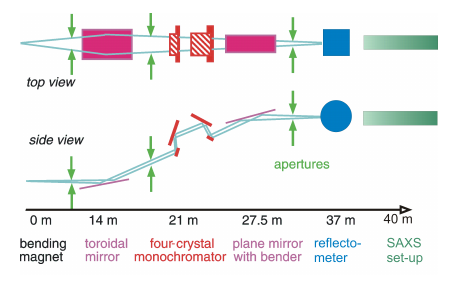
\includegraphics{Figures/FCMScheme.png}}
		\caption[Diagram of the Four-crystal monochromator beamline.]{A scheme of the FCM beamline in the PTB laboratory at BESSY II. The distance of each component to the bending magnet is shown.}
		\label{fig:FCMScheme}
\end{figure*}

At 14 m from the bending magnet, a Pt-coated toroidal mirror is located to focus the beam in the horizontal direction and to collimate it in the vertical direction. The radiation coming from the bending magnet is monochromatised further downstream by a set of 4 single crystals which reflect the light according to the Bragg's law for the (1 1 1) reflection. As the 4 crystals are mounted on two wheels (one on the rotation center and one parallelly aligned), the rotation angle of the wheel $\Theta$ defines the energy of the outgoing photon beam by $E=\frac{\sqrt{3}h c}{2a\sin{\Theta}}$, where $a$ is the lattice constant of the crystal.

Two types of exchangeable crystal sets, Si ($a=0.543$ nm) and InSb ($a=0.648$ nm), are available to cover the energy range from 1.75 keV to 10 keV. The convolution of the 4 Bragg reflections provides a very high energy resolving power ($E/\Delta E = 10^4 $) through the full energy range. Besides, the geometric disposition of the crystals fixes the position of the outgoing radiation. The monochromator is operated under a $10^{-8}$ mbar vacuum.

The energy is traced back to the well-known lattice constant of Si. The back-reflection of a silicon crystal at different lattice planes is measured at known energies and the energy is calibrated to the dips positions appearing when the Bragg condition is fulfilled. This approach was employed at the sensitive surface of the X-ray detector introduced in section \ref{sec:pilatus} for an energy range between 4 keV and 10 keV \citep{gollwitzer_diffraction_2014}. To check the accuracy of the energy calibration for daily measurements, a transmission scan around the K-edge of a copper foil (8980.5 eV) can be measured.

About 10 m before the sample chamber, a bendable plane mirror focuses the beam in the vertical direction. The mirror is coated with two different materials in separated areas. The Pt-coating is employed to maximize the reflectivity at energies above 4 keV, while the MgF$_2$ suppresses the higher orders at energies below 4 keV. The photon flux achieved with the different configurations available at the FCM beamline is shown in figure \ref{fig:FCMBeamlineFlux}, although it can vary depending on the precise disposition of the different apertures along the beam path.

\begin{figure}%[htbp]
	\centering
		% GNUPLOT: LaTeX picture with Postscript
\begingroup
  \makeatletter
  \providecommand\color[2][]{%
    \GenericError{(gnuplot) \space\space\space\@spaces}{%
      Package color not loaded in conjunction with
      terminal option `colourtext'%
    }{See the gnuplot documentation for explanation.%
    }{Either use 'blacktext' in gnuplot or load the package
      color.sty in LaTeX.}%
    \renewcommand\color[2][]{}%
  }%
  \providecommand\includegraphics[2][]{%
    \GenericError{(gnuplot) \space\space\space\@spaces}{%
      Package graphicx or graphics not loaded%
    }{See the gnuplot documentation for explanation.%
    }{The gnuplot epslatex terminal needs graphicx.sty or graphics.sty.}%
    \renewcommand\includegraphics[2][]{}%
  }%
  \providecommand\rotatebox[2]{#2}%
  \@ifundefined{ifGPcolor}{%
    \newif\ifGPcolor
    \GPcolortrue
  }{}%
  \@ifundefined{ifGPblacktext}{%
    \newif\ifGPblacktext
    \GPblacktextfalse
  }{}%
  % define a \g@addto@macro without @ in the name:
  \let\gplgaddtomacro\g@addto@macro
  % define empty templates for all commands taking text:
  \gdef\gplbacktext{}%
  \gdef\gplfronttext{}%
  \makeatother
  \ifGPblacktext
    % no textcolor at all
    \def\colorrgb#1{}%
    \def\colorgray#1{}%
  \else
    % gray or color?
    \ifGPcolor
      \def\colorrgb#1{\color[rgb]{#1}}%
      \def\colorgray#1{\color[gray]{#1}}%
      \expandafter\def\csname LTw\endcsname{\color{white}}%
      \expandafter\def\csname LTb\endcsname{\color{black}}%
      \expandafter\def\csname LTa\endcsname{\color{black}}%
      \expandafter\def\csname LT0\endcsname{\color[rgb]{1,0,0}}%
      \expandafter\def\csname LT1\endcsname{\color[rgb]{0,1,0}}%
      \expandafter\def\csname LT2\endcsname{\color[rgb]{0,0,1}}%
      \expandafter\def\csname LT3\endcsname{\color[rgb]{1,0,1}}%
      \expandafter\def\csname LT4\endcsname{\color[rgb]{0,1,1}}%
      \expandafter\def\csname LT5\endcsname{\color[rgb]{1,1,0}}%
      \expandafter\def\csname LT6\endcsname{\color[rgb]{0,0,0}}%
      \expandafter\def\csname LT7\endcsname{\color[rgb]{1,0.3,0}}%
      \expandafter\def\csname LT8\endcsname{\color[rgb]{0.5,0.5,0.5}}%
    \else
      % gray
      \def\colorrgb#1{\color{black}}%
      \def\colorgray#1{\color[gray]{#1}}%
      \expandafter\def\csname LTw\endcsname{\color{white}}%
      \expandafter\def\csname LTb\endcsname{\color{black}}%
      \expandafter\def\csname LTa\endcsname{\color{black}}%
      \expandafter\def\csname LT0\endcsname{\color{black}}%
      \expandafter\def\csname LT1\endcsname{\color{black}}%
      \expandafter\def\csname LT2\endcsname{\color{black}}%
      \expandafter\def\csname LT3\endcsname{\color{black}}%
      \expandafter\def\csname LT4\endcsname{\color{black}}%
      \expandafter\def\csname LT5\endcsname{\color{black}}%
      \expandafter\def\csname LT6\endcsname{\color{black}}%
      \expandafter\def\csname LT7\endcsname{\color{black}}%
      \expandafter\def\csname LT8\endcsname{\color{black}}%
    \fi
  \fi
  \setlength{\unitlength}{0.0500bp}%
  \begin{picture}(5668.00,4534.00)%
    \gplgaddtomacro\gplbacktext{%
      \csname LTb\endcsname%
      \put(748,704){\makebox(0,0)[r]{\strut{}$10^{10}$}}%
      \csname LTb\endcsname%
      \put(748,3073){\makebox(0,0)[r]{\strut{}$10^{11}$}}%
      \csname LTb\endcsname%
      \put(1039,484){\makebox(0,0){\strut{} 2}}%
      \csname LTb\endcsname%
      \put(1568,484){\makebox(0,0){\strut{} 3}}%
      \csname LTb\endcsname%
      \put(2097,484){\makebox(0,0){\strut{} 4}}%
      \csname LTb\endcsname%
      \put(2626,484){\makebox(0,0){\strut{} 5}}%
      \csname LTb\endcsname%
      \put(3155,484){\makebox(0,0){\strut{} 6}}%
      \csname LTb\endcsname%
      \put(3684,484){\makebox(0,0){\strut{} 7}}%
      \csname LTb\endcsname%
      \put(4213,484){\makebox(0,0){\strut{} 8}}%
      \csname LTb\endcsname%
      \put(4742,484){\makebox(0,0){\strut{} 9}}%
      \csname LTb\endcsname%
      \put(5271,484){\makebox(0,0){\strut{} 10}}%
      \put(176,2486){\rotatebox{-270}{\makebox(0,0){\strut{}Photon flux / s$^{-1}$}}}%
      \put(3075,154){\makebox(0,0){\strut{}Photon Energy / keV}}%
    }%
    \gplgaddtomacro\gplfronttext{%
      \csname LTb\endcsname%
      \put(4284,4096){\makebox(0,0)[r]{\strut{}InSb(111) / MgF$_2$}}%
      \csname LTb\endcsname%
      \put(4284,3876){\makebox(0,0)[r]{\strut{}Si(111) / Pt}}%
      \csname LTb\endcsname%
      \put(4284,3656){\makebox(0,0)[r]{\strut{}Si(111) / MgF$_2$}}%
    }%
    \gplbacktext
    \put(0,0){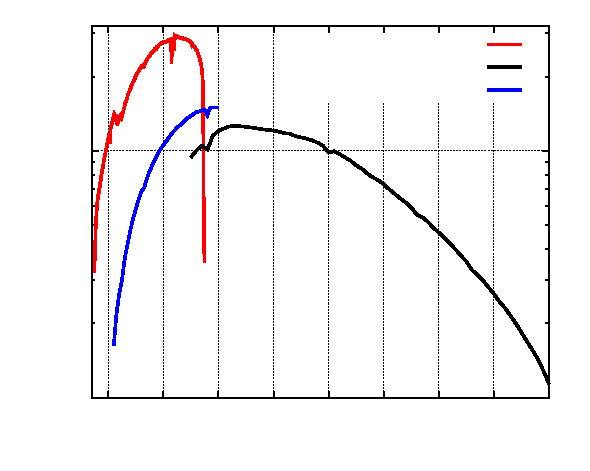
\includegraphics{FCMBeamlineFlux}}%
    \gplfronttext
  \end{picture}%
\endgroup

		\caption[Photon flux of the FCM beamline.]{Photon flux of the FCM beamline using different crystals (InSb(111) and Si(111)) and mirror coatings (MgF$_2$ and Pt) at standard operation (300 mA).}
		\label{fig:FCMBeamlineFlux}
\end{figure}

The first slit behind the bending magnet is used to limit the acceptance angle of the radiation into the monochromator. Two moveable slits more are employed downstream to block the parasitic scattering. A germanium 520 $\mu$m circular pinhole (Scatex, Incoatec, Geesthacht, Germany) situated before the sample chamber shapes the photon beam into a circular spot on the sample and strongly reduces the parasitic radiation. A 8 $\mu$m thick silicon photodiode diode is installed behind these components and can monitor continuously the incoming photon flux for energies above 3 keV.

\subsection{UHV X-ray reflectometer}

The sample chamber is situated 37 m away from the dipole i.e. bending magnet, right behind the flux monitor diode. The UHV X-ray reflectometer disposes of a large volume (60 cm diameter and 70 cm length) which is fully evacuated to reach pressures of approximately $10^{-7}$ mbar. High vacuum is needed to perform experiments at the low energies accessible at the FCM beamline, as the attenuation length of air at energies below 2 keV is less than 1 cm. A smaller lock chamber connected to the sample chamber by a 200 mm diameter flange is used to exchange samples without breaking the vacuum of the larger UHV X-ray reflectometer.

The motors of the sample holder can be moved linearly in three mutually perpendicular directions with very high precision and reproducibility. The broad range of the $x$-motor perpendicular to the incoming beam (160 mm) permits the measurement of different sample capillaries (ca. 20) at once without venting the chamber for exchanging the sample.

The large volume of the reflectometer provides enough space to allocate other components close to the sample holder. For example, about 10 cm before the sample position, a 1 mm circular guard pinhole (Incoatec, Geesthacht, Germany) is installed to remove the parasitic scattering resulting from the collimating system. Behind the sample, the transmitted radiation is measured with a (10 x 10) mm$^2$ silicon photodiode. The thick Can500C diode (Canberra, Meriden, USA) is capable of measuring through the entire beamline energy range, from 1.75 keV to 10 keV, and is calibrated against a cryogenic electric substitution radiometer with a relative uncertainty of 1 $\%$ \citep{krumrey_high-accuracy_2001}.

\section{SAXS Setup}
\label{sec:SAXS_experimental}

The intensity scattered by the sample is recorded at a certain distance behind the sample (sample-detector distance) with an area X-ray detector mounted on the HZB SAXS instrument and connected to the sample chamber. Typically, long sample-detector distances are required to access the small angles employed in SAXS experiments.

\subsection{X-ray area detector}
\label{sec:pilatus}

The scattered X-ray photons are collected by a large-area hybrid pixel detector. The Pilatus 1M (Dectris Ltd, Baden, Switzerland) has a sensitive surface of (179 x 169) mm$^2$ and consists of a silicon pixel matrix with a pixel size of $d = (172.1 \pm 0.2)$ $\mu$m which operates in single-photon counting mode, providing very low darkcount rates, very good signal-to-noise ratios and a high dynamic range. For instance, the detector quantum efficiency is about 97 $\%$ at 8 keV using the ultra-high gain mode and almost 86 $\%$ at 4 keV \citep{wernecke_characterization_2014}.

Besides, the Pilatus 1M detector was modified to operate under vacuum to cover the full energetic range available at the beamline, down to 1.75 keV. The windowless detector is directly connected to the sample chamber with an evacuated bellow and cooled down at 5 to 10 $^{\circ}$C. The narrow point-spread function of the detector and the available low energies increase the momentum transfer resolution and the accessible $q$-range.

A moveable beamstop mounted at thin wires is installed just in front of the detector to block the intense transmitted photon beam, avoiding saturation effects in the central pixels. The beamstop is constructed within a funnel-like cavity ($\oslash$ 5 mm) to reduce geometrically the reflections on the beamstop surface, which are damped by the cavity. Since April 2016, a silicon photodiode with a sensitive area of (2.5 x 2.5) mm$^2$ (S10356-01, Hamamatsu, Shizuoka, Japan) covers the beamstop to monitor the sample transmission during the experiment, revealing the possible radiation damage of the sample.

\subsection{HZB SAXS instrument and WAXS configuration}
\label{sec:WAXS_experimental}

The in-vacuum Pilatus 1M detector is mounted on the SAXS instrument of the Helmholtz-Zentrum Berlin (HZB), which is connected via a $\oslash$100 mm flange to the UHV X-ray Reflectometer. The HZB-SAXS apparatus is equipped with a large below system and a motorized stage that can vary the sample-detector distance continuously between 2.3 m and 4.6 m in vacuum (about $10^{-4}$ mbar) with an uncertainty of 20 $\mu$m. 

\begin{table}[]
\centering
\caption[Two different SAXS experimental setups and the accessible $q$-range.]{Two different experimental setups which span the accessible $q$-range for almost 3 decades. The overall maximum and minimum accessible $q$-values are highlighted in bold letters.}
\label{tab:qrange}
\begin{tabular}{|l|c|c|}
\hline
              & \textbf{SAXS} & \textbf{WAXS} \\ \hline
Distance (mm) & 4540          & 760           \\ \hline
Energy (eV)   & 4000          & 10000         \\ \hline
$q_{\text{min}}$ (nm$^{-1}$)   & \textbf{0.015}         & 0.2          \\ \hline
$q_{\text{max}}$ (nm$^{-1}$)   & 0.56             & \textbf{7}             \\ \hline
\end{tabular}
\end{table}

Complementary to the HZB-SAXS instrument, the sample-detector distance can be reduced down to about 760 mm by attaching the X-ray detector directly to the sample chamber, increasing the scattering angles to around $8^{\circ}$. This short-distance setup, or Wide-angle X-ray Scattering (WAXS) configuration, is used for the study of nanoparticles with diameters below 10 nm, whose characteristic features appear beyond 1 nm$^{-1}$. The accessible $q$-range of this setup is summarized in table \ref{tab:qrange} for the high-energy case, which provides the highest $q$-value available. Similarly, the table shows the limit $q$-values achieved with the HZB-SAXS apparatus at low-energy.

\subsubsection{Calibration of the sample-detector distance}

In small-angle scattering experiments, it is crucial to know precisely the distance between the irradiated sample and the detector, in order to calibrate the momentum transfer $q$. Typically, a calibration standard material with a well-known crystal lattice parameter is employed, which produces well-defined diffraction rings in the low-angle region. A material extensively used is dry rat-tail tendon collagen, with a $d$-spacing of 650 \AA \citep{amenitsch_performance_1997}, corresponding to $q=0.097$ nm$^{-1}$. The degradation of this material upon prolonged radiation suggested the use of harder calibrants such as silver behenate (CH$_3$(CH$_2$)$_{20}$COO$\cdot$Ag) \citep{huang_x-ray_1993}.

AgBehe has a very narrow diffraction ring at $q=1.0763$ nm$^{-1}$, arising from a long-period spacing ($d_{001}$) value of 5.836 nm \citep{blanton_jcpdsinternational_1995}, although this value depends slightly on the synthesis. A deviation of 0.5 $\%$ in the diffraction peak position could be observed for different sample preparations. In order to increase the accuracy of the calibration, the sample-detector distance was determined by the detection of the scattering pattern of AgBehe at different positions of the HZB SAXS instrument, measured with the built-in 3 m long Heidenhain optical encoder. By triangulating the radius of the diffraction ring to the source point, as depicted in figure \ref{fig:DistanceCalibrationSAXS}, the sample-detector distance is obtained in a traceable way.

\begin{figure*}
	\centering
\subfloat[Distance Calibration]{\resizebox{0.5\linewidth}{!}{\figfont{12pt}% GNUPLOT: LaTeX picture with Postscript
\begingroup
  \makeatletter
  \providecommand\color[2][]{%
    \GenericError{(gnuplot) \space\space\space\@spaces}{%
      Package color not loaded in conjunction with
      terminal option `colourtext'%
    }{See the gnuplot documentation for explanation.%
    }{Either use 'blacktext' in gnuplot or load the package
      color.sty in LaTeX.}%
    \renewcommand\color[2][]{}%
  }%
  \providecommand\includegraphics[2][]{%
    \GenericError{(gnuplot) \space\space\space\@spaces}{%
      Package graphicx or graphics not loaded%
    }{See the gnuplot documentation for explanation.%
    }{The gnuplot epslatex terminal needs graphicx.sty or graphics.sty.}%
    \renewcommand\includegraphics[2][]{}%
  }%
  \providecommand\rotatebox[2]{#2}%
  \@ifundefined{ifGPcolor}{%
    \newif\ifGPcolor
    \GPcolortrue
  }{}%
  \@ifundefined{ifGPblacktext}{%
    \newif\ifGPblacktext
    \GPblacktextfalse
  }{}%
  % define a \g@addto@macro without @ in the name:
  \let\gplgaddtomacro\g@addto@macro
  % define empty templates for all commands taking text:
  \gdef\gplbacktext{}%
  \gdef\gplfronttext{}%
  \makeatother
  \ifGPblacktext
    % no textcolor at all
    \def\colorrgb#1{}%
    \def\colorgray#1{}%
  \else
    % gray or color?
    \ifGPcolor
      \def\colorrgb#1{\color[rgb]{#1}}%
      \def\colorgray#1{\color[gray]{#1}}%
      \expandafter\def\csname LTw\endcsname{\color{white}}%
      \expandafter\def\csname LTb\endcsname{\color{black}}%
      \expandafter\def\csname LTa\endcsname{\color{black}}%
      \expandafter\def\csname LT0\endcsname{\color[rgb]{1,0,0}}%
      \expandafter\def\csname LT1\endcsname{\color[rgb]{0,1,0}}%
      \expandafter\def\csname LT2\endcsname{\color[rgb]{0,0,1}}%
      \expandafter\def\csname LT3\endcsname{\color[rgb]{1,0,1}}%
      \expandafter\def\csname LT4\endcsname{\color[rgb]{0,1,1}}%
      \expandafter\def\csname LT5\endcsname{\color[rgb]{1,1,0}}%
      \expandafter\def\csname LT6\endcsname{\color[rgb]{0,0,0}}%
      \expandafter\def\csname LT7\endcsname{\color[rgb]{1,0.3,0}}%
      \expandafter\def\csname LT8\endcsname{\color[rgb]{0.5,0.5,0.5}}%
    \else
      % gray
      \def\colorrgb#1{\color{black}}%
      \def\colorgray#1{\color[gray]{#1}}%
      \expandafter\def\csname LTw\endcsname{\color{white}}%
      \expandafter\def\csname LTb\endcsname{\color{black}}%
      \expandafter\def\csname LTa\endcsname{\color{black}}%
      \expandafter\def\csname LT0\endcsname{\color{black}}%
      \expandafter\def\csname LT1\endcsname{\color{black}}%
      \expandafter\def\csname LT2\endcsname{\color{black}}%
      \expandafter\def\csname LT3\endcsname{\color{black}}%
      \expandafter\def\csname LT4\endcsname{\color{black}}%
      \expandafter\def\csname LT5\endcsname{\color{black}}%
      \expandafter\def\csname LT6\endcsname{\color{black}}%
      \expandafter\def\csname LT7\endcsname{\color{black}}%
      \expandafter\def\csname LT8\endcsname{\color{black}}%
    \fi
  \fi
    \setlength{\unitlength}{0.0500bp}%
    \ifx\gptboxheight\undefined%
      \newlength{\gptboxheight}%
      \newlength{\gptboxwidth}%
      \newsavebox{\gptboxtext}%
    \fi%
    \setlength{\fboxrule}{0.5pt}%
    \setlength{\fboxsep}{1pt}%
\begin{picture}(5668.00,4534.00)%
    \gplgaddtomacro\gplbacktext{%
      \csname LTb\endcsname%
      \put(264,2622){\makebox(0,0)[r]{\strut{}$300$}}%
      \csname LTb\endcsname%
      \put(264,3067){\makebox(0,0)[r]{\strut{}$400$}}%
      \csname LTb\endcsname%
      \put(264,3511){\makebox(0,0)[r]{\strut{}$500$}}%
      \csname LTb\endcsname%
      \put(264,3955){\makebox(0,0)[r]{\strut{}$600$}}%
      \csname LTb\endcsname%
      \put(264,4399){\makebox(0,0)[r]{\strut{}$700$}}%
      \csname LTb\endcsname%
      \put(618,2047){\makebox(0,0){\strut{}}}%
      \csname LTb\endcsname%
      \put(1726,2047){\makebox(0,0){\strut{}}}%
      \csname LTb\endcsname%
      \put(2834,2047){\makebox(0,0){\strut{}}}%
      \csname LTb\endcsname%
      \put(3941,2047){\makebox(0,0){\strut{}}}%
      \csname LTb\endcsname%
      \put(5049,2047){\makebox(0,0){\strut{}}}%
    }%
    \gplgaddtomacro\gplfronttext{%
      \csname LTb\endcsname%
      \put(-242,3509){\rotatebox{-270}{\makebox(0,0){\strut{}Radius size / pixel}}}%
      \csname LTb\endcsname%
      \put(1314,4234){\makebox(0,0)[r]{\strut{}AgBehe}}%
      \csname LTb\endcsname%
      \put(1314,3904){\makebox(0,0)[r]{\strut{}SBA}}%
    }%
    \gplgaddtomacro\gplbacktext{%
      \csname LTb\endcsname%
      \put(264,721){\makebox(0,0)[r]{\strut{}$-3$}}%
      \csname LTb\endcsname%
      \put(264,1036){\makebox(0,0)[r]{\strut{}$-2$}}%
      \csname LTb\endcsname%
      \put(264,1352){\makebox(0,0)[r]{\strut{}$-1$}}%
      \csname LTb\endcsname%
      \put(264,1667){\makebox(0,0)[r]{\strut{}$0$}}%
      \csname LTb\endcsname%
      \put(264,1983){\makebox(0,0)[r]{\strut{}$1$}}%
      \csname LTb\endcsname%
      \put(618,343){\makebox(0,0){\strut{}2500}}%
      \csname LTb\endcsname%
      \put(1726,343){\makebox(0,0){\strut{}3000}}%
      \csname LTb\endcsname%
      \put(2834,343){\makebox(0,0){\strut{}3500}}%
      \csname LTb\endcsname%
      \put(3941,343){\makebox(0,0){\strut{}4000}}%
      \csname LTb\endcsname%
      \put(5049,343){\makebox(0,0){\strut{}4500}}%
    }%
    \gplgaddtomacro\gplfronttext{%
      \csname LTb\endcsname%
      \put(-209,1305){\rotatebox{-270}{\makebox(0,0){\strut{}Residuals / pixel}}}%
      \put(2833,46){\makebox(0,0){\strut{}Measured distance / mm}}%
    }%
    \gplbacktext
    \put(0,0){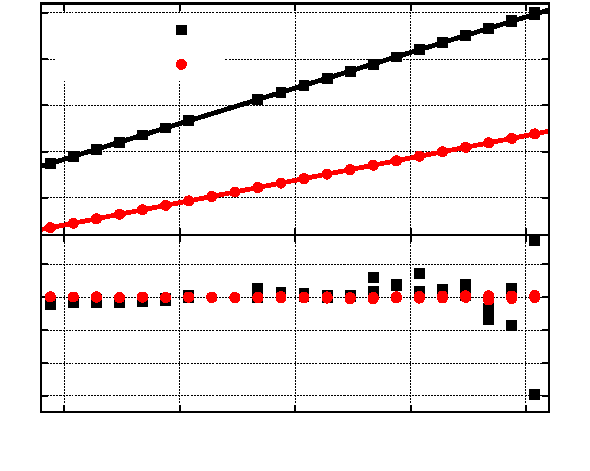
\includegraphics{DistanceCalibrationSAXS}}%
    \gplfronttext
  \end{picture}%
\endgroup
}\label{fig:DistanceCalibrationSAXS}}
		\subfloat[AgBehe at large distance]{\resizebox{0.35\linewidth}{!}{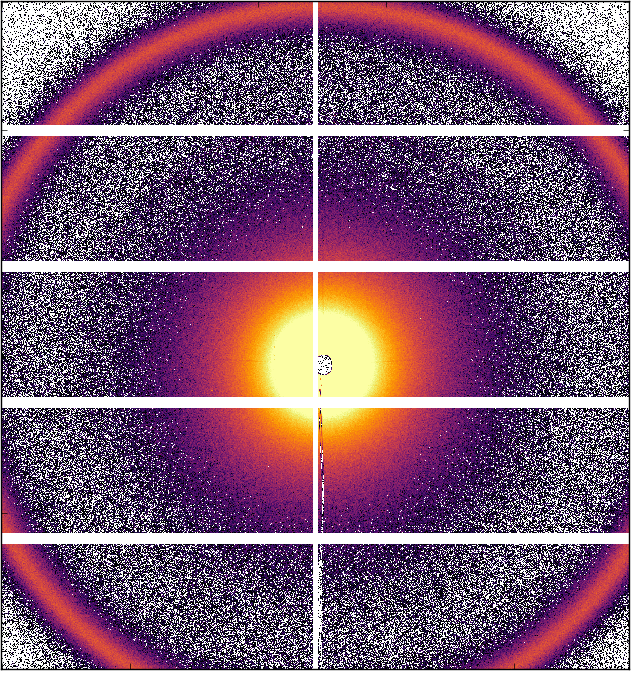
\includegraphics{Figures/AgBeheSAXSLongDistance_edit.png}}\label{fig:AgBeheSAXSLongDistance}}
		\caption[Sample-to-detector distance calibration and scattering pattern of AgBehe at large distance.]{Sample-to-detector distance calibration: a) Radius of the diffraction ring of AgBehe and SBA-15 as a function of the sample-detector distance. A linear function is fitted to obtain the source point distance. The residuals of the fitting are shown in the bottom plot. b) Scattering pattern of AgBehe measured at a distance of 3638.2 mm. At such long sample-to-detector distances, the diffraction rings exceeds the detector area and the associated uncertainty increases.}
\end{figure*}

By measuring the AgBehe pattern along a distance range of 2200 mm with 100 mm steps at 8000 eV, the relative uncertainty associated to the linear fitting is 0.03 $\%$, corresponding to 1.5 mm. As observed in the residuals of the fitting in figure \ref{fig:DistanceCalibrationSAXS}, the deviation increases for long distances, due to the relatively small $d$-spacing of AgBehe, disabling the use of distances larger than $\sim 3600$ mm. In figure \ref{fig:AgBeheSAXSLongDistance}, it is visible how the diffraction ring surpasses the surface of the detector at a distance of 3638.2 mm and, thus, diminishes the accuracy of the peak determination.

By using a material with lower $q$-value, such as the templated mesoporous silica SBA-15 ($q=0.681$ nm$^{-1}$ \citep{zhao_triblock_1998}), this limitation can be mitigated as shown in figure \ref{fig:DistanceCalibrationSAXS}, where the residuals of SBA are minimal for the entire distance range. By using SBA (kindly provided by R. Schmack (Technische Universität Berlin, Germany)) and increasing the accessible distance range, the relative uncertainty of the fit decreases in a factor 5, reaching an uncertainty of 0.004 $\%$ (0.2 mm) when measuring with 50 mm steps. This improvement is also related with the narrower diffraction peak of SBA-15 (FWHM/$q=2.6\;\%$) in comparison to AgBehe (5.5 $\%$).

Although the fit uncertainty is smaller in the SBA case, the position and shape of diffraction peak depend strongly on the sample preparation (e.g. template pore size). For the same polymer template, the $q$-value of the ring can vary until 1 $\%$ for different thermal treatments and radiation damage effects are visible for short calcination times. On the other side, prolonged beam exposure of AgBehe can damage the sample as well and create small silver nanoparticles, which increase the scattering background \citep{liu_thermal_2006}. The choice of the calibration standard depends strictly on the needs of the experiment. Besides, the largest contributions to the sample-detector distance uncertainty come from the thickness of the sample (ca. 0.5 mm) and from the difference between the calibration with AgBehe and SBA-15 (also 0.5 mm). Normally the relative uncertainty associated with the distance calibration is $10^{-4}$, similar to the energy resolving power described in section \ref{sec:fcm}.

\section{Sample environment}
\label{sec:sample_environment}

The sample consists normally of a few microliters of nanoparticles in solution which are measured in a vacuum-proof container positioned inside the reflectometer. The sample environment must fulfill some requirements:

\begin{itemize}
        \item The container's material should minimize the unnecessary absorption of the X-ray photon flux by the sample environment.
        \item The container volume should be small enough to enable the measurement of valuable, limited samples.
        \item The optimal sample thickness for a transmission diffraction experiment is the inverse of its attenuation coefficient $\mu(E)$, which reduces the incoming intensity to $\sim37\;\%$. For example, the optimal thickness of water at 8000 eV is around 1 mm.
\end{itemize}

Typically, the samples are introduced in thin glass capillaries which maintain the temperature and pressure of the sample close to the ambient conditions. However, there are different sample environments which can be used depending on the requirements of the experiment. In this work, only nanoparticles suspended in aqueous media have been employed, allowing the use of a similar attenuation coefficient for almost all experiments.

\subsection{Round capillaries}

\begin{figure*}%[htbp]
	\centering
		\subfloat[Glass thickness]{\resizebox{0.48\linewidth}{!}{\figfont{13pt}% GNUPLOT: LaTeX picture with Postscript
\begingroup
  \makeatletter
  \providecommand\color[2][]{%
    \GenericError{(gnuplot) \space\space\space\@spaces}{%
      Package color not loaded in conjunction with
      terminal option `colourtext'%
    }{See the gnuplot documentation for explanation.%
    }{Either use 'blacktext' in gnuplot or load the package
      color.sty in LaTeX.}%
    \renewcommand\color[2][]{}%
  }%
  \providecommand\includegraphics[2][]{%
    \GenericError{(gnuplot) \space\space\space\@spaces}{%
      Package graphicx or graphics not loaded%
    }{See the gnuplot documentation for explanation.%
    }{The gnuplot epslatex terminal needs graphicx.sty or graphics.sty.}%
    \renewcommand\includegraphics[2][]{}%
  }%
  \providecommand\rotatebox[2]{#2}%
  \@ifundefined{ifGPcolor}{%
    \newif\ifGPcolor
    \GPcolortrue
  }{}%
  \@ifundefined{ifGPblacktext}{%
    \newif\ifGPblacktext
    \GPblacktextfalse
  }{}%
  % define a \g@addto@macro without @ in the name:
  \let\gplgaddtomacro\g@addto@macro
  % define empty templates for all commands taking text:
  \gdef\gplbacktext{}%
  \gdef\gplfronttext{}%
  \makeatother
  \ifGPblacktext
    % no textcolor at all
    \def\colorrgb#1{}%
    \def\colorgray#1{}%
  \else
    % gray or color?
    \ifGPcolor
      \def\colorrgb#1{\color[rgb]{#1}}%
      \def\colorgray#1{\color[gray]{#1}}%
      \expandafter\def\csname LTw\endcsname{\color{white}}%
      \expandafter\def\csname LTb\endcsname{\color{black}}%
      \expandafter\def\csname LTa\endcsname{\color{black}}%
      \expandafter\def\csname LT0\endcsname{\color[rgb]{1,0,0}}%
      \expandafter\def\csname LT1\endcsname{\color[rgb]{0,1,0}}%
      \expandafter\def\csname LT2\endcsname{\color[rgb]{0,0,1}}%
      \expandafter\def\csname LT3\endcsname{\color[rgb]{1,0,1}}%
      \expandafter\def\csname LT4\endcsname{\color[rgb]{0,1,1}}%
      \expandafter\def\csname LT5\endcsname{\color[rgb]{1,1,0}}%
      \expandafter\def\csname LT6\endcsname{\color[rgb]{0,0,0}}%
      \expandafter\def\csname LT7\endcsname{\color[rgb]{1,0.3,0}}%
      \expandafter\def\csname LT8\endcsname{\color[rgb]{0.5,0.5,0.5}}%
    \else
      % gray
      \def\colorrgb#1{\color{black}}%
      \def\colorgray#1{\color[gray]{#1}}%
      \expandafter\def\csname LTw\endcsname{\color{white}}%
      \expandafter\def\csname LTb\endcsname{\color{black}}%
      \expandafter\def\csname LTa\endcsname{\color{black}}%
      \expandafter\def\csname LT0\endcsname{\color{black}}%
      \expandafter\def\csname LT1\endcsname{\color{black}}%
      \expandafter\def\csname LT2\endcsname{\color{black}}%
      \expandafter\def\csname LT3\endcsname{\color{black}}%
      \expandafter\def\csname LT4\endcsname{\color{black}}%
      \expandafter\def\csname LT5\endcsname{\color{black}}%
      \expandafter\def\csname LT6\endcsname{\color{black}}%
      \expandafter\def\csname LT7\endcsname{\color{black}}%
      \expandafter\def\csname LT8\endcsname{\color{black}}%
    \fi
  \fi
  \setlength{\unitlength}{0.0500bp}%
  \begin{picture}(5668.00,4534.00)%
    \gplgaddtomacro\gplbacktext{%
    }%
    \gplgaddtomacro\gplfronttext{%
      \csname LTb\endcsname%
      \put(1241,736){\makebox(0,0){\strut{}-2}}%
      \put(1625,736){\makebox(0,0){\strut{}-1.5}}%
      \put(2009,736){\makebox(0,0){\strut{}-1}}%
      \put(2393,736){\makebox(0,0){\strut{}-0.5}}%
      \put(2777,736){\makebox(0,0){\strut{} 0}}%
      \put(3160,736){\makebox(0,0){\strut{} 0.5}}%
      \put(3544,736){\makebox(0,0){\strut{} 1}}%
      \put(3928,736){\makebox(0,0){\strut{} 1.5}}%
      \put(4312,736){\makebox(0,0){\strut{} 2}}%
      \put(4696,736){\makebox(0,0){\strut{} 2.5}}%
      \put(2834,406){\makebox(0,0){\strut{}Horizontal Position / mm}}%
      \put(801,1022){\makebox(0,0)[r]{\strut{} 5}}%
      \put(801,1304){\makebox(0,0)[r]{\strut{} 5.5}}%
      \put(801,1587){\makebox(0,0)[r]{\strut{} 6}}%
      \put(801,1869){\makebox(0,0)[r]{\strut{} 6.5}}%
      \put(801,2152){\makebox(0,0)[r]{\strut{} 7}}%
      \put(801,2433){\makebox(0,0)[r]{\strut{} 7.5}}%
      \put(801,2715){\makebox(0,0)[r]{\strut{} 8}}%
      \put(801,2998){\makebox(0,0)[r]{\strut{} 8.5}}%
      \put(801,3280){\makebox(0,0)[r]{\strut{} 9}}%
      \put(801,3563){\makebox(0,0)[r]{\strut{} 9.5}}%
      \put(207,2377){\rotatebox{-270}{\makebox(0,0){\strut{}Vertical Position / mm}}}%
      \put(5107,1022){\makebox(0,0)[l]{\strut{}-2}}%
      \put(5107,1473){\makebox(0,0)[l]{\strut{}-1.5}}%
      \put(5107,1925){\makebox(0,0)[l]{\strut{}-1}}%
      \put(5107,2377){\makebox(0,0)[l]{\strut{}-0.5}}%
      \put(5107,2828){\makebox(0,0)[l]{\strut{} 0}}%
      \put(5107,3280){\makebox(0,0)[l]{\strut{} 0.5}}%
      \put(5107,3732){\makebox(0,0)[l]{\strut{} 1}}%
      \put(5701,2377){\rotatebox{270}{\makebox(0,0){\strut{}Deviation /$\%$}}}%
    }%
    \gplbacktext
    \put(0,0){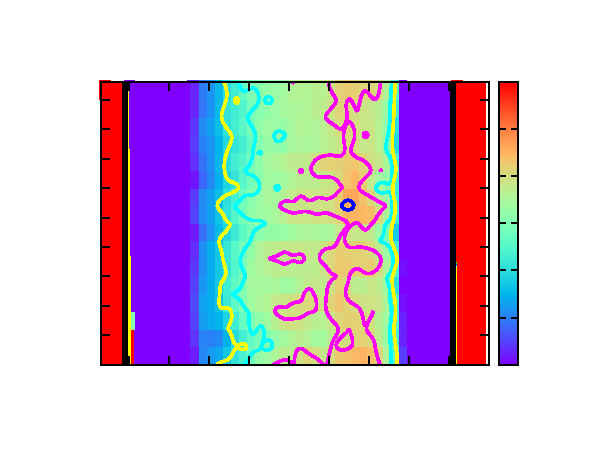
\includegraphics{HilgenbergHomogeneity}}%
    \gplfronttext
  \end{picture}%
\endgroup
}\label{fig:HilgenbergHomogeneity}}
		\subfloat[Sample thickness]{\resizebox{0.48\linewidth}{!}{\figfont{13pt}% GNUPLOT: LaTeX picture with Postscript
\begingroup
  \makeatletter
  \providecommand\color[2][]{%
    \GenericError{(gnuplot) \space\space\space\@spaces}{%
      Package color not loaded in conjunction with
      terminal option `colourtext'%
    }{See the gnuplot documentation for explanation.%
    }{Either use 'blacktext' in gnuplot or load the package
      color.sty in LaTeX.}%
    \renewcommand\color[2][]{}%
  }%
  \providecommand\includegraphics[2][]{%
    \GenericError{(gnuplot) \space\space\space\@spaces}{%
      Package graphicx or graphics not loaded%
    }{See the gnuplot documentation for explanation.%
    }{The gnuplot epslatex terminal needs graphicx.sty or graphics.sty.}%
    \renewcommand\includegraphics[2][]{}%
  }%
  \providecommand\rotatebox[2]{#2}%
  \@ifundefined{ifGPcolor}{%
    \newif\ifGPcolor
    \GPcolortrue
  }{}%
  \@ifundefined{ifGPblacktext}{%
    \newif\ifGPblacktext
    \GPblacktextfalse
  }{}%
  % define a \g@addto@macro without @ in the name:
  \let\gplgaddtomacro\g@addto@macro
  % define empty templates for all commands taking text:
  \gdef\gplbacktext{}%
  \gdef\gplfronttext{}%
  \makeatother
  \ifGPblacktext
    % no textcolor at all
    \def\colorrgb#1{}%
    \def\colorgray#1{}%
  \else
    % gray or color?
    \ifGPcolor
      \def\colorrgb#1{\color[rgb]{#1}}%
      \def\colorgray#1{\color[gray]{#1}}%
      \expandafter\def\csname LTw\endcsname{\color{white}}%
      \expandafter\def\csname LTb\endcsname{\color{black}}%
      \expandafter\def\csname LTa\endcsname{\color{black}}%
      \expandafter\def\csname LT0\endcsname{\color[rgb]{1,0,0}}%
      \expandafter\def\csname LT1\endcsname{\color[rgb]{0,1,0}}%
      \expandafter\def\csname LT2\endcsname{\color[rgb]{0,0,1}}%
      \expandafter\def\csname LT3\endcsname{\color[rgb]{1,0,1}}%
      \expandafter\def\csname LT4\endcsname{\color[rgb]{0,1,1}}%
      \expandafter\def\csname LT5\endcsname{\color[rgb]{1,1,0}}%
      \expandafter\def\csname LT6\endcsname{\color[rgb]{0,0,0}}%
      \expandafter\def\csname LT7\endcsname{\color[rgb]{1,0.3,0}}%
      \expandafter\def\csname LT8\endcsname{\color[rgb]{0.5,0.5,0.5}}%
    \else
      % gray
      \def\colorrgb#1{\color{black}}%
      \def\colorgray#1{\color[gray]{#1}}%
      \expandafter\def\csname LTw\endcsname{\color{white}}%
      \expandafter\def\csname LTb\endcsname{\color{black}}%
      \expandafter\def\csname LTa\endcsname{\color{black}}%
      \expandafter\def\csname LT0\endcsname{\color{black}}%
      \expandafter\def\csname LT1\endcsname{\color{black}}%
      \expandafter\def\csname LT2\endcsname{\color{black}}%
      \expandafter\def\csname LT3\endcsname{\color{black}}%
      \expandafter\def\csname LT4\endcsname{\color{black}}%
      \expandafter\def\csname LT5\endcsname{\color{black}}%
      \expandafter\def\csname LT6\endcsname{\color{black}}%
      \expandafter\def\csname LT7\endcsname{\color{black}}%
      \expandafter\def\csname LT8\endcsname{\color{black}}%
    \fi
  \fi
  \setlength{\unitlength}{0.0500bp}%
  \begin{picture}(5668.00,4534.00)%
    \gplgaddtomacro\gplbacktext{%
    }%
    \gplgaddtomacro\gplfronttext{%
      \csname LTb\endcsname%
      \put(1241,736){\makebox(0,0){\strut{}-2}}%
      \put(2009,736){\makebox(0,0){\strut{}-1}}%
      \put(2777,736){\makebox(0,0){\strut{} 0}}%
      \put(3544,736){\makebox(0,0){\strut{} 1}}%
      \put(4312,736){\makebox(0,0){\strut{} 2}}%
      \put(2834,406){\makebox(0,0){\strut{}Horizontal Position / mm}}%
      \put(801,1323){\makebox(0,0)[r]{\strut{}-4}}%
      \put(801,1926){\makebox(0,0)[r]{\strut{}-2}}%
      \put(801,2527){\makebox(0,0)[r]{\strut{} 0}}%
      \put(801,3130){\makebox(0,0)[r]{\strut{} 2}}%
      \put(801,3732){\makebox(0,0)[r]{\strut{} 4}}%
      \put(471,2377){\rotatebox{-270}{\makebox(0,0){\strut{}Vertical Position / mm}}}%
      \put(5107,1473){\makebox(0,0)[l]{\strut{} 0.99}}%
      \put(5107,2377){\makebox(0,0)[l]{\strut{} 1}}%
      \put(5107,3280){\makebox(0,0)[l]{\strut{} 1.01}}%
      \put(5833,2377){\rotatebox{270}{\makebox(0,0){\strut{}Sample Thickness / mm}}}%
    }%
    \gplbacktext
    \put(0,0){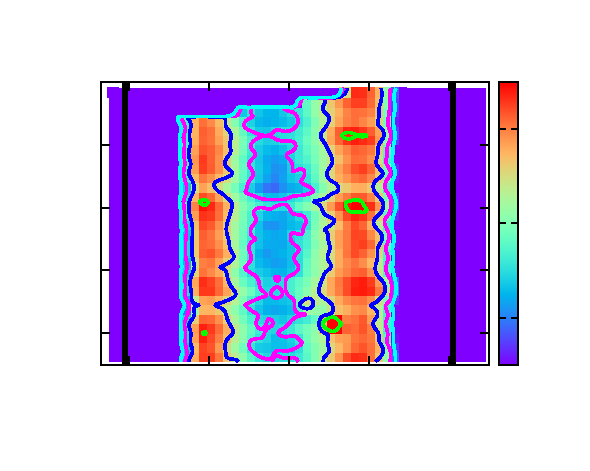
\includegraphics{WaterHomogeneity}}%
    \gplfronttext
  \end{picture}%
\endgroup
}\label{fig:WaterHomogeneity}}
		\caption[Homogeneity of the rectangular capillaries.]{Homogeneity of the rectangular capillaries: a) Deviation of the empty capillary tranmission, i.e. glass wall thickness, b) Sample thickness calculated from the water transmission of a filled capillary. }
\end{figure*}

For single-contrast SAXS measurements, borosilicate glass round capillaries of 100 mm length were used. They were purchased at WJM Glass (Berlin, Germany) and had a nominal inner diameter of 1 mm and a wall thickness of 10 $\mu$m. The sample is filled into the capillary with a long syringe (Sterican$\textregistered$21 x 4 3/4" , Braun, Melsungen, Germany), avoiding the contact of the needle with the capillary walls. The top end of the capillary is closed by welding.

The very narrow glass walls (with a density of about 2.23 g cm$^{-3}$) absorb only 14 $\%$ of the incoming flux at 8000 eV and produce very low scattering background. Therefore, these capillaries are suitable for standard SAXS measurements. Unfortunately, the capillaries sample thickness shows a significant deviation along the vertical axis and are inappropriate for measurements at different capillary heights, as needed for the continuous contrast variation technique.

\subsection{Rectangular capillaries}

The capillaries used for the contrast variation experiments are vacuum-proof borosilicate glass capillaries from Hilgenberg (Malsfeld, Germany) with a nominal rectangular cross section with outer dimensions of (4.2 $\pm$ 0.2) x (1.25 $\pm$ 0.05) mm$^2$ , a length of (80 $\pm$ 0.5) mm and a wall thickness of ca. 120 $\mu$m. The thicker glass walls reduce the transmitted intensity about 80 $\%$ at 8000 eV, but in contrast both the glass and sample thicknesses are very homogeneous for the entire capillary.

The transmission of an empty capillary is mapped in figure \ref{fig:HilgenbergHomogeneity}, where it can be observed that the deviation of the glass wall thickness is less than 2 $\%$ for an horizontal range of 2.5 mm (of a total width of 4.2 mm). This range is at least 5 times larger than the typical beam diameter, avoiding the convolution of different thicknesses in the measurement. Similarly, figure \ref{fig:WaterHomogeneity} depicts the sample thickness in the capillary, calculated from a capillary filled with water using the Beer-Lambert law, the glass transmission and the mass attenuation coefficient of water at 8000 eV, 10.37 cm$^{2}$ g$^{-1}$ \citep{hubbell_tables_1996}. The thickness of the sample introduced in the capillary is homogeneous within 2 $\%$ for a width range of ca. 2.5 mm. 

\begin{figure}%[htbp]
	\centering
	
%	        \resizebox{.85\linewidth}{!}{% GNUPLOT: LaTeX picture with Postscript
\begingroup
  \makeatletter
  \providecommand\color[2][]{%
    \GenericError{(gnuplot) \space\space\space\@spaces}{%
      Package color not loaded in conjunction with
      terminal option `colourtext'%
    }{See the gnuplot documentation for explanation.%
    }{Either use 'blacktext' in gnuplot or load the package
      color.sty in LaTeX.}%
    \renewcommand\color[2][]{}%
  }%
  \providecommand\includegraphics[2][]{%
    \GenericError{(gnuplot) \space\space\space\@spaces}{%
      Package graphicx or graphics not loaded%
    }{See the gnuplot documentation for explanation.%
    }{The gnuplot epslatex terminal needs graphicx.sty or graphics.sty.}%
    \renewcommand\includegraphics[2][]{}%
  }%
  \providecommand\rotatebox[2]{#2}%
  \@ifundefined{ifGPcolor}{%
    \newif\ifGPcolor
    \GPcolortrue
  }{}%
  \@ifundefined{ifGPblacktext}{%
    \newif\ifGPblacktext
    \GPblacktextfalse
  }{}%
  % define a \g@addto@macro without @ in the name:
  \let\gplgaddtomacro\g@addto@macro
  % define empty templates for all commands taking text:
  \gdef\gplbacktext{}%
  \gdef\gplfronttext{}%
  \makeatother
  \ifGPblacktext
    % no textcolor at all
    \def\colorrgb#1{}%
    \def\colorgray#1{}%
  \else
    % gray or color?
    \ifGPcolor
      \def\colorrgb#1{\color[rgb]{#1}}%
      \def\colorgray#1{\color[gray]{#1}}%
      \expandafter\def\csname LTw\endcsname{\color{white}}%
      \expandafter\def\csname LTb\endcsname{\color{black}}%
      \expandafter\def\csname LTa\endcsname{\color{black}}%
      \expandafter\def\csname LT0\endcsname{\color[rgb]{1,0,0}}%
      \expandafter\def\csname LT1\endcsname{\color[rgb]{0,1,0}}%
      \expandafter\def\csname LT2\endcsname{\color[rgb]{0,0,1}}%
      \expandafter\def\csname LT3\endcsname{\color[rgb]{1,0,1}}%
      \expandafter\def\csname LT4\endcsname{\color[rgb]{0,1,1}}%
      \expandafter\def\csname LT5\endcsname{\color[rgb]{1,1,0}}%
      \expandafter\def\csname LT6\endcsname{\color[rgb]{0,0,0}}%
      \expandafter\def\csname LT7\endcsname{\color[rgb]{1,0.3,0}}%
      \expandafter\def\csname LT8\endcsname{\color[rgb]{0.5,0.5,0.5}}%
    \else
      % gray
      \def\colorrgb#1{\color{black}}%
      \def\colorgray#1{\color[gray]{#1}}%
      \expandafter\def\csname LTw\endcsname{\color{white}}%
      \expandafter\def\csname LTb\endcsname{\color{black}}%
      \expandafter\def\csname LTa\endcsname{\color{black}}%
      \expandafter\def\csname LT0\endcsname{\color{black}}%
      \expandafter\def\csname LT1\endcsname{\color{black}}%
      \expandafter\def\csname LT2\endcsname{\color{black}}%
      \expandafter\def\csname LT3\endcsname{\color{black}}%
      \expandafter\def\csname LT4\endcsname{\color{black}}%
      \expandafter\def\csname LT5\endcsname{\color{black}}%
      \expandafter\def\csname LT6\endcsname{\color{black}}%
      \expandafter\def\csname LT7\endcsname{\color{black}}%
      \expandafter\def\csname LT8\endcsname{\color{black}}%
    \fi
  \fi
  \setlength{\unitlength}{0.0500bp}%
  \begin{picture}(5668.00,4534.00)%
    \gplgaddtomacro\gplbacktext{%
      \csname LTb\endcsname%
      \put(858,921){\makebox(0,0)[r]{\strut{} 0.07}}%
      \put(858,1964){\makebox(0,0)[r]{\strut{} 0.1}}%
      \put(858,3149){\makebox(0,0)[r]{\strut{} 0.15}}%
      \put(858,3990){\makebox(0,0)[r]{\strut{} 0.2}}%
      \put(1275,484){\makebox(0,0){\strut{}-4}}%
      \put(1846,484){\makebox(0,0){\strut{}-2}}%
      \put(2417,484){\makebox(0,0){\strut{} 0}}%
      \put(2988,484){\makebox(0,0){\strut{} 2}}%
      \put(3559,484){\makebox(0,0){\strut{} 4}}%
      \put(4129,484){\makebox(0,0){\strut{} 6}}%
      \put(4700,484){\makebox(0,0){\strut{} 8}}%
      \put(5271,484){\makebox(0,0){\strut{} 10}}%
      \put(220,2486){\rotatebox{-270}{\makebox(0,0){\strut{}Transmission}}}%
      \put(3130,154){\makebox(0,0){\strut{}Vertical position / mm}}%
    }%
    \gplgaddtomacro\gplfronttext{%
      \csname LTb\endcsname%
      \put(2475,3730){\makebox(0,0)[r]{\strut{}Transmission}}%
      \csname LTb\endcsname%
      \put(2475,3510){\makebox(0,0)[r]{\strut{}Glass only}}%
      \csname LTb\endcsname%
      \put(2475,3290){\makebox(0,0)[r]{\strut{}H$_2$O}}%
    }%
    \gplbacktext
    \put(0,0){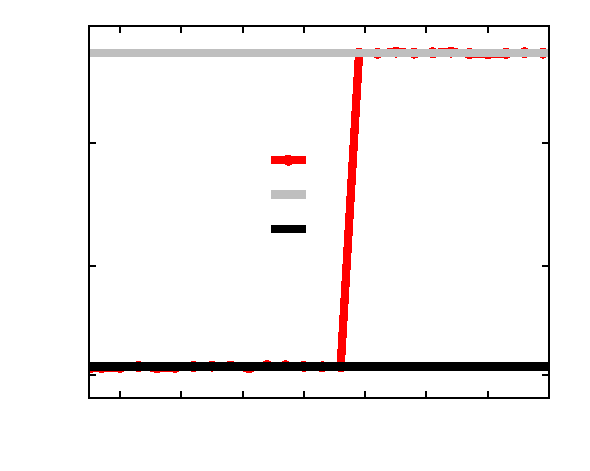
\includegraphics{GaldenCalibration}}%
    \gplfronttext
  \end{picture}%
\endgroup
}
	
		% GNUPLOT: LaTeX picture with Postscript
\begingroup
  \makeatletter
  \providecommand\color[2][]{%
    \GenericError{(gnuplot) \space\space\space\@spaces}{%
      Package color not loaded in conjunction with
      terminal option `colourtext'%
    }{See the gnuplot documentation for explanation.%
    }{Either use 'blacktext' in gnuplot or load the package
      color.sty in LaTeX.}%
    \renewcommand\color[2][]{}%
  }%
  \providecommand\includegraphics[2][]{%
    \GenericError{(gnuplot) \space\space\space\@spaces}{%
      Package graphicx or graphics not loaded%
    }{See the gnuplot documentation for explanation.%
    }{The gnuplot epslatex terminal needs graphicx.sty or graphics.sty.}%
    \renewcommand\includegraphics[2][]{}%
  }%
  \providecommand\rotatebox[2]{#2}%
  \@ifundefined{ifGPcolor}{%
    \newif\ifGPcolor
    \GPcolortrue
  }{}%
  \@ifundefined{ifGPblacktext}{%
    \newif\ifGPblacktext
    \GPblacktextfalse
  }{}%
  % define a \g@addto@macro without @ in the name:
  \let\gplgaddtomacro\g@addto@macro
  % define empty templates for all commands taking text:
  \gdef\gplbacktext{}%
  \gdef\gplfronttext{}%
  \makeatother
  \ifGPblacktext
    % no textcolor at all
    \def\colorrgb#1{}%
    \def\colorgray#1{}%
  \else
    % gray or color?
    \ifGPcolor
      \def\colorrgb#1{\color[rgb]{#1}}%
      \def\colorgray#1{\color[gray]{#1}}%
      \expandafter\def\csname LTw\endcsname{\color{white}}%
      \expandafter\def\csname LTb\endcsname{\color{black}}%
      \expandafter\def\csname LTa\endcsname{\color{black}}%
      \expandafter\def\csname LT0\endcsname{\color[rgb]{1,0,0}}%
      \expandafter\def\csname LT1\endcsname{\color[rgb]{0,1,0}}%
      \expandafter\def\csname LT2\endcsname{\color[rgb]{0,0,1}}%
      \expandafter\def\csname LT3\endcsname{\color[rgb]{1,0,1}}%
      \expandafter\def\csname LT4\endcsname{\color[rgb]{0,1,1}}%
      \expandafter\def\csname LT5\endcsname{\color[rgb]{1,1,0}}%
      \expandafter\def\csname LT6\endcsname{\color[rgb]{0,0,0}}%
      \expandafter\def\csname LT7\endcsname{\color[rgb]{1,0.3,0}}%
      \expandafter\def\csname LT8\endcsname{\color[rgb]{0.5,0.5,0.5}}%
    \else
      % gray
      \def\colorrgb#1{\color{black}}%
      \def\colorgray#1{\color[gray]{#1}}%
      \expandafter\def\csname LTw\endcsname{\color{white}}%
      \expandafter\def\csname LTb\endcsname{\color{black}}%
      \expandafter\def\csname LTa\endcsname{\color{black}}%
      \expandafter\def\csname LT0\endcsname{\color{black}}%
      \expandafter\def\csname LT1\endcsname{\color{black}}%
      \expandafter\def\csname LT2\endcsname{\color{black}}%
      \expandafter\def\csname LT3\endcsname{\color{black}}%
      \expandafter\def\csname LT4\endcsname{\color{black}}%
      \expandafter\def\csname LT5\endcsname{\color{black}}%
      \expandafter\def\csname LT6\endcsname{\color{black}}%
      \expandafter\def\csname LT7\endcsname{\color{black}}%
      \expandafter\def\csname LT8\endcsname{\color{black}}%
    \fi
  \fi
  \setlength{\unitlength}{0.0500bp}%
  \begin{picture}(5668.00,4534.00)%
    \gplgaddtomacro\gplbacktext{%
      \csname LTb\endcsname%
      \put(858,921){\makebox(0,0)[r]{\strut{} 0.07}}%
      \put(858,1964){\makebox(0,0)[r]{\strut{} 0.1}}%
      \put(858,3149){\makebox(0,0)[r]{\strut{} 0.15}}%
      \put(858,3990){\makebox(0,0)[r]{\strut{} 0.2}}%
      \put(1275,484){\makebox(0,0){\strut{}-4}}%
      \put(1846,484){\makebox(0,0){\strut{}-2}}%
      \put(2417,484){\makebox(0,0){\strut{} 0}}%
      \put(2988,484){\makebox(0,0){\strut{} 2}}%
      \put(3559,484){\makebox(0,0){\strut{} 4}}%
      \put(4129,484){\makebox(0,0){\strut{} 6}}%
      \put(4700,484){\makebox(0,0){\strut{} 8}}%
      \put(5271,484){\makebox(0,0){\strut{} 10}}%
      \put(220,2486){\rotatebox{-270}{\makebox(0,0){\strut{}Transmission}}}%
      \put(3130,154){\makebox(0,0){\strut{}Vertical position / mm}}%
    }%
    \gplgaddtomacro\gplfronttext{%
      \csname LTb\endcsname%
      \put(2475,3730){\makebox(0,0)[r]{\strut{}Transmission}}%
      \csname LTb\endcsname%
      \put(2475,3510){\makebox(0,0)[r]{\strut{}Glass only}}%
      \csname LTb\endcsname%
      \put(2475,3290){\makebox(0,0)[r]{\strut{}H$_2$O}}%
    }%
    \gplbacktext
    \put(0,0){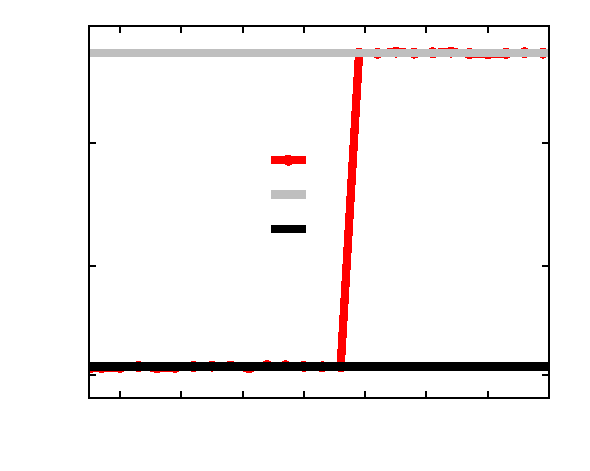
\includegraphics{GaldenCalibration}}%
    \gplfronttext
  \end{picture}%
\endgroup

		\caption[X-ray transmission of a rectangular capillary half-filled with water]{X-ray transmission of a rectangular capillary half-filled with water along the main vertical axis situated at $x=-0.15$ mm.}
		\label{fig:GaldenCalibration}
\end{figure}

From these figures, it is clear that the homogeneity of the sample environment is even better along the main vertical axis of the capillary. Figure \ref{fig:GaldenCalibration} shows the measured X-ray transmission of a half-filled capillary along its vertical axis (at the horizontal position -0.15 mm). For example, the glass transmission within a 6 mm vertical range is 20.1 $\%$, with an associated relative uncertainty of $\delta_r T =0.6 \; \%$. By calculating $\delta_r d = \frac{\delta_r T}{log(T)}$ where $T$ is the glass transmission, the relative uncertainty of the glass thickness is $\delta_r d = 0.4 \; \%$. Analogously, the uncertainty of the water transmission is 0.9 $\%$ and the sample thickness has an uncertainty of 0.9 $\%$ along the vertical axis.

These rectangular capillaries are a very suitable sample environment for measurements which require a high homogeneity along the vertical axis of the capillary. The thickness of the wall varies only by 0.4 $\%$ and the sample thickness less than 0.9 $\%$, although the thick glass walls reduce considerably the transmitted intensity and produce larger background scattering than the round capillaries.

\subsection{Cell for low-energies}

Samples with larger structures require the measurement of scattering curves at lower $q$-values. To extend the measurable $q$-range, one possibility is to reduce the photon energy, though this involves reducing the sample thickness, due to the short penetration length of X-rays at low energies. Therefore, a custom-made sample holder is used utilizing silicon-nitride windows (NX7150E, Norcada Inc., Edmonton, Canada). The 500 nm thickness windows produce very low scattering and have a negligible absorbance ($<5\;\%$) for energies above 4000 eV.

A polymeric 100 $\mu$m ring cut with a microtome is used as spacer between the 2 windows, in order to achieve the desired 120 $\mu$m sample thickness which optimizes the intensity attenuation at 4000 eV. The access to smaller $q$-values using this cell is shown in \cite{varga_towards_2014}, where a value of $q=0.015$ nm$^{-1}$ is achieved.

\begin{figure}%[htbp]
		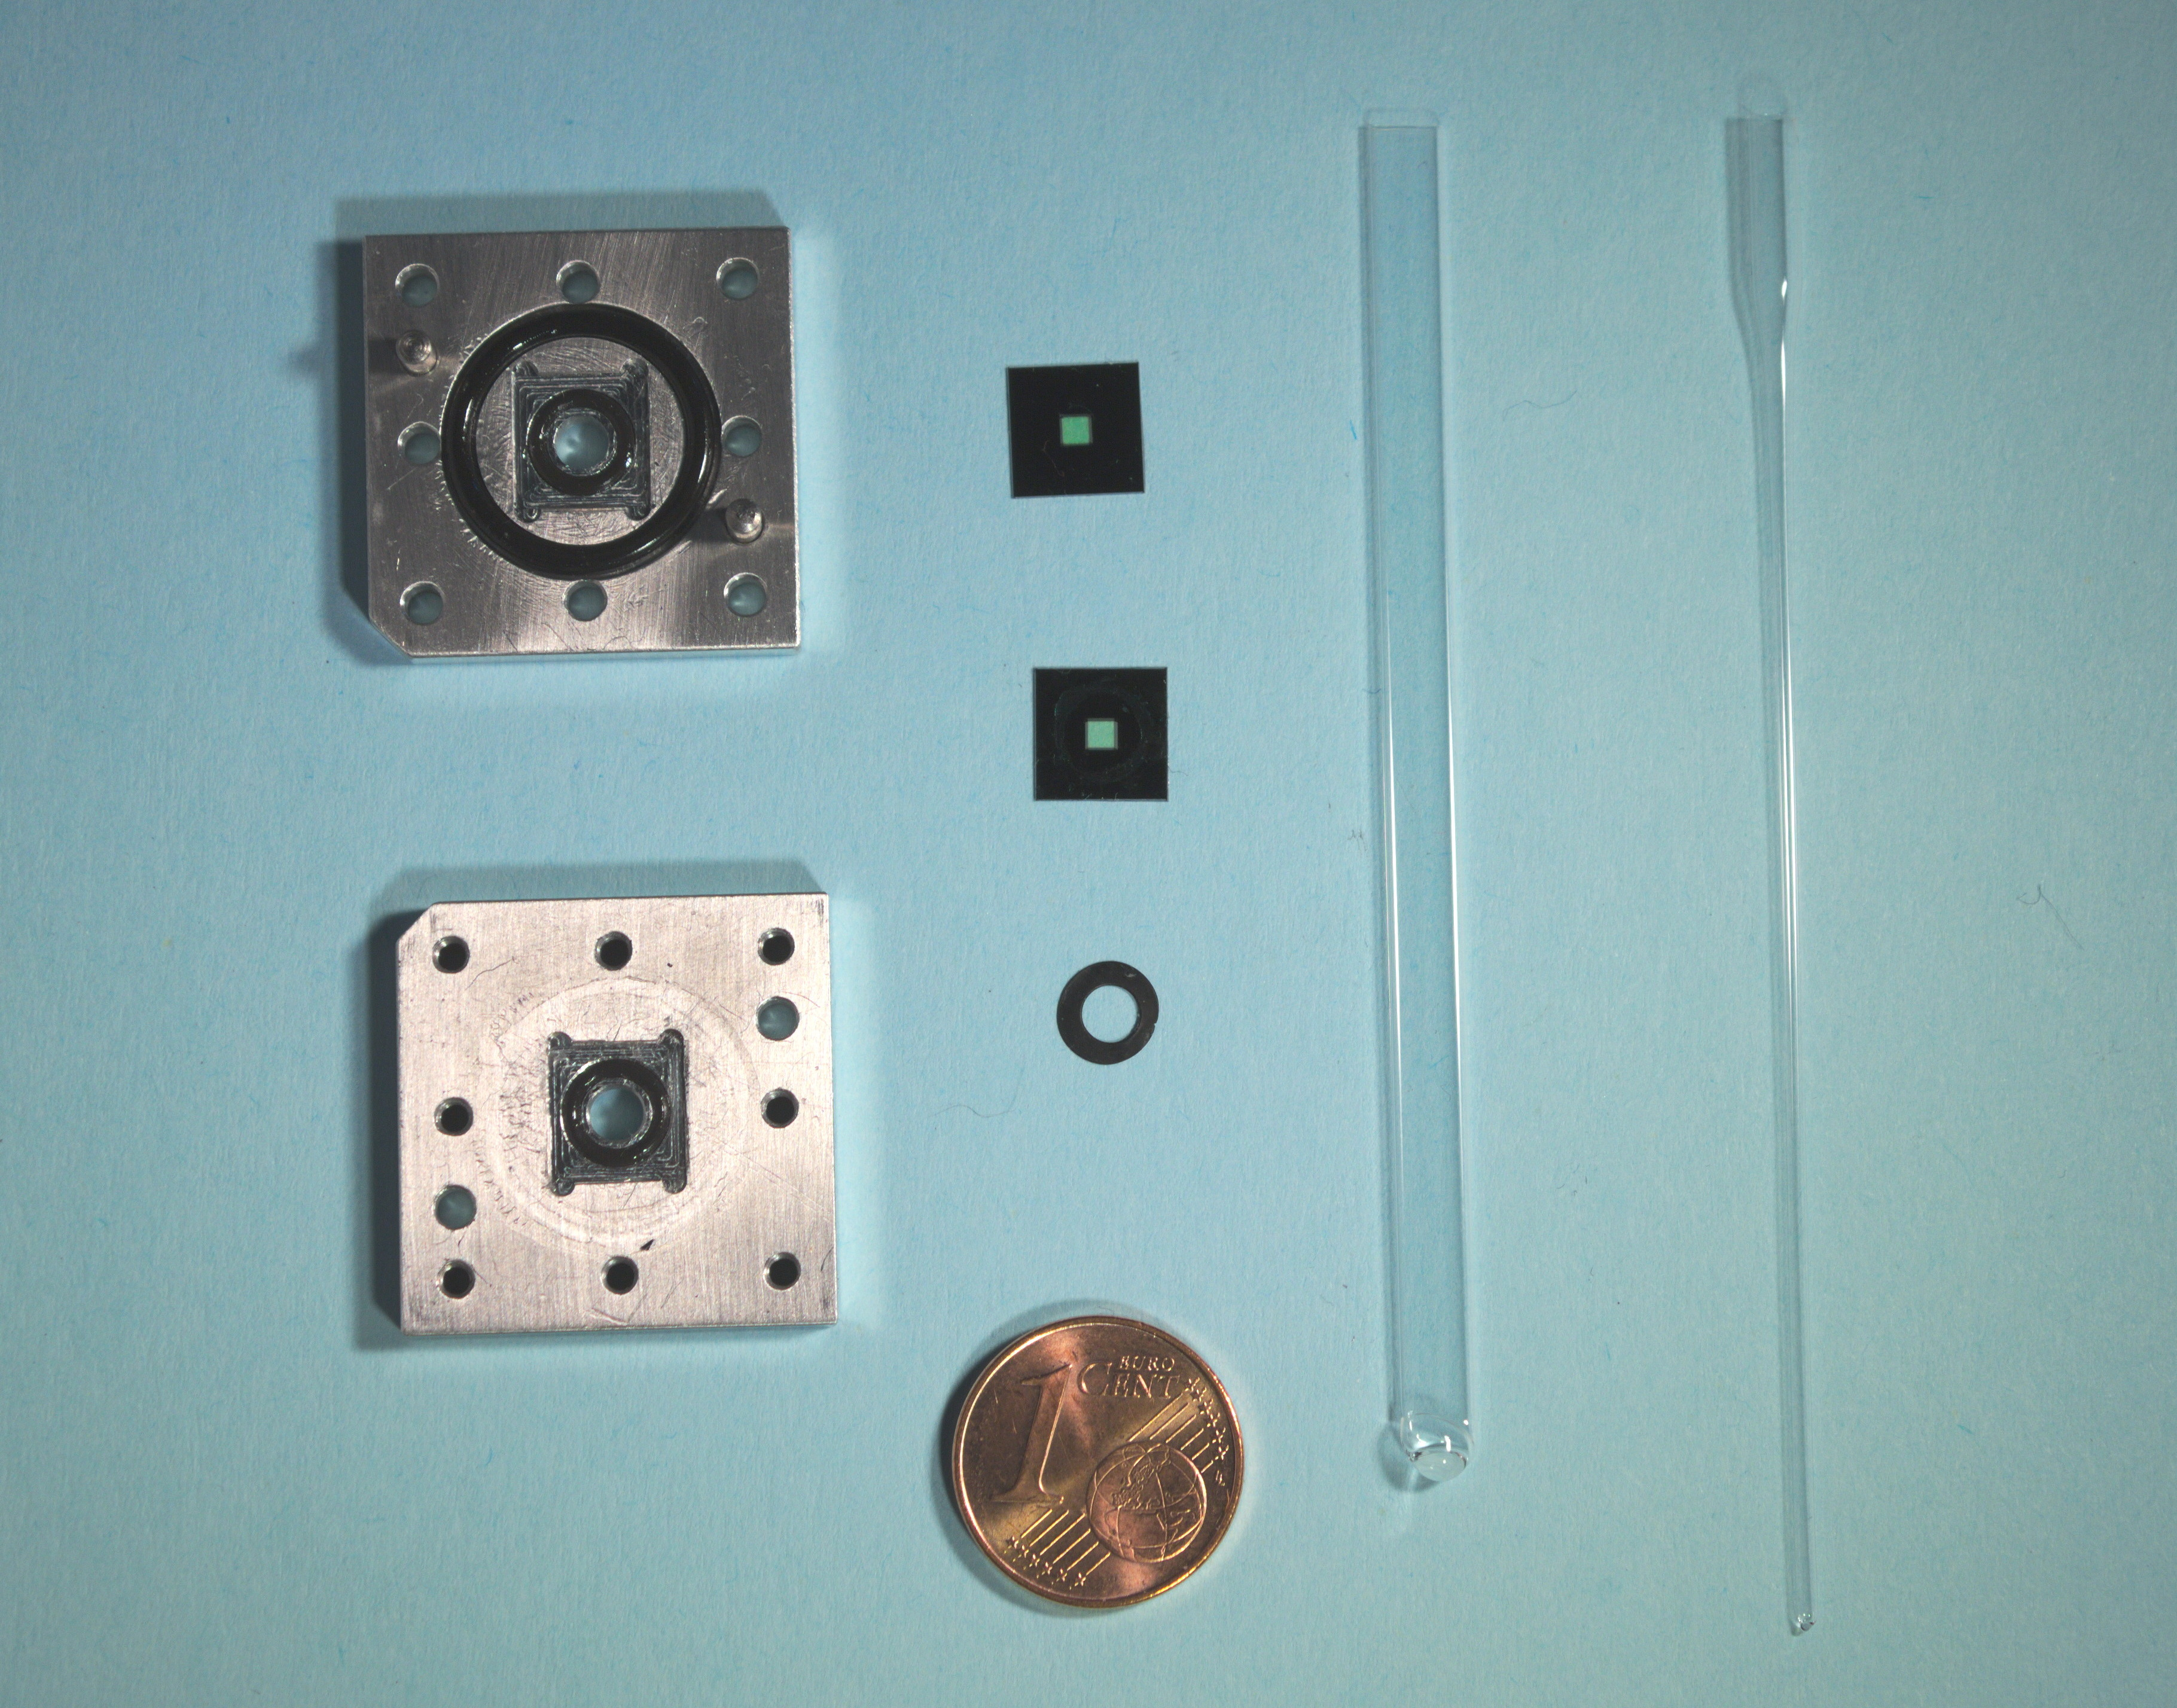
\includegraphics[width=0.9\linewidth]{Figures/SampleEnvironment.jpg}
		\caption[Sample environments for SAXS experiments in vacuum.]{Different sample environments: On the left side, the disassembled low-energy cell with the two silicon-nitride windows, the polymeric ring spacer and the two parts of the metallic holder. On the right side, the round and rectangular capillaries.}
	        \label{fig:SampleEnvironment}
\end{figure}

\section{Data reduction: The scattering curve}
\label{sec:data_reduction}

For isotropically scattering samples e.g. nanoparticles in suspension, the scattering patterns collected in the area detector consist of concentric rings whose center is the transmitted beam. The dimensionality of the data can be reduced by performing a radial integration of the measured pattern, converting the 2D images into 1D scattering curves. This reduction step is based on the $q$-binning: the grouping of pixels with similar scattering angle $q$ irrespective of their azimuthal angle on the detector \citep{pauw_everything_2013}. By averaging the scattered intensity of the pixels within the same $q$-bin ($I(q)$), the uncertainty of the data decreases in the scattering curve. The size of the bins depends on the requirements of the data evaluation while the bins are typically spaced uniformly, although logarithmic distributions are also extensively used. The difference in solid angle for each pixel due to the spherical projection of the scattering on a flat detector is also considered in this step.

The uncertainty associated to the intensity $I(q)$ is calculated as the standard deviation between each pixel intensity in the $q$-bin, which gives a better estimate than the uncertainty associated to the photon-counting Poisson statistics \citep{pauw_everything_2013}. The pixels discarded (or \emph{masked out}) for the weighted average of the $n$th $q$-bin ($q_n$) are those whose intensity is not comprised within the range 

\begin{equation}
\left[ \frac{\left|I_{\text{med}}\left( q_{n-1}\right)-I_{\text{med}}\left( q_{n}\right)\right|}{2} - 3 \sigma , \frac{\left|I_{\text{med}}\left( q_{n+1}\right)-I_{\text{med}}\left( q_{n}\right)\right|}{2} + 3 \sigma \right], 
\end{equation}

where $I_{\text{med}}\left( q_{n}\right)$ is the median intensity of the pixels prior to this \emph{masking procedure} and $\sigma$ is the standard deviation. With a confidence level of 99.7 $\%$, the pixels excluded of the reduction process are those pixels whose intensity lies clearly out of the radial average, such as \emph{hot pixels}, anisotropic scattering from the glass capillary or undesired reflexes without radial simmetry.

The position of the center of the scattering pattern is of vital importance for the radial integration step. A standard calibrant with very narrow diffraction rings such as AgBehe can be used to locate the center with high precision. Nevertheless, the masking process previously described can be used as well to determine the center position by minimizing the number of masked pixels and the standard deviation uncertainty of the $q$-bins. The accuracy of the center determination is sub-pixel using both approaches, but the masking procedure does not require a calibration standard material.

The scattering curve obtained by radial integration still requires of some data correction. For instance, $I_{\text{meas}}(q)$ (photon counts) must be normalized to the exposure time $\Delta t$, the solid angle $\Delta \Omega$, the measured transmittance of the sample $T$ and the incident photon flux $\Phi_0$, measured by the flux monitor described in section \ref{sec:fcm}. In order to present the scattering cross section per volume $\sfrac{d\Sigma}{d\Omega}$ in absolute units (cm$^{-1}$), the measured intensity must be normalized to the sample thickness $t$ and the quantum efficiencies of the X-ray detector and the silicon diodes $\eta_{QE}$: 

\begin{equation}
\frac{d\Sigma}{d\Omega} \left(q\right)=\frac{\frac{d\sigma}{d\Omega}\left(q\right)}{V} =\frac{I_{\text{meas}}\left(q\right)}{\Phi_0 \cdot T \cdot \Delta\Omega \cdot \Delta t \cdot \eta_{QE} \cdot t}
\end{equation}

By using the monitor diode on the beamstop as described in section \ref{sec:pilatus}, $T$ and $\Phi_0$ can be measured simultaneously during the experiment, without the necessity of the flux monitor diode.

Alternatively a standard material like lupolen \citep{kratky_absolute_1966,shaffer_calibration_1974} or glassy carbon \citep{perret_glassy_1972} can be employed to scale the measured scattering intensity to the known values of these materials.

The normalized scattering curve requires an accurate background correction. The scattering of the pure suspending medium and the sample environment can affect the evaluation of the data, specially for low-scatterers, and, therefore, the normalized scattering background must be subtracted to obtain a usable scattering curve.
